\documentclass[10pt,a4paper]{article}
\usepackage[utf8]{inputenc}
\usepackage[T1]{fontenc}
\usepackage{lmodern}
\usepackage[a4paper, margin=1.8cm, top=2.2cm, bottom=2.2cm, headheight=16pt, footskip=14pt]{geometry}
\usepackage{xcolor}
\usepackage{graphicx}
\usepackage{tikz}
\usepackage{amsmath,amssymb}
\usepackage{pifont}
\usepackage{fancyhdr}
\usepackage{titlesec}
\usepackage{microtype}
\usepackage{longtable}
\usepackage{booktabs}
\usepackage{array}
\usepackage{tcolorbox}
\usepackage{enumitem}
\usepackage{hyperref}

% Tight options list for questions
\newlist{qoptions}{enumerate}{1}
\setlist[qoptions]{label=\textbf{\Alph*.}, leftmargin=2em, itemsep=1.5pt, topsep=2.5pt, parsep=0pt}

% Color Definitions
\definecolor{hblue}{HTML}{1E3A8A}      % Navy Blue
\definecolor{hred}{HTML}{DC2626}       % Huawei Red accent
\definecolor{singlecol}{HTML}{0D9488}   % Teal for Single Choice
\definecolor{multicol}{HTML}{6D28D9}    % Purple for Multi Choice
\definecolor{tfcol}{HTML}{D97706}       % Amber for True/False
\definecolor{ansgreen}{HTML}{047857}    % Forest Green
\definecolor{ansbg}{HTML}{F0FDF4}       % Light Green Background
\definecolor{qbg}{HTML}{F8FAFC}         % Light Slate Background
\definecolor{qborder}{HTML}{CBD5E1}     % Border Slate
\definecolor{darkslate}{HTML}{1E293B}   % Slate 800

% Hyperref Setup
\hypersetup{
    colorlinks=true,
    linkcolor=hblue,
    citecolor=hblue,
    urlcolor=hblue,
    pdfauthor={Huawei ICT Academy / HCIA-Security Preparation},
    pdftitle={HCIA-Security Comprehensive Exam Question Bank},
    pdfsubject={HCIA-Security V3.0 Certification Exam Preparation},
    pdfkeywords={HCIA, Security, Huawei, Firewall, NAT, VRRP, IPS, PKI, IPsec, VPN}
}

% Header & Footer Configuration
\pagestyle{fancy}
\fancyhf{}
\fancyhead[L]{\small\color{darkslate!70}\textbf{HCIA-Security Exam Bank}}
\fancyhead[R]{\small\color{darkslate!70}\nouppercase{\leftmark}}
\fancyfoot[L]{\small\color{darkslate!50}Huawei Certified ICT Associate - Security}
\fancyfoot[R]{\small\color{darkslate!80}\textbf{Page \thepage}}
\renewcommand{\headrulewidth}{0.6pt}
\renewcommand{\footrulewidth}{0.4pt}

% Section Titles Styling
\titleformat{\part}[display]
  {\normalfont\huge\bfseries\centering\color{hblue}}
  {\Large\MakeUppercase{\partname} \thepart}
  {1ex}
  {\titlerule\vspace{1ex}\Huge}
  [\vspace{1ex}\titlerule]

\titleformat{\section}
  {\normalfont\Large\bfseries\color{hblue}}
  {\thesection}{1em}{}
  [\vspace{0.2ex}{\color{hblue}\titlerule[1.2pt]}]

\titleformat{\subsection}
  {\normalfont\large\bfseries\color{darkslate}}
  {\thesubsection}{0.8em}{}

% Custom Question Box
\newtcolorbox{qcard}[2]{
    colback=qbg,
    colframe=#2,
    arc=1.8mm,
    boxrule=0.7pt,
    leftrule=3.8pt,
    left=7pt,
    right=7pt,
    top=5pt,
    bottom=5pt,
    title={\textbf{Question #1}},
    coltitle=white,
    colbacktitle=#2,
    before=\par\vspace{0.6em}\noindent,
    after=\par\vspace{0.1em}
}

% Custom Explanation Box
\newtcolorbox{explainbox}[1]{
    colback=ansbg,
    colframe=ansgreen,
    arc=1.5mm,
    boxrule=0.5pt,
    leftrule=3.2pt,
    left=7pt,
    right=7pt,
    top=4pt,
    bottom=4pt,
    title={\small\textbf{Correct Answer: #1}},
    coltitle=white,
    colbacktitle=ansgreen,
    before=\par\vspace{0.1em}\noindent,
    after=\par\vspace{0.6em}
}


\begin{document}

% =========================================================================
% COVER / TITLE PAGE
% =========================================================================
\begin{titlepage}
    \centering
    \vspace*{0.4cm}
    
    % Official UM5R University Logo & Department Info
    
\includegraphics[height=2.4cm]{assets/um5r_logo.png}\par
    \vspace{0.35cm}
    {\fontsize{11}{14}\selectfont\scshape\bfseries\color{darkslate!90} Université Mohammed V de Rabat $\;\cdot\;$ Faculté des Sciences}\par
    \vspace{0.2cm}
    {\fontsize{11.5}{15}\selectfont\bfseries\color{hblue} Département d'Informatique $\;\cdot\;$ Master 2I2S}\par
    \vspace{0.15cm}
    {\fontsize{9.5}{12}\selectfont\itshape\color{darkslate!75} Ingénierie Informatique et Sécurité des Systèmes}\par
    \vspace{0.65cm}
    {\color{hblue!70}\rule{0.90\textwidth}{1.2pt}}\par
    \vspace{1.0cm}
    
    % Main Title Block
    {\fontsize{28}{34}\selectfont\bfseries\color{hblue} Huawei HCIA-Security V3.0\par}
    \vspace{0.35cm}
    {\fontsize{18}{22}\selectfont\bfseries\color{darkslate} Master 2I2S Exam Preparation Guide\par}
    \vspace{0.35cm}
    {\fontsize{12.5}{16}\selectfont\bfseries\color{singlecol!90!black} 1,050 Practice Questions with Detailed Explanations\par}
    \vspace{0.25cm}
    {\fontsize{10}{13}\selectfont\color{darkslate!65} Target Exam: \textbf{H12-711} $\;\cdot\;$ Huawei Certified ICT Associate -- Security\par}
    
    \vspace{1.1cm}
    
    % 3 Question Type Cards (Single Choice / Multi Choice / True False)
    \begin{center}
    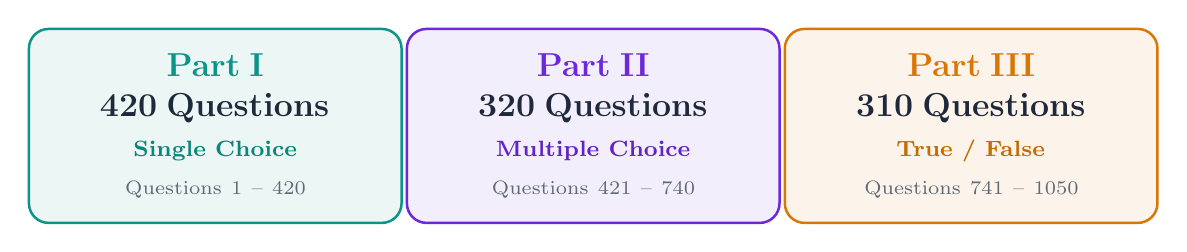
\begin{tikzpicture}
        % Single Choice
        \node[draw=singlecol, fill=singlecol!8, rounded corners=2.5mm, line width=0.9pt, inner sep=9pt, text width=4.1cm, align=center] at (-4.8,0) {
            {\bfseries\color{singlecol}\large Part I}\\[0.25em]
            {\bfseries\color{darkslate}\large 420 Questions}\\[0.25em]
            {\footnotesize\bfseries\color{singlecol!90!black} Single Choice}\\[0.15em]
            {\scriptsize\color{darkslate!70}Questions 1 -- 420}
        };
        % Multi Choice
        \node[draw=multicol, fill=multicol!8, rounded corners=2.5mm, line width=0.9pt, inner sep=9pt, text width=4.1cm, align=center] at (0,0) {
            {\bfseries\color{multicol}\large Part II}\\[0.25em]
            {\bfseries\color{darkslate}\large 320 Questions}\\[0.25em]
            {\footnotesize\bfseries\color{multicol!90!black} Multiple Choice}\\[0.15em]
            {\scriptsize\color{darkslate!70}Questions 421 -- 740}
        };
        % True / False
        \node[draw=tfcol, fill=tfcol!8, rounded corners=2.5mm, line width=0.9pt, inner sep=9pt, text width=4.1cm, align=center] at (4.8,0) {
            {\bfseries\color{tfcol}\large Part III}\\[0.25em]
            {\bfseries\color{darkslate}\large 310 Questions}\\[0.25em]
            {\footnotesize\bfseries\color{tfcol!90!black} True / False}\\[0.15em]
            {\scriptsize\color{darkslate!70}Questions 741 -- 1050}
        };
    \end{tikzpicture}
    \end{center}
    
    \vspace{0.9cm}
    
    % Clean Information Grid / Table of Exam Domains
    \begin{tcolorbox}[
        colback=qbg,
        colframe=hblue!25,
        arc=2.5mm,
        boxrule=0.8pt,
        width=0.90\textwidth,
        halign=left,
        top=11pt,
        bottom=11pt,
        left=16pt,
        right=16pt
    ]
        \centering
        {\bfseries\color{hblue}\normalsize Comprehensive Coverage of All 11 Exam Chapters}\\[0.6em]
        \renewcommand{\arraystretch}{1.25}
        \begin{tabular}{p{7.1cm}p{7.1cm}}
            {\small $\bullet$ \textbf{Ch 1-2:} Network Basics \& Attack Defense} & 
            {\small $\bullet$ \textbf{Ch 7:} Intrusion Prevention System (IPS)} \\
            {\small $\bullet$ \textbf{Ch 3:} Next-Gen Firewall Technologies} & 
            {\small $\bullet$ \textbf{Ch 8:} Cryptography Fundamentals} \\
            {\small $\bullet$ \textbf{Ch 4:} Network Address Translation (NAT)} & 
            {\small $\bullet$ \textbf{Ch 9:} PKI Certificate Architecture} \\
            {\small $\bullet$ \textbf{Ch 5:} Dual-System Hot Standby (VRRP/VGMP)} & 
            {\small $\bullet$ \textbf{Ch 10:} IPsec VPN Technologies} \\
            {\small $\bullet$ \textbf{Ch 6:} User Management \& AAA Security} & 
            {\small $\bullet$ \textbf{Ch 11:} SSL VPN Technologies} \\
        \end{tabular}\\[0.7em]
        {\footnotesize\color{ansgreen}\textbf{+ Complete Master Quick Answer Key Included (Pages 300--305)}}
    \end{tcolorbox}
    
    \vfill
    
    % Bottom Academic Meta Block
    {\color{hblue!40}\rule{0.90\textwidth}{0.8pt}}\par
    \vspace{0.45em}
    {\footnotesize\color{darkslate!75}
    \textbf{Université Mohammed V de Rabat} $\;\cdot\;$ Faculté des Sciences de Rabat\hfill \textbf{Academic Year 2025 -- 2026}\\[0.2em]
    \textbf{Master 2I2S} $\;\cdot\;$ Ingénierie Informatique et Sécurité des Systèmes\hfill \textbf{Student Revision Guide}
    }\par
    \vspace*{0.2cm}
\end{titlepage}

% =========================================================================
% TABLE OF CONTENTS
% =========================================================================
\tableofcontents
\clearpage

% =========================================================================
% EXAM BLUEPRINT & SYLLABUS OVERVIEW
% =========================================================================
\section*{HCIA-Security V3.0 Exam Blueprint \& Question Distribution}
\addcontentsline{toc}{section}{HCIA-Security V3.0 Exam Blueprint \& Question Distribution}

The Huawei Certified ICT Associate in Security (\textbf{HCIA-Security V3.0}, Exam Code: \textbf{H12-711}) validates that engineers possess foundational knowledge of enterprise network security architectures, Huawei firewall technologies, AAA user authentication, intrusion prevention, cryptographic principles, and VPN deployment. The examination consists of Single-Choice, Multiple-Choice, and True/False questions with a passing threshold of 600 out of 1000 points.

\vspace{0.8em}
\noindent This comprehensive question bank comprises \textbf{1,050 fully annotated questions} systematically organized into three distinct parts, spanning all 11 curriculum modules:

\begin{table}[h!]
\centering
\small
\begin{tabular}{clcccc}
\toprule
\textbf{Ch.} & \textbf{Chapter Curriculum Topic} & \textbf{Single (Pt 1)} & \textbf{Multi (Pt 2)} & \textbf{T/F (Pt 3)} & \textbf{Total Questions} \\
\midrule
1 & Network Security Concepts and Specifications & 36 & 26 & 26 & 88 \\
2 & Network Basics & 44 & 34 & 32 & 110 \\
3 & Common Network Security Threats and Threat Prevention & 36 & 28 & 26 & 90 \\
4 & Firewall Overview and Working Principles & 40 & 30 & 30 & 100 \\
5 & Firewall Security Policy and NAT Technology & 42 & 32 & 30 & 104 \\
6 & Firewall High Availability (VRRP & VGMP) & 38 & 30 & 28 & 96 \\
7 & User Management and AAA Technology & 38 & 30 & 28 & 96 \\
8 & Intrusion Prevention System (IPS) and Defense & 38 & 28 & 28 & 94 \\
9 & Cryptography Foundations and Encryption Technology & 34 & 26 & 25 & 85 \\
10 & PKI Certificate System and Applications & 34 & 26 & 25 & 85 \\
11 & Encryption Technology Applications (IPsec & SSL VPN) & 40 & 30 & 32 & 102 \\
\midrule
\textbf{--} & \textbf{Total Questions Across Curriculum} & \textbf{420} & \textbf{320} & \textbf{310} & \textbf{1050} \\
\bottomrule
\end{tabular}
\end{table}

\vspace{0.8em}
\noindent\textbf{Structure of Each Question Entry:}
\begin{itemize}[leftmargin=1.8em, itemsep=2pt]
    \item \textbf{Question Card:} Features the unique question number (QID), category accent color, specific syllabus topic tag, question stem, and standardized options (A, B, C, D).
    \item \textbf{Explanation Box:} Immediately follows each question card with the verified correct answer in the header, followed by an in-depth conceptual explanation elucidating \textit{why} the correct option is right, why distractors are incorrect, and the core Huawei HCIA-Security principle at work.
    \item \textbf{Quick Answer Key:} Appendix at the end of the volume featuring compact reference matrices for rapid self-assessment and mock exam scoring.
\end{itemize}
\clearpage


% =========================================================================
% PART 1: SINGLE-ANSWER QUESTIONS (Q1 - Q420)
% =========================================================================
\part{Single-Answer Questions (Q1 -- Q420)}
\section{Chapter 1: Network Security Concepts and Specifications}

\begin{qcard}{1}{singlecol}
\textcolor{darkslate!75}{\small\textbf{Topic:} CIA - Confidentiality \hfill \textbf{Type:} Single Choice}\vspace{0.4em}\par
Which security attribute ensures that sensitive information is not disclosed to unauthorized entities or eavesdropped during transmission?
\begin{qoptions}
\item Integrity
\item Confidentiality
\item Availability
\item Non-repudiation
\end{qoptions}
\end{qcard}
\nopagebreak
\begin{explainbox}{B}
\textbf{Concept \& Rationale:} Confidentiality ensures that information can be accessed and viewed only by authorized personnel. Cryptographic encryption is the primary mechanism to enforce confidentiality across untrusted networks.
\end{explainbox}

\begin{qcard}{2}{singlecol}
\textcolor{darkslate!75}{\small\textbf{Topic:} CIA - Integrity \hfill \textbf{Type:} Single Choice}\vspace{0.4em}\par
Which security property guarantees that transmitted data has not been altered, deleted, or forged in transit?
\begin{qoptions}
\item Availability
\item Integrity
\item Confidentiality
\item Authenticity
\end{qoptions}
\end{qcard}
\nopagebreak
\begin{explainbox}{B}
\textbf{Concept \& Rationale:} Integrity guarantees that data has not been tampered with or modified during transit or storage. Cryptographic hash functions (such as SHA-256) and message authentication codes are primary mechanisms to verify integrity.
\end{explainbox}

\begin{qcard}{3}{singlecol}
\textcolor{darkslate!75}{\small\textbf{Topic:} CIA - Availability \hfill \textbf{Type:} Single Choice}\vspace{0.4em}\par
An enterprise web service is taken down by a volumetric SYN flood attack, preventing legitimate clients from accessing their accounts. Which principle of the CIA triad has been violated?
\begin{qoptions}
\item Confidentiality
\item Integrity
\item Availability
\item Controllability
\end{qoptions}
\end{qcard}
\nopagebreak
\begin{explainbox}{C}
\textbf{Concept \& Rationale:} Availability ensures that authorized users have prompt and reliable access to information assets and network services. DoS/DDoS attacks specifically target availability by exhausting network bandwidth or server compute resources.
\end{explainbox}

\begin{qcard}{4}{singlecol}
\textcolor{darkslate!75}{\small\textbf{Topic:} Security Era - 1940s \hfill \textbf{Type:} Single Choice}\vspace{0.4em}\par
In the evolution of information security, what was the primary characteristic of the 'Communication Security' era during the 1940s?
\begin{qoptions}
\item Focus on cyberspace sovereignty and IoT devices
\item Protection was primarily confined to physical security and cipher-based transmission (mainly stream ciphers)
\item Emphasis on multi-dimensional active defense and SIEM orchestration
\item Standardization of enterprise security architectures such as ISO 27001
\end{qoptions}
\end{qcard}
\nopagebreak
\begin{explainbox}{B}
\textbf{Concept \& Rationale:} During the 1940s Communication Security era, communication technologies were underdeveloped. Information security focused on physical security and point-to-point cipher transmission (primarily stream ciphers) to protect confidential military and diplomatic telegrams.
\end{explainbox}

\begin{qcard}{5}{singlecol}
\textcolor{darkslate!75}{\small\textbf{Topic:} Security Era - 1990s \hfill \textbf{Type:} Single Choice}\vspace{0.4em}\par
During the 1990s Information Assurance period, which two new security principles were emphasized alongside the traditional CIA triad?
\begin{qoptions}
\item Simplicity and Scalability
\item Controllability and Non-repudiation
\item Virtualization and Micro-segmentation
\item Resilience and Fault-tolerance
\end{qoptions}
\end{qcard}
\nopagebreak
\begin{explainbox}{B}
\textbf{Concept \& Rationale:} In the 1990s Information Assurance era, as the Internet expanded rapidly, Controllability (ability to monitor and control information systems) and Non-repudiation (inability to deny transmitted actions/data) joined the CIA triad to form the five core security principles.
\end{explainbox}

\begin{qcard}{6}{singlecol}
\textcolor{darkslate!75}{\small\textbf{Topic:} Non-repudiation Mechanism \hfill \textbf{Type:} Single Choice}\vspace{0.4em}\par
Which cryptographic technology is primarily utilized to provide non-repudiation in electronic transactions?
\begin{qoptions}
\item Symmetric block ciphers like AES-256
\item Pre-shared keys (PSK)
\item Digital signatures using asymmetric private keys
\item Stream ciphers like RC4
\end{qoptions}
\end{qcard}
\nopagebreak
\begin{explainbox}{C}
\textbf{Concept \& Rationale:} Non-repudiation prevents a sender from denying having sent a message. It is achieved through digital signatures, where only the sender possesses the unique private key required to generate the signature.
\end{explainbox}

\begin{qcard}{7}{singlecol}
\textcolor{darkslate!75}{\small\textbf{Topic:} ISO Standards - ISO 27001 \hfill \textbf{Type:} Single Choice}\vspace{0.4em}\par
Which of the following standards specifies requirements for establishing, implementing, maintaining, and continually improving an Information Security Management System (ISMS) and is used for organizational certification?
\begin{qoptions}
\item ISO/IEC 27002
\item ISO/IEC 27001
\item ISO/IEC 27005
\item RFC 1918
\end{qoptions}
\end{qcard}
\nopagebreak
\begin{explainbox}{B}
\textbf{Concept \& Rationale:} ISO/IEC 27001 provides the formal normative specification for an enterprise Information Security Management System (ISMS) and serves as the certification benchmark. ISO 27002 provides guidance and codes of practice for implementing security controls.
\end{explainbox}

\begin{qcard}{8}{singlecol}
\textcolor{darkslate!75}{\small\textbf{Topic:} ISO Standards - ISO 27002 \hfill \textbf{Type:} Single Choice}\vspace{0.4em}\par
What is the primary role of ISO/IEC 27002 within the ISO 27000 series?
\begin{qoptions}
\item A formal audit standard against which an enterprise receives an accredited certificate
\item A code of practice containing reference control objectives and actionable security controls
\item A hardware encryption standard for high-speed fiber communications
\item A regulatory framework for national critical infrastructure penal sanctions
\end{qoptions}
\end{qcard}
\nopagebreak
\begin{explainbox}{B}
\textbf{Concept \& Rationale:} ISO/IEC 27002 provides a comprehensive code of practice and implementation guidelines for information security controls, helping organizations select and implement controls defined in Annex A of ISO 27001.
\end{explainbox}

\begin{qcard}{9}{singlecol}
\textcolor{darkslate!75}{\small\textbf{Topic:} Classified Protection - Levels Count \hfill \textbf{Type:} Single Choice}\vspace{0.4em}\par
Under Cybersecurity Classified Protection 2.0 (China's National Standard MLPS 2.0), how many security protection levels are defined?
\begin{qoptions}
\item Three levels
\item Four levels
\item Five levels
\item Seven levels
\end{qoptions}
\end{qcard}
\nopagebreak
\begin{explainbox}{C}
\textbf{Concept \& Rationale:} Classified Protection 2.0 defines five security levels: Level 1 (User Autonomy), Level 2 (System Audit), Level 3 (Supervised Protection), Level 4 (Mandatory Protection), and Level 5 (Special Control Protection).
\end{explainbox}

\begin{qcard}{10}{singlecol}
\textcolor{darkslate!75}{\small\textbf{Topic:} Classified Protection - Level 3 Impact \hfill \textbf{Type:} Single Choice}\vspace{0.4em}\par
In Classified Protection 2.0, Level 3 protection applies to information systems whose compromise would cause which severity of impact?
\begin{qoptions}
\item Slight harm to legitimate rights of citizens, but no harm to social order or public interest
\item Serious harm to social order and public interest, or harm to national security
\item Extremely serious harm to national security directly causing collapse of state governance
\item General harm to enterprise profitability without any public impact
\end{qoptions}
\end{qcard}
\nopagebreak
\begin{explainbox}{B}
\textbf{Concept \& Rationale:} Level 3 (Supervised Protection) applies to critical networks where security incidents cause serious harm to social order and public interests, or significant harm to national security. Most government and financial online systems require Level 3 compliance.
\end{explainbox}

\begin{qcard}{11}{singlecol}
\textcolor{darkslate!75}{\small\textbf{Topic:} TCSEC - Highest Division \hfill \textbf{Type:} Single Choice}\vspace{0.4em}\par
In the Trusted Computer System Evaluation Criteria (TCSEC, Orange Book), which division represents the highest level of security evaluation?
\begin{qoptions}
\item Division D
\item Division C
\item Division B
\item Division A
\end{qoptions}
\end{qcard}
\nopagebreak
\begin{explainbox}{D}
\textbf{Concept \& Rationale:} TCSEC categorizes systems into four divisions: D (Minimal protection), C (Discretionary protection: C1, C2), B (Mandatory protection: B1, B2, B3), and A (Verified protection: A1), where Division A is the highest verified security level.
\end{explainbox}

\begin{qcard}{12}{singlecol}
\textcolor{darkslate!75}{\small\textbf{Topic:} TCSEC - Class C2 \hfill \textbf{Type:} Single Choice}\vspace{0.4em}\par
Which TCSEC division and class introduced individual user identification and auditing requirements (Discretionary Access Control)?
\begin{qoptions}
\item Class D
\item Class C2
\item Class B2
\item Class A1
\end{qoptions}
\end{qcard}
\nopagebreak
\begin{explainbox}{B}
\textbf{Concept \& Rationale:} Class C2 (Controlled Access Protection) enforces individual login accountability, discretionary access control (DAC), and comprehensive audit trail logging, making it the historical baseline for commercial operating systems.
\end{explainbox}

\begin{qcard}{13}{singlecol}
\textcolor{darkslate!75}{\small\textbf{Topic:} APT Characteristics \hfill \textbf{Type:} Single Choice}\vspace{0.4em}\par
Which of the following is a prominent characteristic of an Advanced Persistent Threat (APT)?
\begin{qoptions}
\item Uncoordinated, short-duration high-volume automated ping sweeps
\item Highly organized, stealthy, customized, and persistent attack targeting high-value assets over an extended period
\item Purely accidental misconfigurations caused by novice network operators
\item Public Wi-Fi packet sniffing without target selection
\end{qoptions}
\end{qcard}
\nopagebreak
\begin{explainbox}{B}
\textbf{Concept \& Rationale:} An APT is characterized by advanced attack techniques, persistent reconnaissance, stealthy lateral movement, and evasion of conventional defenses, sustained over long durations to extract intellectual property or sabotage operations.
\end{explainbox}

\begin{qcard}{14}{singlecol}
\textcolor{darkslate!75}{\small\textbf{Topic:} Zero Trust Philosophy \hfill \textbf{Type:} Single Choice}\vspace{0.4em}\par
What is the foundational philosophy of the Zero Trust security model?
\begin{qoptions}
\item Trust internal network traffic by default; inspect only perimeter traffic
\item Never trust, always verify; inspect and authenticate every request regardless of network location
\item Rely solely on hardware border firewalls to defend the trusted core
\item Grant unrestricted administrative privileges once user identity is validated at login
\end{qoptions}
\end{qcard}
\nopagebreak
\begin{explainbox}{B}
\textbf{Concept \& Rationale:} Zero Trust operates under the tenet 'Never Trust, Always Verify'. It assumes breaches are inevitable, eliminating implicit trust based on network locality and requiring continuous verification of identity, device, and context.
\end{explainbox}

\begin{qcard}{15}{singlecol}
\textcolor{darkslate!75}{\small\textbf{Topic:} SDP Connectivity \hfill \textbf{Type:} Single Choice}\vspace{0.4em}\par
In a Software-Defined Perimeter (SDP) framework, how is network connectivity established?
\begin{qoptions}
\item Servers broadcast their IP and open ports publicly to allow direct client discovery
\item The infrastructure remains invisible ('dark') until an SDP controller validates user and device identity
\item Static security policies are permanently mapped to physical switch ports
\item All communications bypass encryption to accelerate line-rate throughput
\end{qoptions}
\end{qcard}
\nopagebreak
\begin{explainbox}{B}
\textbf{Concept \& Rationale:} SDP follows a 'Need-to-Know' paradigm where protected servers and services remain invisible behind Gateways. Connectivity is dynamically granted only after the centralized SDP Controller verifies client identity and device posture.
\end{explainbox}

\begin{qcard}{16}{singlecol}
\textcolor{darkslate!75}{\small\textbf{Topic:} Cybersecurity Legislation \hfill \textbf{Type:} Single Choice}\vspace{0.4em}\par
What is the primary objective of national cybersecurity laws and data security regulations?
\begin{qoptions}
\item To eliminate the need for enterprise firewalls and antivirus software
\item To safeguard cyberspace sovereignty, national security, public interest, and lawful citizen data rights
\item To mandate that all enterprise networks use unencrypted communication protocols
\item To replace internal enterprise security audits with foreign third-party certification
\end{qoptions}
\end{qcard}
\nopagebreak
\begin{explainbox}{B}
\textbf{Concept \& Rationale:} National cybersecurity regulations establish statutory obligations for network operators to protect critical infrastructure, maintain operational continuity, prevent cybercrimes, and protect citizens' personal privacy.
\end{explainbox}

\begin{qcard}{17}{singlecol}
\textcolor{darkslate!75}{\small\textbf{Topic:} Social Engineering - Phishing \hfill \textbf{Type:} Single Choice}\vspace{0.4em}\par
An attacker posing as an IT support engineer contacts an employee to obtain their domain credentials under the guise of an urgent security upgrade. What attack type is this?
\begin{qoptions}
\item Port scanning
\item Smurf attack
\item Social engineering / Phishing
\item Buffer overflow
\end{qoptions}
\end{qcard}
\nopagebreak
\begin{explainbox}{C}
\textbf{Concept \& Rationale:} Social engineering exploits human psychology rather than software vulnerabilities. Attackers use impersonation, pretexts, urgency, or deception to trick authorized personnel into disclosing credentials or sensitive data.
\end{explainbox}

\begin{qcard}{18}{singlecol}
\textcolor{darkslate!75}{\small\textbf{Topic:} Defense in Depth \hfill \textbf{Type:} Single Choice}\vspace{0.4em}\par
What is the fundamental benefit of implementing a 'Defense-in-Depth' architecture?
\begin{qoptions}
\item It guarantees 100\% immunity against zero-day malware without software updates
\item If a single defensive mechanism fails, multiple subsequent layers continue to protect critical assets
\item It eliminates the need for user authentication and authorization
\item It consolidates all security functions onto a single border router
\end{qoptions}
\end{qcard}
\nopagebreak
\begin{explainbox}{B}
\textbf{Concept \& Rationale:} Defense-in-Depth deploys multiple overlapping security controls across physical, perimeter, network, host, application, and data tiers, ensuring that compromise of any single layer does not compromise the entire enterprise.
\end{explainbox}

\begin{qcard}{19}{singlecol}
\textcolor{darkslate!75}{\small\textbf{Topic:} PDCA Cycle \hfill \textbf{Type:} Single Choice}\vspace{0.4em}\par
Which sequence correctly describes the continuous improvement lifecycle for enterprise security management?
\begin{qoptions}
\item Execute -\textgreater{} Terminate -\textgreater{} Delete -\textgreater{} Ignore
\item Plan -\textgreater{} Do -\textgreater{} Check -\textgreater{} Act (PDCA)
\item Attack -\textgreater{} Defend -\textgreater{} Forget -\textgreater{} Re-install
\item Inspect -\textgreater{} Block -\textgreater{} Allow -\textgreater{} Reset
\end{qoptions}
\end{qcard}
\nopagebreak
\begin{explainbox}{B}
\textbf{Concept \& Rationale:} The PDCA (Plan-Do-Check-Act) Deming cycle is the standard management framework adopted by ISO 27001 for establishing, maintaining, and continually optimizing organizational information security policies.
\end{explainbox}

\begin{qcard}{20}{singlecol}
\textcolor{darkslate!75}{\small\textbf{Topic:} Classified Protection - Tech Domains \hfill \textbf{Type:} Single Choice}\vspace{0.4em}\par
Which of the following is NOT one of the four general technical requirement domains in Classified Protection 2.0?
\begin{qoptions}
\item Physical and Environmental Security
\item Network and Communication Security
\item Equipment and Computing Security
\item Marketing and Public Relations Security
\end{qoptions}
\end{qcard}
\nopagebreak
\begin{explainbox}{D}
\textbf{Concept \& Rationale:} The four core technical requirement areas in Classified Protection 2.0 are: Physical and Environmental Security, Network and Communication Security, Equipment and Computing Security, and Application and Data Security.
\end{explainbox}

\begin{qcard}{21}{singlecol}
\textcolor{darkslate!75}{\small\textbf{Topic:} Classified Protection - Management Domains \hfill \textbf{Type:} Single Choice}\vspace{0.4em}\par
Which of the following belongs to the general security management requirements in Classified Protection 2.0?
\begin{qoptions}
\item Security Management System, Organization, Personnel, Construction, and Operation
\item Hardware BIOS Flashing and CPU Overclocking
\item External Advertising and Social Media Marketing
\item Quarterly Revenue Reporting and Tax Filing
\end{qoptions}
\end{qcard}
\nopagebreak
\begin{explainbox}{A}
\textbf{Concept \& Rationale:} The five management requirement domains under Classified Protection 2.0 comprise: Security Management System, Security Management Organization, Security Management Personnel, Security Construction Management, and Security Operation Management.
\end{explainbox}

\begin{qcard}{22}{singlecol}
\textcolor{darkslate!75}{\small\textbf{Topic:} Security Intelligence Center \hfill \textbf{Type:} Single Choice}\vspace{0.4em}\par
What is the primary function of a Security Intelligence Center (such as Huawei Cloud Security Intelligence)?
\begin{qoptions}
\item To remotely format local enterprise hard drives during high load
\item To aggregate global threat feeds, analyze zero-day exploits, and distribute real-time signature updates
\item To replace local enterprise network switches with software emulators
\item To permanently assign public IPv4 addresses to unauthorized mobile devices
\end{qoptions}
\end{qcard}
\nopagebreak
\begin{explainbox}{B}
\textbf{Concept \& Rationale:} Security Intelligence Centers analyze global telemetry, malware binaries, and emerging exploits using big data analytics and AI, producing up-to-date threat feeds, IPS/AV signatures, and malicious IP/domain blacklists.
\end{explainbox}

\begin{qcard}{23}{singlecol}
\textcolor{darkslate!75}{\small\textbf{Topic:} Cyberspace Characteristics \hfill \textbf{Type:} Single Choice}\vspace{0.4em}\par
Why is cyberspace considered an artificial, man-made operational domain compared to land, sea, air, and space?
\begin{qoptions}
\item It exists purely as a natural physical phenomenon without hardware
\item It is built upon physical microelectronics, logical network protocols, and software created by human engineering
\item It operates entirely without electrical power or telecommunication links
\item It is governed solely by international maritime law
\end{qoptions}
\end{qcard}
\nopagebreak
\begin{explainbox}{B}
\textbf{Concept \& Rationale:} Cyberspace is an engineered domain consisting of physical network infrastructure, logical software architectures, and cognitive human interaction, making it inherently dynamic and constantly evolving.
\end{explainbox}

\begin{qcard}{24}{singlecol}
\textcolor{darkslate!75}{\small\textbf{Topic:} Controllability Definition \hfill \textbf{Type:} Single Choice}\vspace{0.4em}\par
Under the five-pillar information security framework, what does 'Controllability' refer to?
\begin{qoptions}
\item Ensuring network bandwidth is throttled to 56 kbps at all times
\item Controlling information dissemination and maintaining administrative authority over information systems
\item Preventing any user from ever accessing external web servers
\item Eliminating all logging and auditing mechanisms on border firewalls
\end{qoptions}
\end{qcard}
\nopagebreak
\begin{explainbox}{B}
\textbf{Concept \& Rationale:} Controllability ensures that security administrators can monitor, audit, and regulate the lifecycle, flow, content, and system access of information assets, preventing unauthorized operations and policy violations.
\end{explainbox}

\begin{qcard}{25}{singlecol}
\textcolor{darkslate!75}{\small\textbf{Topic:} Ransomware Mechanism \hfill \textbf{Type:} Single Choice}\vspace{0.4em}\par
What is the primary economic extortion technique utilized by modern ransomware families?
\begin{qoptions}
\item Flooding target routers with ICMP echo requests until bandwidth saturation occurs
\item Silently modifying website HTML source code to display jokes without data loss
\item Encrypting critical organizational files with strong ciphers and demanding cryptocurrency for the private key
\item Stealing physical server chassis from locked enterprise datacenter racks
\end{qoptions}
\end{qcard}
\nopagebreak
\begin{explainbox}{C}
\textbf{Concept \& Rationale:} Ransomware uses high-grade symmetric and asymmetric cryptographic algorithms (e.g., AES-256 + RSA-2048) to encrypt user data in place, coercing victims into paying ransoms to obtain the decryption key.
\end{explainbox}

\begin{qcard}{26}{singlecol}
\textcolor{darkslate!75}{\small\textbf{Topic:} Vulnerability vs Exploit \hfill \textbf{Type:} Single Choice}\vspace{0.4em}\par
What is the technical distinction between a 'Vulnerability' and an 'Exploit'?
\begin{qoptions}
\item A vulnerability is malicious software code, whereas an exploit is a security standard
\item A vulnerability is a defect/weakness in software or hardware; an exploit is code or technique used to take advantage of it
\item A vulnerability only affects physical cables, while an exploit only affects web browsers
\item There is no distinction; both terms are exact synonyms in network engineering
\end{qoptions}
\end{qcard}
\nopagebreak
\begin{explainbox}{B}
\textbf{Concept \& Rationale:} A vulnerability is a flaw, bug, or design weakness present in software, protocols, or firmware. An exploit is a crafted payload, tool, or sequence of commands specifically constructed to take advantage of that vulnerability.
\end{explainbox}

\begin{qcard}{27}{singlecol}
\textcolor{darkslate!75}{\small\textbf{Topic:} Residual Risk \hfill \textbf{Type:} Single Choice}\vspace{0.4em}\par
What is 'Residual Risk' in enterprise risk management?
\begin{qoptions}
\item The initial risk measured before any security countermeasures are considered
\item The remaining risk that persists after appropriate security controls have been implemented
\item The risk that only affects obsolete hardware discarded in storage rooms
\item Risk that has been 100\% eliminated through cyber insurance
\end{qoptions}
\end{qcard}
\nopagebreak
\begin{explainbox}{B}
\textbf{Concept \& Rationale:} Residual risk is the remaining risk level after security controls, safeguards, and mitigation policies have been deployed. An organization must determine whether residual risk falls within its acceptable risk appetite.
\end{explainbox}

\begin{qcard}{28}{singlecol}
\textcolor{darkslate!75}{\small\textbf{Topic:} Security Awareness \hfill \textbf{Type:} Single Choice}\vspace{0.4em}\par
Why is regular security awareness training considered a critical component of enterprise security?
\begin{qoptions}
\item It completely replaces the need for technical controls like firewalls and IPS
\item Human errors and social engineering remain major attack vectors; user awareness mitigates phishing and policy violations
\item It guarantees that network equipment will never experience hardware power outages
\item It allows regular employees to rewrite firewall kernel code without supervision
\end{qoptions}
\end{qcard}
\nopagebreak
\begin{explainbox}{B}
\textbf{Concept \& Rationale:} Humans are frequently the weakest link in the security perimeter. Attackers leverage phishing and social engineering to bypass perimeter defenses; continuous training develops vigilance and adherence to security protocols.
\end{explainbox}

\begin{qcard}{29}{singlecol}
\textcolor{darkslate!75}{\small\textbf{Topic:} Asset Classification \hfill \textbf{Type:} Single Choice}\vspace{0.4em}\par
What is the first fundamental step in conducting an enterprise information security risk assessment?
\begin{qoptions}
\item Purchasing the most expensive firewall available on the market
\item Identifying and classifying organizational information assets based on business value and sensitivity
\item Disabling all incoming and outgoing Internet traffic across all branch offices
\item Assigning equal public administrative access to all internal and external users
\end{qoptions}
\end{qcard}
\nopagebreak
\begin{explainbox}{B}
\textbf{Concept \& Rationale:} Before risks can be assessed or mitigated, an organization must identify and catalog its critical assets (hardware, software, data, personnel) and categorize them according to confidentiality, integrity, and availability impact.
\end{explainbox}

\begin{qcard}{30}{singlecol}
\textcolor{darkslate!75}{\small\textbf{Topic:} Cyberspace Sovereignty \hfill \textbf{Type:} Single Choice}\vspace{0.4em}\par
How does the concept of national cyberspace sovereignty apply to digital communications?
\begin{qoptions}
\item Nation-states have independent jurisdiction over network infrastructure, data, and cyber activities within their sovereign territory
\item No government has the authority to regulate or protect domestic telecommunication systems
\item All data packets traversing global fiber optics are owned exclusively by international software vendors
\item Cyber activities are strictly exempt from domestic legal compliance
\end{qoptions}
\end{qcard}
\nopagebreak
\begin{explainbox}{A}
\textbf{Concept \& Rationale:} Cyberspace sovereignty reflects a state's independent jurisdiction and authority over its sovereign territory's cyber infrastructure, facilities, data governance, and legal accountability in cyberspace.
\end{explainbox}

\begin{qcard}{31}{singlecol}
\textcolor{darkslate!75}{\small\textbf{Topic:} Risk Transfer \hfill \textbf{Type:} Single Choice}\vspace{0.4em}\par
An enterprise decides to purchase cyber insurance to compensate for potential financial losses from data breaches. Which risk treatment strategy is being applied?
\begin{qoptions}
\item Risk Avoidance
\item Risk Mitigation
\item Risk Transfer
\item Risk Acceptance
\end{qoptions}
\end{qcard}
\nopagebreak
\begin{explainbox}{C}
\textbf{Concept \& Rationale:} Risk Transfer involves shifting financial liability or risk consequences to an external third party, commonly accomplished through cyber insurance policies or contractual outsourcing.
\end{explainbox}

\begin{qcard}{32}{singlecol}
\textcolor{darkslate!75}{\small\textbf{Topic:} Risk Acceptance \hfill \textbf{Type:} Single Choice}\vspace{0.4em}\par
When an organization formally decides to take no further action regarding an identified low-impact vulnerability because the cost of fixing it exceeds potential loss, this strategy is called:
\begin{qoptions}
\item Risk Avoidance
\item Risk Acceptance
\item Risk Transfer
\item Risk Exploitation
\end{qoptions}
\end{qcard}
\nopagebreak
\begin{explainbox}{B}
\textbf{Concept \& Rationale:} Risk Acceptance occurs when management formally acknowledges an identified risk and decides not to deploy countermeasures because the risk falls within acceptable tolerance or mitigation costs exceed the value of the asset.
\end{explainbox}

\begin{qcard}{33}{singlecol}
\textcolor{darkslate!75}{\small\textbf{Topic:} Defense in Depth - IAM \hfill \textbf{Type:} Single Choice}\vspace{0.4em}\par
In a multi-tier defense architecture, which security mechanism operates at the identity and access management layer?
\begin{qoptions}
\item Fiber optic intrusion detection sensor
\item Multi-Factor Authentication (MFA) and Least Privilege RBAC
\item BGP Route Reflector filtering
\item Shielded twisted pair copper grounding
\end{qoptions}
\end{qcard}
\nopagebreak
\begin{explainbox}{B}
\textbf{Concept \& Rationale:} Identity and Access Management (IAM) controls operate at the logical user tier, employing Multi-Factor Authentication (MFA), role-based access control (RBAC), and least privilege to enforce access boundaries.
\end{explainbox}

\begin{qcard}{34}{singlecol}
\textcolor{darkslate!75}{\small\textbf{Topic:} ISMS Purpose \hfill \textbf{Type:} Single Choice}\vspace{0.4em}\par
What is the core purpose of establishing an ISMS according to ISO 27001?
\begin{qoptions}
\item To build a systematic, ongoing management framework that identifies, manages, and minimizes security risks to corporate data
\item To replace all human employees with automated AI bots
\item To mandate the exclusive use of proprietary networking hardware
\item To produce marketing materials for social media advertising
\end{qoptions}
\end{qcard}
\nopagebreak
\begin{explainbox}{A}
\textbf{Concept \& Rationale:} An ISMS is a systematic framework comprising policies, processes, procedures, organizational structures, and software/hardware controls designed to manage and protect an organization's sensitive information assets.
\end{explainbox}

\begin{qcard}{35}{singlecol}
\textcolor{darkslate!75}{\small\textbf{Topic:} TCSEC B1 Mandatory Access Control \hfill \textbf{Type:} Single Choice}\vspace{0.4em}\par
What significant capability was introduced at the TCSEC Division B (specifically B1) level compared to Division C?
\begin{qoptions}
\item Elimination of all password authentication mechanisms
\item Mandatory Access Control (MAC) based on security labels and sensitivity levels
\item Unrestricted file sharing across all military networks without classification
\item Use of wireless Ethernet transmission without authentication
\end{qoptions}
\end{qcard}
\nopagebreak
\begin{explainbox}{B}
\textbf{Concept \& Rationale:} TCSEC Division B introduced Mandatory Access Control (MAC), where data objects and subjects carry formal security labels (e.g., Unclassified, Confidential, Secret, Top Secret), enforcing the Bell-LaPadula mathematical security model.
\end{explainbox}

\begin{qcard}{36}{singlecol}
\textcolor{darkslate!75}{\small\textbf{Topic:} Physical Security Priority \hfill \textbf{Type:} Single Choice}\vspace{0.4em}\par
Why does Classified Protection 2.0 list 'Physical and Environmental Security' as a mandatory technical domain?
\begin{qoptions}
\item Because physical access to server hardware bypasses logical controls, allowing direct storage extraction or hardware compromise
\item Because physical cables are immune to eavesdropping and environmental fire hazards
\item Because physical security replaces the necessity of IP routing protocols
\item Because server racks cannot operate unless painted in certified colors
\end{qoptions}
\end{qcard}
\nopagebreak
\begin{explainbox}{A}
\textbf{Concept \& Rationale:} Physical security is the bedrock of information assurance. If an adversary gains physical access to a server or network switch, logical controls (passwords, firewalls) can be circumvented via local console access, hardware implants, or direct drive extraction.
\end{explainbox}

\section{Chapter 2: Network Basics}

\begin{qcard}{37}{singlecol}
\textcolor{darkslate!75}{\small\textbf{Topic:} OSI Model Layers \hfill \textbf{Type:} Single Choice}\vspace{0.4em}\par
How many layers are defined in the Open Systems Interconnection (OSI) reference model?
\begin{qoptions}
\item 4 layers
\item 5 layers
\item 7 layers
\item 8 layers
\end{qoptions}
\end{qcard}
\nopagebreak
\begin{explainbox}{C}
\textbf{Concept \& Rationale:} The OSI reference model standardizes network communication into 7 distinct layers: Physical, Data Link, Network, Transport, Session, Presentation, and Application.
\end{explainbox}

\begin{qcard}{38}{singlecol}
\textcolor{darkslate!75}{\small\textbf{Topic:} OSI Layer 3 PDU \hfill \textbf{Type:} Single Choice}\vspace{0.4em}\par
What is the Protocol Data Unit (PDU) termed at Layer 3 (Network Layer) of the OSI model?
\begin{qoptions}
\item Bit
\item Frame
\item Packet
\item Segment
\end{qoptions}
\end{qcard}
\nopagebreak
\begin{explainbox}{C}
\textbf{Concept \& Rationale:} PDUs across OSI layers: Layer 1 = Bit; Layer 2 = Frame; Layer 3 = Packet; Layer 4 = Segment; Layers 5-7 = Data.
\end{explainbox}

\begin{qcard}{39}{singlecol}
\textcolor{darkslate!75}{\small\textbf{Topic:} OSI vs TCP/IP Mapping \hfill \textbf{Type:} Single Choice}\vspace{0.4em}\par
Which OSI layers are consolidated into the single Application layer in the 4-layer TCP/IP model?
\begin{qoptions}
\item Physical and Data Link layers
\item Data Link and Network layers
\item Session, Presentation, and Application layers
\item Transport and Session layers
\end{qoptions}
\end{qcard}
\nopagebreak
\begin{explainbox}{C}
\textbf{Concept \& Rationale:} The TCP/IP model merges the functions of OSI Layer 5 (Session), Layer 6 (Presentation), and Layer 7 (Application) into a single Application Layer.
\end{explainbox}

\begin{qcard}{40}{singlecol}
\textcolor{darkslate!75}{\small\textbf{Topic:} Ethernet Frame MAC Length \hfill \textbf{Type:} Single Choice}\vspace{0.4em}\par
In a standard Ethernet II frame, what is the length in bytes of the Destination MAC address field?
\begin{qoptions}
\item 4 bytes
\item 6 bytes
\item 8 bytes
\item 16 bytes
\end{qoptions}
\end{qcard}
\nopagebreak
\begin{explainbox}{B}
\textbf{Concept \& Rationale:} An Ethernet MAC address is 48 bits (6 bytes) long. An Ethernet II frame header contains a 6-byte Destination MAC followed by a 6-byte Source MAC and a 2-byte Type field.
\end{explainbox}

\begin{qcard}{41}{singlecol}
\textcolor{darkslate!75}{\small\textbf{Topic:} Ethernet EtherType IPv4 \hfill \textbf{Type:} Single Choice}\vspace{0.4em}\par
What is the hexadecimal EtherType value indicating that the payload of an Ethernet II frame is an IPv4 packet?
\begin{qoptions}
\item 0x0806
\item 0x0800
\item 0x86DD
\item 0x8100
\end{qoptions}
\end{qcard}
\nopagebreak
\begin{explainbox}{B}
\textbf{Concept \& Rationale:} Standard EtherType values: 0x0800 indicates IPv4; 0x0806 indicates ARP; 0x86DD indicates IPv6; 0x8100 indicates an IEEE 802.1Q tagged frame.
\end{explainbox}

\begin{qcard}{42}{singlecol}
\textcolor{darkslate!75}{\small\textbf{Topic:} Ethernet EtherType ARP \hfill \textbf{Type:} Single Choice}\vspace{0.4em}\par
Which EtherType value indicates an Address Resolution Protocol (ARP) frame?
\begin{qoptions}
\item 0x0800
\item 0x0806
\item 0x86DD
\item 0x8847
\end{qoptions}
\end{qcard}
\nopagebreak
\begin{explainbox}{B}
\textbf{Concept \& Rationale:} EtherType 0x0806 is assigned specifically to the Address Resolution Protocol (ARP).
\end{explainbox}

\begin{qcard}{43}{singlecol}
\textcolor{darkslate!75}{\small\textbf{Topic:} Ethernet MTU \hfill \textbf{Type:} Single Choice}\vspace{0.4em}\par
What is the standard default Maximum Transmission Unit (MTU) size for an Ethernet interface payload?
\begin{qoptions}
\item 576 bytes
\item 1480 bytes
\item 1500 bytes
\item 9000 bytes
\end{qoptions}
\end{qcard}
\nopagebreak
\begin{explainbox}{C}
\textbf{Concept \& Rationale:} The standard default MTU for Ethernet is 1500 bytes. This defines the maximum size of the Layer 3 packet (IP header + payload) that can be encapsulated into an Ethernet frame without fragmentation.
\end{explainbox}

\begin{qcard}{44}{singlecol}
\textcolor{darkslate!75}{\small\textbf{Topic:} IPv4 Header Minimum Size \hfill \textbf{Type:} Single Choice}\vspace{0.4em}\par
What is the minimum length of an IPv4 packet header when no optional fields are present?
\begin{qoptions}
\item 16 bytes
\item 20 bytes
\item 32 bytes
\item 40 bytes
\end{qoptions}
\end{qcard}
\nopagebreak
\begin{explainbox}{B}
\textbf{Concept \& Rationale:} The standard base IPv4 header with no options contains 5 rows of 32 bits (4 bytes) each, resulting in a minimum length of 20 bytes.
\end{explainbox}

\begin{qcard}{45}{singlecol}
\textcolor{darkslate!75}{\small\textbf{Topic:} IPv4 Header IHL Field \hfill \textbf{Type:} Single Choice}\vspace{0.4em}\par
In an IPv4 header, the Internet Header Length (IHL) field has a value of 5. How many total bytes does the IP header contain?
\begin{qoptions}
\item 5 bytes
\item 10 bytes
\item 20 bytes
\item 25 bytes
\end{qoptions}
\end{qcard}
\nopagebreak
\begin{explainbox}{C}
\textbf{Concept \& Rationale:} The IHL field specifies the IP header length in 32-bit (4-byte) words. Therefore, an IHL of 5 represents 5 * 4 = 20 bytes.
\end{explainbox}

\begin{qcard}{46}{singlecol}
\textcolor{darkslate!75}{\small\textbf{Topic:} IPv4 Header TTL Purpose \hfill \textbf{Type:} Single Choice}\vspace{0.4em}\par
What is the primary function of the Time to Live (TTL) field in an IPv4 header?
\begin{qoptions}
\item To record the exact timestamp when the packet was created
\item To prevent packets from circulating endlessly in routing loops
\item To calculate the round-trip latency between source and destination hosts
\item To negotiate the maximum TCP sliding window buffer size
\end{qoptions}
\end{qcard}
\nopagebreak
\begin{explainbox}{B}
\textbf{Concept \& Rationale:} The TTL field is decremented by 1 at each router hop. When TTL reaches 0, the packet is discarded and an ICMP Time Exceeded (Type 11) message is generated, preventing persistent routing loops.
\end{explainbox}

\begin{qcard}{47}{singlecol}
\textcolor{darkslate!75}{\small\textbf{Topic:} IPv4 Header Protocol TCP \hfill \textbf{Type:} Single Choice}\vspace{0.4em}\par
In the IPv4 header, what protocol value in the 'Protocol' field designates TCP?
\begin{qoptions}
\item 1
\item 6
\item 17
\item 47
\end{qoptions}
\end{qcard}
\nopagebreak
\begin{explainbox}{B}
\textbf{Concept \& Rationale:} Common IP Protocol numbers: 1 = ICMP; 6 = TCP; 17 = UDP; 47 = GRE; 50 = ESP; 51 = AH; 89 = OSPF.
\end{explainbox}

\begin{qcard}{48}{singlecol}
\textcolor{darkslate!75}{\small\textbf{Topic:} IPv4 Header Protocol UDP \hfill \textbf{Type:} Single Choice}\vspace{0.4em}\par
Which value in the IPv4 Protocol field identifies the payload as a User Datagram Protocol (UDP) segment?
\begin{qoptions}
\item 6
\item 17
\item 1
\item 88
\end{qoptions}
\end{qcard}
\nopagebreak
\begin{explainbox}{B}
\textbf{Concept \& Rationale:} Protocol number 17 designates UDP, while 6 designates TCP and 1 designates ICMP.
\end{explainbox}

\begin{qcard}{49}{singlecol}
\textcolor{darkslate!75}{\small\textbf{Topic:} IPv4 Header DF Flag \hfill \textbf{Type:} Single Choice}\vspace{0.4em}\par
Which flag in the IPv4 header instructs intermediate routers NOT to fragment the packet?
\begin{qoptions}
\item MF (More Fragments)
\item DF (Don't Fragment)
\item URG (Urgent)
\item SYN (Synchronize)
\end{qoptions}
\end{qcard}
\nopagebreak
\begin{explainbox}{B}
\textbf{Concept \& Rationale:} The DF (Don't Fragment) flag, when set to 1, instructs routers to drop the packet and send an ICMP Destination Unreachable (Fragmentation Needed, Type 3 Code 4) message if the packet exceeds the outgoing link's MTU.
\end{explainbox}

\begin{qcard}{50}{singlecol}
\textcolor{darkslate!75}{\small\textbf{Topic:} IPv4 RFC 1918 Private Ranges \hfill \textbf{Type:} Single Choice}\vspace{0.4em}\par
Which of the following IPv4 address blocks is designated as a private address space under RFC 1918?
\begin{qoptions}
\item 100.64.0.0/10
\item 172.16.0.0/12
\item 192.0.2.0/24
\item 169.254.0.0/16
\end{qoptions}
\end{qcard}
\nopagebreak
\begin{explainbox}{B}
\textbf{Concept \& Rationale:} RFC 1918 defines three private IPv4 address blocks: 10.0.0.0/8 (10.0.0.0 - 10.255.255.255), 172.16.0.0/12 (172.16.0.0 - 172.31.255.255), and 192.168.0.0/16 (192.168.0.0 - 192.168.255.255).
\end{explainbox}

\begin{qcard}{51}{singlecol}
\textcolor{darkslate!75}{\small\textbf{Topic:} IPv4 Class C Private Range \hfill \textbf{Type:} Single Choice}\vspace{0.4em}\par
What is the valid RFC 1918 private IPv4 range for Class C addresses?
\begin{qoptions}
\item 10.0.0.0 - 10.255.255.255
\item 172.16.0.0 - 172.31.255.255
\item 192.168.0.0 - 192.168.255.255
\item 192.168.1.0 - 192.168.1.255
\end{qoptions}
\end{qcard}
\nopagebreak
\begin{explainbox}{C}
\textbf{Concept \& Rationale:} The Class C private address space defined in RFC 1918 is 192.168.0.0/16, spanning from 192.168.0.0 to 192.168.255.255.
\end{explainbox}

\begin{qcard}{52}{singlecol}
\textcolor{darkslate!75}{\small\textbf{Topic:} IPv4 Loopback Address \hfill \textbf{Type:} Single Choice}\vspace{0.4em}\par
Which IPv4 address block is reserved by IANA for host internal loopback testing?
\begin{qoptions}
\item 0.0.0.0/8
\item 127.0.0.0/8
\item 169.254.0.0/16
\item 224.0.0.0/4
\end{qoptions}
\end{qcard}
\nopagebreak
\begin{explainbox}{B}
\textbf{Concept \& Rationale:} The entire 127.0.0.0/8 block is reserved for loopback operations. Traffic sent to 127.0.0.1 is looped back internally within the host IP stack without reaching physical media.
\end{explainbox}

\begin{qcard}{53}{singlecol}
\textcolor{darkslate!75}{\small\textbf{Topic:} Subnetting Usable Hosts /27 \hfill \textbf{Type:} Single Choice}\vspace{0.4em}\par
How many usable host IP addresses are available in an IPv4 subnet with a /27 prefix (mask 255.255.255.224)?
\begin{qoptions}
\item 14
\item 30
\item 32
\item 62
\end{qoptions}
\end{qcard}
\nopagebreak
\begin{explainbox}{B}
\textbf{Concept \& Rationale:} A /27 subnet has 32 - 27 = 5 host bits. Total addresses = 2\textasciicircum{}5 = 32. Subtracting the network address and directed broadcast address yields 32 - 2 = 30 usable host IP addresses.
\end{explainbox}

\begin{qcard}{54}{singlecol}
\textcolor{darkslate!75}{\small\textbf{Topic:} Subnetting Broadcast Address \hfill \textbf{Type:} Single Choice}\vspace{0.4em}\par
What is the directed broadcast address for the subnet 192.168.1.64/26?
\begin{qoptions}
\item 192.168.1.64
\item 192.168.1.127
\item 192.168.1.128
\item 192.168.1.255
\end{qoptions}
\end{qcard}
\nopagebreak
\begin{explainbox}{B}
\textbf{Concept \& Rationale:} A /26 subnet has block size 256 - 192 = 64. Subnet range: 192.168.1.64 to 192.168.1.127. The first address (.64) is network ID, and the last (.127) is the directed broadcast address.
\end{explainbox}

\begin{qcard}{55}{singlecol}
\textcolor{darkslate!75}{\small\textbf{Topic:} ARP Request Mode \hfill \textbf{Type:} Single Choice}\vspace{0.4em}\par
How is an initial ARP Request frame transmitted across a local broadcast domain to resolve a target IP address?
\begin{qoptions}
\item Unicast to the default gateway
\item Broadcast (Destination MAC FF:FF:FF:FF:FF:FF)
\item Multicast to 224.0.0.1
\item Anycast across all router ports
\end{qoptions}
\end{qcard}
\nopagebreak
\begin{explainbox}{B}
\textbf{Concept \& Rationale:} Because the sending host does not know the destination MAC address, it broadcasts the ARP Request with Destination MAC FF:FF:FF:FF:FF:FF so all hosts on the local link process it.
\end{explainbox}

\begin{qcard}{56}{singlecol}
\textcolor{darkslate!75}{\small\textbf{Topic:} ARP Reply Mode \hfill \textbf{Type:} Single Choice}\vspace{0.4em}\par
How does the target host respond to an ARP Request?
\begin{qoptions}
\item It broadcasts the ARP Reply to all hosts
\item It transmits a unicast ARP Reply directly to the requester's MAC address
\item It transmits an ICMP Echo Reply
\item It registers its MAC address with the DNS server
\end{qoptions}
\end{qcard}
\nopagebreak
\begin{explainbox}{B}
\textbf{Concept \& Rationale:} The target host learned the requester's MAC and IP addresses from the ARP Request header. Thus, it responds with a unicast ARP Reply directly addressed to the requester.
\end{explainbox}

\begin{qcard}{57}{singlecol}
\textcolor{darkslate!75}{\small\textbf{Topic:} Gratuitous ARP Function \hfill \textbf{Type:} Single Choice}\vspace{0.4em}\par
What is a primary purpose of transmitting a Gratuitous ARP packet?
\begin{qoptions}
\item To query the DNS root server for top-level domains
\item To detect duplicate IP address conflicts and update neighbors' ARP mapping caches
\item To authenticate user credentials against a RADIUS server
\item To establish an encrypted IPsec tunnel across the WAN
\end{qoptions}
\end{qcard}
\nopagebreak
\begin{explainbox}{B}
\textbf{Concept \& Rationale:} A host broadcasts a Gratuitous ARP (where source IP and target IP are its own address) upon interface activation to check if another device is already using that IP address (conflict detection) and to update MAC-to-IP tables on switches and neighbors.
\end{explainbox}

\begin{qcard}{58}{singlecol}
\textcolor{darkslate!75}{\small\textbf{Topic:} Proxy ARP Function \hfill \textbf{Type:} Single Choice}\vspace{0.4em}\par
What is the function of Proxy ARP on a router or firewall interface?
\begin{qoptions}
\item To encrypt all ARP queries using AES-128
\item To respond with its own MAC address to an ARP request on behalf of a target host located on another subnet
\item To permanently block all ARP traffic entering the interface
\item To translate IPv4 addresses to IPv6 addresses
\end{qoptions}
\end{qcard}
\nopagebreak
\begin{explainbox}{B}
\textbf{Concept \& Rationale:} Proxy ARP allows a router or firewall to reply with its own MAC address to an ARP Request sent by a local host seeking a destination host on a different subnet/network, enabling communication without configuring default gateways on legacy hosts.
\end{explainbox}

\begin{qcard}{59}{singlecol}
\textcolor{darkslate!75}{\small\textbf{Topic:} ICMP Protocol Layer \hfill \textbf{Type:} Single Choice}\vspace{0.4em}\par
At which OSI layer does the Internet Control Message Protocol (ICMP) logically operate, and how is it encapsulated?
\begin{qoptions}
\item Layer 2, encapsulated directly inside Ethernet frames
\item Layer 3, encapsulated directly inside IPv4 packets (Protocol 1)
\item Layer 4, encapsulated inside TCP segments
\item Layer 7, encapsulated inside HTTP requests
\end{qoptions}
\end{qcard}
\nopagebreak
\begin{explainbox}{B}
\textbf{Concept \& Rationale:} ICMP is an integral part of the Network Layer (Layer 3). Its messages are encapsulated directly within IP datagrams with the IP header Protocol field set to 1.
\end{explainbox}

\begin{qcard}{60}{singlecol}
\textcolor{darkslate!75}{\small\textbf{Topic:} ICMP Ping Echo Request \hfill \textbf{Type:} Single Choice}\vspace{0.4em}\par
What are the ICMP Type and Code values for an ICMP Echo Request (Ping request)?
\begin{qoptions}
\item Type 0, Code 0
\item Type 8, Code 0
\item Type 3, Code 1
\item Type 11, Code 0
\end{qoptions}
\end{qcard}
\nopagebreak
\begin{explainbox}{B}
\textbf{Concept \& Rationale:} An ICMP Echo Request utilizes Type 8, Code 0. The responding device replies with an ICMP Echo Reply using Type 0, Code 0.
\end{explainbox}

\begin{qcard}{61}{singlecol}
\textcolor{darkslate!75}{\small\textbf{Topic:} ICMP Destination Unreachable \hfill \textbf{Type:} Single Choice}\vspace{0.4em}\par
Which ICMP Type indicates that a destination network, host, port, or protocol is unreachable?
\begin{qoptions}
\item Type 0
\item Type 3
\item Type 8
\item Type 11
\end{qoptions}
\end{qcard}
\nopagebreak
\begin{explainbox}{B}
\textbf{Concept \& Rationale:} ICMP Type 3 represents 'Destination Unreachable'. Specific codes include Code 0 (Network Unreachable), Code 1 (Host Unreachable), Code 3 (Port Unreachable), and Code 4 (Fragmentation Needed and DF set).
\end{explainbox}

\begin{qcard}{62}{singlecol}
\textcolor{darkslate!75}{\small\textbf{Topic:} ICMP Traceroute Type \hfill \textbf{Type:} Single Choice}\vspace{0.4em}\par
Which ICMP message is generated by intermediate routers when their TTL counter reaches zero, enabling the 'tracert' / 'traceroute' command?
\begin{qoptions}
\item Type 0 Echo Reply
\item Type 3 Destination Unreachable
\item Type 11 Time Exceeded
\item Type 5 Redirect
\end{qoptions}
\end{qcard}
\nopagebreak
\begin{explainbox}{C}
\textbf{Concept \& Rationale:} Traceroute transmits packets with incrementing TTL values starting at 1. When a router decrements TTL to 0, it drops the packet and sends an ICMP Type 11 (Time Exceeded) message back to the source, revealing that hop's IP address.
\end{explainbox}

\begin{qcard}{63}{singlecol}
\textcolor{darkslate!75}{\small\textbf{Topic:} TCP Characteristics \hfill \textbf{Type:} Single Choice}\vspace{0.4em}\par
Which of the following is a key operational characteristic of Transmission Control Protocol (TCP)?
\begin{qoptions}
\item Connectionless, best-effort delivery without acknowledgments
\item Connection-oriented, reliable byte-stream service with error recovery and flow control
\item Stateless broadcast transmission across local networks
\item Fixed 8-byte header size with no options
\end{qoptions}
\end{qcard}
\nopagebreak
\begin{explainbox}{B}
\textbf{Concept \& Rationale:} TCP (RFC 793) is a connection-oriented, reliable transport protocol that provides sequencing, acknowledgments, sliding-window flow control, congestion avoidance, and retransmission of lost segments.
\end{explainbox}

\begin{qcard}{64}{singlecol}
\textcolor{darkslate!75}{\small\textbf{Topic:} TCP Handshake Flags \hfill \textbf{Type:} Single Choice}\vspace{0.4em}\par
What is the correct sequence of TCP flag exchanges during connection establishment?
\begin{qoptions}
\item ACK -\textgreater{} SYN -\textgreater{} FIN
\item SYN -\textgreater{} SYN-ACK -\textgreater{} ACK
\item SYN -\textgreater{} ACK-FIN -\textgreater{} RST
\item RST -\textgreater{} SYN -\textgreater{} ACK
\end{qoptions}
\end{qcard}
\nopagebreak
\begin{explainbox}{B}
\textbf{Concept \& Rationale:} The TCP 3-way handshake begins with the client sending a SYN segment, the server responding with SYN-ACK, and the client confirming with an ACK segment, transitioning the connection to the ESTABLISHED state.
\end{explainbox}

\begin{qcard}{65}{singlecol}
\textcolor{darkslate!75}{\small\textbf{Topic:} TCP Termination Segments \hfill \textbf{Type:} Single Choice}\vspace{0.4em}\par
How many segments are typically exchanged to gracefully close a bidirectional TCP connection?
\begin{qoptions}
\item 2 segments
\item 3 segments
\item 4 segments (FIN -\textgreater{} ACK -\textgreater{} FIN -\textgreater{} ACK)
\item 6 segments
\end{qoptions}
\end{qcard}
\nopagebreak
\begin{explainbox}{C}
\textbf{Concept \& Rationale:} Because TCP is full-duplex, each direction of data transfer closes independently. Host A sends FIN, Host B sends ACK (closing A-\textgreater{}B); then Host B sends FIN, and Host A sends ACK (closing B-\textgreater{}A), totaling 4 segments.
\end{explainbox}

\begin{qcard}{66}{singlecol}
\textcolor{darkslate!75}{\small\textbf{Topic:} TCP TIME\_WAIT Rationale \hfill \textbf{Type:} Single Choice}\vspace{0.4em}\par
What is the primary reason the TCP active close endpoint remains in the TIME\_WAIT state for 2 MSL (Maximum Segment Lifetime)?
\begin{qoptions}
\item To immediately renegotiate encryption keys for the next connection
\item To ensure the final ACK is received by the peer and allow old duplicate segments to expire in the network
\item To allow the server to recharge its hardware interface buffers
\item To force the client to restart its operating system
\end{qoptions}
\end{qcard}
\nopagebreak
\begin{explainbox}{B}
\textbf{Concept \& Rationale:} The 2 MSL TIME\_WAIT state ensures that if the final ACK is lost, the retransmitted FIN can be acknowledged. It also guarantees that all delayed segments from the closed connection expire and cannot corrupt future connections using the same socket pair.
\end{explainbox}

\begin{qcard}{67}{singlecol}
\textcolor{darkslate!75}{\small\textbf{Topic:} TCP RST Flag \hfill \textbf{Type:} Single Choice}\vspace{0.4em}\par
What is the function of the RST (Reset) flag in a TCP header?
\begin{qoptions}
\item To request dynamic routing table updates from adjacent firewalls
\item To abort an abnormal connection immediately and reject invalid connection attempts
\item To initiate the graceful 3-way handshake
\item To indicate that urgent out-of-band data is present
\end{qoptions}
\end{qcard}
\nopagebreak
\begin{explainbox}{B}
\textbf{Concept \& Rationale:} The RST flag resets an invalid connection, aborts an active session due to errors, or rejects an incoming SYN directed to an inactive/closed port.
\end{explainbox}

\begin{qcard}{68}{singlecol}
\textcolor{darkslate!75}{\small\textbf{Topic:} UDP Header Length \hfill \textbf{Type:} Single Choice}\vspace{0.4em}\par
What is the fixed header size of a standard User Datagram Protocol (UDP) segment?
\begin{qoptions}
\item 8 bytes
\item 16 bytes
\item 20 bytes
\item 32 bytes
\end{qoptions}
\end{qcard}
\nopagebreak
\begin{explainbox}{A}
\textbf{Concept \& Rationale:} A UDP header contains exactly four 16-bit fields: Source Port (2 bytes), Destination Port (2 bytes), Length (2 bytes), and Checksum (2 bytes), totaling 8 bytes.
\end{explainbox}

\begin{qcard}{69}{singlecol}
\textcolor{darkslate!75}{\small\textbf{Topic:} UDP Real-Time Media \hfill \textbf{Type:} Single Choice}\vspace{0.4em}\par
Why is UDP preferred over TCP for real-time voice and video streaming (e.g., VoIP, video conferencing)?
\begin{qoptions}
\item UDP provides stronger encryption algorithms than TCP
\item UDP has low latency and no retransmission delays, prioritizing timely delivery over perfect reliability
\item UDP guarantees 100\% loss-free packet delivery across congested links
\item UDP automatically modifies router forwarding tables to prevent jitter
\end{qoptions}
\end{qcard}
\nopagebreak
\begin{explainbox}{B}
\textbf{Concept \& Rationale:} Real-time media applications prioritize low latency and predictable jitter. Retransmitting dropped audio/video frames via TCP causes noticeable lag and freezes; dropping occasional packets is preferable.
\end{explainbox}

\begin{qcard}{70}{singlecol}
\textcolor{darkslate!75}{\small\textbf{Topic:} DNS Query Transport \hfill \textbf{Type:} Single Choice}\vspace{0.4em}\par
Which transport protocol and port number are predominantly used by standard DNS client queries?
\begin{qoptions}
\item TCP port 25
\item UDP port 53
\item TCP port 80
\item UDP port 67
\end{qoptions}
\end{qcard}
\nopagebreak
\begin{explainbox}{B}
\textbf{Concept \& Rationale:} Standard DNS queries and responses utilize UDP port 53 for speed. DNS uses TCP port 53 for responses exceeding 512 bytes (or EDNS0 limits) and for zone transfers between DNS servers.
\end{explainbox}

\begin{qcard}{71}{singlecol}
\textcolor{darkslate!75}{\small\textbf{Topic:} DNS Record Type A \hfill \textbf{Type:} Single Choice}\vspace{0.4em}\par
Which DNS resource record type maps a fully qualified domain name (FQDN) to an IPv4 address?
\begin{qoptions}
\item AAAA record
\item A record
\item CNAME record
\item PTR record
\end{qoptions}
\end{qcard}
\nopagebreak
\begin{explainbox}{B}
\textbf{Concept \& Rationale:} An 'A' record maps a hostname to an IPv4 address. 'AAAA' maps to IPv6; 'CNAME' maps an alias to a canonical name; 'PTR' provides reverse resolution from IP to domain name.
\end{explainbox}

\begin{qcard}{72}{singlecol}
\textcolor{darkslate!75}{\small\textbf{Topic:} HTTP HTTPS Default Ports \hfill \textbf{Type:} Single Choice}\vspace{0.4em}\par
What are the default standard TCP ports for unencrypted HTTP and encrypted HTTPS, respectively?
\begin{qoptions}
\item HTTP: 21, HTTPS: 22
\item HTTP: 80, HTTPS: 443
\item HTTP: 8080, HTTPS: 8443
\item HTTP: 25, HTTPS: 587
\end{qoptions}
\end{qcard}
\nopagebreak
\begin{explainbox}{B}
\textbf{Concept \& Rationale:} Standard HTTP communicates over cleartext TCP port 80, whereas HTTPS encrypts HTTP traffic inside TLS/SSL over TCP port 443.
\end{explainbox}

\begin{qcard}{73}{singlecol}
\textcolor{darkslate!75}{\small\textbf{Topic:} FTP Control and Data Ports \hfill \textbf{Type:} Single Choice}\vspace{0.4em}\par
In traditional Active Mode File Transfer Protocol (FTP), which port is used for control commands and which for data transfer?
\begin{qoptions}
\item Port 21 for Control; Port 20 for Data
\item Port 22 for Control; Port 21 for Data
\item Port 80 for Control; Port 443 for Data
\item Port 69 for Control; Port 68 for Data
\end{qoptions}
\end{qcard}
\nopagebreak
\begin{explainbox}{A}
\textbf{Concept \& Rationale:} FTP separates control commands from data transfer. Port 21 is the command/control port, while the FTP server initiates data connections from port 20 in Active FTP mode.
\end{explainbox}

\begin{qcard}{74}{singlecol}
\textcolor{darkslate!75}{\small\textbf{Topic:} FTP Active Mode NAT Problem \hfill \textbf{Type:} Single Choice}\vspace{0.4em}\par
Why does Active FTP fail when the FTP client is located behind a standard NAT router/firewall?
\begin{qoptions}
\item The client refuses to communicate with servers running Linux
\item The FTP server initiates an inbound connection from port 20 to the client's high port, which the client firewall blocks
\item Active FTP requires uncompressed video streaming bandwidth
\item NAT devices are physically prohibited from handling TCP port 21
\end{qoptions}
\end{qcard}
\nopagebreak
\begin{explainbox}{B}
\textbf{Concept \& Rationale:} In Active FTP, the client sends a PORT command specifying its internal IP and high port, then listens. The server initiates an incoming connection from port 20 to that port. A stateful firewall or NAT device at the client border blocks this unsolicited incoming connection unless an FTP ALG/ASPF is active.
\end{explainbox}

\begin{qcard}{75}{singlecol}
\textcolor{darkslate!75}{\small\textbf{Topic:} FTP Passive Mode Solution \hfill \textbf{Type:} Single Choice}\vspace{0.4em}\par
How does Passive FTP (PASV) resolve client-side firewall and NAT traversal issues?
\begin{qoptions}
\item The server initiates the data connection directly to port 80
\item The server opens a random high port and the client initiates the outbound data connection to that port
\item Passive FTP disables encryption and authentication entirely
\item The client and server communicate exclusively over ICMP echo packets
\end{qoptions}
\end{qcard}
\nopagebreak
\begin{explainbox}{B}
\textbf{Concept \& Rationale:} In Passive FTP, the client sends the PASV command. The server opens a random unprivileged high port and returns the IP and port to the client. The client then initiates the outbound data connection, which client firewalls permit as outbound traffic.
\end{explainbox}

\begin{qcard}{76}{singlecol}
\textcolor{darkslate!75}{\small\textbf{Topic:} SSH vs Telnet Security \hfill \textbf{Type:} Single Choice}\vspace{0.4em}\par
Why is SSH (TCP port 22) universally recommended over Telnet (TCP port 23) for device management?
\begin{qoptions}
\item Telnet is restricted to connecting only to printers
\item Telnet transmits usernames, passwords, and commands in cleartext, vulnerable to packet sniffing; SSH encrypts all session data
\item Telnet requires hardware dongles for terminal emulation
\item SSH uses connectionless UDP broadcast frames to reach remote routers
\end{qoptions}
\end{qcard}
\nopagebreak
\begin{explainbox}{B}
\textbf{Concept \& Rationale:} Telnet transmits all data, including administrative credentials, in unencrypted plaintext across the network. Anyone intercepting traffic with a packet sniffer can read passwords. SSH encrypts the entire channel and authenticates server and client.
\end{explainbox}

\begin{qcard}{77}{singlecol}
\textcolor{darkslate!75}{\small\textbf{Topic:} DHCP DORA Sequence \hfill \textbf{Type:} Single Choice}\vspace{0.4em}\par
What is the correct sequence of the four DHCP broadcast/unicast messages exchanged during dynamic host IP address allocation?
\begin{qoptions}
\item Discover -\textgreater{} Offer -\textgreater{} Request -\textgreater{} Acknowledge (DORA)
\item Request -\textgreater{} Offer -\textgreater{} Discover -\textgreater{} Acknowledge
\item Dial -\textgreater{} Open -\textgreater{} Ready -\textgreater{} Accept
\item Detect -\textgreater{} Order -\textgreater{} Receive -\textgreater{} Authenticate
\end{qoptions}
\end{qcard}
\nopagebreak
\begin{explainbox}{A}
\textbf{Concept \& Rationale:} The four-step DHCP process is DORA: 1. DHCP Discover (client broadcasts looking for a server); 2. DHCP Offer (server proposes IP configuration); 3. DHCP Request (client formally requests the offered IP); 4. DHCP ACK (server confirms lease).
\end{explainbox}

\begin{qcard}{78}{singlecol}
\textcolor{darkslate!75}{\small\textbf{Topic:} DHCP UDP Ports \hfill \textbf{Type:} Single Choice}\vspace{0.4em}\par
Which UDP ports are utilized by DHCP servers and DHCP clients, respectively?
\begin{qoptions}
\item Server: UDP 67, Client: UDP 68
\item Server: UDP 68, Client: UDP 67
\item Server: UDP 53, Client: UDP 53
\item Server: UDP 161, Client: UDP 162
\end{qoptions}
\end{qcard}
\nopagebreak
\begin{explainbox}{A}
\textbf{Concept \& Rationale:} DHCP server listens on UDP port 67, and DHCP client listens on UDP port 68.
\end{explainbox}

\begin{qcard}{79}{singlecol}
\textcolor{darkslate!75}{\small\textbf{Topic:} DHCP Relay Agent Role \hfill \textbf{Type:} Single Choice}\vspace{0.4em}\par
When DHCP clients and the DHCP server reside in different IP subnets, which device feature must be configured on the local router/switch interface?
\begin{qoptions}
\item DNS Dynamic Update
\item DHCP Relay Agent
\item ARP Proxy
\item NAT ALG
\end{qoptions}
\end{qcard}
\nopagebreak
\begin{explainbox}{B}
\textbf{Concept \& Rationale:} Because initial DHCP Discover messages are Layer 2 broadcasts (255.255.255.255), routers drop them by default. A DHCP Relay agent intercepts these broadcasts and forwards them as unicast packets across routers to the centralized DHCP server.
\end{explainbox}

\begin{qcard}{80}{singlecol}
\textcolor{darkslate!75}{\small\textbf{Topic:} VLAN 802.1Q Header Size \hfill \textbf{Type:} Single Choice}\vspace{0.4em}\par
What is the size in bytes of the IEEE 802.1Q VLAN tag inserted into an Ethernet frame?
\begin{qoptions}
\item 2 bytes
\item 4 bytes
\item 6 bytes
\item 8 bytes
\end{qoptions}
\end{qcard}
\nopagebreak
\begin{explainbox}{B}
\textbf{Concept \& Rationale:} An 802.1Q tag is 4 bytes (32 bits) long, comprising a 2-byte Tag Protocol Identifier (TPID = 0x8100) and a 2-byte Tag Control Information (TCI, which contains 3-bit Priority, 1-bit CFI/DEI, and 12-bit VLAN ID).
\end{explainbox}

\section{Chapter 3: Common Network Security Threats and Threat Prevention}

\begin{qcard}{81}{singlecol}
\textcolor{darkslate!75}{\small\textbf{Topic:} Malware Classification - Virus \hfill \textbf{Type:} Single Choice}\vspace{0.4em}\par
Which type of malicious software attaches its code to legitimate executable files and requires user interaction (such as launching the infected program) to replicate?
\begin{qoptions}
\item Worm
\item Computer Virus
\item Trojan Horse
\item Spyware
\end{qoptions}
\end{qcard}
\nopagebreak
\begin{explainbox}{B}
\textbf{Concept \& Rationale:} A computer virus requires a host program or file and relies on human execution of the infected host to spread to other files or systems.
\end{explainbox}

\begin{qcard}{82}{singlecol}
\textcolor{darkslate!75}{\small\textbf{Topic:} Malware Classification - Worm \hfill \textbf{Type:} Single Choice}\vspace{0.4em}\par
Which malware family is characterized as a self-replicating standalone program that autonomously propagates across computer networks by exploiting operating system vulnerabilities without requiring host files?
\begin{qoptions}
\item Computer Virus
\item Computer Worm
\item Logic Bomb
\item Rootkit
\end{qoptions}
\end{qcard}
\nopagebreak
\begin{explainbox}{B}
\textbf{Concept \& Rationale:} A worm is an independent standalone program that replicates automatically over network connections by exploiting software flaws, propagating rapidly without human intervention or host files (e.g., Code Red, SQL Slammer).
\end{explainbox}

\begin{qcard}{83}{singlecol}
\textcolor{darkslate!75}{\small\textbf{Topic:} Malware Classification - Trojan Horse \hfill \textbf{Type:} Single Choice}\vspace{0.4em}\par
A program masquerading as a legitimate system optimization utility that secretly opens an unauthorized remote access backdoor for an external attacker is classified as a:
\begin{qoptions}
\item Trojan Horse
\item Worm
\item Macro Virus
\item Boot Sector Virus
\end{qoptions}
\end{qcard}
\nopagebreak
\begin{explainbox}{A}
\textbf{Concept \& Rationale:} A Trojan horse disguises itself as useful, legitimate software while concealing malicious functionality, such as opening backdoors or exfiltrating data. Unlike viruses and worms, Trojans do not self-replicate.
\end{explainbox}

\begin{qcard}{84}{singlecol}
\textcolor{darkslate!75}{\small\textbf{Topic:} Ransomware Encryption Method \hfill \textbf{Type:} Single Choice}\vspace{0.4em}\par
Modern ransomware families commonly employ which cryptographic approach to lock a victim's files before demanding cryptocurrency?
\begin{qoptions}
\item Rot13 substitution cipher
\item Hybrid encryption using strong symmetric ciphers (e.g., AES-256) for file encryption and asymmetric ciphers (e.g., RSA-2048) to protect the key
\item One-way MD5 hashing of user documents
\item Cleartext base64 obfuscation without keys
\end{qoptions}
\end{qcard}
\nopagebreak
\begin{explainbox}{B}
\textbf{Concept \& Rationale:} Ransomware employs hybrid encryption: high-speed symmetric algorithms (AES) encrypt local files, and an asymmetric public key encrypts the AES key, ensuring that only the attacker possessing the private key can decrypt the data.
\end{explainbox}

\begin{qcard}{85}{singlecol}
\textcolor{darkslate!75}{\small\textbf{Topic:} Rootkit Capability \hfill \textbf{Type:} Single Choice}\vspace{0.4em}\par
What is the primary distinguishing feature of a Rootkit in malware operations?
\begin{qoptions}
\item Displaying continuous pop-up advertisements in web browsers
\item Subverting operating system kernel APIs to hide malicious processes, files, registry keys, and network connections from detection
\item Overheating the computer power supply unit through electrical resonance
\item Reformatting hard drives immediately upon insertion of a USB drive
\end{qoptions}
\end{qcard}
\nopagebreak
\begin{explainbox}{B}
\textbf{Concept \& Rationale:} Rootkits operate at deep operating system layers (kernel/hypervisor), hooking system calls and data structures to conceal their presence, active processes, files, and backdoors from antivirus tools and administrators.
\end{explainbox}

\begin{qcard}{86}{singlecol}
\textcolor{darkslate!75}{\small\textbf{Topic:} Botnet Command and Control \hfill \textbf{Type:} Single Choice}\vspace{0.4em}\par
In a botnet architecture, how does the botmaster coordinate and transmit commands to thousands of compromised zombie devices?
\begin{qoptions}
\item By sending physical letters to each device owner
\item Via Command and Control (C2) communication channels using protocols such as IRC, HTTP/HTTPS, DNS, or P2P
\item Through manual console logins at each individual workstation
\item Using standard broadcast television frequencies
\end{qoptions}
\end{qcard}
\nopagebreak
\begin{explainbox}{B}
\textbf{Concept \& Rationale:} Botnets rely on centralized or distributed Command and Control (C2) servers communicating over standard protocols (HTTP/HTTPS, IRC, DNS tunneling, P2P) to issue synchronized instructions to zombies for DDoS attacks or spam campaigns.
\end{explainbox}

\begin{qcard}{87}{singlecol}
\textcolor{darkslate!75}{\small\textbf{Topic:} Reconnaissance - Ping Sweep \hfill \textbf{Type:} Single Choice}\vspace{0.4em}\par
What is the primary objective of an attacker conducting an ICMP ping sweep across an enterprise IP subnet?
\begin{qoptions}
\item To crack the administrator's domain password
\item To identify live, responsive host IP addresses across the target network range
\item To exhaust the firewall's physical flash storage
\item To modify the DNS records on the authoritative nameserver
\end{qoptions}
\end{qcard}
\nopagebreak
\begin{explainbox}{B}
\textbf{Concept \& Rationale:} A ping sweep transmits ICMP Echo Requests across a range of sequential IP addresses to map out which IP addresses correspond to active, online systems based on receiving ICMP Echo Replies.
\end{explainbox}

\begin{qcard}{88}{singlecol}
\textcolor{darkslate!75}{\small\textbf{Topic:} Port Scanning - TCP SYN Scan \hfill \textbf{Type:} Single Choice}\vspace{0.4em}\par
Why is a TCP SYN scan (half-open scan) frequently referred to as a 'stealth scan' compared to a full TCP Connect scan?
\begin{qoptions}
\item It operates entirely without transmitting any IP packets
\item It terminates the handshake with an RST segment after receiving SYN-ACK, avoiding the creation of an established connection in server application logs
\item It encrypts the TCP header using quantum cryptography
\item It forces the destination server to power down before logging occurs
\end{qoptions}
\end{qcard}
\nopagebreak
\begin{explainbox}{B}
\textbf{Concept \& Rationale:} In a SYN scan, the scanner sends a SYN. If the target responds with SYN-ACK (indicating an open port), the scanner immediately responds with an RST rather than completing the 3-way handshake, avoiding session establishment and logging by legacy application daemons.
\end{explainbox}

\begin{qcard}{89}{singlecol}
\textcolor{darkslate!75}{\small\textbf{Topic:} Port Scanning - TCP Connect Scan \hfill \textbf{Type:} Single Choice}\vspace{0.4em}\par
Which of the following describes the operation of a TCP Connect scan on a target port?
\begin{qoptions}
\item It relies on specialized kernel drivers to send malformed TCP packets
\item It completes the entire TCP 3-way handshake (SYN, SYN-ACK, ACK) using standard operating system socket system calls
\item It transmits only ICMP Echo packets to high UDP ports
\item It leaves target ports permanently frozen in the LISTEN state
\end{qoptions}
\end{qcard}
\nopagebreak
\begin{explainbox}{B}
\textbf{Concept \& Rationale:} A TCP Connect scan uses standard operating system network APIs (\texttt{connect()}) to complete the full 3-way handshake. Because an established connection is formed, it is easily detected and recorded in server application access logs.
\end{explainbox}

\begin{qcard}{90}{singlecol}
\textcolor{darkslate!75}{\small\textbf{Topic:} Port Scanning - UDP Scan \hfill \textbf{Type:} Single Choice}\vspace{0.4em}\par
How does an attacker determine that a target UDP port is closed during a UDP port scan?
\begin{qoptions}
\item The target returns a TCP RST segment
\item The target replies with an ICMP Port Unreachable message (Type 3, Code 3)
\item The target sends an ARP Reply frame with an all-zero MAC address
\item The target transmits a DHCP NAK packet
\end{qoptions}
\end{qcard}
\nopagebreak
\begin{explainbox}{B}
\textbf{Concept \& Rationale:} According to RFC 792, if a host receives a UDP datagram addressed to a closed port, it responds with an ICMP Type 3, Code 3 (Destination Unreachable: Port Unreachable) error message.
\end{explainbox}

\begin{qcard}{91}{singlecol}
\textcolor{darkslate!75}{\small\textbf{Topic:} Sniffing - Promiscuous Mode \hfill \textbf{Type:} Single Choice}\vspace{0.4em}\par
What occurs when a network interface card (NIC) is configured into 'promiscuous mode'?
\begin{qoptions}
\item The NIC refuses to transmit any outbound packets
\item The NIC captures and passes all received frames to the OS, regardless of destination MAC address
\item The NIC automatically encrypts all Ethernet traffic using AES-GCM
\item The NIC disables its physical transceiver to save power
\end{qoptions}
\end{qcard}
\nopagebreak
\begin{explainbox}{B}
\textbf{Concept \& Rationale:} Normally, a NIC discards frames whose destination MAC does not match its own MAC, broadcast, or joined multicast groups. In promiscuous mode, the NIC captures and forwards every frame on the physical wire to packet analysis software.
\end{explainbox}

\begin{qcard}{92}{singlecol}
\textcolor{darkslate!75}{\small\textbf{Topic:} Sniffing - MAC Flooding Attack \hfill \textbf{Type:} Single Choice}\vspace{0.4em}\par
What is the operational goal of an attacker executing a MAC flooding (CAM table overflow) attack against a Layer 2 switch?
\begin{qoptions}
\item To crack the switch's console enable password
\item To exhaust the switch's MAC address table memory, forcing the switch to flood unknown unicast frames out all ports like a hub
\item To permanently burn the switch's ASIC microchips
\item To force all connected PCs to reboot into safe mode
\end{qoptions}
\end{qcard}
\nopagebreak
\begin{explainbox}{B}
\textbf{Concept \& Rationale:} Switches forward frames based on MAC tables. By flooding the switch with thousands of bogus source MACs, the CAM table fills up completely. When the table overflows, the switch defaults to broadcast flooding for all incoming unicast frames, allowing the attacker to sniff traffic from other ports.
\end{explainbox}

\begin{qcard}{93}{singlecol}
\textcolor{darkslate!75}{\small\textbf{Topic:} ARP Spoofing Mechanism \hfill \textbf{Type:} Single Choice}\vspace{0.4em}\par
In an ARP spoofing (cache poisoning) attack, what deceptive information does the attacker broadcast or unicast to victim hosts?
\begin{qoptions}
\item The attacker claims that all DNS queries should be sent over Telnet
\item The attacker associates its own MAC address with the IP address of the default gateway
\item The attacker changes the physical serial number of the target router
\item The attacker advertises an invalid BGP autonomous system number
\end{qoptions}
\end{qcard}
\nopagebreak
\begin{explainbox}{B}
\textbf{Concept \& Rationale:} In ARP cache poisoning, the attacker transmits gratuitous or forged ARP replies informing victims that the default gateway's IP address maps to the attacker's MAC address, diverting outbound traffic through the attacker's machine for Man-in-the-Middle interception.
\end{explainbox}

\begin{qcard}{94}{singlecol}
\textcolor{darkslate!75}{\small\textbf{Topic:} DHCP Starvation Attack \hfill \textbf{Type:} Single Choice}\vspace{0.4em}\par
What is the primary mechanism of a DHCP Starvation attack?
\begin{qoptions}
\item Flooding the DHCP server with malformed ICMP ping packets
\item Broadcasting thousands of DHCP requests with spoofed, randomized MAC addresses to exhaust the available IP address pool
\item Modifying the physical lease file on the DHCP server hard drive
\item Encrypting the server's network card firmware using ransomware
\end{qoptions}
\end{qcard}
\nopagebreak
\begin{explainbox}{B}
\textbf{Concept \& Rationale:} A DHCP Starvation attack floods the DHCP server with continuous DHCP Discover/Request messages, each using a distinct randomized MAC address. The server assigns all available pool leases to bogus MACs, denying IP addresses to legitimate incoming clients.
\end{explainbox}

\begin{qcard}{95}{singlecol}
\textcolor{darkslate!75}{\small\textbf{Topic:} Rogue DHCP Server Attack \hfill \textbf{Type:} Single Choice}\vspace{0.4em}\par
What threat does an unauthorized 'Rogue DHCP Server' introduce into a corporate LAN segment?
\begin{qoptions}
\item It causes physical short circuits across Ethernet cables
\item It assigns malicious default gateway and rogue DNS server IP addresses to unsuspecting clients, facilitating MitM and phishing
\item It permanently disables all wireless antennas within 500 meters
\item It deletes all files stored on domain controllers
\end{qoptions}
\end{qcard}
\nopagebreak
\begin{explainbox}{B}
\textbf{Concept \& Rationale:} A rogue DHCP server responds faster than the legitimate server, configuring clients with the attacker's IP as the default gateway and rogue DNS servers, enabling seamless traffic interception, credential harvesting, and website spoofing.
\end{explainbox}

\begin{qcard}{96}{singlecol}
\textcolor{darkslate!75}{\small\textbf{Topic:} DoS - SYN Flood Mechanism \hfill \textbf{Type:} Single Choice}\vspace{0.4em}\par
How does a classic TCP SYN Flood attack cause a Denial of Service on a target web server?
\begin{qoptions}
\item By overwriting the server's master boot record (MBR)
\item By sending massive volumes of SYN packets with unreachable/spoofed source IPs, filling the server's half-open connection backlog queue (SYN\_RECEIVED)
\item By executing unauthorized SQL DROP TABLE commands against backend databases
\item By physically disabling the server's network interface card
\end{qoptions}
\end{qcard}
\nopagebreak
\begin{explainbox}{B}
\textbf{Concept \& Rationale:} The attacker sends a deluge of TCP SYN segments with spoofed source IPs. The server allocates a Transmission Control Block (TCB) in memory and enters SYN\_RECEIVED, awaiting final ACKs that never arrive, quickly exhausting the connection backlog queue.
\end{explainbox}

\begin{qcard}{97}{singlecol}
\textcolor{darkslate!75}{\small\textbf{Topic:} SYN Flood Defense - SYN Cookie \hfill \textbf{Type:} Single Choice}\vspace{0.4em}\par
How does the 'SYN Cookie' defense mechanism mitigate TCP SYN flood attacks on servers and firewalls?
\begin{qoptions}
\item It blocks all incoming TCP traffic permanently
\item It encodes connection parameters into the Initial Sequence Number (ISN) of the SYN-ACK without allocating server memory until the client returns a valid ACK
\item It requires every web client to enter a CAPTCHA before sending a SYN
\item It converts TCP packets into unacknowledged UDP datagrams
\end{qoptions}
\end{qcard}
\nopagebreak
\begin{explainbox}{B}
\textbf{Concept \& Rationale:} SYN Cookies eliminate memory allocation during the SYN\_RECEIVED state. The server encodes socket state and cryptographic hashes into the SYN-ACK sequence number; connection memory is allocated only when the client returns a valid final ACK containing the cookie value.
\end{explainbox}

\begin{qcard}{98}{singlecol}
\textcolor{darkslate!75}{\small\textbf{Topic:} DoS - Land Attack \hfill \textbf{Type:} Single Choice}\vspace{0.4em}\par
What is the unique characteristic of a 'Land Attack' packet?
\begin{qoptions}
\item The packet length exceeds 65535 bytes
\item The Source IP address and Port are identical to the Destination IP address and Port
\item The packet contains completely unencrypted credit card numbers
\item The packet has the URG and FIN flags set simultaneously
\end{qoptions}
\end{qcard}
\nopagebreak
\begin{explainbox}{B}
\textbf{Concept \& Rationale:} In a Land Attack, the attacker crafts a TCP SYN packet where the Source IP and Port match the victim's own IP address and Port. Vulnerable operating systems attempt to process the connection with themselves, entering infinite loops and crashing.
\end{explainbox}

\begin{qcard}{99}{singlecol}
\textcolor{darkslate!75}{\small\textbf{Topic:} DoS - Smurf Attack \hfill \textbf{Type:} Single Choice}\vspace{0.4em}\par
Which protocol and addressing combination is exploited in a classic Smurf DDoS attack?
\begin{qoptions}
\item TCP SYN packets sent to a unicast web server
\item ICMP Echo Requests sent to an IP directed broadcast address with the victim's spoofed IP as the source address
\item DNS queries sent over cleartext Telnet sessions
\item BGP route advertisements containing private AS numbers
\end{qoptions}
\end{qcard}
\nopagebreak
\begin{explainbox}{B}
\textbf{Concept \& Rationale:} In a Smurf attack, the attacker broadcasts ICMP Echo Requests to intermediate amplifying networks with the victim's IP spoofed as the source address. Hundreds of responsive hosts reply simultaneously to the victim, saturating its inbound bandwidth.
\end{explainbox}

\begin{qcard}{100}{singlecol}
\textcolor{darkslate!75}{\small\textbf{Topic:} DoS - Fraggle Attack \hfill \textbf{Type:} Single Choice}\vspace{0.4em}\par
How does a Fraggle attack differ fundamentally from a Smurf attack?
\begin{qoptions}
\item Fraggle uses UDP Echo packets (port 7) instead of ICMP Echo packets
\item Fraggle targets only wireless Bluetooth devices
\item Fraggle encrypts the packet payload using RSA-4096
\item Fraggle requires physical access to the victim's motherboard
\end{qoptions}
\end{qcard}
\nopagebreak
\begin{explainbox}{A}
\textbf{Concept \& Rationale:} Fraggle is the UDP counterpart to the Smurf attack. It sends UDP Echo datagrams (typically to port 7) to broadcast addresses with the victim's spoofed source IP, prompting hosts to send UDP replies that overwhelm the victim.
\end{explainbox}

\begin{qcard}{101}{singlecol}
\textcolor{darkslate!75}{\small\textbf{Topic:} DoS - Ping of Death \hfill \textbf{Type:} Single Choice}\vspace{0.4em}\par
What structural anomaly in a network packet constitutes a 'Ping of Death' attack?
\begin{qoptions}
\item An ICMP packet carrying an audio recording of a siren
\item An IP packet that, when reassembled from fragments, exceeds the maximum legal IPv4 packet size of 65,535 bytes
\item A packet transmitted without an Ethernet preamble
\item A TCP packet where all header fields are filled with zeros
\end{qoptions}
\end{qcard}
\nopagebreak
\begin{explainbox}{B}
\textbf{Concept \& Rationale:} The maximum size of an IPv4 packet including header is 65,535 bytes. A Ping of Death transmits fragmented ICMP packets whose total reassembled size exceeds 65,535 bytes, causing buffer overflows and crashes in vulnerable network stacks.
\end{explainbox}

\begin{qcard}{102}{singlecol}
\textcolor{darkslate!75}{\small\textbf{Topic:} DoS - Teardrop Attack \hfill \textbf{Type:} Single Choice}\vspace{0.4em}\par
What mechanism causes system crashes in a 'Teardrop' fragmentation attack?
\begin{qoptions}
\item Flooding the router with million-hop TTL packets
\item Transmitting packet fragments with overlapping, conflicting fragment offsets, corrupting OS kernel memory buffers during reassembly
\item Overheating server CPUs by requesting complex mathematical square roots
\item Injecting malicious SQL syntax into Ethernet frame headers
\end{qoptions}
\end{qcard}
\nopagebreak
\begin{explainbox}{B}
\textbf{Concept \& Rationale:} Teardrop exploits IP fragmentation reassembly flaws. The attacker crafts overlapping, contradictory Fragment Offset and Length fields. When the target operating system attempts to reassemble the malformed fragments into a contiguous buffer, a memory fault or kernel panic occurs.
\end{explainbox}

\begin{qcard}{103}{singlecol}
\textcolor{darkslate!75}{\small\textbf{Topic:} Application Layer DoS - CC Attack \hfill \textbf{Type:} Single Choice}\vspace{0.4em}\par
What is a Challenge Collapsar (CC) attack, and at which OSI layer does it primarily operate?
\begin{qoptions}
\item A physical fiber disconnection attack at Layer 1
\item An Application Layer (Layer 7) HTTP/HTTPS flood that repeatedly requests computationally expensive web pages or database queries
\item A Layer 2 MAC address exhaustion attack on core switches
\item A hardware BIOS flashing attack on border routers
\end{qoptions}
\end{qcard}
\nopagebreak
\begin{explainbox}{B}
\textbf{Concept \& Rationale:} A CC attack targets Layer 7 (Application Layer). The attacker uses proxy networks or botnets to issue floods of legitimate-looking HTTP GET/POST requests for resource-intensive web pages, exhausting web server CPUs, memory pools, and database connection limits.
\end{explainbox}

\begin{qcard}{104}{singlecol}
\textcolor{darkslate!75}{\small\textbf{Topic:} DoS - Slowloris Attack \hfill \textbf{Type:} Single Choice}\vspace{0.4em}\par
How does a Slowloris attack exhaust web server resources without generating massive volumetric bandwidth?
\begin{qoptions}
\item By sending single 100-gigabyte video files to port 80
\item By opening multiple HTTP connections and sending incomplete HTTP headers at slow, periodic intervals, holding server threads open until the maximum concurrent pool is exhausted
\item By flooding the web server with high-frequency ICMP echo requests
\item By manipulating the server's BGP routing table
\end{qoptions}
\end{qcard}
\nopagebreak
\begin{explainbox}{B}
\textbf{Concept \& Rationale:} Slowloris is a low-and-slow Layer 7 DoS attack. It opens numerous TCP connections to a web server and transmits partial HTTP headers periodically just before the keep-alive timeout expires, keeping server worker threads indefinitely occupied until no new clients can connect.
\end{explainbox}

\begin{qcard}{105}{singlecol}
\textcolor{darkslate!75}{\small\textbf{Topic:} NTP Amplification Attack \hfill \textbf{Type:} Single Choice}\vspace{0.4em}\par
Why are Network Time Protocol (NTP) servers frequently exploited in volumetric amplification DDoS attacks?
\begin{qoptions}
\item NTP uses 4096-bit asymmetric encryption
\item Vulnerable NTP servers supporting the legacy 'monlist' command return lists of the last 600 clients, producing amplification factors exceeding 500x
\item NTP operates exclusively over high-latency satellite links
\item NTP packets automatically delete victim routing tables
\end{qoptions}
\end{qcard}
\nopagebreak
\begin{explainbox}{B}
\textbf{Concept \& Rationale:} The NTP 'monlist' command sends a tiny UDP request that triggers a response containing up to 600 recent client IP addresses. By spoofing the victim's IP, the attacker generates an enormous asymmetric amplification flood directing hundreds of times more traffic onto the victim.
\end{explainbox}

\begin{qcard}{106}{singlecol}
\textcolor{darkslate!75}{\small\textbf{Topic:} DNS Amplification Factor \hfill \textbf{Type:} Single Choice}\vspace{0.4em}\par
How does an attacker maximize the bandwidth amplification factor in a DNS reflection attack?
\begin{qoptions}
\item By requesting standard 1-byte ICMP replies
\item By querying open DNS resolvers for large 'ANY' or 'TXT' resource records with EDNS0 support, spoofing the victim's source IP
\item By establishing encrypted SSH tunnels to all DNS servers simultaneously
\item By disabling TCP checksum calculation on client computers
\end{qoptions}
\end{qcard}
\nopagebreak
\begin{explainbox}{B}
\textbf{Concept \& Rationale:} In a DNS amplification attack, an attacker sends small UDP queries (e.g. requesting the 'ANY' record for a domain signed with DNSSEC) to open recursive resolvers. The resulting responses are tens of times larger than the requests, overwhelming the spoofed victim's link.
\end{explainbox}

\begin{qcard}{107}{singlecol}
\textcolor{darkslate!75}{\small\textbf{Topic:} IP Spoofing Purpose \hfill \textbf{Type:} Single Choice}\vspace{0.4em}\par
What is the primary technical objective of an attacker when utilizing IP address spoofing in DDoS attacks?
\begin{qoptions}
\item To ensure the attacker receives all reply data packets for analysis
\item To conceal the attacker's true geographical identity and redirect victim response traffic to an innocent third party or unroutable sinkhole
\item To accelerate Ethernet switching speeds across local subnets
\item To legally comply with national cybersecurity regulations
\end{qoptions}
\end{qcard}
\nopagebreak
\begin{explainbox}{B}
\textbf{Concept \& Rationale:} IP spoofing hides the real origin of the attack traffic and causes target systems to send replies to the spoofed victim (in reflection attacks) or drop them into black holes, rendering source-based blocking ineffective without deep packet inspection.
\end{explainbox}

\begin{qcard}{108}{singlecol}
\textcolor{darkslate!75}{\small\textbf{Topic:} Defense-in-Depth Tiers \hfill \textbf{Type:} Single Choice}\vspace{0.4em}\par
Which of the following security architectures exemplifies the Defense-in-Depth principle for an enterprise data center?
\begin{qoptions}
\item Relying exclusively on a single hardware firewall with default permit rules
\item Deploying border firewalls, perimeter IPS, internal DMZ segmentation, host-level antivirus/EDR, and data-at-rest encryption
\item Configuring all server IP addresses into the public Untrust security zone
\item Disabling all user authentication mechanisms to reduce network latency
\end{qoptions}
\end{qcard}
\nopagebreak
\begin{explainbox}{B}
\textbf{Concept \& Rationale:} Defense-in-Depth creates multiple concentric rings of protection across the perimeter, network segments, host operating systems, applications, and storage, ensuring that if one boundary is breached, subsequent layers continue defense.
\end{explainbox}

\begin{qcard}{109}{singlecol}
\textcolor{darkslate!75}{\small\textbf{Topic:} Anti-DDoS Scrubbing Center \hfill \textbf{Type:} Single Choice}\vspace{0.4em}\par
What is the operational function of an Anti-DDoS Traffic Scrubbing Center during a volumetric attack?
\begin{qoptions}
\item To format all hard drives on the victim server
\item To divert incoming traffic using BGP routing, clean the traffic by stripping malicious flood packets, and reinject legitimate traffic back to the enterprise
\item To physically replace all fiber optic cables leading into the data center
\item To shut down the entire Internet connection to prevent electrical overheating
\end{qoptions}
\end{qcard}
\nopagebreak
\begin{explainbox}{B}
\textbf{Concept \& Rationale:} When a DDoS attack is detected, traffic destined for the victim is diverted via BGP or DNS to a specialized scrubbing center. High-performance cleaning engines filter out flood packets (SYN, UDP, HTTP floods) and reinject clean legitimate traffic back to the target host.
\end{explainbox}

\begin{qcard}{110}{singlecol}
\textcolor{darkslate!75}{\small\textbf{Topic:} Malware - Logic Bomb \hfill \textbf{Type:} Single Choice}\vspace{0.4em}\par
What distinguishes a 'Logic Bomb' from other standard malware varieties?
\begin{qoptions}
\item It relies exclusively on audio microphones to detect targets
\item It remains dormant in a system until triggered by a specific predefined event, date, or logical condition, upon which it executes its destructive payload
\item It spreads autonomously across all reachable subnets within 10 milliseconds
\item It only infects computers running Unix operating systems
\end{qoptions}
\end{qcard}
\nopagebreak
\begin{explainbox}{B}
\textbf{Concept \& Rationale:} A logic bomb is malicious code deliberately inserted into a software system that remains dormant until triggered by a specific condition (e.g., a specific date/time, a user being deleted from payroll, or a failed command execution).
\end{explainbox}

\begin{qcard}{111}{singlecol}
\textcolor{darkslate!75}{\small\textbf{Topic:} Social Engineering - Watering Hole \hfill \textbf{Type:} Single Choice}\vspace{0.4em}\par
What is a 'Watering Hole' attack strategy?
\begin{qoptions}
\item Flooding an enterprise drinking water cooler with electrical interference
\item Compromising legitimate third-party websites frequently visited by employees of a target organization to deliver drive-by malware downloads
\item Sending broadcast emails asking employees to drink more water
\item Sniffing unencrypted VoIP packets across WAN links
\end{qoptions}
\end{qcard}
\nopagebreak
\begin{explainbox}{B}
\textbf{Concept \& Rationale:} In a Watering Hole attack, adversaries profile target organizations to identify industry websites frequently visited by their employees. The attackers compromise that third-party website, injecting malicious scripts to infect visitors from the target company via drive-by downloads.
\end{explainbox}

\begin{qcard}{112}{singlecol}
\textcolor{darkslate!75}{\small\textbf{Topic:} Man-in-the-Middle (MitM) Definition \hfill \textbf{Type:} Single Choice}\vspace{0.4em}\par
In a Man-in-the-Middle (MitM) attack, what position does the attacker establish?
\begin{qoptions}
\item The attacker sits behind the destination database server without network access
\item The attacker intercepts, relays, and potentially alters communication between two legitimate parties without either party being aware of the intrusion
\item The attacker only monitors environmental temperatures inside the server rack
\item The attacker acts as an accredited Certificate Authority
\end{qoptions}
\end{qcard}
\nopagebreak
\begin{explainbox}{B}
\textbf{Concept \& Rationale:} An MitM attacker inserts themselves into the active communication path between two endpoints (via ARP poisoning, rogue Wi-Fi, or DNS spoofing), reading, modifying, or injecting data into the conversation transparently.
\end{explainbox}

\begin{qcard}{113}{singlecol}
\textcolor{darkslate!75}{\small\textbf{Topic:} Buffer Overflow Vulnerability \hfill \textbf{Type:} Single Choice}\vspace{0.4em}\par
What causes a traditional Buffer Overflow vulnerability in software applications?
\begin{qoptions}
\item The CPU clock frequency drops below operating specifications
\item An application writes more data to a memory buffer than the buffer is allocated to hold, overwriting adjacent memory spaces such as the return address pointer
\item The Ethernet cable length exceeds 100 meters without a repeater
\item The database table contains more than 10,000 text rows
\end{qoptions}
\end{qcard}
\nopagebreak
\begin{explainbox}{B}
\textbf{Concept \& Rationale:} A buffer overflow occurs when a program writes input data beyond the boundary of an allocated stack or heap memory buffer without proper bounds checking, corrupting adjacent control data (such as the instruction pointer) to hijack execution flow.
\end{explainbox}

\begin{qcard}{114}{singlecol}
\textcolor{darkslate!75}{\small\textbf{Topic:} SQL Injection Threat \hfill \textbf{Type:} Single Choice}\vspace{0.4em}\par
What is the core operational mechanism of a SQL Injection (SQLi) attack on a web application?
\begin{qoptions}
\item Flooding the database port with malformed UDP datagrams
\item Injecting malicious SQL commands through user input fields that the backend database executes as genuine database queries
\item Physically disconnecting the SCSI storage cables from the database server
\item Rewriting the DNS records for the database server's domain name
\end{qoptions}
\end{qcard}
\nopagebreak
\begin{explainbox}{B}
\textbf{Concept \& Rationale:} SQL Injection occurs when untrusted user input is concatenated directly into dynamic SQL query strings without sanitization or parameterized queries, allowing attackers to manipulate database commands to bypass authentication or extract entire tables.
\end{explainbox}

\begin{qcard}{115}{singlecol}
\textcolor{darkslate!75}{\small\textbf{Topic:} Cross-Site Scripting (XSS) \hfill \textbf{Type:} Single Choice}\vspace{0.4em}\par
What is the fundamental mechanism of a Cross-Site Scripting (XSS) attack?
\begin{qoptions}
\item Executing unauthorized SQL statements on the backend database engine
\item Injecting malicious client-side JavaScript into trusted web pages viewed by other users, stealing session cookies or redirecting users
\item Flooding the border firewall with malformed ICMP echo packets
\item Modifying the physical firmware of the web server's motherboard
\end{qoptions}
\end{qcard}
\nopagebreak
\begin{explainbox}{B}
\textbf{Concept \& Rationale:} XSS occurs when a web application includes unsanitized user input in its web output. When other users view the page, their browser executes the injected malicious script in the context of the trusted site, exposing session tokens and cookies.
\end{explainbox}

\begin{qcard}{116}{singlecol}
\textcolor{darkslate!75}{\small\textbf{Topic:} Zero-Day Vulnerability Definition \hfill \textbf{Type:} Single Choice}\vspace{0.4em}\par
What defines a 'Zero-Day Vulnerability' in cybersecurity practice?
\begin{qoptions}
\item A vulnerability that requires exactly zero days of effort to patch completely
\item A software security flaw that is unknown to the vendor or for which no official patch or fix has been publicly released
\item A vulnerability that only impacts computers manufactured in the year 2000
\item A flaw that can only be exploited during nighttime hours
\end{qoptions}
\end{qcard}
\nopagebreak
\begin{explainbox}{B}
\textbf{Concept \& Rationale:} A Zero-Day vulnerability is an undisclosed software or hardware security flaw unknown to the product vendor (giving them 'zero days' of defense notice) or for which no patch currently exists, making proactive behavioral defense vital.
\end{explainbox}

\section{Chapter 4: Firewall Security Policies}

\begin{qcard}{117}{singlecol}
\textcolor{darkslate!75}{\small\textbf{Topic:} Security Zone - Local Priority \hfill \textbf{Type:} Single Choice}\vspace{0.4em}\par
In Huawei USG series firewalls, what is the default fixed security priority of the Local security zone?
\begin{qoptions}
\item 5
\item 50
\item 85
\item 100
\end{qoptions}
\end{qcard}
\nopagebreak
\begin{explainbox}{D}
\textbf{Concept \& Rationale:} The Local zone represents the firewall device itself and has the highest fixed priority value of 100. All management traffic, routing protocol packets, and VPN tunnels terminate in the Local zone.
\end{explainbox}

\begin{qcard}{118}{singlecol}
\textcolor{darkslate!75}{\small\textbf{Topic:} Security Zone - Trust Priority \hfill \textbf{Type:} Single Choice}\vspace{0.4em}\par
What is the default security priority assigned to the predefined Trust zone on a Huawei firewall?
\begin{qoptions}
\item 5
\item 50
\item 85
\item 100
\end{qoptions}
\end{qcard}
\nopagebreak
\begin{explainbox}{C}
\textbf{Concept \& Rationale:} The predefined Trust zone has a priority of 85, representing the internal secure enterprise network.
\end{explainbox}

\begin{qcard}{119}{singlecol}
\textcolor{darkslate!75}{\small\textbf{Topic:} Security Zone - DMZ Priority \hfill \textbf{Type:} Single Choice}\vspace{0.4em}\par
What is the default security priority of the Demilitarized Zone (DMZ) in Huawei firewalls?
\begin{qoptions}
\item 5
\item 50
\item 85
\item 100
\end{qoptions}
\end{qcard}
\nopagebreak
\begin{explainbox}{B}
\textbf{Concept \& Rationale:} The DMZ zone has a fixed default priority of 50. It is designed to host public-facing enterprise servers (e.g., Web, Mail, FTP) that require controlled access from both internal and external networks.
\end{explainbox}

\begin{qcard}{120}{singlecol}
\textcolor{darkslate!75}{\small\textbf{Topic:} Security Zone - Untrust Priority \hfill \textbf{Type:} Single Choice}\vspace{0.4em}\par
What is the default security priority of the Untrust zone in Huawei firewalls?
\begin{qoptions}
\item 5
\item 50
\item 85
\item 100
\end{qoptions}
\end{qcard}
\nopagebreak
\begin{explainbox}{A}
\textbf{Concept \& Rationale:} The Untrust zone has the lowest default priority of 5, representing untrusted external networks such as the public Internet.
\end{explainbox}

\begin{qcard}{121}{singlecol}
\textcolor{darkslate!75}{\small\textbf{Topic:} Traffic Direction - Outbound \hfill \textbf{Type:} Single Choice}\vspace{0.4em}\par
When traffic flows from an internal network (Trust zone, priority 85) to the Internet (Untrust zone, priority 5), what is the direction of this traffic?
\begin{qoptions}
\item Inbound
\item Outbound
\item Bidirectional
\item Loopback
\end{qoptions}
\end{qcard}
\nopagebreak
\begin{explainbox}{B}
\textbf{Concept \& Rationale:} On Huawei firewalls, traffic traveling from a zone with a higher security priority to a zone with a lower security priority is defined as Outbound traffic.
\end{explainbox}

\begin{qcard}{122}{singlecol}
\textcolor{darkslate!75}{\small\textbf{Topic:} Traffic Direction - Inbound \hfill \textbf{Type:} Single Choice}\vspace{0.4em}\par
Traffic originating from the Internet (Untrust, priority 5) destined for an internal web server in the DMZ (priority 50) is classified as:
\begin{qoptions}
\item Outbound traffic
\item Inbound traffic
\item Intra-zone traffic
\item Pass-through traffic
\end{qoptions}
\end{qcard}
\nopagebreak
\begin{explainbox}{B}
\textbf{Concept \& Rationale:} Traffic traveling from a zone with a lower security priority to a zone with a higher security priority is defined as Inbound traffic.
\end{explainbox}

\begin{qcard}{123}{singlecol}
\textcolor{darkslate!75}{\small\textbf{Topic:} Intra-zone Default Action \hfill \textbf{Type:} Single Choice}\vspace{0.4em}\par
By default, what is the default forwarding behavior for traffic between two interfaces assigned to the SAME security zone (intra-zone traffic)?
\begin{qoptions}
\item Permanently blocked and discarded
\item Permitted without requiring inter-zone security policies
\item Subject to mandatory deep packet antivirus scanning only
\item Automatically mirrored to all physical switch ports
\end{qoptions}
\end{qcard}
\nopagebreak
\begin{explainbox}{B}
\textbf{Concept \& Rationale:} On Huawei firewalls, intra-zone traffic (traffic between interfaces within the identical security zone) is permitted by default, although administrators can configure intra-zone policies to restrict it if necessary.
\end{explainbox}

\begin{qcard}{124}{singlecol}
\textcolor{darkslate!75}{\small\textbf{Topic:} Inter-zone Default Action \hfill \textbf{Type:} Single Choice}\vspace{0.4em}\par
What is the default security behavior for inter-zone traffic (traffic between different security zones) when no matching security policy rule is found?
\begin{qoptions}
\item It matches the predefined default policy and is denied (dropped)
\item It is automatically forwarded using standard IP routing
\item It is forwarded only after stripping all TCP options
\item It triggers a broadcast ARP request across all interfaces
\end{qoptions}
\end{qcard}
\nopagebreak
\begin{explainbox}{A}
\textbf{Concept \& Rationale:} Huawei firewalls enforce an implicit 'deny-all' model for inter-zone traffic. If packets between different zones do not match any explicit permit policy, they match the predefined bottom 'default' policy and are silently discarded.
\end{explainbox}

\begin{qcard}{125}{singlecol}
\textcolor{darkslate!75}{\small\textbf{Topic:} Security Policy Matching Order \hfill \textbf{Type:} Single Choice}\vspace{0.4em}\par
In what order does a Huawei firewall evaluate security policy rules when a new connection arrives?
\begin{qoptions}
\item Random order based on hash values
\item Sequentially from top to bottom; the first rule that matches terminates policy evaluation
\item Rules are evaluated from bottom to top, prioritizing the default rule
\item Simultaneously across all rules, executing the rule with the highest ID number
\end{qoptions}
\end{qcard}
\nopagebreak
\begin{explainbox}{B}
\textbf{Concept \& Rationale:} Security policy rules are evaluated sequentially from top to bottom. The firewall checks matching criteria one by one, and upon encountering the first matching rule, it executes the specified action (permit/deny) and ceases further policy evaluation.
\end{explainbox}

\begin{qcard}{126}{singlecol}
\textcolor{darkslate!75}{\small\textbf{Topic:} Default Policy Customization \hfill \textbf{Type:} Single Choice}\vspace{0.4em}\par
Which of the following operations is permitted on the predefined 'default' security policy rule in a Huawei firewall?
\begin{qoptions}
\item Deleting the rule completely
\item Changing the default action from 'deny' to 'permit' (though not recommended for security)
\item Moving the default rule to the top of the policy list
\item Renaming the default rule to 'Corporate\_Main\_Rule'
\end{qoptions}
\end{qcard}
\nopagebreak
\begin{explainbox}{B}
\textbf{Concept \& Rationale:} The predefined 'default' rule cannot be deleted, moved, or renamed. However, its default action can be toggled between 'deny' and 'permit' (default is deny).
\end{explainbox}

\begin{qcard}{127}{singlecol}
\textcolor{darkslate!75}{\small\textbf{Topic:} Session Table 5-Tuple \hfill \textbf{Type:} Single Choice}\vspace{0.4em}\par
Which five parameters constitute the fundamental 5-tuple used to identify a network flow in a firewall session table?
\begin{qoptions}
\item Source IP, Destination IP, Source Port, Destination Port, Transport Protocol
\item Source MAC, Destination MAC, VLAN ID, TTL, Window Size
\item Source IP, Destination IP, Security Zone, Application ID, User ID
\item Egress Interface, Ingress Interface, Next Hop, DSCP, Packet Length
\end{qoptions}
\end{qcard}
\nopagebreak
\begin{explainbox}{A}
\textbf{Concept \& Rationale:} The fundamental 5-tuple of a session entry comprises: Source IP Address, Destination IP Address, Transport Layer Protocol, Source Port, and Destination Port.
\end{explainbox}

\begin{qcard}{128}{singlecol}
\textcolor{darkslate!75}{\small\textbf{Topic:} Fast Forwarding Mechanism \hfill \textbf{Type:} Single Choice}\vspace{0.4em}\par
How does a stateful inspection firewall process subsequent packets belonging to an already established permitted connection?
\begin{qoptions}
\item It re-evaluates all security policy rules from top to bottom for every single packet
\item It matches the session table directly, bypassing the security policy engine for fast-path forwarding
\item It re-authenticates the user credentials against the RADIUS server
\item It broadcasts the packets to all security zones simultaneously
\end{qoptions}
\end{qcard}
\nopagebreak
\begin{explainbox}{B}
\textbf{Concept \& Rationale:} Only the initial packet of a connection undergoes complete security policy matching. Once permitted, a session table entry is created. All subsequent forward and return packets match the session table directly, enabling line-rate fast-path forwarding.
\end{explainbox}

\begin{qcard}{129}{singlecol}
\textcolor{darkslate!75}{\small\textbf{Topic:} Session Table Aging Timer \hfill \textbf{Type:} Single Choice}\vspace{0.4em}\par
Why do firewall session table entries have associated aging timers?
\begin{qoptions}
\item To periodically refresh the firewall's hardware MAC address
\item To automatically purge inactive or terminated connections, freeing up system memory and resources
\item To force users to re-enter their passwords every 60 seconds
\item To synchronize the firewall clock with an external NTP server
\end{qoptions}
\end{qcard}
\nopagebreak
\begin{explainbox}{B}
\textbf{Concept \& Rationale:} If sessions remained in memory indefinitely, stale connections would exhaust the session table capacity, preventing new connections. Aging timers ensure that idle, closed, or aborted connections are reclaimed.
\end{explainbox}

\begin{qcard}{130}{singlecol}
\textcolor{darkslate!75}{\small\textbf{Topic:} TCP Established Aging Timer \hfill \textbf{Type:} Single Choice}\vspace{0.4em}\par
Compared to the aging timer for a TCP SYN packet, the aging timer for a TCP connection in the ESTABLISHED state is typically:
\begin{qoptions}
\item Much shorter (e.g., 5 seconds)
\item Much longer (e.g., several hours / 10,000 seconds by default)
\item Exactly 0 seconds (disabled)
\item Identical to the ICMP aging timer
\end{qoptions}
\end{qcard}
\nopagebreak
\begin{explainbox}{B}
\textbf{Concept \& Rationale:} Initial handshake states (like TCP SYN or FIN) have short timers (e.g., 20 seconds) to prevent SYN flood resource exhaustion. Once ESTABLISHED, long timers (default \textasciitilde{}10,000s or 20 minutes on Huawei firewalls) allow idle business sessions to persist.
\end{explainbox}

\begin{qcard}{131}{singlecol}
\textcolor{darkslate!75}{\small\textbf{Topic:} ASPF Protocol Purpose \hfill \textbf{Type:} Single Choice}\vspace{0.4em}\par
What is the primary technical problem solved by Application Specific Packet Filter (ASPF) on a firewall?
\begin{qoptions}
\item Encrypting HTTP web pages using 2048-bit RSA keys
\item Dynamically opening pinholes for multi-channel protocols (like FTP) that negotiate dynamic data ports during control sessions
\item Converting IPv4 packets into IPv6 format without translation
\item Increasing the physical link speed of Ethernet interfaces
\end{qoptions}
\end{qcard}
\nopagebreak
\begin{explainbox}{B}
\textbf{Concept \& Rationale:} Multi-channel protocols (e.g., FTP active mode, SIP, H.323) negotiate secondary data connections using unpredictable dynamic ports. ASPF inspects control channel payloads and dynamically creates temporary Server-Map entries to allow the secondary channels without broadly opening static firewall ports.
\end{explainbox}

\begin{qcard}{132}{singlecol}
\textcolor{darkslate!75}{\small\textbf{Topic:} Server-Map Table Function \hfill \textbf{Type:} Single Choice}\vspace{0.4em}\par
How does a Server-Map table differ from a standard Session table on a Huawei firewall?
\begin{qoptions}
\item A Server-Map table permanently stores historical network packets on the hard disk
\item A Server-Map table dynamically generates temporary pass-through pinholes for anticipated secondary channels or static NAT server mappings
\item A Server-Map table is used exclusively to record physical hardware serial numbers
\item A Server-Map table replaces the need for an IP routing table
\end{qoptions}
\end{qcard}
\nopagebreak
\begin{explainbox}{B}
\textbf{Concept \& Rationale:} A Server-Map table is a specialized forwarding table that stores pre-allocated pinholes (e.g., dynamic pinholes generated by ASPF for FTP data channels, or static pinholes generated by NAT Server). When matching packets arrive, a standard session entry is formed, and the dynamic server-map entry expires.
\end{explainbox}

\begin{qcard}{133}{singlecol}
\textcolor{darkslate!75}{\small\textbf{Topic:} First Generation Firewall \hfill \textbf{Type:} Single Choice}\vspace{0.4em}\par
What is the defining operational characteristic of a first-generation Packet Filtering Firewall?
\begin{qoptions}
\item Deep packet inspection of application layer payloads and user identities
\item Stateless inspection of Layer 3 and Layer 4 headers against access control lists without tracking connection state
\item Terminating TCP connections completely and acting as an application gateway proxy
\item Using artificial intelligence to detect behavioral zero-day exploits
\end{qoptions}
\end{qcard}
\nopagebreak
\begin{explainbox}{B}
\textbf{Concept \& Rationale:} First-generation packet filters operate statelessly. They examine individual packets in isolation against rules based on 5-tuple headers, unable to correlate packets to ongoing connections or detect dynamic port negotiations.
\end{explainbox}

\begin{qcard}{134}{singlecol}
\textcolor{darkslate!75}{\small\textbf{Topic:} Second Generation Firewall \hfill \textbf{Type:} Single Choice}\vspace{0.4em}\par
What was a major operational drawback of second-generation Application Proxy Firewalls?
\begin{qoptions}
\item They were incapable of inspecting application layer headers
\item They suffered from high latency, significant compute resource consumption, and poor scalability for new protocols
\item They allowed all external Internet users unrestricted access to internal subnets
\item They could only be deployed on token ring network topologies
\end{qoptions}
\end{qcard}
\nopagebreak
\begin{explainbox}{B}
\textbf{Concept \& Rationale:} Application proxies terminate client connections and initiate new connections to servers, performing deep Layer 7 inspection. While secure, this introduced severe latency, high CPU overhead, and required dedicated proxy code for every supported application.
\end{explainbox}

\begin{qcard}{135}{singlecol}
\textcolor{darkslate!75}{\small\textbf{Topic:} Next-Generation Firewall (NGFW) \hfill \textbf{Type:} Single Choice}\vspace{0.4em}\par
What is a core capability that differentiates a Next-Generation Firewall (NGFW) from a traditional stateful firewall?
\begin{qoptions}
\item The ability to forward packets based solely on destination MAC addresses
\item Integrated application identification (independent of port), user awareness, and unified content security inspection (IPS/AV)
\item Eliminating the need for IP routing and security zones
\item Operating purely at the physical layer of the OSI model
\end{qoptions}
\end{qcard}
\nopagebreak
\begin{explainbox}{B}
\textbf{Concept \& Rationale:} An NGFW integrates Layer 7 application awareness (identifying applications regardless of port/protocol), user identity integration, and unified threat inspection (IPS, Antivirus, URL filtering) in a single-pass processing architecture.
\end{explainbox}

\begin{qcard}{136}{singlecol}
\textcolor{darkslate!75}{\small\textbf{Topic:} Security Zone Interface Mapping \hfill \textbf{Type:} Single Choice}\vspace{0.4em}\par
In Huawei firewall configuration, what is the relationship between physical/logical interfaces and security zones?
\begin{qoptions}
\item A single interface can belong to multiple security zones simultaneously
\item An interface can belong to only one security zone at any given time
\item An interface must always belong to all four default security zones
\item Security zones can only be applied to wireless loopback interfaces
\end{qoptions}
\end{qcard}
\nopagebreak
\begin{explainbox}{B}
\textbf{Concept \& Rationale:} In Huawei USG firewalls, each interface (physical interface, VLANIF, sub-interface, or tunnel interface) can be assigned to only ONE security zone at a time.
\end{explainbox}

\begin{qcard}{137}{singlecol}
\textcolor{darkslate!75}{\small\textbf{Topic:} Security Policy Matching Criteria \hfill \textbf{Type:} Single Choice}\vspace{0.4em}\par
Which of the following is NOT a standard matching criterion supported in a Huawei NGFW security policy rule?
\begin{qoptions}
\item Source and Destination Security Zones
\item Source and Destination IP Addresses / Subnets / Address Sets
\item Physical room temperature of the client workstation
\item Application identification and Time Range (Schedule)
\end{qoptions}
\end{qcard}
\nopagebreak
\begin{explainbox}{C}
\textbf{Concept \& Rationale:} Firewall security policies match network parameters: source/destination zones, IP addresses, services/ports, user identities, application IDs, and schedules. Physical environmental conditions of endpoints are not network policy criteria.
\end{explainbox}

\begin{qcard}{138}{singlecol}
\textcolor{darkslate!75}{\small\textbf{Topic:} Security Policy Action - Deny \hfill \textbf{Type:} Single Choice}\vspace{0.4em}\par
When a security policy rule's action is configured as 'Deny', what does the firewall do with matching traffic?
\begin{qoptions}
\item It forwards the packet to the DMZ zone for manual review
\item It discards the packet (and optionally returns a TCP RST or ICMP unreachable if configured)
\item It converts the packet into an unencrypted HTTP request
\item It permanently disables the ingress physical switch port
\end{qoptions}
\end{qcard}
\nopagebreak
\begin{explainbox}{B}
\textbf{Concept \& Rationale:} When a rule action is 'Deny', matching packets are discarded by the firewall. Depending on configuration, the firewall may silently drop the packet or generate an active reset (TCP RST) or ICMP unreachable notification.
\end{explainbox}

\begin{qcard}{139}{singlecol}
\textcolor{darkslate!75}{\small\textbf{Topic:} Custom Security Zone Priority Range \hfill \textbf{Type:} Single Choice}\vspace{0.4em}\par
What is the valid priority range for creating custom user-defined security zones on a Huawei firewall?
\begin{qoptions}
\item 0 to 255
\item 1 to 100 (excluding priorities already assigned to active zones)
\item 100 to 1000
\item Only priorities 10, 20, 30, and 40
\end{qoptions}
\end{qcard}
\nopagebreak
\begin{explainbox}{B}
\textbf{Concept \& Rationale:} Custom security zones can be configured with priority values between 1 and 100. By default, priorities cannot overlap with existing zones (e.g., default priorities 5, 50, 85, 100 are already reserved).
\end{explainbox}

\begin{qcard}{140}{singlecol}
\textcolor{darkslate!75}{\small\textbf{Topic:} Security Policy Rule Optimization \hfill \textbf{Type:} Single Choice}\vspace{0.4em}\par
Why is it best practice to place specific, high-frequency rules near the top of the security policy list?
\begin{qoptions}
\item To prevent the firewall's flash storage from fragmenting
\item Because top-down matching stops upon the first match; placing high-volume rules early minimizes CPU processing and matching latency
\item Because lower rules are permanently ignored after 5:00 PM
\item To automatically encrypt all low-priority traffic
\end{qoptions}
\end{qcard}
\nopagebreak
\begin{explainbox}{B}
\textbf{Concept \& Rationale:} Since firewalls evaluate rules sequentially, placing rules for frequent traffic near the top reduces the number of rule comparisons the CPU must perform before finding a match, optimizing forwarding throughput.
\end{explainbox}

\begin{qcard}{141}{singlecol}
\textcolor{darkslate!75}{\small\textbf{Topic:} Session Table Inspection Command \hfill \textbf{Type:} Single Choice}\vspace{0.4em}\par
Which Huawei VRP CLI command displays the active session table on a USG series firewall?
\begin{qoptions}
\item display current-configuration
\item display firewall session table
\item display ip routing-table
\item display mac-address
\end{qoptions}
\end{qcard}
\nopagebreak
\begin{explainbox}{B}
\textbf{Concept \& Rationale:} The command \texttt{display firewall session table} displays active connection states, 5-tuples, zones, and timers currently tracked by the firewall.
\end{explainbox}

\begin{qcard}{142}{singlecol}
\textcolor{darkslate!75}{\small\textbf{Topic:} Session Table 'verbose' Keyword \hfill \textbf{Type:} Single Choice}\vspace{0.4em}\par
What additional information is displayed when executing \texttt{display firewall session table verbose} on a Huawei firewall?
\begin{qoptions}
\item The physical MAC address of the firewall manufacturer
\item Detailed session attributes including ingress/egress interfaces, zone IDs, application IDs, packet/byte counters, and NAT translation details
\item The cleartext passwords of all domain administrators
\item The internal CPU register assembly code
\end{qoptions}
\end{qcard}
\nopagebreak
\begin{explainbox}{B}
\textbf{Concept \& Rationale:} The \texttt{verbose} keyword expands the session display to show detailed flow parameters: application identification, NAT translations, input/output interface, TTL/aging timers, zone mappings, and packet/byte counters.
\end{explainbox}

\begin{qcard}{143}{singlecol}
\textcolor{darkslate!75}{\small\textbf{Topic:} Stateful Inspection Security Benefit \hfill \textbf{Type:} Single Choice}\vspace{0.4em}\par
Why is stateful inspection superior to simple packet filtering in defending against external network scans?
\begin{qoptions}
\item Stateful inspection automatically doubles the link bandwidth
\item It permits return traffic only if it matches an existing session initiated from the inside, blocking unsolicited external packets without broad inbound port openings
\item It translates all external IP addresses into private addresses
\item It replaces all external routers with optical splitters
\end{qoptions}
\end{qcard}
\nopagebreak
\begin{explainbox}{B}
\textbf{Concept \& Rationale:} Because stateful firewalls track connection states, return traffic for an internally initiated connection is automatically permitted via the session table. Inbound unsolicited connection attempts from the outside are dropped unless explicitly permitted by policy.
\end{explainbox}

\begin{qcard}{144}{singlecol}
\textcolor{darkslate!75}{\small\textbf{Topic:} FTP Control Session Port \hfill \textbf{Type:} Single Choice}\vspace{0.4em}\par
When an internal client accesses an external FTP server, the initial control session is established to which destination port?
\begin{qoptions}
\item TCP port 20
\item TCP port 21
\item UDP port 69
\item TCP port 22
\end{qoptions}
\end{qcard}
\nopagebreak
\begin{explainbox}{B}
\textbf{Concept \& Rationale:} FTP control commands (USER, PASS, PORT, PASV) are transmitted over TCP port 21. Data connections use port 20 (Active mode) or negotiated dynamic ports (Passive mode).
\end{explainbox}

\begin{qcard}{145}{singlecol}
\textcolor{darkslate!75}{\small\textbf{Topic:} Firewall Policy Schedule \hfill \textbf{Type:} Single Choice}\vspace{0.4em}\par
What is the function of associating a 'Time Range' (schedule) with a firewall security policy rule?
\begin{qoptions}
\item To automatically change the firewall's system clock
\item To activate the security policy rule only during specified dates, days of the week, or hours of the day
\item To measure the round-trip latency of user packets
\item To limit user connection durations to exactly 15 seconds
\end{qoptions}
\end{qcard}
\nopagebreak
\begin{explainbox}{B}
\textbf{Concept \& Rationale:} A Time Range schedule allows administrators to restrict the validity of a security rule to specific working hours, weekdays, or promotional periods, automatically deactivating the rule outside the designated window.
\end{explainbox}

\begin{qcard}{146}{singlecol}
\textcolor{darkslate!75}{\small\textbf{Topic:} Address Object Set \hfill \textbf{Type:} Single Choice}\vspace{0.4em}\par
What is the administrative benefit of defining an 'Address Set' object and referencing it within security policies?
\begin{qoptions}
\item It allows multiple IP addresses or subnets to be managed collectively, simplifying policy rules and ongoing maintenance
\item It eliminates the need for subnet masks across all enterprise servers
\item It forces all referenced IP addresses to use identical MAC addresses
\item It converts private IP addresses directly into public DNS domain names
\end{qoptions}
\end{qcard}
\nopagebreak
\begin{explainbox}{A}
\textbf{Concept \& Rationale:} Address Sets group multiple IP addresses, ranges, or subnets into a single logical object. When IP addresses change, updating the object automatically updates all associated security policies without modifying individual rules.
\end{explainbox}

\begin{qcard}{147}{singlecol}
\textcolor{darkslate!75}{\small\textbf{Topic:} Service Object Group \hfill \textbf{Type:} Single Choice}\vspace{0.4em}\par
What information is encapsulated within a custom 'Service Object' on a Huawei firewall?
\begin{qoptions}
\item The physical location and room number of a server
\item Transport protocol (TCP/UDP/ICMP) and source/destination port ranges
\item The monthly billing cost of an enterprise application
\item The firmware revision of connected switches
\end{qoptions}
\end{qcard}
\nopagebreak
\begin{explainbox}{B}
\textbf{Concept \& Rationale:} A Service Object defines network protocols and port parameters (e.g., protocol TCP, destination port 8080-8088), allowing custom enterprise applications to be referenced cleanly in security policies.
\end{explainbox}

\begin{qcard}{148}{singlecol}
\textcolor{darkslate!75}{\small\textbf{Topic:} Application Identification (SA) \hfill \textbf{Type:} Single Choice}\vspace{0.4em}\par
How does Huawei NGFW Service Awareness (SA) identify network applications regardless of the port number used?
\begin{qoptions}
\item By reading the destination port number only
\item Through deep packet inspection (DPI) analyzing application-layer packet payload signatures and behavioral features
\item By contacting the software developer over the telephone
\item By randomly assigning application names based on IP addresses
\end{qoptions}
\end{qcard}
\nopagebreak
\begin{explainbox}{B}
\textbf{Concept \& Rationale:} Huawei NGFW employs Deep Packet Inspection (DPI) and behavioral heuristics to inspect application-layer payloads and protocol handshakes, accurately identifying applications (e.g., BitTorrent, WeChat, Facebook) even when they run over non-standard ports or port 80/443.
\end{explainbox}

\begin{qcard}{149}{singlecol}
\textcolor{darkslate!75}{\small\textbf{Topic:} Security Policy Counter Feature \hfill \textbf{Type:} Single Choice}\vspace{0.4em}\par
Why would an administrator enable the 'traffic statistics' (counter) feature on a security policy rule?
\begin{qoptions}
\item To calculate employee salaries based on bandwidth usage
\item To verify if the policy rule is actually matching traffic and monitor the volume of permitted/denied packets and bytes
\item To permanently store all transmitted files in the cloud
\item To disable the rule automatically when traffic reaches 100 megabytes
\end{qoptions}
\end{qcard}
\nopagebreak
\begin{explainbox}{B}
\textbf{Concept \& Rationale:} Policy counters track the number of matching packets and bytes. This is crucial for verifying policy effectiveness, troubleshooting rule ordering issues, and identifying unused legacy rules for decommissioning.
\end{explainbox}

\begin{qcard}{150}{singlecol}
\textcolor{darkslate!75}{\small\textbf{Topic:} Management Access Control \hfill \textbf{Type:} Single Choice}\vspace{0.4em}\par
How does a firewall regulate administrative access (HTTPS, SSH, Ping) to its own physical interfaces?
\begin{qoptions}
\item Management traffic to the firewall interface terminates in the Local zone and is controlled via interface access management or Local zone security policies
\item Management access is permitted automatically on all interfaces without restriction
\item Management traffic cannot be processed by firewalls
\item By disabling all IP routing on management ports
\end{qoptions}
\end{qcard}
\nopagebreak
\begin{explainbox}{A}
\textbf{Concept \& Rationale:} Interface management services (Ping, SSH, HTTPS, NETCONF) are governed by interface access management settings and security policies between the originating zone (e.g., Trust) and the Local zone (priority 100).
\end{explainbox}

\begin{qcard}{151}{singlecol}
\textcolor{darkslate!75}{\small\textbf{Topic:} Intra-Zone Traffic Security Policy \hfill \textbf{Type:} Single Choice}\vspace{0.4em}\par
If an administrator desires to block communication between two departments whose interfaces reside in the same Trust zone, what must be done?
\begin{qoptions}
\item The firewall hardware must be replaced with two physical firewalls
\item An intra-zone security policy with the action 'Deny' must be configured, or intra-zone inter-interface filtering must be enabled
\item Intra-zone traffic can never be blocked under any circumstances
\item All departmental PCs must be powered off
\end{qoptions}
\end{qcard}
\nopagebreak
\begin{explainbox}{B}
\textbf{Concept \& Rationale:} Although intra-zone traffic is permitted by default, administrators can enforce security by creating explicit intra-zone security policies (Source Zone: Trust, Destination Zone: Trust) with 'Deny' actions or enabling intra-zone packet filtering.
\end{explainbox}

\begin{qcard}{152}{singlecol}
\textcolor{darkslate!75}{\small\textbf{Topic:} Stateful Firewall and Asymmetric Routing \hfill \textbf{Type:} Single Choice}\vspace{0.4em}\par
What issue arises when asymmetric routing causes outbound packets to traverse Firewall A but return packets to traverse Firewall B?
\begin{qoptions}
\item Firewall B drops the return packets because it lacks an existing session table entry for the connection
\item Firewall A immediately powers off its cooling fans
\item The client's network interface card is permanently damaged
\item The destination server sends duplicate SYN packets indefinitely
\end{qoptions}
\end{qcard}
\nopagebreak
\begin{explainbox}{A}
\textbf{Concept \& Rationale:} In asymmetric routing, Firewall B receives return packets without having seen the initial SYN packet that creates the session. Because stateful detection is enabled, Firewall B drops the unsolicited return packet as an invalid state transition unless session synchronization or stateful inspection exceptions are configured.
\end{explainbox}

\begin{qcard}{153}{singlecol}
\textcolor{darkslate!75}{\small\textbf{Topic:} Session Table Limit \hfill \textbf{Type:} Single Choice}\vspace{0.4em}\par
What happens when a firewall's session table reaches its maximum hardware capacity during a severe connection flood?
\begin{qoptions}
\item The firewall begins formatting its hard drives
\item New connection requests cannot be established and are discarded, resulting in denial of service for new users
\item The firewall converts all TCP traffic into unencrypted UDP broadcasts
\item Existing established sessions are immediately deleted
\end{qoptions}
\end{qcard}
\nopagebreak
\begin{explainbox}{B}
\textbf{Concept \& Rationale:} The session table has a finite maximum capacity dictated by available memory. When full, the firewall cannot allocate new session entries, causing all subsequent new connection requests to be dropped.
\end{explainbox}

\begin{qcard}{154}{singlecol}
\textcolor{darkslate!75}{\small\textbf{Topic:} Disabling Stateful Inspection \hfill \textbf{Type:} Single Choice}\vspace{0.4em}\par
If stateful inspection is globally disabled on a firewall interface, how does the firewall behave?
\begin{qoptions}
\item It functions like a stateless packet filter, requiring explicit policy rules for both forward and return traffic flows
\item It permanently blocks 100\% of all IP traffic
\item It automatically encrypts all traffic using IPsec
\item It forwards all packets exclusively to the DMZ zone
\end{qoptions}
\end{qcard}
\nopagebreak
\begin{explainbox}{A}
\textbf{Concept \& Rationale:} When stateful inspection is disabled, the firewall stops creating session tables. It evaluates every single packet in isolation like a traditional stateless packet filter, requiring administrators to write explicit rules for both forward request and return response traffic.
\end{explainbox}

\begin{qcard}{155}{singlecol}
\textcolor{darkslate!75}{\small\textbf{Topic:} Security Policy Profile Association \hfill \textbf{Type:} Single Choice}\vspace{0.4em}\par
In Huawei NGFWs, which security features are attached to a permitted security policy rule as 'Security Profiles'?
\begin{qoptions}
\item Antivirus, IPS, URL Filtering, File Filtering, Content Filtering, and Mail Filtering
\item BGP, OSPF, RIP, and IS-IS routing tables
\item DHCP Server address pool ranges and lease timers
\item Interface physical duplex and speed settings
\end{qoptions}
\end{qcard}
\nopagebreak
\begin{explainbox}{A}
\textbf{Concept \& Rationale:} Security Profiles (IPS, Antivirus, URL Filtering, File/Content Filtering, Application Control) are bound to 'Permit' security policy rules to perform deep Layer 7 content inspection on traffic that passes basic 5-tuple filtering.
\end{explainbox}

\begin{qcard}{156}{singlecol}
\textcolor{darkslate!75}{\small\textbf{Topic:} Policy Logging Best Practice \hfill \textbf{Type:} Single Choice}\vspace{0.4em}\par
Why is it recommended to enable session logging only on specific critical policies rather than logging every single permitted packet in high-throughput environments?
\begin{qoptions}
\item Because logging is prohibited by international networking RFCs
\item To avoid exhausting firewall CPU, disk I/O, and log server storage caused by billions of routine session logs
\item Because session logs contain unencrypted passwords
\item To prevent the firewall from generating IP routing updates
\end{qoptions}
\end{qcard}
\nopagebreak
\begin{explainbox}{B}
\textbf{Concept \& Rationale:} Generating logs for every permitted connection in a multi-gigabit data center creates massive CPU overhead and storage exhaustion. Best practice is to log denied traffic, threat alerts, and critical business policies.
\end{explainbox}

\section{Chapter 5: Firewall NAT Technologies}

\begin{qcard}{157}{singlecol}
\textcolor{darkslate!75}{\small\textbf{Topic:} NAT Purpose - Primary Driver \hfill \textbf{Type:} Single Choice}\vspace{0.4em}\par
What was the primary initial driver for the invention and widespread adoption of Network Address Translation (NAT)?
\begin{qoptions}
\item To increase the physical clock speed of network switches
\item To mitigate the rapid exhaustion of the public IPv4 address space
\item To eliminate the need for routing tables in wide area networks
\item To encrypt all web traffic using SSL/TLS
\end{qoptions}
\end{qcard}
\nopagebreak
\begin{explainbox}{B}
\textbf{Concept \& Rationale:} The rapid depletion of the 32-bit IPv4 address space was the primary catalyst for NAT, enabling multiple private internal hosts to share one or a few public IP addresses for Internet access.
\end{explainbox}

\begin{qcard}{158}{singlecol}
\textcolor{darkslate!75}{\small\textbf{Topic:} NAT Classification - No-PAT \hfill \textbf{Type:} Single Choice}\vspace{0.4em}\par
In which type of Source NAT is only the private IP address translated to a public IP address from a pool, WITHOUT translating transport layer port numbers?
\begin{qoptions}
\item NAPT
\item NAT No-PAT
\item Easy IP
\item Smart NAT
\end{qoptions}
\end{qcard}
\nopagebreak
\begin{explainbox}{B}
\textbf{Concept \& Rationale:} NAT No-PAT (No Port Address Translation) performs 1-to-1 IP address translation without modifying source port numbers. The number of concurrent external connections is strictly limited to the number of public IPs in the address pool.
\end{explainbox}

\begin{qcard}{159}{singlecol}
\textcolor{darkslate!75}{\small\textbf{Topic:} NAT No-PAT Concurrency Limit \hfill \textbf{Type:} Single Choice}\vspace{0.4em}\par
If an enterprise configures a NAT No-PAT address pool containing 5 public IPv4 addresses, how many internal hosts can concurrently access the Internet simultaneously?
\begin{qoptions}
\item 5 hosts
\item 500 hosts
\item 65,535 hosts
\item Unlimited hosts
\end{qoptions}
\end{qcard}
\nopagebreak
\begin{explainbox}{A}
\textbf{Concept \& Rationale:} Because NAT No-PAT does not multiplex sessions using transport layer port numbers, each concurrent internal host requires a dedicated public IP address. Thus, 5 public IPs can support at most 5 concurrent hosts.
\end{explainbox}

\begin{qcard}{160}{singlecol}
\textcolor{darkslate!75}{\small\textbf{Topic:} NAT Classification - NAPT \hfill \textbf{Type:} Single Choice}\vspace{0.4em}\par
Which Source NAT technology translates both the private IP address and the source port number into a public IP address and a unique public port number?
\begin{qoptions}
\item NAT No-PAT
\item NAPT (Network Address Port Translation)
\item NAT Server
\item Static 1-to-1 NAT
\end{qoptions}
\end{qcard}
\nopagebreak
\begin{explainbox}{B}
\textbf{Concept \& Rationale:} NAPT translates both source IP addresses and source port numbers. By mapping internal sockets (IP:Port) to public sockets, thousands of internal hosts can simultaneously share a single public IP address.
\end{explainbox}

\begin{qcard}{161}{singlecol}
\textcolor{darkslate!75}{\small\textbf{Topic:} NAT Classification - Easy IP \hfill \textbf{Type:} Single Choice}\vspace{0.4em}\par
What is the defining characteristic of the Easy IP translation technology in Huawei firewalls?
\begin{qoptions}
\item It requires a pre-allocated pool of at least 16 public IP addresses
\item It directly utilizes the public IP address configured on the firewall's egress interface for translation, eliminating the need for an address pool
\item It translates destination IP addresses exclusively for database servers
\item It disables stateful session table creation
\end{qoptions}
\end{qcard}
\nopagebreak
\begin{explainbox}{B}
\textbf{Concept \& Rationale:} Easy IP is a specialized form of NAPT that uses the public IP address dynamically or statically assigned to the firewall's egress interface. It requires no address pool configuration, making it ideal for PPPoE dial-up or DHCP WAN connections.
\end{explainbox}

\begin{qcard}{162}{singlecol}
\textcolor{darkslate!75}{\small\textbf{Topic:} Easy IP Ideal Deployment Scenario \hfill \textbf{Type:} Single Choice}\vspace{0.4em}\par
For which network environment is Easy IP predominantly recommended?
\begin{qoptions}
\item Data centers hosting 500 public-facing web servers
\item Small office / home office (SOHO) or enterprise branch locations with dynamic WAN IP addresses obtained via PPPoE or DHCP
\item Internal corporate subnets communicating with isolated DMZ servers
\item Core ISP backbones routing BGP full tables
\end{qoptions}
\end{qcard}
\nopagebreak
\begin{explainbox}{B}
\textbf{Concept \& Rationale:} Because SOHO and branch networks frequently obtain dynamic, changing public IP addresses from ISPs via DHCP or PPPoE, Easy IP automatically tracks the interface IP without requiring static address pool adjustments.
\end{explainbox}

\begin{qcard}{163}{singlecol}
\textcolor{darkslate!75}{\small\textbf{Topic:} Smart NAT Operational Behavior \hfill \textbf{Type:} Single Choice}\vspace{0.4em}\par
How does Smart NAT operate on a Huawei firewall when the public IP address pool is under heavy load?
\begin{qoptions}
\item It drops all new incoming and outgoing packets immediately
\item It initially performs 1-to-1 No-PAT translation; when pool addresses are exhausted, it uses a reserved public IP to perform NAPT for remaining hosts
\item It reboots the firewall into recovery mode
\item It converts all TCP sessions into unencrypted UDP broadcasts
\end{qoptions}
\end{qcard}
\nopagebreak
\begin{explainbox}{B}
\textbf{Concept \& Rationale:} Smart NAT combines No-PAT and NAPT. High-priority or initial users receive dedicated 1-to-1 No-PAT translations from the pool. When available IPs run out, a designated reserved IP in the pool performs NAPT for all remaining hosts.
\end{explainbox}

\begin{qcard}{164}{singlecol}
\textcolor{darkslate!75}{\small\textbf{Topic:} NAT Server Primary Function \hfill \textbf{Type:} Single Choice}\vspace{0.4em}\par
What is the primary function of the 'NAT Server' feature on a Huawei firewall?
\begin{qoptions}
\item To translate internal client source IPs when browsing external websites
\item To statically map a public IP address and port to an internal server's private IP address and port, allowing Internet users to access intranet servers
\item To provide automatic DHCP address leases to local PCs
\item To act as an authoritative DNS root nameserver
\end{qoptions}
\end{qcard}
\nopagebreak
\begin{explainbox}{B}
\textbf{Concept \& Rationale:} NAT Server (Destination NAT with port mapping) publishes intranet servers to the Internet. It maps public IP:Port combinations to private server IP:Port combinations, enabling external users to reach internal web, mail, or FTP servers.
\end{explainbox}

\begin{qcard}{165}{singlecol}
\textcolor{darkslate!75}{\small\textbf{Topic:} NAT Server Table Generation \hfill \textbf{Type:} Single Choice}\vspace{0.4em}\par
Which forwarding table entry is automatically created when a 'NAT Server' rule is configured on a Huawei firewall?
\begin{qoptions}
\item A dynamic ARP table entry
\item A static Server-Map table entry
\item A BGP routing table entry
\item An OSPF link-state advertisement
\end{qoptions}
\end{qcard}
\nopagebreak
\begin{explainbox}{B}
\textbf{Concept \& Rationale:} Configuring a \texttt{nat server} rule automatically creates a permanent, static Server-Map table entry that stores the mapping between the public IP/port and private IP/port.
\end{explainbox}

\begin{qcard}{166}{singlecol}
\textcolor{darkslate!75}{\small\textbf{Topic:} Bidirectional NAT - Scenario 1 \hfill \textbf{Type:} Single Choice}\vspace{0.4em}\par
Which NAT technique simultaneously translates BOTH the source IP address and destination IP address of the same packet?
\begin{qoptions}
\item NAT No-PAT
\item Easy IP
\item Bidirectional NAT
\item NAT ALG
\end{qoptions}
\end{qcard}
\nopagebreak
\begin{explainbox}{C}
\textbf{Concept \& Rationale:} Bidirectional NAT performs Source NAT and Destination NAT concurrently on a single packet flow. It is essential when internal hosts access internal servers using the server's public IP (NAT hairpinning) or to prevent asymmetric routing.
\end{explainbox}

\begin{qcard}{167}{singlecol}
\textcolor{darkslate!75}{\small\textbf{Topic:} NAT Hairpinning / Loopback Problem \hfill \textbf{Type:} Single Choice}\vspace{0.4em}\par
When an intranet client attempts to access an intranet server using the server's public IP address without Bidirectional NAT, why does the connection fail?
\begin{qoptions}
\item The server replies directly to the client's private IP, causing the client to discard the response due to socket address mismatch
\item The firewall physically powers off its egress interface
\item The DNS server refuses to resolve domain names ending in .com
\item The Ethernet frame size exceeds 9000 bytes
\end{qoptions}
\end{qcard}
\nopagebreak
\begin{explainbox}{A}
\textbf{Concept \& Rationale:} When Destination NAT translates the public IP to the server's private IP, the server receives a packet with the client's private source IP. The server replies directly via the local switch to the client's private IP. The client, expecting a reply from the public IP, drops the packet because the source socket does not match.
\end{explainbox}

\begin{qcard}{168}{singlecol}
\textcolor{darkslate!75}{\small\textbf{Topic:} NAT Hairpinning Solution with SNAT \hfill \textbf{Type:} Single Choice}\vspace{0.4em}\par
How does Bidirectional NAT resolve the NAT hairpinning problem for intranet clients accessing intranet servers via public IP?
\begin{qoptions}
\item It translates the destination IP to the server's private IP AND translates the client's source IP to a firewall interface IP
\item It forces all traffic to route across the public Internet to the ISP before returning
\item It disables TCP checksum validation on the server
\item It converts all HTTP requests to FTP downloads
\end{qoptions}
\end{qcard}
\nopagebreak
\begin{explainbox}{A}
\textbf{Concept \& Rationale:} By applying Destination NAT (public server IP -\textgreater{} private server IP) and Source NAT (client private IP -\textgreater{} firewall IP), the server replies back to the firewall. The firewall reverses both translations and sends the reply to the client from the expected public IP.
\end{explainbox}

\begin{qcard}{169}{singlecol}
\textcolor{darkslate!75}{\small\textbf{Topic:} NAT ALG - Multi-Channel Problem \hfill \textbf{Type:} Single Choice}\vspace{0.4em}\par
Why is standard NAT incapable of successfully translating multi-channel protocols like FTP active mode without an Application Level Gateway (ALG)?
\begin{qoptions}
\item FTP packets are encrypted using 4096-bit RSA keys
\item Standard NAT translates only IP/port headers; it cannot inspect or modify IP addresses and port numbers embedded inside the application-layer payload (e.g. PORT commands)
\item FTP cannot operate over IPv4 networks
\item Standard NAT automatically deletes all files being transferred
\end{qoptions}
\end{qcard}
\nopagebreak
\begin{explainbox}{B}
\textbf{Concept \& Rationale:} Standard NAT rewrites Layer 3 IP headers and Layer 4 TCP/UDP headers. In FTP active mode, the client transmits its private IP and data port as text inside the application-layer payload (\texttt{PORT h1,h2,h3,h4,p1,p2}). Without ALG, the server attempts to connect to the unreachable private IP.
\end{explainbox}

\begin{qcard}{170}{singlecol}
\textcolor{darkslate!75}{\small\textbf{Topic:} NAT ALG Operational Mechanism \hfill \textbf{Type:} Single Choice}\vspace{0.4em}\par
What actions does a NAT ALG perform when inspecting an FTP active mode control connection?
\begin{qoptions}
\item It translates the private IP and port embedded inside the application payload to the public IP/port AND creates a dynamic Server-Map entry for the data connection
\item It blocks the connection and alerts the domain administrator
\item It converts the FTP transfer into an email attachment
\item It forces the client to use Telnet instead
\end{qoptions}
\end{qcard}
\nopagebreak
\begin{explainbox}{A}
\textbf{Concept \& Rationale:} NAT ALG parses the application payload, rewrites the embedded IP/port string to the corresponding public IP/port, and generates a dynamic Server-Map entry to allow the server's incoming data connection through the firewall.
\end{explainbox}

\begin{qcard}{171}{singlecol}
\textcolor{darkslate!75}{\small\textbf{Topic:} NAT Blackhole Route Purpose \hfill \textbf{Type:} Single Choice}\vspace{0.4em}\par
What is the primary technical reason for configuring a NAT Blackhole Route (\texttt{ip route-static \textless{}pool-ip\textgreater{} 32 NULL0}) on a Huawei firewall?
\begin{qoptions}
\item To prevent routing loops between the firewall and upstream ISP gateway when packets arrive for unused addresses in the NAT pool
\item To permanently delete all infected malware files
\item To prevent internal users from accessing social media websites
\item To test the maximum bandwidth throughput of the firewall backplane
\end{qoptions}
\end{qcard}
\nopagebreak
\begin{explainbox}{A}
\textbf{Concept \& Rationale:} If public address pool IPs are not assigned to the firewall interface, an incoming packet destined to an idle pool IP is bounced between the upstream ISP router (which routes the pool to the firewall) and the firewall (which has a default route back to the ISP), creating an infinite routing loop. A blackhole route drops the packet immediately.
\end{explainbox}

\begin{qcard}{172}{singlecol}
\textcolor{darkslate!75}{\small\textbf{Topic:} NAT Address Pool Configuration Command \hfill \textbf{Type:} Single Choice}\vspace{0.4em}\par
Which Huawei VRP CLI command creates an address pool for Source NAT?
\begin{qoptions}
\item nat address-group \textless{}group-number\textgreater{} \textless{}start-ip\textgreater{} \textless{}end-ip\textgreater{}
\item ip pool \textless{}name\textgreater{}
\item dhcp server ip-pool
\item firewall nat-pool create
\end{qoptions}
\end{qcard}
\nopagebreak
\begin{explainbox}{A}
\textbf{Concept \& Rationale:} In Huawei firewalls, the command \texttt{nat address-group \textless{}group-id\textgreater{} \textless{}start-ip\textgreater{} \textless{}end-ip\textgreater{}} (or in newer USG models \texttt{nat address-group \textless{}name\textgreater{}}) defines the pool of public IPv4 addresses available for translation.
\end{explainbox}

\begin{qcard}{173}{singlecol}
\textcolor{darkslate!75}{\small\textbf{Topic:} NAT Policy Matching Sequence \hfill \textbf{Type:} Single Choice}\vspace{0.4em}\par
In what order are rules evaluated within a Huawei firewall's NAT Policy rulebase?
\begin{qoptions}
\item Alphabetical order by rule name
\item Top-to-bottom sequential matching; the first matching rule is executed and matching terminates
\item Bottom-to-top reverse matching
\item Random selection based on CPU load
\end{qoptions}
\end{qcard}
\nopagebreak
\begin{explainbox}{B}
\textbf{Concept \& Rationale:} Similar to security policies, NAT policies are evaluated sequentially from top to bottom. Once a packet matches a NAT rule's conditions, the translation action is executed and evaluation stops.
\end{explainbox}

\begin{qcard}{174}{singlecol}
\textcolor{darkslate!75}{\small\textbf{Topic:} NAT Policy Action - No-NAT \hfill \textbf{Type:} Single Choice}\vspace{0.4em}\par
What is the purpose of configuring a NAT policy rule with the action 'no-nat' on a Huawei firewall?
\begin{qoptions}
\item To disable the firewall's routing engine
\item To exempt specific traffic (such as branch-to-branch IPsec VPN traffic) from undergoing NAT translation
\item To format the firewall's solid-state drive
\item To force all traffic to be logged in cleartext
\end{qoptions}
\end{qcard}
\nopagebreak
\begin{explainbox}{B}
\textbf{Concept \& Rationale:} When an enterprise establishes an IPsec tunnel between branches, traffic between internal private subnets must not be translated to public IPs. A high-priority 'no-nat' rule exempts VPN traffic from standard Internet Source NAT.
\end{explainbox}

\begin{qcard}{175}{singlecol}
\textcolor{darkslate!75}{\small\textbf{Topic:} Destination NAT vs NAT Server \hfill \textbf{Type:} Single Choice}\vspace{0.4em}\par
How does general Destination NAT differ from NAT Server in Huawei firewall configuration?
\begin{qoptions}
\item NAT Server statically maps specific public ports to specific private servers, whereas general Destination NAT translates destination IPs to a pool of addresses (often with port preservation or load balancing)
\item Destination NAT only works for IPv6 packets
\item NAT Server works only when the firewall is powered off
\item There is no difference; they are exact synonyms
\end{qoptions}
\end{qcard}
\nopagebreak
\begin{explainbox}{A}
\textbf{Concept \& Rationale:} NAT Server provides 1-to-1 static port and IP mapping for publishing internal servers. General Destination NAT maps traffic destined for public IPs to an internal address pool, commonly utilized for server farm load balancing.
\end{explainbox}

\begin{qcard}{176}{singlecol}
\textcolor{darkslate!75}{\small\textbf{Topic:} Port Overloading in NAPT \hfill \textbf{Type:} Single Choice}\vspace{0.4em}\par
Approximately how many concurrent translation sessions can theoretically be supported per public IPv4 address in NAPT?
\begin{qoptions}
\item Only 1 session
\item Approximately 60,000 to 64,000 concurrent sessions (bounded by 16-bit transport port range)
\item Exactly 256 sessions
\item Unlimited sessions without memory usage
\end{qoptions}
\end{qcard}
\nopagebreak
\begin{explainbox}{B}
\textbf{Concept \& Rationale:} Transport layer source ports are 16-bit integers (ports 1024 to 65535, minus reserved ports), allowing roughly 60,000 concurrent translated flows per transport protocol per public IP address.
\end{explainbox}

\begin{qcard}{177}{singlecol}
\textcolor{darkslate!75}{\small\textbf{Topic:} NAT No-PAT Address Release \hfill \textbf{Type:} Single Choice}\vspace{0.4em}\par
In NAT No-PAT, when is a public IP address released back to the address pool for another internal host to use?
\begin{qoptions}
\item Never; once assigned, it is permanently locked to that host MAC
\item When all session table entries for that internal host expire or age out
\item Every 60 seconds regardless of active traffic
\item Only when the firewall is manually rebooted
\end{qoptions}
\end{qcard}
\nopagebreak
\begin{explainbox}{B}
\textbf{Concept \& Rationale:} In No-PAT, a public IP is allocated to an internal host and mapped in the Server-Map table. When all active connection sessions for that host terminate and the Server-Map aging timer expires, the public IP returns to the free pool.
\end{explainbox}

\begin{qcard}{178}{singlecol}
\textcolor{darkslate!75}{\small\textbf{Topic:} NAT Multipool Use Case \hfill \textbf{Type:} Single Choice}\vspace{0.4em}\par
Why would an enterprise deploy NAT Multipool configuration on a border firewall?
\begin{qoptions}
\item To map different internal departments or user groups to distinct public IP address pools for traffic separation, auditing, and QoS
\item To allow internal users to share identical MAC addresses
\item To replace BGP routing across multiple ISPs
\item To convert copper Ethernet interfaces into optical ports
\end{qoptions}
\end{qcard}
\nopagebreak
\begin{explainbox}{A}
\textbf{Concept \& Rationale:} NAT Multipool allows an enterprise to direct traffic from different departments, guest Wi-Fi networks, or business units to separate public IP address pools, enabling granular billing, ISP policy routing, and security isolation.
\end{explainbox}

\begin{qcard}{179}{singlecol}
\textcolor{darkslate!75}{\small\textbf{Topic:} NAT Session Table Display \hfill \textbf{Type:} Single Choice}\vspace{0.4em}\par
Which command displays the active NAT translation mappings and session details on a Huawei USG firewall?
\begin{qoptions}
\item display firewall session table verbose
\item display ip interface brief
\item display version
\item display device
\end{qoptions}
\end{qcard}
\nopagebreak
\begin{explainbox}{A}
\textbf{Concept \& Rationale:} Executing \texttt{display firewall session table verbose} displays detailed session records, including the original 5-tuple and the translated NAT 5-tuple (\texttt{--\textgreater{}} translation indicators).
\end{explainbox}

\begin{qcard}{180}{singlecol}
\textcolor{darkslate!75}{\small\textbf{Topic:} NAT Server Configuration Syntax \hfill \textbf{Type:} Single Choice}\vspace{0.4em}\par
In Huawei VRP CLI, which command correctly configures a static NAT Server rule publishing an internal web server?
\begin{qoptions}
\item nat server protocol tcp global 203.0.113.10 80 inside 192.168.1.100 80
\item firewall web publish 203.0.113.10 to 192.168.1.100
\item ip route-static 203.0.113.10 32 192.168.1.100
\item nat address-group 1 203.0.113.10 192.168.1.100
\end{qoptions}
\end{qcard}
\nopagebreak
\begin{explainbox}{A}
\textbf{Concept \& Rationale:} The standard Huawei VRP command syntax is: \texttt{nat server [zone \textless{}zone\textgreater{}] protocol tcp global \textless{}public-ip\textgreater{} \textless{}public-port\textgreater{} inside \textless{}private-ip\textgreater{} \textless{}private-port\textgreater{}}.
\end{explainbox}

\begin{qcard}{181}{singlecol}
\textcolor{darkslate!75}{\small\textbf{Topic:} NAT ALG Enabled Protocols by Default \hfill \textbf{Type:} Single Choice}\vspace{0.4em}\par
On many Huawei firewalls, for which protocol is NAT ALG typically enabled by default due to its widespread operational necessity?
\begin{qoptions}
\item FTP
\item BGP
\item RIP
\item OSPF
\end{qoptions}
\end{qcard}
\nopagebreak
\begin{explainbox}{A}
\textbf{Concept \& Rationale:} FTP is the classic multi-channel protocol with ubiquitous enterprise usage; firewalls commonly have FTP ALG enabled by default (\texttt{firewall detect ftp}).
\end{explainbox}

\begin{qcard}{182}{singlecol}
\textcolor{darkslate!75}{\small\textbf{Topic:} Source IP vs Destination IP Translation \hfill \textbf{Type:} Single Choice}\vspace{0.4em}\par
When an internal host (192.168.1.10) browses an external website (93.184.216.34) through Source NAT (public IP 203.0.113.5), what does the packet header look like as it leaves the firewall's egress interface?
\begin{qoptions}
\item Source IP: 192.168.1.10, Destination IP: 203.0.113.5
\item Source IP: 203.0.113.5, Destination IP: 93.184.216.34
\item Source IP: 93.184.216.34, Destination IP: 192.168.1.10
\item Source IP: 203.0.113.5, Destination IP: 192.168.1.10
\end{qoptions}
\end{qcard}
\nopagebreak
\begin{explainbox}{B}
\textbf{Concept \& Rationale:} Source NAT replaces the private source IP (192.168.1.10) with the public IP (203.0.113.5). The destination IP remains the external web server's IP (93.184.216.34).
\end{explainbox}

\begin{qcard}{183}{singlecol}
\textcolor{darkslate!75}{\small\textbf{Topic:} Destination NAT Packet Header \hfill \textbf{Type:} Single Choice}\vspace{0.4em}\par
When an external client (198.51.100.25) accesses an internal web server published via NAT Server (public IP 203.0.113.10 -\textgreater{} private IP 192.168.1.100), what does the packet header look like after leaving the firewall towards the server?
\begin{qoptions}
\item Source IP: 198.51.100.25, Destination IP: 192.168.1.100
\item Source IP: 203.0.113.10, Destination IP: 192.168.1.100
\item Source IP: 192.168.1.100, Destination IP: 198.51.100.25
\item Source IP: 198.51.100.25, Destination IP: 203.0.113.10
\end{qoptions}
\end{qcard}
\nopagebreak
\begin{explainbox}{A}
\textbf{Concept \& Rationale:} NAT Server performs Destination NAT: the destination IP is translated from the public address (203.0.113.10) to the internal private address (192.168.1.100). The original client source IP (198.51.100.25) is preserved.
\end{explainbox}

\begin{qcard}{184}{singlecol}
\textcolor{darkslate!75}{\small\textbf{Topic:} Bidirectional NAT Header Translation \hfill \textbf{Type:} Single Choice}\vspace{0.4em}\par
In Bidirectional NAT, after translation by the firewall, what happens to both Source and Destination IP fields?
\begin{qoptions}
\item Neither field is modified
\item Both the Source IP and Destination IP addresses are rewritten to new values
\item Only the TCP checksum is recalculated without IP changes
\item The packet is converted to an unroutable broadcast frame
\end{qoptions}
\end{qcard}
\nopagebreak
\begin{explainbox}{B}
\textbf{Concept \& Rationale:} In Bidirectional NAT, the firewall translates the Source IP (e.g., from client private IP to firewall interface IP) AND translates the Destination IP (from public server IP to private server IP) simultaneously.
\end{explainbox}

\begin{qcard}{185}{singlecol}
\textcolor{darkslate!75}{\small\textbf{Topic:} Server-Map Entry for NAT No-PAT \hfill \textbf{Type:} Single Choice}\vspace{0.4em}\par
Why does NAT No-PAT generate a Server-Map entry upon the first packet translation?
\begin{qoptions}
\item To track the 1-to-1 mapping between the private host IP and assigned public pool IP, ensuring subsequent inbound or outbound packets from that host use the same public IP
\item To permanently disable all firewall security policies for that host
\item To record the user's keystrokes for forensic logging
\item To translate the host's operating system language
\end{qoptions}
\end{qcard}
\nopagebreak
\begin{explainbox}{A}
\textbf{Concept \& Rationale:} NAT No-PAT creates a dynamic Server-Map entry binding the host's private IP to the allocated public IP. This ensures all concurrent flows from that host share the identical public IP and permits incoming sessions if configured.
\end{explainbox}

\begin{qcard}{186}{singlecol}
\textcolor{darkslate!75}{\small\textbf{Topic:} NAT Policy vs Security Policy Processing Order \hfill \textbf{Type:} Single Choice}\vspace{0.4em}\par
On a Huawei firewall processing an OUTBOUND packet from Trust to Untrust with Source NAT, what is the correct processing order between Security Policy and NAT Policy?
\begin{qoptions}
\item The packet is translated by NAT Policy first, and then matches Security Policy based on the translated public IP
\item The packet matches Security Policy first based on its original private IP; if permitted, it is then processed by NAT Policy for source translation
\item Security Policy and NAT Policy are evaluated by separate physical processors at the same time
\item NAT Policy is evaluated only after the packet reaches the destination web server
\end{qoptions}
\end{qcard}
\nopagebreak
\begin{explainbox}{B}
\textbf{Concept \& Rationale:} On outbound flows, the firewall first checks Security Policy against the original private source IP and destination IP. If traffic is permitted, the packet enters the NAT pipeline where Source NAT translates the source IP address.
\end{explainbox}

\begin{qcard}{187}{singlecol}
\textcolor{darkslate!75}{\small\textbf{Topic:} Inbound Traffic Policy Processing Order \hfill \textbf{Type:} Single Choice}\vspace{0.4em}\par
When an external Internet user accesses an internal server published via NAT Server, what is the processing order between Destination NAT and Security Policy?
\begin{qoptions}
\item Security Policy is evaluated using the public IP; destination translation never occurs
\item Destination NAT translation occurs first (or server-map matches), and the Security Policy is evaluated using the translated private IP address
\item Security Policy is bypassed completely for all inbound traffic
\item The packet is held in storage for 24 hours before inspection
\end{qoptions}
\end{qcard}
\nopagebreak
\begin{explainbox}{B}
\textbf{Concept \& Rationale:} For inbound traffic targeting a NAT Server, destination translation (Server-Map matching) occurs before security policy evaluation. Therefore, the security policy rule permitting inbound traffic must specify the internal private IP address of the server as the destination!
\end{explainbox}

\begin{qcard}{188}{singlecol}
\textcolor{darkslate!75}{\small\textbf{Topic:} NAT Table Capacity Impact \hfill \textbf{Type:} Single Choice}\vspace{0.4em}\par
What impact does running heavy NAPT translation have on a firewall's hardware resources?
\begin{qoptions}
\item It has zero impact because translation is done on the client NIC
\item It consumes CPU cycles for port allocation/checksum recalculation and memory for maintaining stateful session and NAT mapping tables
\item It permanently damages the optical fiber transceivers
\item It reduces the physical storage capacity of the hard drive
\end{qoptions}
\end{qcard}
\nopagebreak
\begin{explainbox}{B}
\textbf{Concept \& Rationale:} NAPT requires tracking port states, rewriting IP/TCP/UDP headers, recalculating checksums, and managing session memory, imposing higher compute and memory overhead than stateless routing.
\end{explainbox}

\begin{qcard}{189}{singlecol}
\textcolor{darkslate!75}{\small\textbf{Topic:} NAT IPsec Incompatibility (AH) \hfill \textbf{Type:} Single Choice}\vspace{0.4em}\par
Why is the IPsec Authentication Header (AH) protocol fundamentally incompatible with NAT?
\begin{qoptions}
\item AH uses 56-bit DES encryption
\item AH calculates its cryptographic integrity check value (ICV) over the entire IP packet including the outer IP header; NAT alters IP addresses, causing AH integrity verification to fail
\item AH operates only over dial-up telephone lines
\item AH packets cannot be routed across Ethernet switches
\end{qoptions}
\end{qcard}
\nopagebreak
\begin{explainbox}{B}
\textbf{Concept \& Rationale:} AH provides data integrity by hashing the entire packet, including IP source and destination addresses. When NAT translates an IP address, the receiver's computed hash fails to match the transmitted ICV, causing the packet to be dropped.
\end{explainbox}

\begin{qcard}{190}{singlecol}
\textcolor{darkslate!75}{\small\textbf{Topic:} NAT Traversal (NAT-T) Solution \hfill \textbf{Type:} Single Choice}\vspace{0.4em}\par
How does NAT Traversal (NAT-T) resolve the problem of passing IPsec ESP traffic through a NAT router/firewall?
\begin{qoptions}
\item By converting the entire packet into cleartext HTTP
\item By encapsulating the IPsec ESP packet inside a UDP header using port 4500, allowing NAT devices to translate ports normally
\item By disabling encryption on the IPsec tunnel
\item By forcing the NAT router to adopt an IPv6 address
\end{qoptions}
\end{qcard}
\nopagebreak
\begin{explainbox}{B}
\textbf{Concept \& Rationale:} Because standard ESP lacks transport layer ports, NAPT devices cannot translate multiple ESP streams. NAT-T encapsulates ESP packets inside UDP datagrams using port 4500, enabling standard NAPT port translation and preserving encryption integrity.
\end{explainbox}

\begin{qcard}{191}{singlecol}
\textcolor{darkslate!75}{\small\textbf{Topic:} NAT Address Group Mode - No-PAT Keyword \hfill \textbf{Type:} Single Choice}\vspace{0.4em}\par
In Huawei VRP CLI, which keyword is appended to the address group configuration to enforce 1-to-1 translation without port multiplexing?
\begin{qoptions}
\item pat
\item no-pat
\item easy-ip
\item smart
\end{qoptions}
\end{qcard}
\nopagebreak
\begin{explainbox}{B}
\textbf{Concept \& Rationale:} In Huawei firewall configuration, the keyword \texttt{no-pat} (e.g., \texttt{section 0 203.0.113.10 203.0.113.20 no-pat}) specifies that the address pool operates in No-PAT mode.
\end{explainbox}

\begin{qcard}{192}{singlecol}
\textcolor{darkslate!75}{\small\textbf{Topic:} NAT Server 'no-reverse' Keyword \hfill \textbf{Type:} Single Choice}\vspace{0.4em}\par
What is the effect of configuring the \texttt{no-reverse} keyword in a Huawei \texttt{nat server} declaration?
\begin{qoptions}
\item It prevents the firewall from generating a reverse Server-Map entry, ensuring internal server outbound connections do not automatically use this public IP
\item It disables the server's network adapter
\item It blocks all inbound traffic to the server
\item It reverses the polarity of the Ethernet cable
\end{qoptions}
\end{qcard}
\nopagebreak
\begin{explainbox}{A}
\textbf{Concept \& Rationale:} By default, \texttt{nat server} creates forward and reverse mappings. When the internal server initiates outbound connections, it is translated to the public server IP. The \texttt{no-reverse} keyword disables reverse translation, allowing outbound server traffic to match general Internet NAT policies.
\end{explainbox}

\begin{qcard}{193}{singlecol}
\textcolor{darkslate!75}{\small\textbf{Topic:} Dynamic NAT vs Static NAT \hfill \textbf{Type:} Single Choice}\vspace{0.4em}\par
What is the primary operational difference between Static NAT and Dynamic NAT?
\begin{qoptions}
\item Static NAT establishes a permanent, fixed 1-to-1 mapping between a private IP and public IP, whereas Dynamic NAT assigns public IPs dynamically from a pool on a first-come, first-served basis
\item Static NAT only works during daytime hours
\item Dynamic NAT requires unshielded twisted pair copper cabling
\item Static NAT disables firewall routing capabilities
\end{qoptions}
\end{qcard}
\nopagebreak
\begin{explainbox}{A}
\textbf{Concept \& Rationale:} Static NAT maps a specific private IP to a specific public IP permanently. Dynamic NAT draws public IPs dynamically from an address pool when active traffic arrives, releasing them when connections expire.
\end{explainbox}

\begin{qcard}{194}{singlecol}
\textcolor{darkslate!75}{\small\textbf{Topic:} NAT Loopback Prevention \hfill \textbf{Type:} Single Choice}\vspace{0.4em}\par
Why is Bidirectional NAT commonly configured on the DMZ interface for internal users accessing intranet servers?
\begin{qoptions}
\item To ensure the internal server sends return packets back through the firewall rather than directly across the local switch to the client
\item To force all traffic to be logged by the ISP
\item To accelerate DNS resolution speed
\item To convert TCP packets into SCTP format
\end{qoptions}
\end{qcard}
\nopagebreak
\begin{explainbox}{A}
\textbf{Concept \& Rationale:} Translating the client's source IP to a firewall interface IP forces the server to return packets to the firewall. The firewall untranslates both source and destination IPs, ensuring the client receives return packets matching its original public destination IP.
\end{explainbox}

\begin{qcard}{195}{singlecol}
\textcolor{darkslate!75}{\small\textbf{Topic:} Twice NAT Concept \hfill \textbf{Type:} Single Choice}\vspace{0.4em}\par
In industry terminology, what is 'Twice NAT' another name for?
\begin{qoptions}
\item Applying NAT twice in series across two separate firewalls
\item Bidirectional NAT (translating both source and destination addresses on the same device simultaneously)
\item Translating only the TCP sequence numbers
\item Formatting the firewall configuration twice
\end{qoptions}
\end{qcard}
\nopagebreak
\begin{explainbox}{B}
\textbf{Concept \& Rationale:} Twice NAT is standard industry terminology for Bidirectional NAT, where an appliance rewrites both the source and destination IP addresses of a single packet flow.
\end{explainbox}

\begin{qcard}{196}{singlecol}
\textcolor{darkslate!75}{\small\textbf{Topic:} Display NAT Address Group Command \hfill \textbf{Type:} Single Choice}\vspace{0.4em}\par
Which command is used on a Huawei firewall to verify configured NAT address groups and their utilization?
\begin{qoptions}
\item display nat address-group
\item display ip pool
\item display current-nat
\item display memory nat
\end{qoptions}
\end{qcard}
\nopagebreak
\begin{explainbox}{A}
\textbf{Concept \& Rationale:} The command \texttt{display nat address-group} displays configured NAT address pools, start/end IP addresses, assigned modes (PAT or No-PAT), and current IP allocation status.
\end{explainbox}

\begin{qcard}{197}{singlecol}
\textcolor{darkslate!75}{\small\textbf{Topic:} NAT ALG Supported Multi-Media Protocol \hfill \textbf{Type:} Single Choice}\vspace{0.4em}\par
Which of the following multimedia signaling protocols requires NAT ALG on firewalls to negotiate audio/video RTP streaming channels across NAT boundaries?
\begin{qoptions}
\item SIP (Session Initiation Protocol)
\item SNMP
\item NTP
\item Syslog
\end{qoptions}
\end{qcard}
\nopagebreak
\begin{explainbox}{A}
\textbf{Concept \& Rationale:} SIP embeds private IP addresses and dynamic RTP media ports inside its Session Description Protocol (SDP) payload. A SIP ALG translates these embedded addresses and creates Server-Map pinholes for the voice/video media streams.
\end{explainbox}

\begin{qcard}{198}{singlecol}
\textcolor{darkslate!75}{\small\textbf{Topic:} Address Pool Overlap Warning \hfill \textbf{Type:} Single Choice}\vspace{0.4em}\par
What happens if an administrator configures a NAT address pool with an IP range that overlaps with the IP assigned to an active interface on the firewall?
\begin{qoptions}
\item The firewall will produce a configuration error or warning because overlapping IP assignments cause ARP and routing conflicts
\item The firewall automatically doubles the interface speed to compensate
\item All firewall interfaces are permanently disabled
\item The firewall converts into a wireless access point
\end{qoptions}
\end{qcard}
\nopagebreak
\begin{explainbox}{A}
\textbf{Concept \& Rationale:} Public address pool IPs must not conflict with interface IPs unless Easy IP is explicitly configured. Overlapping addresses cause IP conflicts and ARP broadcast anomalies.
\end{explainbox}

\section{Chapter 6: Firewall Hot Standby Technologies}

\begin{qcard}{199}{singlecol}
\textcolor{darkslate!75}{\small\textbf{Topic:} HA Uptime Standard \hfill \textbf{Type:} Single Choice}\vspace{0.4em}\par
In enterprise high availability (HA) network design, what availability percentage is commonly known as 'five nines' availability?
\begin{qoptions}
\item 99.000\%
\item 99.900\%
\item 99.999\%
\item 99.9999\%
\end{qoptions}
\end{qcard}
\nopagebreak
\begin{explainbox}{C}
\textbf{Concept \& Rationale:} 'Five nines' refers to 99.999\% system availability, allowing at most approximately 5.26 minutes of unscheduled downtime per year across enterprise services.
\end{explainbox}

\begin{qcard}{200}{singlecol}
\textcolor{darkslate!75}{\small\textbf{Topic:} VRRP RFC Standard \hfill \textbf{Type:} Single Choice}\vspace{0.4em}\par
Virtual Router Redundancy Protocol (VRRP) is standard protocol defined by which standards body?
\begin{qoptions}
\item IEEE 802.3
\item IETF (RFC 3768 / RFC 5798)
\item ITU-T X.509
\item ISO 27001
\end{qoptions}
\end{qcard}
\nopagebreak
\begin{explainbox}{B}
\textbf{Concept \& Rationale:} VRRP is an open industry standard protocol defined by the Internet Engineering Task Force (IETF) in RFC 3768 (VRRPv2) and RFC 5798 (VRRPv3) to provide gateway redundancy.
\end{explainbox}

\begin{qcard}{201}{singlecol}
\textcolor{darkslate!75}{\small\textbf{Topic:} VRRP Virtual MAC Format \hfill \textbf{Type:} Single Choice}\vspace{0.4em}\par
What is the standard format of a VRRP Virtual MAC address for an IPv4 VRRP group with VRID 1?
\begin{qoptions}
\item 00-E0-FC-00-00-01
\item 00-00-5E-00-01-01
\item FF-FF-FF-FF-FF-01
\item 01-00-5E-00-01-01
\end{qoptions}
\end{qcard}
\nopagebreak
\begin{explainbox}{B}
\textbf{Concept \& Rationale:} The standard VRRP IPv4 Virtual MAC format is \texttt{00-00-5E-00-01-XX}, where the last byte \texttt{XX} represents the VRID in hexadecimal. For VRID 1, the Virtual MAC is \texttt{00-00-5E-00-01-01}.
\end{explainbox}

\begin{qcard}{202}{singlecol}
\textcolor{darkslate!75}{\small\textbf{Topic:} VRRP Default Priority \hfill \textbf{Type:} Single Choice}\vspace{0.4em}\par
What is the default priority value assigned to a router participating in a standard VRRP group?
\begin{qoptions}
\item 1
\item 50
\item 100
\item 255
\end{qoptions}
\end{qcard}
\nopagebreak
\begin{explainbox}{C}
\textbf{Concept \& Rationale:} The default VRRP priority is 100. Configurable priorities range from 1 to 254. Priority 255 is automatically reserved for the router that owns the actual physical IP address matching the Virtual IP.
\end{explainbox}

\begin{qcard}{203}{singlecol}
\textcolor{darkslate!75}{\small\textbf{Topic:} VRRP Advertisement Interval \hfill \textbf{Type:} Single Choice}\vspace{0.4em}\par
By default, at what interval does the VRRP Master router broadcast VRRP Advertisement packets?
\begin{qoptions}
\item 100 milliseconds
\item 1 second
\item 5 seconds
\item 30 seconds
\end{qoptions}
\end{qcard}
\nopagebreak
\begin{explainbox}{B}
\textbf{Concept \& Rationale:} The default VRRP advertisement interval is 1 second. If the Backup router fails to receive advertisements for three consecutive intervals (3 * Advertisement\_Interval + Skew\_Time), it transitions to Master.
\end{explainbox}

\begin{qcard}{204}{singlecol}
\textcolor{darkslate!75}{\small\textbf{Topic:} VRRP Multicast Destination \hfill \textbf{Type:} Single Choice}\vspace{0.4em}\par
What is the standard IPv4 multicast address used by the VRRP Master to send advertisement packets to backup routers?
\begin{qoptions}
\item 224.0.0.1
\item 224.0.0.2
\item 224.0.0.18
\item 224.0.1.1
\end{qoptions}
\end{qcard}
\nopagebreak
\begin{explainbox}{C}
\textbf{Concept \& Rationale:} VRRP protocol advertisements are encapsulated in IP packets (Protocol 112) and transmitted to the dedicated multicast address \texttt{224.0.0.18}.
\end{explainbox}

\begin{qcard}{205}{singlecol}
\textcolor{darkslate!75}{\small\textbf{Topic:} Standard VRRP Limitation on Firewalls \hfill \textbf{Type:} Single Choice}\vspace{0.4em}\par
What is the primary technical limitation of deploying standard standalone VRRP on multi-interface stateful firewalls?
\begin{qoptions}
\item VRRP cannot run over Ethernet interfaces
\item VRRP groups on uplink and downlink interfaces operate independently; a failure on the uplink does not trigger a failover on the downlink, creating a routing black hole
\item VRRP disables all NAT translation features on firewalls
\item VRRP requires physical serial cables between routers
\end{qoptions}
\end{qcard}
\nopagebreak
\begin{explainbox}{B}
\textbf{Concept \& Rationale:} Standard VRRP operates per-interface independently. If Firewall A's external uplink fails, its internal interface remains VRRP Master. Internal traffic still flows to Firewall A, where it is blackholed because Firewall A has lost its upstream path.
\end{explainbox}

\begin{qcard}{206}{singlecol}
\textcolor{darkslate!75}{\small\textbf{Topic:} VGMP Definition \hfill \textbf{Type:} Single Choice}\vspace{0.4em}\par
What is the VRRP Group Management Protocol (VGMP) on Huawei firewalls?
\begin{qoptions}
\item An open IETF protocol used to configure wireless access points
\item A Huawei proprietary protocol that manages all VRRP groups on a firewall as a unified entity to coordinate synchronized state switchovers
\item A protocol used exclusively to update antivirus signature databases
\item A routing protocol replacing OSPF in data centers
\end{qoptions}
\end{qcard}
\nopagebreak
\begin{explainbox}{B}
\textbf{Concept \& Rationale:} VGMP is a Huawei proprietary protocol that groups all VRRP interfaces (uplink, downlink, DMZ) under a centralized management group, ensuring that when one interface fails, all VRRP groups switch states together.
\end{explainbox}

\begin{qcard}{207}{singlecol}
\textcolor{darkslate!75}{\small\textbf{Topic:} VGMP Management Groups \hfill \textbf{Type:} Single Choice}\vspace{0.4em}\par
In Huawei firewall hot standby, what are the two predefined VGMP management groups?
\begin{qoptions}
\item Active Group and Standby Group
\item Master Group and Slave Group
\item Primary Group and Secondary Group
\item Trust Group and Untrust Group
\end{qoptions}
\end{qcard}
\nopagebreak
\begin{explainbox}{A}
\textbf{Concept \& Rationale:} VGMP provides two management groups: the Active Group (default state is Active) and the Standby Group (default state is Standby).
\end{explainbox}

\begin{qcard}{208}{singlecol}
\textcolor{darkslate!75}{\small\textbf{Topic:} VGMP Default Priority \hfill \textbf{Type:} Single Choice}\vspace{0.4em}\par
What is the default initial priority of both the Active and Standby VGMP management groups on Huawei firewalls?
\begin{qoptions}
\item 100
\item 1000
\item 45000
\item 65000
\end{qoptions}
\end{qcard}
\nopagebreak
\begin{explainbox}{D}
\textbf{Concept \& Rationale:} By default, the initial priority of both the Active VGMP group and the Standby VGMP group is 65000.
\end{explainbox}

\begin{qcard}{209}{singlecol}
\textcolor{darkslate!75}{\small\textbf{Topic:} VGMP Priority Adjustment on Failure \hfill \textbf{Type:} Single Choice}\vspace{0.4em}\par
When a monitored interface on the active firewall goes DOWN, how does VGMP adjust its group priority by default?
\begin{qoptions}
\item It resets the priority to 0
\item It decrements the VGMP priority (typically by 2) for each failed monitored interface
\item It doubles the VGMP priority to compensate
\item It leaves the priority unchanged and reboots the firewall
\end{qoptions}
\end{qcard}
\nopagebreak
\begin{explainbox}{B}
\textbf{Concept \& Rationale:} When an interface tracked by VGMP fails, VGMP reduces its priority value (default reduction is 2). This causes the active firewall's priority (e.g. 64998) to drop below the standby firewall's priority (65000), triggering an immediate switchover.
\end{explainbox}

\begin{qcard}{210}{singlecol}
\textcolor{darkslate!75}{\small\textbf{Topic:} VGMP Unified Switchover \hfill \textbf{Type:} Single Choice}\vspace{0.4em}\par
What occurs across all VRRP groups on a firewall when its VGMP management group transitions from Active to Standby?
\begin{qoptions}
\item All associated VRRP groups switch from Master to Backup simultaneously
\item All internal network switches lose power
\item Only the failed interface switches, while others remain unchanged
\item The firewall formats its configuration disk
\end{qoptions}
\end{qcard}
\nopagebreak
\begin{explainbox}{A}
\textbf{Concept \& Rationale:} Because VGMP centrally controls all member VRRP groups, when the VGMP group changes state, every associated VRRP group (internal, external, DMZ) transitions simultaneously, preventing asymmetric routing black holes.
\end{explainbox}

\begin{qcard}{211}{singlecol}
\textcolor{darkslate!75}{\small\textbf{Topic:} HRP Definition \hfill \textbf{Type:} Single Choice}\vspace{0.4em}\par
What is the primary role of the Huawei Redundancy Protocol (HRP)?
\begin{qoptions}
\item To assign IP addresses to DHCP clients across the WAN
\item To synchronize configuration commands, session tables, and status information between active and standby firewalls over heartbeat interfaces
\item To provide public key digital certificate verification
\item To calculate shortest path trees for OSPF routing
\end{qoptions}
\end{qcard}
\nopagebreak
\begin{explainbox}{B}
\textbf{Concept \& Rationale:} HRP is a Huawei proprietary protocol running over heartbeat links that synchronizes configuration commands (\texttt{hrp enable}), dynamic session tables, Server-Map entries, and IPsec SA states between clustered firewalls.
\end{explainbox}

\begin{qcard}{212}{singlecol}
\textcolor{darkslate!75}{\small\textbf{Topic:} HRP Heartbeat Transport Protocol \hfill \textbf{Type:} Single Choice}\vspace{0.4em}\par
Which transport protocol and port number are utilized by HRP heartbeat packets?
\begin{qoptions}
\item TCP port 80
\item UDP port 18514
\item TCP port 443
\item UDP port 500
\end{qoptions}
\end{qcard}
\nopagebreak
\begin{explainbox}{B}
\textbf{Concept \& Rationale:} HRP encapsulates heartbeat packets and synchronization data inside UDP datagrams using destination port 18514.
\end{explainbox}

\begin{qcard}{213}{singlecol}
\textcolor{darkslate!75}{\small\textbf{Topic:} HRP Synchronized Data Types \hfill \textbf{Type:} Single Choice}\vspace{0.4em}\par
Which of the following dynamic state tables is synchronized in real-time by HRP to prevent active TCP sessions from dropping during a failover?
\begin{qoptions}
\item The BGP routing information base (RIB)
\item The firewall Session Table
\item The switch STP topology change table
\item The CPU instruction cache
\end{qoptions}
\end{qcard}
\nopagebreak
\begin{explainbox}{B}
\textbf{Concept \& Rationale:} Real-time session table synchronization by HRP ensures that the backup firewall maintains an identical copy of active connection states. When a failover occurs, established TCP connections continue without interruption.
\end{explainbox}

\begin{qcard}{214}{singlecol}
\textcolor{darkslate!75}{\small\textbf{Topic:} HRP Backup Modes - Real-Time Backup \hfill \textbf{Type:} Single Choice}\vspace{0.4em}\par
When does HRP 'Real-Time Backup' execute data synchronization?
\begin{qoptions}
\item Once every 24 hours at midnight
\item Immediately as each new session table entry or configuration command is created or modified
\item Only when the administrator manually enters a synchronization command
\item Only when an interface physically fails
\end{qoptions}
\end{qcard}
\nopagebreak
\begin{explainbox}{B}
\textbf{Concept \& Rationale:} Real-time backup continuously replicates state changes: as soon as a new session is established or a security policy is modified, HRP immediately transmits the update to the standby peer.
\end{explainbox}

\begin{qcard}{215}{singlecol}
\textcolor{darkslate!75}{\small\textbf{Topic:} HRP Backup Modes - Batch Backup \hfill \textbf{Type:} Single Choice}\vspace{0.4em}\par
Under which circumstance is HRP 'Batch Backup' primarily triggered?
\begin{qoptions}
\item During an active DDoS attack
\item When the standby firewall boots up, re-establishes heartbeat connectivity, or an administrator manually triggers \texttt{hrp sync config}
\item When a user types a wrong password three times
\item Whenever an ICMP ping packet is received
\end{qoptions}
\end{qcard}
\nopagebreak
\begin{explainbox}{B}
\textbf{Concept \& Rationale:} Batch backup bulk-synchronizes all configuration commands and existing session tables. It executes upon initial peer connection establishment, manual administrator command (\texttt{hrp sync}), or after a reboot.
\end{explainbox}

\begin{qcard}{216}{singlecol}
\textcolor{darkslate!75}{\small\textbf{Topic:} Quick Session Backup Purpose \hfill \textbf{Type:} Single Choice}\vspace{0.4em}\par
Why is 'Quick Session Backup' specifically implemented in Load-Balancing (Active/Active) hot standby mode?
\begin{qoptions}
\item To immediately replicate sessions before return packets arrive in asymmetric routing topologies, preventing session drop on the peer firewall
\item To permanently disable stateful packet inspection
\item To reduce CPU clock speeds during business hours
\item To convert TCP packets into UDP broadcasts
\end{qoptions}
\end{qcard}
\nopagebreak
\begin{explainbox}{A}
\textbf{Concept \& Rationale:} In Active/Active mode, asymmetric routing can cause outbound traffic to traverse FW1 while return traffic reaches FW2. Quick session backup instantly pushes the session from FW1 to FW2 upon creation so FW2 can forward the return packet without dropping it.
\end{explainbox}

\begin{qcard}{217}{singlecol}
\textcolor{darkslate!75}{\small\textbf{Topic:} Hot Standby Mode - Active/Standby \hfill \textbf{Type:} Single Choice}\vspace{0.4em}\par
In Active/Standby (1+1 Redundancy) mode, how is network traffic handled under normal operating conditions?
\begin{qoptions}
\item Both firewalls forward 50\% of the traffic simultaneously
\item The Active firewall processes all service traffic, while the Standby firewall remains idle ready to take over upon failure
\item The Standby firewall processes only voice traffic
\item Traffic bypasses both firewalls completely
\end{qoptions}
\end{qcard}
\nopagebreak
\begin{explainbox}{B}
\textbf{Concept \& Rationale:} In Active/Standby mode, one firewall (the active unit) handles all network forwarding, policy enforcement, and NAT. The standby firewall does not forward traffic; it synchronizes states and monitors the active unit.
\end{explainbox}

\begin{qcard}{218}{singlecol}
\textcolor{darkslate!75}{\small\textbf{Topic:} Hot Standby Mode - Load Balancing \hfill \textbf{Type:} Single Choice}\vspace{0.4em}\par
In Load-Balancing (Active/Active) mode, how are VRRP groups typically deployed across the two firewalls?
\begin{qoptions}
\item Both firewalls are configured as Backup for all VRRP groups
\item Firewall A is configured as Master for VRRP Group 1 and Backup for Group 2; Firewall B is configured as Master for Group 2 and Backup for Group 1
\item Neither firewall is assigned a virtual IP address
\item VRRP is completely disabled on both firewalls
\end{qoptions}
\end{qcard}
\nopagebreak
\begin{explainbox}{B}
\textbf{Concept \& Rationale:} In Active/Active mode, services are divided between two VRRP groups. FW1 is Master for Group 1 (gateway for Subnet A), and FW2 is Master for Group 2 (gateway for Subnet B). Both forward traffic concurrently, providing mutual backup.
\end{explainbox}

\begin{qcard}{219}{singlecol}
\textcolor{darkslate!75}{\small\textbf{Topic:} Heartbeat Interface Type \hfill \textbf{Type:} Single Choice}\vspace{0.4em}\par
What type of interface is recommended for connecting the HRP heartbeat link between two clustered firewalls?
\begin{qoptions}
\item A dedicated point-to-point Layer 3 physical interface or dedicated Eth-Trunk
\item A public Internet WAN interface routed through an external ISP
\item An unmanaged consumer Wi-Fi connection
\item An optical interface connected to an analog television tuner
\end{qoptions}
\end{qcard}
\nopagebreak
\begin{explainbox}{A}
\textbf{Concept \& Rationale:} Best practice mandates dedicated point-to-point physical links (or aggregated Eth-Trunk links) directly connecting the two firewalls for heartbeat traffic, preventing heartbeat loss from intermediate switch failures.
\end{explainbox}

\begin{qcard}{220}{singlecol}
\textcolor{darkslate!75}{\small\textbf{Topic:} HRP Enable Command \hfill \textbf{Type:} Single Choice}\vspace{0.4em}\par
Which command is executed in Huawei VRP system view to enable the Huawei Redundancy Protocol?
\begin{qoptions}
\item hrp enable
\item vrrp start
\item firewall cluster on
\item ha mode active
\end{qoptions}
\end{qcard}
\nopagebreak
\begin{explainbox}{A}
\textbf{Concept \& Rationale:} The command \texttt{hrp enable} activates the HRP process and begins heartbeat transmission and state synchronization.
\end{explainbox}

\begin{qcard}{221}{singlecol}
\textcolor{darkslate!75}{\small\textbf{Topic:} HRP Track Interface Command \hfill \textbf{Type:} Single Choice}\vspace{0.4em}\par
Which command configures a firewall interface to be monitored by VGMP so that its failure decrements the VGMP priority?
\begin{qoptions}
\item hrp track interface \textless{}interface-name\textgreater{}
\item interface monitor enable
\item vrrp track link
\item ha watch port
\end{qoptions}
\end{qcard}
\nopagebreak
\begin{explainbox}{A}
\textbf{Concept \& Rationale:} In Huawei firewalls, executing \texttt{hrp track interface \textless{}interface-type\textgreater{} \textless{}interface-number\textgreater{}} registers the specified interface with VGMP for health tracking.
\end{explainbox}

\begin{qcard}{222}{singlecol}
\textcolor{darkslate!75}{\small\textbf{Topic:} HRP Command Synchronization Prompt \hfill \textbf{Type:} Single Choice}\vspace{0.4em}\par
When HRP configuration synchronization is active, what prefix typically appears before the CLI command prompt on the secondary firewall?
\begin{qoptions}
\item [HRP\_Active]
\item [HRP\_Standby]
\item [Master\_Node]
\item [Sync\_Disabled]
\end{qoptions}
\end{qcard}
\nopagebreak
\begin{explainbox}{B}
\textbf{Concept \& Rationale:} On the standby firewall, the CLI prompt is typically modified to \texttt{HRP\_S} or \texttt{HRP\_Standby} to indicate that local configuration is locked and synchronized from the active unit (\texttt{HRP\_A} / \texttt{HRP\_Active}).
\end{explainbox}

\begin{qcard}{223}{singlecol}
\textcolor{darkslate!75}{\small\textbf{Topic:} Standby Configuration Lockout \hfill \textbf{Type:} Single Choice}\vspace{0.4em}\par
Why does HRP lock out direct configuration changes on the Standby firewall by default?
\begin{qoptions}
\item To prevent conflicting configuration discrepancies between the clustered firewalls
\item Because the standby firewall's flash memory is physically removed
\item Because the standby firewall runs a different operating system
\item To allow unauthorized guest users to reconfigure security rules
\end{qoptions}
\end{qcard}
\nopagebreak
\begin{explainbox}{A}
\textbf{Concept \& Rationale:} To guarantee consistent policy enforcement, configurations should only be performed on the Active firewall, which automatically replicates them to the Standby firewall. Modifying the Standby directly causes split-brain configuration mismatches.
\end{explainbox}

\begin{qcard}{224}{singlecol}
\textcolor{darkslate!75}{\small\textbf{Topic:} HRP Manual Synchronization Command \hfill \textbf{Type:} Single Choice}\vspace{0.4em}\par
Which CLI command forces an immediate manual batch synchronization of configuration from the active firewall to the standby peer?
\begin{qoptions}
\item hrp sync config
\item copy running startup
\item save cluster
\item vrrp update now
\end{qoptions}
\end{qcard}
\nopagebreak
\begin{explainbox}{A}
\textbf{Concept \& Rationale:} Executing \texttt{hrp sync config} on the active firewall forces an immediate batch synchronization of all configuration parameters to the standby unit.
\end{explainbox}

\begin{qcard}{225}{singlecol}
\textcolor{darkslate!75}{\small\textbf{Topic:} Preemption Mode Function \hfill \textbf{Type:} Single Choice}\vspace{0.4em}\par
What is the function of the 'Preemption Mode' setting in firewall hot standby?
\begin{qoptions}
\item It causes the firewall to randomly reboot during network congestion
\item When a failed primary firewall recovers, it automatically reclaims the Active role after a configurable preemption delay
\item It permanently shuts down the secondary firewall
\item It prevents any user from accessing web services
\end{qoptions}
\end{qcard}
\nopagebreak
\begin{explainbox}{B}
\textbf{Concept \& Rationale:} Preemption mode allows the primary firewall (with higher default priority) to reclaim the Active role once it recovers from a failure. A preemption delay is configured to allow routing protocols and interfaces to stabilize before reclaiming traffic.
\end{explainbox}

\begin{qcard}{226}{singlecol}
\textcolor{darkslate!75}{\small\textbf{Topic:} Preemption Delay Rationale \hfill \textbf{Type:} Single Choice}\vspace{0.4em}\par
Why is it critical to configure a 'Preemption Delay' (e.g. 60 seconds) rather than allowing immediate preemption upon primary firewall recovery?
\begin{qoptions}
\item To let the primary firewall's cooling fans accelerate
\item To allow routing protocols (OSPF/BGP), physical interfaces, and session tables to fully converge before traffic is switched back, preventing packet loss
\item To give the administrator time to cancel the preemption manually
\item Because the standby firewall requires 60 seconds to format its storage
\end{qoptions}
\end{qcard}
\nopagebreak
\begin{explainbox}{B}
\textbf{Concept \& Rationale:} If the primary firewall preempts immediately upon booting, routing tables and neighbor adjacencies may not have converged, resulting in blackholed traffic. A delay ensures complete network stabilization before traffic switchback.
\end{explainbox}

\begin{qcard}{227}{singlecol}
\textcolor{darkslate!75}{\small\textbf{Topic:} Split-Brain Scenario \hfill \textbf{Type:} Single Choice}\vspace{0.4em}\par
What occurs in a 'Split-Brain' condition when the heartbeat connection between two firewalls is completely severed while both units remain powered on?
\begin{qoptions}
\item Both firewalls perceive the peer as dead; both transition to the Active state, causing IP/MAC conflicts on virtual IP addresses
\item Both firewalls automatically enter sleep mode
\item The firewalls merge into a single physical unit
\item All network packets are converted into frame relay
\end{qoptions}
\end{qcard}
\nopagebreak
\begin{explainbox}{A}
\textbf{Concept \& Rationale:} When heartbeat connectivity is lost, each firewall assumes the peer has failed. Both promote themselves to Active/Master, claiming the same virtual IP and virtual MAC addresses, resulting in ARP thrashing, IP conflicts, and widespread network paralysis.
\end{explainbox}

\begin{qcard}{228}{singlecol}
\textcolor{darkslate!75}{\small\textbf{Topic:} Display HRP State Command \hfill \textbf{Type:} Single Choice}\vspace{0.4em}\par
Which command is used to check the operational status of HRP, the active/standby role, and heartbeat link health?
\begin{qoptions}
\item display hrp state
\item display vrrp brief
\item display ha status
\item display cluster info
\end{qoptions}
\end{qcard}
\nopagebreak
\begin{explainbox}{A}
\textbf{Concept \& Rationale:} The command \texttt{display hrp state} outputs the current HRP operational state (e.g., Active or Standby), local and peer VGMP priorities, heartbeat link status, and synchronization counters.
\end{explainbox}

\begin{qcard}{229}{singlecol}
\textcolor{darkslate!75}{\small\textbf{Topic:} Multi-Heartbeat Link Redundancy \hfill \textbf{Type:} Single Choice}\vspace{0.4em}\par
Why is it recommended to configure multiple redundant heartbeat interfaces or an Eth-Trunk heartbeat between firewalls?
\begin{qoptions}
\item To increase the speed of user web browsing
\item To prevent a single cable failure from triggering a devastating Split-Brain condition
\item To allow the firewalls to mine cryptocurrency in idle periods
\item To eliminate the need for VRRP virtual IP addresses
\end{qoptions}
\end{qcard}
\nopagebreak
\begin{explainbox}{B}
\textbf{Concept \& Rationale:} Heartbeat redundancy (via dual physical links or link aggregation) ensures that the failure of a single cable or SFP module does not sever heartbeat communications, protecting the cluster against split-brain failures.
\end{explainbox}

\begin{qcard}{230}{singlecol}
\textcolor{darkslate!75}{\small\textbf{Topic:} HRP Heartbeat Interface Negotiation \hfill \textbf{Type:} Single Choice}\vspace{0.4em}\par
How does HRP determine which firewall is Active when both firewalls are powered on simultaneously with equal initial VGMP priorities (65000)?
\begin{qoptions}
\item They flip a random coin electronically
\item They compare configured roles (e.g., \texttt{hrp standby config} or preemption settings) or use tie-breaking rules such as lower heartbeat IP or MAC address
\item The firewall with larger physical dimensions becomes Active
\item Both firewalls remain permanently disabled until manual intervention
\end{qoptions}
\end{qcard}
\nopagebreak
\begin{explainbox}{B}
\textbf{Concept \& Rationale:} If priorities are equal, configured roles (\texttt{hrp standby config}), preemption rules, or tie-breakers (such as IP address comparison) dictate which firewall assumes the Active role.
\end{explainbox}

\begin{qcard}{231}{singlecol}
\textcolor{darkslate!75}{\small\textbf{Topic:} HRP Server-Map Synchronization \hfill \textbf{Type:} Single Choice}\vspace{0.4em}\par
Why must Server-Map tables be synchronized via HRP in addition to session tables?
\begin{qoptions}
\item Because Server-Map entries store user desktop wallpaper preferences
\item To ensure that dynamic pinholes for multi-channel protocols (e.g. FTP data) and static NAT Server mappings are immediately available on the peer during failover
\item Because Server-Map entries contain the firewall serial numbers
\item To convert public IP addresses into private IP addresses
\end{qoptions}
\end{qcard}
\nopagebreak
\begin{explainbox}{B}
\textbf{Concept \& Rationale:} Synchronizing Server-Map entries ensures that active multi-channel data transfers (FTP, SIP) and NAT Server mappings seamlessly continue without requiring renegotiation when a failover occurs.
\end{explainbox}

\begin{qcard}{232}{singlecol}
\textcolor{darkslate!75}{\small\textbf{Topic:} IPsec SA Synchronization via HRP \hfill \textbf{Type:} Single Choice}\vspace{0.4em}\par
How does HRP synchronization of IPsec Security Associations (SAs) benefit remote branch VPN connections during firewall failover?
\begin{qoptions}
\item It requires remote branch routers to re-enter their pre-shared keys
\item The backup firewall assumes the existing IPsec SAs, allowing encrypted VPN tunnels to continue forwarding data without renegotiating IKE Phase 1 or Phase 2
\item It changes the encryption algorithm from AES to DES
\item It permanently disables the IPsec tunnel
\end{qoptions}
\end{qcard}
\nopagebreak
\begin{explainbox}{B}
\textbf{Concept \& Rationale:} Replicating IPsec SAs allows the standby firewall to decrypt and encrypt ongoing IPsec traffic immediately upon taking over, avoiding tunnel renegotiation dropped packets and IKE re-authentication delays.
\end{explainbox}

\begin{qcard}{233}{singlecol}
\textcolor{darkslate!75}{\small\textbf{Topic:} VRRP Tracking Upper Link Command \hfill \textbf{Type:} Single Choice}\vspace{0.4em}\par
In standard VRRP, how does an interface track another interface's status?
\begin{qoptions}
\item vrrp vrid \textless{}id\textgreater{} track interface \textless{}interface-name\textgreater{} [reduced \textless{}value\textgreater{}]
\item interface track enable
\item vrrp follow port
\item track link status
\end{qoptions}
\end{qcard}
\nopagebreak
\begin{explainbox}{A}
\textbf{Concept \& Rationale:} In VRRP, the command \texttt{vrrp vrid \textless{}id\textgreater{} track interface \textless{}interface\textgreater{} [reduced \textless{}value\textgreater{}]} dynamically decrements VRRP priority if the tracked interface goes down.
\end{explainbox}

\begin{qcard}{234}{singlecol}
\textcolor{darkslate!75}{\small\textbf{Topic:} Firewall Load-Balancing Route Asymmetry \hfill \textbf{Type:} Single Choice}\vspace{0.4em}\par
In Load-Balancing mode with two firewalls, why does symmetric routing engineering matter?
\begin{qoptions}
\item To prevent firewalls from overheating
\item Because stateful firewalls require session synchronization to handle return traffic if forward and return packets take different firewall paths
\item Because Ethernet switches cannot learn two MAC addresses simultaneously
\item Because routing protocols cannot run on standby firewalls
\end{qoptions}
\end{qcard}
\nopagebreak
\begin{explainbox}{B}
\textbf{Concept \& Rationale:} Asymmetric traffic paths cause return packets to reach a firewall that did not see the initial SYN. Without quick session synchronization, the firewall drops the return packet as an invalid state transition.
\end{explainbox}

\begin{qcard}{235}{singlecol}
\textcolor{darkslate!75}{\small\textbf{Topic:} HRP Packet Authentication \hfill \textbf{Type:} Single Choice}\vspace{0.4em}\par
Can HRP heartbeat communication be authenticated using a shared secret key?
\begin{qoptions}
\item No, HRP packets are always unauthenticated cleartext
\item Yes, a shared key can be configured using \texttt{hrp key \textless{}password\textgreater{}} to verify heartbeat packet authenticity and prevent spoofing
\item HRP can only be authenticated using physical iris scanners
\item Authentication is handled automatically by the ISP router
\end{qoptions}
\end{qcard}
\nopagebreak
\begin{explainbox}{B}
\textbf{Concept \& Rationale:} Administrators can configure an HRP authentication key (\texttt{hrp key \textless{}key\textgreater{}}) to cryptographically authenticate heartbeat packets exchanged between the firewalls, preventing unauthorized injection of forged VGMP packets.
\end{explainbox}

\begin{qcard}{236}{singlecol}
\textcolor{darkslate!75}{\small\textbf{Topic:} VGMP Priority Deduction Customization \hfill \textbf{Type:} Single Choice}\vspace{0.4em}\par
Can the priority deduction value applied by VGMP when an interface fails be customized?
\begin{qoptions}
\item No, it is permanently hardcoded to 100
\item Yes, administrators can specify custom priority reduction values when tracking interfaces or IP links
\item VGMP priority can only be modified by rebooting
\item Priority reduction is prohibited by RFC standards
\end{qoptions}
\end{qcard}
\nopagebreak
\begin{explainbox}{B}
\textbf{Concept \& Rationale:} Administrators can customize the priority deduction value (e.g. \texttt{hrp track interface GigabitEthernet 0/0/1 reduced 50}) to tailor failover sensitivity across multi-interface topologies.
\end{explainbox}

\section{Chapter 7: Firewall IPS}

\begin{qcard}{237}{singlecol}
\textcolor{darkslate!75}{\small\textbf{Topic:} IDS vs IPS Deployment Mode \hfill \textbf{Type:} Single Choice}\vspace{0.4em}\par
What is the fundamental difference in physical network deployment between an Intrusion Detection System (IDS) and an Intrusion Prevention System (IPS)?
\begin{qoptions}
\item IDS is deployed inline, whereas IPS is deployed out-of-path
\item IDS is deployed out-of-path (via port mirroring/TAP), whereas IPS is deployed in-line directly in the traffic forwarding path
\item IDS operates only over wireless networks, whereas IPS operates only over copper cabling
\item There is no difference in deployment; both are deployed exclusively on client desktops
\end{qoptions}
\end{qcard}
\nopagebreak
\begin{explainbox}{B}
\textbf{Concept \& Rationale:} An IDS is deployed out-of-path (out-of-band) using switch port mirroring (SPAN) or physical TAPs to passively inspect copies of traffic. An IPS is deployed in-line directly in the live forwarding path to inspect and actively block malicious traffic in real time.
\end{explainbox}

\begin{qcard}{238}{singlecol}
\textcolor{darkslate!75}{\small\textbf{Topic:} IPS Active Mitigation Capability \hfill \textbf{Type:} Single Choice}\vspace{0.4em}\par
Why can an inline IPS actively block an exploit packet before it reaches the victim, whereas an out-of-path IDS cannot?
\begin{qoptions}
\item The IPS has faster electrical cables than the IDS
\item Because the IPS sits directly in the transmission path, it can drop malicious packets or reset connections immediately before forwarding; the IDS receives only a passive mirrored copy after the packet has already traveled to the victim
\item The IDS is prohibited by international standards from sending alert emails
\item The IPS converts all TCP packets into unencrypted UDP broadcasts
\end{qoptions}
\end{qcard}
\nopagebreak
\begin{explainbox}{B}
\textbf{Concept \& Rationale:} Because an inline IPS sits directly in the data flow, it inspects packets before forwarding them and can immediately drop malicious packets or inject TCP resets. An out-of-path IDS receives only a mirrored copy; the original packet has already reached the target host.
\end{explainbox}

\begin{qcard}{239}{singlecol}
\textcolor{darkslate!75}{\small\textbf{Topic:} Signature-Based Detection \hfill \textbf{Type:} Single Choice}\vspace{0.4em}\par
What is the primary operational mechanism of signature-based intrusion detection in an IPS?
\begin{qoptions}
\item Comparing network traffic payloads and headers against a database of known attack patterns and vulnerability characteristics
\item Measuring ambient server room temperature fluctuations
\item Randomly dropping 10\% of all incoming packets to deter attackers
\item Converting all web traffic into binary morse code
\end{qoptions}
\end{qcard}
\nopagebreak
\begin{explainbox}{A}
\textbf{Concept \& Rationale:} Signature-based detection compares packet payloads, protocol fields, and behavioral sequences against a curated database of known vulnerability exploits and attack signatures, offering high detection accuracy and low false-positive rates for known threats.
\end{explainbox}

\begin{qcard}{240}{singlecol}
\textcolor{darkslate!75}{\small\textbf{Topic:} Signature-Based Detection Weakness \hfill \textbf{Type:} Single Choice}\vspace{0.4em}\par
What is the principal operational limitation of signature-based intrusion detection?
\begin{qoptions}
\item It consumes excessive electrical power
\item It is fundamentally incapable of detecting novel, previously unknown zero-day attacks for which no signature has been created
\item It can only inspect packets transmitted over dial-up modems
\item It permanently disables all firewall routing capabilities
\end{qoptions}
\end{qcard}
\nopagebreak
\begin{explainbox}{B}
\textbf{Concept \& Rationale:} Signature detection relies on prior knowledge. When a completely new exploit or zero-day vulnerability emerges, no signature exists in the database, allowing the attack to bypass signature inspection undetected until a vendor signature update is released.
\end{explainbox}

\begin{qcard}{241}{singlecol}
\textcolor{darkslate!75}{\small\textbf{Topic:} Anomaly-Based Detection Strength \hfill \textbf{Type:} Single Choice}\vspace{0.4em}\par
What is the major technical advantage of anomaly-based intrusion detection over signature-based detection?
\begin{qoptions}
\item It requires zero CPU or memory resources on the firewall
\item It can detect novel, unknown zero-day attacks and abnormal behavioral deviations by comparing real-time traffic against an established baseline of normal network activity
\item It guarantees a 0\% false-positive rate under all network conditions
\item It eliminates the need for user passwords across the enterprise
\end{qoptions}
\end{qcard}
\nopagebreak
\begin{explainbox}{B}
\textbf{Concept \& Rationale:} Anomaly detection constructs a mathematical profile of normal baseline behavior (bandwidth, protocol distribution, connection rates). Statistically significant deviations trigger alerts, enabling the detection of previously unseen zero-day attacks and stealthy worms.
\end{explainbox}

\begin{qcard}{242}{singlecol}
\textcolor{darkslate!75}{\small\textbf{Topic:} Anomaly-Based Detection Challenge \hfill \textbf{Type:} Single Choice}\vspace{0.4em}\par
What is the primary operational drawback associated with anomaly-based detection mechanisms?
\begin{qoptions}
\item It can only inspect ICMP echo packets
\item It tends to produce higher false-positive rates because legitimate but unusual business traffic spikes may be flagged as attacks
\item It requires physical hardware replacement every 30 days
\item It is incompatible with standard Ethernet frames
\end{qoptions}
\end{qcard}
\nopagebreak
\begin{explainbox}{B}
\textbf{Concept \& Rationale:} Defining 'normal' network behavior is difficult in dynamic enterprise environments. Legitimate events (e.g., sudden software rollouts, marketing campaigns, large backups) can deviate from the baseline, generating false-positive alarms.
\end{explainbox}

\begin{qcard}{243}{singlecol}
\textcolor{darkslate!75}{\small\textbf{Topic:} Huawei IPS Predefined Signatures \hfill \textbf{Type:} Single Choice}\vspace{0.4em}\par
What are 'Predefined Signatures' in a Huawei USG series firewall IPS?
\begin{qoptions}
\item Signatures that must be written manually by the enterprise network administrator in C++
\item Built-in threat signatures created, tested, and regularly updated by Huawei security research teams via online intelligence updates
\item Signatures stored exclusively on local USB flash drives
\item Signatures that expire after exactly 60 seconds of use
\end{qoptions}
\end{qcard}
\nopagebreak
\begin{explainbox}{B}
\textbf{Concept \& Rationale:} Predefined signatures are vendor-provided signatures shipped with the firewall firmware and continually updated via Huawei Security Intelligence Center online feeds to protect against emerging CVEs and exploits.
\end{explainbox}

\begin{qcard}{244}{singlecol}
\textcolor{darkslate!75}{\small\textbf{Topic:} Huawei IPS User-Defined Signatures \hfill \textbf{Type:} Single Choice}\vspace{0.4em}\par
Under what circumstances would an enterprise administrator create 'User-Defined Signatures' on an IPS?
\begin{qoptions}
\item To protect proprietary internal enterprise applications or address custom threats not covered by predefined vendor signatures
\item Because predefined signatures cannot be used on firewalls
\item To format the firewall's internal solid-state storage
\item To disable all IP routing on the border router
\end{qoptions}
\end{qcard}
\nopagebreak
\begin{explainbox}{A}
\textbf{Concept \& Rationale:} User-defined signatures allow security teams to create custom snort-like rules or regular expressions tailored to proprietary enterprise software, localized malware variants, or immediate hotfixes before official vendor signatures are published.
\end{explainbox}

\begin{qcard}{245}{singlecol}
\textcolor{darkslate!75}{\small\textbf{Topic:} IPS Action - Block \hfill \textbf{Type:} Single Choice}\vspace{0.4em}\par
When a Huawei IPS signature detects an active remote code execution attack and its configured action is 'Block', what does the firewall do?
\begin{qoptions}
\item It logs the event but forwards the packet to the destination server
\item It discards the malicious packet and can optionally reset the TCP connection or blacklist the attacking source IP
\item It encrypts the packet and sends it to the cloud
\item It permanently disables the firewall's cooling fan
\end{qoptions}
\end{qcard}
\nopagebreak
\begin{explainbox}{B}
\textbf{Concept \& Rationale:} The 'Block' action terminates the threat by dropping the malicious packet, terminating the TCP session (via TCP RST), and optionally placing the attacking source IP into a temporary blacklist to prevent subsequent connection attempts.
\end{explainbox}

\begin{qcard}{246}{singlecol}
\textcolor{darkslate!75}{\small\textbf{Topic:} IPS Action - Alert \hfill \textbf{Type:} Single Choice}\vspace{0.4em}\par
When an IPS signature's action is configured as 'Alert', how is matching traffic handled?
\begin{qoptions}
\item The packet is dropped and deleted immediately
\item The firewall generates a security event log/alarm, but allows the packet to pass through to the destination
\item The firewall automatically reboots into safe mode
\item The packet is converted into a DNS query
\end{qoptions}
\end{qcard}
\nopagebreak
\begin{explainbox}{B}
\textbf{Concept \& Rationale:} The 'Alert' action produces an audit log entry or security alarm while permitting the traffic to proceed without interruption, commonly used during initial IPS deployment tuning to evaluate potential false positives.
\end{explainbox}

\begin{qcard}{247}{singlecol}
\textcolor{darkslate!75}{\small\textbf{Topic:} Antivirus Detection - Flow-Based \hfill \textbf{Type:} Single Choice}\vspace{0.4em}\par
What is the primary technical advantage of the Flow-Based (Stream-Based) antivirus scanning method utilized in Huawei USG firewalls?
\begin{qoptions}
\item It can inspect files larger than 100 gigabytes without using memory
\item It inspects data streams in real time on the fly as packets transit the firewall without caching entire files in memory, delivering high throughput and low latency
\item It completely replaces the need for endpoint antivirus software
\item It does not require virus signature database updates
\end{qoptions}
\end{qcard}
\nopagebreak
\begin{explainbox}{B}
\textbf{Concept \& Rationale:} Flow-based antivirus scans packet streams in real time using specialized hardware and pattern matching algorithms without buffering complete multi-megabyte files in RAM, enabling multi-gigabit line-rate throughput.
\end{explainbox}

\begin{qcard}{248}{singlecol}
\textcolor{darkslate!75}{\small\textbf{Topic:} Antivirus Detection - File-Based \hfill \textbf{Type:} Single Choice}\vspace{0.4em}\par
What is a characteristic disadvantage of traditional File-Based antivirus inspection compared to Flow-Based inspection?
\begin{qoptions}
\item File-based inspection cannot detect known viruses
\item The firewall must buffer and reassemble the entire file in memory before scanning, resulting in higher memory consumption, increased latency, and potential buffer exhaustion on large files
\item File-based inspection operates only on wireless access points
\item File-based inspection is prohibited by national cybersecurity standards
\end{qoptions}
\end{qcard}
\nopagebreak
\begin{explainbox}{B}
\textbf{Concept \& Rationale:} File-based scanning reconstructs the entire file in RAM before scanning. For multi-gigabit gateways handling millions of concurrent flows, buffering complete files introduces substantial latency and can overwhelm firewall memory buffers.
\end{explainbox}

\begin{qcard}{249}{singlecol}
\textcolor{darkslate!75}{\small\textbf{Topic:} Antivirus Supported Protocols \hfill \textbf{Type:} Single Choice}\vspace{0.4em}\par
Which of the following application layer protocols is commonly supported for malware inspection by Huawei firewall Antivirus engines?
\begin{qoptions}
\item HTTP, FTP, SMTP, POP3, IMAP, and SMB
\item BGP, OSPF, and RIP routing updates
\item Ethernet CRC checksum frames
\item Physical Layer optical laser pulses
\end{qoptions}
\end{qcard}
\nopagebreak
\begin{explainbox}{A}
\textbf{Concept \& Rationale:} Huawei NGFW Antivirus inspects prominent file transfer and communication protocols: Web (HTTP), File transfer (FTP, SMB), and Email (SMTP, POP3, IMAP).
\end{explainbox}

\begin{qcard}{250}{singlecol}
\textcolor{darkslate!75}{\small\textbf{Topic:} Antivirus Action - Declare \hfill \textbf{Type:} Single Choice}\vspace{0.4em}\par
In Huawei firewall antivirus configuration, what does the 'Declare' action signify for email protocols?
\begin{qoptions}
\item Deleting the recipient's entire mailbox
\item Permitting the email attachment to pass through while inserting a warning notification or modifying the email subject header to alert the recipient
\item Sending a physical letter to the sender's postal address
\item Disabling all incoming email for 30 days
\end{qoptions}
\end{qcard}
\nopagebreak
\begin{explainbox}{B}
\textbf{Concept \& Rationale:} The 'Declare' action allows an infected email to be delivered but modifies the message (e.g., adding a warning banner to the subject or body, or stripping the infected attachment) to inform the user of the threat.
\end{explainbox}

\begin{qcard}{251}{singlecol}
\textcolor{darkslate!75}{\small\textbf{Topic:} URL Filtering Purpose \hfill \textbf{Type:} Single Choice}\vspace{0.4em}\par
What is the primary operational objective of implementing URL Filtering on an enterprise firewall?
\begin{qoptions}
\item To accelerate DNS caching speed across local servers
\item To regulate, monitor, and restrict employee web browsing to specific categories of websites (e.g., blocking adult, gambling, or phishing sites)
\item To replace web servers with firewall hardware
\item To force all web browsers to use the same font size
\end{qoptions}
\end{qcard}
\nopagebreak
\begin{explainbox}{B}
\textbf{Concept \& Rationale:} URL Filtering controls employee web access, preventing visits to malicious websites (phishing, malware distribution), non-work-related sites (gambling, gaming), or high-bandwidth consumption portals (video streaming).
\end{explainbox}

\begin{qcard}{252}{singlecol}
\textcolor{darkslate!75}{\small\textbf{Topic:} URL Filtering Category - Predefined \hfill \textbf{Type:} Single Choice}\vspace{0.4em}\par
What are Predefined URL Categories in Huawei USG firewalls?
\begin{qoptions}
\item Categories that must be typed manually by the administrator one URL at a time
\item A comprehensive, cloud-updated classification database (e.g., Finance, Education, Adult, Malicious) maintained by Huawei Security Intelligence
\item Categories stored on read-only optical discs inside the firewall chassis
\item Categories that only apply during nighttime hours
\end{qoptions}
\end{qcard}
\nopagebreak
\begin{explainbox}{B}
\textbf{Concept \& Rationale:} Predefined categories group millions of global URLs into structured classifications (Business, Social, Entertainment, Security Threats). The database is dynamically updated via cloud intelligence.
\end{explainbox}

\begin{qcard}{253}{singlecol}
\textcolor{darkslate!75}{\small\textbf{Topic:} URL Filtering - Whitelist Priority \hfill \textbf{Type:} Single Choice}\vspace{0.4em}\par
On a Huawei firewall configured with URL Filtering, what is the evaluation priority of the URL Whitelist compared to category rules and blacklists?
\begin{qoptions}
\item Lowest priority; evaluated only if all other rules fail
\item Highest priority; if a requested URL matches the Whitelist, it is permitted immediately without checking blacklists or category rules
\item Equal priority; resolved by coin toss
\item Whitelists are evaluated only on alternate days of the week
\end{qoptions}
\end{qcard}
\nopagebreak
\begin{explainbox}{B}
\textbf{Concept \& Rationale:} The Whitelist has the highest precedence in URL filtering. Any URL matching a whitelist entry is immediately permitted, bypassing category inspection and blacklists.
\end{explainbox}

\begin{qcard}{254}{singlecol}
\textcolor{darkslate!75}{\small\textbf{Topic:} URL Filtering - Blacklist Action \hfill \textbf{Type:} Single Choice}\vspace{0.4em}\par
When a user attempts to browse a website whose domain name matches the configured URL Blacklist, what is the default result?
\begin{qoptions}
\item The request is permitted with high priority
\item The connection is blocked immediately and a block notification page is presented to the user
\item The user's computer monitor is turned off
\item The web page is translated into Latin
\end{qoptions}
\end{qcard}
\nopagebreak
\begin{explainbox}{B}
\textbf{Concept \& Rationale:} The Blacklist has absolute blocking priority. Any request matching a blacklist pattern is blocked immediately, terminating the connection and displaying a customizable warning/block page.
\end{explainbox}

\begin{qcard}{255}{singlecol}
\textcolor{darkslate!75}{\small\textbf{Topic:} File Filtering Technology \hfill \textbf{Type:} Single Choice}\vspace{0.4em}\par
How does Huawei NGFW File Filtering accurately identify file types even if a malicious user renames an executable file from \texttt{malware.exe} to \texttt{document.txt}?
\begin{qoptions}
\item By reading only the file extension characters in the file name
\item By analyzing the true file type through file header magic numbers and binary structural signatures, independent of the file extension
\item By contacting the user to ask for the genuine file type
\item By converting all files into PDF documents
\end{qoptions}
\end{qcard}
\nopagebreak
\begin{explainbox}{B}
\textbf{Concept \& Rationale:} Attackers frequently rename malicious executables (\texttt{.exe}) to harmless extensions (\texttt{.txt}, \texttt{.jpg}). Huawei File Filtering inspects the binary file header magic bytes (e.g., \texttt{MZ} for PE executables, \texttt{\%PDF} for PDFs) to identify the true file type.
\end{explainbox}

\begin{qcard}{256}{singlecol}
\textcolor{darkslate!75}{\small\textbf{Topic:} Content Filtering - Keyword Matching \hfill \textbf{Type:} Single Choice}\vspace{0.4em}\par
What is the primary function of Content Filtering on an enterprise firewall?
\begin{qoptions}
\item To measure the physical length of network cables
\item To scan application payloads (web pages, web posts, emails) for sensitive keywords (e.g., proprietary project names, confidential data) to prevent data leakage
\item To format the hard drives of internal servers
\item To change the color scheme of corporate websites
\end{qoptions}
\end{qcard}
\nopagebreak
\begin{explainbox}{B}
\textbf{Concept \& Rationale:} Content Filtering performs deep text analysis on transmitted data (HTTP posts, email text, search queries) to detect and block predefined sensitive keywords, preventing data exfiltration and policy violations.
\end{explainbox}

\begin{qcard}{257}{singlecol}
\textcolor{darkslate!75}{\small\textbf{Topic:} IPS Signature Severity Levels \hfill \textbf{Type:} Single Choice}\vspace{0.4em}\par
Which of the following represents a valid severity level for an IPS signature on a Huawei firewall?
\begin{qoptions}
\item High, Medium, Low, and Informational
\item Atomic, Molecular, Cellular, and Organism
\item Alpha, Beta, Gamma, and Delta
\item Gold, Silver, Bronze, and Platinum
\end{qoptions}
\end{qcard}
\nopagebreak
\begin{explainbox}{A}
\textbf{Concept \& Rationale:} Huawei IPS signatures are categorized by threat impact into four standardized severity ratings: High (critical exploits, RCE), Medium (privilege escalation), Low (information disclosure), and Informational (scanning, protocol anomaly).
\end{explainbox}

\begin{qcard}{258}{singlecol}
\textcolor{darkslate!75}{\small\textbf{Topic:} IPS Exception Signature Configuration \hfill \textbf{Type:} Single Choice}\vspace{0.4em}\par
Why would an administrator configure an 'Exception' within an IPS profile?
\begin{qoptions}
\item To permanently disable the entire IPS engine
\item To override the default action or severity of a specific signature (e.g., changing action from Block to Alert) without altering the global signature database
\item To delete the firewall operating system
\item To allow unauthorized users to log in as root
\end{qoptions}
\end{qcard}
\nopagebreak
\begin{explainbox}{B}
\textbf{Concept \& Rationale:} An Exception rule allows administrators to customize the behavior of individual signatures. If a specific signature triggers false positives on an internal business application, changing its action to Alert or Pass in the Exception list prevents business interruption.
\end{explainbox}

\begin{qcard}{259}{singlecol}
\textcolor{darkslate!75}{\small\textbf{Topic:} Protocol Anomaly Detection \hfill \textbf{Type:} Single Choice}\vspace{0.4em}\par
What does Protocol Anomaly Detection verify when inspecting network traffic?
\begin{qoptions}
\item It checks whether the user is wearing an official uniform
\item It verifies whether traffic strictly conforms to standardized RFC specifications (e.g., legal HTTP request lengths, valid header formatting, valid DNS transaction fields)
\item It measures the electrical resistance of the network interface
\item It counts the number of letters in the user's password
\end{qoptions}
\end{qcard}
\nopagebreak
\begin{explainbox}{B}
\textbf{Concept \& Rationale:} Protocol Anomaly Detection checks incoming packets against official RFC standards, flagging malformed headers, illegal field lengths, or unexpected command sequences that indicate fuzzing, exploit payloads, or protocol abuse.
\end{explainbox}

\begin{qcard}{260}{singlecol}
\textcolor{darkslate!75}{\small\textbf{Topic:} IPS Profile Association \hfill \textbf{Type:} Single Choice}\vspace{0.4em}\par
How is an IPS Profile activated to inspect live production traffic on a Huawei NGFW?
\begin{qoptions}
\item By typing \texttt{ips start} in user view
\item By binding the configured IPS Profile to a Security Policy rule whose action is 'Permit'
\item By assigning the IPS Profile to an empty USB storage port
\item By rebooting all connected desktop computers
\end{qoptions}
\end{qcard}
\nopagebreak
\begin{explainbox}{B}
\textbf{Concept \& Rationale:} In Huawei NGFWs, security inspection profiles (IPS, AV, URL filtering) are applied by associating them with a 'Permit' rule in the Security Policy. Traffic matching the policy is then passed through the assigned IPS engine.
\end{explainbox}

\begin{qcard}{261}{singlecol}
\textcolor{darkslate!75}{\small\textbf{Topic:} Antivirus Signature Database Update \hfill \textbf{Type:} Single Choice}\vspace{0.4em}\par
Why is it essential for an enterprise firewall to maintain regular, automated updates of its Antivirus signature database?
\begin{qoptions}
\item Because thousands of new malware variants and ransomware strains emerge daily across the global Internet
\item Because the firewall hardware automatically deletes all signatures every 24 hours
\item To prevent Ethernet cables from corroding
\item Because older signatures increase the weight of the firewall
\end{qoptions}
\end{qcard}
\nopagebreak
\begin{explainbox}{A}
\textbf{Concept \& Rationale:} Cyber threat actors continuously develop new malware variants, obfuscated packers, and zero-day trojans. Without daily or real-time signature updates, the antivirus engine cannot identify the latest malicious binaries.
\end{explainbox}

\begin{qcard}{262}{singlecol}
\textcolor{darkslate!75}{\small\textbf{Topic:} Mail Filtering - Spam Defense \hfill \textbf{Type:} Single Choice}\vspace{0.4em}\par
Which technique is commonly employed by Huawei firewall Mail Filtering engines to combat unsolicited commercial email (spam)?
\begin{qoptions}
\item RBL (Real-time Blackhole List) server IP reputation querying and keyword filtering
\item Disconnecting all incoming email servers permanently
\item Converting all incoming emails into unencrypted audio files
\item Requiring email senders to visit the company in person
\end{qoptions}
\end{qcard}
\nopagebreak
\begin{explainbox}{A}
\textbf{Concept \& Rationale:} Mail filtering uses Real-time Blackhole Lists (RBL), sender IP reputation databases, SPF/DKIM verification, and body keyword analysis to classify and block spam emails before delivery.
\end{explainbox}

\begin{qcard}{263}{singlecol}
\textcolor{darkslate!75}{\small\textbf{Topic:} URL Filtering Search Keyword Auditing \hfill \textbf{Type:} Single Choice}\vspace{0.4em}\par
How does a firewall inspect search engine queries (e.g. Google or Bing searches) when HTTPS inspection is enabled?
\begin{qoptions}
\item By guessing the user's thoughts
\item By decrypting the SSL session using SSL Decryption / SSL Proxy and inspecting the HTTP GET parameters for the search keyword string
\item By modifying the DNS records of all search engine companies
\item By physically monitoring the user's keyboard
\end{qoptions}
\end{qcard}
\nopagebreak
\begin{explainbox}{B}
\textbf{Concept \& Rationale:} Because modern search engines use HTTPS, inspection requires an SSL Decryption Policy (SSL Proxy). The firewall decrypts the TLS session, inspects the plaintext HTTP URI parameters (e.g. \texttt{?q=keyword}), and applies content/URL policies before re-encrypting.
\end{explainbox}

\begin{qcard}{264}{singlecol}
\textcolor{darkslate!75}{\small\textbf{Topic:} False Positive Definition \hfill \textbf{Type:} Single Choice}\vspace{0.4em}\par
What is a 'False Positive' in the context of IPS security monitoring?
\begin{qoptions}
\item An attack that is correctly detected and blocked by the IPS
\item Legitimate, benign network traffic that is incorrectly flagged and blocked by the IPS as malicious
\item An attack that passes through the IPS completely undetected
\item A hardware power failure on the firewall chassis
\end{qoptions}
\end{qcard}
\nopagebreak
\begin{explainbox}{B}
\textbf{Concept \& Rationale:} A False Positive occurs when benign, legitimate network traffic is erroneously classified as an attack and blocked or alerted by the IPS, potentially disrupting normal business applications.
\end{explainbox}

\begin{qcard}{265}{singlecol}
\textcolor{darkslate!75}{\small\textbf{Topic:} False Negative Definition \hfill \textbf{Type:} Single Choice}\vspace{0.4em}\par
What is a 'False Negative' in IPS operational terminology?
\begin{qoptions}
\item Benign traffic that is allowed to pass normally
\item A real, malicious attack that the IPS fails to detect and allows to pass through to the target
\item An attack that triggers an alarm on all enterprise monitors
\item A software update that installs successfully
\end{qoptions}
\end{qcard}
\nopagebreak
\begin{explainbox}{B}
\textbf{Concept \& Rationale:} A False Negative occurs when a genuine malicious exploit slips through the IPS completely undetected, often due to missing signatures, evasion techniques, or zero-day vulnerabilities.
\end{explainbox}

\begin{qcard}{266}{singlecol}
\textcolor{darkslate!75}{\small\textbf{Topic:} Flow-Based AV Resource Advantage \hfill \textbf{Type:} Single Choice}\vspace{0.4em}\par
Why is Flow-Based antivirus particularly advantageous on border firewalls handling heavy user downloads?
\begin{qoptions}
\item It requires zero megabytes of storage on user PCs
\item It avoids holding multi-megabyte files in firewall RAM buffers, preserving system memory and ensuring consistent forwarding latency during large file transfers
\item It allows the firewall to mine Bitcoin during quiet periods
\item It doubles the physical speed of the fiber optic link
\end{qoptions}
\end{qcard}
\nopagebreak
\begin{explainbox}{B}
\textbf{Concept \& Rationale:} Flow-based scanning examines packet streams on the fly without holding whole files in memory, avoiding memory exhaustion and high latency when hundreds of concurrent users download large files.
\end{explainbox}

\begin{qcard}{267}{singlecol}
\textcolor{darkslate!75}{\small\textbf{Topic:} URL Category Action - Force Redirect \hfill \textbf{Type:} Single Choice}\vspace{0.4em}\par
What occurs when a URL Filtering rule action is set to 'Force Redirect'?
\begin{qoptions}
\item The user is redirected to a different specified URL (such as a corporate policy reminder page or secondary proxy)
\item The user's computer is rebooted into safe mode
\item The user is disconnected from the local network permanently
\item The web server is powered off
\end{qoptions}
\end{qcard}
\nopagebreak
\begin{explainbox}{A}
\textbf{Concept \& Rationale:} Force Redirect intercepts the user's HTTP request and returns an HTTP 302 redirect response pointing the browser to a designated warning page, compliance portal, or corporate intranet URL.
\end{explainbox}

\begin{qcard}{268}{singlecol}
\textcolor{darkslate!75}{\small\textbf{Topic:} File Filtering Direction \hfill \textbf{Type:} Single Choice}\vspace{0.4em}\par
In Huawei firewall configuration, can File Filtering rules be configured with directional granularity?
\begin{qoptions}
\item No, File Filtering applies identically in all directions without distinction
\item Yes, File Filtering can be configured specifically for Uploads (outbound data loss prevention) or Downloads (inbound malware prevention)
\item File Filtering works only for internal server backups
\item Direction is determined by the physical tilt of the firewall rack
\end{qoptions}
\end{qcard}
\nopagebreak
\begin{explainbox}{B}
\textbf{Concept \& Rationale:} File filtering can be applied directionally: inspecting Inbound downloads (blocking executable downloads or malicious PDFs) and Outbound uploads (preventing proprietary document exfiltration).
\end{explainbox}

\begin{qcard}{269}{singlecol}
\textcolor{darkslate!75}{\small\textbf{Topic:} IPS Signature Evasion - Fragmentation \hfill \textbf{Type:} Single Choice}\vspace{0.4em}\par
How do attackers attempt to evade simple signature matching using IP packet fragmentation?
\begin{qoptions}
\item By splitting the malicious exploit string across multiple small IP fragments so that neither fragment alone contains the full recognizable signature pattern
\item By setting the IP TTL to 255
\item By using wireless transmission instead of copper
\item By deleting the IP checksum
\end{qoptions}
\end{qcard}
\nopagebreak
\begin{explainbox}{A}
\textbf{Concept \& Rationale:} Attackers fragment packets so that exploit strings (e.g. \texttt{/bin/sh}) are split across separate fragment boundaries. To prevent evasion, modern NGFWs reassemble IP fragments before performing deep packet signature inspection.
\end{explainbox}

\begin{qcard}{270}{singlecol}
\textcolor{darkslate!75}{\small\textbf{Topic:} Firewall DPI Performance Engine \hfill \textbf{Type:} Single Choice}\vspace{0.4em}\par
What architectural design in Huawei NGFWs enables simultaneous execution of IPS, Antivirus, and URL Filtering without compounding latency?
\begin{qoptions}
\item Single-pass parallel processing engine that inspects packet contents against multiple security signature engines simultaneously in a single scan
\item Passing the packet through five separate physical hardware firewalls connected in series
\item Disabling all IP routing while security engines are running
\item Using mechanical relays to switch packets between hard drives
\end{qoptions}
\end{qcard}
\nopagebreak
\begin{explainbox}{A}
\textbf{Concept \& Rationale:} Huawei NGFW uses an integrated single-pass architecture. Packets are parsed once, and the data stream is evaluated in parallel against IPS, Antivirus, and URL filtering engines simultaneously, eliminating serial processing latency.
\end{explainbox}

\begin{qcard}{271}{singlecol}
\textcolor{darkslate!75}{\small\textbf{Topic:} IPS Bypass Mode on Overload \hfill \textbf{Type:} Single Choice}\vspace{0.4em}\par
What is the purpose of an 'IPS Bypass' or 'Fail-Open' mechanism during extreme hardware overload or failure?
\begin{qoptions}
\item To ensure business network traffic continues to flow without interruption, trading security inspection for operational availability
\item To permanently delete all firewall operating system files
\item To force all employee computers to disconnect from the LAN
\item To convert the firewall into an optical amplifier
\end{qoptions}
\end{qcard}
\nopagebreak
\begin{explainbox}{A}
\textbf{Concept \& Rationale:} If the firewall or inline IPS engine experiences severe hardware failure or unmanageable traffic saturation, a bypass switch (fail-open) allows packets to bypass the inspection engine, prioritizing business continuity over security inspection.
\end{explainbox}

\begin{qcard}{272}{singlecol}
\textcolor{darkslate!75}{\small\textbf{Topic:} URL Filtering Domain vs Path Matching \hfill \textbf{Type:} Single Choice}\vspace{0.4em}\par
How does URL filtering distinguish between domain matching and URL path matching?
\begin{qoptions}
\item Domain matching evaluates only the host FQDN (e.g., \texttt{example.com}), whereas path matching evaluates the complete resource URI (e.g., \texttt{example.com/downloads/file.zip})
\item Domain matching works only for IPv6, and path matching works only for IPv4
\item Domain matching works only over Telnet
\item There is no difference; domain and path are identical
\end{qoptions}
\end{qcard}
\nopagebreak
\begin{explainbox}{A}
\textbf{Concept \& Rationale:} Domain filtering matches the server host name (e.g., \texttt{www.example.com}), while complete URL filtering inspects the protocol, host, port, directory path, and query parameters, allowing granular rules (e.g., allow \texttt{example.com}, block \texttt{example.com/games}).
\end{explainbox}

\begin{qcard}{273}{singlecol}
\textcolor{darkslate!75}{\small\textbf{Topic:} Antivirus File Extension Deception \hfill \textbf{Type:} Single Choice}\vspace{0.4em}\par
An attacker changes the file name of \texttt{trojan.exe} to \texttt{invoice.pdf} and sends it via email. How does Huawei NGFW Antivirus prevent infection?
\begin{qoptions}
\item It relies on the recipient noticing the wrong icon
\item It analyzes the internal file header and binary stream to recognize that the file is actually a Portable Executable (PE) binary, applying EXE inspection rules regardless of the PDF extension
\item It deletes the email server
\item It asks the sender to resend the email in cleartext
\end{qoptions}
\end{qcard}
\nopagebreak
\begin{explainbox}{B}
\textbf{Concept \& Rationale:} The AV engine performs true file type identification by reading internal file signatures (magic bytes) rather than trusting superficial file extensions, ensuring that masked executables are scanned with appropriate executable signatures.
\end{explainbox}

\begin{qcard}{274}{singlecol}
\textcolor{darkslate!75}{\small\textbf{Topic:} Threat Log Viewing Command \hfill \textbf{Type:} Single Choice}\vspace{0.4em}\par
Which command is used in Huawei VRP to view intrusion prevention threat log records?
\begin{qoptions}
\item display security-policy rule
\item display logbuffer
\item display ip routing-table
\item display version
\end{qoptions}
\end{qcard}
\nopagebreak
\begin{explainbox}{B}
\textbf{Concept \& Rationale:} The command \texttt{display logbuffer} (or viewing dedicated threat logs in the web GUI / eLog server) displays real-time security events, including IPS signature hits, blocked source IPs, and antivirus detections.
\end{explainbox}

\section{Chapter 8: Firewall User Management Technologies}

\begin{qcard}{275}{singlecol}
\textcolor{darkslate!75}{\small\textbf{Topic:} AAA Framework - Three Pillars \hfill \textbf{Type:} Single Choice}\vspace{0.4em}\par
In the network security AAA architecture, which of the following represents the core question addressed by 'Authentication'?
\begin{qoptions}
\item What did you do on the network?
\item Who are you (identity verification)?
\item What resources are you permitted to access?
\item How much bandwidth did you consume?
\end{qoptions}
\end{qcard}
\nopagebreak
\begin{explainbox}{B}
\textbf{Concept \& Rationale:} Authentication verifies the identity claimed by an entity (answering 'Who are you?'). Authorization determines access rights ('What can you do?'), and Accounting tracks resource consumption ('What did you do?').
\end{explainbox}

\begin{qcard}{276}{singlecol}
\textcolor{darkslate!75}{\small\textbf{Topic:} AAA Framework - Authorization \hfill \textbf{Type:} Single Choice}\vspace{0.4em}\par
Which component of AAA determines whether a validated user has permission to access a specific network segment or execute administrative commands?
\begin{qoptions}
\item Authentication
\item Authorization
\item Accounting
\item Auditing
\end{qoptions}
\end{qcard}
\nopagebreak
\begin{explainbox}{B}
\textbf{Concept \& Rationale:} Authorization grants or restricts permissions, service privileges, and resource access levels to an authenticated user based on policy.
\end{explainbox}

\begin{qcard}{277}{singlecol}
\textcolor{darkslate!75}{\small\textbf{Topic:} AAA Framework - Accounting \hfill \textbf{Type:} Single Choice}\vspace{0.4em}\par
Which component of AAA is responsible for logging user session start and stop times, duration, and transmitted byte volumes for billing and auditing?
\begin{qoptions}
\item Authentication
\item Authorization
\item Accounting
\item Attestation
\end{qoptions}
\end{qcard}
\nopagebreak
\begin{explainbox}{C}
\textbf{Concept \& Rationale:} Accounting collects session metrics, timestamps, and resource consumption data used for billing, capacity planning, and forensic auditing.
\end{explainbox}

\begin{qcard}{278}{singlecol}
\textcolor{darkslate!75}{\small\textbf{Topic:} User Categories - Local Users \hfill \textbf{Type:} Single Choice}\vspace{0.4em}\par
What defines a 'Local User' on a Huawei firewall?
\begin{qoptions}
\item A user whose account credentials and privilege levels are configured and stored directly in the firewall's local database
\item A user who connects to the firewall using an analog dial-up modem
\item A user whose identity is validated by an external RADIUS server
\item A guest user accessing the network without a password
\end{qoptions}
\end{qcard}
\nopagebreak
\begin{explainbox}{A}
\textbf{Concept \& Rationale:} Local users are configured and maintained in the local database of the firewall. They are ideal for local administrators or small branch deployments that lack external identity servers.
\end{explainbox}

\begin{qcard}{279}{singlecol}
\textcolor{darkslate!75}{\small\textbf{Topic:} User Categories - Server Users \hfill \textbf{Type:} Single Choice}\vspace{0.4em}\par
When a firewall acts as a Network Access Server (NAS) and queries an external RADIUS or LDAP server to authenticate users, these users are classified as:
\begin{qoptions}
\item Local Users
\item Server Users
\item Anonymous Users
\item Hardware Users
\end{qoptions}
\end{qcard}
\nopagebreak
\begin{explainbox}{B}
\textbf{Concept \& Rationale:} Server users reside on external centralized authentication servers (RADIUS, HWTACACS, LDAP, Active Directory). The firewall relays authentication queries to these servers.
\end{explainbox}

\begin{qcard}{280}{singlecol}
\textcolor{darkslate!75}{\small\textbf{Topic:} RADIUS Transport and Standard Ports \hfill \textbf{Type:} Single Choice}\vspace{0.4em}\par
Which transport protocol and standard default UDP ports are utilized by the RADIUS protocol for Authentication/Authorization and Accounting, respectively?
\begin{qoptions}
\item TCP port 49 for all functions
\item UDP port 1812 for Authentication/Authorization, and UDP port 1813 for Accounting
\item TCP port 80 for Authentication, and TCP port 443 for Accounting
\item UDP port 53 for Authentication, and UDP port 67 for Accounting
\end{qoptions}
\end{qcard}
\nopagebreak
\begin{explainbox}{B}
\textbf{Concept \& Rationale:} Standard RADIUS (RFC 2865 / RFC 2866) operates over UDP, using destination port 1812 for Authentication and Authorization, and port 1813 for Accounting (legacy RFCs used 1645 and 1646).
\end{explainbox}

\begin{qcard}{281}{singlecol}
\textcolor{darkslate!75}{\small\textbf{Topic:} RADIUS Packet Encryption Scope \hfill \textbf{Type:} Single Choice}\vspace{0.4em}\par
How does the RADIUS protocol protect sensitive user credentials during transmission between the NAS and the RADIUS server?
\begin{qoptions}
\item It encrypts the entire packet body and all attributes using AES-256
\item It encrypts ONLY the User-Password attribute using an MD5-based algorithm; the rest of the packet (including username) is transmitted in cleartext
\item It does not encrypt any part of the packet; all data is cleartext
\item It converts the packet into an encrypted SSL VPN tunnel
\end{qoptions}
\end{qcard}
\nopagebreak
\begin{explainbox}{B}
\textbf{Concept \& Rationale:} In standard RADIUS, only the User-Password attribute is encrypted (using an MD5 shared secret hash). The username, header, and other RADIUS attributes are sent in cleartext, making RADIUS vulnerable to username sniffing on untrusted networks.
\end{explainbox}

\begin{qcard}{282}{singlecol}
\textcolor{darkslate!75}{\small\textbf{Topic:} RADIUS Auth and Authz Coupling \hfill \textbf{Type:} Single Choice}\vspace{0.4em}\par
How does RADIUS handle Authentication and Authorization in its protocol message exchange?
\begin{qoptions}
\item Authentication and Authorization are strictly separated into two independent TCP exchanges
\item Authentication and Authorization are bundled together in the single \texttt{Access-Accept} response packet
\item Authorization must always be performed before Authentication
\item RADIUS does not support Authorization
\end{qoptions}
\end{qcard}
\nopagebreak
\begin{explainbox}{B}
\textbf{Concept \& Rationale:} RADIUS couples Authentication and Authorization together. When the server validates credentials and sends an \texttt{Access-Accept} message, it includes authorization attributes (such as user group, VLAN, or ACL assignments) in the same packet.
\end{explainbox}

\begin{qcard}{283}{singlecol}
\textcolor{darkslate!75}{\small\textbf{Topic:} HWTACACS Transport Protocol \hfill \textbf{Type:} Single Choice}\vspace{0.4em}\par
Which transport layer protocol and destination port are utilized by Huawei's HWTACACS protocol?
\begin{qoptions}
\item UDP port 1812
\item TCP port 49
\item TCP port 389
\item UDP port 18514
\end{qoptions}
\end{qcard}
\nopagebreak
\begin{explainbox}{B}
\textbf{Concept \& Rationale:} HWTACACS (based on TACACS+, RFC 1492) uses reliable TCP transport over destination port 49.
\end{explainbox}

\begin{qcard}{284}{singlecol}
\textcolor{darkslate!75}{\small\textbf{Topic:} HWTACACS Encryption Scope \hfill \textbf{Type:} Single Choice}\vspace{0.4em}\par
What is the primary security advantage of HWTACACS encryption compared to standard RADIUS?
\begin{qoptions}
\item HWTACACS encrypts the entire packet body (payload) except the standard 12-byte header, protecting usernames and commands from eavesdropping
\item HWTACACS uses unencrypted cleartext for maximum speed
\item HWTACACS encrypts only the destination IP address
\item HWTACACS uses physical quantum key encryption
\end{qoptions}
\end{qcard}
\nopagebreak
\begin{explainbox}{A}
\textbf{Concept \& Rationale:} Unlike RADIUS which encrypts only the password, HWTACACS encrypts the entire body of the packet following the 12-byte header. This conceals usernames, authorization commands, and accounting parameters from passive sniffing.
\end{explainbox}

\begin{qcard}{285}{singlecol}
\textcolor{darkslate!75}{\small\textbf{Topic:} HWTACACS Separation of AAA \hfill \textbf{Type:} Single Choice}\vspace{0.4em}\par
How does HWTACACS handle the relationship between Authentication, Authorization, and Accounting?
\begin{qoptions}
\item It merges all three functions into a single packet
\item It strictly separates Authentication, Authorization, and Accounting into distinct, independent client-server exchanges
\item It supports Authentication only and eliminates Authorization completely
\item It requires all three functions to be performed on separate physical days
\end{qoptions}
\end{qcard}
\nopagebreak
\begin{explainbox}{B}
\textbf{Concept \& Rationale:} A defining strength of HWTACACS is the strict separation of AAA functions. A network device can perform authentication against one server, authorize individual CLI commands against a second server, and log accounting records to a third.
\end{explainbox}

\begin{qcard}{286}{singlecol}
\textcolor{darkslate!75}{\small\textbf{Topic:} HWTACACS Primary Use Case \hfill \textbf{Type:} Single Choice}\vspace{0.4em}\par
For which network operational scenario is HWTACACS predominantly deployed in enterprise networks?
\begin{qoptions}
\item Consumer public Wi-Fi guest portal logins
\item Administrative device access and per-command authorization for routers, switches, and firewalls
\item Dial-up residential Internet access billing
\item Streaming video media delivery
\end{qoptions}
\end{qcard}
\nopagebreak
\begin{explainbox}{B}
\textbf{Concept \& Rationale:} Due to per-command authorization, reliable TCP delivery, and full payload encryption, HWTACACS is the enterprise standard for administrative access control (TACACS+) over network infrastructure devices.
\end{explainbox}

\begin{qcard}{287}{singlecol}
\textcolor{darkslate!75}{\small\textbf{Topic:} LDAP Directory Standard \hfill \textbf{Type:} Single Choice}\vspace{0.4em}\par
The Lightweight Directory Access Protocol (LDAP) is based on which international directory service architecture?
\begin{qoptions}
\item ITU-T X.500 directory model
\item IEEE 802.11 wireless standard
\item ISO 27001 ISMS model
\item IETF RFC 1918 addressing model
\end{qoptions}
\end{qcard}
\nopagebreak
\begin{explainbox}{A}
\textbf{Concept \& Rationale:} LDAP is a streamlined software protocol developed to provide lightweight network access to hierarchical directory information trees structured according to the ITU-T X.500 standard.
\end{explainbox}

\begin{qcard}{288}{singlecol}
\textcolor{darkslate!75}{\small\textbf{Topic:} LDAP Transport Ports \hfill \textbf{Type:} Single Choice}\vspace{0.4em}\par
What are the standard TCP port numbers used for unencrypted LDAP and encrypted LDAPS (LDAP over SSL/TLS), respectively?
\begin{qoptions}
\item LDAP: TCP 80, LDAPS: TCP 443
\item LDAP: TCP 389, LDAPS: TCP 636
\item LDAP: TCP 23, LDAPS: TCP 22
\item LDAP: TCP 1812, LDAPS: TCP 1813
\end{qoptions}
\end{qcard}
\nopagebreak
\begin{explainbox}{B}
\textbf{Concept \& Rationale:} Standard LDAP communicates over cleartext TCP port 389, whereas encrypted LDAPS secures directory communications over TCP port 636 using TLS/SSL.
\end{explainbox}

\begin{qcard}{289}{singlecol}
\textcolor{darkslate!75}{\small\textbf{Topic:} LDAP Distinguished Name Components \hfill \textbf{Type:} Single Choice}\vspace{0.4em}\par
In an LDAP directory tree, what do the abbreviations 'DC', 'OU', and 'CN' represent?
\begin{qoptions}
\item Data Center, Operating Unit, Computer Node
\item Domain Component, Organizational Unit, Common Name
\item Domain Controller, Open User, Certified Network
\item Dynamic Configuration, Optical Unit, Core Network
\end{qoptions}
\end{qcard}
\nopagebreak
\begin{explainbox}{B}
\textbf{Concept \& Rationale:} In LDAP Distinguished Names (DN), DC = Domain Component (e.g. \texttt{dc=example,dc=com}), OU = Organizational Unit (e.g. \texttt{ou=Engineering}), and CN = Common Name (e.g. \texttt{cn=Alice Smith}).
\end{explainbox}

\begin{qcard}{290}{singlecol}
\textcolor{darkslate!75}{\small\textbf{Topic:} Active Directory Integration \hfill \textbf{Type:} Single Choice}\vspace{0.4em}\par
How does a Huawei firewall integrate with Microsoft Active Directory (AD) for centralized user management?
\begin{qoptions}
\item By acting as the primary domain controller and deleting existing domain accounts
\item By querying the AD domain controller via LDAP/LDAPS to authenticate domain users and synchronize organizational unit (OU) user groups
\item By formatting the AD server hard drives
\item By replacing all Windows domain workstations with Linux terminals
\end{qoptions}
\end{qcard}
\nopagebreak
\begin{explainbox}{B}
\textbf{Concept \& Rationale:} Huawei firewalls integrate with Microsoft Active Directory using LDAP/LDAPS queries to validate user credentials and import/synchronize domain user groups, mapping enterprise domain structures directly into firewall policies.
\end{explainbox}

\begin{qcard}{291}{singlecol}
\textcolor{darkslate!75}{\small\textbf{Topic:} User-Based Security Policy Advantage \hfill \textbf{Type:} Single Choice}\vspace{0.4em}\par
What is the primary advantage of applying security policies to 'User/User Group' objects rather than static IP addresses?
\begin{qoptions}
\item It reduces the physical power consumption of network switches
\item Security policies dynamically follow the user regardless of which physical workstation or dynamic DHCP IP address they use
\item It eliminates the need for user passwords
\item It permanently disables all firewall session logging
\end{qoptions}
\end{qcard}
\nopagebreak
\begin{explainbox}{B}
\textbf{Concept \& Rationale:} In modern enterprise networks with DHCP, Wi-Fi roaming, and mobile devices, a user's IP changes frequently. User-based policies bind access rules to the user's identity, ensuring appropriate permissions apply consistently wherever the user connects.
\end{explainbox}

\begin{qcard}{292}{singlecol}
\textcolor{darkslate!75}{\small\textbf{Topic:} Portal Authentication Definition \hfill \textbf{Type:} Single Choice}\vspace{0.4em}\par
What is 'Portal Authentication' (Captive Portal) on a Huawei firewall?
\begin{qoptions}
\item A physical door lock opened using an RFID badge
\item A web-based authentication method where unauthenticated users attempting HTTP browsing are redirected to a captive web login page to enter credentials
\item An administrative terminal session using Telnet
\item A dynamic routing protocol used between autonomous systems
\end{qoptions}
\end{qcard}
\nopagebreak
\begin{explainbox}{B}
\textbf{Concept \& Rationale:} Portal authentication intercepts unauthenticated HTTP/HTTPS web requests from guest or employee devices and redirects them to a web captive portal, prompting users to authenticate before granting network access.
\end{explainbox}

\begin{qcard}{293}{singlecol}
\textcolor{darkslate!75}{\small\textbf{Topic:} Single Sign-On (SSO) Goal \hfill \textbf{Type:} Single Choice}\vspace{0.4em}\par
What is the primary operational objective of Single Sign-On (SSO) on an enterprise firewall?
\begin{qoptions}
\item Requiring users to enter their credentials separately for every single website they visit
\item Allowing users to authenticate once (e.g. at Windows domain workstation login) and have the firewall transparently identify them without prompted re-authentication
\item Eliminating the need for firewalls on the network perimeter
\item Forcing all employee computers to reboot every hour
\end{qoptions}
\end{qcard}
\nopagebreak
\begin{explainbox}{B}
\textbf{Concept \& Rationale:} SSO allows users to authenticate once against an enterprise identity provider (e.g. Active Directory). The firewall transparently learns the user's IP-to-username mapping, applying user-specific security policies without interrupting user workflow.
\end{explainbox}

\begin{qcard}{294}{singlecol}
\textcolor{darkslate!75}{\small\textbf{Topic:} AD SSO Event Monitoring \hfill \textbf{Type:} Single Choice}\vspace{0.4em}\par
How does Active Directory Single Sign-On (AD SSO) transparently map IP addresses to usernames without user intervention on Huawei firewalls?
\begin{qoptions}
\item The firewall monitors or queries Windows Domain Controller security event logs (specifically Event ID 4624 successful logon events) to correlate workstation IP with domain username
\item The firewall installs a keylogger on the user's keyboard
\item The firewall captures cleartext Telnet sessions
\item The firewall asks the user to send an email every morning
\end{qoptions}
\end{qcard}
\nopagebreak
\begin{explainbox}{A}
\textbf{Concept \& Rationale:} When a user logs into a Windows domain computer, the Domain Controller logs Event ID 4624 (Successful Logon) containing the user's account name and workstation IP. The firewall (or an SSO agent) monitors these security logs to dynamically build IP-to-user bindings.
\end{explainbox}

\begin{qcard}{295}{singlecol}
\textcolor{darkslate!75}{\small\textbf{Topic:} RADIUS SSO Mechanism \hfill \textbf{Type:} Single Choice}\vspace{0.4em}\par
How does RADIUS Single Sign-On (RADIUS SSO) operate in campus wireless networks?
\begin{qoptions}
\item By transmitting user passwords over unencrypted broadcast radio
\item The firewall intercepts (snoops) RADIUS Accounting-Request packets sent between wireless access controllers and the RADIUS server to learn IP-to-username bindings
\item By disabling all wireless encryption on corporate access points
\item By requiring users to manually configure firewall routing tables
\end{qoptions}
\end{qcard}
\nopagebreak
\begin{explainbox}{B}
\textbf{Concept \& Rationale:} When users authenticate to 802.1X enterprise Wi-Fi, the Wireless Access Controller sends RADIUS Accounting-Request packets (containing username and assigned IP) to the RADIUS server. The firewall snoops these accounting packets to seamlessly register user-to-IP mappings.
\end{explainbox}

\begin{qcard}{296}{singlecol}
\textcolor{darkslate!75}{\small\textbf{Topic:} Local User Service Types \hfill \textbf{Type:} Single Choice}\vspace{0.4em}\par
In Huawei VRP CLI, which command configures the allowed service types (e.g. SSH, HTTP, Telnet) for a local user account?
\begin{qoptions}
\item local-user \textless{}name\textgreater{} service-type \{ http | ssh | telnet | terminal \}
\item user-interface vty service enable
\item firewall service user \textless{}name\textgreater{}
\item aaa service start \textless{}name\textgreater{}
\end{qoptions}
\end{qcard}
\nopagebreak
\begin{explainbox}{A}
\textbf{Concept \& Rationale:} In Huawei VRP AAA view, the command \texttt{local-user \textless{}name\textgreater{} service-type \textless{}types\textgreater{}} defines which access methods (HTTP web management, SSH, Telnet, or console terminal) the account can utilize.
\end{explainbox}

\begin{qcard}{297}{singlecol}
\textcolor{darkslate!75}{\small\textbf{Topic:} Local User Privilege Level Range \hfill \textbf{Type:} Single Choice}\vspace{0.4em}\par
What is the standard administrator privilege level range for local users on Huawei network devices?
\begin{qoptions}
\item 0 to 3 (or 0 to 15 on extended VRP systems)
\item 1 to 100
\item 0 to 65535
\item Only level 1 and level 2
\end{qoptions}
\end{qcard}
\nopagebreak
\begin{explainbox}{A}
\textbf{Concept \& Rationale:} Huawei VRP supports user privilege levels ranging from 0 (Visit), 1 (Monitor), 2 (Configuration), to 3 (Management), expandable up to level 15 for granular role-based access control.
\end{explainbox}

\begin{qcard}{298}{singlecol}
\textcolor{darkslate!75}{\small\textbf{Topic:} User Group Hierarchy \hfill \textbf{Type:} Single Choice}\vspace{0.4em}\par
How are User Groups structured on Huawei NGFWs to simplify security policy administration?
\begin{qoptions}
\item All users must belong to exactly one flat group with no nesting
\item User groups can be organized hierarchically into parent and child groups, mirroring enterprise organizational departments (e.g., Company -\textgreater{} R\&D -\textgreater{} Software)
\item User groups can only be assigned to physical switch ports
\item User groups are limited to a maximum of 3 users per group
\end{qoptions}
\end{qcard}
\nopagebreak
\begin{explainbox}{B}
\textbf{Concept \& Rationale:} Huawei NGFW supports hierarchical user groups with multi-level parent/child inheritance. Policies applied to a parent group automatically apply to members of subordinate child groups, matching enterprise organizational trees.
\end{explainbox}

\begin{qcard}{299}{singlecol}
\textcolor{darkslate!75}{\small\textbf{Topic:} Guest User Management \hfill \textbf{Type:} Single Choice}\vspace{0.4em}\par
What capability is typically provided by Huawei firewall Guest User Management for temporary visitors?
\begin{qoptions}
\item Granting permanent unrestricted access to confidential source code databases
\item Self-service registration, SMS verification code login, administrator approval workflows, and automatic account expiration
\item Disabling all firewall security rules for visitor IP addresses
\item Permanently burning visitor MAC addresses into the motherboard ROM
\end{qoptions}
\end{qcard}
\nopagebreak
\begin{explainbox}{B}
\textbf{Concept \& Rationale:} Guest management provides self-service portal registration, one-time SMS verification codes, sponsor approval, and automatic expiration timers (e.g., access expires after 8 hours), securing visitor access.
\end{explainbox}

\begin{qcard}{300}{singlecol}
\textcolor{darkslate!75}{\small\textbf{Topic:} Security Policy with User Matching \hfill \textbf{Type:} Single Choice}\vspace{0.4em}\par
When a security policy rule is configured with both an IP Address condition AND a User condition, how does the firewall evaluate traffic?
\begin{qoptions}
\item Both conditions must match (the traffic must originate from the specified IP AND belong to the specified authenticated user)
\item The firewall ignores the user condition and checks only the IP address
\item The firewall randomly selects one of the two conditions to evaluate
\item The firewall drops the packet automatically as a configuration conflict
\end{qoptions}
\end{qcard}
\nopagebreak
\begin{explainbox}{A}
\textbf{Concept \& Rationale:} Security policy conditions are combined using logical AND. For the rule to match, the packet must satisfy all specified criteria: it must originate from the defined IP range AND be mapped to the specified authenticated user.
\end{explainbox}

\begin{qcard}{301}{singlecol}
\textcolor{darkslate!75}{\small\textbf{Topic:} IP-to-User Mapping Table Display \hfill \textbf{Type:} Single Choice}\vspace{0.4em}\par
Which Huawei VRP CLI command displays the active IP-to-user mapping table currently learned by the firewall?
\begin{qoptions}
\item display user-manage online-user
\item display ip routing-table
\item display firewall session table
\item display mac-address
\end{qoptions}
\end{qcard}
\nopagebreak
\begin{explainbox}{A}
\textbf{Concept \& Rationale:} The command \texttt{display user-manage online-user} outputs the current active online users, including their authenticated usernames, mapped IP addresses, authentication mode, and group memberships.
\end{explainbox}

\begin{qcard}{302}{singlecol}
\textcolor{darkslate!75}{\small\textbf{Topic:} Authentication Domain Concept \hfill \textbf{Type:} Single Choice}\vspace{0.4em}\par
What is an 'Authentication Domain' in Huawei firewall AAA configuration?
\begin{qoptions}
\item A physical geographic territory where firewalls are sold
\item An administrative container that binds authentication schemes, authorization schemes, accounting schemes, and server templates together for a category of users
\item A DNS top-level domain ending in .org
\item A hardware ASIC chip on the motherboard
\end{qoptions}
\end{qcard}
\nopagebreak
\begin{explainbox}{B}
\textbf{Concept \& Rationale:} An Authentication Domain is a logical AAA management entity. It links specific authentication schemes (local/RADIUS/LDAP), authorization rules, and accounting servers, allowing different user groups (e.g., staff vs guests) to use distinct AAA pipelines.
\end{explainbox}

\begin{qcard}{303}{singlecol}
\textcolor{darkslate!75}{\small\textbf{Topic:} Default Authentication Domain \hfill \textbf{Type:} Single Choice}\vspace{0.4em}\par
In Huawei firewall AAA architecture, which domain is utilized if a user logs in with a plain username without specifying a domain suffix (e.g., logging in as 'john' rather than 'john@corp')?
\begin{qoptions}
\item The guest domain
\item The default domain (default to 'default' or configured default domain)
\item The connection is rejected immediately
\item The local loopback domain
\end{qoptions}
\end{qcard}
\nopagebreak
\begin{explainbox}{B}
\textbf{Concept \& Rationale:} When credentials omit a domain suffix, the firewall automatically evaluates the login against the designated Default Domain (named \texttt{default} unless altered by administrators).
\end{explainbox}

\begin{qcard}{304}{singlecol}
\textcolor{darkslate!75}{\small\textbf{Topic:} Accounting Interim Update Interval \hfill \textbf{Type:} Single Choice}\vspace{0.4em}\par
Why do enterprise AAA deployments configure periodic 'Accounting Interim Updates' between the firewall and RADIUS accounting server?
\begin{qoptions}
\item To prevent the RADIUS server from entering sleep mode
\item To provide regular ongoing session health checks and volume updates, ensuring accurate billing and detecting abrupt connection drops
\item To change the user's password every 10 minutes
\item To test the maximum throughput of the firewall backplane
\end{qoptions}
\end{qcard}
\nopagebreak
\begin{explainbox}{B}
\textbf{Concept \& Rationale:} Interim accounting updates (sent periodically, e.g. every 15 minutes) inform the billing/auditing server that the session remains active and report cumulative data usage, preventing orphan sessions if a client disconnects without a formal stop message.
\end{explainbox}

\begin{qcard}{305}{singlecol}
\textcolor{darkslate!75}{\small\textbf{Topic:} Password Storage Security in VRP \hfill \textbf{Type:} Single Choice}\vspace{0.4em}\par
How should passwords for local user accounts be configured in Huawei VRP CLI to prevent cleartext exposure in configuration files?
\begin{qoptions}
\item local-user \textless{}name\textgreater{} password plain \textless{}pwd\textgreater{}
\item local-user \textless{}name\textgreater{} password cipher \textless{}pwd\textgreater{} (or using modern irreversible hashing like PBKDF2/SHA-256)
\item local-user \textless{}name\textgreater{} password cleartext \textless{}pwd\textgreater{}
\item Passwords cannot be stored in Huawei VRP
\end{qoptions}
\end{qcard}
\nopagebreak
\begin{explainbox}{B}
\textbf{Concept \& Rationale:} Configuring \texttt{password cipher} (or newer secure hash keywords) ensures that passwords are encrypted or irreversibly hashed in configuration files, preventing exposure during administrative reviews or configuration exports.
\end{explainbox}

\begin{qcard}{306}{singlecol}
\textcolor{darkslate!75}{\small\textbf{Topic:} Multi-Factor Authentication (MFA) \hfill \textbf{Type:} Single Choice}\vspace{0.4em}\par
How does Multi-Factor Authentication (MFA) enhance user authentication security on Huawei firewalls?
\begin{qoptions}
\item By requiring users to type their password twice on the same screen
\item By requiring two or more independent credential categories (e.g., something you know [password], something you have [token/SMS code], something you are [biometric])
\item By doubling the CPU clock frequency during authentication
\item By requiring authentication exclusively during daylight hours
\end{qoptions}
\end{qcard}
\nopagebreak
\begin{explainbox}{B}
\textbf{Concept \& Rationale:} MFA enforces defense-in-depth for user identity, requiring verification across distinct authentication factors (knowledge, possession, inherence), neutralizing threats from stolen or leaked passwords.
\end{explainbox}

\begin{qcard}{307}{singlecol}
\textcolor{darkslate!75}{\small\textbf{Topic:} Online User Aging Mechanism \hfill \textbf{Type:} Single Choice}\vspace{0.4em}\par
What happens to an IP-to-user mapping in the firewall's online user table when a user's idle timeout elapses?
\begin{qoptions}
\item The user's workstation is automatically formatted
\item The online user entry ages out and is cleared from the table, requiring the user to re-authenticate before accessing protected resources
\item The firewall converts the user's account into a local administrator
\item All firewall security policies are permanently disabled
\end{qoptions}
\end{qcard}
\nopagebreak
\begin{explainbox}{B}
\textbf{Concept \& Rationale:} To maintain accurate bindings and reclaim resources, an aging timer monitors traffic from mapped IPs. If no traffic is detected within the idle timeout window, the user is logged out and removed from the active table.
\end{explainbox}

\begin{qcard}{308}{singlecol}
\textcolor{darkslate!75}{\small\textbf{Topic:} LDAP Search Filter \hfill \textbf{Type:} Single Choice}\vspace{0.4em}\par
What is an LDAP Search Filter used for when the firewall queries an Active Directory server?
\begin{qoptions}
\item To restrict the search query to specific object classes and attributes (e.g., \texttt{(\&(objectClass=user)(sAMAccountName=\%u))} to locate a specific user)
\item To filter out high-frequency electrical interference from Ethernet cables
\item To delete unauthorized email messages on the exchange server
\item To calculate the subnet mask of the domain controller
\end{qoptions}
\end{qcard}
\nopagebreak
\begin{explainbox}{A}
\textbf{Concept \& Rationale:} LDAP search filters define precise criteria (using standardized RFC LDAP filter syntax) that instruct the directory server to return only matching user or group objects, optimizing query performance.
\end{explainbox}

\begin{qcard}{309}{singlecol}
\textcolor{darkslate!75}{\small\textbf{Topic:} HWTACACS Command Authorization \hfill \textbf{Type:} Single Choice}\vspace{0.4em}\par
How does HWTACACS command authorization operate during an administrator's CLI session?
\begin{qoptions}
\item The administrator must reboot the switch after every command
\item Each time the administrator enters a command at the CLI prompt, the firewall sends a separate authorization request to the HWTACACS server to verify if that user has permission to execute that specific command string
\item The firewall executes all commands without checking permissions
\item Commands are authorized only once at initial login
\end{qoptions}
\end{qcard}
\nopagebreak
\begin{explainbox}{B}
\textbf{Concept \& Rationale:} With per-command authorization enabled, the firewall intercepts each command entered by the administrator and sends an authorization query to the HWTACACS server in real time. The command executes only if the server returns \texttt{PASS}.
\end{explainbox}

\begin{qcard}{310}{singlecol}
\textcolor{darkslate!75}{\small\textbf{Topic:} Local User Account Locking \hfill \textbf{Type:} Single Choice}\vspace{0.4em}\par
What security feature protects local user accounts against online brute-force password guessing attacks on Huawei firewalls?
\begin{qoptions}
\item Automatic account lockout after a configurable number of consecutive failed authentication attempts (e.g., locked for 10 minutes after 3 failures)
\item Permanently destroying the firewall flash storage after 5 failures
\item Converting failed passwords into valid root passwords
\item Disabling power to the enterprise building
\end{qoptions}
\end{qcard}
\nopagebreak
\begin{explainbox}{A}
\textbf{Concept \& Rationale:} Account lockout policies automatically lock user accounts for a specified duration after consecutive failed login attempts, rendering automated brute-force credential attacks ineffective.
\end{explainbox}

\begin{qcard}{311}{singlecol}
\textcolor{darkslate!75}{\small\textbf{Topic:} MAC-Address-Based Authentication \hfill \textbf{Type:} Single Choice}\vspace{0.4em}\par
In environments with non-interactive devices (such as IP cameras, printers, and IoT sensors) that lack web browsers, which authentication mode is commonly used?
\begin{qoptions}
\item Portal web browser authentication
\item MAC Address Authentication (or 802.1X MAC bypass) where the device's physical MAC address serves as the authentication credential against a RADIUS server
\item Requiring printers to type their passwords using touchscreens
\item Disabling all network access for non-PC devices
\end{qoptions}
\end{qcard}
\nopagebreak
\begin{explainbox}{B}
\textbf{Concept \& Rationale:} Headless IoT devices (printers, cameras, badge readers) cannot complete interactive web portal logins. MAC Authentication (MAB) automatically authenticates devices by using their hardware MAC address as the username and password against a RADIUS server.
\end{explainbox}

\begin{qcard}{312}{singlecol}
\textcolor{darkslate!75}{\small\textbf{Topic:} Display User Status Command \hfill \textbf{Type:} Single Choice}\vspace{0.4em}\par
Which command is used in Huawei VRP to view the configuration and operational status of a specific local user account?
\begin{qoptions}
\item display local-user username \textless{}name\textgreater{}
\item display current-user
\item display password
\item display interface
\end{qoptions}
\end{qcard}
\nopagebreak
\begin{explainbox}{A}
\textbf{Concept \& Rationale:} The command \texttt{display local-user username \textless{}name\textgreater{}} outputs configuration parameters for the specified account, including privilege level, account state (active/locked), expiration time, and allowed service types.
\end{explainbox}

\section{Chapter 9: Fundamentals of Encryption and Decryption Technologies}

\begin{qcard}{313}{singlecol}
\textcolor{darkslate!75}{\small\textbf{Topic:} Kerckhoffs's Principle \hfill \textbf{Type:} Single Choice}\vspace{0.4em}\par
According to Kerckhoffs's Principle in modern cryptography, what should the security of a cryptosystem depend on?
\begin{qoptions}
\item Keeping the mathematical algorithm secret from the public
\item The secrecy of the key alone, assuming the algorithm is completely public knowledge
\item The physical thickness of the computer chassis
\item Changing the computer operating system every 30 days
\end{qoptions}
\end{qcard}
\nopagebreak
\begin{explainbox}{B}
\textbf{Concept \& Rationale:} Kerckhoffs's Principle states that the design of a cryptosystem must not require secrecy; the system must remain secure even if everything about the algorithm is known to the adversary, provided only the key is kept secret.
\end{explainbox}

\begin{qcard}{314}{singlecol}
\textcolor{darkslate!75}{\small\textbf{Topic:} Symmetric Encryption Definition \hfill \textbf{Type:} Single Choice}\vspace{0.4em}\par
What is the defining operational characteristic of a symmetric encryption algorithm?
\begin{qoptions}
\item It uses completely different, mathematically unrelated keys for encryption and decryption
\item The exact same secret key (or easily derived keys) is used for both encryption and decryption
\item It can only encrypt data during nighttime hours
\item It requires physical paper keys delivered by postal courier
\end{qoptions}
\end{qcard}
\nopagebreak
\begin{explainbox}{B}
\textbf{Concept \& Rationale:} In symmetric cryptography, both communicating parties share a single secret key (\$K\_e = K\_d\$) utilized for both encrypting plaintext into ciphertext and decrypting ciphertext back into plaintext.
\end{explainbox}

\begin{qcard}{315}{singlecol}
\textcolor{darkslate!75}{\small\textbf{Topic:} Symmetric Encryption Strength \hfill \textbf{Type:} Single Choice}\vspace{0.4em}\par
What is the primary operational advantage of symmetric encryption algorithms compared to asymmetric algorithms?
\begin{qoptions}
\item They completely eliminate the need for key distribution
\item High computational speed, low processing overhead, and high throughput, making them ideal for bulk data encryption
\item They provide legal non-repudiation without digital signatures
\item They do not require any computer memory
\end{qoptions}
\end{qcard}
\nopagebreak
\begin{explainbox}{B}
\textbf{Concept \& Rationale:} Symmetric ciphers use fast hardware-friendly bitwise operations, making them hundreds to thousands of times faster than asymmetric ciphers, perfectly suited for high-speed transmission of large data streams.
\end{explainbox}

\begin{qcard}{316}{singlecol}
\textcolor{darkslate!75}{\small\textbf{Topic:} Symmetric Key Scalability Problem \hfill \textbf{Type:} Single Choice}\vspace{0.4em}\par
If an enterprise network has \$N\$ participating entities that all need to communicate securely with each other using unique symmetric keys, how many total keys must be generated and managed?
\begin{qoptions}
\item \$N\$ keys
\item \$2N\$ keys
\item \$N(N-1)/2\$ keys
\item \$N\textasciicircum{}2\$ keys
\end{qoptions}
\end{qcard}
\nopagebreak
\begin{explainbox}{C}
\textbf{Concept \& Rationale:} Because every pair of participants requires a unique shared secret key, the total number of keys scales quadratically as \$N(N-1)/2\$, creating severe key distribution and storage challenges at scale.
\end{explainbox}

\begin{qcard}{317}{singlecol}
\textcolor{darkslate!75}{\small\textbf{Topic:} Stream vs Block Cipher \hfill \textbf{Type:} Single Choice}\vspace{0.4em}\par
How does a Block Cipher process plaintext compared to a Stream Cipher?
\begin{qoptions}
\item A block cipher encrypts data bit-by-bit continuously
\item A block cipher divides plaintext into fixed-size blocks (e.g. 64 or 128 bits) and encrypts each block as a discrete unit
\item A block cipher does not use any keys
\item A block cipher operates only on analog voice audio
\end{qoptions}
\end{qcard}
\nopagebreak
\begin{explainbox}{B}
\textbf{Concept \& Rationale:} Block ciphers divide plaintext into discrete blocks of fixed length (e.g., 64 bits for DES, 128 bits for AES) and apply rounds of substitution and permutation. Stream ciphers encrypt continuous streams bit-by-bit or byte-by-byte (e.g., RC4).
\end{explainbox}

\begin{qcard}{318}{singlecol}
\textcolor{darkslate!75}{\small\textbf{Topic:} DES Key Length \hfill \textbf{Type:} Single Choice}\vspace{0.4em}\par
What is the effective cryptographic key length of the standard Data Encryption Standard (DES) algorithm?
\begin{qoptions}
\item 32 bits
\item 56 bits
\item 64 bits
\item 128 bits
\end{qoptions}
\end{qcard}
\nopagebreak
\begin{explainbox}{B}
\textbf{Concept \& Rationale:} DES uses a 64-bit key, but 8 bits are parity bits used for error checking. Therefore, the effective cryptographic key strength is only 56 bits, which is insecure against modern brute-force computing.
\end{explainbox}

\begin{qcard}{319}{singlecol}
\textcolor{darkslate!75}{\small\textbf{Topic:} 3DES Operational Structure \hfill \textbf{Type:} Single Choice}\vspace{0.4em}\par
In Triple DES (3DES), what is the sequence of cryptographic operations applied to each 64-bit plaintext block using three keys (\$K\_1, K\_2, K\_3\$)?
\begin{qoptions}
\item Encrypt with K1 -\textgreater{} Encrypt with K2 -\textgreater{} Encrypt with K3
\item Encrypt with K1 -\textgreater{} Decrypt with K2 -\textgreater{} Encrypt with K3 (EDE mode)
\item Decrypt with K1 -\textgreater{} Decrypt with K2 -\textgreater{} Decrypt with K3
\item Hash with K1 -\textgreater{} Sign with K2 -\textgreater{} Encrypt with K3
\end{qoptions}
\end{qcard}
\nopagebreak
\begin{explainbox}{B}
\textbf{Concept \& Rationale:} Standard 3DES uses Encrypt-Decrypt-Encrypt (EDE) processing: \$C = E\_\{K1\}(D\_\{K2\}(E\_\{K3\}(P)))\$. This ensures backward compatibility with single DES when \$K\_1 = K\_2 = K\_3\$.
\end{explainbox}

\begin{qcard}{320}{singlecol}
\textcolor{darkslate!75}{\small\textbf{Topic:} AES Block Size \hfill \textbf{Type:} Single Choice}\vspace{0.4em}\par
What is the fixed block size processed by the Advanced Encryption Standard (AES) algorithm?
\begin{qoptions}
\item 56 bits
\item 64 bits
\item 128 bits
\item 256 bits
\end{qoptions}
\end{qcard}
\nopagebreak
\begin{explainbox}{C}
\textbf{Concept \& Rationale:} Under the official FIPS 197 standard (Rijndael cipher), AES has a fixed block size of 128 bits, regardless of whether the key length is 128, 192, or 256 bits.
\end{explainbox}

\begin{qcard}{321}{singlecol}
\textcolor{darkslate!75}{\small\textbf{Topic:} AES Key Length Options \hfill \textbf{Type:} Single Choice}\vspace{0.4em}\par
Which three key lengths are officially supported by the standard AES algorithm?
\begin{qoptions}
\item 56, 112, and 168 bits
\item 64, 128, and 256 bits
\item 128, 192, and 256 bits
\item 256, 512, and 1024 bits
\end{qoptions}
\end{qcard}
\nopagebreak
\begin{explainbox}{C}
\textbf{Concept \& Rationale:} AES officially supports three cryptographic key lengths: 128 bits (10 transformation rounds), 192 bits (12 rounds), and 256 bits (14 rounds).
\end{explainbox}

\begin{qcard}{322}{singlecol}
\textcolor{darkslate!75}{\small\textbf{Topic:} Asymmetric Cryptography Concept \hfill \textbf{Type:} Single Choice}\vspace{0.4em}\par
What key pair structure is utilized in Asymmetric (Public-Key) cryptography?
\begin{qoptions}
\item A single shared symmetric key
\item Two mathematically related keys: a Public Key (distributed openly) and a Private Key (kept strictly secret by the owner)
\item Three identical keys stored on three separate servers
\item An unencrypted password sent in cleartext
\end{qoptions}
\end{qcard}
\nopagebreak
\begin{explainbox}{B}
\textbf{Concept \& Rationale:} Asymmetric cryptography uses key pairs. The Public Key is shared openly for encryption or signature verification; the Private Key is kept secret by the owner for decryption or signature generation.
\end{explainbox}

\begin{qcard}{323}{singlecol}
\textcolor{darkslate!75}{\small\textbf{Topic:} Asymmetric Key Count Scalability \hfill \textbf{Type:} Single Choice}\vspace{0.4em}\par
In a network with \$N\$ participants using asymmetric public-key cryptography, how many total keys are required across the entire system?
\begin{qoptions}
\item \$N(N-1)/2\$ keys
\item \$2N\$ keys (one public key and one private key per user)
\item \$N\textasciicircum{}2\$ keys
\item Exactly 1 key
\end{qoptions}
\end{qcard}
\nopagebreak
\begin{explainbox}{B}
\textbf{Concept \& Rationale:} Because each participant generates one public key and one private key, a system of \$N\$ users requires only \$2N\$ keys, completely solving the quadratic key-management scalability issue of symmetric ciphers.
\end{explainbox}

\begin{qcard}{324}{singlecol}
\textcolor{darkslate!75}{\small\textbf{Topic:} RSA Mathematical Foundation \hfill \textbf{Type:} Single Choice}\vspace{0.4em}\par
What underlying mathematical problem provides the cryptographic security of the RSA algorithm?
\begin{qoptions}
\item The difficulty of solving linear algebraic equations
\item The computational difficulty of factoring the product of two very large prime numbers
\item The speed of calculating square roots of even numbers
\item The physical distance between two fiber optic endpoints
\end{qoptions}
\end{qcard}
\nopagebreak
\begin{explainbox}{B}
\textbf{Concept \& Rationale:} RSA security relies on the prime factorization trapdoor problem: multiplying two large prime numbers (\$p\$ and \$q\$) is computationally simple, but factoring their large composite product (\$n = p 	imes q\$) is computationally infeasible with classical algorithms.
\end{explainbox}

\begin{qcard}{325}{singlecol}
\textcolor{darkslate!75}{\small\textbf{Topic:} RSA Recommended Key Length \hfill \textbf{Type:} Single Choice}\vspace{0.4em}\par
What is the minimum key length generally recommended for secure enterprise RSA implementations today?
\begin{qoptions}
\item 512 bits
\item 768 bits
\item 1024 bits
\item 2048 bits or higher
\end{qoptions}
\end{qcard}
\nopagebreak
\begin{explainbox}{D}
\textbf{Concept \& Rationale:} RSA keys of 512 and 1024 bits are considered deprecated and vulnerable to factoring attacks. National and international standards mandate 2048-bit or 4096-bit RSA keys for secure enterprise deployments.
\end{explainbox}

\begin{qcard}{326}{singlecol}
\textcolor{darkslate!75}{\small\textbf{Topic:} Elliptic Curve Cryptography (ECC) Advantage \hfill \textbf{Type:} Single Choice}\vspace{0.4em}\par
What is the primary technical advantage of Elliptic Curve Cryptography (ECC) compared to traditional RSA?
\begin{qoptions}
\item ECC can be decrypted without any keys
\item ECC provides equivalent cryptographic strength with significantly shorter key lengths (e.g. 256-bit ECC provides security equivalent to 3072-bit RSA), reducing processing overhead and bandwidth
\item ECC does not use any mathematical equations
\item ECC can only be executed on supercomputers
\end{qoptions}
\end{qcard}
\nopagebreak
\begin{explainbox}{B}
\textbf{Concept \& Rationale:} Based on the discrete logarithm problem over elliptic curves, ECC delivers equivalent cryptographic security with much smaller key sizes (e.g., 256-bit ECC \$pprox\$ 3072-bit RSA), resulting in faster computations and lower bandwidth/memory footprints.
\end{explainbox}

\begin{qcard}{327}{singlecol}
\textcolor{darkslate!75}{\small\textbf{Topic:} Diffie-Hellman (DH) Function \hfill \textbf{Type:} Single Choice}\vspace{0.4em}\par
What is the primary operational capability provided by the Diffie-Hellman (DH) algorithm in network protocols like IPsec?
\begin{qoptions}
\item Direct bulk file encryption of multi-gigabyte databases
\item Allowing two parties to securely negotiate and establish a shared secret key over an insecure, public communication channel
\item Creating digital signatures to provide legal non-repudiation
\item Formatting hard drives remotely across the Internet
\end{qoptions}
\end{qcard}
\nopagebreak
\begin{explainbox}{B}
\textbf{Concept \& Rationale:} Diffie-Hellman is a key agreement/exchange protocol. It enables two communicating entities to derive a shared symmetric secret key across an untrusted network without transmitting the secret itself. DH cannot directly encrypt data or produce digital signatures.
\end{explainbox}

\begin{qcard}{328}{singlecol}
\textcolor{darkslate!75}{\small\textbf{Topic:} Diffie-Hellman MitM Vulnerability \hfill \textbf{Type:} Single Choice}\vspace{0.4em}\par
What critical vulnerability does basic unauthenticated Diffie-Hellman exhibit if an active attacker intercepts communications?
\begin{qoptions}
\item It causes physical overheating of the network switch
\item Vulnerability to Man-in-the-Middle (MitM) attacks where the attacker negotiates independent keys with both endpoints
\item It forces both endpoints to reveal their private passwords
\item It permanently disables the IP routing protocol
\end{qoptions}
\end{qcard}
\nopagebreak
\begin{explainbox}{B}
\textbf{Concept \& Rationale:} Standard DH does not authenticate peer identities. An active attacker can intercept the exchange, negotiate separate DH keys with each endpoint, and transparently decrypt, read, and re-encrypt all traffic in a classic Man-in-the-Middle attack. Authentication (via PSK or certificates) is required to secure DH.
\end{explainbox}

\begin{qcard}{329}{singlecol}
\textcolor{darkslate!75}{\small\textbf{Topic:} Cryptographic Hash Definition \hfill \textbf{Type:} Single Choice}\vspace{0.4em}\par
What is a One-Way Cryptographic Hash Function?
\begin{qoptions}
\item An encryption algorithm that can be reversed using a secret key
\item A mathematical algorithm that takes an arbitrary-length input and transforms it into a fixed-length digest, such that reversing the operation is computationally infeasible
\item A protocol that accelerates physical optical signal propagation
\item A software tool that formats USB flash drives
\end{qoptions}
\end{qcard}
\nopagebreak
\begin{explainbox}{B}
\textbf{Concept \& Rationale:} A one-way hash function maps variable-length input data to a fixed-size output digest. It is irreversible (pre-image resistant), meaning the original message cannot be reconstructed from the hash value alone.
\end{explainbox}

\begin{qcard}{330}{singlecol}
\textcolor{darkslate!75}{\small\textbf{Topic:} Hash Avalanche Effect \hfill \textbf{Type:} Single Choice}\vspace{0.4em}\par
What does the 'Avalanche Effect' signify in cryptographic hash functions?
\begin{qoptions}
\item Changing even a single bit in the input message completely and unpredictably alters more than half of the bits in the output digest
\item The hash algorithm runs twice as fast when processing large files
\item The server chassis temperature drops below freezing
\item The output digest length expands continuously as more data is processed
\end{qoptions}
\end{qcard}
\nopagebreak
\begin{explainbox}{A}
\textbf{Concept \& Rationale:} The avalanche effect ensures that minor modifications to input data (such as flipping a single bit) produce a drastically and unpredictably different digest, making it impossible to detect patterns or predict hash variations.
\end{explainbox}

\begin{qcard}{331}{singlecol}
\textcolor{darkslate!75}{\small\textbf{Topic:} MD5 Digest Length \hfill \textbf{Type:} Single Choice}\vspace{0.4em}\par
What is the fixed output digest length produced by the MD5 (Message Digest 5) algorithm?
\begin{qoptions}
\item 64 bits
\item 128 bits
\item 160 bits
\item 256 bits
\end{qoptions}
\end{qcard}
\nopagebreak
\begin{explainbox}{B}
\textbf{Concept \& Rationale:} MD5 produces a fixed 128-bit (16-byte) hash digest, commonly displayed as a 32-character hexadecimal string. MD5 is cryptographically broken due to demonstrated collision attacks.
\end{explainbox}

\begin{qcard}{332}{singlecol}
\textcolor{darkslate!75}{\small\textbf{Topic:} SHA-1 Digest Length \hfill \textbf{Type:} Single Choice}\vspace{0.4em}\par
What is the fixed output digest length produced by the SHA-1 algorithm?
\begin{qoptions}
\item 128 bits
\item 160 bits
\item 256 bits
\item 512 bits
\end{qoptions}
\end{qcard}
\nopagebreak
\begin{explainbox}{B}
\textbf{Concept \& Rationale:} SHA-1 produces a 160-bit (20-byte) hash digest, displayed as a 40-character hexadecimal string. SHA-1 is deprecated due to practical collision attacks.
\end{explainbox}

\begin{qcard}{333}{singlecol}
\textcolor{darkslate!75}{\small\textbf{Topic:} SHA-2 Family Members \hfill \textbf{Type:} Single Choice}\vspace{0.4em}\par
Which of the following hash algorithms belongs to the SHA-2 family and is universally deployed in modern network security protocols?
\begin{qoptions}
\item MD5
\item SHA-1
\item SHA-256
\item DES
\end{qoptions}
\end{qcard}
\nopagebreak
\begin{explainbox}{C}
\textbf{Concept \& Rationale:} The SHA-2 family (defined in FIPS 180-4) comprises SHA-224, SHA-256, SHA-384, and SHA-512. SHA-256 produces a 256-bit digest and is the modern benchmark for data integrity.
\end{explainbox}

\begin{qcard}{334}{singlecol}
\textcolor{darkslate!75}{\small\textbf{Topic:} Hash Pre-Image Resistance \hfill \textbf{Type:} Single Choice}\vspace{0.4em}\par
What does 'Pre-Image Resistance' (One-Way Property) mean for a cryptographic hash function \$H\$?
\begin{qoptions}
\item Given an input \$M\$, it is impossible to calculate \$H(M)\$
\item Given a hash digest \$Y\$, it is computationally infeasible to find any original message \$M\$ such that \$H(M) = Y\$
\item Finding two messages with the same hash is instantaneous
\item The hash algorithm can only process plaintext shorter than 10 bytes
\end{qoptions}
\end{qcard}
\nopagebreak
\begin{explainbox}{B}
\textbf{Concept \& Rationale:} Pre-image resistance (first pre-image resistance) ensures that given an output hash \$Y\$, it is computationally impossible to reverse-engineer any valid plaintext \$M\$ that hashes to \$Y\$.
\end{explainbox}

\begin{qcard}{335}{singlecol}
\textcolor{darkslate!75}{\small\textbf{Topic:} Hash Collision Definition \hfill \textbf{Type:} Single Choice}\vspace{0.4em}\par
In cryptographic hashing, what is a 'Collision'?
\begin{qoptions}
\item Two physical network cables touching each other
\item Two completely different input messages that produce the exact same output hash digest (\$H(M\_1) = H(M\_2)\$ where \$M\_1 \textbackslash\{\}neq M\_2\$)
\item An IP address conflict between two workstations
\item A corrupted Ethernet frame header
\end{qoptions}
\end{qcard}
\nopagebreak
\begin{explainbox}{B}
\textbf{Concept \& Rationale:} A hash collision occurs when two distinct input messages yield the identical hash digest. Secure cryptographic hash functions must be collision-resistant to prevent attackers from substituting forged messages.
\end{explainbox}

\begin{qcard}{336}{singlecol}
\textcolor{darkslate!75}{\small\textbf{Topic:} HMAC Definition \hfill \textbf{Type:} Single Choice}\vspace{0.4em}\par
What is a Hash-Based Message Authentication Code (HMAC)?
\begin{qoptions}
\item An unencrypted text message sent across the Internet
\item A cryptographic construction that combines a secret key with a hash function (e.g., HMAC-SHA256) to provide both data integrity and origin authentication
\item A physical hardware token used to unlock server doors
\item A method of formatting hard drives using hashes
\end{qoptions}
\end{qcard}
\nopagebreak
\begin{explainbox}{B}
\textbf{Concept \& Rationale:} HMAC incorporates a secret cryptographic key into the hashing process (\$H((K \textbackslash\{\}oplus opad) \textbackslash\{\}parallel H((K \textbackslash\{\}oplus ipad) \textbackslash\{\}parallel M))\$). Only entities possessing the shared secret can generate or verify the HMAC, confirming both integrity and origin authenticity.
\end{explainbox}

\begin{qcard}{337}{singlecol}
\textcolor{darkslate!75}{\small\textbf{Topic:} Digital Signature Signing Key \hfill \textbf{Type:} Single Choice}\vspace{0.4em}\par
When an entity creates a digital signature on a document, which key is used to generate the signature?
\begin{qoptions}
\item The recipient's public key
\item The sender's private key
\item The sender's public key
\item A shared symmetric pre-shared key
\end{qoptions}
\end{qcard}
\nopagebreak
\begin{explainbox}{B}
\textbf{Concept \& Rationale:} A digital signature is created when the sender encrypts a hash digest of the document using the sender's own PRIVATE key. Because only the sender possesses this private key, it uniquely authenticates the sender.
\end{explainbox}

\begin{qcard}{338}{singlecol}
\textcolor{darkslate!75}{\small\textbf{Topic:} Digital Signature Verification Key \hfill \textbf{Type:} Single Choice}\vspace{0.4em}\par
Which key does the recipient use to verify a sender's digital signature?
\begin{qoptions}
\item The sender's private key
\item The recipient's private key
\item The sender's public key
\item The ISP router's MAC address
\end{qoptions}
\end{qcard}
\nopagebreak
\begin{explainbox}{C}
\textbf{Concept \& Rationale:} The recipient verifies the signature by decrypting it using the sender's openly available PUBLIC key to retrieve the original digest, comparing it with a locally computed hash of the received message.
\end{explainbox}

\begin{qcard}{339}{singlecol}
\textcolor{darkslate!75}{\small\textbf{Topic:} Digital Signature Core Guarantees \hfill \textbf{Type:} Single Choice}\vspace{0.4em}\par
Which three fundamental security guarantees are simultaneously provided by a digital signature?
\begin{qoptions}
\item Confidentiality, Physical Security, and Port Redundancy
\item Authenticity (origin verification), Integrity (tamper detection), and Non-repudiation
\item Bandwidth acceleration, Compression, and Low latency
\item Anonymity, Deniability, and Plausible erasure
\end{qoptions}
\end{qcard}
\nopagebreak
\begin{explainbox}{B}
\textbf{Concept \& Rationale:} A digital signature mathematically guarantees: 1. Authenticity (proves who sent it); 2. Integrity (detects alterations); and 3. Non-repudiation (sender cannot deny having signed it).
\end{explainbox}

\begin{qcard}{340}{singlecol}
\textcolor{darkslate!75}{\small\textbf{Topic:} Digital Signature and Confidentiality \hfill \textbf{Type:} Single Choice}\vspace{0.4em}\par
Does digitally signing an email message automatically encrypt the message body to provide confidentiality?
\begin{qoptions}
\item Yes, digital signatures always encrypt the entire message body
\item No, a digital signature provides authenticity and integrity, but does not encrypt the message plaintext unless separate encryption is applied
\item Yes, but only if the recipient uses Linux
\item Yes, by converting the message into an uncompressed ZIP archive
\end{qoptions}
\end{qcard}
\nopagebreak
\begin{explainbox}{B}
\textbf{Concept \& Rationale:} A digital signature signs a hash digest; it does not encrypt the underlying plaintext message. The message can still be read by eavesdroppers unless an encryption cipher is layered with the signature.
\end{explainbox}

\begin{qcard}{341}{singlecol}
\textcolor{darkslate!75}{\small\textbf{Topic:} Hybrid Cryptosystem Architecture \hfill \textbf{Type:} Single Choice}\vspace{0.4em}\par
How does a 'Hybrid Cryptosystem' (such as TLS or IPsec) combine symmetric and asymmetric cryptography effectively?
\begin{qoptions}
\item It uses asymmetric encryption to encrypt bulk user files and symmetric encryption to exchange keys
\item It uses asymmetric cryptography (e.g. RSA or DH) to authenticate entities and securely negotiate a shared session key, which is then used by fast symmetric cryptography (e.g. AES) to encrypt bulk data
\item It alternates between symmetric and asymmetric ciphers on every odd-numbered second
\item It disables encryption entirely to maximize speed
\end{qoptions}
\end{qcard}
\nopagebreak
\begin{explainbox}{B}
\textbf{Concept \& Rationale:} Hybrid cryptosystems capture the best of both worlds: asymmetric ciphers solve key distribution and authentication, while high-throughput symmetric ciphers encrypt the actual high-volume data payloads.
\end{explainbox}

\begin{qcard}{342}{singlecol}
\textcolor{darkslate!75}{\small\textbf{Topic:} Message Digest Invertibility \hfill \textbf{Type:} Single Choice}\vspace{0.4em}\par
Can a 256-bit SHA-256 hash digest of a 10-megabyte video file be decrypted to recreate the original video file?
\begin{qoptions}
\item Yes, using the sender's private RSA key
\item No, hashing is a one-way mathematical reduction; the original data cannot be reconstructed from the digest
\item Yes, if the firewall has at least 64 GB of RAM
\item Yes, by reversing the MD5 algorithm
\end{qoptions}
\end{qcard}
\nopagebreak
\begin{explainbox}{B}
\textbf{Concept \& Rationale:} A hash is a fixed-length mathematical compression, not an encrypted file. Enormous amounts of original data are irreversibly discarded during hashing; a digest cannot be 'decrypted' into the original file.
\end{explainbox}

\begin{qcard}{343}{singlecol}
\textcolor{darkslate!75}{\small\textbf{Topic:} RC4 Cipher Type \hfill \textbf{Type:} Single Choice}\vspace{0.4em}\par
What type of cryptographic algorithm is RC4, and what is its current security status?
\begin{qoptions}
\item A 128-bit block cipher that is widely recommended for banking
\item A stream cipher that has been proven insecure due to statistical keystream biases and is deprecated across modern protocols
\item An asymmetric public-key algorithm based on elliptic curves
\item A one-way cryptographic hash function producing 512-bit digests
\end{qoptions}
\end{qcard}
\nopagebreak
\begin{explainbox}{B}
\textbf{Concept \& Rationale:} RC4 is a variable key-size stream cipher. Due to severe cryptographic vulnerabilities (keystream biases and plaintext recovery attacks), RC4 is prohibited by IETF RFCs and deprecated in modern TLS and VPNs.
\end{explainbox}

\begin{qcard}{344}{singlecol}
\textcolor{darkslate!75}{\small\textbf{Topic:} Symmetric Key Exchange Challenge \hfill \textbf{Type:} Single Choice}\vspace{0.4em}\par
What is the fundamental operational dilemma of pure symmetric cryptography in widespread communications?
\begin{qoptions}
\item Symmetric algorithms are too slow to run on modern computers
\item How to securely transmit the secret key to the remote party across an untrusted network before encrypted communication can begin
\item Symmetric ciphers can only encrypt text written in English
\item Symmetric keys cannot exceed 8 bits in length
\end{qoptions}
\end{qcard}
\nopagebreak
\begin{explainbox}{B}
\textbf{Concept \& Rationale:} The fundamental challenge of symmetric encryption is the 'Key Distribution Problem': both parties must share a secret key before communicating securely, but transmitting the key across an insecure channel risks interception.
\end{explainbox}

\begin{qcard}{345}{singlecol}
\textcolor{darkslate!75}{\small\textbf{Topic:} AES Key Expansion \hfill \textbf{Type:} Single Choice}\vspace{0.4em}\par
In AES encryption, what is the purpose of the Key Expansion (Key Schedule) algorithm?
\begin{qoptions}
\item To increase the size of the ciphertext file on disk
\item To generate a series of round keys from the initial cipher key for use in each round of transformation
\item To translate the key into a public digital certificate
\item To send the key to an external NTP server
\end{qoptions}
\end{qcard}
\nopagebreak
\begin{explainbox}{B}
\textbf{Concept \& Rationale:} AES takes the primary cipher key (128, 192, or 256 bits) and runs it through a key expansion routine to derive multiple 128-bit 'round keys' applied during each successive round of substitution and permutation.
\end{explainbox}

\begin{qcard}{346}{singlecol}
\textcolor{darkslate!75}{\small\textbf{Topic:} Digital Signature Verification Failure \hfill \textbf{Type:} Single Choice}\vspace{0.4em}\par
If an attacker intercepts a digitally signed message in transit and alters a single letter in the text before it reaches the recipient, what will happen during verification?
\begin{qoptions}
\item The recipient's computer will catch fire
\item The recipient's locally computed hash will not match the decrypted signature hash, and the signature verification will fail, detecting the tampering
\item The signature will automatically fix the letter back to its original state
\item The verification will succeed because signatures ignore text changes
\end{qoptions}
\end{qcard}
\nopagebreak
\begin{explainbox}{B}
\textbf{Concept \& Rationale:} Because of the avalanche effect, altering even one character produces a totally different hash digest. When the recipient computes the hash of the tampered text, it fails to match the digest decrypted from the signature, exposing the alteration.
\end{explainbox}

\section{Chapter 10: PKI Certificate System}

\begin{qcard}{347}{singlecol}
\textcolor{darkslate!75}{\small\textbf{Topic:} PKI Fundamental Problem Solved \hfill \textbf{Type:} Single Choice}\vspace{0.4em}\par
What fundamental security challenge does a Public Key Infrastructure (PKI) solve in public-key cryptography?
\begin{qoptions}
\item Increasing the physical speed of Ethernet cables
\item The authenticity and binding problem of public keys (preventing attackers from substituting fake public keys)
\item Eliminating the need for asymmetric mathematics
\item Translating IPv4 addresses to IPv6 format
\end{qoptions}
\end{qcard}
\nopagebreak
\begin{explainbox}{B}
\textbf{Concept \& Rationale:} Public-key cryptography requires verifying that a public key genuinely belongs to the claimed identity. Without PKI, an attacker can perform a Man-in-the-Middle attack by substituting a forged public key. PKI binds identities to public keys via trusted digital certificates.
\end{explainbox}

\begin{qcard}{348}{singlecol}
\textcolor{darkslate!75}{\small\textbf{Topic:} Digital Certificate Definition \hfill \textbf{Type:} Single Choice}\vspace{0.4em}\par
What is a Digital Certificate in the context of ITU-T X.509 PKI?
\begin{qoptions}
\item A physical paper diploma issued by a university
\item An electronic credential digitally signed by a trusted Certificate Authority (CA) that binds a subject identity to its public key
\item An unencrypted password file stored on a USB drive
\item A hardware microchip installed on an Ethernet switch
\end{qoptions}
\end{qcard}
\nopagebreak
\begin{explainbox}{B}
\textbf{Concept \& Rationale:} A digital certificate is a tamper-evident electronic document signed by a trusted CA. It securely binds an identity (the Subject) to its public key, containing validity dates, serial numbers, and usage constraints.
\end{explainbox}

\begin{qcard}{349}{singlecol}
\textcolor{darkslate!75}{\small\textbf{Topic:} CA Core Role \hfill \textbf{Type:} Single Choice}\vspace{0.4em}\par
What is the primary operational role of a Certificate Authority (CA) in a PKI system?
\begin{qoptions}
\item To manufacture physical fiber optic cables
\item To issue, sign, manage, and revoke digital certificates as an authoritative trusted third party
\item To assign IP addresses to DHCP clients
\item To perform high-speed packet routing between autonomous systems
\end{qoptions}
\end{qcard}
\nopagebreak
\begin{explainbox}{B}
\textbf{Concept \& Rationale:} The Certificate Authority (CA) is the central trusted authority in PKI. The CA verifies identities (or relies on an RA), signs certificates using its private key, manages certificate lifecycles, and publishes revocation information.
\end{explainbox}

\begin{qcard}{350}{singlecol}
\textcolor{darkslate!75}{\small\textbf{Topic:} RA Role \hfill \textbf{Type:} Single Choice}\vspace{0.4em}\par
What is the primary function of a Registration Authority (RA) in a PKI deployment?
\begin{qoptions}
\item To physically route IP packets across the WAN
\item To accept certificate requests, verify the applicant's real-world identity and credentials, and forward approved requests to the CA
\item To sign root certificates using its private key
\item To provide electrical power to the server room
\end{qoptions}
\end{qcard}
\nopagebreak
\begin{explainbox}{B}
\textbf{Concept \& Rationale:} The Registration Authority (RA) acts as the front-end identity verification officer for the CA. The RA validates the applicant's credentials, organizational standing, and domain ownership before requesting the CA to sign the certificate.
\end{explainbox}

\begin{qcard}{351}{singlecol}
\textcolor{darkslate!75}{\small\textbf{Topic:} CRL Definition \hfill \textbf{Type:} Single Choice}\vspace{0.4em}\par
What is a Certificate Revocation List (CRL)?
\begin{qoptions}
\item A list of all users who have forgotten their passwords
\item A digitally signed list published periodically by a CA that catalogs the serial numbers of revoked certificates that should no longer be trusted
\item A routing table containing blackholed IP addresses
\item A list of physical hardware MAC addresses
\end{qoptions}
\end{qcard}
\nopagebreak
\begin{explainbox}{B}
\textbf{Concept \& Rationale:} A CRL is a time-stamped, CA-signed list containing the serial numbers of certificates that have been revoked prior to their scheduled expiration date (e.g. due to private key compromise or organizational departure).
\end{explainbox}

\begin{qcard}{352}{singlecol}
\textcolor{darkslate!75}{\small\textbf{Topic:} X.509 Standard Version \hfill \textbf{Type:} Single Choice}\vspace{0.4em}\par
Which version of the ITU-T X.509 standard is universally used for digital certificates in modern network security and SSL/TLS?
\begin{qoptions}
\item X.509 Version 1
\item X.509 Version 2
\item X.509 Version 3
\item X.509 Version 4
\end{qoptions}
\end{qcard}
\nopagebreak
\begin{explainbox}{C}
\textbf{Concept \& Rationale:} X.509 Version 3 (RFC 5280) is the prevailing international standard for digital certificates, introducing flexible Extension fields (such as Key Usage, Subject Alternative Name, and Basic Constraints).
\end{explainbox}

\begin{qcard}{353}{singlecol}
\textcolor{darkslate!75}{\small\textbf{Topic:} X.509 Core Field - Serial Number \hfill \textbf{Type:} Single Choice}\vspace{0.4em}\par
What is the requirement for the 'Serial Number' field in an X.509 digital certificate?
\begin{qoptions}
\item It must be identical for all certificates issued worldwide
\item It must be a unique positive integer assigned by the issuing CA to distinguish each certificate it issues
\item It must match the user's telephone number
\item It must be written in cleartext ASCII English
\end{qoptions}
\end{qcard}
\nopagebreak
\begin{explainbox}{B}
\textbf{Concept \& Rationale:} Under RFC 5280, the certificate serial number must be a unique positive integer assigned by the issuing CA. No two distinct certificates issued by the same CA may share the same serial number.
\end{explainbox}

\begin{qcard}{354}{singlecol}
\textcolor{darkslate!75}{\small\textbf{Topic:} X.509 Validity Period Fields \hfill \textbf{Type:} Single Choice}\vspace{0.4em}\par
Which two time-stamped fields define the active lifespan of an X.509 digital certificate?
\begin{qoptions}
\item \texttt{Start Time} and \texttt{End Time}
\item \texttt{Not Before} and \texttt{Not After}
\item \texttt{Creation Date} and \texttt{Deletion Date}
\item \texttt{Lease Acquired} and \texttt{Lease Expired}
\end{qoptions}
\end{qcard}
\nopagebreak
\begin{explainbox}{B}
\textbf{Concept \& Rationale:} The Validity field in an X.509 certificate contains two timestamps: \texttt{Not Before} (the date/time when the certificate becomes valid) and \texttt{Not After} (the date/time when the certificate expires).
\end{explainbox}

\begin{qcard}{355}{singlecol}
\textcolor{darkslate!75}{\small\textbf{Topic:} X.509 Subject Field \hfill \textbf{Type:} Single Choice}\vspace{0.4em}\par
In an X.509 certificate, what entity does the 'Subject' field represent?
\begin{qoptions}
\item The Certificate Authority that issued the certificate
\item The specific identity (user, server, domain name, or organization) that owns the certificate and holds the corresponding private key
\item The physical switch port to which the server is connected
\item The protocol version of the operating system
\end{qoptions}
\end{qcard}
\nopagebreak
\begin{explainbox}{B}
\textbf{Concept \& Rationale:} The Subject field identifies the entity holding the private key corresponding to the public key certified in the document. The Issuer field identifies the CA that signed the certificate.
\end{explainbox}

\begin{qcard}{356}{singlecol}
\textcolor{darkslate!75}{\small\textbf{Topic:} X.509 Subject Public Key Info \hfill \textbf{Type:} Single Choice}\vspace{0.4em}\par
What information is encapsulated within the 'Subject Public Key Info' field of an X.509 certificate?
\begin{qoptions}
\item The private key of the user in cleartext
\item The public key algorithm identifier (e.g., RSA or ECC) and the actual public key bit string
\item The password used to log in to the workstation
\item The MAC address of the default gateway
\end{qoptions}
\end{qcard}
\nopagebreak
\begin{explainbox}{B}
\textbf{Concept \& Rationale:} Subject Public Key Info contains the algorithm identifier (e.g., \texttt{rsaEncryption} or \texttt{id-ecPublicKey}) along with the mathematical public key bits. Private keys are NEVER stored in a digital certificate!
\end{explainbox}

\begin{qcard}{357}{singlecol}
\textcolor{darkslate!75}{\small\textbf{Topic:} X.509 Extension - Basic Constraints \hfill \textbf{Type:} Single Choice}\vspace{0.4em}\par
In X.509 v3, what does the 'Basic Constraints' extension field indicate?
\begin{qoptions}
\item The maximum bandwidth of the server interface
\item Whether the certificate belongs to a Certificate Authority (\texttt{cA = TRUE}) and the maximum allowed depth of subordinate certification paths
\item The operating system version of the client computer
\item The physical dimensions of the server chassis
\end{qoptions}
\end{qcard}
\nopagebreak
\begin{explainbox}{B}
\textbf{Concept \& Rationale:} Basic Constraints defines whether the certificate subject is a CA (\texttt{cA=TRUE}), authorized to sign other certificates, or an end entity (\texttt{cA=FALSE}). It can also specify a \texttt{pathLenConstraint} limiting the intermediate CA chain depth.
\end{explainbox}

\begin{qcard}{358}{singlecol}
\textcolor{darkslate!75}{\small\textbf{Topic:} X.509 Extension - SAN \hfill \textbf{Type:} Single Choice}\vspace{0.4em}\par
Why is the Subject Alternative Name (SAN) extension essential for modern HTTPS web server certificates?
\begin{qoptions}
\item It allows a single certificate to secure multiple distinct domain names, subdomains, and IP addresses
\item It permanently disables all firewall security policies
\item It stores the company's financial accounting records
\item It converts RSA keys into AES keys
\end{qoptions}
\end{qcard}
\nopagebreak
\begin{explainbox}{A}
\textbf{Concept \& Rationale:} The SAN extension allows binding multiple hostnames (e.g. \texttt{example.com}, \texttt{www.example.com}, \texttt{mail.example.com}) and IP addresses to a single certificate, replacing legacy single-domain Common Name (CN) matching.
\end{explainbox}

\begin{qcard}{359}{singlecol}
\textcolor{darkslate!75}{\small\textbf{Topic:} X.509 Extension - Key Usage \hfill \textbf{Type:} Single Choice}\vspace{0.4em}\par
What is the purpose of the 'Key Usage' extension in an X.509 certificate?
\begin{qoptions}
\item To count how many times the user logs in per day
\item To restrict the specific cryptographic operations for which the certified key may be used (e.g., Digital Signature, Key Encipherment, CRL Sign)
\item To measure the electrical power consumption of the processor
\item To record the user's physical office room number
\end{qoptions}
\end{qcard}
\nopagebreak
\begin{explainbox}{B}
\textbf{Concept \& Rationale:} Key Usage defines permissible cryptographic purposes for the public key (e.g., \texttt{digitalSignature}, \texttt{keyEncipherment}, \texttt{keyCertSign}, \texttt{cRLSign}), preventing keys intended for signing from being misused for encryption.
\end{explainbox}

\begin{qcard}{360}{singlecol}
\textcolor{darkslate!75}{\small\textbf{Topic:} X.509 Extension - Extended Key Usage (EKU) \hfill \textbf{Type:} Single Choice}\vspace{0.4em}\par
Which of the following is a standard purpose specified under the Extended Key Usage (EKU) extension?
\begin{qoptions}
\item Server Authentication (TLS Web Server)
\item Client Authentication
\item Code Signing
\item All of the above
\end{qoptions}
\end{qcard}
\nopagebreak
\begin{explainbox}{D}
\textbf{Concept \& Rationale:} EKU defines specific application purposes: Server Authentication (OID 1.3.6.1.5.5.7.3.1), Client Authentication (OID 1.3.6.1.5.5.7.3.2), Code Signing (OID 1.3.6.1.5.5.7.3.3), and Email Protection (S/MIME).
\end{explainbox}

\begin{qcard}{361}{singlecol}
\textcolor{darkslate!75}{\small\textbf{Topic:} X.509 Extension - CDP \hfill \textbf{Type:} Single Choice}\vspace{0.4em}\par
What information is provided by the CRL Distribution Points (CDP) extension in an X.509 certificate?
\begin{qoptions}
\item The home address of the user
\item One or more URIs (HTTP or LDAP) where clients can download the latest Certificate Revocation List to verify revocation status
\item The IP address of the primary DNS root server
\item The credit card number of the certificate purchaser
\end{qoptions}
\end{qcard}
\nopagebreak
\begin{explainbox}{B}
\textbf{Concept \& Rationale:} The CDP extension provides URIs (typically HTTP URLs or LDAP paths) indicating where validation software can retrieve the current CRL published by the issuing CA.
\end{explainbox}

\begin{qcard}{362}{singlecol}
\textcolor{darkslate!75}{\small\textbf{Topic:} OCSP Protocol Purpose \hfill \textbf{Type:} Single Choice}\vspace{0.4em}\par
What is the Online Certificate Status Protocol (OCSP, RFC 6960)?
\begin{qoptions}
\item An online banking protocol for wire transfers
\item A lightweight, real-time query protocol allowing clients to check the revocation status of a specific certificate directly against an OCSP Responder
\item A routing protocol used to establish BGP peering
\item A protocol for synchronizing computer motherboard clocks
\end{qoptions}
\end{qcard}
\nopagebreak
\begin{explainbox}{B}
\textbf{Concept \& Rationale:} OCSP provides real-time certificate status checks. Instead of downloading large multi-megabyte CRL files, a client queries the OCSP responder with a certificate serial number, receiving an immediate signed status response: 'Good', 'Revoked', or 'Unknown'.
\end{explainbox}

\begin{qcard}{363}{singlecol}
\textcolor{darkslate!75}{\small\textbf{Topic:} OCSP vs CRL Advantage \hfill \textbf{Type:} Single Choice}\vspace{0.4em}\par
What is the primary operational advantage of OCSP over traditional CRLs?
\begin{qoptions}
\item OCSP completely eliminates the need for Certificate Authorities
\item OCSP provides immediate real-time revocation verification with minimal bandwidth consumption, avoiding large periodic CRL downloads
\item OCSP works without any network connection
\item OCSP automatically repairs revoked certificates
\end{qoptions}
\end{qcard}
\nopagebreak
\begin{explainbox}{B}
\textbf{Concept \& Rationale:} Traditional CRLs suffer from publication delays (a revoked key remains accepted until the next CRL is published) and heavy bandwidth overhead. OCSP queries provide real-time status with tiny request/response packets.
\end{explainbox}

\begin{qcard}{364}{singlecol}
\textcolor{darkslate!75}{\small\textbf{Topic:} OCSP Stapling Mechanism \hfill \textbf{Type:} Single Choice}\vspace{0.4em}\par
How does 'OCSP Stapling' (RFC 6066) optimize TLS connection establishment for web clients?
\begin{qoptions}
\item The web server periodically queries the OCSP responder and attaches ('staples') the time-stamped, CA-signed OCSP response directly into the TLS handshake to the client
\item The client physically staples a paper certificate to its computer monitor
\item The client disables certificate validation entirely to accelerate connection speed
\item The web server forces all clients to download the entire CRL database
\end{qoptions}
\end{qcard}
\nopagebreak
\begin{explainbox}{A}
\textbf{Concept \& Rationale:} In OCSP Stapling, the web server caches a signed OCSP response from the CA and includes it in the initial TLS handshake. This eliminates client latency from querying external OCSP responders and protects user privacy from tracking.
\end{explainbox}

\begin{qcard}{365}{singlecol}
\textcolor{darkslate!75}{\small\textbf{Topic:} Root CA Characteristics \hfill \textbf{Type:} Single Choice}\vspace{0.4em}\par
What is a defining characteristic of a 'Root CA' certificate in a hierarchical PKI?
\begin{qoptions}
\item It is signed by an external commercial ISP
\item It is self-signed (the Issuer field matches the Subject field) and serves as the ultimate trust anchor
\item It must be renewed every 24 hours
\item It contains the private keys of all subordinate users
\end{qoptions}
\end{qcard}
\nopagebreak
\begin{explainbox}{B}
\textbf{Concept \& Rationale:} A Root CA sits at the top of the trust tree. Its certificate is self-signed (\texttt{Issuer == Subject}) and signed with its own private key. Operating systems and browsers pre-install Root CA certificates as trusted anchors.
\end{explainbox}

\begin{qcard}{366}{singlecol}
\textcolor{darkslate!75}{\small\textbf{Topic:} Intermediate CA Role \hfill \textbf{Type:} Single Choice}\vspace{0.4em}\par
Why do enterprise PKI architectures deploy Intermediate (Subordinate) CAs rather than issuing end-entity certificates directly from the Root CA?
\begin{qoptions}
\item Because Root CAs cannot issue certificates to web servers
\item To protect the Root CA private key in an offline, physically secured vault, minimizing root compromise risk while the Intermediate CA handles daily operational issuance
\item To convert public certificates into symmetric keys
\item To comply with international maritime radio standards
\end{qoptions}
\end{qcard}
\nopagebreak
\begin{explainbox}{B}
\textbf{Concept \& Rationale:} Best practice keeps the Root CA offline in a secure, air-gapped safe. Intermediate CAs are issued to handle day-to-day certificate signing. If an intermediate CA is compromised, it can be revoked without invalidating the entire root trust anchor.
\end{explainbox}

\begin{qcard}{367}{singlecol}
\textcolor{darkslate!75}{\small\textbf{Topic:} Certificate Chain Verification \hfill \textbf{Type:} Single Choice}\vspace{0.4em}\par
How does a client validate a certificate chain presented by a web server (Server Cert -\textgreater{} Intermediate CA -\textgreater{} Root CA)?
\begin{qoptions}
\item By verifying the digital signature on each certificate in the path using the issuing CA's public key up to a pre-installed trusted Root CA
\item By sending the server's private key to the FBI for review
\item By calculating the square root of the certificate serial number
\item By converting the certificate into an uncompressed audio file
\end{qoptions}
\end{qcard}
\nopagebreak
\begin{explainbox}{A}
\textbf{Concept \& Rationale:} The client verifies each link in the hierarchical chain: Server Cert signature is verified with Intermediate CA's public key; Intermediate CA signature is verified with Root CA's public key; Root CA is confirmed present in the client's local trust store.
\end{explainbox}

\begin{qcard}{368}{singlecol}
\textcolor{darkslate!75}{\small\textbf{Topic:} Certificate Revocation Reasons \hfill \textbf{Type:} Single Choice}\vspace{0.4em}\par
Under which of the following circumstances MUST a digital certificate be immediately revoked by the CA?
\begin{qoptions}
\item The private key corresponding to the certificate has been stolen or compromised
\item The employee owning the certificate has resigned or been terminated from the enterprise
\item The certified fully qualified domain name (FQDN) has been transferred to a different organization
\item All of the above
\end{qoptions}
\end{qcard}
\nopagebreak
\begin{explainbox}{D}
\textbf{Concept \& Rationale:} Certificates must be revoked whenever private key compromise occurs, employee affiliation ends, domain ownership shifts, or operational parameters become untrusted.
\end{explainbox}

\begin{qcard}{369}{singlecol}
\textcolor{darkslate!75}{\small\textbf{Topic:} Self-Signed Certificate Insecurity \hfill \textbf{Type:} Single Choice}\vspace{0.4em}\par
Why does a web browser display an untrusted security warning when visiting a website using a self-signed certificate?
\begin{qoptions}
\item The browser cannot calculate the AES encryption algorithm
\item The self-signed certificate was not signed by a Certificate Authority pre-installed in the browser's trusted root store, meaning its identity cannot be verified against a trusted anchor
\item Self-signed certificates cannot encrypt network data
\item The website has physically disconnected its network card
\end{qoptions}
\end{qcard}
\nopagebreak
\begin{explainbox}{B}
\textbf{Concept \& Rationale:} Self-signed certificates are signed by their own private key, not by an established CA. Because the browser has no pre-existing trust anchor for that signer, it cannot verify the server's identity and warns of potential Man-in-the-Middle spoofing.
\end{explainbox}

\begin{qcard}{370}{singlecol}
\textcolor{darkslate!75}{\small\textbf{Topic:} Certificate Signing Request (CSR) \hfill \textbf{Type:} Single Choice}\vspace{0.4em}\par
What is a Certificate Signing Request (CSR) generated by an administrator when applying for a digital certificate?
\begin{qoptions}
\item A request to purchase new server hardware
\item A standardized file containing the applicant's public key, distinguished name (DN), and signature proving possession of the private key
\item A file containing the applicant's secret private key in cleartext
\item An administrative invoice submitted to the finance department
\end{qoptions}
\end{qcard}
\nopagebreak
\begin{explainbox}{B}
\textbf{Concept \& Rationale:} A CSR (standardized in PKCS\#10) contains the applicant's public key and subject information, signed with the applicant's private key (proving possession of the key). The private key itself remains confidential on the local server.
\end{explainbox}

\begin{qcard}{371}{singlecol}
\textcolor{darkslate!75}{\small\textbf{Topic:} PKCS\#12 File Format \hfill \textbf{Type:} Single Choice}\vspace{0.4em}\par
What is the standard purpose of the PKCS\#12 (\texttt{.p12} / \texttt{.pfx}) file format?
\begin{qoptions}
\item A portable, password-encrypted archive format used to store and transfer an entity's private key along with its digital certificate and certificate chain
\item A cleartext format used to display website logos
\item An uncompressed video format used in security cameras
\item A routing protocol configuration file
\end{qoptions}
\end{qcard}
\nopagebreak
\begin{explainbox}{A}
\textbf{Concept \& Rationale:} PKCS\#12 defines an encrypted container format (protected by a symmetric password) designed to bundle private keys, user certificates, and intermediate CA certificates for secure backup and device import.
\end{explainbox}

\begin{qcard}{372}{singlecol}
\textcolor{darkslate!75}{\small\textbf{Topic:} PEM File Format \hfill \textbf{Type:} Single Choice}\vspace{0.4em}\par
What is the PEM (Privacy Enhanced Mail) certificate format commonly seen on Linux and Apache servers?
\begin{qoptions}
\item A binary format that can only be opened with specialized hex editors
\item A Base64-encoded ASCII text format delimited by header and footer lines (e.g., \texttt{-----BEGIN CERTIFICATE-----})
\item An encrypted USB dongle
\item A proprietary database format used by Microsoft Word
\end{qoptions}
\end{qcard}
\nopagebreak
\begin{explainbox}{B}
\textbf{Concept \& Rationale:} PEM is the most common certificate container format in open systems, encoding binary DER data into ASCII Base64 text framed by headers like \texttt{-----BEGIN CERTIFICATE-----} and \texttt{-----END CERTIFICATE-----}.
\end{explainbox}

\begin{qcard}{373}{singlecol}
\textcolor{darkslate!75}{\small\textbf{Topic:} DER File Format \hfill \textbf{Type:} Single Choice}\vspace{0.4em}\par
What is the DER (Distinguished Encoding Rules) certificate format?
\begin{qoptions}
\item A Base64 ASCII text format used in web emails
\item A raw binary encoding format for X.509 certificates commonly used in Java and Windows environments
\item A physical hardware device used to generate random numbers
\item A script used to configure firewall security policies
\end{qoptions}
\end{qcard}
\nopagebreak
\begin{explainbox}{B}
\textbf{Concept \& Rationale:} DER is the binary representation of an X.509 certificate according to ASN.1 encoding rules, commonly identified by \texttt{.der} or \texttt{.cer} extensions in Windows and Java environments.
\end{explainbox}

\begin{qcard}{374}{singlecol}
\textcolor{darkslate!75}{\small\textbf{Topic:} Cross-Certification Concept \hfill \textbf{Type:} Single Choice}\vspace{0.4em}\par
What is 'Cross-Certification' in enterprise PKI architectures?
\begin{qoptions}
\item Two independent CAs issue digital certificates to each other, establishing mutual trust between different organizations or PKI domains
\item Crossing copper Ethernet cables to create a crossover link
\item Encrypting data twice using different symmetric keys
\item Re-installing the operating system on the primary CA server
\end{qoptions}
\end{qcard}
\nopagebreak
\begin{explainbox}{A}
\textbf{Concept \& Rationale:} Cross-certification allows two distinct PKI hierarchies (e.g. two merging enterprises or government agencies) to establish mutual trust without sharing a common Root CA by having each CA issue a cross-certificate to the other.
\end{explainbox}

\begin{qcard}{375}{singlecol}
\textcolor{darkslate!75}{\small\textbf{Topic:} CA Private Key Protection \hfill \textbf{Type:} Single Choice}\vspace{0.4em}\par
Which hardware technology is recommended as best practice for storing and protecting the private key of a high-assurance Root CA?
\begin{qoptions}
\item A standard unencrypted desktop hard drive
\item A dedicated tamper-resistant Hardware Security Module (HSM)
\item A shared network folder accessible by all employees
\item An unencrypted USB flash drive kept in an unlocked desk drawer
\end{qoptions}
\end{qcard}
\nopagebreak
\begin{explainbox}{B}
\textbf{Concept \& Rationale:} Hardware Security Modules (HSMs) provide physical tamper resistance, certified cryptographic boundaries (e.g. FIPS 140-2 Level 3), and ensure that private keys can never be exported in plaintext.
\end{explainbox}

\begin{qcard}{376}{singlecol}
\textcolor{darkslate!75}{\small\textbf{Topic:} Trust Anchor Definition \hfill \textbf{Type:} Single Choice}\vspace{0.4em}\par
In public key infrastructure, what is a 'Trust Anchor'?
\begin{qoptions}
\item A heavy iron weight placed on server racks to prevent theft
\item An authoritative entity (typically a self-signed Root CA certificate) that is trusted by default without requiring an external cryptographic signature
\item A physical anchor attached to undersea fiber cables
\item A domain controller with a static IP address
\end{qoptions}
\end{qcard}
\nopagebreak
\begin{explainbox}{B}
\textbf{Concept \& Rationale:} A Trust Anchor is the foundational root certificate explicitly trusted by an operating system, browser, or device. All certificate validation paths must terminate at an established trust anchor.
\end{explainbox}

\begin{qcard}{377}{singlecol}
\textcolor{darkslate!75}{\small\textbf{Topic:} AIA Extension Purpose \hfill \textbf{Type:} Single Choice}\vspace{0.4em}\par
What information does the Authority Information Access (AIA) extension provide to a certificate-validating client?
\begin{qoptions}
\item The home phone number of the CA administrator
\item URIs indicating where the client can retrieve the issuing CA's certificate and the location of the CA's OCSP responder service
\item The internal IP address of the user's default gateway
\item The physical room temperature of the data center
\end{qoptions}
\end{qcard}
\nopagebreak
\begin{explainbox}{B}
\textbf{Concept \& Rationale:} The AIA extension provides two critical endpoints: the HTTP URI to fetch the parent/issuing CA certificate (for building chains) and the OCSP responder URI (for real-time status verification).
\end{explainbox}

\begin{qcard}{378}{singlecol}
\textcolor{darkslate!75}{\small\textbf{Topic:} Expired Certificate Behavior \hfill \textbf{Type:} Single Choice}\vspace{0.4em}\par
What happens when a client software attempts to validate an X.509 certificate whose \texttt{Not After} date has passed?
\begin{qoptions}
\item The client automatically updates the date on the certificate
\item The certificate validation fails immediately with an expired certificate error, and the connection is flagged as untrusted
\item The client ignores the date and permits the connection with full trust
\item The computer turns off its network adapter
\end{qoptions}
\end{qcard}
\nopagebreak
\begin{explainbox}{B}
\textbf{Concept \& Rationale:} During path validation, the client checks current system time against \texttt{Not Before} and \texttt{Not After}. If current time exceeds \texttt{Not After}, the certificate is expired and validation fails, raising security warnings.
\end{explainbox}

\begin{qcard}{379}{singlecol}
\textcolor{darkslate!75}{\small\textbf{Topic:} Subject DN Component 'C' \hfill \textbf{Type:} Single Choice}\vspace{0.4em}\par
In an X.509 Distinguished Name (e.g. \texttt{C=CN, O=Huawei, CN=www.huawei.com}), what does the attribute 'C' represent?
\begin{qoptions}
\item City
\item Country (two-letter ISO code)
\item Company
\item Certificate
\end{qoptions}
\end{qcard}
\nopagebreak
\begin{explainbox}{B}
\textbf{Concept \& Rationale:} In X.500/X.509 Distinguished Name syntax, \texttt{C} represents the Country (standard two-letter ISO 3166 code, such as \texttt{CN}, \texttt{US}, \texttt{FR}). City is represented by \texttt{L} (Locality), and Company is \texttt{O} (Organization).
\end{explainbox}

\begin{qcard}{380}{singlecol}
\textcolor{darkslate!75}{\small\textbf{Topic:} PKI Certificate Repository \hfill \textbf{Type:} Single Choice}\vspace{0.4em}\par
What is the function of a Certificate Repository in PKI?
\begin{qoptions}
\item A public directory (accessible via LDAP or HTTP) where valid end-entity certificates, CA certificates, and CRLs are stored for public retrieval
\item A secure vault where private keys are openly published for download
\item A scrap storage bin for discarded networking cables
\item A database storing employee salaries
\end{qoptions}
\end{qcard}
\nopagebreak
\begin{explainbox}{A}
\textbf{Concept \& Rationale:} A Certificate Repository is a publicly accessible directory or web server that stores issued public certificates and published CRLs, enabling communicating parties to discover certificates and verify status.
\end{explainbox}

\section{Chapter 11: Encryption Technology Applications (IPsec \& SSL VPN)}

\begin{qcard}{381}{singlecol}
\textcolor{darkslate!75}{\small\textbf{Topic:} VPN Core Value \hfill \textbf{Type:} Single Choice}\vspace{0.4em}\par
What is the primary motivation for an enterprise to deploy Virtual Private Network (VPN) technology across the public Internet instead of leasing dedicated physical leased lines?
\begin{qoptions}
\item VPNs eliminate the need for routing protocols and IP addressing
\item VPNs provide secure, encrypted virtual communication channels over low-cost public Internet infrastructure, drastically reducing connectivity costs and providing flexible scalability
\item VPNs guarantee 100 Gbps physical throughput over standard telephone twisted-pair wires
\item VPNs eliminate the need for enterprise firewalls and host endpoint protection
\end{qoptions}
\end{qcard}
\nopagebreak
\begin{explainbox}{B}
\textbf{Concept \& Rationale:} Leasing private telecommunication circuits (such as dedicated TDM/SDH or MPLS leased lines) is extremely expensive and rigid. VPN technology creates encrypted, authenticated virtual tunnels over public networks (like the Internet), providing high security at significantly reduced costs with rapid deployment flexibility.
\end{explainbox}

\begin{qcard}{382}{singlecol}
\textcolor{darkslate!75}{\small\textbf{Topic:} VPN Classification by Topology \hfill \textbf{Type:} Single Choice}\vspace{0.4em}\par
Which VPN deployment model is specifically designed for mobile employees, teleworkers, and roaming business travelers who need secure remote access into internal enterprise servers?
\begin{qoptions}
\item Site-to-Site VPN
\item Client-to-Site (Remote Access) VPN
\item Layer 2 Carrier Backbone Interconnect
\item Hub-and-Spoke Leased Ring
\end{qoptions}
\end{qcard}
\nopagebreak
\begin{explainbox}{B}
\textbf{Concept \& Rationale:} A Client-to-Site VPN (also known as Remote Access VPN or Client-Initiated VPN) enables roaming or telecommuting users to initiate dial-up or encrypted tunnel sessions from laptop/mobile endpoints to an enterprise VPN gateway.
\end{explainbox}

\begin{qcard}{383}{singlecol}
\textcolor{darkslate!75}{\small\textbf{Topic:} Site-to-Site VPN Scenario \hfill \textbf{Type:} Single Choice}\vspace{0.4em}\par
Which scenario represents a typical application of a Site-to-Site VPN?
\begin{qoptions}
\item An executive accessing corporate email from an airport Wi-Fi using a smartphone
\item Connecting the corporate headquarters network directly to a remote branch office LAN across the Internet
\item A home user connecting to an online gaming server
\item A customer browsing a public e-commerce web storefront
\end{qoptions}
\end{qcard}
\nopagebreak
\begin{explainbox}{B}
\textbf{Concept \& Rationale:} Site-to-Site VPN securely interconnects two fixed, static local area networks (LANs)—such as an enterprise headquarters and a branch office—via their edge VPN gateways across an untrusted WAN or Internet.
\end{explainbox}

\begin{qcard}{384}{singlecol}
\textcolor{darkslate!75}{\small\textbf{Topic:} VPN Tunneling Concept \hfill \textbf{Type:} Single Choice}\vspace{0.4em}\par
In VPN terminology, what is 'tunneling technology'?
\begin{qoptions}
\item A physical excavation method used when installing underground fiber optic cables
\item A technology that encapsulates packets of one network protocol (passenger protocol) inside the packets of another delivery protocol (encapsulating protocol) to traverse intermediate networks
\item A protocol that compresses video files to reduce bandwidth usage
\item A method of bypassing network firewalls without packet inspection
\end{qoptions}
\end{qcard}
\nopagebreak
\begin{explainbox}{B}
\textbf{Concept \& Rationale:} Tunneling encapsulates the original passenger packets (including original private IP headers and payloads) inside an encapsulating protocol header with outer routable IP headers, enabling private network traffic to transit across public intermediate transit networks.
\end{explainbox}

\begin{qcard}{385}{singlecol}
\textcolor{darkslate!75}{\small\textbf{Topic:} GRE Protocol Number \hfill \textbf{Type:} Single Choice}\vspace{0.4em}\par
In the IPv4 packet header, which Protocol field value uniquely identifies Generic Routing Encapsulation (GRE)?
\begin{qoptions}
\item 50
\item 51
\item 47
\item 6
\end{qoptions}
\end{qcard}
\nopagebreak
\begin{explainbox}{C}
\textbf{Concept \& Rationale:} IP protocol numbers: GRE is protocol 47; ESP is protocol 50; AH is protocol 51; TCP is protocol 6; UDP is protocol 17.
\end{explainbox}

\begin{qcard}{386}{singlecol}
\textcolor{darkslate!75}{\small\textbf{Topic:} GRE Primary Limitation \hfill \textbf{Type:} Single Choice}\vspace{0.4em}\par
What is the fundamental security limitation of standard Generic Routing Encapsulation (GRE) tunnels?
\begin{qoptions}
\item GRE does not support tunneling multicast or dynamic routing protocols like OSPF
\item GRE provides no native encryption or cryptographic data integrity authentication, transmitting passenger payloads in cleartext
\item GRE is strictly limited to 10 hops across any IP network
\item GRE requires an active web browser and SSL client installation
\end{qoptions}
\end{qcard}
\nopagebreak
\begin{explainbox}{B}
\textbf{Concept \& Rationale:} Standard GRE provides tunneling and supports heterogeneous protocols (including multicast and dynamic routing protocols like OSPF/RIP), but it provides zero cryptographic security: no data encryption and no data integrity verification. Therefore, GRE is frequently combined with IPsec (GRE over IPsec).
\end{explainbox}

\begin{qcard}{387}{singlecol}
\textcolor{darkslate!75}{\small\textbf{Topic:} IPsec Architecture Definition \hfill \textbf{Type:} Single Choice}\vspace{0.4em}\par
What is IPsec (IP Security)?
\begin{qoptions}
\item A standalone hardware routing switch manufactured by Huawei
\item An open, standardized framework developed by the IETF operating at the Network Layer (Layer 3) to provide confidentiality, integrity, and origin authentication for IP communications
\item A proprietary application-layer software program running only on Windows desktops
\item An asymmetric public key management standard defined by ITU-T
\end{qoptions}
\end{qcard}
\nopagebreak
\begin{explainbox}{B}
\textbf{Concept \& Rationale:} IPsec is an open suite of protocols defined by the IETF operating at Layer 3 (Network Layer) of the OSI model. It secures IP communications by providing data confidentiality (encryption), data integrity (tamper-proofing), data origin authentication, and anti-replay protection.
\end{explainbox}

\begin{qcard}{388}{singlecol}
\textcolor{darkslate!75}{\small\textbf{Topic:} IPsec Protocol Suite Components \hfill \textbf{Type:} Single Choice}\vspace{0.4em}\par
Which two core security encapsulation protocols form the foundation of the IPsec architecture?
\begin{qoptions}
\item TCP and UDP
\item AH (Authentication Header) and ESP (Encapsulating Security Payload)
\item PAP and CHAP
\item RIP and OSPF
\end{qoptions}
\end{qcard}
\nopagebreak
\begin{explainbox}{B}
\textbf{Concept \& Rationale:} The IPsec protocol suite is anchored by two primary security protocols: AH (Authentication Header, IP protocol 51) and ESP (Encapsulating Security Payload, IP protocol 50), coordinated by the Internet Key Exchange (IKE) protocol.
\end{explainbox}

\begin{qcard}{389}{singlecol}
\textcolor{darkslate!75}{\small\textbf{Topic:} AH Security Capabilities \hfill \textbf{Type:} Single Choice}\vspace{0.4em}\par
Which security services are provided by the Authentication Header (AH) protocol?
\begin{qoptions}
\item Data encryption only
\item Data origin authentication, data integrity verification, and anti-replay protection, but NO data confidentiality (no encryption)
\item Full payload encryption and SSL certificate enrollment
\item Port forwarding and web proxying
\end{qoptions}
\end{qcard}
\nopagebreak
\begin{explainbox}{B}
\textbf{Concept \& Rationale:} AH (IP protocol 51) provides strong data origin authentication, message integrity verification (via ICV hash), and anti-replay protection. Crucially, AH does NOT encrypt data; the packet payload remains completely visible in cleartext.
\end{explainbox}

\begin{qcard}{390}{singlecol}
\textcolor{darkslate!75}{\small\textbf{Topic:} AH and NAT Incompatibility \hfill \textbf{Type:} Single Choice}\vspace{0.4em}\par
Why is the AH protocol fundamentally incompatible with Network Address Translation (NAT)?
\begin{qoptions}
\item AH packets exceed the standard Ethernet MTU limit of 1500 bytes
\item AH calculates its Integrity Check Value (ICV) over the entire IP packet, including the outer IP header; modifying IP addresses/ports in NAT alters the header and causes the receiver's ICV verification to fail
\item AH uses UDP port 4500 which is blocked by NAT devices
\item AH only supports IPv6 addressing and cannot operate in IPv4 environments
\end{qoptions}
\end{qcard}
\nopagebreak
\begin{explainbox}{B}
\textbf{Concept \& Rationale:} AH calculates the ICV covering non-mutable fields of the IP header (such as source and destination IP addresses). When a NAT device rewrites the IP addresses, the outer header changes; the receiving IPsec peer recalculates the ICV, detects a mismatch, and drops the packet as tampered.
\end{explainbox}

\begin{qcard}{391}{singlecol}
\textcolor{darkslate!75}{\small\textbf{Topic:} ESP Security Capabilities \hfill \textbf{Type:} Single Choice}\vspace{0.4em}\par
Which security services does the Encapsulating Security Payload (ESP) protocol provide?
\begin{qoptions}
\item Only packet compression without integrity verification
\item Data confidentiality (encryption), data origin authentication, data integrity verification, and anti-replay protection
\item Only Layer 2 VLAN tag encapsulation
\item Dynamic routing updates across BGP peers without encryption
\end{qoptions}
\end{qcard}
\nopagebreak
\begin{explainbox}{B}
\textbf{Concept \& Rationale:} ESP (IP protocol 50) provides both data confidentiality (symmetric encryption of the payload) and optional data origin authentication, data integrity verification (ICV), and anti-replay protection. It is the most widely deployed IPsec security protocol.
\end{explainbox}

\begin{qcard}{392}{singlecol}
\textcolor{darkslate!75}{\small\textbf{Topic:} IPsec Transport Mode Scope \hfill \textbf{Type:} Single Choice}\vspace{0.4em}\par
In IPsec Transport Mode, what portion of the packet is protected by ESP?
\begin{qoptions}
\item The entire IP packet including the original IP header
\item Only the upper-layer payload (e.g., TCP/UDP segment), retaining the original IP header without adding a new outer IP header
\item Only the Ethernet frame trailer and preamble
\item The hardware MAC address table of the ingress switch
\end{qoptions}
\end{qcard}
\nopagebreak
\begin{explainbox}{B}
\textbf{Concept \& Rationale:} In Transport Mode, IPsec protects only the upper-layer transport payload. The original IP header remains intact and serves as the routing header; no new outer IP header is added. Transport mode is primarily used for host-to-host or end-to-end communication.
\end{explainbox}

\begin{qcard}{393}{singlecol}
\textcolor{darkslate!75}{\small\textbf{Topic:} IPsec Tunnel Mode Scope \hfill \textbf{Type:} Single Choice}\vspace{0.4em}\par
In IPsec Tunnel Mode, what happens to the original IP packet?
\begin{qoptions}
\item The original IP header is discarded and replaced permanently by a MAC address
\item The entire original IP packet (including original private IP header and payload) is protected and encapsulated inside a brand-new outer IP header
\item The packet is stripped down to raw ASCII text without headers
\item The packet is converted into an MPLS label stack
\end{qoptions}
\end{qcard}
\nopagebreak
\begin{explainbox}{B}
\textbf{Concept \& Rationale:} In Tunnel Mode, the entire original IP packet (original IP header + payload) is encapsulated as the security payload, and a brand-new outer IP header is prepended. The outer header routes the packet between the two VPN gateway endpoints, hiding private internal IP topologies.
\end{explainbox}

\begin{qcard}{394}{singlecol}
\textcolor{darkslate!75}{\small\textbf{Topic:} Transport vs Tunnel Mode Application \hfill \textbf{Type:} Single Choice}\vspace{0.4em}\par
Which statement correctly describes the primary deployment application of IPsec Tunnel Mode?
\begin{qoptions}
\item Direct communication between two end-user PCs within the same VLAN
\item Gateway-to-Gateway (Site-to-Site) VPN communication where private subnets behind edge firewalls communicate across an untrusted public WAN
\item Managing a local Ethernet switch via console cable
\item Assigning IP addresses to clients via DHCP
\end{qoptions}
\end{qcard}
\nopagebreak
\begin{explainbox}{B}
\textbf{Concept \& Rationale:} Tunnel Mode is universally used in Gateway-to-Gateway (Site-to-Site) deployments because the gateways encapsulate internal private enterprise packets inside public outer headers, allowing two isolated private LANs to communicate securely across the Internet.
\end{explainbox}

\begin{qcard}{395}{singlecol}
\textcolor{darkslate!75}{\small\textbf{Topic:} IPsec Security Association (SA) Concept \hfill \textbf{Type:} Single Choice}\vspace{0.4em}\par
What is an IPsec Security Association (SA)?
\begin{qoptions}
\item A physical cable connecting two security gateways
\item A unidirectional, logical agreement between two communicating endpoints specifying the security parameters (algorithms, keys, SPI, protocol) used to protect traffic
\item A digital certificate issued by a root CA to an individual user
\item A user account registered in the local firewall database
\end{qoptions}
\end{qcard}
\nopagebreak
\begin{explainbox}{B}
\textbf{Concept \& Rationale:} An IPsec SA is a unidirectional logical connection that defines the specific security attributes negotiated between peers, including the encryption algorithm, authentication algorithm, shared keys, lifetime, and Security Parameter Index (SPI).
\end{explainbox}

\begin{qcard}{396}{singlecol}
\textcolor{darkslate!75}{\small\textbf{Topic:} Bidirectional Communication SAs \hfill \textbf{Type:} Single Choice}\vspace{0.4em}\par
How many IPsec Security Associations (SAs) are required to support full-duplex, bidirectional communication between two IPsec peers using ESP?
\begin{qoptions}
\item 1 SA
\item 2 SAs (one inbound and one outbound)
\item 4 SAs
\item 8 SAs
\end{qoptions}
\end{qcard}
\nopagebreak
\begin{explainbox}{B}
\textbf{Concept \& Rationale:} Because an IPsec SA is strictly unidirectional (simplex), bidirectional communication between two endpoints requires at least two SAs: one outbound SA for encrypting transmitting traffic, and one inbound SA for decrypting received traffic.
\end{explainbox}

\begin{qcard}{397}{singlecol}
\textcolor{darkslate!75}{\small\textbf{Topic:} Security Parameter Index (SPI) \hfill \textbf{Type:} Single Choice}\vspace{0.4em}\par
What is the function of the Security Parameter Index (SPI) in the IPsec AH/ESP header?
\begin{qoptions}
\item It indicates the physical interface speed in megabits per second
\item It is a 32-bit value that uniquely identifies a specific Security Association (SA) at the receiving endpoint when combined with the destination IP address and security protocol
\item It defines the maximum transmission unit (MTU) of the VPN link
\item It counts the number of dropped packets during transmission
\end{qoptions}
\end{qcard}
\nopagebreak
\begin{explainbox}{B}
\textbf{Concept \& Rationale:} The SPI is a 32-bit field in AH/ESP headers. Together with the destination IP address and the security protocol (AH or ESP), the SPI forms a unique triplet that allows the receiver to locate the exact inbound SA and cryptographic keys from its SADB (Security Association Database).
\end{explainbox}

\begin{qcard}{398}{singlecol}
\textcolor{darkslate!75}{\small\textbf{Topic:} IKE Role in IPsec \hfill \textbf{Type:} Single Choice}\vspace{0.4em}\par
What is the primary role of the Internet Key Exchange (IKE) protocol in an IPsec deployment?
\begin{qoptions}
\item To route packets dynamically using the Bellman-Ford algorithm
\item To automate identity authentication, securely exchange key material via Diffie-Hellman, and negotiate Security Associations (SAs) dynamically
\item To translate private IPv4 addresses into public IPv4 addresses
\item To act as a web server delivering HTML login pages
\end{qoptions}
\end{qcard}
\nopagebreak
\begin{explainbox}{B}
\textbf{Concept \& Rationale:} While IPsec SAs can theoretically be configured manually, manual key management is error-prone and unscalable. IKE automates peer identity authentication, uses Diffie-Hellman (DH) to derive symmetric session keys over an untrusted medium, and dynamically negotiates/refreshes SAs.
\end{explainbox}

\begin{qcard}{399}{singlecol}
\textcolor{darkslate!75}{\small\textbf{Topic:} IKE Protocol and Port \hfill \textbf{Type:} Single Choice}\vspace{0.4em}\par
Which transport layer protocol and default port does IKE use for negotiation messages?
\begin{qoptions}
\item TCP port 80
\item UDP port 500
\item TCP port 443
\item UDP port 1701
\end{qoptions}
\end{qcard}
\nopagebreak
\begin{explainbox}{B}
\textbf{Concept \& Rationale:} IKE uses UDP port 500 for standard Phase 1 and Phase 2 negotiations. (When NAT Traversal is detected, traffic switches to UDP port 4500).
\end{explainbox}

\begin{qcard}{400}{singlecol}
\textcolor{darkslate!75}{\small\textbf{Topic:} IKEv1 Phase 1 Purpose \hfill \textbf{Type:} Single Choice}\vspace{0.4em}\par
What is the objective of IKEv1 Phase 1 negotiation?
\begin{qoptions}
\item To negotiate the IPsec SAs used directly for encrypting user data traffic
\item To establish a secure, authenticated communication channel (the IKE SA / ISAKMP SA) to protect subsequent Phase 2 negotiations
\item To allocate DHCP IP addresses to client endpoints
\item To download antivirus signature database files
\end{qoptions}
\end{qcard}
\nopagebreak
\begin{explainbox}{B}
\textbf{Concept \& Rationale:} IKEv1 Phase 1 establishes an authenticated and encrypted management channel known as the IKE SA (or ISAKMP SA). This secure control channel is then used to safely negotiate the actual IPsec SAs in Phase 2.
\end{explainbox}

\begin{qcard}{401}{singlecol}
\textcolor{darkslate!75}{\small\textbf{Topic:} IKEv1 Phase 1 Modes \hfill \textbf{Type:} Single Choice}\vspace{0.4em}\par
Which two exchange modes can be configured for IKEv1 Phase 1 negotiation?
\begin{qoptions}
\item Client Mode and Server Mode
\item Main Mode and Aggressive Mode
\item Tunnel Mode and Transport Mode
\item Active Mode and Passive Mode
\end{qoptions}
\end{qcard}
\nopagebreak
\begin{explainbox}{B}
\textbf{Concept \& Rationale:} IKEv1 Phase 1 supports two operating modes: Main Mode (Identity Protection Exchange, consisting of 6 messages) and Aggressive Mode (consisting of 3 messages).
\end{explainbox}

\begin{qcard}{402}{singlecol}
\textcolor{darkslate!75}{\small\textbf{Topic:} IKEv1 Main Mode Message Count \hfill \textbf{Type:} Single Choice}\vspace{0.4em}\par
How many messages are exchanged between the initiator and responder in IKEv1 Phase 1 Main Mode?
\begin{qoptions}
\item 2 messages
\item 3 messages
\item 4 messages
\item 6 messages
\end{qoptions}
\end{qcard}
\nopagebreak
\begin{explainbox}{D}
\textbf{Concept \& Rationale:} IKEv1 Phase 1 Main Mode strictly requires 6 messages: Messages 1 \& 2 negotiate security policies (proposals); Messages 3 \& 4 perform Diffie-Hellman public value exchange and exchange nonces; Messages 5 \& 6 perform encrypted identity authentication.
\end{explainbox}

\begin{qcard}{403}{singlecol}
\textcolor{darkslate!75}{\small\textbf{Topic:} IKEv1 Main Mode Identity Protection \hfill \textbf{Type:} Single Choice}\vspace{0.4em}\par
In IKEv1 Phase 1 Main Mode, which messages transmit the peer identity information, and in what state?
\begin{qoptions}
\item Messages 1 and 2 in cleartext
\item Messages 3 and 4 in cleartext
\item Messages 5 and 6, encrypted using the negotiated IKE key material
\item Messages 7 and 8 in cleartext
\end{qoptions}
\end{qcard}
\nopagebreak
\begin{explainbox}{C}
\textbf{Concept \& Rationale:} In Main Mode, peer identities (such as IP addresses or digital certificates) are transmitted in Messages 5 and 6, which are fully encrypted by the session keys derived during Messages 3 and 4. This provides identity protection against eavesdropping.
\end{explainbox}

\begin{qcard}{404}{singlecol}
\textcolor{darkslate!75}{\small\textbf{Topic:} IKEv1 Aggressive Mode Message Count \hfill \textbf{Type:} Single Choice}\vspace{0.4em}\par
How many messages are exchanged in IKEv1 Phase 1 Aggressive Mode?
\begin{qoptions}
\item 3 messages
\item 4 messages
\item 6 messages
\item 8 messages
\end{qoptions}
\end{qcard}
\nopagebreak
\begin{explainbox}{A}
\textbf{Concept \& Rationale:} Aggressive Mode trades identity privacy for speed, completing Phase 1 in only 3 messages: Message 1 sends proposals, DH public value, and ID; Message 2 responds with selected proposal, DH value, ID, and authentication; Message 3 confirms authentication.
\end{explainbox}

\begin{qcard}{405}{singlecol}
\textcolor{darkslate!75}{\small\textbf{Topic:} IKEv1 Aggressive Mode Trade-off \hfill \textbf{Type:} Single Choice}\vspace{0.4em}\par
What is the primary security drawback of IKEv1 Phase 1 Aggressive Mode compared to Main Mode?
\begin{qoptions}
\item Aggressive Mode does not support Diffie-Hellman key exchange
\item Peer identity information is transmitted in cleartext in the first two messages, making it vulnerable to eavesdropping and identity reconnaissance
\item Aggressive Mode only supports 3DES encryption and cannot run AES
\item Aggressive Mode cannot establish IPsec tunnels
\end{qoptions}
\end{qcard}
\nopagebreak
\begin{explainbox}{B}
\textbf{Concept \& Rationale:} In Aggressive Mode, peer identities (IDs) are sent in cleartext in Messages 1 and 2 before encryption keys are established. Attackers intercepting these packets can discover the identity and IP address of the participating peers.
\end{explainbox}

\begin{qcard}{406}{singlecol}
\textcolor{darkslate!75}{\small\textbf{Topic:} IKEv1 Aggressive Mode Dynamic IP Scenario \hfill \textbf{Type:} Single Choice}\vspace{0.4em}\par
Why is IKEv1 Aggressive Mode typically used when a branch office connects with a dynamically assigned IP address using pre-shared key (PSK) authentication?
\begin{qoptions}
\item Because Main Mode cannot run on Huawei USG firewalls
\item In Main Mode with PSK, the responder must lookup the PSK using the initiator's source IP address before Messages 5/6; with dynamic IP, the responder cannot determine which PSK to use, whereas Aggressive Mode transmits the Name ID in Message 1
\item Because Aggressive Mode uses TCP instead of UDP
\item Because Aggressive Mode bypasses firewall security policies automatically
\end{qoptions}
\end{qcard}
\nopagebreak
\begin{explainbox}{B}
\textbf{Concept \& Rationale:} In Main Mode with PSK, the responder must decrypt Message 5 using the PSK, so it must know the peer identity before decrypting. If the initiator has a dynamic IP, the responder cannot identify which PSK to load. In Aggressive Mode, the Name ID is sent in plaintext in Message 1, allowing the responder to locate the matching pre-shared key.
\end{explainbox}

\begin{qcard}{407}{singlecol}
\textcolor{darkslate!75}{\small\textbf{Topic:} IKEv1 Phase 2 Mode Name \hfill \textbf{Type:} Single Choice}\vspace{0.4em}\par
What is the exchange mode used in IKEv1 Phase 2 to negotiate IPsec SAs?
\begin{qoptions}
\item Main Mode
\item Aggressive Mode
\item Quick Mode
\item Passive Mode
\end{qoptions}
\end{qcard}
\nopagebreak
\begin{explainbox}{C}
\textbf{Concept \& Rationale:} IKEv1 Phase 2 uses Quick Mode (consisting of 3 encrypted messages) to negotiate the IPsec SAs (security parameters, proxy IDs/ACLs, lifetimes) and generate keys for ESP/AH data protection.
\end{explainbox}

\begin{qcard}{408}{singlecol}
\textcolor{darkslate!75}{\small\textbf{Topic:} PFS in Quick Mode \hfill \textbf{Type:} Single Choice}\vspace{0.4em}\par
What does Perfect Forward Secrecy (PFS) achieve when enabled in IKEv1 Phase 2 Quick Mode?
\begin{qoptions}
\item It prevents the firewall from restarting
\item It forces an additional independent Diffie-Hellman exchange during Phase 2 so that compromising the Phase 1 master key does not compromise Phase 2 IPsec data keys
\item It converts ESP packets into cleartext GRE packets
\item It permanently disables IKE rekeying
\end{qoptions}
\end{qcard}
\nopagebreak
\begin{explainbox}{B}
\textbf{Concept \& Rationale:} Without PFS, Phase 2 keys are derived directly from the Phase 1 keying material. If an attacker later compromises the Phase 1 master key, all past Phase 2 keys are compromised. PFS forces a new, independent DH key exchange in Quick Mode, guaranteeing that future or past session keys cannot be decrypted if the master key is compromised.
\end{explainbox}

\begin{qcard}{409}{singlecol}
\textcolor{darkslate!75}{\small\textbf{Topic:} IKEv2 Message Count for Initial Negotiation \hfill \textbf{Type:} Single Choice}\vspace{0.4em}\par
How many messages does IKEv2 require during its initial exchange to establish both the IKE SA and the initial IPsec Child SA?
\begin{qoptions}
\item 2 messages
\item 4 messages (two round trips: IKE\_SA\_INIT and IKE\_AUTH)
\item 6 messages
\item 9 messages
\end{qoptions}
\end{qcard}
\nopagebreak
\begin{explainbox}{B}
\textbf{Concept \& Rationale:} IKEv2 drastically streamlines negotiation: it requires only 4 messages (two request-response pairs): IKE\_SA\_INIT (2 messages to negotiate IKE SA parameters and DH keys) and IKE\_AUTH (2 encrypted messages to authenticate identities and establish the first Child SA).
\end{explainbox}

\begin{qcard}{410}{singlecol}
\textcolor{darkslate!75}{\small\textbf{Topic:} IKEv2 CREATE\_CHILD\_SA Exchange \hfill \textbf{Type:} Single Choice}\vspace{0.4em}\par
In IKEv2, which exchange is used to negotiate additional Child SAs or perform SA rekeying?
\begin{qoptions}
\item IKE\_SA\_INIT
\item IKE\_AUTH
\item CREATE\_CHILD\_SA
\item INFORMATIONAL
\end{qoptions}
\end{qcard}
\nopagebreak
\begin{explainbox}{C}
\textbf{Concept \& Rationale:} In IKEv2, CREATE\_CHILD\_SA (a 2-message exchange) is used to create additional Child SAs (IPsec SAs) or to rekey existing IKE SAs or Child SAs without tearing down the connection.
\end{explainbox}

\begin{qcard}{411}{singlecol}
\textcolor{darkslate!75}{\small\textbf{Topic:} NAT Traversal (NAT-T) Port \hfill \textbf{Type:} Single Choice}\vspace{0.4em}\par
When an IPsec gateway detects the presence of a NAT device along the communication path during IKE negotiation, which UDP port is used to encapsulate ESP traffic in NAT-T?
\begin{qoptions}
\item UDP port 500
\item UDP port 4500
\item TCP port 443
\item UDP port 1701
\end{qoptions}
\end{qcard}
\nopagebreak
\begin{explainbox}{B}
\textbf{Concept \& Rationale:} When NAT is detected, IKE and subsequent ESP traffic transition from UDP 500 to UDP port 4500 (NAT Traversal / NAT-T). ESP packets are wrapped inside an outer UDP header, enabling them to traverse standard PAT/NAPT gateways.
\end{explainbox}

\begin{qcard}{412}{singlecol}
\textcolor{darkslate!75}{\small\textbf{Topic:} Dead Peer Detection (DPD) \hfill \textbf{Type:} Single Choice}\vspace{0.4em}\par
What is the purpose of the Dead Peer Detection (DPD) mechanism in IPsec VPNs?
\begin{qoptions}
\item To prevent routing loops in OSPF networks
\item To periodically check the liveness and responsiveness of the remote IPsec peer, allowing the gateway to quickly reclaim SA resources and re-establish tunnels if the peer fails
\item To scan remote endpoints for malware infections
\item To authenticate user passwords via LDAP
\end{qoptions}
\end{qcard}
\nopagebreak
\begin{explainbox}{B}
\textbf{Concept \& Rationale:} DPD uses keepalive messages (or sends periodic DPD inquiries) to detect whether the remote VPN peer is still active. If the peer crashes or the path breaks, DPD detects the outage, deletes stale SAs, and frees system resources.
\end{explainbox}

\begin{qcard}{413}{singlecol}
\textcolor{darkslate!75}{\small\textbf{Topic:} L2TP Port and Protocol \hfill \textbf{Type:} Single Choice}\vspace{0.4em}\par
Which transport protocol and destination port does the Layer 2 Tunneling Protocol (L2TP) use?
\begin{qoptions}
\item TCP port 22
\item UDP port 1701
\item UDP port 500
\item TCP port 443
\end{qoptions}
\end{qcard}
\nopagebreak
\begin{explainbox}{B}
\textbf{Concept \& Rationale:} L2TP encapsulates Layer 2 PPP frames into UDP packets using UDP port 1701. To ensure confidentiality, L2TP is almost universally paired with IPsec (L2TP over IPsec).
\end{explainbox}

\begin{qcard}{414}{singlecol}
\textcolor{darkslate!75}{\small\textbf{Topic:} L2TP Architecture Components \hfill \textbf{Type:} Single Choice}\vspace{0.4em}\par
What are the two primary structural endpoint roles in an L2TP VPN deployment?
\begin{qoptions}
\item Master and Slave
\item LAC (L2TP Access Concentrator) and LNS (L2TP Network Server)
\item Root and Leaf
\item Client and Proxy
\end{qoptions}
\end{qcard}
\nopagebreak
\begin{explainbox}{B}
\textbf{Concept \& Rationale:} An L2TP network consists of the LAC (L2TP Access Concentrator), which initiates or terminates calls from users, and the LNS (L2TP Network Server), which terminates the tunnel and authenticates users against internal directories.
\end{explainbox}

\begin{qcard}{415}{singlecol}
\textcolor{darkslate!75}{\small\textbf{Topic:} SSL VPN Working Layer \hfill \textbf{Type:} Single Choice}\vspace{0.4em}\par
At which layer of the network model does SSL/TLS VPN primarily operate, and what client requirement differentiates it from traditional IPsec VPNs?
\begin{qoptions}
\item Data Link Layer, requiring specialized hardware transceivers
\item Transport/Application Layer, allowing users to connect using a standard web browser without installing complex client software for basic services
\item Physical Layer, requiring fiber optic modems
\item Network Layer only, requiring kernel-level device drivers on every smartphone
\end{qoptions}
\end{qcard}
\nopagebreak
\begin{explainbox}{B}
\textbf{Concept \& Rationale:} SSL/TLS VPN operates at the Transport and Application layers (Layers 4-7). Its greatest advantage is clientless or light-client access: users can securely access corporate resources from any standard web browser over HTTPS (port 443) without pre-installing complex VPN software.
\end{explainbox}

\begin{qcard}{416}{singlecol}
\textcolor{darkslate!75}{\small\textbf{Topic:} SSL VPN Service - Web Proxy \hfill \textbf{Type:} Single Choice}\vspace{0.4em}\par
Which SSL VPN service allows mobile users to access internal enterprise HTTP/HTTPS web intranet servers directly through their web browser without any local agent installation?
\begin{qoptions}
\item Port Forwarding
\item Web Proxy (Web Browsing)
\item File Sharing
\item Network Extension
\end{qoptions}
\end{qcard}
\nopagebreak
\begin{explainbox}{B}
\textbf{Concept \& Rationale:} Web Proxy allows remote users to access internal intranet websites (HTTP/HTTPS) using a standard web browser. The SSL VPN gateway acts as a reverse proxy, translating external HTTPS browser requests into internal web requests.
\end{explainbox}

\begin{qcard}{417}{singlecol}
\textcolor{darkslate!75}{\small\textbf{Topic:} SSL VPN Service - File Sharing \hfill \textbf{Type:} Single Choice}\vspace{0.4em}\par
Which file access protocols does the Huawei USG SSL VPN File Sharing service support natively via the browser?
\begin{qoptions}
\item NFS and SMB/CIFS
\item BGP and OSPF
\item TFTP and Telnet
\item SNMP and NTP
\end{qoptions}
\end{qcard}
\nopagebreak
\begin{explainbox}{A}
\textbf{Concept \& Rationale:} The File Sharing service enables users to access enterprise file servers running SMB/CIFS (Windows file sharing) and NFS (UNIX/Linux file sharing) protocols directly through the SSL VPN web portal without installing network shares.
\end{explainbox}

\begin{qcard}{418}{singlecol}
\textcolor{darkslate!75}{\small\textbf{Topic:} SSL VPN Service - Port Forwarding \hfill \textbf{Type:} Single Choice}\vspace{0.4em}\par
What type of applications is the SSL VPN Port Forwarding service primarily designed to support?
\begin{qoptions}
\item Dynamic routing protocols running on raw IP
\item Static, TCP-based enterprise client-server applications (such as Telnet, SSH, RDP, VNC, and POP3/SMTP)
\item UDP-based real-time broadcast audio streaming
\item ICMP ping echo testing only
\end{qoptions}
\end{qcard}
\nopagebreak
\begin{explainbox}{B}
\textbf{Concept \& Rationale:} Port Forwarding is designed for static TCP-based services. A lightweight control (ActiveX or Java or local agent) listens on a local loopback port and tunnels application TCP connections through the secure SSL session to internal target servers.
\end{explainbox}

\begin{qcard}{419}{singlecol}
\textcolor{darkslate!75}{\small\textbf{Topic:} SSL VPN Service - Network Extension \hfill \textbf{Type:} Single Choice}\vspace{0.4em}\par
Which SSL VPN service provides full, transparent Layer 3 IP-level network access to internal resources, assigning the remote client a virtual IP address from a private address pool?
\begin{qoptions}
\item Web Proxy
\item Port Forwarding
\item File Sharing
\item Network Extension
\end{qoptions}
\end{qcard}
\nopagebreak
\begin{explainbox}{D}
\textbf{Concept \& Rationale:} Network Extension installs a virtual network adapter (virtual NIC) on the client PC. The virtual gateway assigns the client an intranet IP address from a designated IP pool, granting full Layer 3 access to corporate subnets as if the user were physically connected to the office LAN.
\end{explainbox}

\begin{qcard}{420}{singlecol}
\textcolor{darkslate!75}{\small\textbf{Topic:} SSL VPN Virtual Gateway Concept \hfill \textbf{Type:} Single Choice}\vspace{0.4em}\par
In Huawei USG firewalls, what is the role of an 'SSL VPN Virtual Gateway'?
\begin{qoptions}
\item A physical backup firewall deployed in cold standby
\item An independent, logically isolated virtual security instance with dedicated authentication policies, user databases, access permissions, and resource allocations
\item An external DNS server managed by an ISP
\item A hardware Ethernet switch module inside the chassis
\end{qoptions}
\end{qcard}
\nopagebreak
\begin{explainbox}{B}
\textbf{Concept \& Rationale:} A Virtual Gateway is an independent logical entity within the USG firewall. Multiple virtual gateways can be hosted on a single physical firewall to serve distinct corporate departments, subsidiaries, or external partners with customized domains, branding, authentication methods, and security policies.
\end{explainbox}

\clearpage

% =========================================================================
% PART 2: MULTIPLE-ANSWER QUESTIONS (Q421 - Q740)
% =========================================================================
\part{Multiple-Answer Questions (Q421 -- Q740)}
\section{Chapter 1: Network Security Concepts and Specifications}

\begin{qcard}{421}{multicol}
\textcolor{darkslate!75}{\small\textbf{Topic:} CIA Triad Components \hfill \textbf{Type:} Multiple Choice}\vspace{0.4em}\par
Which of the following are the three fundamental pillars that constitute the classic CIA Triad in information security?
\begin{qoptions}
\item Confidentiality
\item Integrity
\item Availability
\item Centralization
\item Scalability
\end{qoptions}
\end{qcard}
\nopagebreak
\begin{explainbox}{A, B, C}
\textbf{Concept \& Rationale:} The traditional Information Security Triad consists of Confidentiality (preventing unauthorized disclosure), Integrity (preventing unauthorized modification), and Availability (ensuring accessible services).
\end{explainbox}

\begin{qcard}{422}{multicol}
\textcolor{darkslate!75}{\small\textbf{Topic:} 1990s Information Security Principles \hfill \textbf{Type:} Multiple Choice}\vspace{0.4em}\par
Which of the following principles were introduced during the 1990s Information Assurance era to expand upon the traditional CIA triad?
\begin{qoptions}
\item Controllability
\item Non-repudiation
\item Anonymity
\item Decentralization
\end{qoptions}
\end{qcard}
\nopagebreak
\begin{explainbox}{A, B}
\textbf{Concept \& Rationale:} The five pillars of the 1990s Information Assurance era are Confidentiality, Integrity, Availability, Controllability (supervising and regulating information), and Non-repudiation (preventing denial of actions).
\end{explainbox}

\begin{qcard}{423}{multicol}
\textcolor{darkslate!75}{\small\textbf{Topic:} Enterprise Information Assurance Aspects \hfill \textbf{Type:} Multiple Choice}\vspace{0.4em}\par
From which of the following perspectives was an enterprise information assurance system constructed during the Information Assurance era?
\begin{qoptions}
\item Services
\item Security system
\item Management
\item Physical real estate
\end{qoptions}
\end{qcard}
\nopagebreak
\begin{explainbox}{A, B, C}
\textbf{Concept \& Rationale:} Enterprise information assurance systems were comprehensively established across three dimensions: Services (risk mitigation for diverse business traffic), Security Systems (technical controls and proactive defense), and Management (personnel and administrative policies).
\end{explainbox}

\begin{qcard}{424}{multicol}
\textcolor{darkslate!75}{\small\textbf{Topic:} Cybersecurity Objectives \hfill \textbf{Type:} Multiple Choice}\vspace{0.4em}\par
Which of the following are primary objectives of modern cyberspace security?
\begin{qoptions}
\item Safeguarding critical information infrastructure
\item Ensuring personal data privacy and digital rights
\item Protecting national security and economic stability in digital domains
\item Permanently disabling Internet connectivity between enterprise branch offices
\end{qoptions}
\end{qcard}
\nopagebreak
\begin{explainbox}{A, B, C}
\textbf{Concept \& Rationale:} Cyberspace security aims to defend critical information infrastructure, safeguard digital privacy, prevent cyber attacks, and maintain national security and economic prosperity across the digital space.
\end{explainbox}

\begin{qcard}{425}{multicol}
\textcolor{darkslate!75}{\small\textbf{Topic:} ISO 27000 Series Family \hfill \textbf{Type:} Multiple Choice}\vspace{0.4em}\par
Which of the following statements regarding the ISO 27000 family of information security standards are true?
\begin{qoptions}
\item ISO/IEC 27001 specifies normative requirements for establishing and certifying an ISMS
\item ISO/IEC 27002 provides a comprehensive code of practice and control guidelines
\item ISO/IEC 27002 can be used directly by an enterprise to obtain accredited third-party certification
\item The standards follow the Plan-Do-Check-Act (PDCA) continuous improvement framework
\end{qoptions}
\end{qcard}
\nopagebreak
\begin{explainbox}{A, B, D}
\textbf{Concept \& Rationale:} ISO 27001 is the formal certifiable specification for an ISMS, while ISO 27002 is an advisory code of practice (not directly certifiable). Both align with the PDCA continual improvement cycle.
\end{explainbox}

\begin{qcard}{426}{multicol}
\textcolor{darkslate!75}{\small\textbf{Topic:} Classified Protection 2.0 Levels \hfill \textbf{Type:} Multiple Choice}\vspace{0.4em}\par
Which of the following are valid security protection levels defined in China's Cybersecurity Classified Protection 2.0?
\begin{qoptions}
\item Level 1: User Autonomy Protection
\item Level 2: System Audit Protection
\item Level 3: Supervised Protection
\item Level 4: Mandatory Protection
\item Level 5: Special Control Protection
\end{qoptions}
\end{qcard}
\nopagebreak
\begin{explainbox}{A, B, C, D, E}
\textbf{Concept \& Rationale:} Classified Protection 2.0 formally establishes five levels: Level 1 (User Autonomy), Level 2 (System Audit), Level 3 (Supervised Protection), Level 4 (Mandatory Protection), and Level 5 (Special Control Protection).
\end{explainbox}

\begin{qcard}{427}{multicol}
\textcolor{darkslate!75}{\small\textbf{Topic:} Classified Protection Technical Requirements \hfill \textbf{Type:} Multiple Choice}\vspace{0.4em}\par
Under Classified Protection 2.0, which of the following are designated as the general technical requirement categories?
\begin{qoptions}
\item Physical and Environmental Security
\item Network and Communication Security
\item Equipment and Computing Security
\item Application and Data Security
\item Customer Service Feedback Tracking
\end{qoptions}
\end{qcard}
\nopagebreak
\begin{explainbox}{A, B, C, D}
\textbf{Concept \& Rationale:} The four technical domains in Classified Protection 2.0 are Physical and Environmental Security, Network and Communication Security, Equipment and Computing Security, and Application and Data Security.
\end{explainbox}

\begin{qcard}{428}{multicol}
\textcolor{darkslate!75}{\small\textbf{Topic:} Classified Protection Management Requirements \hfill \textbf{Type:} Multiple Choice}\vspace{0.4em}\par
Which of the following domains are included under the general security management requirements of Classified Protection 2.0?
\begin{qoptions}
\item Security Management System
\item Security Management Organization
\item Security Management Personnel
\item Security Construction Management
\item Security Operation Management
\end{qoptions}
\end{qcard}
\nopagebreak
\begin{explainbox}{A, B, C, D, E}
\textbf{Concept \& Rationale:} All five domains represent the official security management requirements in Classified Protection 2.0: System, Organization, Personnel, Construction, and Operation Management.
\end{explainbox}

\begin{qcard}{429}{multicol}
\textcolor{darkslate!75}{\small\textbf{Topic:} TCSEC Divisions \hfill \textbf{Type:} Multiple Choice}\vspace{0.4em}\par
Which of the following are primary security divisions defined in the TCSEC (Orange Book) standard?
\begin{qoptions}
\item Division D: Minimal Protection
\item Division C: Discretionary Protection
\item Division B: Mandatory Protection
\item Division A: Verified Protection
\item Division E: Open Source Protection
\end{qoptions}
\end{qcard}
\nopagebreak
\begin{explainbox}{A, B, C, D}
\textbf{Concept \& Rationale:} TCSEC defines four hierarchical divisions: Division D (Minimal), Division C (Discretionary: C1, C2), Division B (Mandatory: B1, B2, B3), and Division A (Verified: A1). There is no Division E.
\end{explainbox}

\begin{qcard}{430}{multicol}
\textcolor{darkslate!75}{\small\textbf{Topic:} APT Attack Stages \hfill \textbf{Type:} Multiple Choice}\vspace{0.4em}\par
Which of the following stages are typically observed in a sophisticated Advanced Persistent Threat (APT) campaign?
\begin{qoptions}
\item Reconnaissance and initial penetration (e.g., spear phishing)
\item Establishing persistent backdoors and Command-and-Control (C2) communication
\item Internal network discovery, lateral movement, and privilege escalation
\item Data staging and stealthy exfiltration
\item Immediate self-destruction of all target server power supplies on day one
\end{qoptions}
\end{qcard}
\nopagebreak
\begin{explainbox}{A, B, C, D}
\textbf{Concept \& Rationale:} An APT campaign progresses methodically through reconnaissance, initial infiltration, establishing command-and-control persistence, lateral propagation, privilege escalation, data collection, and covert exfiltration over weeks or months.
\end{explainbox}

\begin{qcard}{431}{multicol}
\textcolor{darkslate!75}{\small\textbf{Topic:} Zero Trust Core Principles \hfill \textbf{Type:} Multiple Choice}\vspace{0.4em}\par
Which of the following are core architectural principles of the Zero Trust model?
\begin{qoptions}
\item Explicit verification based on all available data points (identity, location, device health)
\item Enforce least privilege access using just-in-time and just-enough access controls
\item Assume breach and minimize blast radius through micro-segmentation
\item Implicitly trust any device connected directly to an internal switch port
\end{qoptions}
\end{qcard}
\nopagebreak
\begin{explainbox}{A, B, C}
\textbf{Concept \& Rationale:} Zero Trust relies on three guiding tenets: Verify Explicitly, Use Least Privilege Access, and Assume Breach. Traffic from internal network ports is never implicitly trusted.
\end{explainbox}

\begin{qcard}{432}{multicol}
\textcolor{darkslate!75}{\small\textbf{Topic:} Future Security Technology Trends \hfill \textbf{Type:} Multiple Choice}\vspace{0.4em}\par
Which of the following technologies reflect major trends shaping future enterprise network security architectures?
\begin{qoptions}
\item Artificial Intelligence (AI) and machine learning for automated anomaly detection
\item Cloud-native security and Security Access Service Edge (SASE)
\item Software-Defined Perimeter (SDP) and Zero Trust micro-segmentation
\item Returning exclusively to 1980s unencrypted cleartext terminal protocols
\end{qoptions}
\end{qcard}
\nopagebreak
\begin{explainbox}{A, B, C}
\textbf{Concept \& Rationale:} The future of network security centers on AI/ML threat analysis, cloud-delivered security frameworks (SASE/SSE), automated incident orchestration (SOAR), and Zero Trust/SDP architectures.
\end{explainbox}

\begin{qcard}{433}{multicol}
\textcolor{darkslate!75}{\small\textbf{Topic:} Information Asset Categories \hfill \textbf{Type:} Multiple Choice}\vspace{0.4em}\par
In an enterprise risk assessment, which of the following are considered critical information assets requiring protection?
\begin{qoptions}
\item Proprietary software applications and source code repositories
\item Confidential customer records and financial transaction databases
\item Physical servers, networking equipment, and security appliances
\item Qualified cybersecurity personnel and domain administrators
\item Obsolete promotional flyers displayed in the visitor lobby
\end{qoptions}
\end{qcard}
\nopagebreak
\begin{explainbox}{A, B, C, D}
\textbf{Concept \& Rationale:} Information assets encompass hardware infrastructure, software applications, electronic data, intellectual property, and key human personnel who operate and manage the infrastructure.
\end{explainbox}

\begin{qcard}{434}{multicol}
\textcolor{darkslate!75}{\small\textbf{Topic:} Risk Treatment Options \hfill \textbf{Type:} Multiple Choice}\vspace{0.4em}\par
Which of the following are recognized risk treatment strategies in information security risk management?
\begin{qoptions}
\item Risk Mitigation (Reduction)
\item Risk Avoidance
\item Risk Transfer (Sharing)
\item Risk Acceptance (Retention)
\item Risk Fabricating
\end{qoptions}
\end{qcard}
\nopagebreak
\begin{explainbox}{A, B, C, D}
\textbf{Concept \& Rationale:} The four standard risk treatment options under ISO 27005 and NIST frameworks are Risk Mitigation (applying controls), Risk Avoidance (stopping the risky activity), Risk Transfer (insurance/outsourcing), and Risk Acceptance (tolerating residual risk).
\end{explainbox}

\begin{qcard}{435}{multicol}
\textcolor{darkslate!75}{\small\textbf{Topic:} Social Engineering Vectors \hfill \textbf{Type:} Multiple Choice}\vspace{0.4em}\par
Which of the following techniques are commonly classified under social engineering attacks?
\begin{qoptions}
\item Spear phishing emails containing malicious attachments
\item Vishing (voice phishing phone calls impersonating corporate officers)
\item Baiting using malware-infected USB drives left in parking lots
\item Overwriting router flash memory using laser drilling
\end{qoptions}
\end{qcard}
\nopagebreak
\begin{explainbox}{A, B, C}
\textbf{Concept \& Rationale:} Social engineering leverages cognitive deception against humans, encompassing phishing, spear phishing, vishing (voice), smishing (SMS), pretexting, and baiting with physical media.
\end{explainbox}

\begin{qcard}{436}{multicol}
\textcolor{darkslate!75}{\small\textbf{Topic:} Threat Actors Classification \hfill \textbf{Type:} Multiple Choice}\vspace{0.4em}\par
Which of the following are common threat actor categories recognized in cybersecurity threat modeling?
\begin{qoptions}
\item Organized cybercrime syndicates seeking financial gain
\item Nation-state Advanced Persistent Threat (APT) groups
\item Malicious insiders with authorized credentials
\item Hacktivists motivated by political or ideological causes
\end{qoptions}
\end{qcard}
\nopagebreak
\begin{explainbox}{A, B, C, D}
\textbf{Concept \& Rationale:} Threat actors span cybercriminals (financial extortion), state-sponsored advanced threat actors (espionage/sabotage), insider threats (disgruntled employees), and hacktivists (ideological disruption).
\end{explainbox}

\begin{qcard}{437}{multicol}
\textcolor{darkslate!75}{\small\textbf{Topic:} Defense in Depth Layers \hfill \textbf{Type:} Multiple Choice}\vspace{0.4em}\par
A comprehensive Defense-in-Depth architecture includes security controls across which of the following structural layers?
\begin{qoptions}
\item Physical perimeter and facility security
\item Network perimeter and boundary firewalls
\item Host operating systems and endpoint detection and response (EDR)
\item Data-level encryption and access auditing
\end{qoptions}
\end{qcard}
\nopagebreak
\begin{explainbox}{A, B, C, D}
\textbf{Concept \& Rationale:} Defense-in-Depth organizes multi-layered barriers spanning physical security, network perimeter defenses, endpoint/host hardening, application security, and data-centric cryptographic controls.
\end{explainbox}

\begin{qcard}{438}{multicol}
\textcolor{darkslate!75}{\small\textbf{Topic:} Physical Security Threats \hfill \textbf{Type:} Multiple Choice}\vspace{0.4em}\par
Which of the following are considered physical and environmental security threats to enterprise data centers?
\begin{qoptions}
\item Power failure and electrical surges
\item Fire, flooding, and HVAC temperature extremes
\item Unauthorized physical intrusion into server rooms
\item Cross-Site Scripting (XSS) in a web form
\end{qoptions}
\end{qcard}
\nopagebreak
\begin{explainbox}{A, B, C}
\textbf{Concept \& Rationale:} Physical and environmental threats include environmental disasters (fire, flood, overheating), utility disruptions (blackouts, surges), and unauthorized physical entry. XSS is an application-layer logical vulnerability.
\end{explainbox}

\begin{qcard}{439}{multicol}
\textcolor{darkslate!75}{\small\textbf{Topic:} Non-repudiation Guarantees \hfill \textbf{Type:} Multiple Choice}\vspace{0.4em}\par
What primary guarantees are provided when a sender digitally signs an electronic document using their private key?
\begin{qoptions}
\item Proof of the sender's authentic identity (Data Origin Authentication)
\item Proof that the document content was not altered since signature generation (Integrity)
\item Inability of the sender to falsely deny having generated the document (Non-repudiation)
\item Automatic encryption of the document so that the receiver cannot read it
\end{qoptions}
\end{qcard}
\nopagebreak
\begin{explainbox}{A, B, C}
\textbf{Concept \& Rationale:} A digital signature provides origin authentication, data integrity, and legal non-repudiation. It does not by itself encrypt the plaintext document unless an encryption operation is explicitly paired with it.
\end{explainbox}

\begin{qcard}{440}{multicol}
\textcolor{darkslate!75}{\small\textbf{Topic:} Security Policy Hierarchy \hfill \textbf{Type:} Multiple Choice}\vspace{0.4em}\par
An enterprise information security governance structure typically includes which of the following documentation levels?
\begin{qoptions}
\item Top-level Information Security Policies approved by executive leadership
\item Topic-specific Security Standards and baselines
\item Detailed Security Operating Procedures (SOPs) and Work Instructions
\item Security Guidelines and best practices recommendations
\end{qoptions}
\end{qcard}
\nopagebreak
\begin{explainbox}{A, B, C, D}
\textbf{Concept \& Rationale:} Enterprise security policy hierarchy descends from high-level Policies (mandatory executive directives), to Standards (mandatory specific configurations), Procedures (step-by-step instructions), and Guidelines (advisory recommendations).
\end{explainbox}

\begin{qcard}{441}{multicol}
\textcolor{darkslate!75}{\small\textbf{Topic:} Common Security Compliance Drivers \hfill \textbf{Type:} Multiple Choice}\vspace{0.4em}\par
Which of the following factors drive enterprise investments in network security compliance?
\begin{qoptions}
\item Legal and regulatory mandates (e.g., national cybersecurity laws, data protection acts)
\item Industry standard mandates (e.g., PCI-DSS for credit card processing)
\item Mitigating severe financial liabilities from security breaches and ransomware
\item Protecting corporate brand reputation and customer trust
\end{qoptions}
\end{qcard}
\nopagebreak
\begin{explainbox}{A, B, C, D}
\textbf{Concept \& Rationale:} Security compliance is driven by statutory regulations, industry standards, financial risk mitigation, business continuity requirements, and brand trust preservation.
\end{explainbox}

\begin{qcard}{442}{multicol}
\textcolor{darkslate!75}{\small\textbf{Topic:} Impact of Security Incidents \hfill \textbf{Type:} Multiple Choice}\vspace{0.4em}\par
Severe cybersecurity breaches can inflict which of the following negative impacts on an enterprise?
\begin{qoptions}
\item Direct financial loss from theft, ransom payments, and forensic remediation
\item Regulatory fines and sanctions from government supervisory bodies
\item Operational service interruption and supply chain paralysis
\item Loss of intellectual property, trade secrets, and competitive advantage
\end{qoptions}
\end{qcard}
\nopagebreak
\begin{explainbox}{A, B, C, D}
\textbf{Concept \& Rationale:} Cyber breaches cause cascading damage including direct monetary losses, legal penalties, operational downtime, reputational damage, and forfeiture of intellectual property.
\end{explainbox}

\begin{qcard}{443}{multicol}
\textcolor{darkslate!75}{\small\textbf{Topic:} Data Security Lifecycle \hfill \textbf{Type:} Multiple Choice}\vspace{0.4em}\par
Which of the following represent recognized stages of the data security lifecycle?
\begin{qoptions}
\item Data Creation and Collection
\item Data Storage and Transmission
\item Data Processing and Sharing
\item Data Destruction and Sanitization
\end{qoptions}
\end{qcard}
\nopagebreak
\begin{explainbox}{A, B, C, D}
\textbf{Concept \& Rationale:} The end-to-end data security lifecycle consists of Creation/Collection, Storage, Transmission, Processing/Use, Sharing, and Destruction/Disposal, requiring security controls at every phase.
\end{explainbox}

\begin{qcard}{444}{multicol}
\textcolor{darkslate!75}{\small\textbf{Topic:} Threat Intelligence Types \hfill \textbf{Type:} Multiple Choice}\vspace{0.4em}\par
In modern cyber defense, threat intelligence is commonly classified into which of the following levels?
\begin{qoptions}
\item Strategic Threat Intelligence (high-level risk trends for executives)
\item Operational Threat Intelligence (details on threat actor TTPs)
\item Tactical Threat Intelligence (Indicators of Compromise: IPs, hashes, domains)
\item Fictional Threat Intelligence (creative storytelling for movie scripts)
\end{qoptions}
\end{qcard}
\nopagebreak
\begin{explainbox}{A, B, C}
\textbf{Concept \& Rationale:} Cyber threat intelligence is structured into Strategic (business impact and threat landscape), Operational (adversary tactics, techniques, and procedures - TTPs), and Tactical (technical IoCs like IP blacklists and file hashes).
\end{explainbox}

\begin{qcard}{445}{multicol}
\textcolor{darkslate!75}{\small\textbf{Topic:} TCSEC Division C Classes \hfill \textbf{Type:} Multiple Choice}\vspace{0.4em}\par
Which of the following evaluation classes belong to TCSEC Division C (Discretionary Protection)?
\begin{qoptions}
\item Class C1: Discretionary Security Protection
\item Class C2: Controlled Access Protection
\item Class C3: Complete Mandatory Encryption
\item Class C4: Quantum Key Distribution
\end{qoptions}
\end{qcard}
\nopagebreak
\begin{explainbox}{A, B}
\textbf{Concept \& Rationale:} TCSEC Division C contains exactly two classes: Class C1 (Discretionary Security Protection) and Class C2 (Controlled Access Protection). There are no C3 or C4 classes.
\end{explainbox}

\begin{qcard}{446}{multicol}
\textcolor{darkslate!75}{\small\textbf{Topic:} Controllability Safeguards \hfill \textbf{Type:} Multiple Choice}\vspace{0.4em}\par
Which technical mechanisms contribute directly to maintaining 'Controllability' over corporate networks?
\begin{qoptions}
\item Centralized security logging, SIEM, and SOC auditing
\item Network access control (NAC) enforcing endpoint compliance
\item Firewall security policies regulating protocol and application flows
\item Allowing all internal users unrestricted root access to production databases
\end{qoptions}
\end{qcard}
\nopagebreak
\begin{explainbox}{A, B, C}
\textbf{Concept \& Rationale:} Controllability is sustained through continuous logging/auditing, Network Access Control (NAC), granular firewall filtering, and behavioral monitoring. Granting unrestricted root access severely destroys controllability.
\end{explainbox}

\section{Chapter 2: Network Basics}

\begin{qcard}{447}{multicol}
\textcolor{darkslate!75}{\small\textbf{Topic:} OSI 7 Layers Identification \hfill \textbf{Type:} Multiple Choice}\vspace{0.4em}\par
Which of the following are recognized layers in the ISO 7-layer OSI reference model?
\begin{qoptions}
\item Physical Layer
\item Data Link Layer
\item Network Layer
\item Transport Layer
\item Cloud Layer
\end{qoptions}
\end{qcard}
\nopagebreak
\begin{explainbox}{A, B, C, D}
\textbf{Concept \& Rationale:} The 7 OSI layers in order are: Physical, Data Link, Network, Transport, Session, Presentation, and Application. 'Cloud Layer' does not exist in the OSI model.
\end{explainbox}

\begin{qcard}{448}{multicol}
\textcolor{darkslate!75}{\small\textbf{Topic:} TCP Header Flags \hfill \textbf{Type:} Multiple Choice}\vspace{0.4em}\par
Which of the following are valid control flag bits defined in the standard TCP header?
\begin{qoptions}
\item SYN (Synchronize)
\item ACK (Acknowledgment)
\item FIN (Finish)
\item RST (Reset)
\item EXP (Explore)
\end{qoptions}
\end{qcard}
\nopagebreak
\begin{explainbox}{A, B, C, D}
\textbf{Concept \& Rationale:} Standard 6 TCP control flags: URG (Urgent), ACK (Acknowledgment), PSH (Push), RST (Reset), SYN (Synchronize), and FIN (Finish). 'EXP' is not a TCP flag.
\end{explainbox}

\begin{qcard}{449}{multicol}
\textcolor{darkslate!75}{\small\textbf{Topic:} IPv4 Header Fields \hfill \textbf{Type:} Multiple Choice}\vspace{0.4em}\par
Which of the following fields are present in a standard 20-byte IPv4 header?
\begin{qoptions}
\item Time to Live (TTL)
\item Protocol
\item Header Checksum
\item Source IP Address
\item Flow Label
\end{qoptions}
\end{qcard}
\nopagebreak
\begin{explainbox}{A, B, C, D}
\textbf{Concept \& Rationale:} The IPv4 header includes Version, IHL, DSCP/ECN, Total Length, Identification, Flags, Fragment Offset, TTL, Protocol, Header Checksum, Source IP, and Destination IP. 'Flow Label' is unique to IPv6 headers.
\end{explainbox}

\begin{qcard}{450}{multicol}
\textcolor{darkslate!75}{\small\textbf{Topic:} RFC 1918 Private Ranges \hfill \textbf{Type:} Multiple Choice}\vspace{0.4em}\par
Which of the following IPv4 address prefixes are reserved strictly for private network addressing under RFC 1918?
\begin{qoptions}
\item 10.0.0.0/8
\item 172.16.0.0/12
\item 192.168.0.0/16
\item 203.0.113.0/24
\end{qoptions}
\end{qcard}
\nopagebreak
\begin{explainbox}{A, B, C}
\textbf{Concept \& Rationale:} RFC 1918 defines three private blocks: 10.0.0.0/8 (10.0.0.0 - 10.255.255.255), 172.16.0.0/12 (172.16.0.0 - 172.31.255.255), and 192.168.0.0/16 (192.168.0.0 - 192.168.255.255).
\end{explainbox}

\begin{qcard}{451}{multicol}
\textcolor{darkslate!75}{\small\textbf{Topic:} Ethernet Frame Fields \hfill \textbf{Type:} Multiple Choice}\vspace{0.4em}\par
Which of the following components are part of an Ethernet II data frame?
\begin{qoptions}
\item Destination MAC Address
\item Source MAC Address
\item Type (EtherType)
\item Frame Check Sequence (FCS)
\item Hop Limit
\end{qoptions}
\end{qcard}
\nopagebreak
\begin{explainbox}{A, B, C, D}
\textbf{Concept \& Rationale:} An Ethernet II frame comprises: Preamble/SFD, Destination MAC (6B), Source MAC (6B), Type (2B), Payload Data (46-1500B), and FCS/CRC-32 (4B). 'Hop Limit' is an IPv6 network layer field.
\end{explainbox}

\begin{qcard}{452}{multicol}
\textcolor{darkslate!75}{\small\textbf{Topic:} TCP Reliability Features \hfill \textbf{Type:} Multiple Choice}\vspace{0.4em}\par
Which mechanisms allow TCP to provide reliable end-to-end data delivery?
\begin{qoptions}
\item Sequence numbers for in-order packet reassembly
\item Cumulative positive acknowledgments (ACK)
\item Retransmission timers for lost segments
\item Sliding-window flow control to prevent buffer overrun
\end{qoptions}
\end{qcard}
\nopagebreak
\begin{explainbox}{A, B, C, D}
\textbf{Concept \& Rationale:} TCP achieves reliability via sequence numbering, explicit acknowledgments, timeout/retransmission algorithms, checksum error detection, and sliding window flow control.
\end{explainbox}

\begin{qcard}{453}{multicol}
\textcolor{darkslate!75}{\small\textbf{Topic:} UDP Operational Features \hfill \textbf{Type:} Multiple Choice}\vspace{0.4em}\par
Which of the following statements accurately describe the User Datagram Protocol (UDP)?
\begin{qoptions}
\item UDP is a connectionless transport protocol with low processing overhead
\item UDP guarantees that packets arrive in the exact order they were sent
\item UDP headers have a fixed size of 8 bytes
\item UDP does not implement sliding-window flow control or congestion avoidance
\end{qoptions}
\end{qcard}
\nopagebreak
\begin{explainbox}{A, C, D}
\textbf{Concept \& Rationale:} UDP is connectionless, lightweight, has a fixed 8-byte header, and lacks sequencing, retransmission, flow control, and congestion control.
\end{explainbox}

\begin{qcard}{454}{multicol}
\textcolor{darkslate!75}{\small\textbf{Topic:} DNS Resource Record Types \hfill \textbf{Type:} Multiple Choice}\vspace{0.4em}\par
Which of the following are valid DNS resource record types?
\begin{qoptions}
\item A (IPv4 host address)
\item AAAA (IPv6 host address)
\item MX (Mail Exchange)
\item CNAME (Canonical Name)
\item MAC (Hardware Address)
\end{qoptions}
\end{qcard}
\nopagebreak
\begin{explainbox}{A, B, C, D}
\textbf{Concept \& Rationale:} Common DNS records: A (IPv4), AAAA (IPv6), CNAME (alias), MX (mail server), PTR (reverse lookup), NS (name server), and TXT. There is no 'MAC' record type in DNS.
\end{explainbox}

\begin{qcard}{455}{multicol}
\textcolor{darkslate!75}{\small\textbf{Topic:} ICMP Error Messages \hfill \textbf{Type:} Multiple Choice}\vspace{0.4em}\par
Which of the following represent standard ICMP error or control message types?
\begin{qoptions}
\item Type 0: Echo Reply
\item Type 3: Destination Unreachable
\item Type 8: Echo Request
\item Type 11: Time Exceeded
\item Type 50: Security Encapsulation
\end{qoptions}
\end{qcard}
\nopagebreak
\begin{explainbox}{A, B, C, D}
\textbf{Concept \& Rationale:} Key ICMP message types: Type 0 (Echo Reply), Type 3 (Destination Unreachable), Type 8 (Echo Request), Type 11 (Time Exceeded), and Type 5 (Redirect). IP Protocol 50 is ESP, not an ICMP type.
\end{explainbox}

\begin{qcard}{456}{multicol}
\textcolor{darkslate!75}{\small\textbf{Topic:} HTTP Methods \hfill \textbf{Type:} Multiple Choice}\vspace{0.4em}\par
Which of the following are standard HTTP request methods defined in RFC specifications?
\begin{qoptions}
\item GET
\item POST
\item PUT
\item DELETE
\item CONNECT
\end{qoptions}
\end{qcard}
\nopagebreak
\begin{explainbox}{A, B, C, D, E}
\textbf{Concept \& Rationale:} Standard HTTP methods include GET (retrieve data), POST (submit data), PUT (replace data), DELETE (remove resource), HEAD (headers only), OPTIONS, and CONNECT (proxy tunneling).
\end{explainbox}

\begin{qcard}{457}{multicol}
\textcolor{darkslate!75}{\small\textbf{Topic:} FTP Transmission Modes \hfill \textbf{Type:} Multiple Choice}\vspace{0.4em}\par
Which of the following are the two primary data transfer modes utilized in File Transfer Protocol (FTP)?
\begin{qoptions}
\item Active Mode (PORT mode)
\item Passive Mode (PASV mode)
\item Stealth Mode
\item Tunnel Mode
\end{qoptions}
\end{qcard}
\nopagebreak
\begin{explainbox}{A, B}
\textbf{Concept \& Rationale:} FTP operates in two data connection modes: Active Mode (client issues PORT; server initiates data channel from port 20) and Passive Mode (client issues PASV; server opens dynamic port and client initiates data channel).
\end{explainbox}

\begin{qcard}{458}{multicol}
\textcolor{darkslate!75}{\small\textbf{Topic:} DHCP Messages \hfill \textbf{Type:} Multiple Choice}\vspace{0.4em}\par
Which of the following messages are exchanged during the initial standard DHCP address acquisition process?
\begin{qoptions}
\item DHCP Discover
\item DHCP Offer
\item DHCP Request
\item DHCP ACK
\item DHCP Encrypt
\end{qoptions}
\end{qcard}
\nopagebreak
\begin{explainbox}{A, B, C, D}
\textbf{Concept \& Rationale:} The standard 4-step DHCP address allocation process (DORA) consists of: DHCP Discover, DHCP Offer, DHCP Request, and DHCP ACK.
\end{explainbox}

\begin{qcard}{459}{multicol}
\textcolor{darkslate!75}{\small\textbf{Topic:} VLAN Characteristics \hfill \textbf{Type:} Multiple Choice}\vspace{0.4em}\par
Which of the following are operational benefits of implementing Virtual Local Area Networks (VLANs)?
\begin{qoptions}
\item Isolating broadcast domains to improve network performance
\item Enhancing departmental security by restricting Layer 2 traffic between VLANs
\item Simplifying network management and logical project grouping
\item Automatically converting IPv4 packets into IPv6 format
\end{qoptions}
\end{qcard}
\nopagebreak
\begin{explainbox}{A, B, C}
\textbf{Concept \& Rationale:} VLANs segment broadcast domains, improve switch bandwidth utilization, enforce logical security boundaries between departments, and simplify moves/adds/changes.
\end{explainbox}

\begin{qcard}{460}{multicol}
\textcolor{darkslate!75}{\small\textbf{Topic:} ARP Table Attributes \hfill \textbf{Type:} Multiple Choice}\vspace{0.4em}\par
Which of the following statements regarding the ARP table on hosts and switches are correct?
\begin{qoptions}
\item Dynamic ARP entries have an aging timer and are flushed when idle
\item Static ARP entries do not age out automatically and persist until manual removal or reboot
\item An ARP table maps Layer 3 IP addresses to Layer 2 MAC addresses
\item An ARP table is used by routers to decide the next-hop BGP autonomous system
\end{qoptions}
\end{qcard}
\nopagebreak
\begin{explainbox}{A, B, C}
\textbf{Concept \& Rationale:} ARP maps Layer 3 IP addresses to Layer 2 physical MAC addresses. Dynamic entries age out automatically, whereas static entries remain fixed. Routing decisions use routing tables, not ARP tables.
\end{explainbox}

\begin{qcard}{461}{multicol}
\textcolor{darkslate!75}{\small\textbf{Topic:} TCP Connection States \hfill \textbf{Type:} Multiple Choice}\vspace{0.4em}\par
Which of the following are valid states in the TCP finite state machine?
\begin{qoptions}
\item LISTEN
\item SYN\_SENT
\item ESTABLISHED
\item TIME\_WAIT
\item TRANSLATING
\end{qoptions}
\end{qcard}
\nopagebreak
\begin{explainbox}{A, B, C, D}
\textbf{Concept \& Rationale:} Standard TCP states: LISTEN, SYN\_SENT, SYN\_RECEIVED, ESTABLISHED, FIN\_WAIT\_1, FIN\_WAIT\_2, CLOSE\_WAIT, CLOSING, LAST\_ACK, TIME\_WAIT, and CLOSED.
\end{explainbox}

\begin{qcard}{462}{multicol}
\textcolor{darkslate!75}{\small\textbf{Topic:} Application Layer Protocols over TCP \hfill \textbf{Type:} Multiple Choice}\vspace{0.4em}\par
Which of the following application layer protocols typically rely on TCP as their transport layer protocol?
\begin{qoptions}
\item HTTP / HTTPS (Web)
\item FTP (File Transfer)
\item SSH (Secure Shell)
\item Telnet (Remote Terminal)
\item TFTP (Trivial File Transfer)
\end{qoptions}
\end{qcard}
\nopagebreak
\begin{explainbox}{A, B, C, D}
\textbf{Concept \& Rationale:} HTTP (80), HTTPS (443), FTP (20/21), SSH (22), and Telnet (23) require reliable stream transport and use TCP. TFTP uses UDP port 69.
\end{explainbox}

\begin{qcard}{463}{multicol}
\textcolor{darkslate!75}{\small\textbf{Topic:} Application Layer Protocols over UDP \hfill \textbf{Type:} Multiple Choice}\vspace{0.4em}\par
Which of the following network services predominantly utilize UDP as their underlying transport protocol?
\begin{qoptions}
\item DNS (standard name resolution queries)
\item DHCP (Dynamic Host Configuration)
\item SNMP (Simple Network Management)
\item TFTP (Trivial File Transfer)
\item BGP (Border Gateway Protocol)
\end{qoptions}
\end{qcard}
\nopagebreak
\begin{explainbox}{A, B, C, D}
\textbf{Concept \& Rationale:} DNS queries (port 53), DHCP (ports 67/68), SNMP (ports 161/162), and TFTP (port 69) run over UDP. BGP utilizes TCP port 179.
\end{explainbox}

\begin{qcard}{464}{multicol}
\textcolor{darkslate!75}{\small\textbf{Topic:} IPv4 Address Classes \hfill \textbf{Type:} Multiple Choice}\vspace{0.4em}\par
Which of the following statements regarding IPv4 address classes are correct?
\begin{qoptions}
\item Class A addresses use a default /8 mask (1.0.0.0 - 126.255.255.255)
\item Class B addresses use a default /16 mask (128.0.0.0 - 191.255.255.255)
\item Class C addresses use a default /24 mask (192.0.0.0 - 223.255.255.255)
\item Class D addresses (224.0.0.0 - 239.255.255.255) are reserved for multicast
\end{qoptions}
\end{qcard}
\nopagebreak
\begin{explainbox}{A, B, C, D}
\textbf{Concept \& Rationale:} Standard classful IPv4 divisions: Class A (1-126, /8), Class B (128-191, /16), Class C (192-223, /24), Class D (224-239, Multicast), and Class E (240-255, Experimental).
\end{explainbox}

\begin{qcard}{465}{multicol}
\textcolor{darkslate!75}{\small\textbf{Topic:} ICMP Destination Unreachable Codes \hfill \textbf{Type:} Multiple Choice}\vspace{0.4em}\par
Under ICMP Type 3 (Destination Unreachable), which of the following are valid code values?
\begin{qoptions}
\item Code 0: Network unreachable
\item Code 1: Host unreachable
\item Code 2: Protocol unreachable
\item Code 3: Port unreachable
\item Code 4: Fragmentation needed and DF set
\end{qoptions}
\end{qcard}
\nopagebreak
\begin{explainbox}{A, B, C, D, E}
\textbf{Concept \& Rationale:} Common ICMP Type 3 codes: Code 0 (Net Unreachable), Code 1 (Host Unreachable), Code 2 (Protocol Unreachable), Code 3 (Port Unreachable), Code 4 (Fragmentation Needed and DF set).
\end{explainbox}

\begin{qcard}{466}{multicol}
\textcolor{darkslate!75}{\small\textbf{Topic:} TCP Flow Control Mechanisms \hfill \textbf{Type:} Multiple Choice}\vspace{0.4em}\par
Which mechanisms are employed by TCP to manage congestion and flow control?
\begin{qoptions}
\item Advertised Receive Window (rwnd) for receiver flow control
\item Slow Start and Congestion Avoidance algorithms
\item Fast Retransmit triggered by three duplicate ACKs
\item Fast Recovery algorithm
\item Automatic MAC address rewriting
\end{qoptions}
\end{qcard}
\nopagebreak
\begin{explainbox}{A, B, C, D}
\textbf{Concept \& Rationale:} TCP flow control uses the advertised receive window (rwnd). Congestion control uses Congestion Window (cwnd) with Slow Start, Congestion Avoidance, Fast Retransmit, and Fast Recovery.
\end{explainbox}

\begin{qcard}{467}{multicol}
\textcolor{darkslate!75}{\small\textbf{Topic:} Subnet Mask Properties \hfill \textbf{Type:} Multiple Choice}\vspace{0.4em}\par
Which of the following statements about IPv4 subnet masks are correct?
\begin{qoptions}
\item A subnet mask is a 32-bit value consisting of contiguous 1s followed by contiguous 0s
\item The 1-bits identify the network and subnet portion of the IP address
\item The 0-bits identify the host portion of the IP address
\item A /28 subnet mask corresponds to 255.255.255.240 in dotted-decimal notation
\end{qoptions}
\end{qcard}
\nopagebreak
\begin{explainbox}{A, B, C, D}
\textbf{Concept \& Rationale:} A subnet mask consists of continuous binary 1s (network bits) followed by continuous binary 0s (host bits). A /28 prefix has 28 ones: 255.255.255.240.
\end{explainbox}

\begin{qcard}{468}{multicol}
\textcolor{darkslate!75}{\small\textbf{Topic:} Traceroute Mechanics \hfill \textbf{Type:} Multiple Choice}\vspace{0.4em}\par
Which of the following statements regarding the operation of the traceroute utility are true?
\begin{qoptions}
\item It discovers router hops by sending probe packets with sequentially increasing TTL values
\item Intermediate routers decrement TTL to 0 and reply with ICMP Type 11 Time Exceeded messages
\item On Windows systems, 'tracert' primarily uses ICMP Echo Request probes
\item On traditional Unix/Linux systems, 'traceroute' default probes use high-port UDP datagrams
\end{qoptions}
\end{qcard}
\nopagebreak
\begin{explainbox}{A, B, C, D}
\textbf{Concept \& Rationale:} Traceroute transmits probes with TTL=1, 2, 3... Intermediate routers reply with ICMP Type 11 (Time Exceeded). Windows tracert uses ICMP echo requests; Linux traceroute defaults to UDP high ports.
\end{explainbox}

\begin{qcard}{469}{multicol}
\textcolor{darkslate!75}{\small\textbf{Topic:} ARP Spoofing Risks \hfill \textbf{Type:} Multiple Choice}\vspace{0.4em}\par
Which of the following security risks are caused by ARP spoofing / poisoning attacks on a local LAN?
\begin{qoptions}
\item Man-in-the-Middle (MitM) eavesdropping of unencrypted traffic
\item Denial of Service (DoS) by pointing gateway IP to a non-existent MAC address
\item Session hijacking and unauthorized packet modification
\item Hardware destruction of switch power supplies
\end{qoptions}
\end{qcard}
\nopagebreak
\begin{explainbox}{A, B, C}
\textbf{Concept \& Rationale:} ARP poisoning tricks victims into mapping target IPs (like the default gateway) to the attacker's MAC, enabling MitM eavesdropping, credential theft, session tampering, or blackholing (DoS).
\end{explainbox}

\begin{qcard}{470}{multicol}
\textcolor{darkslate!75}{\small\textbf{Topic:} Proxy ARP Use Cases \hfill \textbf{Type:} Multiple Choice}\vspace{0.4em}\par
Under which conditions is Proxy ARP typically utilized?
\begin{qoptions}
\item When hosts on the same logical subnet are separated by a router and lack default gateways
\item In dial-up or remote access VPN scenarios where remote hosts share an intranet IP pool
\item To secure database servers by encrypting SQL queries
\item To translate IPv4 packets into ATM cells
\end{qoptions}
\end{qcard}
\nopagebreak
\begin{explainbox}{A, B}
\textbf{Concept \& Rationale:} Proxy ARP enables routers to respond to ARP requests on behalf of destination hosts located in different subnets or physical segments, common in legacy flat-network designs and remote dial-in setups.
\end{explainbox}

\begin{qcard}{471}{multicol}
\textcolor{darkslate!75}{\small\textbf{Topic:} SSH Security Features \hfill \textbf{Type:} Multiple Choice}\vspace{0.4em}\par
Which security mechanisms are provided by Secure Shell (SSHv2)?
\begin{qoptions}
\item Server authentication using public-key cryptography to prevent spoofing
\item User authentication via password or client public-key certificates
\item Confidentiality through symmetric session encryption (e.g., AES)
\item Integrity protection using HMAC algorithms
\end{qoptions}
\end{qcard}
\nopagebreak
\begin{explainbox}{A, B, C, D}
\textbf{Concept \& Rationale:} SSHv2 delivers comprehensive security: host authentication (preventing MitM), user authentication (passwords/keys), symmetric payload encryption (AES/ChaCha20), and cryptographic integrity verification (HMAC).
\end{explainbox}

\begin{qcard}{472}{multicol}
\textcolor{darkslate!75}{\small\textbf{Topic:} Telnet Insecurities \hfill \textbf{Type:} Multiple Choice}\vspace{0.4em}\par
Which of the following vulnerabilities are inherent to the Telnet protocol?
\begin{qoptions}
\item Usernames and passwords are transmitted in cleartext
\item Commands and session outputs are vulnerable to passive network sniffing
\item Lack of cryptographic integrity checking permits packet injection and tampering
\item Telnet packets cannot be routed across standard IP networks
\end{qoptions}
\end{qcard}
\nopagebreak
\begin{explainbox}{A, B, C}
\textbf{Concept \& Rationale:} Telnet (port 23) operates entirely in plaintext. Anyone with packet capture access can view credentials and commands, and tamper with sessions. Telnet routes over standard IP without issue.
\end{explainbox}

\begin{qcard}{473}{multicol}
\textcolor{darkslate!75}{\small\textbf{Topic:} HTTP Status Code Categories \hfill \textbf{Type:} Multiple Choice}\vspace{0.4em}\par
Which of the following HTTP status code classifications are correct according to RFC standards?
\begin{qoptions}
\item 1xx: Informational - Request received, continuing process
\item 2xx: Success - The action was successfully received and accepted
\item 3xx: Redirection - Further action must be taken to complete the request
\item 4xx: Client Error - The request contains bad syntax or cannot be fulfilled
\item 5xx: Server Error - The server failed to fulfill an apparently valid request
\end{qoptions}
\end{qcard}
\nopagebreak
\begin{explainbox}{A, B, C, D, E}
\textbf{Concept \& Rationale:} HTTP status codes are divided into: 1xx (Informational), 2xx (Success, e.g. 200 OK), 3xx (Redirection, e.g. 301/302), 4xx (Client Error, e.g. 403/404), and 5xx (Server Error, e.g. 500/502).
\end{explainbox}

\begin{qcard}{474}{multicol}
\textcolor{darkslate!75}{\small\textbf{Topic:} HTTPS Security Architecture \hfill \textbf{Type:} Multiple Choice}\vspace{0.4em}\par
What components are utilized by HTTPS to secure HTTP communications?
\begin{qoptions}
\item Transport Layer Security (TLS) protocol
\item Digital certificates issued by trusted Certificate Authorities (CAs)
\item Asymmetric encryption for initial key exchange and server authentication
\item Symmetric encryption for high-speed session data transmission
\item Unencrypted Telnet control sessions
\end{qoptions}
\end{qcard}
\nopagebreak
\begin{explainbox}{A, B, C, D}
\textbf{Concept \& Rationale:} HTTPS layers HTTP over TLS. It uses digital certificates and asymmetric ciphers to authenticate the server and negotiate keys, followed by symmetric ciphers for fast bulk encryption.
\end{explainbox}

\begin{qcard}{475}{multicol}
\textcolor{darkslate!75}{\small\textbf{Topic:} DNS Resolution Methods \hfill \textbf{Type:} Multiple Choice}\vspace{0.4em}\par
Which resolution methods are used during DNS domain name resolution?
\begin{qoptions}
\item Recursive Query: The queried DNS server must return the final IP or an error
\item Iterative Query: The queried DNS server returns the best referral to another server
\item Multicast Query: Querying all hosts across the global Internet simultaneously
\item Loopback Query: Generating continuous DNS loops to test server memory
\end{qoptions}
\end{qcard}
\nopagebreak
\begin{explainbox}{A, B}
\textbf{Concept \& Rationale:} DNS resolution uses Recursive queries (typically client-to-resolver, where the resolver does all the work) and Iterative queries (resolver queries Root, TLD, and Authoritative servers successively).
\end{explainbox}

\begin{qcard}{476}{multicol}
\textcolor{darkslate!75}{\small\textbf{Topic:} DHCP Lease Renewal \hfill \textbf{Type:} Multiple Choice}\vspace{0.4em}\par
Which of the following events occur during the DHCP client lease lifecycle?
\begin{qoptions}
\item At 50\% of lease time (T1), the client sends a unicast DHCP Request to the leasing server
\item At 87.5\% of lease time (T2), if T1 renewal failed, the client broadcasts a DHCP Request to any server
\item If the lease expires without renewal, the client immediately stops using the IP address
\item The client retains the IP address permanently even after lease expiration
\end{qoptions}
\end{qcard}
\nopagebreak
\begin{explainbox}{A, B, C}
\textbf{Concept \& Rationale:} DHCP clients attempt lease renewal at T1 (50\% lease time) via unicast DHCP Request. If unacknowledged, at T2 (87.5\% lease time) they broadcast DHCP Request. If expired, the IP is immediately released.
\end{explainbox}

\begin{qcard}{477}{multicol}
\textcolor{darkslate!75}{\small\textbf{Topic:} Ethernet Frame Types \hfill \textbf{Type:} Multiple Choice}\vspace{0.4em}\par
Which of the following are valid frame encapsulation types utilized in Ethernet networking?
\begin{qoptions}
\item Ethernet II (DIX Ethernet)
\item IEEE 802.3 with 802.2 LLC
\item IEEE 802.3 with SNAP
\item Ethernet IV High-Speed
\end{qoptions}
\end{qcard}
\nopagebreak
\begin{explainbox}{A, B, C}
\textbf{Concept \& Rationale:} Ethernet frame formats in historical and current networking include Ethernet II (most common today), IEEE 802.3 LLC, and IEEE 802.3 SNAP. There is no 'Ethernet IV' specification.
\end{explainbox}

\begin{qcard}{478}{multicol}
\textcolor{darkslate!75}{\small\textbf{Topic:} IPv4 Header Flags Identification \hfill \textbf{Type:} Multiple Choice}\vspace{0.4em}\par
Which of the following represent the 3 bits of the Flags field in an IPv4 packet header?
\begin{qoptions}
\item Reserved bit (must be 0)
\item Don't Fragment (DF) bit
\item More Fragments (MF) bit
\item Urgent Pointer (URG) bit
\end{qoptions}
\end{qcard}
\nopagebreak
\begin{explainbox}{A, B, C}
\textbf{Concept \& Rationale:} The 3 bits of the IPv4 Flags field are: Bit 0 (Reserved, must be 0), Bit 1 (DF - Don't Fragment), and Bit 2 (MF - More Fragments). URG is a TCP control flag, not an IP header flag.
\end{explainbox}

\begin{qcard}{479}{multicol}
\textcolor{darkslate!75}{\small\textbf{Topic:} Well-Known Port Numbers \hfill \textbf{Type:} Multiple Choice}\vspace{0.4em}\par
Which of the following port assignments are correct for well-known Internet services?
\begin{qoptions}
\item SSH: TCP port 22
\item DNS: UDP/TCP port 53
\item HTTP: TCP port 80
\item HTTPS: TCP port 443
\item FTP Control: TCP port 21
\end{qoptions}
\end{qcard}
\nopagebreak
\begin{explainbox}{A, B, C, D, E}
\textbf{Concept \& Rationale:} Standard well-known ports: SSH = 22, DNS = 53, HTTP = 80, HTTPS = 443, FTP Control = 21, and FTP Data = 20.
\end{explainbox}

\begin{qcard}{480}{multicol}
\textcolor{darkslate!75}{\small\textbf{Topic:} Ethernet Broadcast MAC \hfill \textbf{Type:} Multiple Choice}\vspace{0.4em}\par
Which of the following MAC addresses represent Ethernet broadcast or multicast addresses?
\begin{qoptions}
\item FF:FF:FF:FF:FF:FF (Layer 2 broadcast)
\item 01:00:5E:00:00:01 (IPv4 multicast MAC mapping)
\item 33:33:00:00:00:01 (IPv6 multicast MAC mapping)
\item 00:00:00:00:00:00 (Standard default router unicast MAC)
\end{qoptions}
\end{qcard}
\nopagebreak
\begin{explainbox}{A, B, C}
\textbf{Concept \& Rationale:} FF:FF:FF:FF:FF:FF is the all-ones Layer 2 broadcast address. Addresses starting with 01:00:5E are reserved for IPv4 multicast. Addresses starting with 33:33 are reserved for IPv6 multicast. All-zeros is not a valid unicast host address.
\end{explainbox}

\section{Chapter 3: Common Network Security Threats and Threat Prevention}

\begin{qcard}{481}{multicol}
\textcolor{darkslate!75}{\small\textbf{Topic:} Malware Broad Categories \hfill \textbf{Type:} Multiple Choice}\vspace{0.4em}\par
Which of the following are recognized classifications of malicious software (malware)?
\begin{qoptions}
\item Computer Viruses
\item Worms
\item Trojan Horses
\item Ransomware
\item Standard Hypervisors
\end{qoptions}
\end{qcard}
\nopagebreak
\begin{explainbox}{A, B, C, D}
\textbf{Concept \& Rationale:} Major malware types include viruses, worms, Trojans, ransomware, rootkits, spyware, and botnets. Hypervisors are legitimate virtualization software layers.
\end{explainbox}

\begin{qcard}{482}{multicol}
\textcolor{darkslate!75}{\small\textbf{Topic:} Virus vs Worm Differences \hfill \textbf{Type:} Multiple Choice}\vspace{0.4em}\par
Which of the following statements correctly distinguish a computer worm from a computer virus?
\begin{qoptions}
\item A virus requires a host program or file to infect; a worm is an independent standalone program
\item A virus typically requires human intervention (executing the host) to spread; a worm propagates autonomously over network connections
\item A worm can exploit network service vulnerabilities directly to infect adjacent systems
\item A virus never causes any damage to user files
\end{qoptions}
\end{qcard}
\nopagebreak
\begin{explainbox}{A, B, C}
\textbf{Concept \& Rationale:} Viruses require host files and user execution to spread; worms are autonomous standalone programs that exploit network vulnerabilities directly to self-propagate across systems. Both can cause severe file and system damage.
\end{explainbox}

\begin{qcard}{483}{multicol}
\textcolor{darkslate!75}{\small\textbf{Topic:} Port Scanning Techniques \hfill \textbf{Type:} Multiple Choice}\vspace{0.4em}\par
Which of the following are common TCP/IP port scanning techniques utilized by penetration testers and threat actors?
\begin{qoptions}
\item TCP Connect Scan (Full 3-way handshake)
\item TCP SYN Scan (Half-open stealth scan)
\item TCP FIN / NULL / XMAS Scan (Inverse RFC scanning)
\item UDP Port Scan
\item Optical Fiber Polarization Scan
\end{qoptions}
\end{qcard}
\nopagebreak
\begin{explainbox}{A, B, C, D}
\textbf{Concept \& Rationale:} Standard scanning methods include TCP Connect, TCP SYN, TCP FIN/NULL/XMAS, and UDP scanning. Optical polarization is a physical transmission property, not a port scanning method.
\end{explainbox}

\begin{qcard}{484}{multicol}
\textcolor{darkslate!75}{\small\textbf{Topic:} Layer 2 Sniffing Attacks \hfill \textbf{Type:} Multiple Choice}\vspace{0.4em}\par
Which of the following techniques can an attacker use on a switched Ethernet LAN to intercept and sniff traffic destined for other hosts?
\begin{qoptions}
\item ARP Cache Poisoning (ARP Spoofing)
\item MAC Address Table Flooding (CAM table overflow)
\item DHCP Server Rogue Spoofing
\item BGP Route Leaking on Core ISP Routers
\end{qoptions}
\end{qcard}
\nopagebreak
\begin{explainbox}{A, B, C}
\textbf{Concept \& Rationale:} On local switched LANs, attackers bypass unicast switching isolation using ARP spoofing, MAC table flooding (forcing hub failover), and rogue DHCP servers. BGP route leaking occurs at wide-area inter-domain routing tiers.
\end{explainbox}

\begin{qcard}{485}{multicol}
\textcolor{darkslate!75}{\small\textbf{Topic:} Network Layer Spoofing Types \hfill \textbf{Type:} Multiple Choice}\vspace{0.4em}\par
Which of the following represent spoofing attack vectors commonly executed across network communications?
\begin{qoptions}
\item IP Address Spoofing
\item MAC Address Spoofing
\item DNS Cache Poisoning / Domain Spoofing
\item DHCP Server Spoofing
\item Processor Serial Number Overclocking
\end{qoptions}
\end{qcard}
\nopagebreak
\begin{explainbox}{A, B, C, D}
\textbf{Concept \& Rationale:} Network spoofing involves falsifying identity headers across layers: MAC spoofing (Layer 2), IP spoofing (Layer 3), DHCP spoofing (Layer 7), and DNS poisoning (Layer 7). Overclocking is a physical hardware tuning process.
\end{explainbox}

\begin{qcard}{486}{multicol}
\textcolor{darkslate!75}{\small\textbf{Topic:} Volumetric DDoS Attack Methods \hfill \textbf{Type:} Multiple Choice}\vspace{0.4em}\par
Which of the following attack types are categorized as volumetric DoS/DDoS flooding attacks?
\begin{qoptions}
\item UDP Flood
\item ICMP Echo Flood (Ping Flood)
\item TCP SYN Flood
\item DNS Amplification Flood
\item SQL Injection
\end{qoptions}
\end{qcard}
\nopagebreak
\begin{explainbox}{A, B, C, D}
\textbf{Concept \& Rationale:} Volumetric floods aim to saturate network link bandwidth or state tables using huge traffic volumes: UDP floods, ICMP floods, SYN floods, and DNS amplification. SQL injection is an application logic exploit.
\end{explainbox}

\begin{qcard}{487}{multicol}
\textcolor{darkslate!75}{\small\textbf{Topic:} Malformed Packet DoS Attacks \hfill \textbf{Type:} Multiple Choice}\vspace{0.4em}\par
Which of the following attacks rely on sending malformed, oversized, or contradictory packet headers rather than high traffic volume?
\begin{qoptions}
\item Ping of Death (oversized IP packets)
\item Teardrop Attack (overlapping fragment offsets)
\item Land Attack (identical source/destination IP and port)
\item Smurf Amplification Attack
\end{qoptions}
\end{qcard}
\nopagebreak
\begin{explainbox}{A, B, C}
\textbf{Concept \& Rationale:} Ping of Death, Teardrop, and Land attacks are vulnerability-based malformed packet attacks that crash host networking stacks with minimal traffic volume. Smurf is a volumetric amplification flood.
\end{explainbox}

\begin{qcard}{488}{multicol}
\textcolor{darkslate!75}{\small\textbf{Topic:} Application Layer (L7) Attacks \hfill \textbf{Type:} Multiple Choice}\vspace{0.4em}\par
Which of the following attacks operate primarily at Layer 7 (Application Layer) of the OSI model?
\begin{qoptions}
\item Challenge Collapsar (CC) HTTP GET Flood
\item Slowloris HTTP Connection Exhaustion
\item SQL Injection (SQLi)
\item Cross-Site Scripting (XSS)
\item Ethernet Preamble Corrupting Attack
\end{qoptions}
\end{qcard}
\nopagebreak
\begin{explainbox}{A, B, C, D}
\textbf{Concept \& Rationale:} CC attacks, Slowloris, SQL Injection, and XSS target application logic and protocols (HTTP, SQL) at Layer 7. The Ethernet preamble operates at Layer 1/2.
\end{explainbox}

\begin{qcard}{489}{multicol}
\textcolor{darkslate!75}{\small\textbf{Topic:} Amplification DDoS Mechanisms \hfill \textbf{Type:} Multiple Choice}\vspace{0.4em}\par
Which protocols are frequently exploited to launch distributed reflection and amplification DoS attacks?
\begin{qoptions}
\item NTP (Network Time Protocol using 'monlist')
\item DNS (Domain Name System querying 'ANY' records)
\item SNMP (Simple Network Management Protocol queries)
\item SSDP (Simple Service Discovery Protocol)
\item SSH (Secure Shell Protocol)
\end{qoptions}
\end{qcard}
\nopagebreak
\begin{explainbox}{A, B, C, D}
\textbf{Concept \& Rationale:} Connectionless UDP services with large response-to-request ratios (NTP, DNS, SNMP, SSDP) are prime vectors for reflection amplification attacks. SSH runs over TCP, preventing spoofed reflection.
\end{explainbox}

\begin{qcard}{490}{multicol}
\textcolor{darkslate!75}{\small\textbf{Topic:} ARP Poisoning Mitigation \hfill \textbf{Type:} Multiple Choice}\vspace{0.4em}\par
Which security mechanisms implemented on enterprise switches protect against ARP spoofing / poisoning attacks?
\begin{qoptions}
\item Dynamic ARP Inspection (DAI)
\item DHCP Snooping binding table integration
\item Configuring static ARP entries on critical endpoints and gateways
\item Disabling Ethernet CRC verification
\end{qoptions}
\end{qcard}
\nopagebreak
\begin{explainbox}{A, B, C}
\textbf{Concept \& Rationale:} DAI validates ARP packets against the DHCP Snooping database or static bindings, discarding unauthorized ARP responses. Static ARP mappings also prevent cache poisoning. Disabling CRC ruins data integrity.
\end{explainbox}

\begin{qcard}{491}{multicol}
\textcolor{darkslate!75}{\small\textbf{Topic:} SYN Flood Countermeasures \hfill \textbf{Type:} Multiple Choice}\vspace{0.4em}\par
Which defensive techniques are effective in mitigating TCP SYN flood attacks on firewalls and enterprise servers?
\begin{qoptions}
\item SYN Cookie technology
\item TCP SYN Proxy / Embryonic connection inspection
\item Rate limiting incoming SYN requests per second from external zones
\item Disabling TCP keepalive timers entirely
\end{qoptions}
\end{qcard}
\nopagebreak
\begin{explainbox}{A, B, C}
\textbf{Concept \& Rationale:} SYN floods are mitigated by SYN Cookies (stateless verification), TCP SYN Proxy (firewall completes 3-way handshake before connecting to server), and SYN rate limiting. Disabling keepalives degrades session management.
\end{explainbox}

\begin{qcard}{492}{multicol}
\textcolor{darkslate!75}{\small\textbf{Topic:} Anti-DDoS System Phases \hfill \textbf{Type:} Multiple Choice}\vspace{0.4em}\par
What are the core operational phases of an enterprise Anti-DDoS defense architecture?
\begin{qoptions}
\item Traffic Detection (identifying anomaly spikes and flood patterns)
\item Traffic Diversion (redirecting victim traffic to scrubbing centers)
\item Traffic Scrubbing (filtering attack packets while retaining legitimate requests)
\item Traffic Reinjection (forwarding cleaned traffic to original server)
\item Traffic Deletion (deleting all enterprise databases)
\end{qoptions}
\end{qcard}
\nopagebreak
\begin{explainbox}{A, B, C, D}
\textbf{Concept \& Rationale:} Anti-DDoS scrubbing follows four distinct stages: 1. Detection (monitoring telemetry); 2. Diversion (rerouting via BGP/DNS); 3. Scrubbing (deep packet filtering); and 4. Reinjection (clean traffic delivery).
\end{explainbox}

\begin{qcard}{493}{multicol}
\textcolor{darkslate!75}{\small\textbf{Topic:} Defense-in-Depth Components \hfill \textbf{Type:} Multiple Choice}\vspace{0.4em}\par
Which defensive layers should be incorporated into a comprehensive enterprise Defense-in-Depth strategy?
\begin{qoptions}
\item Physical Security (access control, biometric badges, CCTV)
\item Perimeter Security (Next-Generation Firewalls, Anti-DDoS, IPS)
\item Network Security (VLAN segmentation, 802.1X NAC, encrypted tunnels)
\item Endpoint Security (EDR, host firewalls, patch management)
\item Data Security (encryption at rest/in transit, DLP, backup)
\end{qoptions}
\end{qcard}
\nopagebreak
\begin{explainbox}{A, B, C, D, E}
\textbf{Concept \& Rationale:} Defense-in-Depth mandates overlapping controls across Physical, Perimeter, Network, Endpoint, Application, and Data dimensions to ensure multi-layered resilience.
\end{explainbox}

\begin{qcard}{494}{multicol}
\textcolor{darkslate!75}{\small\textbf{Topic:} Social Engineering Varieties \hfill \textbf{Type:} Multiple Choice}\vspace{0.4em}\par
Which of the following attack methods rely predominantly on social manipulation rather than software exploits?
\begin{qoptions}
\item Phishing (fraudulent emails soliciting credentials)
\item Vishing (voice telephone pretexting by fake technicians)
\item Smishing (SMS text phishing)
\item Watering Hole attack
\item SYN Flood attack
\end{qoptions}
\end{qcard}
\nopagebreak
\begin{explainbox}{A, B, C, D}
\textbf{Concept \& Rationale:} Phishing, vishing, smishing, and watering hole attacks manipulate human psychology, trust, and habit to deliver malicious payloads. SYN flood is a network protocol resource exhaustion attack.
\end{explainbox}

\begin{qcard}{495}{multicol}
\textcolor{darkslate!75}{\small\textbf{Topic:} Botnet Utilization Scenarios \hfill \textbf{Type:} Multiple Choice}\vspace{0.4em}\par
For which malicious activities are botnets commonly deployed by threat actors?
\begin{qoptions}
\item Launching massive distributed denial-of-service (DDoS) attacks
\item Sending billions of unsolicited spam and phishing emails
\item Conducting large-scale cryptocurrency mining across zombie devices
\item Coordinated credential stuffing and password brute-forcing
\item Providing free high-speed bandwidth to non-profit organizations
\end{qoptions}
\end{qcard}
\nopagebreak
\begin{explainbox}{A, B, C, D}
\textbf{Concept \& Rationale:} Botnets provide distributed compute and bandwidth for DDoS floods, spam dissemination, illicit crypto mining, proxy anonymity networks, and automated brute-force attacks.
\end{explainbox}

\begin{qcard}{496}{multicol}
\textcolor{darkslate!75}{\small\textbf{Topic:} Vulnerability Assessment Tools \hfill \textbf{Type:} Multiple Choice}\vspace{0.4em}\par
Which of the following tools and capabilities are standard components of vulnerability assessment and penetration testing?
\begin{qoptions}
\item Network port scanners (e.g., Nmap)
\item Automated vulnerability scanners (e.g., Nessus, OpenVAS)
\item Web application vulnerability scanners (e.g., OWASP ZAP)
\item Exploit frameworks (e.g., Metasploit)
\item Physical soldering irons for switch chassis assembly
\end{qoptions}
\end{qcard}
\nopagebreak
\begin{explainbox}{A, B, C, D}
\textbf{Concept \& Rationale:} Vulnerability assessments leverage port discovery (Nmap), vulnerability scanners (Nessus/OpenVAS), web application scanners (ZAP), and exploit validation tools (Metasploit).
\end{explainbox}

\begin{qcard}{497}{multicol}
\textcolor{darkslate!75}{\small\textbf{Topic:} Ransomware Infection Vectors \hfill \textbf{Type:} Multiple Choice}\vspace{0.4em}\par
Through which common entry vectors does ransomware initially compromise enterprise networks?
\begin{qoptions}
\item Phishing emails carrying weaponized macro documents or malicious links
\item Exposed Remote Desktop Protocol (RDP) ports with weak or compromised passwords
\item Exploitation of unpatched software vulnerabilities (e.g., SMB flaws like EternalBlue)
\item Drive-by downloads from compromised websites
\item Standard certified fiber optic patch cables
\end{qoptions}
\end{qcard}
\nopagebreak
\begin{explainbox}{A, B, C, D}
\textbf{Concept \& Rationale:} Ransomware commonly infiltrates via email phishing, exposed remote desktop services, unpatched perimeter vulnerabilities, and malicious web drive-bys.
\end{explainbox}

\begin{qcard}{498}{multicol}
\textcolor{darkslate!75}{\small\textbf{Topic:} Web Application Threats (OWASP Top 10) \hfill \textbf{Type:} Multiple Choice}\vspace{0.4em}\par
Which of the following security threats are included in the OWASP Top 10 vulnerabilities for web applications?
\begin{qoptions}
\item Injection flaws (such as SQL Injection and Command Injection)
\item Broken Authentication and Session Management
\item Cross-Site Scripting (XSS)
\item Security Misconfigurations and Outdated Components
\item Optical Cable Attenuation
\end{qoptions}
\end{qcard}
\nopagebreak
\begin{explainbox}{A, B, C, D}
\textbf{Concept \& Rationale:} The OWASP Top 10 highlights critical application risks including Injection, Broken Authentication, XSS, Security Misconfigurations, and Insecure Design.
\end{explainbox}

\begin{qcard}{499}{multicol}
\textcolor{darkslate!75}{\small\textbf{Topic:} Teardrop and Fragmentation Risks \hfill \textbf{Type:} Multiple Choice}\vspace{0.4em}\par
Why are fragmented IP packets historically utilized by attackers to bypass network defenses?
\begin{qoptions}
\item Initial fragments may lack Layer 4 port headers, complicating stateful policy inspection
\item Overlapping fragment offsets can exploit reassembly buffer bugs in target kernels
\item Some primitive packet filters inspect only the first fragment and blindly permit subsequent fragments
\item Fragmented packets automatically travel twice as fast across fiber links
\end{qoptions}
\end{qcard}
\nopagebreak
\begin{explainbox}{A, B, C}
\textbf{Concept \& Rationale:} Fragmented packets can split TCP/UDP headers across packets, evade legacy packet filters that inspect only Fragment 0, and trigger reassembly crashes via overlapping offsets (Teardrop).
\end{explainbox}

\begin{qcard}{500}{multicol}
\textcolor{darkslate!75}{\small\textbf{Topic:} IP Address Spoofing Defenses \hfill \textbf{Type:} Multiple Choice}\vspace{0.4em}\par
Which network security techniques are utilized by internet service providers and routers to block spoofed IP traffic?
\begin{qoptions}
\item Unicast Reverse Path Forwarding (uRPF)
\item Ingress and egress access control list (ACL) packet filtering (BCP 38)
\item IP Source Guard (IPSG) on access switches
\item Disabling all IP routing protocols across the Internet
\end{qoptions}
\end{qcard}
\nopagebreak
\begin{explainbox}{A, B, C}
\textbf{Concept \& Rationale:} Spoofed source IPs are filtered using uRPF (checking if source IP is reachable via incoming interface), BCP 38 ingress filtering, and IP Source Guard on local switch ports.
\end{explainbox}

\begin{qcard}{501}{multicol}
\textcolor{darkslate!75}{\small\textbf{Topic:} Zero-Day Mitigation Strategies \hfill \textbf{Type:} Multiple Choice}\vspace{0.4em}\par
Because signature-based antivirus cannot detect unknown zero-day attacks, which modern defenses are recommended?
\begin{qoptions}
\item Heuristic and behavioral anomaly detection
\item Sandboxing and dynamic malware analysis
\item Endpoint Detection and Response (EDR) behavioral monitoring
\item Strict network micro-segmentation and Zero Trust access policies
\item Relying solely on paper log books
\end{qoptions}
\end{qcard}
\nopagebreak
\begin{explainbox}{A, B, C, D}
\textbf{Concept \& Rationale:} Zero-day threats lack known signatures. Defense requires behavioral heuristics, sandboxing execution environments, EDR anomaly telemetry, and Zero Trust micro-segmentation.
\end{explainbox}

\begin{qcard}{502}{multicol}
\textcolor{darkslate!75}{\small\textbf{Topic:} Smurf Attack Amplifiers \hfill \textbf{Type:} Multiple Choice}\vspace{0.4em}\par
In a Smurf attack, what elements are required to successfully launch and amplify the flood?
\begin{qoptions}
\item An attacker capable of crafting spoofed ICMP Echo Request packets
\item An amplifying intermediary network that forwards directed broadcast packets to its local broadcast domain
\item Multiple responsive hosts on the intermediary network that reply to the victim's spoofed IP
\item A victim host whose network link becomes saturated by the replies
\item Direct administrative access to the victim's BIOS
\end{qoptions}
\end{qcard}
\nopagebreak
\begin{explainbox}{A, B, C, D}
\textbf{Concept \& Rationale:} Smurf attacks require an attacker sending spoofed packets, an intermediary broadcast-forwarding network (amplifier), responsive hosts on that segment, and an overwhelmed victim.
\end{explainbox}

\begin{qcard}{503}{multicol}
\textcolor{darkslate!75}{\small\textbf{Topic:} DNS Spoofing Impacts \hfill \textbf{Type:} Multiple Choice}\vspace{0.4em}\par
What adverse consequences occur when an attacker successfully executes DNS cache poisoning against a local resolver?
\begin{qoptions}
\item Users requesting legitimate websites (e.g. online banking) are redirected to attacker-controlled phishing servers
\item Corporate emails can be intercepted by pointing MX records to rogue mail servers
\item Software update domains can be hijacked to distribute malware updates
\item The client's physical RAM modules are instantly formatted
\end{qoptions}
\end{qcard}
\nopagebreak
\begin{explainbox}{A, B, C}
\textbf{Concept \& Rationale:} DNS poisoning corrupts IP resolution mappings, diverting web traffic to phishing clones, rerouting emails via rogue MX hosts, and facilitating drive-by malware delivery.
\end{explainbox}

\begin{qcard}{504}{multicol}
\textcolor{darkslate!75}{\small\textbf{Topic:} MAC Address Flooding Effects \hfill \textbf{Type:} Multiple Choice}\vspace{0.4em}\par
What happens to a network switch when its CAM (Content Addressable Memory) table is exhausted during a MAC flood attack?
\begin{qoptions}
\item The switch can no longer learn new legitimate MAC-to-port mappings
\item The switch begins flooding incoming unicast frames out of all ports within the VLAN (acting like a hub)
\item Network performance degrades drastically due to excessive broadcast traffic
\item The switch turns off its power supply permanently
\end{qoptions}
\end{qcard}
\nopagebreak
\begin{explainbox}{A, B, C}
\textbf{Concept \& Rationale:} CAM exhaustion forces the switch into fail-open mode, broadcasting unicast frames across all ports, degrading bandwidth and exposing traffic to sniffing on any switch port.
\end{explainbox}

\begin{qcard}{505}{multicol}
\textcolor{darkslate!75}{\small\textbf{Topic:} CC Attack Defense Techniques \hfill \textbf{Type:} Multiple Choice}\vspace{0.4em}\par
Which countermeasures are effective against Layer 7 Challenge Collapsar (CC) HTTP GET floods?
\begin{qoptions}
\item Web Application Firewall (WAF) rate limiting and IP reputation filtering
\item JavaScript challenge validation (verifying client is a genuine browser, not a script)
\item CAPTCHA verification for suspicious high-frequency request patterns
\item Disabling power to all external DNS root servers
\end{qoptions}
\end{qcard}
\nopagebreak
\begin{explainbox}{A, B, C}
\textbf{Concept \& Rationale:} CC attacks are mitigated by WAF rate limits, JavaScript computational challenges, CAPTCHA verification, and behavior-based bot management.
\end{explainbox}

\begin{qcard}{506}{multicol}
\textcolor{darkslate!75}{\small\textbf{Topic:} Drive-By Download Mechanism \hfill \textbf{Type:} Multiple Choice}\vspace{0.4em}\par
Which conditions facilitate a successful 'Drive-By Download' infection?
\begin{qoptions}
\item A victim visits a compromised or malicious website
\item The malicious site hosts an exploit kit probing browser or plugin vulnerabilities
\item The vulnerability is silently exploited without explicit user download consent
\item The user must physically disassemble the computer monitor
\end{qoptions}
\end{qcard}
\nopagebreak
\begin{explainbox}{A, B, C}
\textbf{Concept \& Rationale:} Drive-by downloads silently exploit browser, PDF, or plugin flaws when a user merely visits a compromised website, installing malware without requiring user clicks or downloads.
\end{explainbox}

\begin{qcard}{507}{multicol}
\textcolor{darkslate!75}{\small\textbf{Topic:} Slowloris Attack Characteristics \hfill \textbf{Type:} Multiple Choice}\vspace{0.4em}\par
Which operational features distinguish a Slowloris attack from traditional volumetric HTTP floods?
\begin{qoptions}
\item It consumes very minimal upstream bandwidth from the attacker
\item It holds server connections open by sending partial, incomplete HTTP request headers at regular intervals
\item It targets thread-based web servers (such as Apache 1.x/2.x) with fixed worker limits
\item It uses 100-gigabit UDP packet floods
\end{qoptions}
\end{qcard}
\nopagebreak
\begin{explainbox}{A, B, C}
\textbf{Concept \& Rationale:} Slowloris is a low-bandwidth, asymmetric Layer 7 attack. It slowly sends partial headers to exhaust server thread/connection pools, selectively devastating thread-based web servers like Apache.
\end{explainbox}

\begin{qcard}{508}{multicol}
\textcolor{darkslate!75}{\small\textbf{Topic:} Defense Against Rogue DHCP \hfill \textbf{Type:} Multiple Choice}\vspace{0.4em}\par
Which feature on Huawei enterprise switches effectively eliminates rogue DHCP server attacks?
\begin{qoptions}
\item DHCP Snooping with trusted and untrusted port designation
\item Configuring the switch to drop DHCP Offer/ACK packets received on untrusted access ports
\item Enabling 802.1Q trunking on all access ports
\item Disabling all IP routing across the campus network
\end{qoptions}
\end{qcard}
\nopagebreak
\begin{explainbox}{A, B}
\textbf{Concept \& Rationale:} DHCP Snooping designates switch ports as 'trusted' (connected to legitimate DHCP servers) or 'untrusted' (connected to users). Any DHCP Offer/ACK received on an untrusted port is immediately dropped.
\end{explainbox}

\section{Chapter 4: Firewall Security Policies}

\begin{qcard}{509}{multicol}
\textcolor{darkslate!75}{\small\textbf{Topic:} Predefined Security Zones \hfill \textbf{Type:} Multiple Choice}\vspace{0.4em}\par
Which of the following are predefined default security zones available out-of-the-box on Huawei USG firewalls?
\begin{qoptions}
\item Local Zone (Priority 100)
\item Trust Zone (Priority 85)
\item DMZ Zone (Priority 50)
\item Untrust Zone (Priority 5)
\item Public Zone (Priority 200)
\end{qoptions}
\end{qcard}
\nopagebreak
\begin{explainbox}{A, B, C, D}
\textbf{Concept \& Rationale:} Huawei firewalls feature four factory-predefined security zones: Local (100), Trust (85), DMZ (50), and Untrust (5). There is no default 'Public' zone with priority 200.
\end{explainbox}

\begin{qcard}{510}{multicol}
\textcolor{darkslate!75}{\small\textbf{Topic:} Security Policy Matching Conditions \hfill \textbf{Type:} Multiple Choice}\vspace{0.4em}\par
Which of the following parameters can be configured as matching conditions in a Huawei NGFW security policy rule?
\begin{qoptions}
\item Source and Destination Security Zones
\item Source and Destination IP Addresses or Address Groups
\item Services (Protocols and Port numbers)
\item Users or User Groups
\item Applications identified by DPI
\item Time Range / Schedule
\end{qoptions}
\end{qcard}
\nopagebreak
\begin{explainbox}{A, B, C, D, E, F}
\textbf{Concept \& Rationale:} Huawei NGFW security policies support comprehensive matching dimensions: Zones, IP addresses, Services/Ports, Users/Groups, Applications (L7), and Time schedules.
\end{explainbox}

\begin{qcard}{511}{multicol}
\textcolor{darkslate!75}{\small\textbf{Topic:} Firewall Evolution Generations \hfill \textbf{Type:} Multiple Choice}\vspace{0.4em}\par
Which of the following are recognized generations in the historical development of firewall technology?
\begin{qoptions}
\item First Generation: Packet Filtering Firewall
\item Second Generation: Application Proxy Firewall
\item Third Generation: Stateful Inspection Firewall
\item Modern Generation: Next-Generation Firewall (NGFW)
\item Wireless Radio Analog Firewall
\end{qoptions}
\end{qcard}
\nopagebreak
\begin{explainbox}{A, B, C, D}
\textbf{Concept \& Rationale:} Firewall technology evolved across: 1. Packet Filtering; 2. Application Proxy; 3. Stateful Inspection; and 4. Next-Generation Firewalls (NGFW).
\end{explainbox}

\begin{qcard}{512}{multicol}
\textcolor{darkslate!75}{\small\textbf{Topic:} Session Table Attributes \hfill \textbf{Type:} Multiple Choice}\vspace{0.4em}\par
Which of the following pieces of information are recorded within an active Huawei firewall session entry?
\begin{qoptions}
\item 5-tuple (Source/Dest IP, Source/Dest Port, Protocol)
\item Current connection state (e.g., ESTABLISHED)
\item Source and Destination security zone IDs
\item Ingress and Egress interface names
\item Remaining aging time before expiration
\end{qoptions}
\end{qcard}
\nopagebreak
\begin{explainbox}{A, B, C, D, E}
\textbf{Concept \& Rationale:} A session table entry tracks the 5-tuple, connection state, zone IDs, ingress/egress interfaces, application identity, NAT translation parameters, and aging timers.
\end{explainbox}

\begin{qcard}{513}{multicol}
\textcolor{darkslate!75}{\small\textbf{Topic:} ASPF Supported Protocols \hfill \textbf{Type:} Multiple Choice}\vspace{0.4em}\par
Which of the following multi-channel or dynamic port protocols are commonly inspected by firewall ASPF engines?
\begin{qoptions}
\item File Transfer Protocol (FTP)
\item Session Initiation Protocol (SIP)
\item H.323 (VoIP protocol suite)
\item Real-Time Streaming Protocol (RTSP)
\item Static Unencrypted Telnet
\end{qoptions}
\end{qcard}
\nopagebreak
\begin{explainbox}{A, B, C, D}
\textbf{Concept \& Rationale:} ASPF specifically inspects multi-channel protocols that negotiate secondary data ports inside control payloads: FTP, SIP, H.323, RTSP, and QQ. Static single-channel protocols like Telnet do not require ASPF.
\end{explainbox}

\begin{qcard}{514}{multicol}
\textcolor{darkslate!75}{\small\textbf{Topic:} NGFW Core Capabilities \hfill \textbf{Type:} Multiple Choice}\vspace{0.4em}\par
Which of the following are core characteristics that define a Next-Generation Firewall (NGFW)?
\begin{qoptions}
\item Application awareness independent of port numbers
\item Integration of User identity into policy enforcement
\item Unified threat prevention engine (IPS, AV, URL Filtering)
\item High performance single-pass parallel inspection architecture
\item Requirement to deploy external physical hubs on all ports
\end{qoptions}
\end{qcard}
\nopagebreak
\begin{explainbox}{A, B, C, D}
\textbf{Concept \& Rationale:} NGFWs feature application identification, user awareness, unified deep content inspection, and high-performance single-pass architecture.
\end{explainbox}

\begin{qcard}{515}{multicol}
\textcolor{darkslate!75}{\small\textbf{Topic:} Security Policy Actions \hfill \textbf{Type:} Multiple Choice}\vspace{0.4em}\par
What are the two primary forwarding actions that can be configured on a firewall security policy rule?
\begin{qoptions}
\item Permit (allow traffic to pass and inspect)
\item Deny (discard and block matching traffic)
\item Loopback (bounce packet between interfaces)
\item Duplicate (send two copies to Internet)
\end{qoptions}
\end{qcard}
\nopagebreak
\begin{explainbox}{A, B}
\textbf{Concept \& Rationale:} The fundamental actions of a firewall security policy rule are 'Permit' (forward and apply security profiles) and 'Deny' (drop traffic).
\end{explainbox}

\begin{qcard}{516}{multicol}
\textcolor{darkslate!75}{\small\textbf{Topic:} Default Security Policy Characteristics \hfill \textbf{Type:} Multiple Choice}\vspace{0.4em}\par
Which of the following statements regarding the predefined 'default' security policy on a Huawei firewall are true?
\begin{qoptions}
\item It is permanently located at the very bottom of the rule list
\item Its default action is set to 'Deny'
\item It cannot be deleted or moved by administrators
\item Its action can be modified from Deny to Permit if desired
\item It matches only UDP traffic destined to port 53
\end{qoptions}
\end{qcard}
\nopagebreak
\begin{explainbox}{A, B, C, D}
\textbf{Concept \& Rationale:} The default rule is fixed at the bottom, defaults to Deny, cannot be deleted or reordered, and matches all remaining traffic regardless of protocol.
\end{explainbox}

\begin{qcard}{517}{multicol}
\textcolor{darkslate!75}{\small\textbf{Topic:} Traffic Direction Rules \hfill \textbf{Type:} Multiple Choice}\vspace{0.4em}\par
Based on Huawei firewall zone priority rules, which of the following traffic flows are correctly classified as 'Outbound'?
\begin{qoptions}
\item Trust (85) -\textgreater{} Untrust (5)
\item Trust (85) -\textgreater{} DMZ (50)
\item DMZ (50) -\textgreater{} Untrust (5)
\item Local (100) -\textgreater{} Trust (85)
\item Untrust (5) -\textgreater{} DMZ (50)
\end{qoptions}
\end{qcard}
\nopagebreak
\begin{explainbox}{A, B, C, D}
\textbf{Concept \& Rationale:} Outbound traffic flows from higher priority to lower priority: 85-\textgreater{}5, 85-\textgreater{}50, 50-\textgreater{}5, and 100-\textgreater{}85 are all Outbound. Untrust (5) to DMZ (50) is Inbound.
\end{explainbox}

\begin{qcard}{518}{multicol}
\textcolor{darkslate!75}{\small\textbf{Topic:} Traffic Direction Inbound Examples \hfill \textbf{Type:} Multiple Choice}\vspace{0.4em}\par
Which of the following traffic paths represent 'Inbound' traffic flows on a Huawei firewall?
\begin{qoptions}
\item Untrust (5) -\textgreater{} DMZ (50)
\item Untrust (5) -\textgreater{} Trust (85)
\item DMZ (50) -\textgreater{} Trust (85)
\item Untrust (5) -\textgreater{} Local (100)
\item Local (100) -\textgreater{} Untrust (5)
\end{qoptions}
\end{qcard}
\nopagebreak
\begin{explainbox}{A, B, C, D}
\textbf{Concept \& Rationale:} Inbound traffic flows from lower priority to higher priority: 5-\textgreater{}50, 5-\textgreater{}85, 50-\textgreater{}85, and 5-\textgreater{}100 are all Inbound. Local (100) to Untrust (5) is Outbound.
\end{explainbox}

\begin{qcard}{519}{multicol}
\textcolor{darkslate!75}{\small\textbf{Topic:} Security Profiles on NGFW \hfill \textbf{Type:} Multiple Choice}\vspace{0.4em}\par
Which of the following security inspection profiles can be associated with a 'Permit' rule in a Huawei NGFW security policy?
\begin{qoptions}
\item Intrusion Prevention System (IPS) Profile
\item Antivirus (AV) Profile
\item URL Filtering Profile
\item File Filtering Profile
\item Data Loss Prevention (DLP) / Content Filtering Profile
\end{qoptions}
\end{qcard}
\nopagebreak
\begin{explainbox}{A, B, C, D, E}
\textbf{Concept \& Rationale:} Huawei NGFW allows associating IPS, Antivirus, URL Filtering, File Filtering, Content/Data Filtering, and Mail Filtering profiles with permitted policy rules for deep inspection.
\end{explainbox}

\begin{qcard}{520}{multicol}
\textcolor{darkslate!75}{\small\textbf{Topic:} Session Table Aging Time Reasons \hfill \textbf{Type:} Multiple Choice}\vspace{0.4em}\par
Why do different protocols have distinct session aging timers on firewalls?
\begin{qoptions}
\item TCP handshake states (SYN\_SENT) have short timers to prevent SYN flood resource starvation
\item Established TCP connections have long timers because business transactions may have idle periods between requests
\item UDP is connectionless, so moderate timers (e.g. 120s) ensure return packets pass without leaving permanent stale entries
\item ICMP sessions are short-lived query/reply transactions requiring only brief aging times (e.g. 20s)
\end{qoptions}
\end{qcard}
\nopagebreak
\begin{explainbox}{A, B, C, D}
\textbf{Concept \& Rationale:} Timers reflect protocol semantics: TCP connection states use short timers during setup/teardown and long timers when established; connectionless UDP and ICMP use fixed expiration timers.
\end{explainbox}

\begin{qcard}{521}{multicol}
\textcolor{darkslate!75}{\small\textbf{Topic:} Server-Map Entry Generation Sources \hfill \textbf{Type:} Multiple Choice}\vspace{0.4em}\par
On a Huawei firewall, Server-Map entries can be dynamically or statically generated by which of the following features?
\begin{qoptions}
\item ASPF inspection of multi-channel protocols (e.g. FTP active mode)
\item NAT Server (static destination IP/port mapping)
\item NAT No-PAT (source address translation without port translation)
\item Physical link speed auto-negotiation on Ethernet ports
\end{qoptions}
\end{qcard}
\nopagebreak
\begin{explainbox}{A, B, C}
\textbf{Concept \& Rationale:} Server-Map entries are generated by ASPF (dynamic secondary channels), NAT Server (static server mapping), and NAT No-PAT (mapping public IP to private IP). Physical auto-negotiation operates at Layer 1.
\end{explainbox}

\begin{qcard}{522}{multicol}
\textcolor{darkslate!75}{\small\textbf{Topic:} Stateful Firewall Advantages \hfill \textbf{Type:} Multiple Choice}\vspace{0.4em}\par
Which of the following are major advantages of stateful inspection firewalls compared to stateless packet filters?
\begin{qoptions}
\item Automatic tracking of connection state allows return traffic without opening broad static inbound ports
\item Verification of sequence numbers and TCP flags protects against spoofed packets and out-of-sequence attacks
\item Significantly higher throughput for established flows via session table fast-forwarding
\item Complete elimination of the need for routing tables
\end{qoptions}
\end{qcard}
\nopagebreak
\begin{explainbox}{A, B, C}
\textbf{Concept \& Rationale:} Stateful inspection provides robust security (inspects state, sequence numbers, return traffic) and high performance (session fast path). Routing tables are still required for packet forwarding.
\end{explainbox}

\begin{qcard}{523}{multicol}
\textcolor{darkslate!75}{\small\textbf{Topic:} Security Policy Optimization Strategies \hfill \textbf{Type:} Multiple Choice}\vspace{0.4em}\par
Which of the following practices are recommended when configuring firewall security policies?
\begin{qoptions}
\item Place specific, high-frequency rules near the top of the policy list
\item Group related IP addresses and ports into Address Sets and Service Objects for readability and maintainability
\item Avoid configuring overly broad rules such as 'Permit Any Any Any'
\item Periodically review policy hit counts to identify and decommission obsolete rules
\item Set the default policy action to 'Permit' on perimeter firewalls
\end{qoptions}
\end{qcard}
\nopagebreak
\begin{explainbox}{A, B, C, D}
\textbf{Concept \& Rationale:} Best practices include top placement for frequent rules, object reuse, least privilege (avoiding permit any), and auditing hit counters. Setting the default policy to Permit breaks perimeter security.
\end{explainbox}

\begin{qcard}{524}{multicol}
\textcolor{darkslate!75}{\small\textbf{Topic:} Firewall Local Zone Functions \hfill \textbf{Type:} Multiple Choice}\vspace{0.4em}\par
Which of the following traffic types originate from or terminate in the Local security zone?
\begin{qoptions}
\item SSH or HTTPS administrative management sessions to the firewall itself
\item OSPF or BGP dynamic routing protocol hello and update packets exchanged with neighbor routers
\item IPsec VPN or SSL VPN tunnels terminated directly on the firewall
\item SNMP queries polling firewall operational metrics
\item Direct client browsing to external Internet web servers traversing through the firewall
\end{qoptions}
\end{qcard}
\nopagebreak
\begin{explainbox}{A, B, C, D}
\textbf{Concept \& Rationale:} The Local zone covers traffic terminating on or originating from the firewall: management (SSH/HTTPS), routing protocols (OSPF/BGP), VPN endpoints, and SNMP. Transit traffic traversing between interfaces does NOT enter the Local zone.
\end{explainbox}

\begin{qcard}{525}{multicol}
\textcolor{darkslate!75}{\small\textbf{Topic:} Time Range Types \hfill \textbf{Type:} Multiple Choice}\vspace{0.4em}\par
In Huawei firewall configuration, what types of Time Ranges can be configured for security policy scheduling?
\begin{qoptions}
\item Periodic Time Range (repeating on specific days of the week, e.g. Monday-Friday 08:00-18:00)
\item Absolute Time Range (spanning a specific calendar date window, e.g. 2026-01-01 to 2026-01-15)
\item Infinite Time Range that ignores the system clock completely
\item Quantum Time Range that shifts backwards in time
\end{qoptions}
\end{qcard}
\nopagebreak
\begin{explainbox}{A, B}
\textbf{Concept \& Rationale:} Huawei VRP supports Periodic Time Ranges (recurring weekly schedules) and Absolute Time Ranges (specific calendar date/time intervals).
\end{explainbox}

\begin{qcard}{526}{multicol}
\textcolor{darkslate!75}{\small\textbf{Topic:} Address Object Types \hfill \textbf{Type:} Multiple Choice}\vspace{0.4em}\par
Which of the following address representations can be configured within an Address Object on a Huawei firewall?
\begin{qoptions}
\item A single host IPv4 address (e.g., 192.168.1.10/32)
\item An IP address range (e.g., 192.168.1.50 to 192.168.1.100)
\item A subnet prefix with subnet mask (e.g., 10.1.0.0/16)
\item A Domain Name / FQDN (e.g., www.huawei.com)
\item A physical hard drive partition serial number
\end{qoptions}
\end{qcard}
\nopagebreak
\begin{explainbox}{A, B, C, D}
\textbf{Concept \& Rationale:} Firewall address objects support single IPs, IP ranges, subnets, and FQDN domain names. Hard drive serial numbers are storage identifiers, not network address objects.
\end{explainbox}

\begin{qcard}{527}{multicol}
\textcolor{darkslate!75}{\small\textbf{Topic:} Service Object Predefined Services \hfill \textbf{Type:} Multiple Choice}\vspace{0.4em}\par
Which of the following are predefined standard Service Objects available in Huawei USG firewalls?
\begin{qoptions}
\item HTTP (TCP port 80)
\item HTTPS (TCP port 443)
\item DNS (UDP/TCP port 53)
\item TELNET (TCP port 23)
\item PING (ICMP Echo)
\end{qoptions}
\end{qcard}
\nopagebreak
\begin{explainbox}{A, B, C, D, E}
\textbf{Concept \& Rationale:} Huawei firewalls include standard predefined services for well-known protocols: HTTP, HTTPS, DNS, FTP, TELNET, SSH, SMTP, and PING/ICMP.
\end{explainbox}

\begin{qcard}{528}{multicol}
\textcolor{darkslate!75}{\small\textbf{Topic:} Firewall Session Fast Path Steps \hfill \textbf{Type:} Multiple Choice}\vspace{0.4em}\par
During session table fast-path forwarding, which operations does the firewall perform for subsequent packets?
\begin{qoptions}
\item Matches the 5-tuple against the active session table
\item Refreshes the session aging timer
\item Applies NAT translation if configured on the session
\item Directly forwards the packet to the egress interface pipeline without re-evaluating security policy rules
\item Prompts the user to re-enter their username
\end{qoptions}
\end{qcard}
\nopagebreak
\begin{explainbox}{A, B, C, D}
\textbf{Concept \& Rationale:} Fast-path matching checks the session table, refreshes the aging timer, executes NAT rewrite if applicable, and forwards packets directly, bypassing security policy rule evaluation.
\end{explainbox}

\begin{qcard}{529}{multicol}
\textcolor{darkslate!75}{\small\textbf{Topic:} Asymmetric Routing Mitigation \hfill \textbf{Type:} Multiple Choice}\vspace{0.4em}\par
Which configuration techniques can resolve packet drops caused by asymmetric routing on stateful firewalls?
\begin{qoptions}
\item Deploying Dual-system Hot Standby with session table synchronization (HRP)
\item Adjusting routing metrics to ensure symmetric forward and return routing paths
\item Disabling stateful inspection (or enabling loose state checking) for specific asymmetric flows
\item Permanently disconnecting all WAN interfaces
\end{qoptions}
\end{qcard}
\nopagebreak
\begin{explainbox}{A, B, C}
\textbf{Concept \& Rationale:} Asymmetric drops are mitigated by route symmetry engineering, HRP hot-standby session synchronization between dual firewalls, or enabling loose stateful checking for affected flows.
\end{explainbox}

\begin{qcard}{530}{multicol}
\textcolor{darkslate!75}{\small\textbf{Topic:} Session Table Exhaustion Consequences \hfill \textbf{Type:} Multiple Choice}\vspace{0.4em}\par
What are the direct consequences if a firewall's session table is completely exhausted by a DDoS flood?
\begin{qoptions}
\item New legitimate user connection attempts are rejected and dropped
\item Network services become inaccessible, causing a Denial of Service (DoS)
\item Firewall CPU utilization increases significantly due to memory management overhead
\item The firewall converts into a Layer 1 repeater
\end{qoptions}
\end{qcard}
\nopagebreak
\begin{explainbox}{A, B, C}
\textbf{Concept \& Rationale:} Session exhaustion prevents new TCP/UDP connections from forming, causing severe service outages and driving up CPU load as the kernel attempts to manage connection table limits.
\end{explainbox}

\begin{qcard}{531}{multicol}
\textcolor{darkslate!75}{\small\textbf{Topic:} Intra-Zone vs Inter-Zone Security Differences \hfill \textbf{Type:} Multiple Choice}\vspace{0.4em}\par
Which of the following statements correctly contrast intra-zone and inter-zone traffic on Huawei firewalls?
\begin{qoptions}
\item Intra-zone traffic travels between interfaces within the same security zone
\item Inter-zone traffic travels between interfaces belonging to different security zones
\item By default, intra-zone traffic is permitted, while inter-zone traffic is denied
\item Inter-zone traffic requires explicit security policies to be permitted
\item Intra-zone traffic can never be filtered or inspected
\end{qoptions}
\end{qcard}
\nopagebreak
\begin{explainbox}{A, B, C, D}
\textbf{Concept \& Rationale:} Intra-zone traffic occurs within a zone (permitted by default, but filterable if configured); inter-zone traffic traverses between distinct zones (denied by default, requiring explicit permit policies).
\end{explainbox}

\begin{qcard}{532}{multicol}
\textcolor{darkslate!75}{\small\textbf{Topic:} CLI Commands for Security Policy \hfill \textbf{Type:} Multiple Choice}\vspace{0.4em}\par
Which of the following CLI commands are used in Huawei VRP to configure and inspect security policies?
\begin{qoptions}
\item \texttt{security-policy} (enters the security policy configuration view)
\item \texttt{rule name \textless{}name\textgreater{}} (creates a security policy rule)
\item \texttt{action \{ permit | deny \}} (specifies the policy action)
\item \texttt{display security-policy rule all} (displays configured security policy rules)
\item \texttt{format flash:} (deletes all system software)
\end{qoptions}
\end{qcard}
\nopagebreak
\begin{explainbox}{A, B, C, D}
\textbf{Concept \& Rationale:} In Huawei VRP, \texttt{security-policy}, \texttt{rule name}, \texttt{action permit/deny}, and \texttt{display security-policy rule all} are standard commands for managing security policies. \texttt{format flash:} erases storage.
\end{explainbox}

\begin{qcard}{533}{multicol}
\textcolor{darkslate!75}{\small\textbf{Topic:} Security Policy Hit Count Utility \hfill \textbf{Type:} Multiple Choice}\vspace{0.4em}\par
How do policy hit count statistics assist security administrators?
\begin{qoptions}
\item They confirm whether a newly created security rule is actively matching traffic
\item They help detect shadow rules that are never matched because an earlier rule supersedes them
\item They assist in capacity planning and performance auditing
\item They automatically reboot the firewall at midnight
\end{qoptions}
\end{qcard}
\nopagebreak
\begin{explainbox}{A, B, C}
\textbf{Concept \& Rationale:} Hit count metrics verify rule activation, identify overshadowed/duplicate rules, assist in cleaning obsolete configurations, and inform traffic profiling.
\end{explainbox}

\begin{qcard}{534}{multicol}
\textcolor{darkslate!75}{\small\textbf{Topic:} Custom Security Zones Use Cases \hfill \textbf{Type:} Multiple Choice}\vspace{0.4em}\par
For which network scenarios would an administrator create custom security zones beyond the four default zones?
\begin{qoptions}
\item Creating a dedicated 'Guest\_Wi-Fi' zone with priority 30 to isolate visitor traffic
\item Creating a dedicated 'Management\_OAM' zone with priority 95 for out-of-band network operations
\item Creating an 'Extranet\_Partners' zone with priority 60 for B2B VPN connections
\item Creating a zone exclusively to increase the physical weight of the firewall chassis
\end{qoptions}
\end{qcard}
\nopagebreak
\begin{explainbox}{A, B, C}
\textbf{Concept \& Rationale:} Custom zones provide granular zoning for distinct business segments: Guest Wi-Fi (low trust), Partner Extranets (intermediate trust), and Out-of-Band Management (high trust).
\end{explainbox}

\begin{qcard}{535}{multicol}
\textcolor{darkslate!75}{\small\textbf{Topic:} Application Layer Identification Benefits \hfill \textbf{Type:} Multiple Choice}\vspace{0.4em}\par
Why is application identification (L7 awareness) crucial in modern NGFWs compared to traditional L4 port filtering?
\begin{qoptions}
\item Evasive applications (e.g. BitTorrent, Tor) dynamically hop ports to bypass static port filters
\item Many diverse applications (e.g. webmail, video streaming, SaaS apps) share common ports like 80 and 443
\item Application awareness allows granular control (e.g. permitting Facebook browsing while blocking Facebook Chat)
\item It eliminates the need for physical Ethernet cables
\end{qoptions}
\end{qcard}
\nopagebreak
\begin{explainbox}{A, B, C}
\textbf{Concept \& Rationale:} Modern applications mask traffic over standard ports (80/443) or hop dynamic ports. L7 application control identifies true application signatures, enabling fine-grained behavioral policies (e.g., allow LinkedIn, block LinkedIn messaging).
\end{explainbox}

\begin{qcard}{536}{multicol}
\textcolor{darkslate!75}{\small\textbf{Topic:} Session Table Fast-Path Bypass Conditions \hfill \textbf{Type:} Multiple Choice}\vspace{0.4em}\par
Which packets cannot use session table fast-path forwarding and MUST undergo policy/slow-path inspection?
\begin{qoptions}
\item The first packet of a connection (e.g. TCP SYN) attempting to initiate a new session
\item Packets that do not match any existing session table entry
\item Packets whose transport layer headers are malformed or violate protocol state rules
\item Established return packets that match a valid active session entry
\end{qoptions}
\end{qcard}
\nopagebreak
\begin{explainbox}{A, B, C}
\textbf{Concept \& Rationale:} Initial connection packets, packets without matching session entries, and state-violating packets are processed via the slow path. Packets matching active sessions use the fast path.
\end{explainbox}

\begin{qcard}{537}{multicol}
\textcolor{darkslate!75}{\small\textbf{Topic:} Firewall Deployment Modes \hfill \textbf{Type:} Multiple Choice}\vspace{0.4em}\par
In which operational modes can a Huawei USG series firewall be deployed within an enterprise topology?
\begin{qoptions}
\item Routing Mode (Layer 3 gateway with IP interfaces and routing)
\item Transparent / Bridge Mode (Layer 2 bump-in-the-wire without changing existing IP subnetting)
\item Hybrid Mode (some interfaces operate in Layer 3 while others operate in Layer 2)
\item Satellite Wireless Relay Mode
\end{qoptions}
\end{qcard}
\nopagebreak
\begin{explainbox}{A, B, C}
\textbf{Concept \& Rationale:} Huawei firewalls support Routing Mode (Layer 3 routing/NAT), Transparent Mode (Layer 2 bridging, preserving IP schema), and Hybrid Mode (combining L2 and L3 interfaces).
\end{explainbox}

\begin{qcard}{538}{multicol}
\textcolor{darkslate!75}{\small\textbf{Topic:} Security Policy Logging Options \hfill \textbf{Type:} Multiple Choice}\vspace{0.4em}\par
When configuring logging on a Huawei security policy rule, which logging options can be toggled?
\begin{qoptions}
\item Session Start Logging (logs when a session is initially created)
\item Session End Logging (logs when a session terminates, including duration and byte counts)
\item Policy Hit Logging (logs rule execution events)
\item Hardware Fan Speed Logging
\end{qoptions}
\end{qcard}
\nopagebreak
\begin{explainbox}{A, B, C}
\textbf{Concept \& Rationale:} Huawei firewalls support Session Start logging, Session End logging (capturing total duration and volume metrics), and Policy Hit logging. Fan speed is managed under system environment monitoring.
\end{explainbox}

\section{Chapter 5: Firewall NAT Technologies}

\begin{qcard}{539}{multicol}
\textcolor{darkslate!75}{\small\textbf{Topic:} Source NAT Flavors \hfill \textbf{Type:} Multiple Choice}\vspace{0.4em}\par
Which of the following are recognized forms of Source NAT supported on Huawei firewalls?
\begin{qoptions}
\item NAT No-PAT
\item NAPT (Network Address Port Translation)
\item Easy IP
\item Smart NAT
\item NAT Quad-Port
\end{qoptions}
\end{qcard}
\nopagebreak
\begin{explainbox}{A, B, C, D}
\textbf{Concept \& Rationale:} Huawei firewalls support four primary Source NAT modes: NAT No-PAT, NAPT, Easy IP, and Smart NAT. There is no 'NAT Quad-Port' specification.
\end{explainbox}

\begin{qcard}{540}{multicol}
\textcolor{darkslate!75}{\small\textbf{Topic:} NAPT Advantages \hfill \textbf{Type:} Multiple Choice}\vspace{0.4em}\par
What are the primary operational advantages of NAPT compared to NAT No-PAT?
\begin{qoptions}
\item Significantly higher public IP utilization efficiency
\item Enabling thousands of internal hosts to share one or a few public IP addresses
\item Lower public IP procurement and leasing costs from ISPs
\item Complete elimination of transport layer port numbers
\end{qoptions}
\end{qcard}
\nopagebreak
\begin{explainbox}{A, B, C}
\textbf{Concept \& Rationale:} NAPT multiplexes connections over port numbers, allowing thousands of hosts to share minimal public IPs, drastically reducing IP costs. Transport layer ports are retained and translated, not eliminated.
\end{explainbox}

\begin{qcard}{541}{multicol}
\textcolor{darkslate!75}{\small\textbf{Topic:} NAT Policy Matching Conditions \hfill \textbf{Type:} Multiple Choice}\vspace{0.4em}\par
Which of the following parameters can be configured as matching conditions in a Huawei NAT Policy rule?
\begin{qoptions}
\item Source Security Zone
\item Destination Security Zone
\item Source IP Address / Subnet / Address Set
\item Destination IP Address / Subnet / Address Set
\item Service Object (Protocol and Port)
\item Hard drive serial number
\end{qoptions}
\end{qcard}
\nopagebreak
\begin{explainbox}{A, B, C, D, E}
\textbf{Concept \& Rationale:} NAT policies match traffic based on: Source/Destination Zones, Source/Destination IPs, and Services (protocols/ports). Hardware serial numbers are not policy matching parameters.
\end{explainbox}

\begin{qcard}{542}{multicol}
\textcolor{darkslate!75}{\small\textbf{Topic:} NAT ALG Protocols \hfill \textbf{Type:} Multiple Choice}\vspace{0.4em}\par
Which of the following application protocols typically require NAT ALG support on firewalls due to embedded IP/port information in payloads?
\begin{qoptions}
\item FTP (File Transfer Protocol in active mode)
\item SIP (Session Initiation Protocol for VoIP)
\item RTSP (Real-Time Streaming Protocol)
\item H.323 (Video conferencing protocol suite)
\item Standard cleartext HTTP GET requests
\end{qoptions}
\end{qcard}
\nopagebreak
\begin{explainbox}{A, B, C, D}
\textbf{Concept \& Rationale:} Multi-channel protocols embedding IP addresses/ports in payloads require ALG: FTP, SIP, RTSP, H.323, and DNS. Standard HTTP GET requests do not embed Layer 3/4 socket parameters in payloads.
\end{explainbox}

\begin{qcard}{543}{multicol}
\textcolor{darkslate!75}{\small\textbf{Topic:} NAT Server Key Parameters \hfill \textbf{Type:} Multiple Choice}\vspace{0.4em}\par
When configuring a static \texttt{nat server} rule on a Huawei firewall, which parameters are typically specified?
\begin{qoptions}
\item Global (Public) IP Address
\item Global (Public) Port Number
\item Inside (Private) Server IP Address
\item Inside (Private) Server Port Number
\item Protocol (e.g., TCP or UDP)
\end{qoptions}
\end{qcard}
\nopagebreak
\begin{explainbox}{A, B, C, D, E}
\textbf{Concept \& Rationale:} A complete \texttt{nat server} definition specifies: Protocol (TCP/UDP), Global (public) IP and port, and Inside (private) IP and port.
\end{explainbox}

\begin{qcard}{544}{multicol}
\textcolor{darkslate!75}{\small\textbf{Topic:} NAT Blackhole Route Characteristics \hfill \textbf{Type:} Multiple Choice}\vspace{0.4em}\par
Which of the following statements regarding NAT Blackhole Routes on Huawei firewalls are correct?
\begin{qoptions}
\item A blackhole route points traffic destined for the NAT address pool to a NULL0 virtual interface
\item It prevents routing loops between the firewall and the upstream router for idle/unassigned pool IPs
\item It is required when the public address pool is on a different subnet than the firewall's egress interface
\item It permanently disables all Internet access for internal users
\end{qoptions}
\end{qcard}
\nopagebreak
\begin{explainbox}{A, B, C}
\textbf{Concept \& Rationale:} A blackhole route (\texttt{ip route-static \textless{}pool-ip\textgreater{} 32 NULL0}) drops traffic destined to unused pool IPs, breaking routing loops between the firewall and ISP gateway. It does not disable Internet access.
\end{explainbox}

\begin{qcard}{545}{multicol}
\textcolor{darkslate!75}{\small\textbf{Topic:} Server-Map Entry Characteristics \hfill \textbf{Type:} Multiple Choice}\vspace{0.4em}\par
Which of the following statements regarding Server-Map entries on Huawei firewalls are true?
\begin{qoptions}
\item Static Server-Map entries are generated by NAT Server and remain active until deleted
\item Dynamic Server-Map entries are generated by ASPF or NAT No-PAT and have expiration timers
\item A Server-Map entry acts as an authorized temporary pinhole for subsequent traffic matching
\item Server-Map entries replace the firewall's OSPF link-state database
\end{qoptions}
\end{qcard}
\nopagebreak
\begin{explainbox}{A, B, C}
\textbf{Concept \& Rationale:} Server-Map entries provide pre-allocated forwarding pinholes. NAT Server generates permanent static entries; ASPF and No-PAT generate temporary dynamic entries with aging timers.
\end{explainbox}

\begin{qcard}{546}{multicol}
\textcolor{darkslate!75}{\small\textbf{Topic:} Easy IP Characteristics \hfill \textbf{Type:} Multiple Choice}\vspace{0.4em}\par
Which of the following statements accurately describe Easy IP?
\begin{qoptions}
\item It is a specialized implementation of NAPT
\item It uses the public IP address of the egress interface directly without creating an address group
\item It is particularly suited for dynamic WAN links using PPPoE or DHCP
\item It requires an enterprise to purchase a /24 public IPv4 address block
\end{qoptions}
\end{qcard}
\nopagebreak
\begin{explainbox}{A, B, C}
\textbf{Concept \& Rationale:} Easy IP multiplexes traffic over the egress interface's IP address directly, requiring no address pool, making it optimal for dynamic dial-up/DHCP WAN connections.
\end{explainbox}

\begin{qcard}{547}{multicol}
\textcolor{darkslate!75}{\small\textbf{Topic:} Bidirectional NAT Scenarios \hfill \textbf{Type:} Multiple Choice}\vspace{0.4em}\par
In which of the following scenarios is Bidirectional NAT commonly deployed on enterprise firewalls?
\begin{qoptions}
\item Intranet users accessing intranet servers using the server's public IP address (NAT Hairpinning)
\item Preventing asymmetric routing when external users access internal servers through complex multi-homed topologies
\item Allowing internal servers to communicate with isolated legacy subnets requiring overlapping IP translation
\item Broadcasting high-definition television signals over Wi-Fi
\end{qoptions}
\end{qcard}
\nopagebreak
\begin{explainbox}{A, B, C}
\textbf{Concept \& Rationale:} Bidirectional NAT resolves NAT loopback (hairpinning), prevents asymmetric routing in multi-ISP server hosting, and translates overlapping private subnets.
\end{explainbox}

\begin{qcard}{548}{multicol}
\textcolor{darkslate!75}{\small\textbf{Topic:} NAT Address Group Modes \hfill \textbf{Type:} Multiple Choice}\vspace{0.4em}\par
When defining an address group (\texttt{nat address-group}) in Huawei VRP, which operational modes can be assigned?
\begin{qoptions}
\item PAT mode (default port address translation enabled)
\item No-PAT mode (port address translation disabled, 1-to-1 IP translation)
\item Unencrypted mode (disabling all security features)
\item Transparent mode (operating as a bridge)
\end{qoptions}
\end{qcard}
\nopagebreak
\begin{explainbox}{A, B}
\textbf{Concept \& Rationale:} Address groups operate either in PAT mode (default, port multiplexing enabled) or No-PAT mode (port multiplexing disabled via the \texttt{no-pat} keyword).
\end{explainbox}

\begin{qcard}{549}{multicol}
\textcolor{darkslate!75}{\small\textbf{Topic:} NAT IPsec Traversal Issues \hfill \textbf{Type:} Multiple Choice}\vspace{0.4em}\par
Why does standard NAT cause problems for traditional IPsec VPN tunnels without NAT-T?
\begin{qoptions}
\item AH validates outer IP headers, causing integrity checks to fail when NAT modifies the IP address
\item ESP packets lack Layer 4 TCP/UDP port headers, preventing standard NAPT devices from multiplexing multiple tunnels over a single public IP
\item IKE Phase 1 Main Mode identity validation can fail if pre-shared keys are bound to private IP identities
\item IPsec packets are physically blocked by standard copper Ethernet cables
\end{qoptions}
\end{qcard}
\nopagebreak
\begin{explainbox}{A, B, C}
\textbf{Concept \& Rationale:} NAT breaks AH integrity (IP header hash mismatch), prevents NAPT port multiplexing for portless ESP, and complicates IKE aggressive/main mode identity matching behind NAT.
\end{explainbox}

\begin{qcard}{550}{multicol}
\textcolor{darkslate!75}{\small\textbf{Topic:} NAT-T Operational Mechanisms \hfill \textbf{Type:} Multiple Choice}\vspace{0.4em}\par
How does NAT-T (NAT Traversal) resolve IPsec NAT compatibility issues?
\begin{qoptions}
\item It encapsulates IPsec ESP packets inside UDP datagrams using port 4500
\item It automatically detects the presence of NAT devices during IKE Phase 1 negotiation
\item It allows NAPT devices to translate the outer UDP port 4500 header normally
\item It disables encryption on the IPsec tunnel to reduce packet size
\end{qoptions}
\end{qcard}
\nopagebreak
\begin{explainbox}{A, B, C}
\textbf{Concept \& Rationale:} NAT-T detects NAT during IKE Phase 1 and encapsulates ESP into UDP port 4500, allowing NAPT devices to translate the port header without corrupting the encrypted payload.
\end{explainbox}

\begin{qcard}{551}{multicol}
\textcolor{darkslate!75}{\small\textbf{Topic:} Benefits of Private IP Addressing \hfill \textbf{Type:} Multiple Choice}\vspace{0.4em}\par
What benefits are achieved by using RFC 1918 private IPv4 addressing combined with NAT?
\begin{qoptions}
\item Conservation of scarce, expensive public IPv4 addresses
\item Internal network topology hiding from external reconnaissance
\item Flexibility to design internal IP addressing schemas without coordinating with ISPs
\item Guaranteed 100\% immunity from all email phishing attacks
\end{qoptions}
\end{qcard}
\nopagebreak
\begin{explainbox}{A, B, C}
\textbf{Concept \& Rationale:} Private addressing conserves public IPs, obscures internal network topology from external port scanners, and gives administrators complete addressing freedom. It does not stop phishing.
\end{explainbox}

\begin{qcard}{552}{multicol}
\textcolor{darkslate!75}{\small\textbf{Topic:} Smart NAT Architecture \hfill \textbf{Type:} Multiple Choice}\vspace{0.4em}\par
Which of the following components comprise the operational architecture of Smart NAT?
\begin{qoptions}
\item A primary address pool used for 1-to-1 No-PAT translation
\item A designated reserved public IP address within the pool used for NAPT translation when the primary pool is exhausted
\item Automatic fallback to NAPT to prevent connection drops for subsequent users
\item A mandatory requirement to reboot the firewall every hour
\end{qoptions}
\end{qcard}
\nopagebreak
\begin{explainbox}{A, B, C}
\textbf{Concept \& Rationale:} Smart NAT uses a dual-tier approach: No-PAT for initial connections, with automatic fallback to NAPT using a reserved pool IP when pool addresses are exhausted.
\end{explainbox}

\begin{qcard}{553}{multicol}
\textcolor{darkslate!75}{\small\textbf{Topic:} NAT Inbound Policy Order \hfill \textbf{Type:} Multiple Choice}\vspace{0.4em}\par
When an external packet arrives destined to a NAT Server on a Huawei firewall, which sequence of inspection occurs?
\begin{qoptions}
\item The firewall matches the packet against the Server-Map table to determine the internal private destination IP
\item The firewall matches the Security Policy using the translated private destination IP
\item If permitted by Security Policy, a session entry is created and the packet is routed to the server
\item The firewall converts the packet into an ICMP Echo Request
\end{qoptions}
\end{qcard}
\nopagebreak
\begin{explainbox}{A, B, C}
\textbf{Concept \& Rationale:} Inbound NAT Server processing: 1. Server-Map lookup rewrites destination IP/port; 2. Security policy evaluates the translated private IP; 3. If allowed, a session entry is created and the packet is forwarded.
\end{explainbox}

\begin{qcard}{554}{multicol}
\textcolor{darkslate!75}{\small\textbf{Topic:} NAT Session Entry Information \hfill \textbf{Type:} Multiple Choice}\vspace{0.4em}\par
In \texttt{display firewall session table verbose}, which fields indicate that NAT was applied to a connection?
\begin{qoptions}
\item The original 5-tuple (Source IP, Destination IP, Protocol, Source Port, Destination Port)
\item The translated 5-tuple indicated by translation arrows (\texttt{--\textgreater{}})
\item Zone and interface transition records
\item The serial number of the client computer monitor
\end{qoptions}
\end{qcard}
\nopagebreak
\begin{explainbox}{A, B, C}
\textbf{Concept \& Rationale:} The verbose session output details the pre-NAT 5-tuple, the post-NAT 5-tuple (indicated by \texttt{--\textgreater{}}), ingress/egress interfaces, zone IDs, and translation flags.
\end{explainbox}

\begin{qcard}{555}{multicol}
\textcolor{darkslate!75}{\small\textbf{Topic:} Reasons to Exclude Traffic from NAT (No-NAT) \hfill \textbf{Type:} Multiple Choice}\vspace{0.4em}\par
For which of the following traffic types is a 'no-nat' policy rule typically configured?
\begin{qoptions}
\item Site-to-Site IPsec VPN traffic between branch offices
\item Internal management traffic between the Trust zone and Local zone
\item Traffic between internal VLANs routed across the firewall
\item General web browsing to external public Internet search engines
\end{qoptions}
\end{qcard}
\nopagebreak
\begin{explainbox}{A, B, C}
\textbf{Concept \& Rationale:} IPsec VPN traffic, firewall management flows, and inter-VLAN routing require original private IPs to be preserved and are exempted from NAT using 'no-nat' rules. Public Internet traffic requires NAT.
\end{explainbox}

\begin{qcard}{556}{multicol}
\textcolor{darkslate!75}{\small\textbf{Topic:} NAT Multipool Deployment Factors \hfill \textbf{Type:} Multiple Choice}\vspace{0.4em}\par
Which criteria can be used in Huawei NAT policies to steer traffic to different NAT address groups?
\begin{qoptions}
\item Source IP Subnet (e.g. Sales subnet vs R\&D subnet)
\item Source Security Zone (e.g. Guest Wi-Fi vs Corporate Trust)
\item Destination IP Subnet or Service Port
\item User or User Group identity authenticated via AAA
\item Physical room temperature in the server room
\end{qoptions}
\end{qcard}
\nopagebreak
\begin{explainbox}{A, B, C, D}
\textbf{Concept \& Rationale:} Huawei NAT policies steer traffic to distinct address pools based on source/dest zones, IP subnets, services, and authenticated user/group identities.
\end{explainbox}

\begin{qcard}{557}{multicol}
\textcolor{darkslate!75}{\small\textbf{Topic:} NAT Troubleshooting Commands \hfill \textbf{Type:} Multiple Choice}\vspace{0.4em}\par
Which of the following CLI commands are useful for troubleshooting NAT operations on Huawei USG firewalls?
\begin{qoptions}
\item \texttt{display nat-policy all}
\item \texttt{display nat address-group}
\item \texttt{display firewall server-map}
\item \texttt{display firewall session table verbose}
\item \texttt{reset saved-configuration}
\end{qoptions}
\end{qcard}
\nopagebreak
\begin{explainbox}{A, B, C, D}
\textbf{Concept \& Rationale:} NAT diagnostics utilize \texttt{display nat-policy}, \texttt{display nat address-group}, \texttt{display firewall server-map}, and \texttt{display firewall session table verbose}. \texttt{reset saved-configuration} erases system configs.
\end{explainbox}

\begin{qcard}{558}{multicol}
\textcolor{darkslate!75}{\small\textbf{Topic:} NAT ALG FTP Commands Modified \hfill \textbf{Type:} Multiple Choice}\vspace{0.4em}\par
In FTP active mode, which application-layer commands are inspected and rewritten by an FTP NAT ALG?
\begin{qoptions}
\item PORT command (specifying client IP and listening data port)
\item EPRT command (extended port command in IPv6/IPv4)
\item PASV / EPSV response commands (specifying server data port)
\item USER and PASS authentication commands
\end{qoptions}
\end{qcard}
\nopagebreak
\begin{explainbox}{A, B, C}
\textbf{Concept \& Rationale:} FTP ALG inspects and translates socket parameters in PORT, EPRT, PASV, and EPSV commands/replies. USER and PASS contain login credentials and are not rewritten by ALG.
\end{explainbox}

\begin{qcard}{559}{multicol}
\textcolor{darkslate!75}{\small\textbf{Topic:} Static 1-to-1 NAT Characteristics \hfill \textbf{Type:} Multiple Choice}\vspace{0.4em}\par
Which of the following are true regarding Static 1-to-1 NAT?
\begin{qoptions}
\item One private IP address is permanently mapped to one public IP address
\item Port numbers are not translated
\item Communication can be initiated bidirectionally (both inbound and outbound)
\item It multiplexes 10,000 internal hosts onto one public IP
\end{qoptions}
\end{qcard}
\nopagebreak
\begin{explainbox}{A, B, C}
\textbf{Concept \& Rationale:} Static 1-to-1 NAT maps a single private IP to a single public IP permanently without port translation, enabling bidirectional session initiation. It does not perform port multiplexing.
\end{explainbox}

\begin{qcard}{560}{multicol}
\textcolor{darkslate!75}{\small\textbf{Topic:} Destination NAT Use Cases \hfill \textbf{Type:} Multiple Choice}\vspace{0.4em}\par
Which of the following represent common use cases for Destination NAT?
\begin{qoptions}
\item Publishing internal enterprise web, mail, and DNS servers to the Internet
\item Server load balancing (distributing external requests across internal server farms)
\item Port redirection (e.g., exposing an internal server on external port 8080 while internal port is 80)
\item Translating client source IP addresses when browsing external websites
\end{qoptions}
\end{qcard}
\nopagebreak
\begin{explainbox}{A, B, C}
\textbf{Concept \& Rationale:} Destination NAT publishes internal servers, redirects ports, and load-balances incoming traffic across server clusters. Translating client source IPs is the role of Source NAT.
\end{explainbox}

\begin{qcard}{561}{multicol}
\textcolor{darkslate!75}{\small\textbf{Topic:} NAT Hairpinning Required Rules \hfill \textbf{Type:} Multiple Choice}\vspace{0.4em}\par
To successfully implement NAT Hairpinning for intranet users accessing an intranet server via public IP, which two policies/rules are needed on the firewall?
\begin{qoptions}
\item A Destination NAT / NAT Server rule mapping the public IP to the server's private IP
\item A Source NAT rule translating the intranet client's IP to the firewall's interface IP for traffic destined to the server's private IP
\item A rule that permanently blocks all ICMP echo requests
\item A rule that converts Ethernet frames into Frame Relay
\end{qoptions}
\end{qcard}
\nopagebreak
\begin{explainbox}{A, B}
\textbf{Concept \& Rationale:} NAT hairpinning requires Destination NAT (translating the public server IP to private server IP) AND Source NAT (translating client private IP to firewall IP) so server replies return through the firewall.
\end{explainbox}

\begin{qcard}{562}{multicol}
\textcolor{darkslate!75}{\small\textbf{Topic:} NAT Table Memory Management \hfill \textbf{Type:} Multiple Choice}\vspace{0.4em}\par
How does a Huawei firewall prevent NAT table resource exhaustion?
\begin{qoptions}
\item Enforcing aging timers on session and server-map entries
\item Setting maximum concurrent connection limits per source IP address
\item Supporting NAPT port reuse algorithms
\item Disabling all IP routing protocols during peak hours
\end{qoptions}
\end{qcard}
\nopagebreak
\begin{explainbox}{A, B, C}
\textbf{Concept \& Rationale:} Firewalls manage NAT memory through session aging timers, per-IP connection rate/session limits, and efficient port allocation/reuse. Routing protocols are not disabled.
\end{explainbox}

\begin{qcard}{563}{multicol}
\textcolor{darkslate!75}{\small\textbf{Topic:} NAT Server Multi-Port Publishing \hfill \textbf{Type:} Multiple Choice}\vspace{0.4em}\par
Which configurations allow publishing multiple distinct internal servers using a SINGLE public IPv4 address?
\begin{qoptions}
\item Mapping public port 80 to Web Server A (192.168.1.10:80)
\item Mapping public port 443 to Secure Web Server B (192.168.1.20:443)
\item Mapping public port 25 to Mail Server C (192.168.1.30:25)
\item Mapping public port 80 to all 50 internal servers simultaneously without port distinction
\end{qoptions}
\end{qcard}
\nopagebreak
\begin{explainbox}{A, B, C}
\textbf{Concept \& Rationale:} Using port-based NAT Server (PAT), an administrator maps distinct public port numbers on a single public IP to different internal server private IPs and ports.
\end{explainbox}

\begin{qcard}{564}{multicol}
\textcolor{darkslate!75}{\small\textbf{Topic:} Address Translation Security Side-Effects \hfill \textbf{Type:} Multiple Choice}\vspace{0.4em}\par
What positive security side-effects are introduced by deploying Source NAT?
\begin{qoptions}
\item Internal private IP addressing structure is completely obscured from external networks
\item External Internet hosts cannot directly initiate unsolicited connections to internal client PCs
\item It helps protect internal hosts against direct IP-based vulnerability scanning
\item It eliminates the need for host-level antivirus software
\end{qoptions}
\end{qcard}
\nopagebreak
\begin{explainbox}{A, B, C}
\textbf{Concept \& Rationale:} Source NAT hides internal IP addressing and prevents direct inbound external connection attempts to client workstations. Endpoint antivirus is still required for defense.
\end{explainbox}

\begin{qcard}{565}{multicol}
\textcolor{darkslate!75}{\small\textbf{Topic:} NAT No-PAT Server-Map Type \hfill \textbf{Type:} Multiple Choice}\vspace{0.4em}\par
What type of Server-Map entry is generated by NAT No-PAT?
\begin{qoptions}
\item A dynamic Server-Map entry recording the private-to-public IP binding
\item It has a configurable aging timer that expires after host sessions end
\item A permanent static routing table entry in the RIB
\item A physical hardware interrupt on the motherboard
\end{qoptions}
\end{qcard}
\nopagebreak
\begin{explainbox}{A, B}
\textbf{Concept \& Rationale:} NAT No-PAT generates dynamic Server-Map entries linking private host IPs to allocated public IPs. These entries age out once all sessions associated with that host expire.
\end{explainbox}

\begin{qcard}{566}{multicol}
\textcolor{darkslate!75}{\small\textbf{Topic:} Easy IP vs NAPT Pool Comparison \hfill \textbf{Type:} Multiple Choice}\vspace{0.4em}\par
What are the primary differences between Easy IP and standard NAPT using an address pool?
\begin{qoptions}
\item Easy IP uses the egress interface IP directly; standard NAPT uses an address group pool
\item Easy IP requires no address pool configuration commands
\item Easy IP adapts automatically if the egress interface IP changes dynamically via DHCP/PPPoE
\item Easy IP cannot translate TCP connections
\end{qoptions}
\end{qcard}
\nopagebreak
\begin{explainbox}{A, B, C}
\textbf{Concept \& Rationale:} Easy IP translates to the egress interface IP automatically without an address group, adapting seamlessly to dynamic IP changes. Both Easy IP and standard NAPT translate TCP and UDP flows.
\end{explainbox}

\begin{qcard}{567}{multicol}
\textcolor{darkslate!75}{\small\textbf{Topic:} NAT Policy Actions Available \hfill \textbf{Type:} Multiple Choice}\vspace{0.4em}\par
Which of the following actions can be configured within a Huawei firewall NAT Policy rule?
\begin{qoptions}
\item Source NAT (using an address group or Easy IP)
\item No-NAT (exempting matching traffic from translation)
\item Reboot (restarting the firewall upon match)
\item Format (erasing system storage)
\end{qoptions}
\end{qcard}
\nopagebreak
\begin{explainbox}{A, B}
\textbf{Concept \& Rationale:} The standard actions in a NAT Policy rule are 'Source NAT' (specifying an address group or Easy IP) and 'No-NAT' (exempting traffic from translation).
\end{explainbox}

\begin{qcard}{568}{multicol}
\textcolor{darkslate!75}{\small\textbf{Topic:} NAT Blackhole Route Creation Command \hfill \textbf{Type:} Multiple Choice}\vspace{0.4em}\par
Which Huawei VRP command syntax creates a 32-bit blackhole route for a public NAT pool IP?
\begin{qoptions}
\item \texttt{ip route-static 203.0.113.5 255.255.255.255 NULL0}
\item \texttt{ip route-static 203.0.113.5 32 NULL0}
\item \texttt{nat blackhole create 203.0.113.5}
\item \texttt{undo ip route-static 203.0.113.5}
\end{qoptions}
\end{qcard}
\nopagebreak
\begin{explainbox}{A, B}
\textbf{Concept \& Rationale:} In Huawei VRP, a blackhole route is created using standard static routing pointing to the NULL0 interface: \texttt{ip route-static \textless{}ip\textgreater{} 32 NULL0} or with mask \texttt{255.255.255.255 NULL0}.
\end{explainbox}

\begin{qcard}{569}{multicol}
\textcolor{darkslate!75}{\small\textbf{Topic:} NAT Impact on End-to-End Principle \hfill \textbf{Type:} Multiple Choice}\vspace{0.4em}\par
Why is traditional NAT sometimes criticized in fundamental Internet architecture discussions?
\begin{qoptions}
\item It violates the original end-to-end connectivity model of the Internet
\item It complicates peer-to-peer (P2P) communications and VoIP call establishment
\item It breaks protocols that carry IP addresses inside their application payloads unless ALGs are deployed
\item It requires all routers on the Internet to be manufactured by the same vendor
\end{qoptions}
\end{qcard}
\nopagebreak
\begin{explainbox}{A, B, C}
\textbf{Concept \& Rationale:} NAT breaks the pure end-to-end principle where any two Internet nodes can directly address each other, complicating P2P, VoIP (SIP), and protocols with embedded IP addresses without ALGs.
\end{explainbox}

\begin{qcard}{570}{multicol}
\textcolor{darkslate!75}{\small\textbf{Topic:} Multi-homed Multi-ISP NAT Design \hfill \textbf{Type:} Multiple Choice}\vspace{0.4em}\par
In an enterprise multi-homed to ISP1 and ISP2, how should NAT policies be structured?
\begin{qoptions}
\item Configure separate NAT policies translating traffic egressing towards ISP1 to ISP1's public address pool
\item Configure separate NAT policies translating traffic egressing towards ISP2 to ISP2's public address pool
\item Translate all traffic to ISP1's public IP even when forwarding out through ISP2's interface
\item Disable all routing protocols completely
\end{qoptions}
\end{qcard}
\nopagebreak
\begin{explainbox}{A, B}
\textbf{Concept \& Rationale:} In multi-ISP setups, egress traffic must be translated to the public address pool belonging to that specific ISP; otherwise, the ISP's ingress anti-spoofing filters (uRPF) will drop the packets.
\end{explainbox}

\section{Chapter 6: Firewall Hot Standby Technologies}

\begin{qcard}{571}{multicol}
\textcolor{darkslate!75}{\small\textbf{Topic:} VRRP Core Entities \hfill \textbf{Type:} Multiple Choice}\vspace{0.4em}\par
Which of the following are primary operational entities defined in a VRRP deployment?
\begin{qoptions}
\item VRRP Master Router
\item VRRP Backup Router
\item Virtual IP Address (VIP)
\item Virtual MAC Address
\item Virtual Satellite Receiver
\end{qoptions}
\end{qcard}
\nopagebreak
\begin{explainbox}{A, B, C, D}
\textbf{Concept \& Rationale:} VRRP defines Master and Backup router roles, associated with a shared Virtual IP address and Virtual MAC address. There is no 'Virtual Satellite Receiver'.
\end{explainbox}

\begin{qcard}{572}{multicol}
\textcolor{darkslate!75}{\small\textbf{Topic:} Standard VRRP Router States \hfill \textbf{Type:} Multiple Choice}\vspace{0.4em}\par
Which of the following represent valid operational states in the standard VRRP finite state machine?
\begin{qoptions}
\item Initialize
\item Master
\item Backup
\item Listening
\end{qoptions}
\end{qcard}
\nopagebreak
\begin{explainbox}{A, B, C}
\textbf{Concept \& Rationale:} The standard VRRP state machine defines three states: Initialize (waiting for interface startup), Master (forwarding traffic), and Backup (monitoring Master).
\end{explainbox}

\begin{qcard}{573}{multicol}
\textcolor{darkslate!75}{\small\textbf{Topic:} Huawei Hot Standby Protocols \hfill \textbf{Type:} Multiple Choice}\vspace{0.4em}\par
Which two proprietary protocols are implemented by Huawei to achieve comprehensive firewall hot standby clustering?
\begin{qoptions}
\item VRRP Group Management Protocol (VGMP)
\item Huawei Redundancy Protocol (HRP)
\item Border Gateway Protocol (BGP)
\item Spanning Tree Protocol (STP)
\end{qoptions}
\end{qcard}
\nopagebreak
\begin{explainbox}{A, B}
\textbf{Concept \& Rationale:} Huawei dual-system hot standby combines VGMP (managing VRRP groups unifiedly) and HRP (synchronizing configuration and state tables across heartbeat links).
\end{explainbox}

\begin{qcard}{574}{multicol}
\textcolor{darkslate!75}{\small\textbf{Topic:} Data Synchronized by HRP \hfill \textbf{Type:} Multiple Choice}\vspace{0.4em}\par
Which of the following data and state tables are synchronized between clustered firewalls by HRP?
\begin{qoptions}
\item Security Policy and NAT configuration commands
\item Active Session Tables (connection states)
\item Server-Map tables (dynamic and static pinholes)
\item IPsec Security Associations (SAs)
\item Local hardware BIOS firmware binaries
\end{qoptions}
\end{qcard}
\nopagebreak
\begin{explainbox}{A, B, C, D}
\textbf{Concept \& Rationale:} HRP synchronizes configuration rules (security/NAT policies), dynamic session tables, Server-Map entries, and IPsec SA states. BIOS firmware is hardware-specific and not synchronized over HRP.
\end{explainbox}

\begin{qcard}{575}{multicol}
\textcolor{darkslate!75}{\small\textbf{Topic:} VGMP Management Group States \hfill \textbf{Type:} Multiple Choice}\vspace{0.4em}\par
Which of the following are valid operational states for a VGMP management group on a Huawei firewall?
\begin{qoptions}
\item Active
\item Standby
\item Initialize
\item Disabled
\end{qoptions}
\end{qcard}
\nopagebreak
\begin{explainbox}{A, B, C}
\textbf{Concept \& Rationale:} VGMP management groups operate in Active, Standby, or Initialize states.
\end{explainbox}

\begin{qcard}{576}{multicol}
\textcolor{darkslate!75}{\small\textbf{Topic:} Heartbeat Link Connection Methods \hfill \textbf{Type:} Multiple Choice}\vspace{0.4em}\par
Which of the following physical connection methods are recommended for HRP heartbeat links between dual firewalls?
\begin{qoptions}
\item Direct point-to-point connection using a dedicated Ethernet cable
\item Aggregated link connection using a dedicated Eth-Trunk across multiple physical cables
\item Connecting through intermediate Layer 2 switches over a dedicated VLAN
\item Routing heartbeat packets across the public untrusted Internet without encryption
\end{qoptions}
\end{qcard}
\nopagebreak
\begin{explainbox}{A, B, C}
\textbf{Concept \& Rationale:} Heartbeat links can be direct physical cables, aggregated Eth-Trunk links, or dedicated isolated VLANs on intermediate switches. Routing cleartext heartbeats across the public Internet is unsafe and unsupported.
\end{explainbox}

\begin{qcard}{577}{multicol}
\textcolor{darkslate!75}{\small\textbf{Topic:} Active/Standby Mode Features \hfill \textbf{Type:} Multiple Choice}\vspace{0.4em}\par
Which of the following characteristics describe Active/Standby (1+1 Redundancy) mode on Huawei firewalls?
\begin{qoptions}
\item One firewall actively forwards all user traffic while the peer remains in standby mode
\item The standby firewall does not forward user traffic under normal conditions
\item Configuration commands on the active firewall are automatically replicated to the standby firewall
\item Both firewalls forward 50\% of the traffic simultaneously under normal conditions
\end{qoptions}
\end{qcard}
\nopagebreak
\begin{explainbox}{A, B, C}
\textbf{Concept \& Rationale:} In Active/Standby mode, only the active unit forwards user traffic; the standby unit maintains synchronized state tables. Distributing traffic 50/50 is the characteristic of Load Balancing mode.
\end{explainbox}

\begin{qcard}{578}{multicol}
\textcolor{darkslate!75}{\small\textbf{Topic:} Load Balancing Mode Features \hfill \textbf{Type:} Multiple Choice}\vspace{0.4em}\par
Which of the following statements regarding Load-Balancing (Active/Active) hot standby mode are true?
\begin{qoptions}
\item Both firewalls forward service traffic simultaneously during normal operation
\item Typically accomplished by configuring two distinct VRRP groups with alternate Master assignments
\item Requires Quick Session Backup to mitigate asymmetric routing packet drops
\item If one firewall fails, the surviving firewall takes over 100\% of the service traffic
\end{qoptions}
\end{qcard}
\nopagebreak
\begin{explainbox}{A, B, C, D}
\textbf{Concept \& Rationale:} In Active/Active mode, both firewalls actively forward traffic across different VRRP groups, use quick session backup to handle asymmetric paths, and provide mutual failover if one unit fails.
\end{explainbox}

\begin{qcard}{579}{multicol}
\textcolor{darkslate!75}{\small\textbf{Topic:} Preemption Parameters \hfill \textbf{Type:} Multiple Choice}\vspace{0.4em}\par
Which parameters are associated with preemption configuration in firewall hot standby?
\begin{qoptions}
\item Preemption Mode (Enabled or Disabled)
\item Preemption Delay Timer (in seconds)
\item Preemption Cable Thickness
\item Preemption Fan Speed
\end{qoptions}
\end{qcard}
\nopagebreak
\begin{explainbox}{A, B}
\textbf{Concept \& Rationale:} Preemption settings consist of enabling/disabling preemption mode and configuring the preemption delay timer. Physical cable dimensions and fan speeds are unrelated.
\end{explainbox}

\begin{qcard}{580}{multicol}
\textcolor{darkslate!75}{\small\textbf{Topic:} Heartbeat Link Failure Risks \hfill \textbf{Type:} Multiple Choice}\vspace{0.4em}\par
What severe risks arise if all heartbeat links between two active clustered firewalls are severed simultaneously?
\begin{qoptions}
\item Split-Brain scenario where both firewalls assume the Active role
\item IP address conflicts on the Virtual IP address
\item MAC address flapping on connected switches due to dual Virtual MAC announcements
\item Complete disruption of network traffic and intermittent session disconnection
\end{qoptions}
\end{qcard}
\nopagebreak
\begin{explainbox}{A, B, C, D}
\textbf{Concept \& Rationale:} Severing all heartbeat links causes a split-brain condition: both units become Active, generating duplicate VIPs/VMACs, MAC flapping, ARP conflicts, and session collapse.
\end{explainbox}

\begin{qcard}{581}{multicol}
\textcolor{darkslate!75}{\small\textbf{Topic:} HRP Heartbeat Statuses \hfill \textbf{Type:} Multiple Choice}\vspace{0.4em}\par
When executing \texttt{display hrp state}, which of the following are valid heartbeat link interface statuses?
\begin{qoptions}
\item running (heartbeat link is normal and communicating)
\item ready (interface is up and ready to send heartbeats)
\item down (physical link is disconnected or failed)
\item invalid (misconfigured or unrouted interface)
\end{qoptions}
\end{qcard}
\nopagebreak
\begin{explainbox}{A, B, C, D}
\textbf{Concept \& Rationale:} HRP heartbeat interfaces report states: \texttt{running} (active communication), \texttt{ready} (standby heartbeat link ready), \texttt{down} (physical link failure), or \texttt{invalid} (configuration error).
\end{explainbox}

\begin{qcard}{582}{multicol}
\textcolor{darkslate!75}{\small\textbf{Topic:} HRP Configuration Synchronization Triggers \hfill \textbf{Type:} Multiple Choice}\vspace{0.4em}\par
Through which mechanisms can HRP configuration synchronization take place?
\begin{qoptions}
\item Real-time automatic synchronization when commands are executed on the active firewall
\item Manual batch synchronization triggered by the administrator (\texttt{hrp sync config})
\item Automatic batch synchronization upon initial connection establishment
\item Weekly scheduled reboot of both firewalls
\end{qoptions}
\end{qcard}
\nopagebreak
\begin{explainbox}{A, B, C}
\textbf{Concept \& Rationale:} HRP synchronizes configuration in real-time as commands are typed, upon initial cluster handshake, or upon manual execution of \texttt{hrp sync config}.
\end{explainbox}

\begin{qcard}{583}{multicol}
\textcolor{darkslate!75}{\small\textbf{Topic:} VRRP Priority Values Significance \hfill \textbf{Type:} Multiple Choice}\vspace{0.4em}\par
In standard VRRP, what is the significance of the following priority values?
\begin{qoptions}
\item Priority 255: IP Address Owner (physical IP matches Virtual IP)
\item Priority 100: Default priority for standard participating routers
\item Priority 0: Sent by Master router when relinquishing mastership gracefully
\item Priority 1-254: Configurable range for standard master/backup election
\end{qoptions}
\end{qcard}
\nopagebreak
\begin{explainbox}{A, B, C, D}
\textbf{Concept \& Rationale:} VRRP defines priority 255 for the IP address owner, priority 0 for graceful relinquishment, default 100, and 1-254 for administrative tuning.
\end{explainbox}

\begin{qcard}{584}{multicol}
\textcolor{darkslate!75}{\small\textbf{Topic:} VGMP Monitored Object Types \hfill \textbf{Type:} Multiple Choice}\vspace{0.4em}\par
Which network components can be tracked and monitored by VGMP on Huawei firewalls?
\begin{qoptions}
\item Physical Ethernet interfaces
\item Logical VLANIF interfaces
\item Eth-Trunk aggregated link interfaces
\item IP-Link connectivity probes checking upstream gateway reachability
\item BFD (Bidirectional Forwarding Detection) sessions
\end{qoptions}
\end{qcard}
\nopagebreak
\begin{explainbox}{A, B, C, D, E}
\textbf{Concept \& Rationale:} VGMP can track physical interfaces, VLANIFs, Eth-Trunks, IP-Link health probes, and BFD sessions to detect link or upstream router failures.
\end{explainbox}

\begin{qcard}{585}{multicol}
\textcolor{darkslate!75}{\small\textbf{Topic:} HRP Packet Contents \hfill \textbf{Type:} Multiple Choice}\vspace{0.4em}\par
What types of payload data are encapsulated within HRP UDP 18514 packets?
\begin{qoptions}
\item Heartbeat keepalive hello messages
\item VGMP group priority negotiation and state notification messages
\item Configuration command synchronization strings
\item Session table synchronization records
\item High-definition video streaming data
\end{qoptions}
\end{qcard}
\nopagebreak
\begin{explainbox}{A, B, C, D}
\textbf{Concept \& Rationale:} HRP packets carry heartbeat hellos, VGMP state negotiations, synchronized CLI commands, session tables, Server-Map entries, and IPsec SA states.
\end{explainbox}

\begin{qcard}{586}{multicol}
\textcolor{darkslate!75}{\small\textbf{Topic:} Dual-System Hot Standby Benefits \hfill \textbf{Type:} Multiple Choice}\vspace{0.4em}\par
What operational benefits does dual-system hot standby provide to enterprise networks?
\begin{qoptions}
\item High service reliability and uninterrupted business continuity
\item Seamless failover for ongoing voice and video transactions
\item Protection against single point of failure (SPOF) on perimeter firewalls
\item Elimination of the need for data backups on corporate file servers
\end{qoptions}
\end{qcard}
\nopagebreak
\begin{explainbox}{A, B, C}
\textbf{Concept \& Rationale:} Clustering eliminates SPOF, provides transparent failover, and protects business continuity. It is an operational redundancy technology and does not replace data backups.
\end{explainbox}

\begin{qcard}{587}{multicol}
\textcolor{darkslate!75}{\small\textbf{Topic:} HRP Command Replication Exclusions \hfill \textbf{Type:} Multiple Choice}\vspace{0.4em}\par
Which types of commands are intentionally EXCLUDED from HRP automatic synchronization between firewalls?
\begin{qoptions}
\item Interface IP addresses and physical parameters unique to each firewall
\item HRP local interface configuration commands (\texttt{hrp interface})
\item Local device hostnames (\texttt{sysname})
\item Security policies and NAT policy rules
\end{qoptions}
\end{qcard}
\nopagebreak
\begin{explainbox}{A, B, C}
\textbf{Concept \& Rationale:} Device-unique settings (local interface IPs, sysnames, HRP interface declarations) must remain unique per box and are not synchronized. Security policies and NAT rules are synchronized.
\end{explainbox}

\begin{qcard}{588}{multicol}
\textcolor{darkslate!75}{\small\textbf{Topic:} Asymmetric Routing Solutions on Firewalls \hfill \textbf{Type:} Multiple Choice}\vspace{0.4em}\par
Which methods allow stateful firewalls to successfully forward traffic in asymmetric routing topologies?
\begin{qoptions}
\item Enabling HRP Quick Session Backup between the dual firewalls
\item Configuring the firewall to disable stateful inspection for specific asymmetric protocols
\item Engineering upstream and downstream routing protocols to maintain path symmetry
\item Disconnecting the standby firewall permanently
\end{qoptions}
\end{qcard}
\nopagebreak
\begin{explainbox}{A, B, C}
\textbf{Concept \& Rationale:} Asymmetric traffic is handled by synchronizing sessions in real-time (quick session backup), tuning routing protocols for path symmetry, or relaxing stateful checks on asymmetric flows.
\end{explainbox}

\begin{qcard}{589}{multicol}
\textcolor{darkslate!75}{\small\textbf{Topic:} HRP CLI Verification Commands \hfill \textbf{Type:} Multiple Choice}\vspace{0.4em}\par
Which commands are used to inspect and diagnose Huawei firewall hot standby operations?
\begin{qoptions}
\item \texttt{display hrp state} (checks HRP state and VGMP priorities)
\item \texttt{display hrp interface} (checks heartbeat link operational status)
\item \texttt{display vrrp brief} (displays summary status of all VRRP groups)
\item \texttt{display firewall session table} (verifies session presence)
\item \texttt{reboot fast} (instantly restarts the firewall)
\end{qoptions}
\end{qcard}
\nopagebreak
\begin{explainbox}{A, B, C, D}
\textbf{Concept \& Rationale:} Hot standby diagnostics utilize \texttt{display hrp state}, \texttt{display hrp interface}, \texttt{display vrrp brief}, and \texttt{display firewall session table}. \texttt{reboot fast} is a disruptive restart command.
\end{explainbox}

\begin{qcard}{590}{multicol}
\textcolor{darkslate!75}{\small\textbf{Topic:} Standby Unit Local Policy Locking \hfill \textbf{Type:} Multiple Choice}\vspace{0.4em}\par
What mechanisms ensure policy consistency on the standby firewall during HRP clustering?
\begin{qoptions}
\item Locking direct configuration of security policies and NAT rules on the standby unit
\item Displaying the \texttt{HRP\_S} prompt prefix to alert administrators that the unit is in standby mode
\item Overwriting standby configuration with active configuration during batch synchronization
\item Physically disconnecting the standby console cable
\end{qoptions}
\end{qcard}
\nopagebreak
\begin{explainbox}{A, B, C}
\textbf{Concept \& Rationale:} HRP enforces consistency by locking configuration edits on the standby unit, changing the prompt to \texttt{HRP\_S}, and propagating changes from the active unit.
\end{explainbox}

\begin{qcard}{591}{multicol}
\textcolor{darkslate!75}{\small\textbf{Topic:} Quick Session Backup Protocols Supported \hfill \textbf{Type:} Multiple Choice}\vspace{0.4em}\par
Which protocols benefit significantly from Quick Session Backup in Active/Active asymmetric routing environments?
\begin{qoptions}
\item TCP connection sessions (SYN/ACK handshakes)
\item UDP datagram flows (DNS queries and responses)
\item ICMP Echo query and reply sessions
\item Analog AM radio broadcasts
\end{qoptions}
\end{qcard}
\nopagebreak
\begin{explainbox}{A, B, C}
\textbf{Concept \& Rationale:} Quick session backup synchronizes TCP, UDP, and ICMP session entries immediately upon creation so return packets arriving on the alternate firewall are forwarded without drops.
\end{explainbox}

\begin{qcard}{592}{multicol}
\textcolor{darkslate!75}{\small\textbf{Topic:} VRRP Virtual MAC Gratuitous ARP \hfill \textbf{Type:} Multiple Choice}\vspace{0.4em}\par
When a VRRP backup firewall transitions to Master, why does it broadcast a Gratuitous ARP packet for the Virtual IP?
\begin{qoptions}
\item To update the MAC address tables of connected Layer 2 switches, redirecting traffic to its own physical port
\item To update the ARP caches of connected host endpoints with the Virtual MAC
\item To force all connected PCs to shut down
\item To test the maximum speed of the Ethernet switch fabric
\end{qoptions}
\end{qcard}
\nopagebreak
\begin{explainbox}{A, B}
\textbf{Concept \& Rationale:} The new Master broadcasts a Gratuitous ARP for the VIP with the VMAC so that intermediate switches immediately update their CAM tables, directing frames to the new Master's switch port.
\end{explainbox}

\begin{qcard}{593}{multicol}
\textcolor{darkslate!75}{\small\textbf{Topic:} VRRP Master Duties \hfill \textbf{Type:} Multiple Choice}\vspace{0.4em}\par
Which of the following responsibilities are executed by the VRRP Master router?
\begin{qoptions}
\item Responding to ARP Requests targeted at the Virtual IP address
\item Forwarding IP packets destined to the Virtual IP or Virtual MAC address
\item Periodically transmitting VRRP Advertisement packets to backup routers
\item Assigning IP addresses to DHCP clients across the entire Internet
\end{qoptions}
\end{qcard}
\nopagebreak
\begin{explainbox}{A, B, C}
\textbf{Concept \& Rationale:} The Master responds to ARP for the VIP, forwards user traffic sent to the VIP/VMAC, and sends periodic heartbeat advertisements to backup routers.
\end{explainbox}

\begin{qcard}{594}{multicol}
\textcolor{darkslate!75}{\small\textbf{Topic:} HRP Network Topologies \hfill \textbf{Type:} Multiple Choice}\vspace{0.4em}\par
In which networking topologies can Huawei firewall hot standby be deployed?
\begin{qoptions}
\item Upstream and downstream connected to Layer 3 routers
\item Upstream and downstream connected to Layer 2 switches
\item Upstream connected to Layer 3 routers and downstream connected to Layer 2 switches
\item Suspended without electrical power in space
\end{qoptions}
\end{qcard}
\nopagebreak
\begin{explainbox}{A, B, C}
\textbf{Concept \& Rationale:} Huawei firewalls support diverse hot standby topologies: L3 routing on both sides, L2 switching on both sides, or hybrid L3-to-L2 gateway deployments.
\end{explainbox}

\begin{qcard}{595}{multicol}
\textcolor{darkslate!75}{\small\textbf{Topic:} VGMP Priority Inversion \hfill \textbf{Type:} Multiple Choice}\vspace{0.4em}\par
What causes a VGMP priority inversion leading to an automatic cluster switchover?
\begin{qoptions}
\item Monitored interface link failure on the Active firewall reducing its priority below the Standby unit
\item Monitored IP-Link or BFD session failure on the Active firewall
\item Administrative manual priority adjustment or failover command
\item Upgrading the RAM on an unrelated client computer
\end{qoptions}
\end{qcard}
\nopagebreak
\begin{explainbox}{A, B, C}
\textbf{Concept \& Rationale:} Priority inversion occurs when active firewall interface failures, BFD link drops, or administrator manual commands lower active VGMP priority below the standby firewall.
\end{explainbox}

\begin{qcard}{596}{multicol}
\textcolor{darkslate!75}{\small\textbf{Topic:} Heartbeat Interface Best Practices \hfill \textbf{Type:} Multiple Choice}\vspace{0.4em}\par
Which of the following are recommended best practices for configuring HRP heartbeat interfaces?
\begin{qoptions}
\item Use dedicated physical interfaces reserved exclusively for heartbeat traffic
\item Bundle multiple physical links into an Eth-Trunk for link redundancy and increased bandwidth
\item Configure an HRP authentication key (\texttt{hrp key}) to secure heartbeat communications
\item Ensure MTU settings are identical on both ends of the heartbeat link
\item Use a public Wi-Fi hotspot as the primary heartbeat link
\end{qoptions}
\end{qcard}
\nopagebreak
\begin{explainbox}{A, B, C, D}
\textbf{Concept \& Rationale:} Best practices include dedicated interfaces, Eth-Trunk aggregation, cryptographic authentication, and matching MTUs. Wi-Fi is completely unsuitable for heartbeat links.
\end{explainbox}

\begin{qcard}{597}{multicol}
\textcolor{darkslate!75}{\small\textbf{Topic:} IP-Link Monitoring with VGMP \hfill \textbf{Type:} Multiple Choice}\vspace{0.4em}\par
What is the primary benefit of associating an IP-Link probe with VGMP on a firewall?
\begin{qoptions}
\item It allows VGMP to monitor reachability to an upstream gateway across intermediate Layer 2 switches
\item If the upstream gateway stops responding to IP-Link ICMP probes, VGMP priority is decremented to trigger a switchover
\item It completely replaces the need for firewall security policies
\item It increases the physical bandwidth of the ISP fiber
\end{qoptions}
\end{qcard}
\nopagebreak
\begin{explainbox}{A, B}
\textbf{Concept \& Rationale:} When firewalls connect to ISPs via intermediate switches, physical interface tracking cannot detect an ISP router failure. IP-Link sends ICMP probes to the ISP gateway; if probes fail, VGMP triggers failover.
\end{explainbox}

\begin{qcard}{598}{multicol}
\textcolor{darkslate!75}{\small\textbf{Topic:} Dual-System Active/Standby Failover Flow \hfill \textbf{Type:} Multiple Choice}\vspace{0.4em}\par
When the active firewall fails in an Active/Standby deployment, what sequence of events occurs?
\begin{qoptions}
\item The standby firewall detects missing advertisements / heartbeat loss
\item The standby VGMP group transitions to Active, promoting all local VRRP groups to Master
\item The new active firewall sends Gratuitous ARP packets to update switch MAC tables
\item The new active firewall begins forwarding traffic using its synchronized session table
\end{qoptions}
\end{qcard}
\nopagebreak
\begin{explainbox}{A, B, C, D}
\textbf{Concept \& Rationale:} Upon failover: 1. Standby detects heartbeat loss; 2. Standby VGMP becomes Active; 3. Local VRRP groups become Master; 4. Gratuitous ARPs update switches; 5. Traffic is forwarded using pre-synchronized sessions.
\end{explainbox}

\begin{qcard}{599}{multicol}
\textcolor{darkslate!75}{\small\textbf{Topic:} HRP Track BFD Feature \hfill \textbf{Type:} Multiple Choice}\vspace{0.4em}\par
Why is integrating BFD (Bidirectional Forwarding Detection) with VGMP beneficial compared to standard link tracking?
\begin{qoptions}
\item BFD provides sub-second (millisecond) fault detection across Layer 2 networks
\item BFD can detect indirect link failures across multi-hop switch networks
\item BFD eliminates the need for IP addressing
\item BFD converts all firewall sessions into UDP
\end{qoptions}
\end{qcard}
\nopagebreak
\begin{explainbox}{A, B}
\textbf{Concept \& Rationale:} BFD provides rapid millisecond-level failure detection and detects indirect link failures across transparent switches where physical carrier loss is not signaled to the firewall interface.
\end{explainbox}

\begin{qcard}{600}{multicol}
\textcolor{darkslate!75}{\small\textbf{Topic:} VRRP Virtual IP Configuration Rules \hfill \textbf{Type:} Multiple Choice}\vspace{0.4em}\par
Which rules must be followed when configuring Virtual IP addresses in VRRP on Huawei firewalls?
\begin{qoptions}
\item The Virtual IP address must belong to the same IP subnet as the interface's physical IP address
\item All routers participating in the same VRRP group must be configured with the identical Virtual IP address
\item The Virtual IP address cannot conflict with any existing physical host IP on the subnet
\item The Virtual IP address must always be 127.0.0.1
\end{qoptions}
\end{qcard}
\nopagebreak
\begin{explainbox}{A, B, C}
\textbf{Concept \& Rationale:} VRRP Virtual IPs must reside on the same subnet as interface physical IPs, must match across all group members, and must not conflict with active host IPs. 127.0.0.1 is local loopback.
\end{explainbox}

\section{Chapter 7: Firewall IPS}

\begin{qcard}{601}{multicol}
\textcolor{darkslate!75}{\small\textbf{Topic:} IDS vs IPS Comparison \hfill \textbf{Type:} Multiple Choice}\vspace{0.4em}\par
Which of the following statements correctly compare an IDS and an IPS?
\begin{qoptions}
\item An IDS is typically deployed out-of-path via mirror ports, while an IPS is deployed in-line in the traffic path
\item An IDS passively monitors traffic and generates alerts, while an IPS can actively drop malicious packets in real time
\item An IDS has zero impact on network forwarding latency, whereas an IPS introduces minimal processing latency
\item An IDS can actively modify live packet headers before they reach target hosts
\item An IPS is deployed exclusively on wireless mice and keyboards
\end{qoptions}
\end{qcard}
\nopagebreak
\begin{explainbox}{A, B, C}
\textbf{Concept \& Rationale:} An IDS is passive and out-of-path with zero inline latency impact, generating alerts only. An IPS is inline, actively inspects and drops threats, introducing minor processing latency. An IDS cannot modify live packets.
\end{explainbox}

\begin{qcard}{602}{multicol}
\textcolor{darkslate!75}{\small\textbf{Topic:} IPS Detection Methodologies \hfill \textbf{Type:} Multiple Choice}\vspace{0.4em}\par
Which of the following are primary detection methodologies employed by modern Intrusion Prevention Systems?
\begin{qoptions}
\item Signature-Based Detection
\item Anomaly-Based / Behavioral Detection
\item Protocol Anomaly Detection
\item Acoustic Room Resonance Detection
\end{qoptions}
\end{qcard}
\nopagebreak
\begin{explainbox}{A, B, C}
\textbf{Concept \& Rationale:} IPS engines combine signature detection (known exploits), anomaly detection (baseline deviations), and protocol anomaly detection (RFC non-compliance). Acoustic resonance is not a network detection method.
\end{explainbox}

\begin{qcard}{603}{multicol}
\textcolor{darkslate!75}{\small\textbf{Topic:} Huawei IPS Signature Classifications \hfill \textbf{Type:} Multiple Choice}\vspace{0.4em}\par
On a Huawei USG series firewall, IPS signatures are categorized into which of the following groups?
\begin{qoptions}
\item Predefined Signatures (vendor-supplied and updated via cloud intelligence)
\item User-Defined Signatures (custom-authored by enterprise administrators)
\item Hardware Optical Signatures
\item Mechanical Relaying Signatures
\end{qoptions}
\end{qcard}
\nopagebreak
\begin{explainbox}{A, B}
\textbf{Concept \& Rationale:} Huawei IPS signatures comprise Predefined signatures (supplied and updated by Huawei) and User-Defined signatures (custom crafted for enterprise-specific rules).
\end{explainbox}

\begin{qcard}{604}{multicol}
\textcolor{darkslate!75}{\small\textbf{Topic:} Huawei IPS Actions Available \hfill \textbf{Type:} Multiple Choice}\vspace{0.4em}\par
Which of the following actions can be configured when an IPS signature matches traffic on a Huawei firewall?
\begin{qoptions}
\item Alert (generate a log and allow packet to pass)
\item Block (drop the malicious packet and optionally reset the connection)
\item Pass (permit the traffic without logging)
\item Format (erase all firewall storage)
\end{qoptions}
\end{qcard}
\nopagebreak
\begin{explainbox}{A, B, C}
\textbf{Concept \& Rationale:} The standard IPS response actions on Huawei firewalls are Alert, Block (with optional TCP RST), and Pass.
\end{explainbox}

\begin{qcard}{605}{multicol}
\textcolor{darkslate!75}{\small\textbf{Topic:} Antivirus Scanning Methods \hfill \textbf{Type:} Multiple Choice}\vspace{0.4em}\par
Which two primary scanning architectures are utilized in network antivirus engines?
\begin{qoptions}
\item File-Based Antivirus Scanning (buffers and reassembles entire file in memory)
\item Flow-Based / Stream-Based Antivirus Scanning (scans packet data streams on the fly)
\item Manual Microscopic Chip Scanning
\item Electromagnetic Radiation Scanning
\end{qoptions}
\end{qcard}
\nopagebreak
\begin{explainbox}{A, B}
\textbf{Concept \& Rationale:} The two core network antivirus approaches are File-based (full reassembly, high memory) and Flow-based (real-time stream scanning, low latency, high throughput).
\end{explainbox}

\begin{qcard}{606}{multicol}
\textcolor{darkslate!75}{\small\textbf{Topic:} Antivirus Supported Application Protocols \hfill \textbf{Type:} Multiple Choice}\vspace{0.4em}\par
Huawei NGFW Antivirus engines can inspect which of the following application layer protocols for malware?
\begin{qoptions}
\item HTTP / HTTPS (Web traffic)
\item FTP (File Transfer Protocol)
\item SMTP (Simple Mail Transfer Protocol)
\item POP3 / IMAP (Mail retrieval protocols)
\item SMB / CIFS (Windows file sharing)
\end{qoptions}
\end{qcard}
\nopagebreak
\begin{explainbox}{A, B, C, D, E}
\textbf{Concept \& Rationale:} Huawei firewall AV inspects HTTP/HTTPS, FTP, SMTP, POP3, IMAP, and SMB/CIFS protocols for viruses, trojans, worms, and ransomware.
\end{explainbox}

\begin{qcard}{607}{multicol}
\textcolor{darkslate!75}{\small\textbf{Topic:} URL Filtering Predefined Categories \hfill \textbf{Type:} Multiple Choice}\vspace{0.4em}\par
Which of the following represent common predefined URL categories in Huawei cloud threat intelligence?
\begin{qoptions}
\item Malicious Websites (Phishing, Malware distribution, C2 domains)
\item Adult and Pornographic Content
\item Gambling and Illegal Gaming
\item Social Networking and Media Streaming
\item Physical Hardware Circuit Schematics
\end{qoptions}
\end{qcard}
\nopagebreak
\begin{explainbox}{A, B, C, D}
\textbf{Concept \& Rationale:} Predefined categories group URLs into Malicious, Adult, Gambling, Social Media, Gaming, Financial, and Entertainment categories.
\end{explainbox}

\begin{qcard}{608}{multicol}
\textcolor{darkslate!75}{\small\textbf{Topic:} URL Filtering Processing Elements \hfill \textbf{Type:} Multiple Choice}\vspace{0.4em}\par
When evaluating a user web request, in what order does Huawei URL Filtering evaluate matching elements?
\begin{qoptions}
\item Blacklist (highest blocking priority)
\item Whitelist (highest permitting priority)
\item User-defined URL categories
\item Predefined cloud URL categories
\end{qoptions}
\end{qcard}
\nopagebreak
\begin{explainbox}{A, B, C, D}
\textbf{Concept \& Rationale:} URL filtering precedence evaluates Whitelists and Blacklists first, followed by User-Defined categories, and finally Predefined cloud categories.
\end{explainbox}

\begin{qcard}{609}{multicol}
\textcolor{darkslate!75}{\small\textbf{Topic:} File Filtering Control Capabilities \hfill \textbf{Type:} Multiple Choice}\vspace{0.4em}\par
Which of the following control capabilities are provided by Huawei NGFW File Filtering?
\begin{qoptions}
\item Filtering files based on true file type (identifying magic bytes, e.g. EXE, PDF, ZIP)
\item Filtering files based on declared file name and extension
\item Applying directional control (Upload vs Download)
\item Taking actions such as Alert or Block on matching file transfers
\end{qoptions}
\end{qcard}
\nopagebreak
\begin{explainbox}{A, B, C, D}
\textbf{Concept \& Rationale:} File filtering accurately identifies true file types via magic bytes, evaluates extensions, applies directional rules (upload/download), and enforces Alert or Block actions.
\end{explainbox}

\begin{qcard}{610}{multicol}
\textcolor{darkslate!75}{\small\textbf{Topic:} Content Filtering Applications \hfill \textbf{Type:} Multiple Choice}\vspace{0.4em}\par
Content Filtering on Huawei firewalls can perform deep inspection on which of the following traffic types?
\begin{qoptions}
\item Web page text content and user web form submissions (HTTP POST)
\item Email body text and subject lines (SMTP/POP3/IMAP)
\item Search engine query parameter text
\item Physical fiber optic core refractive indexes
\end{qoptions}
\end{qcard}
\nopagebreak
\begin{explainbox}{A, B, C}
\textbf{Concept \& Rationale:} Content filtering scans HTTP web posts, search queries, and email bodies/subjects for confidential keywords or prohibited terms.
\end{explainbox}

\begin{qcard}{611}{multicol}
\textcolor{darkslate!75}{\small\textbf{Topic:} Benefits of Flow-Based AV \hfill \textbf{Type:} Multiple Choice}\vspace{0.4em}\par
Why is Flow-Based AV inspection particularly suited for enterprise gateway firewalls?
\begin{qoptions}
\item High packet processing throughput with minimal line-rate latency
\item Low RAM footprint because complete multi-gigabyte files are not cached in memory
\item Immediate inspection and drop of infected streams before complete file transmission
\item Complete elimination of the need for an operating system on servers
\end{qoptions}
\end{qcard}
\nopagebreak
\begin{explainbox}{A, B, C}
\textbf{Concept \& Rationale:} Flow-based scanning provides high throughput, low memory usage, and immediate detection without waiting for complete file downloads.
\end{explainbox}

\begin{qcard}{612}{multicol}
\textcolor{darkslate!75}{\small\textbf{Topic:} IPS Evasion Techniques \hfill \textbf{Type:} Multiple Choice}\vspace{0.4em}\par
Which of the following evasion techniques are historically attempted by attackers to bypass simple IPS inspection?
\begin{qoptions}
\item IP Packet Fragmentation (splitting signatures across small fragments)
\item TCP Segmentation (splitting exploit strings across multiple TCP segments)
\item URL Encoding and Unicode Obfuscation (e.g., \texttt{\%20}, \texttt{\%2F})
\item Overwriting physical switch power transformers
\end{qoptions}
\end{qcard}
\nopagebreak
\begin{explainbox}{A, B, C}
\textbf{Concept \& Rationale:} Attackers attempt evasion via IP fragmentation, TCP segmentation, URL hex encoding, and polymorphic payload encryption. Modern NGFWs de-obfuscate and reassemble flows before scanning.
\end{explainbox}

\begin{qcard}{613}{multicol}
\textcolor{darkslate!75}{\small\textbf{Topic:} Single-Pass Inspection Advantages \hfill \textbf{Type:} Multiple Choice}\vspace{0.4em}\par
What are the core operational benefits of Huawei's Unified Single-Pass Inspection architecture?
\begin{qoptions}
\item Packets are decoded and parsed once, rather than repeated per security engine
\item Signatures for IPS, Antivirus, and URL Filtering are evaluated in parallel simultaneously
\item Drastically reduces processing latency and CPU utilization compared to serial multi-engine scanning
\item Eliminates the requirement for security policies
\end{qoptions}
\end{qcard}
\nopagebreak
\begin{explainbox}{A, B, C}
\textbf{Concept \& Rationale:} Single-pass architecture decodes packets once and scans payloads in parallel across IPS, AV, and URL engines, maximizing throughput and minimizing latency.
\end{explainbox}

\begin{qcard}{614}{multicol}
\textcolor{darkslate!75}{\small\textbf{Topic:} IPS Signature Severity Classifications \hfill \textbf{Type:} Multiple Choice}\vspace{0.4em}\par
Which of the following are valid severity levels defined for Huawei IPS signatures?
\begin{qoptions}
\item High (critical severity, high risk of remote compromise)
\item Medium (moderate severity, privilege escalation)
\item Low (low severity, information gathering)
\item Informational (benign protocol anomalies, reconnaissance)
\item Galactic (cosmic solar radiation impact)
\end{qoptions}
\end{qcard}
\nopagebreak
\begin{explainbox}{A, B, C, D}
\textbf{Concept \& Rationale:} Huawei IPS signatures are categorized into High, Medium, Low, and Informational severity ratings.
\end{explainbox}

\begin{qcard}{615}{multicol}
\textcolor{darkslate!75}{\small\textbf{Topic:} Protocol Anomaly Inspection Checks \hfill \textbf{Type:} Multiple Choice}\vspace{0.4em}\par
Which anomalies are detected by Protocol Anomaly Inspection engines?
\begin{qoptions}
\item HTTP requests containing excessively long headers or illegal URI characters violating RFC 2616
\item DNS query packets with invalid transaction IDs or malformed resource record lengths
\item FTP commands containing non-ASCII control characters
\item Unencrypted physical cables installed in office ceilings
\end{qoptions}
\end{qcard}
\nopagebreak
\begin{explainbox}{A, B, C}
\textbf{Concept \& Rationale:} Protocol anomaly engines verify RFC compliance, detecting illegal field lengths, malformed structures, and invalid command sequences in HTTP, DNS, FTP, and SMTP.
\end{explainbox}

\begin{qcard}{616}{multicol}
\textcolor{darkslate!75}{\small\textbf{Topic:} Antivirus Actions Available \hfill \textbf{Type:} Multiple Choice}\vspace{0.4em}\par
Which actions can be configured in a Huawei Antivirus profile for infected traffic?
\begin{qoptions}
\item Block (discard the packet/connection)
\item Alert (generate a security log and allow the file to pass)
\item Declare (allow the email message but attach a warning banner)
\item Overclock (accelerate the client CPU frequency)
\end{qoptions}
\end{qcard}
\nopagebreak
\begin{explainbox}{A, B, C}
\textbf{Concept \& Rationale:} Antivirus response actions include Block, Alert, and Declare (for email protocols). 'Overclock' is hardware tuning.
\end{explainbox}

\begin{qcard}{617}{multicol}
\textcolor{darkslate!75}{\small\textbf{Topic:} URL Filtering Whitelist Benefits \hfill \textbf{Type:} Multiple Choice}\vspace{0.4em}\par
In which situations is adding an internal or partner domain to the URL Whitelist recommended?
\begin{qoptions}
\item To guarantee uninterrupted access to mission-critical business partner portals
\item To prevent critical corporate web applications from being accidentally blocked by cloud category updates
\item To accelerate browsing by bypassing deep category lookups for trusted internal portals
\item To permit employees to download unrestricted torrents
\end{qoptions}
\end{qcard}
\nopagebreak
\begin{explainbox}{A, B, C}
\textbf{Concept \& Rationale:} Whitelisting ensures essential business portals and partner applications remain accessible and bypass categorization delays or accidental blocks.
\end{explainbox}

\begin{qcard}{618}{multicol}
\textcolor{darkslate!75}{\small\textbf{Topic:} Reasons for IPS False Positives \hfill \textbf{Type:} Multiple Choice}\vspace{0.4em}\par
Which factors commonly contribute to false-positive detections in an enterprise IPS deployment?
\begin{qoptions}
\item Poorly written custom enterprise software that violates RFC protocol standards
\item Overly aggressive anomaly detection thresholds set without adequate baseline training
\item Vulnerability scanner traffic performing authorized security audits
\item Physical grounding of server racks
\end{qoptions}
\end{qcard}
\nopagebreak
\begin{explainbox}{A, B, C}
\textbf{Concept \& Rationale:} False positives stem from non-RFC compliant internal applications, uncalibrated anomaly baselines, and authorized penetration test scans.
\end{explainbox}

\begin{qcard}{619}{multicol}
\textcolor{darkslate!75}{\small\textbf{Topic:} Mitigating IPS False Positives \hfill \textbf{Type:} Multiple Choice}\vspace{0.4em}\par
Which actions should an administrator take when a critical business application is blocked by an IPS false positive?
\begin{qoptions}
\item Add an Exception rule in the IPS profile to change the signature action from Block to Alert or Pass
\item Fine-tune the signature matching criteria if it is a user-defined signature
\item Temporarily deactivate the specific signature while contacting vendor support for signature refinement
\item Format all hard drives in the enterprise data center
\end{qoptions}
\end{qcard}
\nopagebreak
\begin{explainbox}{A, B, C}
\textbf{Concept \& Rationale:} False positives are resolved by creating signature Exceptions (changing action to Alert/Pass), tuning custom rules, or reporting false signatures to vendor threat research.
\end{explainbox}

\begin{qcard}{620}{multicol}
\textcolor{darkslate!75}{\small\textbf{Topic:} Mail Filtering Capabilities \hfill \textbf{Type:} Multiple Choice}\vspace{0.4em}\par
Which defensive features are provided by Huawei firewall Mail Filtering?
\begin{qoptions}
\item Spam filtering based on Real-Time Blackhole Lists (RBL)
\item Sender IP reputation checking and sender address filtering
\item Mail attachment filtering by file extension and true file type
\item Mail content keyword scanning and filtering
\item Automatically generating marketing emails to customers
\end{qoptions}
\end{qcard}
\nopagebreak
\begin{explainbox}{A, B, C, D}
\textbf{Concept \& Rationale:} Mail filtering provides RBL lookup, sender IP reputation, attachment type filtering, and body keyword analysis. It does not generate marketing emails.
\end{explainbox}

\begin{qcard}{621}{multicol}
\textcolor{darkslate!75}{\small\textbf{Topic:} SSL Decryption Necessity for Content Security \hfill \textbf{Type:} Multiple Choice}\vspace{0.4em}\par
Why is SSL Decryption (SSL Proxy) becoming essential for effective IPS, Antivirus, and URL filtering?
\begin{qoptions}
\item Over 80\% of modern Internet web traffic is encrypted using HTTPS / TLS
\item Without decryption, the firewall can only inspect the outer TCP/IP headers and SNI domain, unable to view the encrypted payload for viruses or exploit signatures
\item Malware authors increasingly use HTTPS for C2 communication and malicious payload delivery
\item SSL decryption makes fiber optic cables immune to physical bending
\end{qoptions}
\end{qcard}
\nopagebreak
\begin{explainbox}{A, B, C}
\textbf{Concept \& Rationale:} Because TLS encrypts packet payloads, inline security engines cannot inspect data for viruses or exploit signatures without SSL Decryption, leaving encrypted malware invisible.
\end{explainbox}

\begin{qcard}{622}{multicol}
\textcolor{darkslate!75}{\small\textbf{Topic:} True File Type vs Extension Matching \hfill \textbf{Type:} Multiple Choice}\vspace{0.4em}\par
Why does Huawei NGFW File Filtering analyze magic numbers rather than just file extensions?
\begin{qoptions}
\item Users can easily rename file extensions (e.g. \texttt{trojan.exe} to \texttt{photo.jpg})
\item Malware frequently disguises itself as innocuous office documents to bypass basic perimeter checks
\item Magic numbers provide mathematically verifiable identification of binary file structures
\item File extensions require 128-bit encryption keys to read
\end{qoptions}
\end{qcard}
\nopagebreak
\begin{explainbox}{A, B, C}
\textbf{Concept \& Rationale:} File extensions are easily forged by users or attackers. Magic numbers (file headers) provide reliable identification of binary file types regardless of file name.
\end{explainbox}

\begin{qcard}{623}{multicol}
\textcolor{darkslate!75}{\small\textbf{Topic:} Content Filtering Data Loss Prevention (DLP) Use Cases \hfill \textbf{Type:} Multiple Choice}\vspace{0.4em}\par
For which data protection goals is Content Filtering deployed on corporate firewalls?
\begin{qoptions}
\item Preventing the unauthorized leakage of intellectual property (source code, schematics)
\item Detecting and blocking the transmission of sensitive personal data (credit card numbers, social security IDs)
\item Enforcing acceptable use policies regarding prohibited or offensive language
\item Accelerating the download speed of video files
\end{qoptions}
\end{qcard}
\nopagebreak
\begin{explainbox}{A, B, C}
\textbf{Concept \& Rationale:} Content filtering prevents data exfiltration (trade secrets, PII, financial records) and enforces corporate acceptable use standards in web and email transmissions.
\end{explainbox}

\begin{qcard}{624}{multicol}
\textcolor{darkslate!75}{\small\textbf{Topic:} IPS Tuning Best Practices \hfill \textbf{Type:} Multiple Choice}\vspace{0.4em}\par
Which of the following are recommended best practices when initially rolling out IPS in an enterprise network?
\begin{qoptions}
\item Deploy the IPS profile in 'Alert Only' mode initially for 1-2 weeks to observe baseline traffic and identify potential false positives
\item Review alert logs daily and configure signature exceptions for legitimate internal business software
\item Transition critical signatures to 'Block' mode after tuning is verified
\item Immediately set all 10,000 signatures to Block without testing
\end{qoptions}
\end{qcard}
\nopagebreak
\begin{explainbox}{A, B, C}
\textbf{Concept \& Rationale:} Initial IPS deployments should run in Alert mode to identify false positives on business applications, configure exceptions, and transition signatures to Block mode incrementally.
\end{explainbox}

\begin{qcard}{625}{multicol}
\textcolor{darkslate!75}{\small\textbf{Topic:} URL Filtering Deployment Modes \hfill \textbf{Type:} Multiple Choice}\vspace{0.4em}\par
Which lookup methods are supported by Huawei firewalls for URL category classification?
\begin{qoptions}
\item Local URL Cache lookup (checking frequently accessed URLs stored in local memory)
\item Cloud-based URL Category query (querying Huawei Security Intelligence Center for uncached domains)
\item User-Defined Category matching
\item Satellite Television Teletext query
\end{qoptions}
\end{qcard}
\nopagebreak
\begin{explainbox}{A, B, C}
\textbf{Concept \& Rationale:} URL classification utilizes local memory caches for speed, user-defined rules, and real-time queries to Huawei Cloud Security Intelligence for uncached sites.
\end{explainbox}

\begin{qcard}{626}{multicol}
\textcolor{darkslate!75}{\small\textbf{Topic:} IPS Signature Attributes \hfill \textbf{Type:} Multiple Choice}\vspace{0.4em}\par
Which parameters define an individual IPS signature on a Huawei firewall?
\begin{qoptions}
\item Unique Signature Identifier (Signature ID)
\item Target OS / Application Protocol (e.g. HTTP, SMB, Windows, Linux)
\item Severity Level (High, Medium, Low, Informational)
\item Default Action (Block, Alert)
\item Physical weight of the firewall chassis
\end{qoptions}
\end{qcard}
\nopagebreak
\begin{explainbox}{A, B, C, D}
\textbf{Concept \& Rationale:} Signatures are identified by Signature ID, protocol/OS classification, CVE reference, severity level, and default action.
\end{explainbox}

\begin{qcard}{627}{multicol}
\textcolor{darkslate!75}{\small\textbf{Topic:} Antivirus Stream Scanning Protocols \hfill \textbf{Type:} Multiple Choice}\vspace{0.4em}\par
Flow-based antivirus scanning can be applied to which protocols on Huawei NGFWs?
\begin{qoptions}
\item HTTP file downloads and web browsing
\item FTP active and passive file transfers
\item SMTP outbound email attachments
\item SMB Windows file sharing transfers
\item Analog AM radio voice broadcasts
\end{qoptions}
\end{qcard}
\nopagebreak
\begin{explainbox}{A, B, C, D}
\textbf{Concept \& Rationale:} Flow-based AV scans HTTP, FTP, SMTP, POP3, IMAP, and SMB. AM radio is an analog broadcast medium unrelated to digital IP networks.
\end{explainbox}

\begin{qcard}{628}{multicol}
\textcolor{darkslate!75}{\small\textbf{Topic:} Network Security Profile Types \hfill \textbf{Type:} Multiple Choice}\vspace{0.4em}\par
Which of the following security inspection profiles are supported on Huawei USG series firewalls?
\begin{qoptions}
\item IPS Profile
\item Antivirus Profile
\item URL Filtering Profile
\item File Filtering Profile
\item Content Filtering Profile
\item Rocket Propulsion Profile
\end{qoptions}
\end{qcard}
\nopagebreak
\begin{explainbox}{A, B, C, D, E}
\textbf{Concept \& Rationale:} Huawei firewalls support IPS, Antivirus, URL Filtering, File Filtering, Content Filtering, and Mail Filtering profiles. 'Rocket Propulsion' is fictional.
\end{explainbox}

\begin{qcard}{629}{multicol}
\textcolor{darkslate!75}{\small\textbf{Topic:} Hardware Fail-Open Bypass Mechanism \hfill \textbf{Type:} Multiple Choice}\vspace{0.4em}\par
What are the benefits of deploying an external optical or electrical Bypass Switch with an inline IPS?
\begin{qoptions}
\item If the IPS firewall experiences a complete power failure, the bypass switch automatically connects the physical link directly, preserving network continuity
\item It allows maintenance and firmware updates on the IPS without causing scheduled network downtime
\item It permanently blocks all computer viruses automatically
\item It converts copper cabling into single-mode fiber
\end{qoptions}
\end{qcard}
\nopagebreak
\begin{explainbox}{A, B}
\textbf{Concept \& Rationale:} Bypass switches provide hardware fail-open capability, bridging traffic across links during power failures or maintenance windows, ensuring zero service disruption.
\end{explainbox}

\begin{qcard}{630}{multicol}
\textcolor{darkslate!75}{\small\textbf{Topic:} Threat Event Log Information \hfill \textbf{Type:} Multiple Choice}\vspace{0.4em}\par
When an IPS signature blocks an attack, which details are recorded in the resulting threat log?
\begin{qoptions}
\item Attacking Source IP Address and Port
\item Target Destination IP Address and Port
\item Signature ID, Attack Name, and Severity Level
\item Action taken (e.g. Block/Dropped)
\item The color of the attacker's physical keyboard
\end{qoptions}
\end{qcard}
\nopagebreak
\begin{explainbox}{A, B, C, D}
\textbf{Concept \& Rationale:} IPS threat logs record 5-tuple socket details (source/dest IP and port), signature ID, attack name, CVE reference, severity, and action taken.
\end{explainbox}

\section{Chapter 8: Firewall User Management Technologies}

\begin{qcard}{631}{multicol}
\textcolor{darkslate!75}{\small\textbf{Topic:} AAA Core Functions \hfill \textbf{Type:} Multiple Choice}\vspace{0.4em}\par
Which of the following functions constitute the AAA security model in network management?
\begin{qoptions}
\item Authentication (verifying user identity)
\item Authorization (granting resource access permissions)
\item Accounting (tracking resource usage and session activity)
\item Auditing (forensic review of system events)
\item Attenuation (reducing electrical signal strength)
\end{qoptions}
\end{qcard}
\nopagebreak
\begin{explainbox}{A, B, C}
\textbf{Concept \& Rationale:} The AAA model consists of Authentication, Authorization, and Accounting. While auditing is an associated security function, the three defining pillars of AAA are Authentication, Authorization, and Accounting.
\end{explainbox}

\begin{qcard}{632}{multicol}
\textcolor{darkslate!75}{\small\textbf{Topic:} User Types on Huawei Firewalls \hfill \textbf{Type:} Multiple Choice}\vspace{0.4em}\par
Which of the following are recognized user classifications managed by Huawei USG firewalls?
\begin{qoptions}
\item Local Users (stored in firewall local database)
\item Server Users (stored on RADIUS, HWTACACS, LDAP, or AD servers)
\item Third-Party / Guest Users (authenticated via web portals or external tokens)
\item Virtual Machine Hypervisor Users
\end{qoptions}
\end{qcard}
\nopagebreak
\begin{explainbox}{A, B, C}
\textbf{Concept \& Rationale:} Huawei firewalls classify users into Local Users, Server Users, and Third-Party/Guest Users based on their storage and authentication source.
\end{explainbox}

\begin{qcard}{633}{multicol}
\textcolor{darkslate!75}{\small\textbf{Topic:} RADIUS Operational Features \hfill \textbf{Type:} Multiple Choice}\vspace{0.4em}\par
Which of the following statements accurately characterize the RADIUS protocol?
\begin{qoptions}
\item It operates over UDP transport (ports 1812 and 1813)
\item It couples Authentication and Authorization together in the \texttt{Access-Accept} message
\item It encrypts only the User-Password attribute; usernames and other attributes are cleartext
\item It strictly separates Authentication and Authorization into distinct TCP exchanges
\end{qoptions}
\end{qcard}
\nopagebreak
\begin{explainbox}{A, B, C}
\textbf{Concept \& Rationale:} RADIUS uses UDP (1812/1813), combines authentication with authorization, and encrypts only the password attribute using MD5. Separating auth/authz is a characteristic of HWTACACS/TACACS+, not RADIUS.
\end{explainbox}

\begin{qcard}{634}{multicol}
\textcolor{darkslate!75}{\small\textbf{Topic:} HWTACACS Operational Features \hfill \textbf{Type:} Multiple Choice}\vspace{0.4em}\par
Which of the following statements accurately characterize Huawei's HWTACACS protocol?
\begin{qoptions}
\item It operates over reliable TCP transport on port 49
\item It strictly separates Authentication, Authorization, and Accounting into distinct exchanges
\item It encrypts the entire packet body following the standard header
\item It is ideally suited for device administrative management and per-command authorization
\end{qoptions}
\end{qcard}
\nopagebreak
\begin{explainbox}{A, B, C, D}
\textbf{Concept \& Rationale:} HWTACACS runs over TCP port 49, separates all three AAA phases, encrypts the entire packet body, and is optimized for administrative command authorization.
\end{explainbox}

\begin{qcard}{635}{multicol}
\textcolor{darkslate!75}{\small\textbf{Topic:} LDAP Architecture Characteristics \hfill \textbf{Type:} Multiple Choice}\vspace{0.4em}\par
Which of the following statements regarding LDAP directory services are correct?
\begin{qoptions}
\item LDAP organizes directory data in a hierarchical tree structure called a Directory Information Tree (DIT)
\item Standard cleartext LDAP uses TCP port 389, while encrypted LDAPS uses TCP port 636
\item Common LDAP naming components include DC (Domain Component), OU (Organizational Unit), and CN (Common Name)
\item LDAP is used exclusively to translate IP addresses into MAC addresses
\end{qoptions}
\end{qcard}
\nopagebreak
\begin{explainbox}{A, B, C}
\textbf{Concept \& Rationale:} LDAP uses hierarchical DIT structures, communicates over TCP 389 (LDAP) and TCP 636 (LDAPS), and utilizes DC/OU/CN naming attributes. MAC address translation is handled by ARP, not LDAP.
\end{explainbox}

\begin{qcard}{636}{multicol}
\textcolor{darkslate!75}{\small\textbf{Topic:} User Identity Integration Advantages \hfill \textbf{Type:} Multiple Choice}\vspace{0.4em}\par
What advantages are gained by integrating user identities into Next-Generation Firewall security policies?
\begin{qoptions}
\item Security policies remain effective regardless of dynamic IP address changes caused by DHCP
\item Administrators can assign permissions based on employee roles and organizational departments
\item User activity auditing and forensic threat logs display actual usernames rather than anonymous IP addresses
\item It completely eliminates the necessity for border firewalls
\end{qoptions}
\end{qcard}
\nopagebreak
\begin{explainbox}{A, B, C}
\textbf{Concept \& Rationale:} User-aware policies decouple access control from volatile IP addresses, align rules with corporate roles, and provide clear user-attributed audit trails for security operations.
\end{explainbox}

\begin{qcard}{637}{multicol}
\textcolor{darkslate!75}{\small\textbf{Topic:} Single Sign-On (SSO) Methods \hfill \textbf{Type:} Multiple Choice}\vspace{0.4em}\par
Which SSO methods are supported by Huawei firewalls to automatically learn user-to-IP bindings without prompting users for credentials?
\begin{qoptions}
\item Active Directory SSO (monitoring AD domain controller security event logs)
\item RADIUS SSO (snooping RADIUS accounting packets from switches or wireless controllers)
\item Portal SSO via integrated web portal agents
\item Acoustic Speech Recognition SSO
\end{qoptions}
\end{qcard}
\nopagebreak
\begin{explainbox}{A, B, C}
\textbf{Concept \& Rationale:} Huawei NGFWs support AD SSO (monitoring event logs), RADIUS SSO (snooping accounting packets), and Portal SSO agents. Voice acoustic matching is not a network SSO protocol.
\end{explainbox}

\begin{qcard}{638}{multicol}
\textcolor{darkslate!75}{\small\textbf{Topic:} Portal Authentication Components \hfill \textbf{Type:} Multiple Choice}\vspace{0.4em}\par
Which entities are typically involved in a complete Portal authentication system architecture?
\begin{qoptions}
\item Client Web Browser (User equipment)
\item Network Access Server / Gateway (Firewall or Switch)
\item Portal Web Server (Hosting login pages and authentication interfaces)
\item Authentication Server (RADIUS or LDAP backend database)
\end{qoptions}
\end{qcard}
\nopagebreak
\begin{explainbox}{A, B, C, D}
\textbf{Concept \& Rationale:} Portal authentication involves four interacting entities: the Client browser, the NAS/Gateway (firewall), the Portal Web Server, and the backend AAA Authentication Server.
\end{explainbox}

\begin{qcard}{639}{multicol}
\textcolor{darkslate!75}{\small\textbf{Topic:} Local User Service Types in VRP \hfill \textbf{Type:} Multiple Choice}\vspace{0.4em}\par
Which service types can be assigned to a local user account in Huawei VRP AAA view?
\begin{qoptions}
\item \texttt{http} (Web GUI management access)
\item \texttt{ssh} (Secure Shell CLI management access)
\item \texttt{telnet} (Telnet terminal access)
\item \texttt{terminal} (Physical console port access)
\item \texttt{ftp} (File transfer access)
\end{qoptions}
\end{qcard}
\nopagebreak
\begin{explainbox}{A, B, C, D, E}
\textbf{Concept \& Rationale:} Huawei VRP supports diverse service types for local users: HTTP/HTTPS, SSH, Telnet, Terminal (console), FTP, and PPP.
\end{explainbox}

\begin{qcard}{640}{multicol}
\textcolor{darkslate!75}{\small\textbf{Topic:} AD Domain Controller Event Logs for SSO \hfill \textbf{Type:} Multiple Choice}\vspace{0.4em}\par
Which security events on a Microsoft Active Directory Domain Controller are typically monitored by AD SSO solutions?
\begin{qoptions}
\item Event ID 4624 (An account was successfully logged on)
\item Event ID 4634 (An account was logged off)
\item Event ID 4768 (A Kerberos authentication ticket was requested)
\item Event ID 1102 (The audit log was cleared)
\end{qoptions}
\end{qcard}
\nopagebreak
\begin{explainbox}{A, B, C}
\textbf{Concept \& Rationale:} AD SSO solutions monitor successful logon events (4624), logoff events (4634), and Kerberos ticket requests (4768) to dynamically maintain active IP-to-username mappings.
\end{explainbox}

\begin{qcard}{641}{multicol}
\textcolor{darkslate!75}{\small\textbf{Topic:} RADIUS Accounting Packet Types \hfill \textbf{Type:} Multiple Choice}\vspace{0.4em}\par
Which message types are exchanged in the RADIUS accounting process?
\begin{qoptions}
\item Accounting-Request (Start)
\item Accounting-Request (Interim-Update)
\item Accounting-Request (Stop)
\item Accounting-Response
\item Accounting-Decline
\end{qoptions}
\end{qcard}
\nopagebreak
\begin{explainbox}{A, B, C, D}
\textbf{Concept \& Rationale:} RADIUS accounting uses Accounting-Request messages with status types Start, Interim-Update, and Stop, all acknowledged by the server via Accounting-Response. There is no 'Accounting-Decline' packet.
\end{explainbox}

\begin{qcard}{642}{multicol}
\textcolor{darkslate!75}{\small\textbf{Topic:} HWTACACS Packet Types \hfill \textbf{Type:} Multiple Choice}\vspace{0.4em}\par
Which of the following represent core message types defined in HWTACACS communication?
\begin{qoptions}
\item Authentication Start / Continue / Reply
\item Authorization Request / Response
\item Accounting Request / Response
\item Optical Wavelength Modulation Request
\end{qoptions}
\end{qcard}
\nopagebreak
\begin{explainbox}{A, B, C}
\textbf{Concept \& Rationale:} HWTACACS defines separate message structures for Authentication (Start/Continue/Reply), Authorization (Request/Response), and Accounting (Request/Response).
\end{explainbox}

\begin{qcard}{643}{multicol}
\textcolor{darkslate!75}{\small\textbf{Topic:} AAA Authentication Schemes in VRP \hfill \textbf{Type:} Multiple Choice}\vspace{0.4em}\par
Which authentication methods can be specified within an Authentication Scheme on a Huawei firewall?
\begin{qoptions}
\item Local authentication (using the local user database)
\item RADIUS authentication (querying external RADIUS servers)
\item HWTACACS authentication (querying external TACACS servers)
\item LDAP authentication (querying external directory servers)
\item None (bypassing authentication completely)
\end{qoptions}
\end{qcard}
\nopagebreak
\begin{explainbox}{A, B, C, D, E}
\textbf{Concept \& Rationale:} Huawei VRP authentication schemes support Local, RADIUS, HWTACACS, LDAP, and 'None' (allowing unauthenticated access).
\end{explainbox}

\begin{qcard}{644}{multicol}
\textcolor{darkslate!75}{\small\textbf{Topic:} Active Directory Hierarchy Objects \hfill \textbf{Type:} Multiple Choice}\vspace{0.4em}\par
In Microsoft Active Directory, which organizational structures are mapped into Huawei firewall user hierarchies?
\begin{qoptions}
\item Organizational Units (OUs)
\item Security Groups and Distribution Groups
\item User Accounts
\item Physical Computer Objects
\end{qoptions}
\end{qcard}
\nopagebreak
\begin{explainbox}{A, B, C}
\textbf{Concept \& Rationale:} Firewalls import OUs, security groups, and individual user accounts from Active Directory to recreate organizational trees in firewall policy configurations.
\end{explainbox}

\begin{qcard}{645}{multicol}
\textcolor{darkslate!75}{\small\textbf{Topic:} Guest Authentication Features \hfill \textbf{Type:} Multiple Choice}\vspace{0.4em}\par
Which capabilities are provided by modern Guest Management systems on Huawei NGFWs?
\begin{qoptions}
\item Self-service guest portal registration
\item SMS-based one-time passcode (OTP) verification
\item Employee sponsor approval workflows for external visitors
\item Time-limited access accounts that expire automatically after a predefined duration
\item Unrestricted permanent administrative access to firewall configurations
\end{qoptions}
\end{qcard}
\nopagebreak
\begin{explainbox}{A, B, C, D}
\textbf{Concept \& Rationale:} Guest management supports self-registration, SMS OTPs, employee sponsor approvals, and automated account expiration. Unrestricted administrative access is never granted to guests.
\end{explainbox}

\begin{qcard}{646}{multicol}
\textcolor{darkslate!75}{\small\textbf{Topic:} Online User Table Attributes \hfill \textbf{Type:} Multiple Choice}\vspace{0.4em}\par
When viewing online users (\texttt{display user-manage online-user}), which attributes are displayed for each active user?
\begin{qoptions}
\item Username and User Group membership
\item Mapped IPv4 or IPv6 address
\item Authentication Mode (e.g. Local, RADIUS, SSO)
\item Online duration and idle time elapsed
\item Client computer physical weight
\end{qoptions}
\end{qcard}
\nopagebreak
\begin{explainbox}{A, B, C, D}
\textbf{Concept \& Rationale:} The online user table displays username, group, IP address, MAC address, authentication mode, connection duration, and idle timers.
\end{explainbox}

\begin{qcard}{647}{multicol}
\textcolor{darkslate!75}{\small\textbf{Topic:} Multi-Factor Authentication (MFA) Factors \hfill \textbf{Type:} Multiple Choice}\vspace{0.4em}\par
Which of the following represent recognized independent authentication factor categories in MFA?
\begin{qoptions}
\item Knowledge Factor: Something you know (e.g., password, PIN)
\item Possession Factor: Something you have (e.g., hardware token, mobile phone for SMS OTP)
\item Inherence Factor: Something you are (e.g., fingerprint, facial recognition)
\item Locational Factor: Somewhere you are (e.g., GPS location, corporate subnet)
\item Imaginary Factor: Something you dream
\end{qoptions}
\end{qcard}
\nopagebreak
\begin{explainbox}{A, B, C, D}
\textbf{Concept \& Rationale:} MFA leverages three primary factors: Knowledge (passwords), Possession (tokens/devices), and Inherence (biometrics), supplemented by context/location factors.
\end{explainbox}

\begin{qcard}{648}{multicol}
\textcolor{darkslate!75}{\small\textbf{Topic:} RADIUS Attributes in Access-Accept \hfill \textbf{Type:} Multiple Choice}\vspace{0.4em}\par
Which authorization parameters can a RADIUS server return to a firewall NAS inside an \texttt{Access-Accept} packet?
\begin{qoptions}
\item Assigned User Group / Role
\item Authorized VLAN ID
\item Filter-Id (referencing a local firewall ACL or policy)
\item Session-Timeout and Idle-Timeout values
\item Physical motherboard voltage settings
\end{qoptions}
\end{qcard}
\nopagebreak
\begin{explainbox}{A, B, C, D}
\textbf{Concept \& Rationale:} A RADIUS server returns authorization parameters including user group, assigned VLAN, Filter-Id (ACL), and session/idle timeouts.
\end{explainbox}

\begin{qcard}{649}{multicol}
\textcolor{darkslate!75}{\small\textbf{Topic:} HWTACACS Per-Command Authorization Flow \hfill \textbf{Type:} Multiple Choice}\vspace{0.4em}\par
During HWTACACS per-command authorization, what steps take place when an administrator enters a command?
\begin{qoptions}
\item The firewall intercepts the command string entered in the terminal
\item The firewall transmits an Authorization Request containing the username, privilege level, and command string to the HWTACACS server
\item The HWTACACS server checks its policy and returns an Authorization Response (PASS or FAIL)
\item If authorized, the firewall executes the command; if denied, an error message is displayed
\end{qoptions}
\end{qcard}
\nopagebreak
\begin{explainbox}{A, B, C, D}
\textbf{Concept \& Rationale:} Per-command authorization sends each command string to the server; the server evaluates user permissions and returns PASS or FAIL before the command executes.
\end{explainbox}

\begin{qcard}{650}{multicol}
\textcolor{darkslate!75}{\small\textbf{Topic:} Authentication Domain Configuration Parameters \hfill \textbf{Type:} Multiple Choice}\vspace{0.4em}\par
Which schemes and server templates are linked within an Authentication Domain on a Huawei firewall?
\begin{qoptions}
\item Authentication Scheme
\item Authorization Scheme
\item Accounting Scheme
\item RADIUS Server Template or HWTACACS Server Template
\item Fiber Optic Transceiver Serial Number
\end{qoptions}
\end{qcard}
\nopagebreak
\begin{explainbox}{A, B, C, D}
\textbf{Concept \& Rationale:} An Authentication Domain links an Authentication Scheme, Authorization Scheme, Accounting Scheme, and associated RADIUS/HWTACACS/LDAP server templates.
\end{explainbox}

\begin{qcard}{651}{multicol}
\textcolor{darkslate!75}{\small\textbf{Topic:} Local User Account Security Settings \hfill \textbf{Type:} Multiple Choice}\vspace{0.4em}\par
Which security constraints can be configured on local user accounts in Huawei VRP?
\begin{qoptions}
\item Account expiration date and time
\item Maximum allowed concurrent online sessions per account
\item Account lockout threshold after consecutive failed login attempts
\item Time-range restrictions specifying permitted login hours
\end{qoptions}
\end{qcard}
\nopagebreak
\begin{explainbox}{A, B, C, D}
\textbf{Concept \& Rationale:} Local user accounts support account expiration dates, concurrent session limits, brute-force lockout thresholds, and schedule-based login restrictions.
\end{explainbox}

\begin{qcard}{652}{multicol}
\textcolor{darkslate!75}{\small\textbf{Topic:} Password Complexity Policies in VRP \hfill \textbf{Type:} Multiple Choice}\vspace{0.4em}\par
Which password policy enforcement settings are supported on Huawei firewalls to enforce strong passwords?
\begin{qoptions}
\item Minimum password length requirement
\item Mandatory inclusion of diverse character types (uppercase, lowercase, digits, special characters)
\item Preventing password reuse from recent history
\item Mandatory password expiration and aging intervals
\end{qoptions}
\end{qcard}
\nopagebreak
\begin{explainbox}{A, B, C, D}
\textbf{Concept \& Rationale:} VRP enforces password complexity: minimum length, character diversity requirements, history tracking to prevent reuse, and maximum password validity periods.
\end{explainbox}

\begin{qcard}{653}{multicol}
\textcolor{darkslate!75}{\small\textbf{Topic:} RADIUS vs HWTACACS Differences \hfill \textbf{Type:} Multiple Choice}\vspace{0.4em}\par
Which of the following statements correctly highlight differences between RADIUS and HWTACACS?
\begin{qoptions}
\item RADIUS uses UDP transport, whereas HWTACACS uses TCP transport
\item RADIUS encrypts only the password, whereas HWTACACS encrypts the entire packet body
\item RADIUS combines authentication and authorization, whereas HWTACACS separates them
\item RADIUS is standard IETF RFC, whereas HWTACACS is Huawei's enhancement based on TACACS+
\end{qoptions}
\end{qcard}
\nopagebreak
\begin{explainbox}{A, B, C, D}
\textbf{Concept \& Rationale:} RADIUS uses UDP, encrypts only the password, and bundles auth/authz. HWTACACS uses TCP, encrypts the entire payload, and separates all three AAA phases.
\end{explainbox}

\begin{qcard}{654}{multicol}
\textcolor{darkslate!75}{\small\textbf{Topic:} User-Based Security Policy Elements \hfill \textbf{Type:} Multiple Choice}\vspace{0.4em}\par
When writing a user-aware security policy rule, which user identity entities can be selected as matching sources?
\begin{qoptions}
\item Individual specific user accounts
\item User Groups (including parent and child groups)
\item Security Groups imported from Active Directory
\item Anonymous / Unregistered guest users
\item Physical copper wiring categories
\end{qoptions}
\end{qcard}
\nopagebreak
\begin{explainbox}{A, B, C, D}
\textbf{Concept \& Rationale:} User-based policies can match specific user accounts, local user groups, imported Active Directory groups, and unregistered guest profiles.
\end{explainbox}

\begin{qcard}{655}{multicol}
\textcolor{darkslate!75}{\small\textbf{Topic:} Reasons for IP-to-User Mapping Expiration \hfill \textbf{Type:} Multiple Choice}\vspace{0.4em}\par
Under which conditions will an active IP-to-user mapping be removed from the firewall's online user table?
\begin{qoptions}
\item The user's idle timeout interval elapses without active network traffic
\item The user explicitly logs out via the captive portal logout interface
\item An Active Directory logoff event (Event ID 4634) is detected by AD SSO
\item An administrator manually forces the user offline using CLI commands
\end{qoptions}
\end{qcard}
\nopagebreak
\begin{explainbox}{A, B, C, D}
\textbf{Concept \& Rationale:} Online user entries expire upon idle timeout, explicit portal logout, AD SSO logoff event detection, or administrative manual termination.
\end{explainbox}

\begin{qcard}{656}{multicol}
\textcolor{darkslate!75}{\small\textbf{Topic:} Portal Web Server Deployment Models \hfill \textbf{Type:} Multiple Choice}\vspace{0.4em}\par
Which deployment architectures are supported for Portal Web Servers in Huawei firewall deployments?
\begin{qoptions}
\item Built-In Portal Server (the firewall itself hosts the web portal login pages)
\item External Portal Server (a dedicated external web server, e.g. Huawei Agile Controller / iMaster NCE, hosts the login portal)
\item Satellite Relay Portal Server
\item Analog Telegraph Portal Server
\end{qoptions}
\end{qcard}
\nopagebreak
\begin{explainbox}{A, B}
\textbf{Concept \& Rationale:} Huawei firewalls support Built-in Portal servers (hosted directly on the firewall for small networks) and External Portal servers (such as iMaster NCE / Agile Controller for large campuses).
\end{explainbox}

\begin{qcard}{657}{multicol}
\textcolor{darkslate!75}{\small\textbf{Topic:} Non-Interactive Device Authentication Methods \hfill \textbf{Type:} Multiple Choice}\vspace{0.4em}\par
Which authentication methods are suitable for IoT endpoints, network printers, and IP security cameras?
\begin{qoptions}
\item MAC Address Authentication (MAB)
\item Pre-Shared Key (PSK) or Static IP binding with port security
\item Certificate-Based 802.1X Authentication (using device certificates)
\item Interactive Web Captive Portal where the camera types its password
\end{qoptions}
\end{qcard}
\nopagebreak
\begin{explainbox}{A, B, C}
\textbf{Concept \& Rationale:} Non-interactive devices use MAC Authentication Bypass (MAB), static IP/MAC bindings, or machine certificate-based 802.1X. They cannot navigate interactive web portals.
\end{explainbox}

\begin{qcard}{658}{multicol}
\textcolor{darkslate!75}{\small\textbf{Topic:} Troubleshooting AAA Commands \hfill \textbf{Type:} Multiple Choice}\vspace{0.4em}\par
Which CLI commands assist administrators in troubleshooting AAA, RADIUS, and user management issues on Huawei firewalls?
\begin{qoptions}
\item \texttt{display user-manage online-user} (view active user mappings)
\item \texttt{display radius-server configuration} (verify RADIUS template settings)
\item \texttt{display local-user} (check local user account status)
\item \texttt{debugging radius packet} (inspect live RADIUS protocol message exchanges)
\item \texttt{format sdcard:} (delete memory storage cards)
\end{qoptions}
\end{qcard}
\nopagebreak
\begin{explainbox}{A, B, C, D}
\textbf{Concept \& Rationale:} AAA diagnostics use \texttt{display user-manage online-user}, \texttt{display radius-server}, \texttt{display local-user}, and \texttt{debugging radius packet}. Formatting storage is destructive.
\end{explainbox}

\section{Chapter 9: Fundamentals of Encryption and Decryption Technologies}

\begin{qcard}{659}{multicol}
\textcolor{darkslate!75}{\small\textbf{Topic:} Symmetric Algorithms Identification \hfill \textbf{Type:} Multiple Choice}\vspace{0.4em}\par
Which of the following cryptographic algorithms are categorized as Symmetric encryption algorithms?
\begin{qoptions}
\item DES (Data Encryption Standard)
\item 3DES (Triple DES)
\item AES (Advanced Encryption Standard)
\item RC4
\item RSA (Rivest-Shamir-Adleman)
\end{qoptions}
\end{qcard}
\nopagebreak
\begin{explainbox}{A, B, C, D}
\textbf{Concept \& Rationale:} DES, 3DES, AES, and RC4 are symmetric ciphers (using the same key for encryption and decryption). RSA is an asymmetric public-key cipher.
\end{explainbox}

\begin{qcard}{660}{multicol}
\textcolor{darkslate!75}{\small\textbf{Topic:} Asymmetric Algorithms Identification \hfill \textbf{Type:} Multiple Choice}\vspace{0.4em}\par
Which of the following algorithms belong to Asymmetric (Public-Key) cryptography?
\begin{qoptions}
\item RSA
\item ECC (Elliptic Curve Cryptography)
\item Diffie-Hellman (DH Key Agreement)
\item AES-256
\item Blowfish
\end{qoptions}
\end{qcard}
\nopagebreak
\begin{explainbox}{A, B, C}
\textbf{Concept \& Rationale:} RSA, ECC, and Diffie-Hellman utilize asymmetric public/private key mathematics. AES and Blowfish are symmetric block ciphers.
\end{explainbox}

\begin{qcard}{661}{multicol}
\textcolor{darkslate!75}{\small\textbf{Topic:} One-Way Hash Algorithms Identification \hfill \textbf{Type:} Multiple Choice}\vspace{0.4em}\par
Which of the following algorithms are cryptographic One-Way Hash functions?
\begin{qoptions}
\item MD5
\item SHA-1
\item SHA-256
\item SHA-512
\item AES-128
\end{qoptions}
\end{qcard}
\nopagebreak
\begin{explainbox}{A, B, C, D}
\textbf{Concept \& Rationale:} MD5, SHA-1, SHA-256, and SHA-512 are one-way hash functions producing fixed-length digests. AES-128 is a symmetric block cipher.
\end{explainbox}

\begin{qcard}{662}{multicol}
\textcolor{darkslate!75}{\small\textbf{Topic:} Symmetric Cipher Modes of Operation \hfill \textbf{Type:} Multiple Choice}\vspace{0.4em}\par
Which of the following are recognized modes of operation for symmetric block ciphers like AES?
\begin{qoptions}
\item Electronic Codebook (ECB - insecure, leaks patterns)
\item Cipher Block Chaining (CBC - uses Initialization Vector)
\item Counter Mode (CTR - turns block cipher into stream cipher)
\item Galois/Counter Mode (GCM - provides authenticated encryption with AEAD)
\item Dynamic Quantum Routing Mode
\end{qoptions}
\end{qcard}
\nopagebreak
\begin{explainbox}{A, B, C, D}
\textbf{Concept \& Rationale:} Standard block cipher modes include ECB, CBC, CFB, OFB, CTR, and GCM (AEAD). 'Dynamic Quantum Routing' is fictional.
\end{explainbox}

\begin{qcard}{663}{multicol}
\textcolor{darkslate!75}{\small\textbf{Topic:} Hash Function Mathematical Properties \hfill \textbf{Type:} Multiple Choice}\vspace{0.4em}\par
Which of the following are essential mathematical properties required of secure cryptographic hash functions?
\begin{qoptions}
\item Pre-image Resistance (One-way property: infeasible to invert hash to find input)
\item Second Pre-image Resistance (Weak collision resistance: given input, infeasible to find matching second input)
\item Collision Resistance (Strong collision resistance: infeasible to find any two inputs with identical hash)
\item Avalanche Effect (Minor input change produces radical digest change)
\item Reversibility using a private key
\end{qoptions}
\end{qcard}
\nopagebreak
\begin{explainbox}{A, B, C, D}
\textbf{Concept \& Rationale:} Secure hash functions require pre-image resistance, second pre-image resistance, collision resistance, and the avalanche effect. Hash functions are strictly irreversible and cannot be reversed with any key.
\end{explainbox}

\begin{qcard}{664}{multicol}
\textcolor{darkslate!75}{\small\textbf{Topic:} Digital Signature Capabilities \hfill \textbf{Type:} Multiple Choice}\vspace{0.4em}\par
Which security guarantees are mathematically provided by a digital signature?
\begin{qoptions}
\item Data Origin Authentication (verifies the identity of the signer)
\item Data Integrity (detects any unauthorized modification since signing)
\item Non-repudiation (prevents the signer from denying the transaction)
\item Automatic payload encryption ensuring confidentiality from all observers
\end{qoptions}
\end{qcard}
\nopagebreak
\begin{explainbox}{A, B, C}
\textbf{Concept \& Rationale:} Digital signatures provide authentication, integrity, and non-repudiation. They do NOT provide confidentiality unless explicit message encryption is also performed.
\end{explainbox}

\begin{qcard}{665}{multicol}
\textcolor{darkslate!75}{\small\textbf{Topic:} Symmetric vs Asymmetric Comparison \hfill \textbf{Type:} Multiple Choice}\vspace{0.4em}\par
Which of the following statements correctly compare symmetric and asymmetric encryption?
\begin{qoptions}
\item Symmetric encryption is significantly faster and uses less CPU power than asymmetric encryption
\item Asymmetric encryption requires only \$2N\$ keys for \$N\$ users, whereas symmetric requires \$N(N-1)/2\$ keys
\item Asymmetric algorithms are commonly used for key exchange and digital signatures
\item Symmetric algorithms are used for bulk data encryption in VPNs and TLS sessions
\item Symmetric encryption can easily provide non-repudiation by itself
\end{qoptions}
\end{qcard}
\nopagebreak
\begin{explainbox}{A, B, C, D}
\textbf{Concept \& Rationale:} Symmetric is fast and used for bulk data (\$N(N-1)/2\$ keys); asymmetric is slower, scales at \$2N\$, and handles key exchange and signatures. Symmetric alone cannot provide non-repudiation.
\end{explainbox}

\begin{qcard}{666}{multicol}
\textcolor{darkslate!75}{\small\textbf{Topic:} AES Transformation Rounds \hfill \textbf{Type:} Multiple Choice}\vspace{0.4em}\par
In the AES cipher algorithm, which operations are performed in standard transformation rounds?
\begin{qoptions}
\item SubBytes (non-linear byte substitution using S-box)
\item ShiftRows (transposition step shifting rows of the state array)
\item MixColumns (linear mixing operation combining column bytes)
\item AddRoundKey (XORing round subkey into the state array)
\item FormatDrive (erasing physical storage sectors)
\end{qoptions}
\end{qcard}
\nopagebreak
\begin{explainbox}{A, B, C, D}
\textbf{Concept \& Rationale:} A standard AES round consists of SubBytes, ShiftRows, MixColumns, and AddRoundKey transformations. Drive formatting is unrelated.
\end{explainbox}

\begin{qcard}{667}{multicol}
\textcolor{darkslate!75}{\small\textbf{Topic:} Diffie-Hellman Key Exchange Steps \hfill \textbf{Type:} Multiple Choice}\vspace{0.4em}\par
Which steps occur during a Diffie-Hellman key exchange between Alice and Bob?
\begin{qoptions}
\item Both parties agree on public domain parameters (a large prime \$p\$ and base generator \$g\$)
\item Alice selects a secret private integer \$a\$ and sends public value \$A = g\textasciicircum{}a \textbackslash\{\}bmod p\$ to Bob
\item Bob selects a secret private integer \$b\$ and sends public value \$B = g\textasciicircum{}b \textbackslash\{\}bmod p\$ to Alice
\item Both parties compute the identical shared secret key \$K = g\textasciicircum{}\{ab\} \textbackslash\{\}bmod p\$ independently
\item Both parties transmit their secret private integers \$a\$ and \$b\$ across the network in cleartext
\end{qoptions}
\end{qcard}
\nopagebreak
\begin{explainbox}{A, B, C, D}
\textbf{Concept \& Rationale:} DH allows Alice and Bob to compute \$g\textasciicircum{}\{ab\} \textbackslash\{\}bmod p\$ without transmitting private values \$a\$ or \$b\$ across the network. Transmitting private integers would defeat the entire security of the exchange.
\end{explainbox}

\begin{qcard}{668}{multicol}
\textcolor{darkslate!75}{\small\textbf{Topic:} HMAC Construction Elements \hfill \textbf{Type:} Multiple Choice}\vspace{0.4em}\par
Which elements are required to compute a Hash-Based Message Authentication Code (HMAC)?
\begin{qoptions}
\item A cryptographic hash function (e.g. SHA-256 or SHA-512)
\item A shared secret cryptographic key
\item The arbitrary-length message data payload
\item Inner and outer padding constants (ipad and opad)
\item A digital certificate signed by a root CA
\end{qoptions}
\end{qcard}
\nopagebreak
\begin{explainbox}{A, B, C, D}
\textbf{Concept \& Rationale:} HMAC requires a hash algorithm, a shared secret key, the message payload, and fixed padding constants (\$ipad=0x36\$, \$opad=0x5c\$). It does not require X.509 digital certificates.
\end{explainbox}

\begin{qcard}{669}{multicol}
\textcolor{darkslate!75}{\small\textbf{Topic:} Cryptanalytic Attack Types \hfill \textbf{Type:} Multiple Choice}\vspace{0.4em}\par
Which of the following are recognized attack models used in cryptanalysis?
\begin{qoptions}
\item Ciphertext-Only Attack (attacker possesses only intercepted ciphertexts)
\item Known-Plaintext Attack (attacker possesses ciphertexts and matching plaintexts)
\item Chosen-Plaintext Attack (attacker can choose plaintexts and obtain resulting ciphertexts)
\item Brute-Force Attack (trying all possible keys sequentially)
\item Physical Optical Cable Bending Attack
\end{qoptions}
\end{qcard}
\nopagebreak
\begin{explainbox}{A, B, C, D}
\textbf{Concept \& Rationale:} Standard cryptanalytic attack models include Ciphertext-Only, Known-Plaintext, Chosen-Plaintext, Chosen-Ciphertext, and Brute-Force key exhaustion.
\end{explainbox}

\begin{qcard}{670}{multicol}
\textcolor{darkslate!75}{\small\textbf{Topic:} Block Cipher Padding Schemes \hfill \textbf{Type:} Multiple Choice}\vspace{0.4em}\par
Why is padding required in block ciphers like AES-CBC, and which padding schemes are standard?
\begin{qoptions}
\item Plaintext messages are rarely an exact multiple of the block size (128 bits / 16 bytes)
\item Padding appends structured bytes to fill the final block to the required length
\item PKCS\#7 (or PKCS\#5) padding is widely used in standard cryptographic libraries
\item Padding is used to convert binary data into audible sound waves
\end{qoptions}
\end{qcard}
\nopagebreak
\begin{explainbox}{A, B, C}
\textbf{Concept \& Rationale:} Block ciphers operate on fixed block sizes (16 bytes for AES). If plaintext is not an exact multiple, padding (such as PKCS\#7) fills the remaining bytes.
\end{explainbox}

\begin{qcard}{671}{multicol}
\textcolor{darkslate!75}{\small\textbf{Topic:} Initialization Vector (IV) Purpose \hfill \textbf{Type:} Multiple Choice}\vspace{0.4em}\par
What is the function of an Initialization Vector (IV) in block cipher modes like CBC?
\begin{qoptions}
\item It ensures that identical plaintext blocks encrypt to completely different ciphertext blocks
\item It prevents pattern analysis and dictionary attacks against encrypted communications
\item It must be random or non-repeating (nonce) for each encryption session
\item It is kept secret and never transmitted with the ciphertext
\end{qoptions}
\end{qcard}
\nopagebreak
\begin{explainbox}{A, B, C}
\textbf{Concept \& Rationale:} An IV introduces randomness into CBC mode, ensuring identical plaintexts produce distinct ciphertexts. The IV is not a secret; it is transmitted in the clear alongside the ciphertext.
\end{explainbox}

\begin{qcard}{672}{multicol}
\textcolor{darkslate!75}{\small\textbf{Topic:} Digital Signature Verification Steps \hfill \textbf{Type:} Multiple Choice}\vspace{0.4em}\par
When a client verifies an RSA digital signature on a downloaded file, which operations occur?
\begin{qoptions}
\item The client decrypts the digital signature using the signer's public key to extract the original digest (\$H\_1\$)
\item The client independently calculates the cryptographic hash of the downloaded file (\$H\_2\$)
\item The client compares \$H\_1\$ and \$H\_2\$; if they match, the signature is mathematically valid
\item The client formats its operating system if the hashes match
\end{qoptions}
\end{qcard}
\nopagebreak
\begin{explainbox}{A, B, C}
\textbf{Concept \& Rationale:} Verification decrypts the signature with the sender's public key to retrieve \$H\_1\$, computes hash \$H\_2\$ over the file, and confirms \$H\_1 == H\_2\$.
\end{explainbox}

\begin{qcard}{673}{multicol}
\textcolor{darkslate!75}{\small\textbf{Topic:} Security Weaknesses of Legacy Algorithms \hfill \textbf{Type:} Multiple Choice}\vspace{0.4em}\par
Why have algorithms like DES, MD5, and SHA-1 been officially deprecated by security standards?
\begin{qoptions}
\item DES effective key length (56 bits) is vulnerable to complete brute-force exhaustion within hours
\item MD5 is vulnerable to practical collision generation attacks created in seconds
\item SHA-1 has demonstrated practical collision attacks (e.g. SHAttered attack)
\item They cannot run on 64-bit microprocessors
\end{qoptions}
\end{qcard}
\nopagebreak
\begin{explainbox}{A, B, C}
\textbf{Concept \& Rationale:} DES is vulnerable to brute-force due to its short 56-bit key. MD5 and SHA-1 have broken collision resistance, making them unsafe for digital signatures or certificates.
\end{explainbox}

\begin{qcard}{674}{multicol}
\textcolor{darkslate!75}{\small\textbf{Topic:} ECC Cryptographic Advantages \hfill \textbf{Type:} Multiple Choice}\vspace{0.4em}\par
Which benefits make Elliptic Curve Cryptography (ECC) superior for mobile and IoT devices?
\begin{qoptions}
\item Much smaller key sizes compared to RSA for equivalent security (256-bit ECC vs 3072-bit RSA)
\item Significantly lower computational power and battery consumption
\item Reduced network transmission bandwidth for keys and digital certificates
\item ECC eliminates the need for mathematical calculations entirely
\end{qoptions}
\end{qcard}
\nopagebreak
\begin{explainbox}{A, B, C}
\textbf{Concept \& Rationale:} ECC delivers high security with tiny keys, drastically cutting CPU cycles, battery drain, and certificate sizes on constrained mobile/IoT platforms.
\end{explainbox}

\begin{qcard}{675}{multicol}
\textcolor{darkslate!75}{\small\textbf{Topic:} Cryptographic Key Management Lifecycle \hfill \textbf{Type:} Multiple Choice}\vspace{0.4em}\par
Which stages are recognized in the comprehensive cryptographic key management lifecycle?
\begin{qoptions}
\item Key Generation (using cryptographically secure pseudo-random number generators)
\item Key Distribution and Storage (secure transfer and hardware protection via HSMs)
\item Key Usage and Rotation (periodic key renewal)
\item Key Revocation and Destruction (secure sanitization of expired keys)
\end{qoptions}
\end{qcard}
\nopagebreak
\begin{explainbox}{A, B, C, D}
\textbf{Concept \& Rationale:} Key management spans generation, distribution, storage, rotation, revocation, and zeroization/destruction.
\end{explainbox}

\begin{qcard}{676}{multicol}
\textcolor{darkslate!75}{\small\textbf{Topic:} Symmetric Key Agreement Protocols \hfill \textbf{Type:} Multiple Choice}\vspace{0.4em}\par
Which protocols or mechanisms are used to establish shared symmetric keys between communicating parties?
\begin{qoptions}
\item Diffie-Hellman (DH) key exchange
\item Elliptic Curve Diffie-Hellman (ECDH)
\item RSA key transport (encrypting symmetric session key with recipient's public key)
\item Pre-Shared Key (PSK) manual out-of-band configuration
\end{qoptions}
\end{qcard}
\nopagebreak
\begin{explainbox}{A, B, C, D}
\textbf{Concept \& Rationale:} Shared session keys are established via DH/ECDH key agreement, RSA public key encryption/transport, or manual pre-shared key (PSK) provisioning.
\end{explainbox}

\begin{qcard}{677}{multicol}
\textcolor{darkslate!75}{\small\textbf{Topic:} Authenticated Encryption (AEAD) \hfill \textbf{Type:} Multiple Choice}\vspace{0.4em}\par
What is Authenticated Encryption with Associated Data (AEAD), such as AES-GCM?
\begin{qoptions}
\item A cryptographic mode that provides confidentiality, data integrity, and authenticity simultaneously
\item It eliminates the need to apply separate HMAC hashing operations over ciphertext
\item It allows associated unencrypted data (e.g. packet headers) to be authenticated alongside encrypted payloads
\item It converts all ciphertext into plain ASCII text for easy reading
\end{qoptions}
\end{qcard}
\nopagebreak
\begin{explainbox}{A, B, C}
\textbf{Concept \& Rationale:} AEAD (e.g. AES-GCM) integrates encryption and MAC generation in one pass, protecting confidentiality while authenticating both the ciphertext and unencrypted headers (associated data).
\end{explainbox}

\begin{qcard}{678}{multicol}
\textcolor{darkslate!75}{\small\textbf{Topic:} Man-in-the-Middle on Diffie-Hellman \hfill \textbf{Type:} Multiple Choice}\vspace{0.4em}\par
In an unauthenticated Diffie-Hellman exchange, how does an attacker execute a Man-in-the-Middle attack?
\begin{qoptions}
\item The attacker intercepts Alice's public value \$g\textasciicircum{}a\$ and substitutes their own value \$g\textasciicircum{}e\$
\item The attacker intercepts Bob's public value \$g\textasciicircum{}b\$ and substitutes their own value \$g\textasciicircum{}e\$
\item The attacker establishes shared secret \$K\_1 = g\textasciicircum{}\{ae\}\$ with Alice and shared secret \$K\_2 = g\textasciicircum{}\{be\}\$ with Bob
\item The attacker decrypts, reads, modifies, and re-encrypts messages passing between Alice and Bob transparently
\end{qoptions}
\end{qcard}
\nopagebreak
\begin{explainbox}{A, B, C, D}
\textbf{Concept \& Rationale:} Without authentication, the attacker impersonates Bob to Alice and Alice to Bob, establishing separate keys (\$K\_1, K\_2\$) with each party to intercept and tamper with all communications.
\end{explainbox}

\begin{qcard}{679}{multicol}
\textcolor{darkslate!75}{\small\textbf{Topic:} Collision Resistance Categories \hfill \textbf{Type:} Multiple Choice}\vspace{0.4em}\par
In cryptographic literature, how is collision resistance categorized?
\begin{qoptions}
\item Weak Collision Resistance (Second Pre-image Resistance: hard to find \$M\_2 \textbackslash\{\}neq M\_1\$ such that \$H(M\_1) = H(M\_2)\$ for a given \$M\_1\$)
\item Strong Collision Resistance (hard to find ANY two messages \$M\_1, M\_2\$ such that \$H(M\_1) = H(M\_2)\$)
\item Zero Collision Resistance (collisions occur on every packet)
\item Physical Collision Resistance (preventing cables from tangling)
\end{qoptions}
\end{qcard}
\nopagebreak
\begin{explainbox}{A, B}
\textbf{Concept \& Rationale:} Collision resistance is bifurcated into Weak (Second Pre-image Resistance for a given input) and Strong (finding any arbitrary collision pair).
\end{explainbox}

\begin{qcard}{680}{multicol}
\textcolor{darkslate!75}{\small\textbf{Topic:} Hybrid Cryptography Benefits \hfill \textbf{Type:} Multiple Choice}\vspace{0.4em}\par
Why do protocols like SSL/TLS, IPsec, and SSH rely on hybrid cryptography rather than using only asymmetric encryption?
\begin{qoptions}
\item Asymmetric encryption is too computationally slow to encrypt gigabytes of bulk data in real time
\item Symmetric encryption alone cannot solve the secure key exchange problem across untrusted networks
\item Combining both yields the speed of symmetric ciphers and the security/key management of asymmetric ciphers
\item International law strictly forbids using symmetric encryption alone
\end{qoptions}
\end{qcard}
\nopagebreak
\begin{explainbox}{A, B, C}
\textbf{Concept \& Rationale:} Pure asymmetric encryption is too slow for bulk streaming; pure symmetric encryption lacks key exchange. Hybrid cryptography combines the strengths of both paradigms.
\end{explainbox}

\begin{qcard}{681}{multicol}
\textcolor{darkslate!75}{\small\textbf{Topic:} Cryptographically Secure PRNG (CSPRNG) \hfill \textbf{Type:} Multiple Choice}\vspace{0.4em}\par
Why is a Cryptographically Secure Pseudo-Random Number Generator (CSPRNG) critical in security systems?
\begin{qoptions}
\item Predictable random numbers allow attackers to guess encryption keys and nonces easily
\item CSPRNGs pass statistical randomness tests and exhibit unpredictability (next-bit test resistance)
\item They are used to generate high-entropy keys, initialization vectors, and salt values
\item They accelerate physical network line speeds
\end{qoptions}
\end{qcard}
\nopagebreak
\begin{explainbox}{A, B, C}
\textbf{Concept \& Rationale:} Cryptographic keys, nonces, and IVs depend on true unpredictability. Weak random generators allow attackers to predict keys, breaking systems even when strong ciphers like AES are used.
\end{explainbox}

\begin{qcard}{682}{multicol}
\textcolor{darkslate!75}{\small\textbf{Topic:} Non-Repudiation Practical Applications \hfill \textbf{Type:} Multiple Choice}\vspace{0.4em}\par
In which real-world digital applications is cryptographic Non-Repudiation essential?
\begin{qoptions}
\item Online banking and financial wire transfers (preventing customers from falsely denying authorization)
\item Legally binding electronic contracts and digital signatures (e.g. DocuSign)
\item Government tax filing and regulatory compliance submissions
\item Anonymous web browsing in public Internet cafes
\end{qoptions}
\end{qcard}
\nopagebreak
\begin{explainbox}{A, B, C}
\textbf{Concept \& Rationale:} Non-repudiation is indispensable for commercial contracts, banking transactions, and regulatory filings where parties must not be able to dispute originating transactions.
\end{explainbox}

\begin{qcard}{683}{multicol}
\textcolor{darkslate!75}{\small\textbf{Topic:} AES Key Sizes and Rounds Mapping \hfill \textbf{Type:} Multiple Choice}\vspace{0.4em}\par
Which mappings between AES key lengths and transformation rounds are correct?
\begin{qoptions}
\item AES-128 uses 10 transformation rounds
\item AES-192 uses 12 transformation rounds
\item AES-256 uses 14 transformation rounds
\item AES-512 uses 30 transformation rounds
\end{qoptions}
\end{qcard}
\nopagebreak
\begin{explainbox}{A, B, C}
\textbf{Concept \& Rationale:} AES defines: 128-bit key = 10 rounds; 192-bit key = 12 rounds; 256-bit key = 14 rounds. There is no official AES-512 specification.
\end{explainbox}

\begin{qcard}{684}{multicol}
\textcolor{darkslate!75}{\small\textbf{Topic:} One-Way Hash Practical Uses \hfill \textbf{Type:} Multiple Choice}\vspace{0.4em}\par
Which of the following are standard real-world uses of one-way hash functions in network security?
\begin{qoptions}
\item Verifying file integrity after downloading software ISOs (e.g., comparing SHA-256 checksums)
\item Storing user passwords securely in operating system databases using salted hashes
\item Generating message digests for digital signatures
\item Constructing Hash-Based Message Authentication Codes (HMAC) for packet integrity
\item Recovering forgotten plaintext passwords by decrypting hash digests
\end{qoptions}
\end{qcard}
\nopagebreak
\begin{explainbox}{A, B, C, D}
\textbf{Concept \& Rationale:} Hashes are used for file integrity checksums, salted password storage, digital signatures, and HMAC. Hashes cannot be decrypted to recover original plaintext.
\end{explainbox}

\section{Chapter 10: PKI Certificate System}

\begin{qcard}{685}{multicol}
\textcolor{darkslate!75}{\small\textbf{Topic:} PKI Core Entities \hfill \textbf{Type:} Multiple Choice}\vspace{0.4em}\par
Which of the following entities constitute fundamental components of a Public Key Infrastructure (PKI)?
\begin{qoptions}
\item Certificate Authority (CA)
\item Registration Authority (RA)
\item Certificate Repository / Directory
\item Certificate Revocation List (CRL) and OCSP Responder
\item End Entity (Subscribers and Relying Parties)
\end{qoptions}
\end{qcard}
\nopagebreak
\begin{explainbox}{A, B, C, D, E}
\textbf{Concept \& Rationale:} A complete PKI comprises the CA (issuer), RA (identity verifier), Repository/Directory (storage), Revocation mechanisms (CRL/OCSP), and End Entities (certificate holders and relying parties).
\end{explainbox}

\begin{qcard}{686}{multicol}
\textcolor{darkslate!75}{\small\textbf{Topic:} Standard X.509 v3 Header Fields \hfill \textbf{Type:} Multiple Choice}\vspace{0.4em}\par
Which of the following fields are defined in the standard X.509 v3 certificate structure?
\begin{qoptions}
\item Version number
\item Serial Number
\item Signature Algorithm Identifier
\item Issuer Distinguished Name
\item Validity Period (Not Before, Not After)
\item Subject Distinguished Name
\item Subject Public Key Info
\end{qoptions}
\end{qcard}
\nopagebreak
\begin{explainbox}{A, B, C, D, E, F, G}
\textbf{Concept \& Rationale:} Standard X.509 fields include Version, Serial Number, Signature Algorithm, Issuer, Validity Period, Subject, Subject Public Key Info, and optional Extensions.
\end{explainbox}

\begin{qcard}{687}{multicol}
\textcolor{darkslate!75}{\small\textbf{Topic:} Key X.509 v3 Extensions \hfill \textbf{Type:} Multiple Choice}\vspace{0.4em}\par
Which of the following are standardized X.509 v3 extension fields commonly used in modern digital certificates?
\begin{qoptions}
\item Basic Constraints
\item Key Usage
\item Extended Key Usage (EKU)
\item Subject Alternative Name (SAN)
\item CRL Distribution Points (CDP)
\item Authority Information Access (AIA)
\end{qoptions}
\end{qcard}
\nopagebreak
\begin{explainbox}{A, B, C, D, E, F}
\textbf{Concept \& Rationale:} Crucial v3 extensions include Basic Constraints (CA flag), Key Usage, EKU, SAN (multi-domain bindings), CDP (CRL URIs), and AIA (OCSP URIs).
\end{explainbox}

\begin{qcard}{688}{multicol}
\textcolor{darkslate!75}{\small\textbf{Topic:} Revocation Checking Mechanisms \hfill \textbf{Type:} Multiple Choice}\vspace{0.4em}\par
Which two primary mechanisms are utilized in PKI to verify whether a digital certificate has been revoked prior to expiration?
\begin{qoptions}
\item Certificate Revocation Lists (CRLs)
\item Online Certificate Status Protocol (OCSP)
\item BGP Route Withdrawals
\item ARP Cache Flushing
\end{qoptions}
\end{qcard}
\nopagebreak
\begin{explainbox}{A, B}
\textbf{Concept \& Rationale:} PKI relies on two revocation verification systems: periodic, signed CRLs and real-time interactive OCSP query/response transactions.
\end{explainbox}

\begin{qcard}{689}{multicol}
\textcolor{darkslate!75}{\small\textbf{Topic:} CRL Drawbacks \hfill \textbf{Type:} Multiple Choice}\vspace{0.4em}\par
What are the primary operational challenges and drawbacks associated with traditional CRLs?
\begin{qoptions}
\item Time latency between publication intervals (a revoked certificate remains accepted until the next CRL is fetched)
\item Increasing file size and bandwidth consumption as the list of revoked certificates expands
\item High network overhead when millions of clients download large CRLs simultaneously
\item CRLs cannot be verified mathematically
\end{qoptions}
\end{qcard}
\nopagebreak
\begin{explainbox}{A, B, C}
\textbf{Concept \& Rationale:} CRLs suffer from latency between update windows, scaling bandwidth bottlenecks as revocation lists expand, and high download overhead across client fleets. CRLs are cryptographically signed by the CA.
\end{explainbox}

\begin{qcard}{690}{multicol}
\textcolor{darkslate!75}{\small\textbf{Topic:} OCSP Operational Advantages \hfill \textbf{Type:} Multiple Choice}\vspace{0.4em}\par
What operational benefits does OCSP provide compared to traditional CRLs?
\begin{qoptions}
\item Real-time status verification at the exact moment of connection establishment
\item Lightweight query and response packet sizes, conserving bandwidth
\item Reduced client processing overhead compared to parsing massive CRL files
\item Eliminating the need for Root CAs
\end{qoptions}
\end{qcard}
\nopagebreak
\begin{explainbox}{A, B, C}
\textbf{Concept \& Rationale:} OCSP provides instantaneous real-time status with tiny request/response packets, eliminating CRL download overhead. Root CAs are still required as trust anchors.
\end{explainbox}

\begin{qcard}{691}{multicol}
\textcolor{darkslate!75}{\small\textbf{Topic:} Common Reasons for Certificate Revocation \hfill \textbf{Type:} Multiple Choice}\vspace{0.4em}\par
Under which circumstances should an enterprise administrator request certificate revocation?
\begin{qoptions}
\item The private key corresponding to the certificate has been stolen or compromised
\item An employee possessing an individual client certificate has left the organization
\item The server's fully qualified domain name (FQDN) or IP has changed
\item The issuing CA's own private key has been compromised
\end{qoptions}
\end{qcard}
\nopagebreak
\begin{explainbox}{A, B, C, D}
\textbf{Concept \& Rationale:} Revocation is mandatory upon private key loss/compromise, organizational role change, domain reassignment, or CA infrastructure compromise.
\end{explainbox}

\begin{qcard}{692}{multicol}
\textcolor{darkslate!75}{\small\textbf{Topic:} Certificate Chain Path Validation Checks \hfill \textbf{Type:} Multiple Choice}\vspace{0.4em}\par
When a client verifies a multi-tier certificate chain, which checks must pass successfully for every certificate in the path?
\begin{qoptions}
\item Cryptographic digital signature verification using the parent CA's public key
\item Current system date falls within the certificate's \texttt{Not Before} and \texttt{Not After} validity window
\item Revocation status check via CRL or OCSP confirms the certificate is not revoked
\item Basic Constraints confirms that intermediate certificates are authorized CAs (\texttt{cA=TRUE})
\item The terminal Root CA is present in the client's local trusted root store
\end{qoptions}
\end{qcard}
\nopagebreak
\begin{explainbox}{A, B, C, D, E}
\textbf{Concept \& Rationale:} Full path validation verifies digital signatures, valid date ranges, non-revocation status, proper CA constraints, and linkage to a locally trusted root anchor.
\end{explainbox}

\begin{qcard}{693}{multicol}
\textcolor{darkslate!75}{\small\textbf{Topic:} Key Usage Extension Attributes \hfill \textbf{Type:} Multiple Choice}\vspace{0.4em}\par
Which of the following specific cryptographic purposes can be designated in the Key Usage extension?
\begin{qoptions}
\item Digital Signature (verifying software signatures and identity)
\item Key Encipherment (encrypting symmetric session keys, e.g. RSA key exchange)
\item Data Encipherment (direct payload encryption)
\item Certificate Signing (\texttt{keyCertSign} - verifying other certificates)
\item CRL Signing (\texttt{cRLSign} - verifying revocation lists)
\end{qoptions}
\end{qcard}
\nopagebreak
\begin{explainbox}{A, B, C, D, E}
\textbf{Concept \& Rationale:} Standard Key Usage bits include \texttt{digitalSignature}, \texttt{keyEncipherment}, \texttt{dataEncipherment}, \texttt{keyCertSign}, and \texttt{cRLSign}.
\end{explainbox}

\begin{qcard}{694}{multicol}
\textcolor{darkslate!75}{\small\textbf{Topic:} Extended Key Usage (EKU) Standard Purposes \hfill \textbf{Type:} Multiple Choice}\vspace{0.4em}\par
Which of the following application purposes are defined in the Extended Key Usage (EKU) extension?
\begin{qoptions}
\item TLS Web Server Authentication (OID 1.3.6.1.5.5.7.3.1)
\item TLS Web Client Authentication (OID 1.3.6.1.5.5.7.3.2)
\item Code Signing (OID 1.3.6.1.5.5.7.3.3)
\item Email Protection / S/MIME (OID 1.3.6.1.5.5.7.3.4)
\item Automated Teller Machine Currency Dispensing
\end{qoptions}
\end{qcard}
\nopagebreak
\begin{explainbox}{A, B, C, D}
\textbf{Concept \& Rationale:} EKU defines Server Auth, Client Auth, Code Signing, and Email Protection. ATM currency dispensing is an external physical application.
\end{explainbox}

\begin{qcard}{695}{multicol}
\textcolor{darkslate!75}{\small\textbf{Topic:} Distinguished Name (DN) Common Attributes \hfill \textbf{Type:} Multiple Choice}\vspace{0.4em}\par
Which of the following naming attributes are commonly included in an X.500/X.509 Distinguished Name (DN)?
\begin{qoptions}
\item CN: Common Name (e.g. \texttt{www.huawei.com})
\item O: Organization Name (e.g. \texttt{Huawei Technologies})
\item OU: Organizational Unit (e.g. \texttt{Security Dept})
\item C: Country Code (e.g. \texttt{CN})
\item L: Locality / City (e.g. \texttt{Shenzhen})
\end{qoptions}
\end{qcard}
\nopagebreak
\begin{explainbox}{A, B, C, D, E}
\textbf{Concept \& Rationale:} Standard X.500 DN components include CN (Common Name), O (Organization), OU (Organizational Unit), C (Country), ST (State/Province), and L (Locality/City).
\end{explainbox}

\begin{qcard}{696}{multicol}
\textcolor{darkslate!75}{\small\textbf{Topic:} PKI Hierarchical Architecture Components \hfill \textbf{Type:} Multiple Choice}\vspace{0.4em}\par
In a multi-tier hierarchical PKI deployment, which tiers are typically established?
\begin{qoptions}
\item Offline Root CA (serves as the ultimate trust anchor, kept offline for security)
\item Online Intermediate / Issuing CAs (issued by Root CA, handles daily certificate issuance)
\item End Entities (web servers, firewalls, VPN gateways, user workstations)
\item Quantum Key Distribution Satellite Network
\end{qoptions}
\end{qcard}
\nopagebreak
\begin{explainbox}{A, B, C}
\textbf{Concept \& Rationale:} Hierarchical PKIs employ an offline Root CA, online Intermediate/Issuing CAs, and End Entities (servers, gateways, users).
\end{explainbox}

\begin{qcard}{697}{multicol}
\textcolor{darkslate!75}{\small\textbf{Topic:} CSR Contents \hfill \textbf{Type:} Multiple Choice}\vspace{0.4em}\par
Which items are packaged inside a standard Certificate Signing Request (CSR, PKCS\#10)?
\begin{qoptions}
\item The applicant's public key
\item The applicant's Distinguished Name (DN) and subject attributes
\item A digital signature generated by the applicant's private key to prove key possession
\item The applicant's secret private key in cleartext
\end{qoptions}
\end{qcard}
\nopagebreak
\begin{explainbox}{A, B, C}
\textbf{Concept \& Rationale:} A CSR includes the public key, identity attributes, and a proof-of-possession signature. Private keys are NEVER included in a CSR!
\end{explainbox}

\begin{qcard}{698}{multicol}
\textcolor{darkslate!75}{\small\textbf{Topic:} Common Certificate File Formats \hfill \textbf{Type:} Multiple Choice}\vspace{0.4em}\par
Which file extensions and encoding formats are standard in digital certificate management?
\begin{qoptions}
\item .CRT / .CER (X.509 certificate in PEM or DER format)
\item .KEY (Private key file)
\item .CSR (Certificate Signing Request)
\item .PFX / .P12 (PKCS\#12 password-protected container holding certificate and private key)
\item .EXE (Executable malware installer)
\end{qoptions}
\end{qcard}
\nopagebreak
\begin{explainbox}{A, B, C, D}
\textbf{Concept \& Rationale:} Standard certificate formats: \texttt{.crt}/\texttt{.cer} (certificates), \texttt{.key} (private keys), \texttt{.csr} (signing requests), and \texttt{.pfx}/\texttt{.p12} (encrypted key+cert archives). \texttt{.exe} is an executable binary.
\end{explainbox}

\begin{qcard}{699}{multicol}
\textcolor{darkslate!75}{\small\textbf{Topic:} OCSP Response Statuses \hfill \textbf{Type:} Multiple Choice}\vspace{0.4em}\par
When an OCSP Responder replies to a client certificate status query, which three definitive statuses can it return?
\begin{qoptions}
\item Good (the certificate is valid and not revoked)
\item Revoked (the certificate has been revoked)
\item Unknown (the responder has no record of the certificate)
\item Encrypted (the certificate is locked)
\end{qoptions}
\end{qcard}
\nopagebreak
\begin{explainbox}{A, B, C}
\textbf{Concept \& Rationale:} RFC 6960 mandates three status responses: \texttt{Good} (valid), \texttt{Revoked} (revoked), and \texttt{Unknown} (unrecognized serial number).
\end{explainbox}

\begin{qcard}{700}{multicol}
\textcolor{darkslate!75}{\small\textbf{Topic:} OCSP Stapling Benefits \hfill \textbf{Type:} Multiple Choice}\vspace{0.4em}\par
What are the primary operational benefits of implementing OCSP Stapling on web servers?
\begin{qoptions}
\item Eliminates client-side DNS lookups and latency to external CA OCSP responders
\item Protects client browsing privacy by preventing the CA from tracking which sites users visit
\item Reduces the query load on the CA's centralized OCSP infrastructure
\item Completely removes the need for web servers to use digital certificates
\end{qoptions}
\end{qcard}
\nopagebreak
\begin{explainbox}{A, B, C}
\textbf{Concept \& Rationale:} OCSP stapling eliminates client latency, shields client IP privacy from the CA, and reduces load on CA servers. Digital certificates are still required.
\end{explainbox}

\begin{qcard}{701}{multicol}
\textcolor{darkslate!75}{\small\textbf{Topic:} SAN Extension Supported Types \hfill \textbf{Type:} Multiple Choice}\vspace{0.4em}\par
Which identity types can be embedded within the Subject Alternative Name (SAN) extension?
\begin{qoptions}
\item DNS Hostnames (e.g. \texttt{api.example.com})
\item IPv4 and IPv6 Addresses (e.g. \texttt{192.168.1.1}, \texttt{2001:db8::1})
\item Uniform Resource Identifiers (URIs)
\item Email Addresses (RFC 822 names)
\item Processor Hardware Clock Frequencies
\end{qoptions}
\end{qcard}
\nopagebreak
\begin{explainbox}{A, B, C, D}
\textbf{Concept \& Rationale:} SAN supports DNS names, IP addresses, URIs, and email addresses. Processor frequencies are hardware metrics.
\end{explainbox}

\begin{qcard}{702}{multicol}
\textcolor{darkslate!75}{\small\textbf{Topic:} Hardware Security Module (HSM) Benefits \hfill \textbf{Type:} Multiple Choice}\vspace{0.4em}\par
Why do enterprise CAs utilize Hardware Security Modules (HSMs) to protect their private keys?
\begin{qoptions}
\item Physical tamper-responsive hardware that zeroizes keys upon physical attack
\item Private keys are generated and used inside cryptographic boundary and never leave in plaintext
\item FIPS 140-2 / 140-3 security certification compliance
\item HSMs convert copper cables into wireless antennas
\end{qoptions}
\end{qcard}
\nopagebreak
\begin{explainbox}{A, B, C}
\textbf{Concept \& Rationale:} HSMs provide tamper resistance, secure internal key generation/usage, and cryptographic compliance, preventing private key theft.
\end{explainbox}

\begin{qcard}{703}{multicol}
\textcolor{darkslate!75}{\small\textbf{Topic:} Trust Store Locations \hfill \textbf{Type:} Multiple Choice}\vspace{0.4em}\par
Where are Root CA certificates typically stored on client operating systems and software?
\begin{qoptions}
\item Windows Certificate Store (Trusted Root Certification Authorities)
\item macOS Keychain Access (System Roots)
\item Mozilla Firefox internal certificate database (NSS store)
\item Linux \texttt{/etc/ssl/certs/} directory
\item The monitor power cord
\end{qoptions}
\end{qcard}
\nopagebreak
\begin{explainbox}{A, B, C, D}
\textbf{Concept \& Rationale:} Trusted roots reside in OS stores (Windows Certificate Store, macOS Keychain, Linux \texttt{/etc/ssl/certs/}) and independent browser stores (Firefox NSS).
\end{explainbox}

\begin{qcard}{704}{multicol}
\textcolor{darkslate!75}{\small\textbf{Topic:} Public vs Private Enterprise PKI \hfill \textbf{Type:} Multiple Choice}\vspace{0.4em}\par
Which statements correctly contrast Public CAs (e.g. DigiCert, Let's Encrypt) and Private Enterprise CAs (e.g. Microsoft AD CS)?
\begin{qoptions}
\item Public CAs have root certificates pre-installed in global browsers and OSs by default
\item Private Enterprise CAs require manual or GPO distribution of root certificates to internal endpoints
\item Private CAs are ideal for internal VPN gateways, intranet servers, and employee 802.1X authentication
\item Public CAs issue certificates free of charge for internal unroutable \texttt{.local} domains
\end{qoptions}
\end{qcard}
\nopagebreak
\begin{explainbox}{A, B, C}
\textbf{Concept \& Rationale:} Public CAs are globally trusted out-of-the-box for public websites. Private CAs require internal root distribution (via GPO) and are optimal for internal VPNs, servers, and 802.1X. Public CAs cannot issue certificates for internal \texttt{.local} domains.
\end{explainbox}

\begin{qcard}{705}{multicol}
\textcolor{darkslate!75}{\small\textbf{Topic:} Subject Alternative Name (SAN) Multi-Domain \hfill \textbf{Type:} Multiple Choice}\vspace{0.4em}\par
In which scenarios is a SAN certificate preferable to multiple individual single-domain certificates?
\begin{qoptions}
\item Securing multiple subdomains (e.g. \texttt{mail.corp.com}, \texttt{vpn.corp.com}, \texttt{portal.corp.com}) under one certificate
\item Unified Communications environments (e.g. Microsoft Exchange) requiring diverse service FQDNs
\item Simplifying certificate management, renewal, and deployment across load-balanced clusters
\item Decreasing the physical weight of server chassis
\end{qoptions}
\end{qcard}
\nopagebreak
\begin{explainbox}{A, B, C}
\textbf{Concept \& Rationale:} SAN certificates consolidate multiple domains/services onto one certificate, simplifying deployment across Exchange servers, microservices, and multi-domain web clusters.
\end{explainbox}

\begin{qcard}{706}{multicol}
\textcolor{darkslate!75}{\small\textbf{Topic:} Certificate Lifecycle Stages \hfill \textbf{Type:} Multiple Choice}\vspace{0.4em}\par
Which of the following are recognized stages in the end-to-end digital certificate lifecycle?
\begin{qoptions}
\item Key Pair Generation and CSR Submission
\item Identity Verification and Certificate Issuance
\item Certificate Installation and Usage Monitoring
\item Certificate Renewal or Revocation upon Expiration/Compromise
\end{qoptions}
\end{qcard}
\nopagebreak
\begin{explainbox}{A, B, C, D}
\textbf{Concept \& Rationale:} The certificate lifecycle spans generation/CSR, validation/issuance, deployment/monitoring, and renewal/revocation.
\end{explainbox}

\begin{qcard}{707}{multicol}
\textcolor{darkslate!75}{\small\textbf{Topic:} Reasons for Self-Signed Certificate Warnings \hfill \textbf{Type:} Multiple Choice}\vspace{0.4em}\par
Why should self-signed certificates be avoided on public-facing corporate web servers?
\begin{qoptions}
\item Visitors encounter alarming browser security warnings indicating the site is not trusted
\item Users cannot verify whether the connection is reaching the genuine server or an MitM attacker
\item It harms organizational brand reputation and deters customer engagement
\item Self-signed certificates cannot encrypt data using AES
\end{qoptions}
\end{qcard}
\nopagebreak
\begin{explainbox}{A, B, C}
\textbf{Concept \& Rationale:} Self-signed certificates trigger browser untrusted warnings, leave users vulnerable to MitM attacks, and degrade brand trust. They can still technically perform AES encryption, but lack trust verification.
\end{explainbox}

\begin{qcard}{708}{multicol}
\textcolor{darkslate!75}{\small\textbf{Topic:} Authority Information Access (AIA) Pointers \hfill \textbf{Type:} Multiple Choice}\vspace{0.4em}\par
Which critical URLs are discovered by client software via the AIA extension?
\begin{qoptions}
\item The URL of the issuing CA certificate (allowing the client to fetch missing intermediate CAs)
\item The URL of the issuing CA's OCSP responder service
\item The URL of the client's home social media feed
\item The URL to download free computer games
\end{qoptions}
\end{qcard}
\nopagebreak
\begin{explainbox}{A, B}
\textbf{Concept \& Rationale:} AIA specifies where to fetch missing intermediate CA certificates (\texttt{id-ad-caIssuers}) and the OCSP responder URL (\texttt{id-ad-ocsp}).
\end{explainbox}

\begin{qcard}{709}{multicol}
\textcolor{darkslate!75}{\small\textbf{Topic:} Cross-Certification Use Cases \hfill \textbf{Type:} Multiple Choice}\vspace{0.4em}\par
When is cross-certification implemented between distinct PKI infrastructures?
\begin{qoptions}
\item Corporate mergers and acquisitions between companies with existing internal PKIs
\item Government inter-agency secure communications across different departmental CAs
\item B2B secure supply chain electronic data exchange
\item Connecting a microwave oven to the Internet
\end{qoptions}
\end{qcard}
\nopagebreak
\begin{explainbox}{A, B, C}
\textbf{Concept \& Rationale:} Cross-certification enables mutual trust between merging enterprises, inter-governmental agencies, and B2B federations without replacing existing Root CAs.
\end{explainbox}

\begin{qcard}{710}{multicol}
\textcolor{darkslate!75}{\small\textbf{Topic:} Certificate Renewal vs Re-Keying \hfill \textbf{Type:} Multiple Choice}\vspace{0.4em}\par
How does Certificate Re-Keying differ from standard Certificate Renewal?
\begin{qoptions}
\item Renewal extends the validity period using the existing public/private key pair
\item Re-Keying generates a brand new cryptographic key pair while issuing an updated certificate
\item Re-Keying is recommended if an existing key has been in use for an extended duration or if policy mandates key rotation
\item Renewal permanently erases the server operating system
\end{qoptions}
\end{qcard}
\nopagebreak
\begin{explainbox}{A, B, C}
\textbf{Concept \& Rationale:} Renewal extends dates with the same key. Re-keying generates a fresh key pair, recommended periodically to limit exposure against cryptanalytic attacks.
\end{explainbox}

\section{Chapter 11: Encryption Technology Applications (IPsec \& SSL VPN)}

\begin{qcard}{711}{multicol}
\textcolor{darkslate!75}{\small\textbf{Topic:} VPN Advantages \hfill \textbf{Type:} Multiple Choice}\vspace{0.4em}\par
Compared with traditional leased lines, what are the major operational and technical advantages of deploying VPNs? (Select all that apply)
\begin{qoptions}
\item Significantly lower operational deployment and maintenance costs
\item High flexibility and scalability for adding new branch sites and mobile users
\item Robust cryptographic protection including data confidentiality, integrity, and identity authentication
\item Elimination of the need for all internal IP addresses and subnet masks
\end{qoptions}
\end{qcard}
\nopagebreak
\begin{explainbox}{A, B, C}
\textbf{Concept \& Rationale:} VPNs leverage low-cost public networks, reduce infrastructure expenses, support rapid expansion of branches and remote workers, and utilize robust cryptography (encryption, integrity, authentication). They do not eliminate IP addressing; internal IP subnets remain fundamental.
\end{explainbox}

\begin{qcard}{712}{multicol}
\textcolor{darkslate!75}{\small\textbf{Topic:} VPN Classification Criteria \hfill \textbf{Type:} Multiple Choice}\vspace{0.4em}\par
By which criteria can VPN technologies be classified in enterprise networking? (Select all that apply)
\begin{qoptions}
\item By network layer: Layer 2 VPN (e.g. L2TP, PPTP), Layer 3 VPN (e.g. GRE, IPsec), Application Layer VPN (e.g. SSL VPN)
\item By business application model: Site-to-Site VPN and Client-to-Site (Remote Access) VPN
\item By operational model: Customer-provisioned VPN and Provider-provisioned VPN
\item By color of the firewall front bezel and LED status lights
\end{qoptions}
\end{qcard}
\nopagebreak
\begin{explainbox}{A, B, C}
\textbf{Concept \& Rationale:} VPNs are categorized by protocol layer (L2VPN, L3VPN, Application/L4-7 VPN), business deployment architecture (Site-to-Site, Client-to-Site/Remote Access), and service provisioning ownership (Customer-managed vs Carrier-managed).
\end{explainbox}

\begin{qcard}{713}{multicol}
\textcolor{darkslate!75}{\small\textbf{Topic:} Key VPN Security Technologies \hfill \textbf{Type:} Multiple Choice}\vspace{0.4em}\par
Which core security technologies work together in a secure VPN framework like IPsec? (Select all that apply)
\begin{qoptions}
\item Tunneling encapsulation technology
\item User identity authentication technology
\item Cryptographic data encryption technology
\item Data integrity verification and anti-replay technology
\end{qoptions}
\end{qcard}
\nopagebreak
\begin{explainbox}{A, B, C, D}
\textbf{Concept \& Rationale:} A complete secure VPN architecture integrates tunneling (packet encapsulation), identity authentication (certificates, PSKs), confidentiality (symmetric encryption like AES), and data integrity verification (hash functions and anti-replay windowing).
\end{explainbox}

\begin{qcard}{714}{multicol}
\textcolor{darkslate!75}{\small\textbf{Topic:} IPsec Protocol Suite Architecture \hfill \textbf{Type:} Multiple Choice}\vspace{0.4em}\par
Which protocols and components belong to the standardized IPsec architecture? (Select all that apply)
\begin{qoptions}
\item Authentication Header (AH)
\item Encapsulating Security Payload (ESP)
\item Internet Key Exchange (IKE)
\item Simple Network Management Protocol (SNMP)
\end{qoptions}
\end{qcard}
\nopagebreak
\begin{explainbox}{A, B, C}
\textbf{Concept \& Rationale:} The standardized IPsec framework comprises AH (protocol 51), ESP (protocol 50), and IKE (UDP 500/4500) for key management. SNMP is a network monitoring protocol, not an IPsec security protocol.
\end{explainbox}

\begin{qcard}{715}{multicol}
\textcolor{darkslate!75}{\small\textbf{Topic:} AH Header Fields \hfill \textbf{Type:} Multiple Choice}\vspace{0.4em}\par
Which fields are present in the Authentication Header (AH) format? (Select all that apply)
\begin{qoptions}
\item Next Header
\item Payload Length
\item Security Parameter Index (SPI)
\item Sequence Number
\item Integrity Check Value (ICV)
\end{qoptions}
\end{qcard}
\nopagebreak
\begin{explainbox}{A, B, C, D, E}
\textbf{Concept \& Rationale:} An AH header contains: Next Header (identifies the following protocol), Payload Length, Reserved, Security Parameter Index (SPI), Sequence Number (for anti-replay protection), and the Integrity Check Value (ICV).
\end{explainbox}

\begin{qcard}{716}{multicol}
\textcolor{darkslate!75}{\small\textbf{Topic:} ESP Packet Structure \hfill \textbf{Type:} Multiple Choice}\vspace{0.4em}\par
Which components are part of an ESP encapsulated packet? (Select all that apply)
\begin{qoptions}
\item ESP Header (containing SPI and Sequence Number)
\item Encrypted Payload Data (e.g. transport segment or inner IP packet)
\item ESP Trailer (containing Padding, Pad Length, and Next Header)
\item ESP Authentication Data (Integrity Check Value - ICV)
\end{qoptions}
\end{qcard}
\nopagebreak
\begin{explainbox}{A, B, C, D}
\textbf{Concept \& Rationale:} An ESP packet consists of the ESP Header (SPI, Sequence Number), the encrypted Payload, the ESP Trailer (Padding, Pad Length, Next Header), and trailing ESP Authentication Data (ICV).
\end{explainbox}

\begin{qcard}{717}{multicol}
\textcolor{darkslate!75}{\small\textbf{Topic:} AH vs ESP Comparison \hfill \textbf{Type:} Multiple Choice}\vspace{0.4em}\par
In comparing AH and ESP protocols, which statements are TRUE? (Select all that apply)
\begin{qoptions}
\item AH does NOT support payload encryption, whereas ESP supports payload encryption
\item AH authenticates the outer IP header (excluding mutable fields), while ESP does NOT authenticate the outer IP header
\item AH is incompatible with NAT traversal, whereas ESP (with NAT-T) can traverse NAT gateways
\item ESP can provide both confidentiality and integrity authentication simultaneously
\end{qoptions}
\end{qcard}
\nopagebreak
\begin{explainbox}{A, B, C, D}
\textbf{Concept \& Rationale:} All statements accurately compare AH and ESP: AH lacks encryption, protects outer IP headers, and breaks under NAT; ESP provides encryption, leaves outer IP headers unauthenticated, supports NAT-T, and can perform both encryption and integrity checking.
\end{explainbox}

\begin{qcard}{718}{multicol}
\textcolor{darkslate!75}{\small\textbf{Topic:} IPsec Operating Modes \hfill \textbf{Type:} Multiple Choice}\vspace{0.4em}\par
Which two operating encapsulation modes are supported by IPsec? (Select all that apply)
\begin{qoptions}
\item Transport Mode
\item Tunnel Mode
\item Promiscuous Mode
\item Bridging Mode
\end{qoptions}
\end{qcard}
\nopagebreak
\begin{explainbox}{A, B}
\textbf{Concept \& Rationale:} IPsec operates in two encapsulation modes: Transport Mode (protects payload only, original IP header remains outer header) and Tunnel Mode (encapsulates entire original IP packet into a new outer IP header).
\end{explainbox}

\begin{qcard}{719}{multicol}
\textcolor{darkslate!75}{\small\textbf{Topic:} IPsec Tunnel Mode Characteristics \hfill \textbf{Type:} Multiple Choice}\vspace{0.4em}\par
Which characteristics apply to IPsec Tunnel Mode? (Select all that apply)
\begin{qoptions}
\item A new outer IP header is generated and added in front of the AH/ESP header
\item The source and destination IP addresses in the outer header represent the IPsec peer gateway interfaces
\item The internal private IP addresses of host endpoints are concealed across the public WAN
\item It is the standard mode for Site-to-Site VPN connections between enterprise firewalls
\end{qoptions}
\end{qcard}
\nopagebreak
\begin{explainbox}{A, B, C, D}
\textbf{Concept \& Rationale:} In Tunnel Mode, gateways add a new outer IP header with their own public IPs as source/destination, encapsulating and encrypting the original private IP packet. This conceals internal topologies and facilitates Site-to-Site connectivity across untrusted networks.
\end{explainbox}

\begin{qcard}{720}{multicol}
\textcolor{darkslate!75}{\small\textbf{Topic:} IPsec Transport Mode Applications \hfill \textbf{Type:} Multiple Choice}\vspace{0.4em}\par
In which scenarios is IPsec Transport Mode typically selected? (Select all that apply)
\begin{qoptions}
\item Host-to-Host secure communication where both end systems terminate IPsec directly
\item GRE over IPsec, where GRE already encapsulates private packets and IPsec provides encryption without needing another redundant IP header
\item Site-to-Site VPN between two branch offices where gateways conceal internal private IP schemes
\item Secure management access (e.g., SNMP or SSH) directly to a specific firewall interface
\end{qoptions}
\end{qcard}
\nopagebreak
\begin{explainbox}{A, B, D}
\textbf{Concept \& Rationale:} Transport Mode is ideal when end systems communicate directly (Host-to-Host), when securing management sessions directly to a gateway, or in GRE over IPsec (since GRE already adds an outer routing header, avoiding double outer headers). Site-to-Site subnet interconnects use Tunnel Mode.
\end{explainbox}

\begin{qcard}{721}{multicol}
\textcolor{darkslate!75}{\small\textbf{Topic:} Security Association (SA) Triplet \hfill \textbf{Type:} Multiple Choice}\vspace{0.4em}\par
An incoming IPsec packet is matched to a specific Security Association (SA) in the SADB using which three parameters? (Select all that apply)
\begin{qoptions}
\item Security Parameter Index (SPI)
\item Destination IP address
\item Security Protocol identifier (AH or ESP)
\item Source MAC address of the switch
\end{qoptions}
\end{qcard}
\nopagebreak
\begin{explainbox}{A, B, C}
\textbf{Concept \& Rationale:} Under RFC standard IPsec, an SA is uniquely indexed in the Security Association Database (SADB) by the triplet: \{SPI, Destination IP Address, Security Protocol (AH or ESP)\}.
\end{explainbox}

\begin{qcard}{722}{multicol}
\textcolor{darkslate!75}{\small\textbf{Topic:} SA Establishment Methods \hfill \textbf{Type:} Multiple Choice}\vspace{0.4em}\par
Through which methods can IPsec Security Associations be established on Huawei firewalls? (Select all that apply)
\begin{qoptions}
\item Manual configuration (hardcoding keys, SPIs, and algorithms statically on both ends)
\item IKE dynamic negotiation (using IKEv1 or IKEv2 to automatically negotiate parameters and refresh keys)
\item Automatic assignment via DHCP Option 43
\item Physical USB key insertion on boot
\end{qoptions}
\end{qcard}
\nopagebreak
\begin{explainbox}{A, B}
\textbf{Concept \& Rationale:} IPsec SAs can be established manually (manual mode, suitable for simple testing or static point-to-point links with no IKE) or dynamically via IKE (IKEv1/IKEv2, recommended for production networks due to automatic rekeying and scalability).
\end{explainbox}

\begin{qcard}{723}{multicol}
\textcolor{darkslate!75}{\small\textbf{Topic:} IKE Phase 1 Main Mode Steps \hfill \textbf{Type:} Multiple Choice}\vspace{0.4em}\par
In IKEv1 Phase 1 Main Mode, what is accomplished across the 6 message exchanges? (Select all that apply)
\begin{qoptions}
\item Messages 1 and 2 negotiate the IKE security proposal (encryption algorithm, hash algorithm, authentication method, DH group, SA lifetime)
\item Messages 3 and 4 perform Diffie-Hellman public key exchange and exchange random nonces to generate keying material
\item Messages 5 and 6 exchange encrypted peer identities and authentication signatures/hashes
\item Messages 1 through 6 transmit all user data packets across the VPN
\end{qoptions}
\end{qcard}
\nopagebreak
\begin{explainbox}{A, B, C}
\textbf{Concept \& Rationale:} Main Mode executes in 3 distinct 2-message pairs: (1-2) Proposal negotiation; (3-4) DH exchange and nonce distribution; (5-6) Encrypted identity verification. User data is never transmitted in Phase 1; user data is transmitted after Phase 2 establishes IPsec SAs.
\end{explainbox}

\begin{qcard}{724}{multicol}
\textcolor{darkslate!75}{\small\textbf{Topic:} IKEv1 Authentication Methods \hfill \textbf{Type:} Multiple Choice}\vspace{0.4em}\par
Which authentication methods are supported in IKEv1 Phase 1? (Select all that apply)
\begin{qoptions}
\item Pre-Shared Key (PSK) authentication
\item Digital Signature (RSA / X.509 Certificate) authentication
\item Kerberos token authentication
\item Cleartext PAP password over HTTP
\end{qoptions}
\end{qcard}
\nopagebreak
\begin{explainbox}{A, B}
\textbf{Concept \& Rationale:} IKEv1 Phase 1 primarily supports Pre-Shared Key (PSK) authentication and Digital Signature (PKI / X.509 certificates) authentication.
\end{explainbox}

\begin{qcard}{725}{multicol}
\textcolor{darkslate!75}{\small\textbf{Topic:} IKEv1 Main vs Aggressive Mode \hfill \textbf{Type:} Multiple Choice}\vspace{0.4em}\par
Which statements correctly highlight the differences between IKEv1 Main Mode and Aggressive Mode? (Select all that apply)
\begin{qoptions}
\item Main Mode uses 6 messages, whereas Aggressive Mode uses only 3 messages
\item Main Mode encrypts peer identities (in messages 5 and 6), whereas Aggressive Mode transmits peer identities in cleartext (in messages 1 and 2)
\item Aggressive Mode negotiates faster than Main Mode
\item Aggressive Mode can be deployed with PSK when the initiator has a dynamic IP address and uses Name IDs
\end{qoptions}
\end{qcard}
\nopagebreak
\begin{explainbox}{A, B, C, D}
\textbf{Concept \& Rationale:} All four statements are correct. Aggressive Mode completes in 3 messages without identity encryption, trading confidentiality of identities for faster speed and compatibility with dynamic-IP initiators using PSK.
\end{explainbox}

\begin{qcard}{726}{multicol}
\textcolor{darkslate!75}{\small\textbf{Topic:} IKEv1 Phase 2 Quick Mode Functions \hfill \textbf{Type:} Multiple Choice}\vspace{0.4em}\par
Which tasks are carried out during IKEv1 Phase 2 Quick Mode? (Select all that apply)
\begin{qoptions}
\item Negotiating IPsec SA security proposals (encapsulation protocol, encryption, authentication, encapsulation mode)
\item Exchanging traffic selectors (Proxy IDs / ACLs) defining which traffic is protected
\item Optionally executing an additional Diffie-Hellman exchange if Perfect Forward Secrecy (PFS) is enabled
\item Establishing the IKE SA control channel
\end{qoptions}
\end{qcard}
\nopagebreak
\begin{explainbox}{A, B, C}
\textbf{Concept \& Rationale:} Quick Mode negotiates IPsec SAs, exchanges proxy IDs (data flows), and derives fresh session keys (with optional PFS DH exchange). The IKE SA is established earlier during Phase 1, not Phase 2.
\end{explainbox}

\begin{qcard}{727}{multicol}
\textcolor{darkslate!75}{\small\textbf{Topic:} Diffie-Hellman (DH) Groups \hfill \textbf{Type:} Multiple Choice}\vspace{0.4em}\par
Which statements regarding Diffie-Hellman (DH) key exchange in IPsec are TRUE? (Select all that apply)
\begin{qoptions}
\item DH allows two parties to securely establish a shared secret over an insecure channel without transmitting the secret itself
\item Higher DH group numbers (such as Group 14, 19, 20) provide larger key lengths and stronger security than older Group 1 or Group 2
\item DH groups directly encrypt the user data packets flowing through the IPsec tunnel
\item DH calculations rely on mathematically difficult discrete logarithm problems or elliptic curves
\end{qoptions}
\end{qcard}
\nopagebreak
\begin{explainbox}{A, B, D}
\textbf{Concept \& Rationale:} DH is a key agreement algorithm (not a symmetric bulk data encryption algorithm). It allows peers to derive shared secrets over untrusted links based on discrete logarithms or elliptic curves, with higher groups offering stronger resistance against cryptanalysis.
\end{explainbox}

\begin{qcard}{728}{multicol}
\textcolor{darkslate!75}{\small\textbf{Topic:} IKEv2 Improvements over IKEv1 \hfill \textbf{Type:} Multiple Choice}\vspace{0.4em}\par
What advantages and architectural improvements does IKEv2 provide over IKEv1? (Select all that apply)
\begin{qoptions}
\item Significantly faster negotiation: initial negotiation completes in 4 messages instead of 9
\item Native support for NAT Traversal (NAT-T) without requiring proprietary draft extensions
\item Built-in support for EAP (Extensible Authentication Protocol) allowing diverse user authentication schemes
\item Elimination of the complex separation into Main Mode, Aggressive Mode, and Quick Mode
\end{qoptions}
\end{qcard}
\nopagebreak
\begin{explainbox}{A, B, C, D}
\textbf{Concept \& Rationale:} IKEv2 consolidates multiple exchange modes into a streamlined 4-message initial exchange (IKE\_SA\_INIT and IKE\_AUTH), natively integrates NAT-T and DPD, and natively supports EAP for enterprise identity integration.
\end{explainbox}

\begin{qcard}{729}{multicol}
\textcolor{darkslate!75}{\small\textbf{Topic:} NAT Traversal (NAT-T) Mechanism \hfill \textbf{Type:} Multiple Choice}\vspace{0.4em}\par
Which statements regarding NAT Traversal (NAT-T) in IPsec are TRUE? (Select all that apply)
\begin{qoptions}
\item NAT-T detects the presence of NAT devices by comparing hash values of IP addresses and ports in vendor-specific payloads
\item When NAT is detected, traffic switches to UDP port 4500
\item ESP packets are encapsulated inside a UDP header to allow port translation by PAT devices
\item NAT-T allows AH protocol packets to successfully traverse NAT gateways without ICV errors
\end{qoptions}
\end{qcard}
\nopagebreak
\begin{explainbox}{A, B, C}
\textbf{Concept \& Rationale:} NAT-T encapsulates ESP in UDP port 4500 so PAT devices can track translation sessions via UDP ports. AH cannot traverse NAT even with NAT-T because AH protects the outer IP header itself, which NAT inescapably alters.
\end{explainbox}

\begin{qcard}{730}{multicol}
\textcolor{darkslate!75}{\small\textbf{Topic:} IPsec Policy Configuration Elements \hfill \textbf{Type:} Multiple Choice}\vspace{0.4em}\par
When configuring an IPsec Policy (\texttt{ipsec policy}) on a Huawei USG firewall, which parameters must typically be referenced or configured? (Select all that apply)
\begin{qoptions}
\item An ACL (Access Control List) defining the interesting traffic (data flow to protect)
\item An IPsec Proposal defining security encapsulation, encryption, and authentication algorithms
\item An IKE Peer specifying remote peer address, pre-shared key, and IKE version (in IKE-negotiated policies)
\item The color depth of the firewall web interface
\end{qoptions}
\end{qcard}
\nopagebreak
\begin{explainbox}{A, B, C}
\textbf{Concept \& Rationale:} An IPsec policy binds together: (1) ACL identifying interesting traffic; (2) IPsec proposal specifying data plane crypto; and (3) IKE peer specifying control plane negotiation parameters.
\end{explainbox}

\begin{qcard}{731}{multicol}
\textcolor{darkslate!75}{\small\textbf{Topic:} L2TP VPN Architecture Features \hfill \textbf{Type:} Multiple Choice}\vspace{0.4em}\par
Which statements regarding L2TP VPNs are TRUE? (Select all that apply)
\begin{qoptions}
\item L2TP operates over UDP port 1701
\item L2TP encapsulates PPP frames to transport Layer 2 protocols across IP networks
\item L2TP provides strong built-in encryption and hashing by default without requiring any other protocol
\item L2TP is commonly combined with IPsec (L2TP over IPsec) to provide robust data confidentiality and integrity
\end{qoptions}
\end{qcard}
\nopagebreak
\begin{explainbox}{A, B, D}
\textbf{Concept \& Rationale:} L2TP uses UDP 1701 and encapsulates PPP frames, but it lacks native data encryption. Therefore, it is paired with IPsec (L2TP over IPsec) to secure remote access dial-up connections.
\end{explainbox}

\begin{qcard}{732}{multicol}
\textcolor{darkslate!75}{\small\textbf{Topic:} SSL VPN Service Types \hfill \textbf{Type:} Multiple Choice}\vspace{0.4em}\par
Which four major service modules are provided by the SSL VPN solution on Huawei USG firewalls? (Select all that apply)
\begin{qoptions}
\item Web Proxy (Web Browsing)
\item File Sharing
\item Port Forwarding
\item Network Extension
\end{qoptions}
\end{qcard}
\nopagebreak
\begin{explainbox}{A, B, C, D}
\textbf{Concept \& Rationale:} Huawei USG firewalls provide four core SSL VPN service categories: Web Proxy, File Sharing (SMB/NFS), Port Forwarding (TCP applications), and Network Extension (Layer 3 virtual adapter IP access).
\end{explainbox}

\begin{qcard}{733}{multicol}
\textcolor{darkslate!75}{\small\textbf{Topic:} SSL VPN Web Proxy Characteristics \hfill \textbf{Type:} Multiple Choice}\vspace{0.4em}\par
Which characteristics describe the SSL VPN Web Proxy service? (Select all that apply)
\begin{qoptions}
\item Requires no client software or browser plug-in installation
\item Allows remote users to access internal HTTP and HTTPS web resources
\item The virtual gateway rewrites internal links and handles proxy requests securely
\item Allows raw UDP audio broadcasts to stream directly without proxying
\end{qoptions}
\end{qcard}
\nopagebreak
\begin{explainbox}{A, B, C}
\textbf{Concept \& Rationale:} Web Proxy is entirely clientless, running natively inside any standard browser to provide access to internal HTTP/HTTPS web applications. The gateway acts as a reverse proxy, rewriting URLs to keep internal servers hidden.
\end{explainbox}

\begin{qcard}{734}{multicol}
\textcolor{darkslate!75}{\small\textbf{Topic:} SSL VPN Port Forwarding Characteristics \hfill \textbf{Type:} Multiple Choice}\vspace{0.4em}\par
Which statements describe the SSL VPN Port Forwarding service? (Select all that apply)
\begin{qoptions}
\item It is designed for non-web, TCP-based client-server applications like Telnet, SSH, Remote Desktop (RDP), and VNC
\item A lightweight local agent (ActiveX, Java, or standalone control) intercepts traffic destined for a local loopback port
\item It natively supports dynamic multi-channel UDP streaming media protocols without special agents
\item Traffic is multiplexed and encrypted over the existing SSL tunnel to the virtual gateway
\end{qoptions}
\end{qcard}
\nopagebreak
\begin{explainbox}{A, B, D}
\textbf{Concept \& Rationale:} Port Forwarding forwards static TCP client-server connections via local port listening over the SSL tunnel. It does not natively support dynamic UDP or raw IP protocols.
\end{explainbox}

\begin{qcard}{735}{multicol}
\textcolor{darkslate!75}{\small\textbf{Topic:} SSL VPN Network Extension Features \hfill \textbf{Type:} Multiple Choice}\vspace{0.4em}\par
Which features characterize the SSL VPN Network Extension service? (Select all that apply)
\begin{qoptions}
\item It installs a virtual network interface card (virtual NIC) on the client operating system
\item The client PC is assigned an internal IP address from an IP address pool configured on the virtual gateway
\item It provides full Layer 3 IP connectivity, enabling support for both TCP and UDP protocols
\item It requires the client to replace its physical router with a Huawei hardware firewall
\end{qoptions}
\end{qcard}
\nopagebreak
\begin{explainbox}{A, B, C}
\textbf{Concept \& Rationale:} Network Extension delivers complete Layer 3 IP networking via a virtual NIC and private IP pool, supporting TCP, UDP, ICMP, and complex enterprise software. It runs entirely in software on the user's existing PC/laptop.
\end{explainbox}

\begin{qcard}{736}{multicol}
\textcolor{darkslate!75}{\small\textbf{Topic:} SSL VPN Network Extension Routing Modes \hfill \textbf{Type:} Multiple Choice}\vspace{0.4em}\par
Which routing/tunneling modes can be configured for SSL VPN Network Extension on Huawei firewalls? (Select all that apply)
\begin{qoptions}
\item Manual Mode (routes are manually defined by the administrator)
\item Split Tunnel Mode (only traffic destined for enterprise intranet subnets passes through the SSL tunnel, while general Internet traffic routes directly via the local gateway)
\item Full Tunnel Mode (all client traffic, including public Internet browsing, is forced through the SSL VPN tunnel to the enterprise gateway)
\item Infinite Broadcast Mode
\end{qoptions}
\end{qcard}
\nopagebreak
\begin{explainbox}{A, B, C}
\textbf{Concept \& Rationale:} Network Extension supports Manual, Split Tunnel (efficient bandwidth usage: only enterprise traffic uses the tunnel), and Full Tunnel (strict security: all traffic routes through the enterprise firewall for inspection and logging).
\end{explainbox}

\begin{qcard}{737}{multicol}
\textcolor{darkslate!75}{\small\textbf{Topic:} SSL VPN User Authentication Methods \hfill \textbf{Type:} Multiple Choice}\vspace{0.4em}\par
Which authentication methods can be used to verify remote users logging into an SSL VPN virtual gateway? (Select all that apply)
\begin{qoptions}
\item Local authentication on the USG firewall
\item RADIUS server authentication
\item LDAP / Active Directory (AD) authentication
\item Digital certificate (PKI / USB token) authentication
\end{qoptions}
\end{qcard}
\nopagebreak
\begin{explainbox}{A, B, C, D}
\textbf{Concept \& Rationale:} Huawei SSL VPN virtual gateways support flexible authentication mechanisms: local database, external AAA/RADIUS, enterprise LDAP/AD directories, and PKI digital certificates (including dual-factor certificate + password authentication).
\end{explainbox}

\begin{qcard}{738}{multicol}
\textcolor{darkslate!75}{\small\textbf{Topic:} GRE over IPsec Value \hfill \textbf{Type:} Multiple Choice}\vspace{0.4em}\par
Why is GRE over IPsec frequently implemented in enterprise wide-area networks? (Select all that apply)
\begin{qoptions}
\item GRE can encapsulate multicast packets and dynamic routing protocol hello/update packets (such as OSPF)
\item Standard IPsec unicast tunnels cannot directly transport multicast or dynamic routing protocol traffic
\item IPsec provides strong encryption and integrity protection for the GRE encapsulated packets
\item GRE eliminates the need for any IPsec Security Associations
\end{qoptions}
\end{qcard}
\nopagebreak
\begin{explainbox}{A, B, C}
\textbf{Concept \& Rationale:} IPsec does not natively encrypt broadcast or multicast packets (used by dynamic routing protocols like OSPF). By encapsulating multicast in GRE first, and then encapsulating GRE inside an IPsec tunnel (GRE over IPsec), the network achieves secure dynamic routing across the WAN.
\end{explainbox}

\begin{qcard}{739}{multicol}
\textcolor{darkslate!75}{\small\textbf{Topic:} IPsec Anti-Replay Mechanism \hfill \textbf{Type:} Multiple Choice}\vspace{0.4em}\par
How does the IPsec anti-replay mechanism protect against replay attacks? (Select all that apply)
\begin{qoptions}
\item The sender assigns a monotonically increasing 32-bit or 64-bit Sequence Number to each AH/ESP packet
\item The receiver maintains a sliding anti-replay window to track received sequence numbers
\item Packets with duplicate sequence numbers or sequence numbers falling behind the left edge of the window are discarded
\item Sequence numbers are reset to 0 every 10 seconds automatically
\end{qoptions}
\end{qcard}
\nopagebreak
\begin{explainbox}{A, B, C}
\textbf{Concept \& Rationale:} Anti-replay uses strictly increasing sequence numbers and a receiver sliding window. Replayed (duplicate) packets or expired packets falling outside the window are immediately dropped. Sequence numbers do not cycle or reset automatically without a complete SA rekey.
\end{explainbox}

\begin{qcard}{740}{multicol}
\textcolor{darkslate!75}{\small\textbf{Topic:} SSL VPN vs IPsec VPN Comparison \hfill \textbf{Type:} Multiple Choice}\vspace{0.4em}\par
Which operational comparisons between SSL VPN and IPsec VPN are ACCURATE? (Select all that apply)
\begin{qoptions}
\item SSL VPN is typically preferred for mobile remote access users due to ease of clientless/browser deployment
\item IPsec VPN is typically preferred for Site-to-Site LAN interconnects between corporate offices due to high throughput and transparency to endpoints
\item SSL VPN operates primarily across TCP port 443, easily traversing firewalls and NAT without special port forwarding
\item IPsec VPN requires lower CPU utilization than cleartext HTTP
\end{qoptions}
\end{qcard}
\nopagebreak
\begin{explainbox}{A, B, C}
\textbf{Concept \& Rationale:} SSL VPN excels at remote worker access over standard HTTPS (port 443), effortlessly traversing NAT and guest firewalls. IPsec VPN excels at high-speed, transparent Site-to-Site LAN interconnection between branch routers/firewalls.
\end{explainbox}

\clearpage

% =========================================================================
% PART 3: TRUE / FALSE QUESTIONS (Q741 - Q1050)
% =========================================================================
\part{True / False Questions (Q741 -- Q1050)}
\section{Chapter 1: Network Security Concepts and Specifications}

\begin{qcard}{741}{tfcol}
\textcolor{darkslate!75}{\small\textbf{Topic:} ISO 27002 Certification \hfill \textbf{Type:} True/False}\vspace{0.4em}\par
ISO/IEC 27002 can be used directly to certify an enterprise's information security management system (ISMS).
\begin{qoptions}
\item True
\item False
\end{qoptions}
\end{qcard}
\nopagebreak
\begin{explainbox}{B (False)}
\textbf{Concept \& Rationale:} False. ISO/IEC 27001 is the normative specification used for ISMS certification. ISO/IEC 27002 is an advisory code of practice providing guidance on implementing security controls and cannot be certified against directly.
\end{explainbox}

\begin{qcard}{742}{tfcol}
\textcolor{darkslate!75}{\small\textbf{Topic:} Confidentiality and Plaintext \hfill \textbf{Type:} True/False}\vspace{0.4em}\par
If an attacker intercepts an encrypted ciphertext message across the Internet but cannot decrypt it, confidentiality has been successfully preserved.
\begin{qoptions}
\item True
\item False
\end{qoptions}
\end{qcard}
\nopagebreak
\begin{explainbox}{A (True)}
\textbf{Concept \& Rationale:} True. Confidentiality ensures that unauthorized entities cannot access the plaintext meaning of the information. Intercepting encrypted ciphertext without the key preserves confidentiality.
\end{explainbox}

\begin{qcard}{743}{tfcol}
\textcolor{darkslate!75}{\small\textbf{Topic:} Availability and Hardware Redundancy \hfill \textbf{Type:} True/False}\vspace{0.4em}\par
Deploying redundant power supplies and clustered firewalls helps safeguard the Availability attribute of the CIA triad.
\begin{qoptions}
\item True
\item False
\end{qoptions}
\end{qcard}
\nopagebreak
\begin{explainbox}{A (True)}
\textbf{Concept \& Rationale:} True. Hardware redundancy, uninterruptible power supplies (UPS), and dual-system firewall clustering ensure that services continue running reliably without disruption, directly protecting Availability.
\end{explainbox}

\begin{qcard}{744}{tfcol}
\textcolor{darkslate!75}{\small\textbf{Topic:} Communication Security Era Focus \hfill \textbf{Type:} True/False}\vspace{0.4em}\par
In the 1940s Communication Security era, information security primarily focused on software-defined wide area network (SD-WAN) encryption.
\begin{qoptions}
\item True
\item False
\end{qoptions}
\end{qcard}
\nopagebreak
\begin{explainbox}{B (False)}
\textbf{Concept \& Rationale:} False. In the 1940s, modern computer networks did not exist. Information security was restricted to physical security and basic cipher communications (such as manual stream ciphers for telegraph and radio).
\end{explainbox}

\begin{qcard}{745}{tfcol}
\textcolor{darkslate!75}{\small\textbf{Topic:} Non-repudiation with Symmetric Keys \hfill \textbf{Type:} True/False}\vspace{0.4em}\par
Symmetric key encryption alone provides non-repudiation because both communication parties share the exact same key.
\begin{qoptions}
\item True
\item False
\end{qoptions}
\end{qcard}
\nopagebreak
\begin{explainbox}{B (False)}
\textbf{Concept \& Rationale:} False. Because both sender and receiver share the identical secret symmetric key, either party could have generated the message. Therefore, symmetric encryption cannot mathematically prove which party originated the data, failing to provide non-repudiation.
\end{explainbox}

\begin{qcard}{746}{tfcol}
\textcolor{darkslate!75}{\small\textbf{Topic:} Classified Protection 2.0 Scope \hfill \textbf{Type:} True/False}\vspace{0.4em}\par
Cybersecurity Classified Protection 2.0 applies only to traditional isolated PC workstations and excludes cloud computing, IoT, and industrial control systems.
\begin{qoptions}
\item True
\item False
\end{qoptions}
\end{qcard}
\nopagebreak
\begin{explainbox}{B (False)}
\textbf{Concept \& Rationale:} False. Classified Protection 2.0 (MLPS 2.0) significantly expanded its scope beyond traditional networks to explicitly cover Cloud Computing, Mobile Internet, Internet of Things (IoT), Industrial Control Systems (ICS), and Big Data.
\end{explainbox}

\begin{qcard}{747}{tfcol}
\textcolor{darkslate!75}{\small\textbf{Topic:} TCSEC Division D \hfill \textbf{Type:} True/False}\vspace{0.4em}\par
In TCSEC (Orange Book), Division D represents systems that have been evaluated and verified to provide the highest cryptographic security.
\begin{qoptions}
\item True
\item False
\end{qoptions}
\end{qcard}
\nopagebreak
\begin{explainbox}{B (False)}
\textbf{Concept \& Rationale:} False. In TCSEC, Division D is labeled 'Minimal Protection' and represents systems that have failed security evaluation or provide no effective security controls. Division A is the highest verified tier.
\end{explainbox}

\begin{qcard}{748}{tfcol}
\textcolor{darkslate!75}{\small\textbf{Topic:} Zero Trust Perimeter Assumption \hfill \textbf{Type:} True/False}\vspace{0.4em}\par
The Zero Trust model assumes that internal corporate networks are inherently safe and free from threat actors.
\begin{qoptions}
\item True
\item False
\end{qoptions}
\end{qcard}
\nopagebreak
\begin{explainbox}{B (False)}
\textbf{Concept \& Rationale:} False. The core assumption of Zero Trust is 'Assume Breach'. It posits that threats already exist inside the perimeter and that no user, device, or packet should be trusted by default.
\end{explainbox}

\begin{qcard}{749}{tfcol}
\textcolor{darkslate!75}{\small\textbf{Topic:} SDP Architecture Model \hfill \textbf{Type:} True/False}\vspace{0.4em}\par
A Software-Defined Perimeter (SDP) makes server infrastructure completely invisible to unauthorized users until mutual identity authentication is completed.
\begin{qoptions}
\item True
\item False
\end{qoptions}
\end{qcard}
\nopagebreak
\begin{explainbox}{A (True)}
\textbf{Concept \& Rationale:} True. SDP enforces a 'Black Cloud' / invisible infrastructure model where gateway ports remain closed to the public Internet and open only after the centralized controller authenticates the connecting user and device.
\end{explainbox}

\begin{qcard}{750}{tfcol}
\textcolor{darkslate!75}{\small\textbf{Topic:} Classified Protection Level 5 \hfill \textbf{Type:} True/False}\vspace{0.4em}\par
Level 5 in Classified Protection 2.0 is termed 'Special Control Protection' and is applied to systems critical to national security with the highest protection requirements.
\begin{qoptions}
\item True
\item False
\end{qoptions}
\end{qcard}
\nopagebreak
\begin{explainbox}{A (True)}
\textbf{Concept \& Rationale:} True. Level 5 is the maximum classification under MLPS 2.0, reserved for systems vital to state sovereignty, national defense, and critical national security infrastructure.
\end{explainbox}

\begin{qcard}{751}{tfcol}
\textcolor{darkslate!75}{\small\textbf{Topic:} Integrity and Hashing \hfill \textbf{Type:} True/False}\vspace{0.4em}\par
A cryptographic hash function can guarantee confidentiality because the hash value cannot be reversed to derive the original plaintext.
\begin{qoptions}
\item True
\item False
\end{qoptions}
\end{qcard}
\nopagebreak
\begin{explainbox}{B (False)}
\textbf{Concept \& Rationale:} False. A cryptographic hash function guarantees Integrity (tamper detection), not confidentiality. While hashes are irreversible one-way functions, hashing is not an encryption mechanism because the original plaintext cannot be recovered from the digest.
\end{explainbox}

\begin{qcard}{752}{tfcol}
\textcolor{darkslate!75}{\small\textbf{Topic:} APT Attack Stealth \hfill \textbf{Type:} True/False}\vspace{0.4em}\par
APT attacks frequently utilize zero-day vulnerabilities and customized malware to remain undetected inside enterprise networks for months or years.
\begin{qoptions}
\item True
\item False
\end{qoptions}
\end{qcard}
\nopagebreak
\begin{explainbox}{A (True)}
\textbf{Concept \& Rationale:} True. A hallmark of Advanced Persistent Threats is stealthy persistence, leveraging zero-day exploits, living-off-the-land techniques, and custom backdoors to evade signature-based detection.
\end{explainbox}

\begin{qcard}{753}{tfcol}
\textcolor{darkslate!75}{\small\textbf{Topic:} Cybersecurity Sovereignty Principle \hfill \textbf{Type:} True/False}\vspace{0.4em}\par
Under the principle of cyberspace sovereignty, an enterprise operates completely outside the jurisdiction of domestic laws when handling digital data.
\begin{qoptions}
\item True
\item False
\end{qoptions}
\end{qcard}
\nopagebreak
\begin{explainbox}{B (False)}
\textbf{Concept \& Rationale:} False. Cyberspace sovereignty establishes that state laws and regulatory authority extend directly over all cyber infrastructure, data processing, and digital operations conducted within national boundaries.
\end{explainbox}

\begin{qcard}{754}{tfcol}
\textcolor{darkslate!75}{\small\textbf{Topic:} Risk Avoidance Definition \hfill \textbf{Type:} True/False}\vspace{0.4em}\par
Disconnecting a vulnerable legacy server from the corporate network and decommissioning its service is an example of Risk Avoidance.
\begin{qoptions}
\item True
\item False
\end{qoptions}
\end{qcard}
\nopagebreak
\begin{explainbox}{A (True)}
\textbf{Concept \& Rationale:} True. Risk Avoidance involves eliminating the risk by completely terminating or avoiding the activity, system, or process that gives rise to the risk.
\end{explainbox}

\begin{qcard}{755}{tfcol}
\textcolor{darkslate!75}{\small\textbf{Topic:} Risk Transfer via Insurance \hfill \textbf{Type:} True/False}\vspace{0.4em}\par
Purchasing cyber insurance completely eliminates all technical vulnerabilities from an organization's network infrastructure.
\begin{qoptions}
\item True
\item False
\end{qoptions}
\end{qcard}
\nopagebreak
\begin{explainbox}{B (False)}
\textbf{Concept \& Rationale:} False. Cyber insurance is a financial Risk Transfer mechanism that offsets monetary liabilities and recovery costs; it does not repair technical vulnerabilities or prevent network attacks.
\end{explainbox}

\begin{qcard}{756}{tfcol}
\textcolor{darkslate!75}{\small\textbf{Topic:} Security Awareness and Humans \hfill \textbf{Type:} True/False}\vspace{0.4em}\par
Human error and credential phishing remain among the most frequent initial entry vectors for corporate cyber breaches.
\begin{qoptions}
\item True
\item False
\end{qoptions}
\end{qcard}
\nopagebreak
\begin{explainbox}{A (True)}
\textbf{Concept \& Rationale:} True. Industry statistics consistently confirm that social engineering, phishing, and human errors account for the majority of initial security compromises, making ongoing security training essential.
\end{explainbox}

\begin{qcard}{757}{tfcol}
\textcolor{darkslate!75}{\small\textbf{Topic:} ISO 27001 PDCA Applicability \hfill \textbf{Type:} True/False}\vspace{0.4em}\par
The Plan-Do-Check-Act (PDCA) model in ISO 27001 means security policies are written once and never require subsequent audit or revision.
\begin{qoptions}
\item True
\item False
\end{qoptions}
\end{qcard}
\nopagebreak
\begin{explainbox}{B (False)}
\textbf{Concept \& Rationale:} False. The PDCA model requires continuous, iterative improvement: Plan (design ISMS), Do (implement controls), Check (monitor and review effectiveness), and Act (maintain and optimize continuously).
\end{explainbox}

\begin{qcard}{758}{tfcol}
\textcolor{darkslate!75}{\small\textbf{Topic:} Physical Access Danger \hfill \textbf{Type:} True/False}\vspace{0.4em}\par
An attacker who obtains direct physical access to an enterprise server chassis can easily bypass operating system authentication by booting from external media.
\begin{qoptions}
\item True
\item False
\end{qoptions}
\end{qcard}
\nopagebreak
\begin{explainbox}{A (True)}
\textbf{Concept \& Rationale:} True. Physical possession allows attackers to boot alternative operating systems, extract unencrypted hard drives, clear firmware passwords, or attach hardware sniffers, completely bypassing OS-level logical controls.
\end{explainbox}

\begin{qcard}{759}{tfcol}
\textcolor{darkslate!75}{\small\textbf{Topic:} Classified Protection Level 1 Certification \hfill \textbf{Type:} True/False}\vspace{0.4em}\par
Information systems classified at Level 1 under Classified Protection 2.0 require mandatory annual third-party audits and supervision by national regulatory bodies.
\begin{qoptions}
\item True
\item False
\end{qoptions}
\end{qcard}
\nopagebreak
\begin{explainbox}{B (False)}
\textbf{Concept \& Rationale:} False. Level 1 is 'User Autonomy Protection'. Organizations can autonomously design and maintain their systems without mandatory periodic government audits. Regulatory supervision begins at Level 3.
\end{explainbox}

\begin{qcard}{760}{tfcol}
\textcolor{darkslate!75}{\small\textbf{Topic:} Social Engineering Defense \hfill \textbf{Type:} True/False}\vspace{0.4em}\par
Technical firewalls and antivirus software alone are sufficient to protect an enterprise against all social engineering attacks.
\begin{qoptions}
\item True
\item False
\end{qoptions}
\end{qcard}
\nopagebreak
\begin{explainbox}{B (False)}
\textbf{Concept \& Rationale:} False. Social engineering targets human psychology (authority, fear, curiosity). While technical filters block some phishing links, educating employees is critical to thwarting social manipulation.
\end{explainbox}

\begin{qcard}{761}{tfcol}
\textcolor{darkslate!75}{\small\textbf{Topic:} Controllability and Auditing \hfill \textbf{Type:} True/False}\vspace{0.4em}\par
A system where administrators have no ability to view user activity logs or enforce access policies complies fully with the Controllability principle.
\begin{qoptions}
\item True
\item False
\end{qoptions}
\end{qcard}
\nopagebreak
\begin{explainbox}{B (False)}
\textbf{Concept \& Rationale:} False. Controllability requires the capability to supervise, monitor, and regulate information flows and user actions. Without logging or access enforcement, Controllability is entirely lost.
\end{explainbox}

\begin{qcard}{762}{tfcol}
\textcolor{darkslate!75}{\small\textbf{Topic:} Residual Risk Tolerance \hfill \textbf{Type:} True/False}\vspace{0.4em}\par
An organization can achieve zero residual risk across all business systems if sufficient security budget is allocated.
\begin{qoptions}
\item True
\item False
\end{qoptions}
\end{qcard}
\nopagebreak
\begin{explainbox}{B (False)}
\textbf{Concept \& Rationale:} False. Zero risk is practically impossible in complex connected environments. Residual risk always remains due to unknown vulnerabilities, emerging threat vectors, and human factors; organizations must manage risk within acceptable thresholds.
\end{explainbox}

\begin{qcard}{763}{tfcol}
\textcolor{darkslate!75}{\small\textbf{Topic:} TCSEC Class C1 DAC \hfill \textbf{Type:} True/False}\vspace{0.4em}\par
In TCSEC Class C1, Discretionary Access Control allows object owners to determine which users can read or modify their files.
\begin{qoptions}
\item True
\item False
\end{qoptions}
\end{qcard}
\nopagebreak
\begin{explainbox}{A (True)}
\textbf{Concept \& Rationale:} True. Discretionary Access Control (DAC) permits the owner or creator of a file/object to grant or restrict access permissions to other users at their own discretion.
\end{explainbox}

\begin{qcard}{764}{tfcol}
\textcolor{darkslate!75}{\small\textbf{Topic:} Cyberspace Engineered Domain \hfill \textbf{Type:} True/False}\vspace{0.4em}\par
Unlike land, sea, and air, cyberspace was entirely designed and constructed by human beings.
\begin{qoptions}
\item True
\item False
\end{qoptions}
\end{qcard}
\nopagebreak
\begin{explainbox}{A (True)}
\textbf{Concept \& Rationale:} True. Cyberspace is the only operational domain created artificially through computer engineering, telecommunications, microprocessors, and software protocols.
\end{explainbox}

\begin{qcard}{765}{tfcol}
\textcolor{darkslate!75}{\small\textbf{Topic:} Threat Intelligence Value \hfill \textbf{Type:} True/False}\vspace{0.4em}\par
Subscribing to real-time threat intelligence feeds allows border firewalls to automatically block known command-and-control (C2) IP addresses and malicious domains.
\begin{qoptions}
\item True
\item False
\end{qoptions}
\end{qcard}
\nopagebreak
\begin{explainbox}{A (True)}
\textbf{Concept \& Rationale:} True. Modern firewalls dynamically consume threat intelligence feeds to block traffic associated with known botnet controllers, phishing domains, and malicious IP addresses before attacks succeed.
\end{explainbox}

\begin{qcard}{766}{tfcol}
\textcolor{darkslate!75}{\small\textbf{Topic:} Narrow vs Broad Network Security \hfill \textbf{Type:} True/False}\vspace{0.4em}\par
In a narrow sense, network security focuses on network security devices and architectures (such as firewalls and VPNs) protecting enterprise networks.
\begin{qoptions}
\item True
\item False
\end{qoptions}
\end{qcard}
\nopagebreak
\begin{explainbox}{A (True)}
\textbf{Concept \& Rationale:} True. In a narrow sense, network security encompasses technical products and defensive solutions (firewalls, IDS/IPS, VPNs) ensuring the secure operation of enterprise data networks, as taught in HCIA-Security.
\end{explainbox}

\section{Chapter 2: Network Basics}

\begin{qcard}{767}{tfcol}
\textcolor{darkslate!75}{\small\textbf{Topic:} Layer 2 Frame PDU \hfill \textbf{Type:} True/False}\vspace{0.4em}\par
The Protocol Data Unit (PDU) at the Data Link layer of the OSI model is called a packet.
\begin{qoptions}
\item True
\item False
\end{qoptions}
\end{qcard}
\nopagebreak
\begin{explainbox}{B (False)}
\textbf{Concept \& Rationale:} False. The PDU at the Data Link layer is called a Frame. A Packet is the PDU at Layer 3 (Network layer).
\end{explainbox}

\begin{qcard}{768}{tfcol}
\textcolor{darkslate!75}{\small\textbf{Topic:} Ethernet MAC Length \hfill \textbf{Type:} True/False}\vspace{0.4em}\par
An Ethernet MAC address consists of 48 bits, typically displayed as 12 hexadecimal characters.
\begin{qoptions}
\item True
\item False
\end{qoptions}
\end{qcard}
\nopagebreak
\begin{explainbox}{A (True)}
\textbf{Concept \& Rationale:} True. Ethernet MAC addresses are 48-bit (6-byte) physical hardware identifiers, typically written as six pairs of hexadecimal digits (e.g., 00:e0:fc:12:34:56).
\end{explainbox}

\begin{qcard}{769}{tfcol}
\textcolor{darkslate!75}{\small\textbf{Topic:} IPv4 Header Options \hfill \textbf{Type:} True/False}\vspace{0.4em}\par
The minimum length of an IPv4 header is 20 bytes, but it can expand up to 60 bytes if optional fields are included.
\begin{qoptions}
\item True
\item False
\end{qoptions}
\end{qcard}
\nopagebreak
\begin{explainbox}{A (True)}
\textbf{Concept \& Rationale:} True. With no options, IHL=5 (20 bytes). The 4-bit IHL field maximum value is 15 (15 * 4 = 60 bytes), allowing up to 40 bytes of optional parameters.
\end{explainbox}

\begin{qcard}{770}{tfcol}
\textcolor{darkslate!75}{\small\textbf{Topic:} IPv4 Protocol Number 6 \hfill \textbf{Type:} True/False}\vspace{0.4em}\par
In the IPv4 header, a Protocol field value of 6 specifies that the encapsulated payload is UDP.
\begin{qoptions}
\item True
\item False
\end{qoptions}
\end{qcard}
\nopagebreak
\begin{explainbox}{B (False)}
\textbf{Concept \& Rationale:} False. Protocol number 6 designates TCP. UDP is designated by Protocol number 17.
\end{explainbox}

\begin{qcard}{771}{tfcol}
\textcolor{darkslate!75}{\small\textbf{Topic:} Loopback IP Routing \hfill \textbf{Type:} True/False}\vspace{0.4em}\par
Packets addressed to 127.0.0.1 are transmitted out onto the physical local area network media before returning.
\begin{qoptions}
\item True
\item False
\end{qoptions}
\end{qcard}
\nopagebreak
\begin{explainbox}{B (False)}
\textbf{Concept \& Rationale:} False. Loopback packets are handled entirely within the host's internal software networking stack and are never transmitted out of physical network interfaces.
\end{explainbox}

\begin{qcard}{772}{tfcol}
\textcolor{darkslate!75}{\small\textbf{Topic:} Usable Hosts /24 Subnet \hfill \textbf{Type:} True/False}\vspace{0.4em}\par
A standard Class C /24 subnet provides 256 usable IP addresses for assigning to host network interfaces.
\begin{qoptions}
\item True
\item False
\end{qoptions}
\end{qcard}
\nopagebreak
\begin{explainbox}{B (False)}
\textbf{Concept \& Rationale:} False. A /24 subnet contains 256 total addresses (2\textasciicircum{}8), but 2 addresses are reserved: the network address (.0) and directed broadcast address (.255). This leaves 254 usable host IP addresses.
\end{explainbox}

\begin{qcard}{773}{tfcol}
\textcolor{darkslate!75}{\small\textbf{Topic:} ARP Request Broadcast \hfill \textbf{Type:} True/False}\vspace{0.4em}\par
An initial ARP Request packet is sent as a Layer 2 unicast frame directed exclusively to the destination host's MAC address.
\begin{qoptions}
\item True
\item False
\end{qoptions}
\end{qcard}
\nopagebreak
\begin{explainbox}{B (False)}
\textbf{Concept \& Rationale:} False. Because the sender does not yet know the destination MAC address, the ARP Request is broadcast to MAC FF:FF:FF:FF:FF:FF so all hosts on the segment receive and process it.
\end{explainbox}

\begin{qcard}{774}{tfcol}
\textcolor{darkslate!75}{\small\textbf{Topic:} Gratuitous ARP Conflict Check \hfill \textbf{Type:} True/False}\vspace{0.4em}\par
Gratuitous ARP is used by a device to verify that its newly configured IP address does not conflict with another device on the network.
\begin{qoptions}
\item True
\item False
\end{qoptions}
\end{qcard}
\nopagebreak
\begin{explainbox}{A (True)}
\textbf{Concept \& Rationale:} True. By broadcasting an ARP Request for its own IP address, a host detects IP address conflicts if another device replies, preventing duplicate IP assignments.
\end{explainbox}

\begin{qcard}{775}{tfcol}
\textcolor{darkslate!75}{\small\textbf{Topic:} ICMP Protocol Number \hfill \textbf{Type:} True/False}\vspace{0.4em}\par
ICMP messages are encapsulated directly inside IPv4 datagrams using Protocol number 1.
\begin{qoptions}
\item True
\item False
\end{qoptions}
\end{qcard}
\nopagebreak
\begin{explainbox}{A (True)}
\textbf{Concept \& Rationale:} True. ICMP is encapsulated directly within IP packets with the Protocol field set to 1.
\end{explainbox}

\begin{qcard}{776}{tfcol}
\textcolor{darkslate!75}{\small\textbf{Topic:} Ping Echo Reply Type \hfill \textbf{Type:} True/False}\vspace{0.4em}\par
An ICMP Echo Reply packet uses Type 8 and Code 0.
\begin{qoptions}
\item True
\item False
\end{qoptions}
\end{qcard}
\nopagebreak
\begin{explainbox}{B (False)}
\textbf{Concept \& Rationale:} False. An ICMP Echo Request uses Type 8, Code 0. An ICMP Echo Reply uses Type 0, Code 0.
\end{explainbox}

\begin{qcard}{777}{tfcol}
\textcolor{darkslate!75}{\small\textbf{Topic:} Traceroute TTL Mechanism \hfill \textbf{Type:} True/False}\vspace{0.4em}\par
Traceroute relies on intermediate routers decrementing the IP TTL to zero and returning ICMP Type 11 Time Exceeded messages.
\begin{qoptions}
\item True
\item False
\end{qoptions}
\end{qcard}
\nopagebreak
\begin{explainbox}{A (True)}
\textbf{Concept \& Rationale:} True. Traceroute sends packets with incrementing TTL values. Each router that decrements TTL to 0 drops the packet and responds with an ICMP Type 11 message, identifying the hop.
\end{explainbox}

\begin{qcard}{778}{tfcol}
\textcolor{darkslate!75}{\small\textbf{Topic:} TCP Reliable Delivery \hfill \textbf{Type:} True/False}\vspace{0.4em}\par
TCP guarantees reliable, ordered, and error-checked delivery of a stream of octets between applications.
\begin{qoptions}
\item True
\item False
\end{qoptions}
\end{qcard}
\nopagebreak
\begin{explainbox}{A (True)}
\textbf{Concept \& Rationale:} True. TCP employs sequence numbers, acknowledgments, checksums, and retransmission mechanisms to provide reliable, ordered stream delivery.
\end{explainbox}

\begin{qcard}{779}{tfcol}
\textcolor{darkslate!75}{\small\textbf{Topic:} TCP 3-Way Handshake First Step \hfill \textbf{Type:} True/False}\vspace{0.4em}\par
The first segment sent during a TCP 3-way handshake is an ACK segment sent from server to client.
\begin{qoptions}
\item True
\item False
\end{qoptions}
\end{qcard}
\nopagebreak
\begin{explainbox}{B (False)}
\textbf{Concept \& Rationale:} False. The client initiates the 3-way handshake by transmitting a SYN segment (with its initial sequence number) to the server.
\end{explainbox}

\begin{qcard}{780}{tfcol}
\textcolor{darkslate!75}{\small\textbf{Topic:} TCP TIME\_WAIT Duration \hfill \textbf{Type:} True/False}\vspace{0.4em}\par
The TCP TIME\_WAIT state lasts for twice the Maximum Segment Lifetime (2 MSL) to ensure that delayed segments from the previous connection dissipate.
\begin{qoptions}
\item True
\item False
\end{qoptions}
\end{qcard}
\nopagebreak
\begin{explainbox}{A (True)}
\textbf{Concept \& Rationale:} True. 2 MSL allows late-arriving duplicate segments to expire in the network so they cannot interfere with a subsequent connection using the same socket pair.
\end{explainbox}

\begin{qcard}{781}{tfcol}
\textcolor{darkslate!75}{\small\textbf{Topic:} TCP RST Graceful Close \hfill \textbf{Type:} True/False}\vspace{0.4em}\par
A TCP RST (Reset) segment is used to negotiate a polite, graceful shutdown of a bidirectional session.
\begin{qoptions}
\item True
\item False
\end{qoptions}
\end{qcard}
\nopagebreak
\begin{explainbox}{B (False)}
\textbf{Concept \& Rationale:} False. Graceful connection termination is performed using FIN segments. An RST segment immediately aborts an abnormal connection without waiting for outstanding data.
\end{explainbox}

\begin{qcard}{782}{tfcol}
\textcolor{darkslate!75}{\small\textbf{Topic:} UDP Checksum Mandatory IPv4 \hfill \textbf{Type:} True/False}\vspace{0.4em}\par
In standard IPv4 datagrams, calculating and verifying the UDP checksum is strictly mandatory for all implementations.
\begin{qoptions}
\item True
\item False
\end{qoptions}
\end{qcard}
\nopagebreak
\begin{explainbox}{B (False)}
\textbf{Concept \& Rationale:} False. In IPv4, the UDP checksum field is optional (if not computed, it is filled with all zeros). In IPv6, however, computing the UDP checksum is mandatory.
\end{explainbox}

\begin{qcard}{783}{tfcol}
\textcolor{darkslate!75}{\small\textbf{Topic:} DNS Port TCP 53 Usage \hfill \textbf{Type:} True/False}\vspace{0.4em}\par
DNS servers use TCP port 53 exclusively for all standard name lookup queries from desktop web browsers.
\begin{qoptions}
\item True
\item False
\end{qoptions}
\end{qcard}
\nopagebreak
\begin{explainbox}{B (False)}
\textbf{Concept \& Rationale:} False. Standard desktop DNS queries use UDP port 53 for speed. TCP port 53 is used for DNS zone transfers between servers and when query responses exceed 512 bytes.
\end{explainbox}

\begin{qcard}{784}{tfcol}
\textcolor{darkslate!75}{\small\textbf{Topic:} HTTPS Encryption Layer \hfill \textbf{Type:} True/False}\vspace{0.4em}\par
HTTPS operates by executing the HTTP protocol directly over a Transport Layer Security (TLS) encrypted session.
\begin{qoptions}
\item True
\item False
\end{qoptions}
\end{qcard}
\nopagebreak
\begin{explainbox}{A (True)}
\textbf{Concept \& Rationale:} True. HTTPS is not a separate application protocol; it is standard HTTP layered over an encrypted TLS/SSL transport channel (default TCP port 443).
\end{explainbox}

\begin{qcard}{785}{tfcol}
\textcolor{darkslate!75}{\small\textbf{Topic:} Active FTP Server Data Port \hfill \textbf{Type:} True/False}\vspace{0.4em}\par
In Active FTP mode, the FTP server initiates data connections to the client from TCP port 20.
\begin{qoptions}
\item True
\item False
\end{qoptions}
\end{qcard}
\nopagebreak
\begin{explainbox}{A (True)}
\textbf{Concept \& Rationale:} True. In Active FTP, the server uses TCP port 20 as the source port when connecting outbound to the client's negotiated high data port.
\end{explainbox}

\begin{qcard}{786}{tfcol}
\textcolor{darkslate!75}{\small\textbf{Topic:} Passive FTP Client Initiation \hfill \textbf{Type:} True/False}\vspace{0.4em}\par
In Passive FTP mode, the client initiates both the control connection and the data connection.
\begin{qoptions}
\item True
\item False
\end{qoptions}
\end{qcard}
\nopagebreak
\begin{explainbox}{A (True)}
\textbf{Concept \& Rationale:} True. In Passive FTP (PASV), the server opens an unprivileged high listening port and sends it to the client. The client then initiates the outbound data connection to that port.
\end{explainbox}

\begin{qcard}{787}{tfcol}
\textcolor{darkslate!75}{\small\textbf{Topic:} Telnet Password Sniffing \hfill \textbf{Type:} True/False}\vspace{0.4em}\par
Because Telnet transmits data in plaintext, an attacker capturing traffic on an intermediate switch can view administrative passwords in cleartext.
\begin{qoptions}
\item True
\item False
\end{qoptions}
\end{qcard}
\nopagebreak
\begin{explainbox}{A (True)}
\textbf{Concept \& Rationale:} True. Telnet lacks encryption; usernames, passwords, and command keystrokes are transmitted as unencrypted ASCII characters, vulnerable to network sniffing.
\end{explainbox}

\begin{qcard}{788}{tfcol}
\textcolor{darkslate!75}{\small\textbf{Topic:} DHCP Discover Broadcast \hfill \textbf{Type:} True/False}\vspace{0.4em}\par
A newly booted DHCP client sends its initial DHCP Discover message as an IP broadcast to 255.255.255.255.
\begin{qoptions}
\item True
\item False
\end{qoptions}
\end{qcard}
\nopagebreak
\begin{explainbox}{A (True)}
\textbf{Concept \& Rationale:} True. Because the client does not yet possess an IP address or know the server's IP, it broadcasts the DHCP Discover packet to 255.255.255.255 with source 0.0.0.0.
\end{explainbox}

\begin{qcard}{789}{tfcol}
\textcolor{darkslate!75}{\small\textbf{Topic:} DHCP Server Default Port \hfill \textbf{Type:} True/False}\vspace{0.4em}\par
A DHCP server listens for incoming client requests on UDP port 68.
\begin{qoptions}
\item True
\item False
\end{qoptions}
\end{qcard}
\nopagebreak
\begin{explainbox}{B (False)}
\textbf{Concept \& Rationale:} False. The DHCP server listens on UDP port 67. The DHCP client receives server messages on UDP port 68.
\end{explainbox}

\begin{qcard}{790}{tfcol}
\textcolor{darkslate!75}{\small\textbf{Topic:} DHCP Relay Broadcast Forwarding \hfill \textbf{Type:} True/False}\vspace{0.4em}\par
A router configured as a DHCP Relay agent forwards DHCP Discover packets as Layer 2 broadcasts across all its interfaces.
\begin{qoptions}
\item True
\item False
\end{qoptions}
\end{qcard}
\nopagebreak
\begin{explainbox}{B (False)}
\textbf{Concept \& Rationale:} False. A DHCP Relay converts the incoming broadcast Discover message into a Layer 3 unicast packet and forwards it directly to the designated DHCP server IP.
\end{explainbox}

\begin{qcard}{791}{tfcol}
\textcolor{darkslate!75}{\small\textbf{Topic:} VLAN 802.1Q Tag Location \hfill \textbf{Type:} True/False}\vspace{0.4em}\par
The IEEE 802.1Q tag is inserted between the Source MAC address and the EtherType/Length field in an Ethernet frame.
\begin{qoptions}
\item True
\item False
\end{qoptions}
\end{qcard}
\nopagebreak
\begin{explainbox}{A (True)}
\textbf{Concept \& Rationale:} True. An 802.1Q tag (4 bytes) is inserted immediately after the Source MAC address, with TPID 0x8100 indicating the presence of the VLAN tag.
\end{explainbox}

\begin{qcard}{792}{tfcol}
\textcolor{darkslate!75}{\small\textbf{Topic:} IPv4 DF Flag Dropping \hfill \textbf{Type:} True/False}\vspace{0.4em}\par
If a packet with the DF (Don't Fragment) bit set encounters a router link where MTU is smaller than packet size, the router fragments the packet anyway.
\begin{qoptions}
\item True
\item False
\end{qoptions}
\end{qcard}
\nopagebreak
\begin{explainbox}{B (False)}
\textbf{Concept \& Rationale:} False. If DF=1 and the packet exceeds the link MTU, the router must drop the packet and return an ICMP Type 3 Code 4 (Fragmentation Needed) error message.
\end{explainbox}

\begin{qcard}{793}{tfcol}
\textcolor{darkslate!75}{\small\textbf{Topic:} Private IP Internet Routing \hfill \textbf{Type:} True/False}\vspace{0.4em}\par
RFC 1918 private IP addresses are globally routed across public Internet service provider backbones without NAT.
\begin{qoptions}
\item True
\item False
\end{qoptions}
\end{qcard}
\nopagebreak
\begin{explainbox}{B (False)}
\textbf{Concept \& Rationale:} False. RFC 1918 private addresses are strictly non-routable on the public Internet. Internet routers filter and discard private IP ranges; NAT is required for Internet access.
\end{explainbox}

\begin{qcard}{794}{tfcol}
\textcolor{darkslate!75}{\small\textbf{Topic:} Default Gateway Role \hfill \textbf{Type:} True/False}\vspace{0.4em}\par
A host uses its configured default gateway only when transmitting packets destined to IP addresses located outside its local subnet.
\begin{qoptions}
\item True
\item False
\end{qoptions}
\end{qcard}
\nopagebreak
\begin{explainbox}{A (True)}
\textbf{Concept \& Rationale:} True. For hosts on the local subnet, the sender delivers packets directly using local ARP. For destinations on different subnets, packets are addressed to the default gateway's MAC address.
\end{explainbox}

\begin{qcard}{795}{tfcol}
\textcolor{darkslate!75}{\small\textbf{Topic:} TCP Sliding Window Flow Control \hfill \textbf{Type:} True/False}\vspace{0.4em}\par
TCP uses the sliding window mechanism primarily to protect the receiver's buffer from being overwhelmed by a fast sender.
\begin{qoptions}
\item True
\item False
\end{qoptions}
\end{qcard}
\nopagebreak
\begin{explainbox}{A (True)}
\textbf{Concept \& Rationale:} True. The receiver advertises its available buffer space (Receive Window, rwnd) in TCP acknowledgments, enabling flow control by restricting the sender's unacknowledged data volume.
\end{explainbox}

\begin{qcard}{796}{tfcol}
\textcolor{darkslate!75}{\small\textbf{Topic:} Proxy ARP Disables Routing \hfill \textbf{Type:} True/False}\vspace{0.4em}\par
Proxy ARP replaces the need for IP routing tables on enterprise core routers.
\begin{qoptions}
\item True
\item False
\end{qoptions}
\end{qcard}
\nopagebreak
\begin{explainbox}{B (False)}
\textbf{Concept \& Rationale:} False. Proxy ARP only helps hosts resolve MAC addresses when they lack default gateways; routers still rely completely on IP routing tables to forward packets across interfaces.
\end{explainbox}

\begin{qcard}{797}{tfcol}
\textcolor{darkslate!75}{\small\textbf{Topic:} TCP Sequence Numbers Counting \hfill \textbf{Type:} True/False}\vspace{0.4em}\par
TCP sequence numbers count the number of segments transmitted rather than the number of data bytes.
\begin{qoptions}
\item True
\item False
\end{qoptions}
\end{qcard}
\nopagebreak
\begin{explainbox}{B (False)}
\textbf{Concept \& Rationale:} False. TCP sequence numbers are byte-oriented; each sequence number corresponds to a specific byte in the data stream, not the segment count.
\end{explainbox}

\begin{qcard}{798}{tfcol}
\textcolor{darkslate!75}{\small\textbf{Topic:} Ethernet FCS Error Detection \hfill \textbf{Type:} True/False}\vspace{0.4em}\par
The Frame Check Sequence (FCS) at the end of an Ethernet frame uses a 32-bit Cyclic Redundancy Check (CRC-32) to detect transmission errors.
\begin{qoptions}
\item True
\item False
\end{qoptions}
\end{qcard}
\nopagebreak
\begin{explainbox}{A (True)}
\textbf{Concept \& Rationale:} True. The 4-byte FCS field contains a CRC-32 checksum calculated across the frame. If the receiving NIC computes a mismatched CRC, the corrupted frame is dropped.
\end{explainbox}

\section{Chapter 3: Common Network Security Threats and Threat Prevention}

\begin{qcard}{799}{tfcol}
\textcolor{darkslate!75}{\small\textbf{Topic:} Virus vs Worm Replication \hfill \textbf{Type:} True/False}\vspace{0.4em}\par
Unlike a computer virus, a computer worm does not require a host file and can replicate autonomously across network connections.
\begin{qoptions}
\item True
\item False
\end{qoptions}
\end{qcard}
\nopagebreak
\begin{explainbox}{A (True)}
\textbf{Concept \& Rationale:} True. Worms are standalone malicious programs that replicate across networks independently by exploiting vulnerabilities, whereas viruses attach to host files and require human execution.
\end{explainbox}

\begin{qcard}{800}{tfcol}
\textcolor{darkslate!75}{\small\textbf{Topic:} Trojan Self-Replication \hfill \textbf{Type:} True/False}\vspace{0.4em}\par
A Trojan horse is designed to replicate itself aggressively across all computers on a local area network like a worm.
\begin{qoptions}
\item True
\item False
\end{qoptions}
\end{qcard}
\nopagebreak
\begin{explainbox}{B (False)}
\textbf{Concept \& Rationale:} False. Trojans do not self-replicate. They rely on social engineering, deception, or bundling with legitimate utilities to trick users into installing them.
\end{explainbox}

\begin{qcard}{801}{tfcol}
\textcolor{darkslate!75}{\small\textbf{Topic:} Ransomware Key Recovery \hfill \textbf{Type:} True/False}\vspace{0.4em}\par
If ransomware uses strong AES-256 and RSA-2048 encryption, victims can easily decrypt their files in seconds using simple mathematical tools without the private key.
\begin{qoptions}
\item True
\item False
\end{qoptions}
\end{qcard}
\nopagebreak
\begin{explainbox}{B (False)}
\textbf{Concept \& Rationale:} False. Modern asymmetric and symmetric cryptography is computationally infeasible to break via brute-force; without the private key held by the attacker or an implementation flaw, decryption is impossible.
\end{explainbox}

\begin{qcard}{802}{tfcol}
\textcolor{darkslate!75}{\small\textbf{Topic:} Rootkit Detection Ease \hfill \textbf{Type:} True/False}\vspace{0.4em}\par
Because rootkits modify kernel-level data structures to hide their presence, standard Task Manager and basic antivirus tools can always detect them immediately.
\begin{qoptions}
\item True
\item False
\end{qoptions}
\end{qcard}
\nopagebreak
\begin{explainbox}{B (False)}
\textbf{Concept \& Rationale:} False. Rootkits hook system APIs and kernel structures precisely to hide their processes, drivers, and open ports, making them invisible to standard operating system utilities and basic scanners.
\end{explainbox}

\begin{qcard}{803}{tfcol}
\textcolor{darkslate!75}{\small\textbf{Topic:} Port Scanning Legality \hfill \textbf{Type:} True/False}\vspace{0.4em}\par
Port scanning sends packets to target ports and is used both by network administrators for security audits and by attackers for vulnerability reconnaissance.
\begin{qoptions}
\item True
\item False
\end{qoptions}
\end{qcard}
\nopagebreak
\begin{explainbox}{A (True)}
\textbf{Concept \& Rationale:} True. Port scanning is a dual-use technique. Administrators use tools like Nmap to audit open services and firewall rules, while adversaries use them to discover exploitable services.
\end{explainbox}

\begin{qcard}{804}{tfcol}
\textcolor{darkslate!75}{\small\textbf{Topic:} TCP SYN Scan Completion \hfill \textbf{Type:} True/False}\vspace{0.4em}\par
In a TCP SYN port scan, the scanning host completes the full 3-way handshake by sending a final ACK segment before logging out.
\begin{qoptions}
\item True
\item False
\end{qoptions}
\end{qcard}
\nopagebreak
\begin{explainbox}{B (False)}
\textbf{Concept \& Rationale:} False. A TCP SYN scan is a half-open scan. If a SYN-ACK is received, the scanner sends an RST segment to tear down the connection immediately, intentionally avoiding full handshake completion.
\end{explainbox}

\begin{qcard}{805}{tfcol}
\textcolor{darkslate!75}{\small\textbf{Topic:} UDP Port Scan Response \hfill \textbf{Type:} True/False}\vspace{0.4em}\par
When a UDP port scan probes an open UDP port, the target host is required by RFC standards to return an ICMP Echo Reply.
\begin{qoptions}
\item True
\item False
\end{qoptions}
\end{qcard}
\nopagebreak
\begin{explainbox}{B (False)}
\textbf{Concept \& Rationale:} False. ICMP Echo Replies are responses to ICMP Echo Requests. For an open UDP port, the target application either responds with an application-specific UDP response or produces no response (open|filtered).
\end{explainbox}

\begin{qcard}{806}{tfcol}
\textcolor{darkslate!75}{\small\textbf{Topic:} Switch Hub Failover in MAC Flooding \hfill \textbf{Type:} True/False}\vspace{0.4em}\par
When an attacker exhausts a switch's CAM table via MAC flooding, many switches default to broadcasting incoming unicast frames out all ports, allowing the attacker to sniff traffic.
\begin{qoptions}
\item True
\item False
\end{qoptions}
\end{qcard}
\nopagebreak
\begin{explainbox}{A (True)}
\textbf{Concept \& Rationale:} True. When the MAC table memory is full, the switch cannot learn new addresses. Incoming frames with unknown destination MACs are flooded out all ports in the VLAN (fail-open mode), enabling sniffing.
\end{explainbox}

\begin{qcard}{807}{tfcol}
\textcolor{darkslate!75}{\small\textbf{Topic:} ARP Protocol Authentication \hfill \textbf{Type:} True/False}\vspace{0.4em}\par
The standard Address Resolution Protocol (ARP) includes built-in cryptographic authentication to ensure ARP replies come from legitimate devices.
\begin{qoptions}
\item True
\item False
\end{qoptions}
\end{qcard}
\nopagebreak
\begin{explainbox}{B (False)}
\textbf{Concept \& Rationale:} False. ARP (RFC 826) was developed without security authentication. Hosts accept and update their cache with unsolicited ARP replies, leaving the protocol vulnerable to ARP spoofing and poisoning.
\end{explainbox}

\begin{qcard}{808}{tfcol}
\textcolor{darkslate!75}{\small\textbf{Topic:} Gratuitous ARP Poisoning \hfill \textbf{Type:} True/False}\vspace{0.4em}\par
Attackers can exploit Gratuitous ARP to silently poison the ARP caches of all hosts across a subnet simultaneously.
\begin{qoptions}
\item True
\item False
\end{qoptions}
\end{qcard}
\nopagebreak
\begin{explainbox}{A (True)}
\textbf{Concept \& Rationale:} True. By broadcasting a Gratuitous ARP packet claiming ownership of an IP address (such as the default gateway), an attacker overwrites the ARP tables of all listening hosts in the broadcast domain.
\end{explainbox}

\begin{qcard}{809}{tfcol}
\textcolor{darkslate!75}{\small\textbf{Topic:} DHCP Snooping Role \hfill \textbf{Type:} True/False}\vspace{0.4em}\par
DHCP Snooping prevents rogue DHCP servers by allowing DHCP reply messages (Offer/ACK) to enter the switch only through designated 'trusted' ports.
\begin{qoptions}
\item True
\item False
\end{qoptions}
\end{qcard}
\nopagebreak
\begin{explainbox}{A (True)}
\textbf{Concept \& Rationale:} True. DHCP Snooping classifies switch ports into trusted and untrusted. Only trusted ports can send DHCP server messages (Offer, ACK); untrusted ports are blocked from sending them, neutralizing rogue DHCP servers.
\end{explainbox}

\begin{qcard}{810}{tfcol}
\textcolor{darkslate!75}{\small\textbf{Topic:} SYN Flood Memory Exhaustion \hfill \textbf{Type:} True/False}\vspace{0.4em}\par
A TCP SYN flood attacks a server's bandwidth rather than its memory connection tables.
\begin{qoptions}
\item True
\item False
\end{qoptions}
\end{qcard}
\nopagebreak
\begin{explainbox}{B (False)}
\textbf{Concept \& Rationale:} False. While high-volume SYN floods consume bandwidth, their primary kill mechanism is exhausting the server's half-open connection backlog queue (memory allocated for TCP control blocks).
\end{explainbox}

\begin{qcard}{811}{tfcol}
\textcolor{darkslate!75}{\small\textbf{Topic:} SYN Cookie Memory Allocation \hfill \textbf{Type:} True/False}\vspace{0.4em}\par
When SYN Cookie defense is active, a server allocates full connection memory buffers immediately upon receiving the initial SYN packet.
\begin{qoptions}
\item True
\item False
\end{qoptions}
\end{qcard}
\nopagebreak
\begin{explainbox}{B (False)}
\textbf{Concept \& Rationale:} False. SYN Cookies prevent memory allocation during the SYN\_RECEIVED state. State is encoded into the SYN-ACK sequence number, and memory is allocated only after the client returns a valid ACK.
\end{explainbox}

\begin{qcard}{812}{tfcol}
\textcolor{darkslate!75}{\small\textbf{Topic:} Land Attack IP Match \hfill \textbf{Type:} True/False}\vspace{0.4em}\par
In a Land attack, the source IP address and source port are forged to match the destination IP address and destination port of the victim.
\begin{qoptions}
\item True
\item False
\end{qoptions}
\end{qcard}
\nopagebreak
\begin{explainbox}{A (True)}
\textbf{Concept \& Rationale:} True. The defining feature of a Land attack is setting Source IP = Destination IP and Source Port = Destination Port, tricking the target into opening a connection with itself and freezing.
\end{explainbox}

\begin{qcard}{813}{tfcol}
\textcolor{darkslate!75}{\small\textbf{Topic:} Smurf Attack UDP Protocol \hfill \textbf{Type:} True/False}\vspace{0.4em}\par
A Smurf attack uses UDP port 7 packets to flood an amplifying network.
\begin{qoptions}
\item True
\item False
\end{qoptions}
\end{qcard}
\nopagebreak
\begin{explainbox}{B (False)}
\textbf{Concept \& Rationale:} False. A Smurf attack uses ICMP Echo Requests. The Fraggle attack is the counterpart that uses UDP datagrams (typically port 7).
\end{explainbox}

\begin{qcard}{814}{tfcol}
\textcolor{darkslate!75}{\small\textbf{Topic:} Ping of Death Legality \hfill \textbf{Type:} True/False}\vspace{0.4em}\par
The Ping of Death attack exploits the fact that the IPv4 specification permits packets to exceed 1 megabyte in size.
\begin{qoptions}
\item True
\item False
\end{qoptions}
\end{qcard}
\nopagebreak
\begin{explainbox}{B (False)}
\textbf{Concept \& Rationale:} False. The maximum legal size of an IPv4 datagram is 65,535 bytes. A Ping of Death creates fragmented packets whose total reassembled size illegally exceeds 65,535 bytes, crashing unpatched systems.
\end{explainbox}

\begin{qcard}{815}{tfcol}
\textcolor{darkslate!75}{\small\textbf{Topic:} Teardrop Offset Overlap \hfill \textbf{Type:} True/False}\vspace{0.4em}\par
The Teardrop attack crashes vulnerable systems by crafting packet fragments with overlapping and contradictory fragment offset values.
\begin{qoptions}
\item True
\item False
\end{qoptions}
\end{qcard}
\nopagebreak
\begin{explainbox}{A (True)}
\textbf{Concept \& Rationale:} True. Teardrop manipulates the Fragment Offset and Length fields so that fragments overlap during reassembly, triggering buffer overflows or system crashes in unpatched kernels.
\end{explainbox}

\begin{qcard}{816}{tfcol}
\textcolor{darkslate!75}{\small\textbf{Topic:} CC Attack Target Layer \hfill \textbf{Type:} True/False}\vspace{0.4em}\par
A Challenge Collapsar (CC) attack targets Layer 2 MAC address tables on core enterprise switches.
\begin{qoptions}
\item True
\item False
\end{qoptions}
\end{qcard}
\nopagebreak
\begin{explainbox}{B (False)}
\textbf{Concept \& Rationale:} False. A CC attack is a Layer 7 (Application Layer) HTTP/HTTPS flood designed to overwhelm web server CPUs and database backends by repeatedly requesting complex web pages.
\end{explainbox}

\begin{qcard}{817}{tfcol}
\textcolor{darkslate!75}{\small\textbf{Topic:} Slowloris Bandwidth Need \hfill \textbf{Type:} True/False}\vspace{0.4em}\par
Slowloris requires massive gigabit-level bandwidth to crash enterprise web servers.
\begin{qoptions}
\item True
\item False
\end{qoptions}
\end{qcard}
\nopagebreak
\begin{explainbox}{B (False)}
\textbf{Concept \& Rationale:} False. Slowloris is a low-bandwidth attack that sends incomplete HTTP headers very slowly, occupying server threads until the maximum connection limit is reached, requiring minimal attacker bandwidth.
\end{explainbox}

\begin{qcard}{818}{tfcol}
\textcolor{darkslate!75}{\small\textbf{Topic:} NTP Monlist Amplification \hfill \textbf{Type:} True/False}\vspace{0.4em}\par
NTP amplification attacks exploit the 'monlist' command to generate responses that are hundreds of times larger than the original request.
\begin{qoptions}
\item True
\item False
\end{qoptions}
\end{qcard}
\nopagebreak
\begin{explainbox}{A (True)}
\textbf{Concept \& Rationale:} True. The NTP 'monlist' command returns the addresses of the last 600 systems that communicated with the server, providing massive bandwidth amplification (over 500x) against a spoofed victim IP.
\end{explainbox}

\begin{qcard}{819}{tfcol}
\textcolor{darkslate!75}{\small\textbf{Topic:} IP Spoofing for TCP Downloads \hfill \textbf{Type:} True/False}\vspace{0.4em}\par
An attacker can successfully use a spoofed source IP address to download confidential files from a remote FTP server without any other access.
\begin{qoptions}
\item True
\item False
\end{qoptions}
\end{qcard}
\nopagebreak
\begin{explainbox}{B (False)}
\textbf{Concept \& Rationale:} False. TCP requires a bidirectional 3-way handshake. If the attacker spoofs the source IP, the server sends SYN-ACK to the spoofed IP, not the attacker. The attacker cannot complete the handshake or receive downloaded data.
\end{explainbox}

\begin{qcard}{820}{tfcol}
\textcolor{darkslate!75}{\small\textbf{Topic:} Anti-DDoS Traffic Diversion \hfill \textbf{Type:} True/False}\vspace{0.4em}\par
During a DDoS attack, traffic diversion redirects incoming traffic destined for the victim to a scrubbing center using mechanisms like BGP routing updates.
\begin{qoptions}
\item True
\item False
\end{qoptions}
\end{qcard}
\nopagebreak
\begin{explainbox}{A (True)}
\textbf{Concept \& Rationale:} True. Anti-DDoS diversion announces more specific BGP routes or adjusts DNS to route traffic to specialized scrubbing centers for filtering before legitimate traffic is reinjected.
\end{explainbox}

\begin{qcard}{821}{tfcol}
\textcolor{darkslate!75}{\small\textbf{Topic:} Logic Bomb Triggering \hfill \textbf{Type:} True/False}\vspace{0.4em}\par
A logic bomb executes its payload immediately upon entering a computer system, regardless of dates or events.
\begin{qoptions}
\item True
\item False
\end{qoptions}
\end{qcard}
\nopagebreak
\begin{explainbox}{B (False)}
\textbf{Concept \& Rationale:} False. A logic bomb remains dormant until a specific trigger condition is met (such as a calendar date, account deletion, or specific event).
\end{explainbox}

\begin{qcard}{822}{tfcol}
\textcolor{darkslate!75}{\small\textbf{Topic:} SQL Injection Impact \hfill \textbf{Type:} True/False}\vspace{0.4em}\par
SQL injection attacks occur because web applications improperly concatenate untrusted user input directly into executable SQL statements.
\begin{qoptions}
\item True
\item False
\end{qoptions}
\end{qcard}
\nopagebreak
\begin{explainbox}{A (True)}
\textbf{Concept \& Rationale:} True. SQL injection is caused by lack of input validation and failure to use parameterized queries (prepared statements), allowing user inputs to alter SQL query logic.
\end{explainbox}

\begin{qcard}{823}{tfcol}
\textcolor{darkslate!75}{\small\textbf{Topic:} XSS Execution Context \hfill \textbf{Type:} True/False}\vspace{0.4em}\par
Cross-Site Scripting (XSS) attacks execute malicious code within the victim user's web browser rather than directly on the web server's operating system.
\begin{qoptions}
\item True
\item False
\end{qoptions}
\end{qcard}
\nopagebreak
\begin{explainbox}{A (True)}
\textbf{Concept \& Rationale:} True. In an XSS attack, the injected script executes inside the client's browser, enabling the attacker to steal cookies, hijack user sessions, or manipulate the webpage appearance.
\end{explainbox}

\begin{qcard}{824}{tfcol}
\textcolor{darkslate!75}{\small\textbf{Topic:} Zero-Day Signature Protection \hfill \textbf{Type:} True/False}\vspace{0.4em}\par
Traditional signature-based antivirus software provides immediate 100\% protection against previously unknown zero-day exploits.
\begin{qoptions}
\item True
\item False
\end{qoptions}
\end{qcard}
\nopagebreak
\begin{explainbox}{B (False)}
\textbf{Concept \& Rationale:} False. Signature-based antivirus relies on known hashes and patterns. Because zero-day exploits are previously unknown, signatures do not exist, making behavioral analysis and sandboxing necessary.
\end{explainbox}

\section{Chapter 4: Firewall Security Policies}

\begin{qcard}{825}{tfcol}
\textcolor{darkslate!75}{\small\textbf{Topic:} Local Zone Priority Fixed \hfill \textbf{Type:} True/False}\vspace{0.4em}\par
In Huawei firewalls, the priority of the predefined Local security zone is fixed at 100 and cannot be modified by the administrator.
\begin{qoptions}
\item True
\item False
\end{qoptions}
\end{qcard}
\nopagebreak
\begin{explainbox}{A (True)}
\textbf{Concept \& Rationale:} True. The Local zone priority is permanently fixed at 100, representing the firewall itself.
\end{explainbox}

\begin{qcard}{826}{tfcol}
\textcolor{darkslate!75}{\small\textbf{Topic:} Untrust Zone Priority Value \hfill \textbf{Type:} True/False}\vspace{0.4em}\par
The default priority of the Untrust security zone is 85.
\begin{qoptions}
\item True
\item False
\end{qoptions}
\end{qcard}
\nopagebreak
\begin{explainbox}{B (False)}
\textbf{Concept \& Rationale:} False. The Untrust zone priority is 5. The Trust zone priority is 85.
\end{explainbox}

\begin{qcard}{827}{tfcol}
\textcolor{darkslate!75}{\small\textbf{Topic:} DMZ Zone Priority Value \hfill \textbf{Type:} True/False}\vspace{0.4em}\par
The default priority of the DMZ security zone is 50.
\begin{qoptions}
\item True
\item False
\end{qoptions}
\end{qcard}
\nopagebreak
\begin{explainbox}{A (True)}
\textbf{Concept \& Rationale:} True. The DMZ zone has a fixed default priority of 50.
\end{explainbox}

\begin{qcard}{828}{tfcol}
\textcolor{darkslate!75}{\small\textbf{Topic:} Interface Zone Exclusivity \hfill \textbf{Type:} True/False}\vspace{0.4em}\par
A single physical Ethernet interface on a Huawei firewall can be assigned to multiple security zones simultaneously.
\begin{qoptions}
\item True
\item False
\end{qoptions}
\end{qcard}
\nopagebreak
\begin{explainbox}{B (False)}
\textbf{Concept \& Rationale:} False. An interface can belong to only one security zone at a time.
\end{explainbox}

\begin{qcard}{829}{tfcol}
\textcolor{darkslate!75}{\small\textbf{Topic:} Inter-Zone Traffic Default Allow \hfill \textbf{Type:} True/False}\vspace{0.4em}\par
By default, inter-zone traffic between different security zones is permitted without any security policy configuration.
\begin{qoptions}
\item True
\item False
\end{qoptions}
\end{qcard}
\nopagebreak
\begin{explainbox}{B (False)}
\textbf{Concept \& Rationale:} False. Inter-zone traffic is denied by default; explicit security policy rules with the action 'Permit' must be configured to allow communication.
\end{explainbox}

\begin{qcard}{830}{tfcol}
\textcolor{darkslate!75}{\small\textbf{Topic:} Intra-Zone Traffic Default Allow \hfill \textbf{Type:} True/False}\vspace{0.4em}\par
Traffic between two interfaces assigned to the same security zone is permitted by default on Huawei firewalls.
\begin{qoptions}
\item True
\item False
\end{qoptions}
\end{qcard}
\nopagebreak
\begin{explainbox}{A (True)}
\textbf{Concept \& Rationale:} True. Intra-zone traffic is permitted by default, though administrators can configure intra-zone policies to restrict it if required.
\end{explainbox}

\begin{qcard}{831}{tfcol}
\textcolor{darkslate!75}{\small\textbf{Topic:} Outbound Direction Definition \hfill \textbf{Type:} True/False}\vspace{0.4em}\par
Traffic flowing from the Trust zone (85) to the Untrust zone (5) is classified as Inbound traffic.
\begin{qoptions}
\item True
\item False
\end{qoptions}
\end{qcard}
\nopagebreak
\begin{explainbox}{B (False)}
\textbf{Concept \& Rationale:} False. Traffic flowing from higher priority (85) to lower priority (5) is Outbound traffic.
\end{explainbox}

\begin{qcard}{832}{tfcol}
\textcolor{darkslate!75}{\small\textbf{Topic:} Default Policy Deletion \hfill \textbf{Type:} True/False}\vspace{0.4em}\par
Administrators can delete the predefined 'default' security policy rule to optimize firewall performance.
\begin{qoptions}
\item True
\item False
\end{qoptions}
\end{qcard}
\nopagebreak
\begin{explainbox}{B (False)}
\textbf{Concept \& Rationale:} False. The predefined default rule cannot be deleted or reordered; it is permanently situated at the bottom of the policy list.
\end{explainbox}

\begin{qcard}{833}{tfcol}
\textcolor{darkslate!75}{\small\textbf{Topic:} Security Policy Top-Down Matching \hfill \textbf{Type:} True/False}\vspace{0.4em}\par
Huawei firewalls match security policy rules sequentially from top to bottom, stopping evaluation as soon as the first matching rule is found.
\begin{qoptions}
\item True
\item False
\end{qoptions}
\end{qcard}
\nopagebreak
\begin{explainbox}{A (True)}
\textbf{Concept \& Rationale:} True. Rule matching is top-down and terminates on the first match (first-match-wins principle).
\end{explainbox}

\begin{qcard}{834}{tfcol}
\textcolor{darkslate!75}{\small\textbf{Topic:} Session Table Fast-Forwarding \hfill \textbf{Type:} True/False}\vspace{0.4em}\par
Once a session is established on a stateful firewall, subsequent packets in that connection match the session table directly, bypassing security policy re-evaluation.
\begin{qoptions}
\item True
\item False
\end{qoptions}
\end{qcard}
\nopagebreak
\begin{explainbox}{A (True)}
\textbf{Concept \& Rationale:} True. Fast-path forwarding utilizes the session table to forward packets without re-matching the entire security policy rulebase.
\end{explainbox}

\begin{qcard}{835}{tfcol}
\textcolor{darkslate!75}{\small\textbf{Topic:} Session Aging Timer Memory Reclaim \hfill \textbf{Type:} True/False}\vspace{0.4em}\par
The primary purpose of session aging timers is to prevent stale or inactive sessions from permanently exhausting firewall memory.
\begin{qoptions}
\item True
\item False
\end{qoptions}
\end{qcard}
\nopagebreak
\begin{explainbox}{A (True)}
\textbf{Concept \& Rationale:} True. Aging timers automatically flush dead or idle sessions to maintain available connection capacity.
\end{explainbox}

\begin{qcard}{836}{tfcol}
\textcolor{darkslate!75}{\small\textbf{Topic:} TCP Established vs SYN Timer \hfill \textbf{Type:} True/False}\vspace{0.4em}\par
On Huawei firewalls, the default aging timer for a TCP connection in the ESTABLISHED state is much shorter than the timer for a TCP SYN packet.
\begin{qoptions}
\item True
\item False
\end{qoptions}
\end{qcard}
\nopagebreak
\begin{explainbox}{B (False)}
\textbf{Concept \& Rationale:} False. TCP SYN aging timers are short (e.g., 20 seconds) to resist SYN floods, whereas ESTABLISHED timers are long (e.g., 10,000 seconds / \textasciitilde{}20 minutes) to sustain idle business sessions.
\end{explainbox}

\begin{qcard}{837}{tfcol}
\textcolor{darkslate!75}{\small\textbf{Topic:} ASPF Multi-Channel Support \hfill \textbf{Type:} True/False}\vspace{0.4em}\par
ASPF dynamically generates temporary Server-Map entries to allow dynamic secondary data channels for protocols like FTP active mode.
\begin{qoptions}
\item True
\item False
\end{qoptions}
\end{qcard}
\nopagebreak
\begin{explainbox}{A (True)}
\textbf{Concept \& Rationale:} True. ASPF inspects application-layer payloads and dynamically opens temporary Server-Map pinholes for secondary data connections.
\end{explainbox}

\begin{qcard}{838}{tfcol}
\textcolor{darkslate!75}{\small\textbf{Topic:} Server-Map vs Session Table \hfill \textbf{Type:} True/False}\vspace{0.4em}\par
A Server-Map entry is identical to a Session table entry and never expires.
\begin{qoptions}
\item True
\item False
\end{qoptions}
\end{qcard}
\nopagebreak
\begin{explainbox}{B (False)}
\textbf{Concept \& Rationale:} False. A Server-Map entry is a temporary pre-allocation pinhole. Once matching traffic arrives and establishes a standard session entry, the dynamic server-map entry expires.
\end{explainbox}

\begin{qcard}{839}{tfcol}
\textcolor{darkslate!75}{\small\textbf{Topic:} First Generation Stateless Inspection \hfill \textbf{Type:} True/False}\vspace{0.4em}\par
First-generation packet filtering firewalls track the connection state of every packet in a dynamic session table.
\begin{qoptions}
\item True
\item False
\end{qoptions}
\end{qcard}
\nopagebreak
\begin{explainbox}{B (False)}
\textbf{Concept \& Rationale:} False. First-generation packet filters are stateless; they inspect packets in isolation against 5-tuple ACLs without tracking connection states.
\end{explainbox}

\begin{qcard}{840}{tfcol}
\textcolor{darkslate!75}{\small\textbf{Topic:} NGFW Port Independence \hfill \textbf{Type:} True/False}\vspace{0.4em}\par
Next-Generation Firewalls can identify application types (e.g. BitTorrent, SSL) even when they communicate over non-standard or unusual port numbers.
\begin{qoptions}
\item True
\item False
\end{qoptions}
\end{qcard}
\nopagebreak
\begin{explainbox}{A (True)}
\textbf{Concept \& Rationale:} True. NGFWs utilize deep packet inspection (DPI) and protocol signature analysis to identify applications independent of transport port numbers.
\end{explainbox}

\begin{qcard}{841}{tfcol}
\textcolor{darkslate!75}{\small\textbf{Topic:} Custom Security Zone Overlap \hfill \textbf{Type:} True/False}\vspace{0.4em}\par
A custom security zone can be configured with the exact same priority value as an already existing security zone without restriction.
\begin{qoptions}
\item True
\item False
\end{qoptions}
\end{qcard}
\nopagebreak
\begin{explainbox}{B (False)}
\textbf{Concept \& Rationale:} False. Priority values must be unique per security zone; two active security zones on the same firewall cannot share the identical priority value.
\end{explainbox}

\begin{qcard}{842}{tfcol}
\textcolor{darkslate!75}{\small\textbf{Topic:} Security Policy Rule Order Significance \hfill \textbf{Type:} True/False}\vspace{0.4em}\par
Placing an overly broad 'Permit Any Any' rule at the top of the security policy list renders all subsequent specific deny rules ineffective.
\begin{qoptions}
\item True
\item False
\end{qoptions}
\end{qcard}
\nopagebreak
\begin{explainbox}{A (True)}
\textbf{Concept \& Rationale:} True. Because evaluation stops on the first match, placing a broad permit rule at the top matches all traffic immediately, preventing subsequent specific deny rules from ever being evaluated.
\end{explainbox}

\begin{qcard}{843}{tfcol}
\textcolor{darkslate!75}{\small\textbf{Topic:} Local Zone Transit Traffic \hfill \textbf{Type:} True/False}\vspace{0.4em}\par
Traffic traveling from an internal client in Trust (85) to an external web server in Untrust (5) passes through the Local zone (100).
\begin{qoptions}
\item True
\item False
\end{qoptions}
\end{qcard}
\nopagebreak
\begin{explainbox}{B (False)}
\textbf{Concept \& Rationale:} False. Transit traffic passes directly from Trust to Untrust. The Local zone is involved only when traffic originates from or terminates on the firewall itself.
\end{explainbox}

\begin{qcard}{844}{tfcol}
\textcolor{darkslate!75}{\small\textbf{Topic:} Security Policy Schedule Control \hfill \textbf{Type:} True/False}\vspace{0.4em}\par
Associating a Time Range with a security policy rule ensures that the rule is active and enforced only during specified time windows.
\begin{qoptions}
\item True
\item False
\end{qoptions}
\end{qcard}
\nopagebreak
\begin{explainbox}{A (True)}
\textbf{Concept \& Rationale:} True. Schedules restrict policy rule activation to specified recurring days, hours, or absolute date ranges.
\end{explainbox}

\begin{qcard}{845}{tfcol}
\textcolor{darkslate!75}{\small\textbf{Topic:} Address Object Set Maintenance \hfill \textbf{Type:} True/False}\vspace{0.4em}\par
Modifying an Address Set object automatically updates all security policies referencing that object without needing to edit each policy individually.
\begin{qoptions}
\item True
\item False
\end{qoptions}
\end{qcard}
\nopagebreak
\begin{explainbox}{A (True)}
\textbf{Concept \& Rationale:} True. Address Sets provide modular abstraction; modifying the object dynamically updates all referencing security policies.
\end{explainbox}

\begin{qcard}{846}{tfcol}
\textcolor{darkslate!75}{\small\textbf{Topic:} Security Profile Binding \hfill \textbf{Type:} True/False}\vspace{0.4em}\par
Security profiles (such as IPS and Antivirus) can be attached to rules whose action is configured as 'Deny'.
\begin{qoptions}
\item True
\item False
\end{qoptions}
\end{qcard}
\nopagebreak
\begin{explainbox}{B (False)}
\textbf{Concept \& Rationale:} False. Security profiles perform deep packet inspection on allowed traffic and can only be bound to rules whose action is 'Permit'.
\end{explainbox}

\begin{qcard}{847}{tfcol}
\textcolor{darkslate!75}{\small\textbf{Topic:} Stateful Firewall Asymmetric Drop \hfill \textbf{Type:} True/False}\vspace{0.4em}\par
If return traffic enters a stateful firewall that has no existing session entry for that flow, the firewall drops the return packets by default.
\begin{qoptions}
\item True
\item False
\end{qoptions}
\end{qcard}
\nopagebreak
\begin{explainbox}{A (True)}
\textbf{Concept \& Rationale:} True. A stateful firewall expects return traffic to match an existing session. Unsolicited return packets violate stateful checks and are discarded.
\end{explainbox}

\begin{qcard}{848}{tfcol}
\textcolor{darkslate!75}{\small\textbf{Topic:} Disabling Stateful Inspection Behavior \hfill \textbf{Type:} True/False}\vspace{0.4em}\par
When stateful inspection is disabled on a firewall interface, administrators must write explicit security policy rules for both forward and return traffic flows.
\begin{qoptions}
\item True
\item False
\end{qoptions}
\end{qcard}
\nopagebreak
\begin{explainbox}{A (True)}
\textbf{Concept \& Rationale:} True. Without session state tracking, the firewall behaves like a stateless packet filter, requiring explicit policy rules in both directions.
\end{explainbox}

\begin{qcard}{849}{tfcol}
\textcolor{darkslate!75}{\small\textbf{Topic:} Session Table Capacity Exhaustion \hfill \textbf{Type:} True/False}\vspace{0.4em}\par
When a firewall's session table reaches maximum hardware capacity, the firewall automatically shuts down all its physical power supplies.
\begin{qoptions}
\item True
\item False
\end{qoptions}
\end{qcard}
\nopagebreak
\begin{explainbox}{B (False)}
\textbf{Concept \& Rationale:} False. The firewall remains powered on, but it cannot allocate new session entries, causing new incoming connection requests to be dropped.
\end{explainbox}

\begin{qcard}{850}{tfcol}
\textcolor{darkslate!75}{\small\textbf{Topic:} Display Session Table Command \hfill \textbf{Type:} True/False}\vspace{0.4em}\par
The command \texttt{display firewall session table} is used in Huawei VRP to inspect active connection sessions on the firewall.
\begin{qoptions}
\item True
\item False
\end{qoptions}
\end{qcard}
\nopagebreak
\begin{explainbox}{A (True)}
\textbf{Concept \& Rationale:} True. \texttt{display firewall session table} is the standard VRP command for viewing active session entries.
\end{explainbox}

\begin{qcard}{851}{tfcol}
\textcolor{darkslate!75}{\small\textbf{Topic:} Service Object Port Customization \hfill \textbf{Type:} True/False}\vspace{0.4em}\par
Administrators can create custom Service Objects to define non-standard TCP or UDP port numbers used by proprietary enterprise applications.
\begin{qoptions}
\item True
\item False
\end{qoptions}
\end{qcard}
\nopagebreak
\begin{explainbox}{A (True)}
\textbf{Concept \& Rationale:} True. Custom Service Objects allow administrators to define specific protocol types and port ranges for internal business software.
\end{explainbox}

\begin{qcard}{852}{tfcol}
\textcolor{darkslate!75}{\small\textbf{Topic:} Hit Counter Policy Troubleshooting \hfill \textbf{Type:} True/False}\vspace{0.4em}\par
Monitoring security policy hit counters helps administrators detect unused or obsolete rules that never match real traffic.
\begin{qoptions}
\item True
\item False
\end{qoptions}
\end{qcard}
\nopagebreak
\begin{explainbox}{A (True)}
\textbf{Concept \& Rationale:} True. Zero hit counts over an extended period indicate that a rule may be shadowed, misconfigured, or obsolete, aiding rulebase cleanup.
\end{explainbox}

\begin{qcard}{853}{tfcol}
\textcolor{darkslate!75}{\small\textbf{Topic:} Firewall Transparent Mode Subnetting \hfill \textbf{Type:} True/False}\vspace{0.4em}\par
Deploying a Huawei firewall in Transparent Mode requires re-addressing all servers and reconfiguring the existing IP subnets.
\begin{qoptions}
\item True
\item False
\end{qoptions}
\end{qcard}
\nopagebreak
\begin{explainbox}{B (False)}
\textbf{Concept \& Rationale:} False. Transparent Mode functions as a Layer 2 bridge ('bump in the wire'), filtering traffic without modifying existing IP addressing or subnet configurations.
\end{explainbox}

\begin{qcard}{854}{tfcol}
\textcolor{darkslate!75}{\small\textbf{Topic:} Management Access via Interface Settings \hfill \textbf{Type:} True/False}\vspace{0.4em}\par
Administrative access services (such as SSH, HTTPS, and Ping) on a firewall interface can be controlled directly through interface service configuration.
\begin{qoptions}
\item True
\item False
\end{qoptions}
\end{qcard}
\nopagebreak
\begin{explainbox}{A (True)}
\textbf{Concept \& Rationale:} True. Huawei firewalls allow administrators to enable or disable specific management services (Ping, SSH, HTTPS) directly on individual interfaces via \texttt{service-manage} commands.
\end{explainbox}

\section{Chapter 5: Firewall NAT Technologies}

\begin{qcard}{855}{tfcol}
\textcolor{darkslate!75}{\small\textbf{Topic:} NAT No-PAT Port Multiplexing \hfill \textbf{Type:} True/False}\vspace{0.4em}\par
NAT No-PAT translates transport layer port numbers to allow multiple internal hosts to share a single public IP address.
\begin{qoptions}
\item True
\item False
\end{qoptions}
\end{qcard}
\nopagebreak
\begin{explainbox}{B (False)}
\textbf{Concept \& Rationale:} False. NAT No-PAT does NOT translate port numbers; it performs 1-to-1 IP translation without port multiplexing.
\end{explainbox}

\begin{qcard}{856}{tfcol}
\textcolor{darkslate!75}{\small\textbf{Topic:} NAPT Port Multiplexing \hfill \textbf{Type:} True/False}\vspace{0.4em}\par
NAPT translates both IP addresses and transport layer port numbers, enabling thousands of hosts to share a single public IP address.
\begin{qoptions}
\item True
\item False
\end{qoptions}
\end{qcard}
\nopagebreak
\begin{explainbox}{A (True)}
\textbf{Concept \& Rationale:} True. NAPT (Network Address Port Translation) multiplexes connections over TCP/UDP ports, maximizing public IP utilization.
\end{explainbox}

\begin{qcard}{857}{tfcol}
\textcolor{darkslate!75}{\small\textbf{Topic:} Easy IP Address Pool \hfill \textbf{Type:} True/False}\vspace{0.4em}\par
Easy IP requires the administrator to manually configure a dedicated address group containing at least two public IP addresses.
\begin{qoptions}
\item True
\item False
\end{qoptions}
\end{qcard}
\nopagebreak
\begin{explainbox}{B (False)}
\textbf{Concept \& Rationale:} False. Easy IP uses the public IP address configured directly on the firewall's egress interface, requiring no address group pool.
\end{explainbox}

\begin{qcard}{858}{tfcol}
\textcolor{darkslate!75}{\small\textbf{Topic:} Smart NAT Fallback \hfill \textbf{Type:} True/False}\vspace{0.4em}\par
Smart NAT operates in No-PAT mode initially and automatically falls back to NAPT using a reserved IP when public pool addresses are exhausted.
\begin{qoptions}
\item True
\item False
\end{qoptions}
\end{qcard}
\nopagebreak
\begin{explainbox}{A (True)}
\textbf{Concept \& Rationale:} True. Smart NAT combines No-PAT and NAPT, using a designated reserved IP to perform NAPT for subsequent connections when pool IPs are depleted.
\end{explainbox}

\begin{qcard}{859}{tfcol}
\textcolor{darkslate!75}{\small\textbf{Topic:} NAT Server Inbound Publishing \hfill \textbf{Type:} True/False}\vspace{0.4em}\par
The NAT Server feature is used to publish internal intranet servers so that external Internet users can access them.
\begin{qoptions}
\item True
\item False
\end{qoptions}
\end{qcard}
\nopagebreak
\begin{explainbox}{A (True)}
\textbf{Concept \& Rationale:} True. NAT Server maps public IP addresses and ports to private server addresses and ports, enabling inbound Internet access to internal services.
\end{explainbox}

\begin{qcard}{860}{tfcol}
\textcolor{darkslate!75}{\small\textbf{Topic:} Static Server-Map Generation \hfill \textbf{Type:} True/False}\vspace{0.4em}\par
Configuring a \texttt{nat server} rule on a Huawei firewall automatically generates a static Server-Map table entry.
\begin{qoptions}
\item True
\item False
\end{qoptions}
\end{qcard}
\nopagebreak
\begin{explainbox}{A (True)}
\textbf{Concept \& Rationale:} True. \texttt{nat server} creates a permanent, static Server-Map entry that defines the translation between public and private socket parameters.
\end{explainbox}

\begin{qcard}{861}{tfcol}
\textcolor{darkslate!75}{\small\textbf{Topic:} Bidirectional NAT Definition \hfill \textbf{Type:} True/False}\vspace{0.4em}\par
Bidirectional NAT translates both the Source IP address and the Destination IP address of the same packet simultaneously.
\begin{qoptions}
\item True
\item False
\end{qoptions}
\end{qcard}
\nopagebreak
\begin{explainbox}{A (True)}
\textbf{Concept \& Rationale:} True. Bidirectional NAT applies Source NAT and Destination NAT concurrently on the same packet flow.
\end{explainbox}

\begin{qcard}{862}{tfcol}
\textcolor{darkslate!75}{\small\textbf{Topic:} NAT Hairpinning Issue \hfill \textbf{Type:} True/False}\vspace{0.4em}\par
Without Source NAT, intranet clients accessing intranet servers via public IP addresses experience connection failures because server replies bypass the firewall.
\begin{qoptions}
\item True
\item False
\end{qoptions}
\end{qcard}
\nopagebreak
\begin{explainbox}{A (True)}
\textbf{Concept \& Rationale:} True. The server replies directly to the client's private IP across the local switch; the client drops the packet because it expects a reply from the public IP.
\end{explainbox}

\begin{qcard}{863}{tfcol}
\textcolor{darkslate!75}{\small\textbf{Topic:} NAT ALG Payload Inspection \hfill \textbf{Type:} True/False}\vspace{0.4em}\par
NAT ALG is required for multi-channel protocols like FTP active mode because standard NAT does not inspect or translate IP addresses embedded inside application payloads.
\begin{qoptions}
\item True
\item False
\end{qoptions}
\end{qcard}
\nopagebreak
\begin{explainbox}{A (True)}
\textbf{Concept \& Rationale:} True. Standard NAT rewrites only L3/L4 headers. ALG inspects application payloads (e.g. PORT commands) and rewrites embedded IP/port information.
\end{explainbox}

\begin{qcard}{864}{tfcol}
\textcolor{darkslate!75}{\small\textbf{Topic:} NAT Blackhole Route Function \hfill \textbf{Type:} True/False}\vspace{0.4em}\par
A NAT blackhole route prevents routing loops between the firewall and upstream routers for unused IP addresses in a NAT address pool.
\begin{qoptions}
\item True
\item False
\end{qoptions}
\end{qcard}
\nopagebreak
\begin{explainbox}{A (True)}
\textbf{Concept \& Rationale:} True. Pointing unused pool IPs to NULL0 terminates unassigned traffic at the firewall, preventing routing loops with the ISP gateway.
\end{explainbox}

\begin{qcard}{865}{tfcol}
\textcolor{darkslate!75}{\small\textbf{Topic:} No-NAT Policy Use Case \hfill \textbf{Type:} True/False}\vspace{0.4em}\par
A 'no-nat' policy rule is commonly used to exempt site-to-site IPsec VPN traffic from undergoing Internet Source NAT.
\begin{qoptions}
\item True
\item False
\end{qoptions}
\end{qcard}
\nopagebreak
\begin{explainbox}{A (True)}
\textbf{Concept \& Rationale:} True. VPN traffic between branch private subnets must preserve original private IP addresses and must not be translated by Internet Source NAT.
\end{explainbox}

\begin{qcard}{866}{tfcol}
\textcolor{darkslate!75}{\small\textbf{Topic:} Inbound Security Policy Matching IP \hfill \textbf{Type:} True/False}\vspace{0.4em}\par
When external traffic accesses a server published via NAT Server, the security policy must permit traffic using the server's private IP address.
\begin{qoptions}
\item True
\item False
\end{qoptions}
\end{qcard}
\nopagebreak
\begin{explainbox}{A (True)}
\textbf{Concept \& Rationale:} True. Because destination translation occurs before security policy evaluation, the security policy rule must match the server's translated private IP address.
\end{explainbox}

\begin{qcard}{867}{tfcol}
\textcolor{darkslate!75}{\small\textbf{Topic:} Outbound Security Policy Matching IP \hfill \textbf{Type:} True/False}\vspace{0.4em}\par
When internal clients access the Internet via Source NAT, the security policy evaluates traffic using the translated public IP address.
\begin{qoptions}
\item True
\item False
\end{qoptions}
\end{qcard}
\nopagebreak
\begin{explainbox}{B (False)}
\textbf{Concept \& Rationale:} False. On outbound traffic, the security policy is evaluated against the original private source IP before Source NAT rewrites the packet header.
\end{explainbox}

\begin{qcard}{868}{tfcol}
\textcolor{darkslate!75}{\small\textbf{Topic:} NAT Table Capacity Unlimited \hfill \textbf{Type:} True/False}\vspace{0.4em}\par
A firewall's NAPT translation table has unlimited capacity and can support an infinite number of simultaneous connections.
\begin{qoptions}
\item True
\item False
\end{qoptions}
\end{qcard}
\nopagebreak
\begin{explainbox}{B (False)}
\textbf{Concept \& Rationale:} False. NAT table capacity is bounded by firewall memory and available 16-bit transport layer port numbers (\textasciitilde{}60,000 ports per public IP).
\end{explainbox}

\begin{qcard}{869}{tfcol}
\textcolor{darkslate!75}{\small\textbf{Topic:} AH Incompatibility with NAT \hfill \textbf{Type:} True/False}\vspace{0.4em}\par
The IPsec Authentication Header (AH) protocol operates seamlessly across standard NAT devices without any issues.
\begin{qoptions}
\item True
\item False
\end{qoptions}
\end{qcard}
\nopagebreak
\begin{explainbox}{B (False)}
\textbf{Concept \& Rationale:} False. AH integrity checks include the outer IP header. When NAT modifies the IP address, the AH checksum verification fails, causing the packet to be dropped.
\end{explainbox}

\begin{qcard}{870}{tfcol}
\textcolor{darkslate!75}{\small\textbf{Topic:} NAT-T UDP Port 4500 \hfill \textbf{Type:} True/False}\vspace{0.4em}\par
NAT Traversal (NAT-T) encapsulates IPsec ESP packets inside UDP datagrams using port 4500 to traverse NAT devices.
\begin{qoptions}
\item True
\item False
\end{qoptions}
\end{qcard}
\nopagebreak
\begin{explainbox}{A (True)}
\textbf{Concept \& Rationale:} True. NAT-T encapsulates ESP into UDP port 4500, enabling standard NAPT devices to translate the port header without corrupting the IPsec payload.
\end{explainbox}

\begin{qcard}{871}{tfcol}
\textcolor{darkslate!75}{\small\textbf{Topic:} Dynamic Server-Map Expiration \hfill \textbf{Type:} True/False}\vspace{0.4em}\par
Dynamic Server-Map entries generated by ASPF or NAT No-PAT expire and are deleted automatically when their aging timer elapses.
\begin{qoptions}
\item True
\item False
\end{qoptions}
\end{qcard}
\nopagebreak
\begin{explainbox}{A (True)}
\textbf{Concept \& Rationale:} True. Dynamic Server-Map entries are temporary pinholes with aging timers, unlike static Server-Map entries generated by NAT Server.
\end{explainbox}

\begin{qcard}{872}{tfcol}
\textcolor{darkslate!75}{\small\textbf{Topic:} NAT Address Pool Subnet Requirement \hfill \textbf{Type:} True/False}\vspace{0.4em}\par
A NAT address group must always reside on the exact same IP subnet as the firewall's egress interface.
\begin{qoptions}
\item True
\item False
\end{qoptions}
\end{qcard}
\nopagebreak
\begin{explainbox}{B (False)}
\textbf{Concept \& Rationale:} False. Address pools can reside on different subnets, provided upstream routers route the pool prefix to the firewall and blackhole routes are configured.
\end{explainbox}

\begin{qcard}{873}{tfcol}
\textcolor{darkslate!75}{\small\textbf{Topic:} Display Server-Map Command \hfill \textbf{Type:} True/False}\vspace{0.4em}\par
The command \texttt{display firewall server-map} displays active static and dynamic Server-Map entries on a Huawei firewall.
\begin{qoptions}
\item True
\item False
\end{qoptions}
\end{qcard}
\nopagebreak
\begin{explainbox}{A (True)}
\textbf{Concept \& Rationale:} True. \texttt{display firewall server-map} is the standard VRP command to inspect active Server-Map entries.
\end{explainbox}

\begin{qcard}{874}{tfcol}
\textcolor{darkslate!75}{\small\textbf{Topic:} Easy IP for Dynamic PPPoE \hfill \textbf{Type:} True/False}\vspace{0.4em}\par
Easy IP is especially suitable for WAN connections where the public IP address is dynamically assigned via PPPoE or DHCP.
\begin{qoptions}
\item True
\item False
\end{qoptions}
\end{qcard}
\nopagebreak
\begin{explainbox}{A (True)}
\textbf{Concept \& Rationale:} True. Easy IP dynamically tracks the IP address of the egress interface, eliminating the need to update address pools when WAN IPs change.
\end{explainbox}

\begin{qcard}{875}{tfcol}
\textcolor{darkslate!75}{\small\textbf{Topic:} Multiple Servers on One Public IP \hfill \textbf{Type:} True/False}\vspace{0.4em}\par
An enterprise can publish both a Web server (port 80) and a Mail server (port 25) on the same public IP address using port-based NAT Server.
\begin{qoptions}
\item True
\item False
\end{qoptions}
\end{qcard}
\nopagebreak
\begin{explainbox}{A (True)}
\textbf{Concept \& Rationale:} True. By mapping distinct public port numbers on the same public IP, multiple internal servers can be published simultaneously.
\end{explainbox}

\begin{qcard}{876}{tfcol}
\textcolor{darkslate!75}{\small\textbf{Topic:} NAT Policy First Match Rule \hfill \textbf{Type:} True/False}\vspace{0.4em}\par
Huawei NAT policy rules are evaluated from bottom to top, prioritizing the default rule.
\begin{qoptions}
\item True
\item False
\end{qoptions}
\end{qcard}
\nopagebreak
\begin{explainbox}{B (False)}
\textbf{Concept \& Rationale:} False. NAT policies are evaluated sequentially from top to bottom, stopping at the first matching rule.
\end{explainbox}

\begin{qcard}{877}{tfcol}
\textcolor{darkslate!75}{\small\textbf{Topic:} Static 1-to-1 NAT Port Mapping \hfill \textbf{Type:} True/False}\vspace{0.4em}\par
Static 1-to-1 NAT allows multiple internal hosts to share one public IP address by translating port numbers.
\begin{qoptions}
\item True
\item False
\end{qoptions}
\end{qcard}
\nopagebreak
\begin{explainbox}{B (False)}
\textbf{Concept \& Rationale:} False. Static 1-to-1 NAT maps one private IP to one public IP without port translation; it does not multiplex multiple hosts.
\end{explainbox}

\begin{qcard}{878}{tfcol}
\textcolor{darkslate!75}{\small\textbf{Topic:} NAT No-PAT Host Tracking \hfill \textbf{Type:} True/False}\vspace{0.4em}\par
In NAT No-PAT, once a public IP is allocated to an internal host, other hosts cannot use that public IP until all sessions of the first host terminate.
\begin{qoptions}
\item True
\item False
\end{qoptions}
\end{qcard}
\nopagebreak
\begin{explainbox}{A (True)}
\textbf{Concept \& Rationale:} True. No-PAT allocates the entire public IP exclusively to one host at a time because port multiplexing is disabled.
\end{explainbox}

\begin{qcard}{879}{tfcol}
\textcolor{darkslate!75}{\small\textbf{Topic:} SIP Protocol and NAT \hfill \textbf{Type:} True/False}\vspace{0.4em}\par
SIP VoIP traffic requires NAT ALG on firewalls because SIP embeds private IP addresses and dynamic RTP media ports inside its message payload.
\begin{qoptions}
\item True
\item False
\end{qoptions}
\end{qcard}
\nopagebreak
\begin{explainbox}{A (True)}
\textbf{Concept \& Rationale:} True. SIP SDP payloads carry private IP and port parameters; without SIP ALG, voice/video RTP streams fail to establish across NAT.
\end{explainbox}

\begin{qcard}{880}{tfcol}
\textcolor{darkslate!75}{\small\textbf{Topic:} Twice NAT Source and Dest \hfill \textbf{Type:} True/False}\vspace{0.4em}\par
Twice NAT is another term for Bidirectional NAT, where both source and destination addresses are translated simultaneously.
\begin{qoptions}
\item True
\item False
\end{qoptions}
\end{qcard}
\nopagebreak
\begin{explainbox}{A (True)}
\textbf{Concept \& Rationale:} True. 'Twice NAT' and 'Bidirectional NAT' are synonymous terms in network security engineering.
\end{explainbox}

\begin{qcard}{881}{tfcol}
\textcolor{darkslate!75}{\small\textbf{Topic:} NAT Prevents External Inbound \hfill \textbf{Type:} True/False}\vspace{0.4em}\par
By default, Source NAT prevents external Internet hosts from initiating unsolicited connections directly to internal client PCs.
\begin{qoptions}
\item True
\item False
\end{qoptions}
\end{qcard}
\nopagebreak
\begin{explainbox}{A (True)}
\textbf{Concept \& Rationale:} True. External hosts cannot initiate connections to private internal IPs unless explicit inbound port mappings (NAT Server) or pinholes exist.
\end{explainbox}

\begin{qcard}{882}{tfcol}
\textcolor{darkslate!75}{\small\textbf{Topic:} Blackhole Route Next-Hop Interface \hfill \textbf{Type:} True/False}\vspace{0.4em}\par
A NAT blackhole route uses the NULL0 virtual interface as its next hop to silently discard matching packets.
\begin{qoptions}
\item True
\item False
\end{qoptions}
\end{qcard}
\nopagebreak
\begin{explainbox}{A (True)}
\textbf{Concept \& Rationale:} True. Routes pointing to interface NULL0 discard packets immediately without generating ICMP error replies or forwarding loops.
\end{explainbox}

\begin{qcard}{883}{tfcol}
\textcolor{darkslate!75}{\small\textbf{Topic:} NAT Overlapping Address Pools \hfill \textbf{Type:} True/False}\vspace{0.4em}\par
Assigning overlapping IP address ranges to two distinct NAT address groups is recommended as best practice.
\begin{qoptions}
\item True
\item False
\end{qoptions}
\end{qcard}
\nopagebreak
\begin{explainbox}{B (False)}
\textbf{Concept \& Rationale:} False. Overlapping pools cause address allocation conflicts, routing ambiguity, and unpredictable translation behavior.
\end{explainbox}

\begin{qcard}{884}{tfcol}
\textcolor{darkslate!75}{\small\textbf{Topic:} Verbose Session Table NAT Indicator \hfill \textbf{Type:} True/False}\vspace{0.4em}\par
In the output of \texttt{display firewall session table verbose}, the symbol \texttt{--\textgreater{}} indicates the post-NAT translated socket information.
\begin{qoptions}
\item True
\item False
\end{qoptions}
\end{qcard}
\nopagebreak
\begin{explainbox}{A (True)}
\textbf{Concept \& Rationale:} True. Huawei firewalls use the arrow notation \texttt{--\textgreater{}} in verbose session displays to show original vs translated IP addresses and port numbers.
\end{explainbox}

\section{Chapter 6: Firewall Hot Standby Technologies}

\begin{qcard}{885}{tfcol}
\textcolor{darkslate!75}{\small\textbf{Topic:} Five Nines Availability \hfill \textbf{Type:} True/False}\vspace{0.4em}\par
'Five nines' availability represents 99.999\% network uptime, equating to less than 6 minutes of unscheduled downtime annually.
\begin{qoptions}
\item True
\item False
\end{qoptions}
\end{qcard}
\nopagebreak
\begin{explainbox}{A (True)}
\textbf{Concept \& Rationale:} True. 99.999\% availability translates to approximately 5.26 minutes of downtime per year, the gold standard for carrier-grade network availability.
\end{explainbox}

\begin{qcard}{886}{tfcol}
\textcolor{darkslate!75}{\small\textbf{Topic:} VRRP Virtual MAC Byte 6 \hfill \textbf{Type:} True/False}\vspace{0.4em}\par
In the VRRP Virtual MAC address \texttt{00-00-5E-00-01-XX}, the last byte \texttt{XX} represents the VRID in hexadecimal.
\begin{qoptions}
\item True
\item False
\end{qoptions}
\end{qcard}
\nopagebreak
\begin{explainbox}{A (True)}
\textbf{Concept \& Rationale:} True. The last octet of the VRRP virtual MAC address corresponds directly to the Virtual Router Identifier (VRID) in hexadecimal.
\end{explainbox}

\begin{qcard}{887}{tfcol}
\textcolor{darkslate!75}{\small\textbf{Topic:} VRRP Priority 255 Assignment \hfill \textbf{Type:} True/False}\vspace{0.4em}\par
An administrator can manually configure a priority value of 255 on a router that does not own the physical IP matching the Virtual IP.
\begin{qoptions}
\item True
\item False
\end{qoptions}
\end{qcard}
\nopagebreak
\begin{explainbox}{B (False)}
\textbf{Concept \& Rationale:} False. Priority 255 is strictly reserved for the IP address owner. Administrators can configure priorities only between 1 and 254.
\end{explainbox}

\begin{qcard}{888}{tfcol}
\textcolor{darkslate!75}{\small\textbf{Topic:} VRRP Multicast 224.0.0.18 \hfill \textbf{Type:} True/False}\vspace{0.4em}\par
VRRP Advertisement packets are sent to the IPv4 multicast address 224.0.0.18.
\begin{qoptions}
\item True
\item False
\end{qoptions}
\end{qcard}
\nopagebreak
\begin{explainbox}{A (True)}
\textbf{Concept \& Rationale:} True. VRRP uses the dedicated multicast address 224.0.0.18 (IP Protocol 112) for master advertisement broadcasts.
\end{explainbox}

\begin{qcard}{889}{tfcol}
\textcolor{darkslate!75}{\small\textbf{Topic:} Standalone VRRP Independence Issue \hfill \textbf{Type:} True/False}\vspace{0.4em}\par
Standard standalone VRRP groups on multi-interface firewalls automatically coordinate state changes across different interfaces without any additional protocols.
\begin{qoptions}
\item True
\item False
\end{qoptions}
\end{qcard}
\nopagebreak
\begin{explainbox}{B (False)}
\textbf{Concept \& Rationale:} False. Standalone VRRP groups operate independently per interface. A failure on an uplink interface does not trigger a downlink VRRP state change, creating routing black holes.
\end{explainbox}

\begin{qcard}{890}{tfcol}
\textcolor{darkslate!75}{\small\textbf{Topic:} VGMP Proprietary Protocol \hfill \textbf{Type:} True/False}\vspace{0.4em}\par
VGMP is a Huawei proprietary protocol developed specifically to coordinate state synchronization across multiple VRRP groups on firewalls.
\begin{qoptions}
\item True
\item False
\end{qoptions}
\end{qcard}
\nopagebreak
\begin{explainbox}{A (True)}
\textbf{Concept \& Rationale:} True. VGMP is Huawei proprietary technology that unifies multi-interface VRRP group failovers on USG firewalls.
\end{explainbox}

\begin{qcard}{891}{tfcol}
\textcolor{darkslate!75}{\small\textbf{Topic:} VGMP Default Priority 65000 \hfill \textbf{Type:} True/False}\vspace{0.4em}\par
The default initial priority of both the Active and Standby VGMP management groups on Huawei firewalls is 65000.
\begin{qoptions}
\item True
\item False
\end{qoptions}
\end{qcard}
\nopagebreak
\begin{explainbox}{A (True)}
\textbf{Concept \& Rationale:} True. Both Active and Standby VGMP groups are initialized with a default priority value of 65000.
\end{explainbox}

\begin{qcard}{892}{tfcol}
\textcolor{darkslate!75}{\small\textbf{Topic:} VGMP Unified State Transition \hfill \textbf{Type:} True/False}\vspace{0.4em}\par
When a firewall's VGMP group switches from Active to Standby, all VRRP groups associated with it switch from Master to Backup simultaneously.
\begin{qoptions}
\item True
\item False
\end{qoptions}
\end{qcard}
\nopagebreak
\begin{explainbox}{A (True)}
\textbf{Concept \& Rationale:} True. VGMP forces all member VRRP groups to transition states simultaneously, preventing routing black holes.
\end{explainbox}

\begin{qcard}{893}{tfcol}
\textcolor{darkslate!75}{\small\textbf{Topic:} HRP Heartbeat UDP 18514 \hfill \textbf{Type:} True/False}\vspace{0.4em}\par
HRP heartbeat packets and synchronization data are transmitted over UDP port 18514.
\begin{qoptions}
\item True
\item False
\end{qoptions}
\end{qcard}
\nopagebreak
\begin{explainbox}{A (True)}
\textbf{Concept \& Rationale:} True. HRP encapsulates its control messages and synchronization records in UDP datagrams using destination port 18514.
\end{explainbox}

\begin{qcard}{894}{tfcol}
\textcolor{darkslate!75}{\small\textbf{Topic:} Session Synchronization Importance \hfill \textbf{Type:} True/False}\vspace{0.4em}\par
Without real-time session synchronization by HRP, all active TCP connections are dropped when a firewall hot standby failover occurs.
\begin{qoptions}
\item True
\item False
\end{qoptions}
\end{qcard}
\nopagebreak
\begin{explainbox}{A (True)}
\textbf{Concept \& Rationale:} True. Stateful firewalls require session entries to forward traffic. Without session replication, the new active firewall drops established connections, forcing clients to reconnect.
\end{explainbox}

\begin{qcard}{895}{tfcol}
\textcolor{darkslate!75}{\small\textbf{Topic:} HRP Real-Time vs Batch \hfill \textbf{Type:} True/False}\vspace{0.4em}\par
HRP Real-Time Backup synchronizes session entries immediately as they are created, whereas Batch Backup bulk-synchronizes tables upon initial peer connection or manual trigger.
\begin{qoptions}
\item True
\item False
\end{qoptions}
\end{qcard}
\nopagebreak
\begin{explainbox}{A (True)}
\textbf{Concept \& Rationale:} True. Real-time backup replicates states dynamically per-session, while batch backup performs full synchronization on boot, recovery, or manual command.
\end{explainbox}

\begin{qcard}{896}{tfcol}
\textcolor{darkslate!75}{\small\textbf{Topic:} Quick Session Backup in Active/Active \hfill \textbf{Type:} True/False}\vspace{0.4em}\par
Quick Session Backup is designed for Active/Active load-balancing mode to prevent packet drops caused by asymmetric routing.
\begin{qoptions}
\item True
\item False
\end{qoptions}
\end{qcard}
\nopagebreak
\begin{explainbox}{A (True)}
\textbf{Concept \& Rationale:} True. Quick session backup immediately replicates sessions so that return packets taking asymmetric paths on the peer firewall match active sessions and are forwarded.
\end{explainbox}

\begin{qcard}{897}{tfcol}
\textcolor{darkslate!75}{\small\textbf{Topic:} Active/Standby Traffic Forwarding \hfill \textbf{Type:} True/False}\vspace{0.4em}\par
In Active/Standby mode, both firewalls actively forward user service traffic under normal operating conditions.
\begin{qoptions}
\item True
\item False
\end{qoptions}
\end{qcard}
\nopagebreak
\begin{explainbox}{B (False)}
\textbf{Concept \& Rationale:} False. In Active/Standby mode, only the active unit forwards user traffic; the standby firewall remains idle, ready to take over upon failure.
\end{explainbox}

\begin{qcard}{898}{tfcol}
\textcolor{darkslate!75}{\small\textbf{Topic:} Active/Active Dual VRRP Groups \hfill \textbf{Type:} True/False}\vspace{0.4em}\par
In Load-Balancing mode, dual firewalls typically act as Master for alternate VRRP groups to distribute traffic across subnets.
\begin{qoptions}
\item True
\item False
\end{qoptions}
\end{qcard}
\nopagebreak
\begin{explainbox}{A (True)}
\textbf{Concept \& Rationale:} True. FW1 is Master for Group 1 (backing up Group 2), and FW2 is Master for Group 2 (backing up Group 1), balancing traffic loads.
\end{explainbox}

\begin{qcard}{899}{tfcol}
\textcolor{darkslate!75}{\small\textbf{Topic:} Dedicated Heartbeat Link Best Practice \hfill \textbf{Type:} True/False}\vspace{0.4em}\par
It is recommended to run HRP heartbeat communications over a dedicated point-to-point link or link-aggregated Eth-Trunk.
\begin{qoptions}
\item True
\item False
\end{qoptions}
\end{qcard}
\nopagebreak
\begin{explainbox}{A (True)}
\textbf{Concept \& Rationale:} True. Dedicated point-to-point links isolate heartbeat traffic and prevent split-brain conditions caused by intermediate switch failures.
\end{explainbox}

\begin{qcard}{900}{tfcol}
\textcolor{darkslate!75}{\small\textbf{Topic:} HRP Enable Command Syntax \hfill \textbf{Type:} True/False}\vspace{0.4em}\par
The command \texttt{hrp enable} activates HRP hot standby functionality in Huawei VRP system view.
\begin{qoptions}
\item True
\item False
\end{qoptions}
\end{qcard}
\nopagebreak
\begin{explainbox}{A (True)}
\textbf{Concept \& Rationale:} True. \texttt{hrp enable} is the master command that initializes the HRP process on Huawei firewalls.
\end{explainbox}

\begin{qcard}{901}{tfcol}
\textcolor{darkslate!75}{\small\textbf{Topic:} Standby Configuration Lock \hfill \textbf{Type:} True/False}\vspace{0.4em}\par
Directly configuring security policies and NAT rules on the Standby firewall is permitted and recommended by Huawei.
\begin{qoptions}
\item True
\item False
\end{qoptions}
\end{qcard}
\nopagebreak
\begin{explainbox}{B (False)}
\textbf{Concept \& Rationale:} False. Configuration edits are locked on the standby unit to prevent policy divergence; configurations must be made on the active unit and replicated via HRP.
\end{explainbox}

\begin{qcard}{902}{tfcol}
\textcolor{darkslate!75}{\small\textbf{Topic:} Preemption Delay Convergence \hfill \textbf{Type:} True/False}\vspace{0.4em}\par
A preemption delay allows routing protocols and physical links on a recovered primary firewall to stabilize before reclaiming active traffic forwarding.
\begin{qoptions}
\item True
\item False
\end{qoptions}
\end{qcard}
\nopagebreak
\begin{explainbox}{A (True)}
\textbf{Concept \& Rationale:} True. Preemption delay prevents premature traffic switchback while OSPF, BGP, and interfaces are still converging.
\end{explainbox}

\begin{qcard}{903}{tfcol}
\textcolor{darkslate!75}{\small\textbf{Topic:} Split-Brain Dual Master State \hfill \textbf{Type:} True/False}\vspace{0.4em}\par
In a Split-Brain condition, both firewalls promote themselves to the Active state, causing IP and MAC conflicts on the virtual gateway addresses.
\begin{qoptions}
\item True
\item False
\end{qoptions}
\end{qcard}
\nopagebreak
\begin{explainbox}{A (True)}
\textbf{Concept \& Rationale:} True. When heartbeat connectivity is severed, both units assume the other has failed, promoting themselves to Active and creating severe IP/MAC conflicts.
\end{explainbox}

\begin{qcard}{904}{tfcol}
\textcolor{darkslate!75}{\small\textbf{Topic:} Display HRP State Command Output \hfill \textbf{Type:} True/False}\vspace{0.4em}\par
The command \texttt{display hrp state} provides information regarding VGMP group priorities, active/standby roles, and heartbeat link status.
\begin{qoptions}
\item True
\item False
\end{qoptions}
\end{qcard}
\nopagebreak
\begin{explainbox}{A (True)}
\textbf{Concept \& Rationale:} True. \texttt{display hrp state} is the primary diagnostic command for inspecting firewall clustering health and roles.
\end{explainbox}

\begin{qcard}{905}{tfcol}
\textcolor{darkslate!75}{\small\textbf{Topic:} IPsec SA Replication \hfill \textbf{Type:} True/False}\vspace{0.4em}\par
HRP synchronizes IPsec Security Associations (SAs) so that VPN tunnels do not need to renegotiate when a firewall failover occurs.
\begin{qoptions}
\item True
\item False
\end{qoptions}
\end{qcard}
\nopagebreak
\begin{explainbox}{A (True)}
\textbf{Concept \& Rationale:} True. Replicating IPsec SAs allows the standby firewall to decrypt and encrypt ongoing VPN traffic immediately upon takeover.
\end{explainbox}

\begin{qcard}{906}{tfcol}
\textcolor{darkslate!75}{\small\textbf{Topic:} Server-Map Replication \hfill \textbf{Type:} True/False}\vspace{0.4em}\par
Server-Map table entries are not synchronized by HRP because they are purely local to each physical firewall.
\begin{qoptions}
\item True
\item False
\end{qoptions}
\end{qcard}
\nopagebreak
\begin{explainbox}{B (False)}
\textbf{Concept \& Rationale:} False. Server-Map entries (for FTP data channels and NAT Server) are synchronized by HRP to preserve active services across failovers.
\end{explainbox}

\begin{qcard}{907}{tfcol}
\textcolor{darkslate!75}{\small\textbf{Topic:} Interface IP Synchronization Exclusion \hfill \textbf{Type:} True/False}\vspace{0.4em}\par
HRP automatically synchronizes interface IP addresses so that both firewalls have identical physical IP addresses on their interfaces.
\begin{qoptions}
\item True
\item False
\end{qoptions}
\end{qcard}
\nopagebreak
\begin{explainbox}{B (False)}
\textbf{Concept \& Rationale:} False. Interface physical IP addresses must remain unique to each firewall and are intentionally excluded from HRP configuration synchronization.
\end{explainbox}

\begin{qcard}{908}{tfcol}
\textcolor{darkslate!75}{\small\textbf{Topic:} IP-Link Remote Monitoring \hfill \textbf{Type:} True/False}\vspace{0.4em}\par
IP-Link allows a firewall to monitor upstream gateway reachability through ICMP probes and trigger VGMP priority reduction if the gateway fails.
\begin{qoptions}
\item True
\item False
\end{qoptions}
\end{qcard}
\nopagebreak
\begin{explainbox}{A (True)}
\textbf{Concept \& Rationale:} True. IP-Link detects remote link failures across intermediate switches, enabling VGMP to initiate failover even when local interfaces remain physically UP.
\end{explainbox}

\begin{qcard}{909}{tfcol}
\textcolor{darkslate!75}{\small\textbf{Topic:} HRP Authentication Key Security \hfill \textbf{Type:} True/False}\vspace{0.4em}\par
Configuring an HRP key (\texttt{hrp key}) secures heartbeat communication by verifying packet authenticity between clustered firewalls.
\begin{qoptions}
\item True
\item False
\end{qoptions}
\end{qcard}
\nopagebreak
\begin{explainbox}{A (True)}
\textbf{Concept \& Rationale:} True. HRP authentication keys prevent unauthorized devices from injecting forged heartbeat packets or disrupting the cluster.
\end{explainbox}

\begin{qcard}{910}{tfcol}
\textcolor{darkslate!75}{\small\textbf{Topic:} Asymmetric Routing Drop on Stateful Firewalls \hfill \textbf{Type:} True/False}\vspace{0.4em}\par
A stateful firewall will drop return traffic packets if it has no matching session entry and stateful inspection is enabled.
\begin{qoptions}
\item True
\item False
\end{qoptions}
\end{qcard}
\nopagebreak
\begin{explainbox}{A (True)}
\textbf{Concept \& Rationale:} True. Stateful firewalls require return packets to correspond to an existing session entry; unsolicited return packets are discarded as invalid state violations.
\end{explainbox}

\begin{qcard}{911}{tfcol}
\textcolor{darkslate!75}{\small\textbf{Topic:} Gratuitous ARP on Failover \hfill \textbf{Type:} True/False}\vspace{0.4em}\par
When a standby firewall becomes Master, it sends Gratuitous ARP packets to update MAC tables on connected Layer 2 switches.
\begin{qoptions}
\item True
\item False
\end{qoptions}
\end{qcard}
\nopagebreak
\begin{explainbox}{A (True)}
\textbf{Concept \& Rationale:} True. Gratuitous ARPs notify connected switches to redirect frames destined for the Virtual MAC to the new Master's switch port.
\end{explainbox}

\begin{qcard}{912}{tfcol}
\textcolor{darkslate!75}{\small\textbf{Topic:} BFD Sub-Second Detection \hfill \textbf{Type:} True/False}\vspace{0.4em}\par
Integrating BFD with VGMP enables millisecond-level fault detection, significantly accelerating failover speed compared to standard keepalive timeouts.
\begin{qoptions}
\item True
\item False
\end{qoptions}
\end{qcard}
\nopagebreak
\begin{explainbox}{A (True)}
\textbf{Concept \& Rationale:} True. BFD provides rapid sub-second failure detection, triggering near-instantaneous VGMP priority adjustment and failover.
\end{explainbox}

\section{Chapter 7: Firewall IPS}

\begin{qcard}{913}{tfcol}
\textcolor{darkslate!75}{\small\textbf{Topic:} IDS Inline Deployment \hfill \textbf{Type:} True/False}\vspace{0.4em}\par
An Intrusion Detection System (IDS) is deployed in-line in the traffic forwarding path to actively block malicious packets.
\begin{qoptions}
\item True
\item False
\end{qoptions}
\end{qcard}
\nopagebreak
\begin{explainbox}{B (False)}
\textbf{Concept \& Rationale:} False. An IDS is deployed out-of-path via port mirroring or TAPs; it cannot actively drop packets in-line. An IPS is deployed in-line to actively block threats.
\end{explainbox}

\begin{qcard}{914}{tfcol}
\textcolor{darkslate!75}{\small\textbf{Topic:} IPS Real-Time Dropping \hfill \textbf{Type:} True/False}\vspace{0.4em}\par
Because an IPS sits in-line directly in the traffic path, it can inspect packets and drop malicious flows before they reach target servers.
\begin{qoptions}
\item True
\item False
\end{qoptions}
\end{qcard}
\nopagebreak
\begin{explainbox}{A (True)}
\textbf{Concept \& Rationale:} True. Inline positioning enables an IPS to analyze packets and actively drop or reset malicious connections in real time.
\end{explainbox}

\begin{qcard}{915}{tfcol}
\textcolor{darkslate!75}{\small\textbf{Topic:} Signature Zero-Day Detection \hfill \textbf{Type:} True/False}\vspace{0.4em}\par
Signature-based intrusion detection can reliably detect novel zero-day attacks without requiring any signature updates.
\begin{qoptions}
\item True
\item False
\end{qoptions}
\end{qcard}
\nopagebreak
\begin{explainbox}{B (False)}
\textbf{Concept \& Rationale:} False. Signature detection relies on known attack patterns; novel zero-day exploits lack pre-existing signatures and bypass signature inspection.
\end{explainbox}

\begin{qcard}{916}{tfcol}
\textcolor{darkslate!75}{\small\textbf{Topic:} Anomaly Detection Zero-Day Advantage \hfill \textbf{Type:} True/False}\vspace{0.4em}\par
Anomaly-based intrusion detection can detect unknown zero-day attacks by identifying statistical deviations from established normal network behavior baselines.
\begin{qoptions}
\item True
\item False
\end{qoptions}
\end{qcard}
\nopagebreak
\begin{explainbox}{A (True)}
\textbf{Concept \& Rationale:} True. By monitoring baseline traffic patterns and flagging unusual deviations, anomaly detection can catch novel attacks that lack signatures.
\end{explainbox}

\begin{qcard}{917}{tfcol}
\textcolor{darkslate!75}{\small\textbf{Topic:} Anomaly False Positive Rate \hfill \textbf{Type:} True/False}\vspace{0.4em}\par
A significant challenge of anomaly-based detection is that unusual but legitimate business traffic can be incorrectly flagged as an attack (false positive).
\begin{qoptions}
\item True
\item False
\end{qoptions}
\end{qcard}
\nopagebreak
\begin{explainbox}{A (True)}
\textbf{Concept \& Rationale:} True. Dynamic business environments generate legitimate traffic spikes and non-standard flows that anomaly detection models may misidentify as malicious.
\end{explainbox}

\begin{qcard}{918}{tfcol}
\textcolor{darkslate!75}{\small\textbf{Topic:} Predefined Signatures Cloud Update \hfill \textbf{Type:} True/False}\vspace{0.4em}\par
Predefined IPS signatures on Huawei firewalls are maintained and updated via Huawei Security Intelligence Center online feeds.
\begin{qoptions}
\item True
\item False
\end{qoptions}
\end{qcard}
\nopagebreak
\begin{explainbox}{A (True)}
\textbf{Concept \& Rationale:} True. Huawei continually updates its predefined signature database to provide protection against newly discovered vulnerabilities and exploits.
\end{explainbox}

\begin{qcard}{919}{tfcol}
\textcolor{darkslate!75}{\small\textbf{Topic:} User-Defined Custom Signatures \hfill \textbf{Type:} True/False}\vspace{0.4em}\par
Administrators can write User-Defined IPS signatures using custom regular expressions to protect proprietary enterprise applications.
\begin{qoptions}
\item True
\item False
\end{qoptions}
\end{qcard}
\nopagebreak
\begin{explainbox}{A (True)}
\textbf{Concept \& Rationale:} True. Huawei firewalls allow administrators to create custom user-defined signatures tailored to internal systems and specific threat patterns.
\end{explainbox}

\begin{qcard}{920}{tfcol}
\textcolor{darkslate!75}{\small\textbf{Topic:} IPS Action Alert Behavior \hfill \textbf{Type:} True/False}\vspace{0.4em}\par
When an IPS signature's action is set to 'Alert', the firewall drops the packet and resets the TCP connection.
\begin{qoptions}
\item True
\item False
\end{qoptions}
\end{qcard}
\nopagebreak
\begin{explainbox}{B (False)}
\textbf{Concept \& Rationale:} False. The 'Alert' action generates a security log entry but allows the packet to pass through to the destination without blocking.
\end{explainbox}

\begin{qcard}{921}{tfcol}
\textcolor{darkslate!75}{\small\textbf{Topic:} Flow-Based AV Line Rate Throughput \hfill \textbf{Type:} True/False}\vspace{0.4em}\par
Flow-based antivirus scans data streams in real time as packets transit the firewall without caching entire files in memory, delivering high throughput.
\begin{qoptions}
\item True
\item False
\end{qoptions}
\end{qcard}
\nopagebreak
\begin{explainbox}{A (True)}
\textbf{Concept \& Rationale:} True. Flow-based AV evaluates packet streams on the fly, avoiding memory exhaustion and delivering low-latency, multi-gigabit inspection.
\end{explainbox}

\begin{qcard}{922}{tfcol}
\textcolor{darkslate!75}{\small\textbf{Topic:} File-Based AV Full Reassembly \hfill \textbf{Type:} True/False}\vspace{0.4em}\par
File-based antivirus scanning reconstructs the entire file in memory before scanning, which can cause significant latency on large file transfers.
\begin{qoptions}
\item True
\item False
\end{qoptions}
\end{qcard}
\nopagebreak
\begin{explainbox}{A (True)}
\textbf{Concept \& Rationale:} True. Buffering complete multi-megabyte files in firewall RAM introduces substantial latency and can exhaust memory buffers under high concurrency.
\end{explainbox}

\begin{qcard}{923}{tfcol}
\textcolor{darkslate!75}{\small\textbf{Topic:} Antivirus Protocol Coverage \hfill \textbf{Type:} True/False}\vspace{0.4em}\par
Huawei firewall Antivirus can inspect file transfers across HTTP, FTP, SMTP, POP3, IMAP, and SMB protocols.
\begin{qoptions}
\item True
\item False
\end{qoptions}
\end{qcard}
\nopagebreak
\begin{explainbox}{A (True)}
\textbf{Concept \& Rationale:} True. Huawei NGFW AV provides comprehensive coverage across web, file transfer, and mail protocols.
\end{explainbox}

\begin{qcard}{924}{tfcol}
\textcolor{darkslate!75}{\small\textbf{Topic:} Antivirus Declare Action \hfill \textbf{Type:} True/False}\vspace{0.4em}\par
The 'Declare' action in Huawei Antivirus allows an infected email to be delivered while inserting a warning notification to alert the recipient.
\begin{qoptions}
\item True
\item False
\end{qoptions}
\end{qcard}
\nopagebreak
\begin{explainbox}{A (True)}
\textbf{Concept \& Rationale:} True. 'Declare' permits email delivery but alerts the user by modifying the subject line or body with a warning notification.
\end{explainbox}

\begin{qcard}{925}{tfcol}
\textcolor{darkslate!75}{\small\textbf{Topic:} URL Whitelist Precedence \hfill \textbf{Type:} True/False}\vspace{0.4em}\par
On Huawei firewalls, a URL matching the configured Whitelist is permitted immediately, taking precedence over blacklists and category rules.
\begin{qoptions}
\item True
\item False
\end{qoptions}
\end{qcard}
\nopagebreak
\begin{explainbox}{A (True)}
\textbf{Concept \& Rationale:} True. Whitelists have top evaluation priority in URL filtering, ensuring trusted business domains are never blocked.
\end{explainbox}

\begin{qcard}{926}{tfcol}
\textcolor{darkslate!75}{\small\textbf{Topic:} URL Blacklist Precedence \hfill \textbf{Type:} True/False}\vspace{0.4em}\par
A URL matching the configured URL Blacklist is immediately blocked, taking precedence over category-based filtering rules.
\begin{qoptions}
\item True
\item False
\end{qoptions}
\end{qcard}
\nopagebreak
\begin{explainbox}{A (True)}
\textbf{Concept \& Rationale:} True. Blacklists have absolute blocking priority over standard category rules; matching requests are dropped immediately.
\end{explainbox}

\begin{qcard}{927}{tfcol}
\textcolor{darkslate!75}{\small\textbf{Topic:} File Filtering True File Type \hfill \textbf{Type:} True/False}\vspace{0.4em}\par
Huawei File Filtering identifies true file types by analyzing internal file header magic bytes rather than relying merely on file extension names.
\begin{qoptions}
\item True
\item False
\end{qoptions}
\end{qcard}
\nopagebreak
\begin{explainbox}{A (True)}
\textbf{Concept \& Rationale:} True. File filtering reads binary header magic numbers, preventing attackers from disguising executable binaries (\texttt{.exe}) as text or image files.
\end{explainbox}

\begin{qcard}{928}{tfcol}
\textcolor{darkslate!75}{\small\textbf{Topic:} Content Filtering Keyword Matching \hfill \textbf{Type:} True/False}\vspace{0.4em}\par
Content Filtering inspects application payloads (such as web form submissions and email text) to detect and block confidential keywords.
\begin{qoptions}
\item True
\item False
\end{qoptions}
\end{qcard}
\nopagebreak
\begin{explainbox}{A (True)}
\textbf{Concept \& Rationale:} True. Content filtering performs deep text inspection to prevent sensitive data exfiltration (e.g. credit card numbers, intellectual property).
\end{explainbox}

\begin{qcard}{929}{tfcol}
\textcolor{darkslate!75}{\small\textbf{Topic:} IPS Exception Signature Override \hfill \textbf{Type:} True/False}\vspace{0.4em}\par
Configuring an Exception in an IPS profile allows an administrator to change the action of a specific signature (e.g. from Block to Alert) without disabling the entire profile.
\begin{qoptions}
\item True
\item False
\end{qoptions}
\end{qcard}
\nopagebreak
\begin{explainbox}{A (True)}
\textbf{Concept \& Rationale:} True. Exceptions permit granular rule overrides for specific signatures to eliminate false positives on critical business systems.
\end{explainbox}

\begin{qcard}{930}{tfcol}
\textcolor{darkslate!75}{\small\textbf{Topic:} Protocol Anomaly RFC Compliance \hfill \textbf{Type:} True/False}\vspace{0.4em}\par
Protocol Anomaly Detection verifies that network traffic conforms to official RFC specifications, detecting malformed headers and illegal field lengths.
\begin{qoptions}
\item True
\item False
\end{qoptions}
\end{qcard}
\nopagebreak
\begin{explainbox}{A (True)}
\textbf{Concept \& Rationale:} True. Protocol anomaly checking enforces strict RFC standard compliance, catching protocol fuzzing, header overflows, and malformed exploit vectors.
\end{explainbox}

\begin{qcard}{931}{tfcol}
\textcolor{darkslate!75}{\small\textbf{Topic:} IPS Profile Security Policy Binding \hfill \textbf{Type:} True/False}\vspace{0.4em}\par
An IPS profile is activated on a Huawei firewall by binding it to a Security Policy rule whose action is configured as 'Permit'.
\begin{qoptions}
\item True
\item False
\end{qoptions}
\end{qcard}
\nopagebreak
\begin{explainbox}{A (True)}
\textbf{Concept \& Rationale:} True. Security profiles are applied to traffic permitted by security policy rules for deep Layer 7 threat inspection.
\end{explainbox}

\begin{qcard}{932}{tfcol}
\textcolor{darkslate!75}{\small\textbf{Topic:} Daily AV Database Updates \hfill \textbf{Type:} True/False}\vspace{0.4em}\par
Maintaining automated daily updates of the antivirus signature database is critical because thousands of new malware strains emerge every day.
\begin{qoptions}
\item True
\item False
\end{qoptions}
\end{qcard}
\nopagebreak
\begin{explainbox}{A (True)}
\textbf{Concept \& Rationale:} True. Daily signature updates ensure the firewall can detect the latest ransomware, trojans, and polymorphic malware variants.
\end{explainbox}

\begin{qcard}{933}{tfcol}
\textcolor{darkslate!75}{\small\textbf{Topic:} HTTPS Encryption Inspection Challenge \hfill \textbf{Type:} True/False}\vspace{0.4em}\par
Without SSL Decryption, an IPS or Antivirus engine cannot inspect encrypted payload data inside HTTPS web connections.
\begin{qoptions}
\item True
\item False
\end{qoptions}
\end{qcard}
\nopagebreak
\begin{explainbox}{A (True)}
\textbf{Concept \& Rationale:} True. TLS encryption conceals payload contents; an SSL proxy / decryption policy is required to decrypt and inspect HTTPS payloads for threats.
\end{explainbox}

\begin{qcard}{934}{tfcol}
\textcolor{darkslate!75}{\small\textbf{Topic:} False Positive Definition Check \hfill \textbf{Type:} True/False}\vspace{0.4em}\par
A False Positive occurs when an IPS correctly detects and blocks an actual malware attack.
\begin{qoptions}
\item True
\item False
\end{qoptions}
\end{qcard}
\nopagebreak
\begin{explainbox}{B (False)}
\textbf{Concept \& Rationale:} False. A False Positive occurs when benign, legitimate traffic is incorrectly flagged and blocked as an attack.
\end{explainbox}

\begin{qcard}{935}{tfcol}
\textcolor{darkslate!75}{\small\textbf{Topic:} False Negative Definition Check \hfill \textbf{Type:} True/False}\vspace{0.4em}\par
A False Negative occurs when an IPS fails to detect a real attack and allows the malicious packet to pass through to the target.
\begin{qoptions}
\item True
\item False
\end{qoptions}
\end{qcard}
\nopagebreak
\begin{explainbox}{A (True)}
\textbf{Concept \& Rationale:} True. False negatives represent missed attacks that evade detection, passing through defenses unhindered.
\end{explainbox}

\begin{qcard}{936}{tfcol}
\textcolor{darkslate!75}{\small\textbf{Topic:} Directional File Filtering \hfill \textbf{Type:} True/False}\vspace{0.4em}\par
Huawei firewalls allow File Filtering rules to be applied specifically to Uploads (outbound) or Downloads (inbound).
\begin{qoptions}
\item True
\item False
\end{qoptions}
\end{qcard}
\nopagebreak
\begin{explainbox}{A (True)}
\textbf{Concept \& Rationale:} True. Directional controls enable separate policies for inbound malware prevention (downloads) and outbound data loss prevention (uploads).
\end{explainbox}

\begin{qcard}{937}{tfcol}
\textcolor{darkslate!75}{\small\textbf{Topic:} Single-Pass Architecture Parallelism \hfill \textbf{Type:} True/False}\vspace{0.4em}\par
Huawei's Single-Pass architecture evaluates packets in parallel across IPS, Antivirus, and URL filtering engines simultaneously in a single scan.
\begin{qoptions}
\item True
\item False
\end{qoptions}
\end{qcard}
\nopagebreak
\begin{explainbox}{A (True)}
\textbf{Concept \& Rationale:} True. Single-pass inspection parses packet streams once and evaluates multiple threat engines in parallel, minimizing latency.
\end{explainbox}

\begin{qcard}{938}{tfcol}
\textcolor{darkslate!75}{\small\textbf{Topic:} Hardware Bypass Fail-Open \hfill \textbf{Type:} True/False}\vspace{0.4em}\par
An external optical bypass switch allows traffic to pass uninterrupted across a physical link if the inline IPS firewall suffers a complete power loss.
\begin{qoptions}
\item True
\item False
\end{qoptions}
\end{qcard}
\nopagebreak
\begin{explainbox}{A (True)}
\textbf{Concept \& Rationale:} True. Hardware bypass switches provide fail-open reliability, bridging physical links during power failures to ensure business continuity.
\end{explainbox}

\begin{qcard}{939}{tfcol}
\textcolor{darkslate!75}{\small\textbf{Topic:} Display Logbuffer Threat Viewing \hfill \textbf{Type:} True/False}\vspace{0.4em}\par
The command \texttt{display logbuffer} can be used on a Huawei firewall to inspect recent security event logs and IPS signature alerts.
\begin{qoptions}
\item True
\item False
\end{qoptions}
\end{qcard}
\nopagebreak
\begin{explainbox}{A (True)}
\textbf{Concept \& Rationale:} True. \texttt{display logbuffer} displays operational logs, including real-time threat detection alerts and security policy hits.
\end{explainbox}

\begin{qcard}{940}{tfcol}
\textcolor{darkslate!75}{\small\textbf{Topic:} IPS Tuning Alert-Only Phase \hfill \textbf{Type:} True/False}\vspace{0.4em}\par
Best practice for deploying IPS in production networks involves running in Alert-only mode initially to detect false positives before switching to Block mode.
\begin{qoptions}
\item True
\item False
\end{qoptions}
\end{qcard}
\nopagebreak
\begin{explainbox}{A (True)}
\textbf{Concept \& Rationale:} True. Running in Alert mode initially allows administrators to observe traffic, identify false positives, configure exceptions, and ensure business applications run smoothly before enforcing blocks.
\end{explainbox}

\section{Chapter 8: Firewall User Management Technologies}

\begin{qcard}{941}{tfcol}
\textcolor{darkslate!75}{\small\textbf{Topic:} Authentication Definition \hfill \textbf{Type:} True/False}\vspace{0.4em}\par
Authentication in the AAA framework verifies the identity claimed by an entity, answering the question 'Who are you?'.
\begin{qoptions}
\item True
\item False
\end{qoptions}
\end{qcard}
\nopagebreak
\begin{explainbox}{A (True)}
\textbf{Concept \& Rationale:} True. Authentication establishes identity verification through credentials like passwords, tokens, or digital certificates.
\end{explainbox}

\begin{qcard}{942}{tfcol}
\textcolor{darkslate!75}{\small\textbf{Topic:} Authorization Definition \hfill \textbf{Type:} True/False}\vspace{0.4em}\par
Authorization is responsible for calculating network bandwidth usage and billing information for user accounts.
\begin{qoptions}
\item True
\item False
\end{qoptions}
\end{qcard}
\nopagebreak
\begin{explainbox}{B (False)}
\textbf{Concept \& Rationale:} False. Calculating usage and billing is the role of Accounting. Authorization determines which services and permissions the user is permitted to access.
\end{explainbox}

\begin{qcard}{943}{tfcol}
\textcolor{darkslate!75}{\small\textbf{Topic:} Local User Storage Location \hfill \textbf{Type:} True/False}\vspace{0.4em}\par
Local user accounts are stored directly within the internal database of the Huawei firewall.
\begin{qoptions}
\item True
\item False
\end{qoptions}
\end{qcard}
\nopagebreak
\begin{explainbox}{A (True)}
\textbf{Concept \& Rationale:} True. Local users reside on the local storage of the firewall, requiring no external authentication server.
\end{explainbox}

\begin{qcard}{944}{tfcol}
\textcolor{darkslate!75}{\small\textbf{Topic:} RADIUS Transport UDP \hfill \textbf{Type:} True/False}\vspace{0.4em}\par
The standard RADIUS protocol operates over TCP transport using destination port 49.
\begin{qoptions}
\item True
\item False
\end{qoptions}
\end{qcard}
\nopagebreak
\begin{explainbox}{B (False)}
\textbf{Concept \& Rationale:} False. RADIUS operates over UDP (ports 1812 and 1813). HWTACACS / TACACS+ operates over TCP port 49.
\end{explainbox}

\begin{qcard}{945}{tfcol}
\textcolor{darkslate!75}{\small\textbf{Topic:} RADIUS Password Only Encryption \hfill \textbf{Type:} True/False}\vspace{0.4em}\par
Standard RADIUS encrypts the entire packet including usernames and accounting attributes.
\begin{qoptions}
\item True
\item False
\end{qoptions}
\end{qcard}
\nopagebreak
\begin{explainbox}{B (False)}
\textbf{Concept \& Rationale:} False. RADIUS encrypts only the User-Password attribute using MD5; usernames and other attributes are transmitted in cleartext.
\end{explainbox}

\begin{qcard}{946}{tfcol}
\textcolor{darkslate!75}{\small\textbf{Topic:} RADIUS Bundled Auth and Authz \hfill \textbf{Type:} True/False}\vspace{0.4em}\par
RADIUS bundles Authentication and Authorization together in the single \texttt{Access-Accept} response packet.
\begin{qoptions}
\item True
\item False
\end{qoptions}
\end{qcard}
\nopagebreak
\begin{explainbox}{A (True)}
\textbf{Concept \& Rationale:} True. RADIUS delivers authorization attributes (VLAN, user group, ACL) alongside authentication acceptance in the \texttt{Access-Accept} message.
\end{explainbox}

\begin{qcard}{947}{tfcol}
\textcolor{darkslate!75}{\small\textbf{Topic:} HWTACACS Transport TCP 49 \hfill \textbf{Type:} True/False}\vspace{0.4em}\par
HWTACACS utilizes TCP port 49 to provide reliable communication between the client NAS and the server.
\begin{qoptions}
\item True
\item False
\end{qoptions}
\end{qcard}
\nopagebreak
\begin{explainbox}{A (True)}
\textbf{Concept \& Rationale:} True. HWTACACS runs over reliable connection-oriented TCP transport on port 49.
\end{explainbox}

\begin{qcard}{948}{tfcol}
\textcolor{darkslate!75}{\small\textbf{Topic:} HWTACACS Full Body Encryption \hfill \textbf{Type:} True/False}\vspace{0.4em}\par
HWTACACS encrypts the entire body of the packet following the 12-byte header, protecting usernames and commands from network sniffing.
\begin{qoptions}
\item True
\item False
\end{qoptions}
\end{qcard}
\nopagebreak
\begin{explainbox}{A (True)}
\textbf{Concept \& Rationale:} True. HWTACACS encrypts all payload data, ensuring usernames, command strings, and authorization attributes are confidential.
\end{explainbox}

\begin{qcard}{949}{tfcol}
\textcolor{darkslate!75}{\small\textbf{Topic:} HWTACACS AAA Separation \hfill \textbf{Type:} True/False}\vspace{0.4em}\par
HWTACACS strictly separates Authentication, Authorization, and Accounting into distinct, independent exchanges.
\begin{qoptions}
\item True
\item False
\end{qoptions}
\end{qcard}
\nopagebreak
\begin{explainbox}{A (True)}
\textbf{Concept \& Rationale:} True. HWTACACS separates all three AAA phases, allowing independent server assignments and per-command authorization.
\end{explainbox}

\begin{qcard}{950}{tfcol}
\textcolor{darkslate!75}{\small\textbf{Topic:} LDAP Standard Ports \hfill \textbf{Type:} True/False}\vspace{0.4em}\par
Standard unencrypted LDAP uses TCP port 389, while encrypted LDAPS uses TCP port 636.
\begin{qoptions}
\item True
\item False
\end{qoptions}
\end{qcard}
\nopagebreak
\begin{explainbox}{A (True)}
\textbf{Concept \& Rationale:} True. LDAP operates over TCP port 389, and LDAPS (over TLS/SSL) uses TCP port 636.
\end{explainbox}

\begin{qcard}{951}{tfcol}
\textcolor{darkslate!75}{\small\textbf{Topic:} Active Directory Integration via LDAP \hfill \textbf{Type:} True/False}\vspace{0.4em}\par
Huawei firewalls can query Microsoft Active Directory domain controllers using the LDAP protocol to authenticate domain users.
\begin{qoptions}
\item True
\item False
\end{qoptions}
\end{qcard}
\nopagebreak
\begin{explainbox}{A (True)}
\textbf{Concept \& Rationale:} True. Huawei firewalls use LDAP/LDAPS queries to validate domain user credentials and synchronize Active Directory user groups.
\end{explainbox}

\begin{qcard}{952}{tfcol}
\textcolor{darkslate!75}{\small\textbf{Topic:} User-Based Policy IP Independence \hfill \textbf{Type:} True/False}\vspace{0.4em}\par
User-based security policies allow access control rules to follow the user dynamically, regardless of changes to their assigned DHCP IP address.
\begin{qoptions}
\item True
\item False
\end{qoptions}
\end{qcard}
\nopagebreak
\begin{explainbox}{A (True)}
\textbf{Concept \& Rationale:} True. User-aware policies bind permissions to identity rather than volatile IP addresses, ensuring consistent access across mobile and roaming devices.
\end{explainbox}

\begin{qcard}{953}{tfcol}
\textcolor{darkslate!75}{\small\textbf{Topic:} Portal Captive Redirection \hfill \textbf{Type:} True/False}\vspace{0.4em}\par
Portal authentication intercepts unauthenticated HTTP requests and redirects users to a captive web login page.
\begin{qoptions}
\item True
\item False
\end{qoptions}
\end{qcard}
\nopagebreak
\begin{explainbox}{A (True)}
\textbf{Concept \& Rationale:} True. Captive portal authentication intercepts initial HTTP/HTTPS traffic and redirects the browser to a login portal for credential verification.
\end{explainbox}

\begin{qcard}{954}{tfcol}
\textcolor{darkslate!75}{\small\textbf{Topic:} AD SSO Event ID 4624 \hfill \textbf{Type:} True/False}\vspace{0.4em}\par
Active Directory SSO can monitor Event ID 4624 (Successful Logon) on domain controllers to transparently learn user-to-IP mappings.
\begin{qoptions}
\item True
\item False
\end{qoptions}
\end{qcard}
\nopagebreak
\begin{explainbox}{A (True)}
\textbf{Concept \& Rationale:} True. Event ID 4624 records successful domain logons with username and workstation IP, which AD SSO monitors to create transparent user mappings.
\end{explainbox}

\begin{qcard}{955}{tfcol}
\textcolor{darkslate!75}{\small\textbf{Topic:} RADIUS SSO Accounting Snooping \hfill \textbf{Type:} True/False}\vspace{0.4em}\par
RADIUS SSO learns user IP mappings by snooping RADIUS Accounting-Request packets exchanged between network access devices and the RADIUS server.
\begin{qoptions}
\item True
\item False
\end{qoptions}
\end{qcard}
\nopagebreak
\begin{explainbox}{A (True)}
\textbf{Concept \& Rationale:} True. RADIUS SSO monitors accounting start/update packets to extract assigned IPs and usernames without requiring separate user authentication prompts.
\end{explainbox}

\begin{qcard}{956}{tfcol}
\textcolor{darkslate!75}{\small\textbf{Topic:} Local User Password Plaintext Best Practice \hfill \textbf{Type:} True/False}\vspace{0.4em}\par
Configuring passwords using \texttt{local-user password plain} is recommended as best practice for enterprise production networks.
\begin{qoptions}
\item True
\item False
\end{qoptions}
\end{qcard}
\nopagebreak
\begin{explainbox}{B (False)}
\textbf{Concept \& Rationale:} False. Using \texttt{plain} stores passwords in readable cleartext in configuration files. Best practice mandates using \texttt{cipher} or irreversible cryptographic hashes.
\end{explainbox}

\begin{qcard}{957}{tfcol}
\textcolor{darkslate!75}{\small\textbf{Topic:} User Group Hierarchical Inheritance \hfill \textbf{Type:} True/False}\vspace{0.4em}\par
On Huawei NGFWs, child user groups inherit security policies and permissions assigned to their parent user groups.
\begin{qoptions}
\item True
\item False
\end{qoptions}
\end{qcard}
\nopagebreak
\begin{explainbox}{A (True)}
\textbf{Concept \& Rationale:} True. Hierarchical group modeling allows child groups to inherit parent policies, simplifying multi-level departmental access management.
\end{explainbox}

\begin{qcard}{958}{tfcol}
\textcolor{darkslate!75}{\small\textbf{Topic:} Guest Account Auto-Expiration \hfill \textbf{Type:} True/False}\vspace{0.4em}\par
Guest user accounts can be configured to automatically expire and deactivate after a specific duration, such as 8 hours.
\begin{qoptions}
\item True
\item False
\end{qoptions}
\end{qcard}
\nopagebreak
\begin{explainbox}{A (True)}
\textbf{Concept \& Rationale:} True. Automatic expiration ensures temporary visitor credentials do not remain valid indefinitely, closing security risks.
\end{explainbox}

\begin{qcard}{959}{tfcol}
\textcolor{darkslate!75}{\small\textbf{Topic:} Policy Logical AND for IP and User \hfill \textbf{Type:} True/False}\vspace{0.4em}\par
If a security policy rule specifies both a source IP address range and a user group, matching traffic must satisfy BOTH criteria simultaneously.
\begin{qoptions}
\item True
\item False
\end{qoptions}
\end{qcard}
\nopagebreak
\begin{explainbox}{A (True)}
\textbf{Concept \& Rationale:} True. Policy conditions are evaluated using logical AND; matching packets must originate from the specified IP range AND belong to the specified user group.
\end{explainbox}

\begin{qcard}{960}{tfcol}
\textcolor{darkslate!75}{\small\textbf{Topic:} Display Online User Command \hfill \textbf{Type:} True/False}\vspace{0.4em}\par
The command \texttt{display user-manage online-user} displays active online users and their mapped IP addresses on a Huawei firewall.
\begin{qoptions}
\item True
\item False
\end{qoptions}
\end{qcard}
\nopagebreak
\begin{explainbox}{A (True)}
\textbf{Concept \& Rationale:} True. \texttt{display user-manage online-user} is the standard VRP command to view currently authenticated online users and their session bindings.
\end{explainbox}

\begin{qcard}{961}{tfcol}
\textcolor{darkslate!75}{\small\textbf{Topic:} Authentication Domain Definition \hfill \textbf{Type:} True/False}\vspace{0.4em}\par
An Authentication Domain in Huawei VRP links authentication schemes, authorization schemes, and server templates together.
\begin{qoptions}
\item True
\item False
\end{qoptions}
\end{qcard}
\nopagebreak
\begin{explainbox}{A (True)}
\textbf{Concept \& Rationale:} True. Authentication Domains encapsulate complete AAA service pipelines for specific user communities.
\end{explainbox}

\begin{qcard}{962}{tfcol}
\textcolor{darkslate!75}{\small\textbf{Topic:} Default Domain Usage \hfill \textbf{Type:} True/False}\vspace{0.4em}\par
When a user logs in without typing a domain suffix (e.g., logging in simply as 'alice'), the firewall processes the login using the default domain.
\begin{qoptions}
\item True
\item False
\end{qoptions}
\end{qcard}
\nopagebreak
\begin{explainbox}{A (True)}
\textbf{Concept \& Rationale:} True. Logins lacking an explicit \texttt{@domain} suffix are automatically routed to the designated default authentication domain.
\end{explainbox}

\begin{qcard}{963}{tfcol}
\textcolor{darkslate!75}{\small\textbf{Topic:} Interim Accounting Purpose \hfill \textbf{Type:} True/False}\vspace{0.4em}\par
Interim accounting updates are sent periodically by the NAS to verify ongoing session activity and report cumulative volume usage.
\begin{qoptions}
\item True
\item False
\end{qoptions}
\end{qcard}
\nopagebreak
\begin{explainbox}{A (True)}
\textbf{Concept \& Rationale:} True. Interim accounting updates prevent orphaned sessions and provide periodic billing and bandwidth telemetry.
\end{explainbox}

\begin{qcard}{964}{tfcol}
\textcolor{darkslate!75}{\small\textbf{Topic:} MFA Two-Factor Requirement \hfill \textbf{Type:} True/False}\vspace{0.4em}\par
Multi-Factor Authentication (MFA) requires presenting two or more credentials belonging to completely independent authentication factor categories.
\begin{qoptions}
\item True
\item False
\end{qoptions}
\end{qcard}
\nopagebreak
\begin{explainbox}{A (True)}
\textbf{Concept \& Rationale:} True. True MFA mandates combining distinct categories (knowledge, possession, inherence), such as a password plus an SMS OTP or hardware token.
\end{explainbox}

\begin{qcard}{965}{tfcol}
\textcolor{darkslate!75}{\small\textbf{Topic:} Online User Idle Timeout Aging \hfill \textbf{Type:} True/False}\vspace{0.4em}\par
When an authenticated user remains idle with no active traffic for longer than the idle timeout, their entry is automatically removed from the online user table.
\begin{qoptions}
\item True
\item False
\end{qoptions}
\end{qcard}
\nopagebreak
\begin{explainbox}{A (True)}
\textbf{Concept \& Rationale:} True. Idle timers flush inactive mappings to free connection resources and force re-authentication upon return.
\end{explainbox}

\begin{qcard}{966}{tfcol}
\textcolor{darkslate!75}{\small\textbf{Topic:} HWTACACS Per-Command Authorization Capability \hfill \textbf{Type:} True/False}\vspace{0.4em}\par
HWTACACS allows an enterprise to authorize or deny individual administrative CLI commands entered by an operator in real time.
\begin{qoptions}
\item True
\item False
\end{qoptions}
\end{qcard}
\nopagebreak
\begin{explainbox}{A (True)}
\textbf{Concept \& Rationale:} True. Per-command authorization intercepts each typed command and queries the HWTACACS server before execution.
\end{explainbox}

\begin{qcard}{967}{tfcol}
\textcolor{darkslate!75}{\small\textbf{Topic:} Account Lockout Brute Force Defense \hfill \textbf{Type:} True/False}\vspace{0.4em}\par
Enabling account lockout policies on local user accounts protects the firewall against automated password brute-force guessing attacks.
\begin{qoptions}
\item True
\item False
\end{qoptions}
\end{qcard}
\nopagebreak
\begin{explainbox}{A (True)}
\textbf{Concept \& Rationale:} True. Account lockout temporarily disables accounts after consecutive failed attempts, thwarting automated password guessing.
\end{explainbox}

\begin{qcard}{968}{tfcol}
\textcolor{darkslate!75}{\small\textbf{Topic:} IoT Device Web Portal Authentication \hfill \textbf{Type:} True/False}\vspace{0.4em}\par
Headless IoT endpoints such as network printers and CCTV cameras can easily navigate complex web portal captive login pages.
\begin{qoptions}
\item True
\item False
\end{qoptions}
\end{qcard}
\nopagebreak
\begin{explainbox}{B (False)}
\textbf{Concept \& Rationale:} False. Headless devices lack web browsers and cannot complete portal logins; they require MAC Authentication Bypass (MAB) or certificate-based 802.1X.
\end{explainbox}

\section{Chapter 9: Fundamentals of Encryption and Decryption Technologies}

\begin{qcard}{969}{tfcol}
\textcolor{darkslate!75}{\small\textbf{Topic:} Kerckhoffs's Principle Secrecy \hfill \textbf{Type:} True/False}\vspace{0.4em}\par
Kerckhoffs's Principle states that a cryptosystem must be kept secret and proprietary to ensure maximum security.
\begin{qoptions}
\item True
\item False
\end{qoptions}
\end{qcard}
\nopagebreak
\begin{explainbox}{B (False)}
\textbf{Concept \& Rationale:} False. Kerckhoffs's Principle asserts that a cryptosystem's security should rely solely on keeping the key secret, assuming the algorithm is public knowledge.
\end{explainbox}

\begin{qcard}{970}{tfcol}
\textcolor{darkslate!75}{\small\textbf{Topic:} Symmetric Key Shared \hfill \textbf{Type:} True/False}\vspace{0.4em}\par
In symmetric encryption, the sender and the receiver use the exact same secret key for both encryption and decryption.
\begin{qoptions}
\item True
\item False
\end{qoptions}
\end{qcard}
\nopagebreak
\begin{explainbox}{A (True)}
\textbf{Concept \& Rationale:} True. Symmetric cryptography is defined by the use of an identical shared secret key (\$K\_e = K\_d\$) for both operations.
\end{explainbox}

\begin{qcard}{971}{tfcol}
\textcolor{darkslate!75}{\small\textbf{Topic:} Symmetric Speed Advantage \hfill \textbf{Type:} True/False}\vspace{0.4em}\par
Symmetric encryption algorithms are generally much faster and less computationally intensive than asymmetric encryption algorithms.
\begin{qoptions}
\item True
\item False
\end{qoptions}
\end{qcard}
\nopagebreak
\begin{explainbox}{A (True)}
\textbf{Concept \& Rationale:} True. Symmetric algorithms rely on fast hardware-friendly bitwise operations, making them orders of magnitude faster than asymmetric algorithms.
\end{explainbox}

\begin{qcard}{972}{tfcol}
\textcolor{darkslate!75}{\small\textbf{Topic:} DES 56-Bit Key Insecurity \hfill \textbf{Type:} True/False}\vspace{0.4em}\par
The effective key length of DES is 56 bits, which is considered cryptographically insecure today due to brute-force vulnerability.
\begin{qoptions}
\item True
\item False
\end{qoptions}
\end{qcard}
\nopagebreak
\begin{explainbox}{A (True)}
\textbf{Concept \& Rationale:} True. A 56-bit key can be exhaustively brute-forced in hours with modern hardware, rendering single DES obsolete.
\end{explainbox}

\begin{qcard}{973}{tfcol}
\textcolor{darkslate!75}{\small\textbf{Topic:} AES 128-Bit Block Size \hfill \textbf{Type:} True/False}\vspace{0.4em}\par
The block size of the AES algorithm is fixed at 128 bits, regardless of whether a 128-bit, 192-bit, or 256-bit key is used.
\begin{qoptions}
\item True
\item False
\end{qoptions}
\end{qcard}
\nopagebreak
\begin{explainbox}{A (True)}
\textbf{Concept \& Rationale:} True. Under FIPS 197, AES has a fixed block size of 128 bits across all supported key lengths (128, 192, 256 bits).
\end{explainbox}

\begin{qcard}{974}{tfcol}
\textcolor{darkslate!75}{\small\textbf{Topic:} Asymmetric Key Pair Roles \hfill \textbf{Type:} True/False}\vspace{0.4em}\par
In asymmetric cryptography, a message encrypted with an entity's Public Key can only be decrypted by the matching Private Key.
\begin{qoptions}
\item True
\item False
\end{qoptions}
\end{qcard}
\nopagebreak
\begin{explainbox}{A (True)}
\textbf{Concept \& Rationale:} True. The mathematical relationship ensures that data encrypted with the public key can be decrypted exclusively by the corresponding private key.
\end{explainbox}

\begin{qcard}{975}{tfcol}
\textcolor{darkslate!75}{\small\textbf{Topic:} Asymmetric Key Count Formula \hfill \textbf{Type:} True/False}\vspace{0.4em}\par
A network of 100 users utilizing asymmetric cryptography requires 100 * 99 / 2 = 4,950 total keys across the system.
\begin{qoptions}
\item True
\item False
\end{qoptions}
\end{qcard}
\nopagebreak
\begin{explainbox}{B (False)}
\textbf{Concept \& Rationale:} False. Asymmetric systems require \$2N\$ keys (one public and one private key per user), totaling \$2 \textbackslash\{\}times 100 = 200\$ keys. \$N(N-1)/2\$ applies to symmetric ciphers.
\end{explainbox}

\begin{qcard}{976}{tfcol}
\textcolor{darkslate!75}{\small\textbf{Topic:} Diffie-Hellman Direct Encryption \hfill \textbf{Type:} True/False}\vspace{0.4em}\par
The Diffie-Hellman algorithm can be used directly to encrypt large database files and generate digital signatures.
\begin{qoptions}
\item True
\item False
\end{qoptions}
\end{qcard}
\nopagebreak
\begin{explainbox}{B (False)}
\textbf{Concept \& Rationale:} False. Diffie-Hellman is strictly a key agreement protocol; it cannot directly encrypt data or produce digital signatures.
\end{explainbox}

\begin{qcard}{977}{tfcol}
\textcolor{darkslate!75}{\small\textbf{Topic:} Diffie-Hellman MitM Risk \hfill \textbf{Type:} True/False}\vspace{0.4em}\par
Unauthenticated Diffie-Hellman key exchange is vulnerable to Man-in-the-Middle (MitM) attacks.
\begin{qoptions}
\item True
\item False
\end{qoptions}
\end{qcard}
\nopagebreak
\begin{explainbox}{A (True)}
\textbf{Concept \& Rationale:} True. Without authentication (via pre-shared keys or digital certificates), an attacker can intercept and establish separate keys with both endpoints.
\end{explainbox}

\begin{qcard}{978}{tfcol}
\textcolor{darkslate!75}{\small\textbf{Topic:} Hash Reversibility \hfill \textbf{Type:} True/False}\vspace{0.4em}\par
A cryptographic hash function can be easily inverted using a private key to recover the original plaintext message.
\begin{qoptions}
\item True
\item False
\end{qoptions}
\end{qcard}
\nopagebreak
\begin{explainbox}{B (False)}
\textbf{Concept \& Rationale:} False. Hash functions are strictly one-way mathematical reductions; they do not have keys and cannot be inverted to recover original data.
\end{explainbox}

\begin{qcard}{979}{tfcol}
\textcolor{darkslate!75}{\small\textbf{Topic:} Avalanche Effect Bit Change \hfill \textbf{Type:} True/False}\vspace{0.4em}\par
The avalanche effect ensures that changing a single bit in the input message completely alters the resulting hash digest.
\begin{qoptions}
\item True
\item False
\end{qoptions}
\end{qcard}
\nopagebreak
\begin{explainbox}{A (True)}
\textbf{Concept \& Rationale:} True. The avalanche effect guarantees that small input changes produce radical, unpredictable changes across the entire output digest.
\end{explainbox}

\begin{qcard}{980}{tfcol}
\textcolor{darkslate!75}{\small\textbf{Topic:} MD5 Collision Vulnerability \hfill \textbf{Type:} True/False}\vspace{0.4em}\par
MD5 is still recommended for generating secure digital signatures because no collisions have ever been found in MD5.
\begin{qoptions}
\item True
\item False
\end{qoptions}
\end{qcard}
\nopagebreak
\begin{explainbox}{B (False)}
\textbf{Concept \& Rationale:} False. MD5 has been completely broken by practical collision attacks and is strictly deprecated for digital signatures and security certificates.
\end{explainbox}

\begin{qcard}{981}{tfcol}
\textcolor{darkslate!75}{\small\textbf{Topic:} SHA-256 Digest Length \hfill \textbf{Type:} True/False}\vspace{0.4em}\par
The SHA-256 hash algorithm produces a fixed-length output digest of 256 bits.
\begin{qoptions}
\item True
\item False
\end{qoptions}
\end{qcard}
\nopagebreak
\begin{explainbox}{A (True)}
\textbf{Concept \& Rationale:} True. SHA-256 (part of the SHA-2 family) consistently outputs a 256-bit (32-byte) digest.
\end{explainbox}

\begin{qcard}{982}{tfcol}
\textcolor{darkslate!75}{\small\textbf{Topic:} HMAC Shared Key Authentication \hfill \textbf{Type:} True/False}\vspace{0.4em}\par
An HMAC provides data integrity AND origin authentication because only parties possessing the shared secret key can generate a valid MAC.
\begin{qoptions}
\item True
\item False
\end{qoptions}
\end{qcard}
\nopagebreak
\begin{explainbox}{A (True)}
\textbf{Concept \& Rationale:} True. By combining a shared key with a hash function, HMAC confirms that data was not altered and was generated by a holder of the secret key.
\end{explainbox}

\begin{qcard}{983}{tfcol}
\textcolor{darkslate!75}{\small\textbf{Topic:} Digital Signature Signing Key Check \hfill \textbf{Type:} True/False}\vspace{0.4em}\par
A digital signature is created by encrypting the message hash using the RECIPIENT'S public key.
\begin{qoptions}
\item True
\item False
\end{qoptions}
\end{qcard}
\nopagebreak
\begin{explainbox}{B (False)}
\textbf{Concept \& Rationale:} False. A digital signature is generated by encrypting the hash with the SENDER'S private key, proving the sender's identity.
\end{explainbox}

\begin{qcard}{984}{tfcol}
\textcolor{darkslate!75}{\small\textbf{Topic:} Digital Signature Verification Key Check \hfill \textbf{Type:} True/False}\vspace{0.4em}\par
A recipient verifies a digital signature using the SENDER'S public key.
\begin{qoptions}
\item True
\item False
\end{qoptions}
\end{qcard}
\nopagebreak
\begin{explainbox}{A (True)}
\textbf{Concept \& Rationale:} True. The sender's public key decrypts the signature to extract the original digest for comparison against the newly computed hash.
\end{explainbox}

\begin{qcard}{985}{tfcol}
\textcolor{darkslate!75}{\small\textbf{Topic:} Digital Signature Confidentiality \hfill \textbf{Type:} True/False}\vspace{0.4em}\par
Digitally signing an email ensures that unauthorized eavesdroppers cannot read the plaintext content of the email.
\begin{qoptions}
\item True
\item False
\end{qoptions}
\end{qcard}
\nopagebreak
\begin{explainbox}{B (False)}
\textbf{Concept \& Rationale:} False. A digital signature provides authenticity and integrity, not confidentiality. Plaintext remains readable unless separate encryption is applied.
\end{explainbox}

\begin{qcard}{986}{tfcol}
\textcolor{darkslate!75}{\small\textbf{Topic:} Non-Repudiation Sender Denial \hfill \textbf{Type:} True/False}\vspace{0.4em}\par
Non-repudiation prevents the sender of a signed document from falsely denying that they created and transmitted the document.
\begin{qoptions}
\item True
\item False
\end{qoptions}
\end{qcard}
\nopagebreak
\begin{explainbox}{A (True)}
\textbf{Concept \& Rationale:} True. Because only the sender possesses their unique private key, a valid digital signature provides indisputable proof of authorship.
\end{explainbox}

\begin{qcard}{987}{tfcol}
\textcolor{darkslate!75}{\small\textbf{Topic:} Hybrid Cryptosystem Performance \hfill \textbf{Type:} True/False}\vspace{0.4em}\par
Hybrid cryptosystems use asymmetric ciphers for secure key exchange and symmetric ciphers for high-speed bulk data encryption.
\begin{qoptions}
\item True
\item False
\end{qoptions}
\end{qcard}
\nopagebreak
\begin{explainbox}{A (True)}
\textbf{Concept \& Rationale:} True. Hybrid architectures leverage asymmetric algorithms for key distribution and fast symmetric ciphers for line-rate data encryption.
\end{explainbox}

\begin{qcard}{988}{tfcol}
\textcolor{darkslate!75}{\small\textbf{Topic:} Symmetric Cipher Non-Repudiation \hfill \textbf{Type:} True/False}\vspace{0.4em}\par
Symmetric key encryption alone provides legal non-repudiation because the key is secret.
\begin{qoptions}
\item True
\item False
\end{qoptions}
\end{qcard}
\nopagebreak
\begin{explainbox}{B (False)}
\textbf{Concept \& Rationale:} False. Because both sender and receiver share the identical symmetric key, either party could have created the ciphertext, failing non-repudiation.
\end{explainbox}

\begin{qcard}{989}{tfcol}
\textcolor{darkslate!75}{\small\textbf{Topic:} ECC Key Length Efficiency \hfill \textbf{Type:} True/False}\vspace{0.4em}\par
A 256-bit ECC key provides cryptographic strength roughly comparable to a 3072-bit RSA key.
\begin{qoptions}
\item True
\item False
\end{qoptions}
\end{qcard}
\nopagebreak
\begin{explainbox}{A (True)}
\textbf{Concept \& Rationale:} True. Elliptic Curve Cryptography provides equivalent security with dramatically shorter key lengths than RSA.
\end{explainbox}

\begin{qcard}{990}{tfcol}
\textcolor{darkslate!75}{\small\textbf{Topic:} Block Cipher ECB Mode Security \hfill \textbf{Type:} True/False}\vspace{0.4em}\par
Electronic Codebook (ECB) mode is considered secure for encrypting complex images because it hides all visual patterns.
\begin{qoptions}
\item True
\item False
\end{qoptions}
\end{qcard}
\nopagebreak
\begin{explainbox}{B (False)}
\textbf{Concept \& Rationale:} False. ECB encrypts identical plaintext blocks into identical ciphertext blocks, preserving visual patterns and structural data, making it insecure.
\end{explainbox}

\begin{qcard}{991}{tfcol}
\textcolor{darkslate!75}{\small\textbf{Topic:} CBC Mode IV Requirement \hfill \textbf{Type:} True/False}\vspace{0.4em}\par
Cipher Block Chaining (CBC) mode requires an Initialization Vector (IV) to ensure identical plaintext blocks produce different ciphertext blocks.
\begin{qoptions}
\item True
\item False
\end{qoptions}
\end{qcard}
\nopagebreak
\begin{explainbox}{A (True)}
\textbf{Concept \& Rationale:} True. An IV randomizes the initial block, ensuring that identical plaintexts yield completely different ciphertexts.
\end{explainbox}

\begin{qcard}{992}{tfcol}
\textcolor{darkslate!75}{\small\textbf{Topic:} RC4 Stream Cipher Deprecation \hfill \textbf{Type:} True/False}\vspace{0.4em}\par
RC4 is officially deprecated across modern security standards due to discovered vulnerabilities and keystream biases.
\begin{qoptions}
\item True
\item False
\end{qoptions}
\end{qcard}
\nopagebreak
\begin{explainbox}{A (True)}
\textbf{Concept \& Rationale:} True. RC4 is prohibited by IETF RFCs and modern TLS specifications due to statistical biases and plaintext recovery attacks.
\end{explainbox}

\begin{qcard}{993}{tfcol}
\textcolor{darkslate!75}{\small\textbf{Topic:} Salted Hash Password Storage \hfill \textbf{Type:} True/False}\vspace{0.4em}\par
Adding a unique cryptographic 'salt' to passwords before hashing prevents attackers from using precomputed rainbow tables to crack passwords.
\begin{qoptions}
\item True
\item False
\end{qoptions}
\end{qcard}
\nopagebreak
\begin{explainbox}{A (True)}
\textbf{Concept \& Rationale:} True. Salting introduces unique random strings per user, invalidating precomputed rainbow tables and forcing attackers to brute-force each password individually.
\end{explainbox}

\section{Chapter 10: PKI Certificate System}

\begin{qcard}{994}{tfcol}
\textcolor{darkslate!75}{\small\textbf{Topic:} PKI Public Key Binding \hfill \textbf{Type:} True/False}\vspace{0.4em}\par
A primary function of PKI is to securely bind an identity (Subject) to its public key using a digitally signed certificate.
\begin{qoptions}
\item True
\item False
\end{qoptions}
\end{qcard}
\nopagebreak
\begin{explainbox}{A (True)}
\textbf{Concept \& Rationale:} True. PKI establishes identity verification by linking public keys to verified entities through signed X.509 certificates.
\end{explainbox}

\begin{qcard}{995}{tfcol}
\textcolor{darkslate!75}{\small\textbf{Topic:} Private Key in Certificate \hfill \textbf{Type:} True/False}\vspace{0.4em}\par
An X.509 digital certificate contains both the subject's Public Key and their secret Private Key.
\begin{qoptions}
\item True
\item False
\end{qoptions}
\end{qcard}
\nopagebreak
\begin{explainbox}{B (False)}
\textbf{Concept \& Rationale:} False. A digital certificate contains ONLY the Public Key. The Private Key must remain strictly confidential and is never stored in a certificate.
\end{explainbox}

\begin{qcard}{996}{tfcol}
\textcolor{darkslate!75}{\small\textbf{Topic:} CA Signs with Private Key \hfill \textbf{Type:} True/False}\vspace{0.4em}\par
A Certificate Authority signs issued digital certificates using its own CA Private Key.
\begin{qoptions}
\item True
\item False
\end{qoptions}
\end{qcard}
\nopagebreak
\begin{explainbox}{A (True)}
\textbf{Concept \& Rationale:} True. The CA uses its private key to generate the digital signature on certificates, which clients verify using the CA's public key.
\end{explainbox}

\begin{qcard}{997}{tfcol}
\textcolor{darkslate!75}{\small\textbf{Topic:} Registration Authority Signing \hfill \textbf{Type:} True/False}\vspace{0.4em}\par
A Registration Authority (RA) is responsible for signing certificates with its own root private key.
\begin{qoptions}
\item True
\item False
\end{qoptions}
\end{qcard}
\nopagebreak
\begin{explainbox}{B (False)}
\textbf{Concept \& Rationale:} False. The RA verifies applicant identities and approves requests; the Certificate Authority (CA) signs and issues certificates.
\end{explainbox}

\begin{qcard}{998}{tfcol}
\textcolor{darkslate!75}{\small\textbf{Topic:} X.509 Serial Number Uniqueness \hfill \textbf{Type:} True/False}\vspace{0.4em}\par
Under the X.509 standard, a CA must assign a unique serial number to every certificate it issues.
\begin{qoptions}
\item True
\item False
\end{qoptions}
\end{qcard}
\nopagebreak
\begin{explainbox}{A (True)}
\textbf{Concept \& Rationale:} True. RFC 5280 requires that each certificate issued by a CA possess a unique positive serial number within that CA's domain.
\end{explainbox}

\begin{qcard}{999}{tfcol}
\textcolor{darkslate!75}{\small\textbf{Topic:} Certificate Lifespan Validity \hfill \textbf{Type:} True/False}\vspace{0.4em}\par
A certificate is considered valid only when the current system time falls between its \texttt{Not Before} and \texttt{Not After} timestamps.
\begin{qoptions}
\item True
\item False
\end{qoptions}
\end{qcard}
\nopagebreak
\begin{explainbox}{A (True)}
\textbf{Concept \& Rationale:} True. Certificates are valid strictly within the designated validity period; before \texttt{Not Before} or after \texttt{Not After}, validation fails.
\end{explainbox}

\begin{qcard}{1000}{tfcol}
\textcolor{darkslate!75}{\small\textbf{Topic:} Basic Constraints CA Flag \hfill \textbf{Type:} True/False}\vspace{0.4em}\par
The Basic Constraints extension in an end-entity server certificate typically has \texttt{cA = TRUE}.
\begin{qoptions}
\item True
\item False
\end{qoptions}
\end{qcard}
\nopagebreak
\begin{explainbox}{B (False)}
\textbf{Concept \& Rationale:} False. End-entity certificates have \texttt{cA = FALSE} (not a CA). Only Root and Intermediate CAs have \texttt{cA = TRUE} allowing them to sign other certificates.
\end{explainbox}

\begin{qcard}{1001}{tfcol}
\textcolor{darkslate!75}{\small\textbf{Topic:} SAN Multi-Domain Support \hfill \textbf{Type:} True/False}\vspace{0.4em}\par
The Subject Alternative Name (SAN) extension allows a single certificate to protect multiple distinct domain names and IP addresses.
\begin{qoptions}
\item True
\item False
\end{qoptions}
\end{qcard}
\nopagebreak
\begin{explainbox}{A (True)}
\textbf{Concept \& Rationale:} True. SAN binds multiple hostnames, subdomains, and IP addresses to a single certificate.
\end{explainbox}

\begin{qcard}{1002}{tfcol}
\textcolor{darkslate!75}{\small\textbf{Topic:} CRL Periodic Publishing \hfill \textbf{Type:} True/False}\vspace{0.4em}\par
A Certificate Revocation List (CRL) is published periodically by the CA to list certificates that have been revoked before expiration.
\begin{qoptions}
\item True
\item False
\end{qoptions}
\end{qcard}
\nopagebreak
\begin{explainbox}{A (True)}
\textbf{Concept \& Rationale:} True. CRLs are signed lists published at regular intervals cataloging serial numbers of revoked certificates.
\end{explainbox}

\begin{qcard}{1003}{tfcol}
\textcolor{darkslate!75}{\small\textbf{Topic:} OCSP Real-Time Query \hfill \textbf{Type:} True/False}\vspace{0.4em}\par
OCSP provides real-time certificate status checks by sending a lightweight query to an OCSP responder for a specific certificate serial number.
\begin{qoptions}
\item True
\item False
\end{qoptions}
\end{qcard}
\nopagebreak
\begin{explainbox}{A (True)}
\textbf{Concept \& Rationale:} True. OCSP queries verify status on the fly with tiny packets, eliminating large CRL download overhead.
\end{explainbox}

\begin{qcard}{1004}{tfcol}
\textcolor{darkslate!75}{\small\textbf{Topic:} OCSP Stapling Server Role \hfill \textbf{Type:} True/False}\vspace{0.4em}\par
In OCSP Stapling, the web server queries the OCSP responder and attaches the signed OCSP response directly into the TLS handshake.
\begin{qoptions}
\item True
\item False
\end{qoptions}
\end{qcard}
\nopagebreak
\begin{explainbox}{A (True)}
\textbf{Concept \& Rationale:} True. OCSP stapling delivers a cached, signed OCSP response from the server during the handshake, improving client speed and privacy.
\end{explainbox}

\begin{qcard}{1005}{tfcol}
\textcolor{darkslate!75}{\small\textbf{Topic:} Root CA Self-Signed Anchor \hfill \textbf{Type:} True/False}\vspace{0.4em}\par
A Root CA certificate is self-signed, meaning its Issuer field is identical to its Subject field.
\begin{qoptions}
\item True
\item False
\end{qoptions}
\end{qcard}
\nopagebreak
\begin{explainbox}{A (True)}
\textbf{Concept \& Rationale:} True. Root CAs are self-signed trust anchors where Issuer and Subject distinguished names match.
\end{explainbox}

\begin{qcard}{1006}{tfcol}
\textcolor{darkslate!75}{\small\textbf{Topic:} Intermediate CA Offline Requirement \hfill \textbf{Type:} True/False}\vspace{0.4em}\par
Best security practice mandates keeping Intermediate CAs offline in an air-gapped vault while the Root CA is online 24/7.
\begin{qoptions}
\item True
\item False
\end{qoptions}
\end{qcard}
\nopagebreak
\begin{explainbox}{B (False)}
\textbf{Concept \& Rationale:} False. The Root CA is kept offline for maximum security, while Intermediate CAs remain online to handle routine certificate issuance.
\end{explainbox}

\begin{qcard}{1007}{tfcol}
\textcolor{darkslate!75}{\small\textbf{Topic:} Certificate Chain Verification Top-Down \hfill \textbf{Type:} True/False}\vspace{0.4em}\par
Clients verify certificate chains by establishing mathematical trust links from the server certificate up to a trusted Root CA anchor.
\begin{qoptions}
\item True
\item False
\end{qoptions}
\end{qcard}
\nopagebreak
\begin{explainbox}{A (True)}
\textbf{Concept \& Rationale:} True. Path validation verifies digital signatures sequentially up the chain to a pre-installed trusted root anchor.
\end{explainbox}

\begin{qcard}{1008}{tfcol}
\textcolor{darkslate!75}{\small\textbf{Topic:} Private Key Compromise Revocation \hfill \textbf{Type:} True/False}\vspace{0.4em}\par
If a server's private key is stolen, the administrator must immediately request certificate revocation from the CA.
\begin{qoptions}
\item True
\item False
\end{qoptions}
\end{qcard}
\nopagebreak
\begin{explainbox}{A (True)}
\textbf{Concept \& Rationale:} True. Private key theft compromises data confidentiality and authentication; immediate revocation prevents impersonation.
\end{explainbox}

\begin{qcard}{1009}{tfcol}
\textcolor{darkslate!75}{\small\textbf{Topic:} CSR Private Key Cleartext \hfill \textbf{Type:} True/False}\vspace{0.4em}\par
A Certificate Signing Request (CSR) file sent to a commercial CA contains the applicant's unencrypted private key.
\begin{qoptions}
\item True
\item False
\end{qoptions}
\end{qcard}
\nopagebreak
\begin{explainbox}{B (False)}
\textbf{Concept \& Rationale:} False. A CSR contains the public key and subject details, signed by the private key as proof of possession. Private keys are NEVER transmitted in a CSR!
\end{explainbox}

\begin{qcard}{1010}{tfcol}
\textcolor{darkslate!75}{\small\textbf{Topic:} PKCS\#12 Encrypted Container \hfill \textbf{Type:} True/False}\vspace{0.4em}\par
A PKCS\#12 file (\texttt{.pfx} or \texttt{.p12}) can package a private key and its corresponding digital certificate inside a password-protected archive.
\begin{qoptions}
\item True
\item False
\end{qoptions}
\end{qcard}
\nopagebreak
\begin{explainbox}{A (True)}
\textbf{Concept \& Rationale:} True. PKCS\#12 archives bundle certificates and private keys securely using symmetric password encryption.
\end{explainbox}

\begin{qcard}{1011}{tfcol}
\textcolor{darkslate!75}{\small\textbf{Topic:} PEM ASCII Base64 Encoding \hfill \textbf{Type:} True/False}\vspace{0.4em}\par
PEM format certificates are Base64-encoded ASCII text files framed by \texttt{-----BEGIN CERTIFICATE-----} headers.
\begin{qoptions}
\item True
\item False
\end{qoptions}
\end{qcard}
\nopagebreak
\begin{explainbox}{A (True)}
\textbf{Concept \& Rationale:} True. PEM is a standardized ASCII Base64 encoding format widely used across open systems.
\end{explainbox}

\begin{qcard}{1012}{tfcol}
\textcolor{darkslate!75}{\small\textbf{Topic:} Key Usage Digital Signature \hfill \textbf{Type:} True/False}\vspace{0.4em}\par
The Key Usage extension can restrict a public key to digital signatures only, prohibiting it from being used for key encipherment.
\begin{qoptions}
\item True
\item False
\end{qoptions}
\end{qcard}
\nopagebreak
\begin{explainbox}{A (True)}
\textbf{Concept \& Rationale:} True. Key Usage enforces least privilege for cryptographic keys, separating signing capabilities from encryption capabilities.
\end{explainbox}

\begin{qcard}{1013}{tfcol}
\textcolor{darkslate!75}{\small\textbf{Topic:} CDP Extension URI \hfill \textbf{Type:} True/False}\vspace{0.4em}\par
The CRL Distribution Points (CDP) extension provides URIs where clients can download updated CRLs.
\begin{qoptions}
\item True
\item False
\end{qoptions}
\end{qcard}
\nopagebreak
\begin{explainbox}{A (True)}
\textbf{Concept \& Rationale:} True. The CDP extension guides client software to HTTP or LDAP locations where the issuing CA publishes CRLs.
\end{explainbox}

\begin{qcard}{1014}{tfcol}
\textcolor{darkslate!75}{\small\textbf{Topic:} AIA Missing Intermediate Fetching \hfill \textbf{Type:} True/False}\vspace{0.4em}\par
The AIA extension enables validating clients to automatically download missing intermediate CA certificates from specified URLs.
\begin{qoptions}
\item True
\item False
\end{qoptions}
\end{qcard}
\nopagebreak
\begin{explainbox}{A (True)}
\textbf{Concept \& Rationale:} True. AIA provides pointers to issuing CA certificates, allowing clients to reconstruct incomplete certificate chains.
\end{explainbox}

\begin{qcard}{1015}{tfcol}
\textcolor{darkslate!75}{\small\textbf{Topic:} Expired Certificate Warning \hfill \textbf{Type:} True/False}\vspace{0.4em}\par
Web browsers ignore certificate expiration dates if the website's domain name matches the certificate Subject CN.
\begin{qoptions}
\item True
\item False
\end{qoptions}
\end{qcard}
\nopagebreak
\begin{explainbox}{B (False)}
\textbf{Concept \& Rationale:} False. Browsers enforce strict validity checks; an expired certificate triggers immediate security warning pages regardless of domain match.
\end{explainbox}

\begin{qcard}{1016}{tfcol}
\textcolor{darkslate!75}{\small\textbf{Topic:} Wildcard Certificate Subdomain Matching \hfill \textbf{Type:} True/False}\vspace{0.4em}\par
A wildcard certificate issued for \texttt{*.example.com} automatically protects multi-level subdomains like \texttt{dev.mail.example.com}.
\begin{qoptions}
\item True
\item False
\end{qoptions}
\end{qcard}
\nopagebreak
\begin{explainbox}{B (False)}
\textbf{Concept \& Rationale:} False. Standard wildcard certificates protect only a single subdomain level (e.g. \texttt{mail.example.com}), not nested multi-level subdomains (\texttt{dev.mail.example.com}).
\end{explainbox}

\begin{qcard}{1017}{tfcol}
\textcolor{darkslate!75}{\small\textbf{Topic:} Cross-Certification Mutual Trust \hfill \textbf{Type:} True/False}\vspace{0.4em}\par
Cross-certification enables two separate PKI hierarchies to trust each other's certificates without creating a new shared Root CA.
\begin{qoptions}
\item True
\item False
\end{qoptions}
\end{qcard}
\nopagebreak
\begin{explainbox}{A (True)}
\textbf{Concept \& Rationale:} True. Mutual cross-certification creates trust bridges between distinct organizations' existing PKI domains.
\end{explainbox}

\begin{qcard}{1018}{tfcol}
\textcolor{darkslate!75}{\small\textbf{Topic:} Hardware Security Module (HSM) Key Export \hfill \textbf{Type:} True/False}\vspace{0.4em}\par
A certified Hardware Security Module (HSM) allows anyone on the local network to export CA root private keys in cleartext.
\begin{qoptions}
\item True
\item False
\end{qoptions}
\end{qcard}
\nopagebreak
\begin{explainbox}{B (False)}
\textbf{Concept \& Rationale:} False. HSMs enforce physical tamper resistance and strictly prevent private keys from being extracted in cleartext.
\end{explainbox}

\section{Chapter 11: Encryption Technology Applications (IPsec \& SSL VPN)}

\begin{qcard}{1019}{tfcol}
\textcolor{darkslate!75}{\small\textbf{Topic:} VPN Public Infrastructure \hfill \textbf{Type:} True/False}\vspace{0.4em}\par
A Virtual Private Network (VPN) builds a logical private network on top of a shared public network infrastructure.
\begin{qoptions}
\item True
\item False
\end{qoptions}
\end{qcard}
\nopagebreak
\begin{explainbox}{A (True)}
\textbf{Concept \& Rationale:} True. VPN leverages public shared transmission networks (such as the Internet) to establish logically isolated, private, and encrypted communication tunnels.
\end{explainbox}

\begin{qcard}{1020}{tfcol}
\textcolor{darkslate!75}{\small\textbf{Topic:} GRE Encryption Capability \hfill \textbf{Type:} True/False}\vspace{0.4em}\par
Standard Generic Routing Encapsulation (GRE) natively provides strong AES-256 encryption to protect payload data.
\begin{qoptions}
\item True
\item False
\end{qoptions}
\end{qcard}
\nopagebreak
\begin{explainbox}{B (False)}
\textbf{Concept \& Rationale:} False. Standard GRE provides no native encryption or integrity protection whatsoever. All passenger data inside standard GRE tunnels is transmitted in cleartext.
\end{explainbox}

\begin{qcard}{1021}{tfcol}
\textcolor{darkslate!75}{\small\textbf{Topic:} GRE Multicast Support \hfill \textbf{Type:} True/False}\vspace{0.4em}\par
GRE tunnels support encapsulating multicast and broadcast packets, enabling dynamic routing protocols like OSPF to establish neighbor relationships across the tunnel.
\begin{qoptions}
\item True
\item False
\end{qoptions}
\end{qcard}
\nopagebreak
\begin{explainbox}{A (True)}
\textbf{Concept \& Rationale:} True. Unlike raw IPsec tunnels, GRE can encapsulate broadcast, multicast, and non-IP protocols, making it suitable for running dynamic routing protocols over WAN links.
\end{explainbox}

\begin{qcard}{1022}{tfcol}
\textcolor{darkslate!75}{\small\textbf{Topic:} AH Header Encryption \hfill \textbf{Type:} True/False}\vspace{0.4em}\par
The Authentication Header (AH) protocol encrypts the packet payload so that unauthorized eavesdroppers cannot inspect the data.
\begin{qoptions}
\item True
\item False
\end{qoptions}
\end{qcard}
\nopagebreak
\begin{explainbox}{B (False)}
\textbf{Concept \& Rationale:} False. AH does not provide any encryption (confidentiality). Its function is strictly limited to data origin authentication, data integrity verification (via ICV), and anti-replay protection.
\end{explainbox}

\begin{qcard}{1023}{tfcol}
\textcolor{darkslate!75}{\small\textbf{Topic:} AH and NAT Conflict \hfill \textbf{Type:} True/False}\vspace{0.4em}\par
Deploying the AH protocol across a Network Address Translation (NAT) router will result in packet drop because NAT modifies the IP header, causing ICV integrity check failure at the receiver.
\begin{qoptions}
\item True
\item False
\end{qoptions}
\end{qcard}
\nopagebreak
\begin{explainbox}{A (True)}
\textbf{Concept \& Rationale:} True. AH computes its ICV over the immutable fields of the IP header. When NAT translates IP addresses, the header changes, causing the receiver's ICV verification to fail and drop the packet.
\end{explainbox}

\begin{qcard}{1024}{tfcol}
\textcolor{darkslate!75}{\small\textbf{Topic:} ESP Header Encryption \hfill \textbf{Type:} True/False}\vspace{0.4em}\par
The ESP protocol can encrypt user data and optionally authenticate both the payload and the outer IP header.
\begin{qoptions}
\item True
\item False
\end{qoptions}
\end{qcard}
\nopagebreak
\begin{explainbox}{B (False)}
\textbf{Concept \& Rationale:} False. ESP encrypts the payload and can authenticate the payload and ESP header, but ESP NEVER authenticates the outer IP header. Authenticating the outer IP header is an AH feature.
\end{explainbox}

\begin{qcard}{1025}{tfcol}
\textcolor{darkslate!75}{\small\textbf{Topic:} IPsec Transport Mode Outer Header \hfill \textbf{Type:} True/False}\vspace{0.4em}\par
In IPsec Transport Mode, the gateway generates and prepends a new outer IP header in front of the AH or ESP header.
\begin{qoptions}
\item True
\item False
\end{qoptions}
\end{qcard}
\nopagebreak
\begin{explainbox}{B (False)}
\textbf{Concept \& Rationale:} False. Transport mode does NOT add a new IP header; it keeps the original IP header and inserts the AH/ESP header between the IP header and the transport payload.
\end{explainbox}

\begin{qcard}{1026}{tfcol}
\textcolor{darkslate!75}{\small\textbf{Topic:} IPsec Tunnel Mode Scope \hfill \textbf{Type:} True/False}\vspace{0.4em}\par
In IPsec Tunnel Mode, the entire original IP packet, including its original IP header and payload, is encapsulated and protected.
\begin{qoptions}
\item True
\item False
\end{qoptions}
\end{qcard}
\nopagebreak
\begin{explainbox}{A (True)}
\textbf{Concept \& Rationale:} True. Tunnel mode encapsulates the complete original IP packet inside an AH/ESP header and prepends a brand-new outer IP header for routing across the intermediate transit network.
\end{explainbox}

\begin{qcard}{1027}{tfcol}
\textcolor{darkslate!75}{\small\textbf{Topic:} IPsec SA Directionality \hfill \textbf{Type:} True/False}\vspace{0.4em}\par
An IPsec Security Association (SA) is bidirectional, meaning a single SA handles both inbound and outbound traffic between two peers.
\begin{qoptions}
\item True
\item False
\end{qoptions}
\end{qcard}
\nopagebreak
\begin{explainbox}{B (False)}
\textbf{Concept \& Rationale:} False. IPsec SAs are strictly unidirectional (simplex). Bidirectional communication requires at least two distinct SAs: one inbound and one outbound.
\end{explainbox}

\begin{qcard}{1028}{tfcol}
\textcolor{darkslate!75}{\small\textbf{Topic:} SPI Uniqueness \hfill \textbf{Type:} True/False}\vspace{0.4em}\par
The Security Parameter Index (SPI) is a 32-bit identifier in the AH/ESP header that helps the receiver identify the appropriate inbound Security Association.
\begin{qoptions}
\item True
\item False
\end{qoptions}
\end{qcard}
\nopagebreak
\begin{explainbox}{A (True)}
\textbf{Concept \& Rationale:} True. The SPI, combined with the destination IP address and security protocol (AH/ESP), uniquely indexes the exact inbound SA in the receiver's Security Association Database (SADB).
\end{explainbox}

\begin{qcard}{1029}{tfcol}
\textcolor{darkslate!75}{\small\textbf{Topic:} IKE Port Number \hfill \textbf{Type:} True/False}\vspace{0.4em}\par
The Internet Key Exchange (IKE) protocol negotiates Security Associations over UDP port 500 by default.
\begin{qoptions}
\item True
\item False
\end{qoptions}
\end{qcard}
\nopagebreak
\begin{explainbox}{A (True)}
\textbf{Concept \& Rationale:} True. IKE uses UDP port 500 for standard message negotiations. (It switches to UDP port 4500 when NAT Traversal is engaged).
\end{explainbox}

\begin{qcard}{1030}{tfcol}
\textcolor{darkslate!75}{\small\textbf{Topic:} IKEv1 Phase Count \hfill \textbf{Type:} True/False}\vspace{0.4em}\par
IKEv1 negotiation is divided into two distinct phases: Phase 1 establishes the IKE SA, and Phase 2 establishes the IPsec SAs.
\begin{qoptions}
\item True
\item False
\end{qoptions}
\end{qcard}
\nopagebreak
\begin{explainbox}{A (True)}
\textbf{Concept \& Rationale:} True. IKEv1 strictly divides negotiation into Phase 1 (establishing a secure IKE SA control channel) and Phase 2 (negotiating the actual data-protecting IPsec SAs via Quick Mode).
\end{explainbox}

\begin{qcard}{1031}{tfcol}
\textcolor{darkslate!75}{\small\textbf{Topic:} IKEv1 Main Mode Packet Total \hfill \textbf{Type:} True/False}\vspace{0.4em}\par
IKEv1 Phase 1 Main Mode exchanges exactly four packets to complete negotiation.
\begin{qoptions}
\item True
\item False
\end{qoptions}
\end{qcard}
\nopagebreak
\begin{explainbox}{B (False)}
\textbf{Concept \& Rationale:} False. IKEv1 Phase 1 Main Mode strictly requires 6 packets (3 pairs of request/response messages) to negotiate proposals, perform DH exchange, and verify encrypted identities.
\end{explainbox}

\begin{qcard}{1032}{tfcol}
\textcolor{darkslate!75}{\small\textbf{Topic:} IKEv1 Main Mode Identity Privacy \hfill \textbf{Type:} True/False}\vspace{0.4em}\par
In IKEv1 Main Mode, peer identity information is protected by encryption during transmission.
\begin{qoptions}
\item True
\item False
\end{qoptions}
\end{qcard}
\nopagebreak
\begin{explainbox}{A (True)}
\textbf{Concept \& Rationale:} True. In Main Mode, identity information is exchanged in messages 5 and 6, which are encrypted using the session key derived during messages 3 and 4.
\end{explainbox}

\begin{qcard}{1033}{tfcol}
\textcolor{darkslate!75}{\small\textbf{Topic:} IKEv1 Aggressive Mode Packet Total \hfill \textbf{Type:} True/False}\vspace{0.4em}\par
IKEv1 Phase 1 Aggressive Mode completes its negotiation using only three packets.
\begin{qoptions}
\item True
\item False
\end{qoptions}
\end{qcard}
\nopagebreak
\begin{explainbox}{A (True)}
\textbf{Concept \& Rationale:} True. Aggressive Mode completes Phase 1 in 3 messages: Message 1 (initiator to responder), Message 2 (responder to initiator), and Message 3 (initiator confirmation).
\end{explainbox}

\begin{qcard}{1034}{tfcol}
\textcolor{darkslate!75}{\small\textbf{Topic:} IKEv1 Aggressive Mode Privacy \hfill \textbf{Type:} True/False}\vspace{0.4em}\par
IKEv1 Aggressive Mode encrypts the peer identity information in the first message.
\begin{qoptions}
\item True
\item False
\end{qoptions}
\end{qcard}
\nopagebreak
\begin{explainbox}{B (False)}
\textbf{Concept \& Rationale:} False. In Aggressive Mode, peer identities are sent in cleartext in the first two messages because the shared secret has not yet been computed.
\end{explainbox}

\begin{qcard}{1035}{tfcol}
\textcolor{darkslate!75}{\small\textbf{Topic:} IKEv1 Quick Mode Function \hfill \textbf{Type:} True/False}\vspace{0.4em}\par
IKEv1 Phase 2 Quick Mode is used to negotiate IPsec SAs and user data encryption parameters under the protection of the Phase 1 IKE SA.
\begin{qoptions}
\item True
\item False
\end{qoptions}
\end{qcard}
\nopagebreak
\begin{explainbox}{A (True)}
\textbf{Concept \& Rationale:} True. Quick Mode operates inside the encrypted Phase 1 tunnel to negotiate IPsec SAs, proxy IDs (ACLs), and session keys for user data protection.
\end{explainbox}

\begin{qcard}{1036}{tfcol}
\textcolor{darkslate!75}{\small\textbf{Topic:} Perfect Forward Secrecy Benefit \hfill \textbf{Type:} True/False}\vspace{0.4em}\par
Perfect Forward Secrecy (PFS) ensures that if an attacker compromises an IKE Phase 1 key in the future, past and future IPsec Phase 2 session keys cannot be decrypted.
\begin{qoptions}
\item True
\item False
\end{qoptions}
\end{qcard}
\nopagebreak
\begin{explainbox}{A (True)}
\textbf{Concept \& Rationale:} True. PFS forces an independent Diffie-Hellman exchange during Phase 2 Quick Mode, breaking the mathematical link between Phase 1 keys and Phase 2 data keys.
\end{explainbox}

\begin{qcard}{1037}{tfcol}
\textcolor{darkslate!75}{\small\textbf{Topic:} IKEv2 Packet Efficiency \hfill \textbf{Type:} True/False}\vspace{0.4em}\par
IKEv2 requires only 4 messages in its initial exchange to establish both the IKE SA and the initial IPsec Child SA.
\begin{qoptions}
\item True
\item False
\end{qoptions}
\end{qcard}
\nopagebreak
\begin{explainbox}{A (True)}
\textbf{Concept \& Rationale:} True. IKEv2 consolidates Phase 1 and Phase 2 into two 2-message exchanges: IKE\_SA\_INIT (negotiating IKE SA) and IKE\_AUTH (authenticating identity and creating the first Child SA).
\end{explainbox}

\begin{qcard}{1038}{tfcol}
\textcolor{darkslate!75}{\small\textbf{Topic:} IKEv2 Main and Aggressive Modes \hfill \textbf{Type:} True/False}\vspace{0.4em}\par
IKEv2 retains the separate Main Mode and Aggressive Mode negotiation options from IKEv1.
\begin{qoptions}
\item True
\item False
\end{qoptions}
\end{qcard}
\nopagebreak
\begin{explainbox}{B (False)}
\textbf{Concept \& Rationale:} False. IKEv2 completely eliminated the confusing distinction between Main Mode and Aggressive Mode, replacing them with a unified initial exchange.
\end{explainbox}

\begin{qcard}{1039}{tfcol}
\textcolor{darkslate!75}{\small\textbf{Topic:} NAT-T UDP Port 4500 \hfill \textbf{Type:} True/False}\vspace{0.4em}\par
When NAT Traversal (NAT-T) is active, ESP packets are encapsulated within UDP packets using destination port 4500.
\begin{qoptions}
\item True
\item False
\end{qoptions}
\end{qcard}
\nopagebreak
\begin{explainbox}{A (True)}
\textbf{Concept \& Rationale:} True. NAT-T wraps ESP packets in a UDP header using port 4500, enabling stateful PAT routers to translate and track the session using UDP port mappings.
\end{explainbox}

\begin{qcard}{1040}{tfcol}
\textcolor{darkslate!75}{\small\textbf{Topic:} Dead Peer Detection Keepalives \hfill \textbf{Type:} True/False}\vspace{0.4em}\par
Dead Peer Detection (DPD) sends keepalive probes to confirm the operational status of the remote IPsec gateway.
\begin{qoptions}
\item True
\item False
\end{qoptions}
\end{qcard}
\nopagebreak
\begin{explainbox}{A (True)}
\textbf{Concept \& Rationale:} True. DPD actively monitors the responsiveness of the peer gateway, cleaning up stale SAs and initiating failover if the remote peer stops responding.
\end{explainbox}

\begin{qcard}{1041}{tfcol}
\textcolor{darkslate!75}{\small\textbf{Topic:} L2TP Native Encryption \hfill \textbf{Type:} True/False}\vspace{0.4em}\par
L2TP protocol natively includes strong symmetric data encryption algorithms such as 3DES and AES.
\begin{qoptions}
\item True
\item False
\end{qoptions}
\end{qcard}
\nopagebreak
\begin{explainbox}{B (False)}
\textbf{Concept \& Rationale:} False. L2TP only provides Layer 2 frame tunneling and user authentication; it has no native encryption. Data confidentiality must be provided by pairing it with IPsec (L2TP over IPsec).
\end{explainbox}

\begin{qcard}{1042}{tfcol}
\textcolor{darkslate!75}{\small\textbf{Topic:} SSL VPN Port Traversal \hfill \textbf{Type:} True/False}\vspace{0.4em}\par
SSL VPN primarily operates over TCP port 443 (HTTPS), allowing it to easily pass through most corporate firewalls and NAT gateways without modifying port forwarding rules.
\begin{qoptions}
\item True
\item False
\end{qoptions}
\end{qcard}
\nopagebreak
\begin{explainbox}{A (True)}
\textbf{Concept \& Rationale:} True. Because HTTPS (TCP 443) is almost universally permitted through enterprise firewalls and proxy servers, SSL VPN traffic traverses intermediate networks with minimal friction.
\end{explainbox}

\begin{qcard}{1043}{tfcol}
\textcolor{darkslate!75}{\small\textbf{Topic:} SSL VPN Web Proxy Client Requirement \hfill \textbf{Type:} True/False}\vspace{0.4em}\par
The SSL VPN Web Proxy service requires users to install a dedicated software client with administrator privileges on their local computers.
\begin{qoptions}
\item True
\item False
\end{qoptions}
\end{qcard}
\nopagebreak
\begin{explainbox}{B (False)}
\textbf{Concept \& Rationale:} False. Web Proxy is clientless; remote users access internal web servers entirely through standard web browsers without installing local software or needing administrator privileges.
\end{explainbox}

\begin{qcard}{1044}{tfcol}
\textcolor{darkslate!75}{\small\textbf{Topic:} SSL VPN File Sharing Protocols \hfill \textbf{Type:} True/False}\vspace{0.4em}\par
The SSL VPN File Sharing service enables users to access SMB/CIFS and NFS shares via a web browser interface.
\begin{qoptions}
\item True
\item False
\end{qoptions}
\end{qcard}
\nopagebreak
\begin{explainbox}{A (True)}
\textbf{Concept \& Rationale:} True. The USG firewall converts browser requests into internal SMB/CIFS or NFS file transactions, displaying files and folders directly in the user's web browser.
\end{explainbox}

\begin{qcard}{1045}{tfcol}
\textcolor{darkslate!75}{\small\textbf{Topic:} SSL VPN Port Forwarding Scope \hfill \textbf{Type:} True/False}\vspace{0.4em}\par
The SSL VPN Port Forwarding service is designed to forward static, TCP-based enterprise applications such as Telnet, SSH, and RDP.
\begin{qoptions}
\item True
\item False
\end{qoptions}
\end{qcard}
\nopagebreak
\begin{explainbox}{A (True)}
\textbf{Concept \& Rationale:} True. Port Forwarding intercepts and forwards connections for preconfigured TCP client-server applications via local port listening.
\end{explainbox}

\begin{qcard}{1046}{tfcol}
\textcolor{darkslate!75}{\small\textbf{Topic:} SSL VPN Network Extension IP Assignment \hfill \textbf{Type:} True/False}\vspace{0.4em}\par
In SSL VPN Network Extension mode, the remote client receives a virtual IP address from a private address pool configured on the SSL VPN virtual gateway.
\begin{qoptions}
\item True
\item False
\end{qoptions}
\end{qcard}
\nopagebreak
\begin{explainbox}{A (True)}
\textbf{Concept \& Rationale:} True. Network Extension operates at Layer 3, installing a virtual NIC and leasing an internal private IP address to the remote endpoint to enable full intranet routing.
\end{explainbox}

\begin{qcard}{1047}{tfcol}
\textcolor{darkslate!75}{\small\textbf{Topic:} SSL VPN Split Tunneling Bandwidth \hfill \textbf{Type:} True/False}\vspace{0.4em}\par
Split Tunnel mode in SSL VPN Network Extension sends only enterprise-bound intranet traffic through the VPN tunnel, conserving corporate gateway bandwidth.
\begin{qoptions}
\item True
\item False
\end{qoptions}
\end{qcard}
\nopagebreak
\begin{explainbox}{A (True)}
\textbf{Concept \& Rationale:} True. Under Split Tunneling, only packets destined for corporate subnets traverse the SSL VPN tunnel; regular Internet traffic exits directly via the user's local ISP connection.
\end{explainbox}

\begin{qcard}{1048}{tfcol}
\textcolor{darkslate!75}{\small\textbf{Topic:} SSL VPN Full Tunnel Security \hfill \textbf{Type:} True/False}\vspace{0.4em}\par
Full Tunnel mode in SSL VPN Network Extension forces all user network traffic, including public Internet browsing, through the enterprise SSL VPN gateway.
\begin{qoptions}
\item True
\item False
\end{qoptions}
\end{qcard}
\nopagebreak
\begin{explainbox}{A (True)}
\textbf{Concept \& Rationale:} True. Full Tunneling ensures all outbound traffic passes through corporate firewalls for unified security inspection, DLP auditing, and content filtering.
\end{explainbox}

\begin{qcard}{1049}{tfcol}
\textcolor{darkslate!75}{\small\textbf{Topic:} SSL VPN Virtual Gateway Multi-Tenancy \hfill \textbf{Type:} True/False}\vspace{0.4em}\par
A single Huawei USG physical firewall can be partitioned into multiple independent SSL VPN Virtual Gateways to serve distinct user groups or tenant organizations.
\begin{qoptions}
\item True
\item False
\end{qoptions}
\end{qcard}
\nopagebreak
\begin{explainbox}{A (True)}
\textbf{Concept \& Rationale:} True. Huawei USG firewalls support virtual gateways, allowing multiple isolated virtual VPN instances on a single physical appliance with independent branding, user bases, and security policies.
\end{explainbox}

\begin{qcard}{1050}{tfcol}
\textcolor{darkslate!75}{\small\textbf{Topic:} GRE over IPsec Multicast Routing \hfill \textbf{Type:} True/False}\vspace{0.4em}\par
GRE over IPsec combines the routing flexibility of GRE (multicast and dynamic routing support) with the security features of IPsec (encryption and authentication).
\begin{qoptions}
\item True
\item False
\end{qoptions}
\end{qcard}
\nopagebreak
\begin{explainbox}{A (True)}
\textbf{Concept \& Rationale:} True. GRE over IPsec encapsulates multicast/dynamic routing traffic inside GRE, which is then encrypted by IPsec, achieving both routing capability and high-grade data protection.
\end{explainbox}

\clearpage

% =========================================================================
% PART 4: QUICK REFERENCE ANSWER KEY
% =========================================================================
\part{Complete Answer Key \& Quick Reference}
\phantomsection
\section*{Master Examination Answer Key Matrices}

Use these high-density reference matrices to rapidly cross-check your mock exam responses and verify test scores.

\subsection*{Part 1: Single Choice Answers (Q1 -- Q420)}
\small
\begin{longtable}{cc|cc|cc|cc|cc}
\toprule
\textbf{Q\#} & \textbf{Ans} & \textbf{Q\#} & \textbf{Ans} & \textbf{Q\#} & \textbf{Ans} & \textbf{Q\#} & \textbf{Ans} & \textbf{Q\#} & \textbf{Ans} \\
\midrule
\endhead
1 & B & 2 & B & 3 & C & 4 & B & 5 & B \\
6 & C & 7 & B & 8 & B & 9 & C & 10 & B \\
11 & D & 12 & B & 13 & B & 14 & B & 15 & B \\
16 & B & 17 & C & 18 & B & 19 & B & 20 & D \\
21 & A & 22 & B & 23 & B & 24 & B & 25 & C \\
26 & B & 27 & B & 28 & B & 29 & B & 30 & A \\
31 & C & 32 & B & 33 & B & 34 & A & 35 & B \\
36 & A & 37 & C & 38 & C & 39 & C & 40 & B \\
41 & B & 42 & B & 43 & C & 44 & B & 45 & C \\
46 & B & 47 & B & 48 & B & 49 & B & 50 & B \\
51 & C & 52 & B & 53 & B & 54 & B & 55 & B \\
56 & B & 57 & B & 58 & B & 59 & B & 60 & B \\
61 & B & 62 & C & 63 & B & 64 & B & 65 & C \\
66 & B & 67 & B & 68 & A & 69 & B & 70 & B \\
71 & B & 72 & B & 73 & A & 74 & B & 75 & B \\
76 & B & 77 & A & 78 & A & 79 & B & 80 & B \\
81 & B & 82 & B & 83 & A & 84 & B & 85 & B \\
86 & B & 87 & B & 88 & B & 89 & B & 90 & B \\
91 & B & 92 & B & 93 & B & 94 & B & 95 & B \\
96 & B & 97 & B & 98 & B & 99 & B & 100 & A \\
101 & B & 102 & B & 103 & B & 104 & B & 105 & B \\
106 & B & 107 & B & 108 & B & 109 & B & 110 & B \\
111 & B & 112 & B & 113 & B & 114 & B & 115 & B \\
116 & B & 117 & D & 118 & C & 119 & B & 120 & A \\
121 & B & 122 & B & 123 & B & 124 & A & 125 & B \\
126 & B & 127 & A & 128 & B & 129 & B & 130 & B \\
131 & B & 132 & B & 133 & B & 134 & B & 135 & B \\
136 & B & 137 & C & 138 & B & 139 & B & 140 & B \\
141 & B & 142 & B & 143 & B & 144 & B & 145 & B \\
146 & A & 147 & B & 148 & B & 149 & B & 150 & A \\
151 & B & 152 & A & 153 & B & 154 & A & 155 & A \\
156 & B & 157 & B & 158 & B & 159 & A & 160 & B \\
161 & B & 162 & B & 163 & B & 164 & B & 165 & B \\
166 & C & 167 & A & 168 & A & 169 & B & 170 & A \\
171 & A & 172 & A & 173 & B & 174 & B & 175 & A \\
176 & B & 177 & B & 178 & A & 179 & A & 180 & A \\
181 & A & 182 & B & 183 & A & 184 & B & 185 & A \\
186 & B & 187 & B & 188 & B & 189 & B & 190 & B \\
191 & B & 192 & A & 193 & A & 194 & A & 195 & B \\
196 & A & 197 & A & 198 & A & 199 & C & 200 & B \\
201 & B & 202 & C & 203 & B & 204 & C & 205 & B \\
206 & B & 207 & A & 208 & D & 209 & B & 210 & A \\
211 & B & 212 & B & 213 & B & 214 & B & 215 & B \\
216 & A & 217 & B & 218 & B & 219 & A & 220 & A \\
221 & A & 222 & B & 223 & A & 224 & A & 225 & B \\
226 & B & 227 & A & 228 & A & 229 & B & 230 & B \\
231 & B & 232 & B & 233 & A & 234 & B & 235 & B \\
236 & B & 237 & B & 238 & B & 239 & A & 240 & B \\
241 & B & 242 & B & 243 & B & 244 & A & 245 & B \\
246 & B & 247 & B & 248 & B & 249 & A & 250 & B \\
251 & B & 252 & B & 253 & B & 254 & B & 255 & B \\
256 & B & 257 & A & 258 & B & 259 & B & 260 & B \\
261 & A & 262 & A & 263 & B & 264 & B & 265 & B \\
266 & B & 267 & A & 268 & B & 269 & A & 270 & A \\
271 & A & 272 & A & 273 & B & 274 & B & 275 & B \\
276 & B & 277 & C & 278 & A & 279 & B & 280 & B \\
281 & B & 282 & B & 283 & B & 284 & A & 285 & B \\
286 & B & 287 & A & 288 & B & 289 & B & 290 & B \\
291 & B & 292 & B & 293 & B & 294 & A & 295 & B \\
296 & A & 297 & A & 298 & B & 299 & B & 300 & A \\
301 & A & 302 & B & 303 & B & 304 & B & 305 & B \\
306 & B & 307 & B & 308 & A & 309 & B & 310 & A \\
311 & B & 312 & A & 313 & B & 314 & B & 315 & B \\
316 & C & 317 & B & 318 & B & 319 & B & 320 & C \\
321 & C & 322 & B & 323 & B & 324 & B & 325 & D \\
326 & B & 327 & B & 328 & B & 329 & B & 330 & A \\
331 & B & 332 & B & 333 & C & 334 & B & 335 & B \\
336 & B & 337 & B & 338 & C & 339 & B & 340 & B \\
341 & B & 342 & B & 343 & B & 344 & B & 345 & B \\
346 & B & 347 & B & 348 & B & 349 & B & 350 & B \\
351 & B & 352 & C & 353 & B & 354 & B & 355 & B \\
356 & B & 357 & B & 358 & A & 359 & B & 360 & D \\
361 & B & 362 & B & 363 & B & 364 & A & 365 & B \\
366 & B & 367 & A & 368 & D & 369 & B & 370 & B \\
371 & A & 372 & B & 373 & B & 374 & A & 375 & B \\
376 & B & 377 & B & 378 & B & 379 & B & 380 & A \\
381 & B & 382 & B & 383 & B & 384 & B & 385 & C \\
386 & B & 387 & B & 388 & B & 389 & B & 390 & B \\
391 & B & 392 & B & 393 & B & 394 & B & 395 & B \\
396 & B & 397 & B & 398 & B & 399 & B & 400 & B \\
401 & B & 402 & D & 403 & C & 404 & A & 405 & B \\
406 & B & 407 & C & 408 & B & 409 & B & 410 & C \\
411 & B & 412 & B & 413 & B & 414 & B & 415 & B \\
416 & B & 417 & A & 418 & B & 419 & D & 420 & B \\
\bottomrule
\end{longtable}

\clearpage
\subsection*{Part 2: Multiple Choice Answers (Q421 -- Q740)}
\small
\begin{longtable}{cc|cc|cc|cc|cc}
\toprule
\textbf{Q\#} & \textbf{Ans} & \textbf{Q\#} & \textbf{Ans} & \textbf{Q\#} & \textbf{Ans} & \textbf{Q\#} & \textbf{Ans} & \textbf{Q\#} & \textbf{Ans} \\
\midrule
\endhead
421 & ABC & 422 & AB & 423 & ABC & 424 & ABC & 425 & ABD \\
426 & ABCDE & 427 & ABCD & 428 & ABCDE & 429 & ABCD & 430 & ABCD \\
431 & ABC & 432 & ABC & 433 & ABCD & 434 & ABCD & 435 & ABC \\
436 & ABCD & 437 & ABCD & 438 & ABC & 439 & ABC & 440 & ABCD \\
441 & ABCD & 442 & ABCD & 443 & ABCD & 444 & ABC & 445 & AB \\
446 & ABC & 447 & ABCD & 448 & ABCD & 449 & ABCD & 450 & ABC \\
451 & ABCD & 452 & ABCD & 453 & ACD & 454 & ABCD & 455 & ABCD \\
456 & ABCDE & 457 & AB & 458 & ABCD & 459 & ABC & 460 & ABC \\
461 & ABCD & 462 & ABCD & 463 & ABCD & 464 & ABCD & 465 & ABCDE \\
466 & ABCD & 467 & ABCD & 468 & ABCD & 469 & ABC & 470 & AB \\
471 & ABCD & 472 & ABC & 473 & ABCDE & 474 & ABCD & 475 & AB \\
476 & ABC & 477 & ABC & 478 & ABC & 479 & ABCDE & 480 & ABC \\
481 & ABCD & 482 & ABC & 483 & ABCD & 484 & ABC & 485 & ABCD \\
486 & ABCD & 487 & ABC & 488 & ABCD & 489 & ABCD & 490 & ABC \\
491 & ABC & 492 & ABCD & 493 & ABCDE & 494 & ABCD & 495 & ABCD \\
496 & ABCD & 497 & ABCD & 498 & ABCD & 499 & ABC & 500 & ABC \\
501 & ABCD & 502 & ABCD & 503 & ABC & 504 & ABC & 505 & ABC \\
506 & ABC & 507 & ABC & 508 & AB & 509 & ABCD & 510 & ABCDEF \\
511 & ABCD & 512 & ABCDE & 513 & ABCD & 514 & ABCD & 515 & AB \\
516 & ABCD & 517 & ABCD & 518 & ABCD & 519 & ABCDE & 520 & ABCD \\
521 & ABC & 522 & ABC & 523 & ABCD & 524 & ABCD & 525 & AB \\
526 & ABCD & 527 & ABCDE & 528 & ABCD & 529 & ABC & 530 & ABC \\
531 & ABCD & 532 & ABCD & 533 & ABC & 534 & ABC & 535 & ABC \\
536 & ABC & 537 & ABC & 538 & ABC & 539 & ABCD & 540 & ABC \\
541 & ABCDE & 542 & ABCD & 543 & ABCDE & 544 & ABC & 545 & ABC \\
546 & ABC & 547 & ABC & 548 & AB & 549 & ABC & 550 & ABC \\
551 & ABC & 552 & ABC & 553 & ABC & 554 & ABC & 555 & ABC \\
556 & ABCD & 557 & ABCD & 558 & ABC & 559 & ABC & 560 & ABC \\
561 & AB & 562 & ABC & 563 & ABC & 564 & ABC & 565 & AB \\
566 & ABC & 567 & AB & 568 & AB & 569 & ABC & 570 & AB \\
571 & ABCD & 572 & ABC & 573 & AB & 574 & ABCD & 575 & ABC \\
576 & ABC & 577 & ABC & 578 & ABCD & 579 & AB & 580 & ABCD \\
581 & ABCD & 582 & ABC & 583 & ABCD & 584 & ABCDE & 585 & ABCD \\
586 & ABC & 587 & ABC & 588 & ABC & 589 & ABCD & 590 & ABC \\
591 & ABC & 592 & AB & 593 & ABC & 594 & ABC & 595 & ABC \\
596 & ABCD & 597 & AB & 598 & ABCD & 599 & AB & 600 & ABC \\
601 & ABC & 602 & ABC & 603 & AB & 604 & ABC & 605 & AB \\
606 & ABCDE & 607 & ABCD & 608 & ABCD & 609 & ABCD & 610 & ABC \\
611 & ABC & 612 & ABC & 613 & ABC & 614 & ABCD & 615 & ABC \\
616 & ABC & 617 & ABC & 618 & ABC & 619 & ABC & 620 & ABCD \\
621 & ABC & 622 & ABC & 623 & ABC & 624 & ABC & 625 & ABC \\
626 & ABCD & 627 & ABCD & 628 & ABCDE & 629 & AB & 630 & ABCD \\
631 & ABC & 632 & ABC & 633 & ABC & 634 & ABCD & 635 & ABC \\
636 & ABC & 637 & ABC & 638 & ABCD & 639 & ABCDE & 640 & ABC \\
641 & ABCD & 642 & ABC & 643 & ABCDE & 644 & ABC & 645 & ABCD \\
646 & ABCD & 647 & ABCD & 648 & ABCD & 649 & ABCD & 650 & ABCD \\
651 & ABCD & 652 & ABCD & 653 & ABCD & 654 & ABCD & 655 & ABCD \\
656 & AB & 657 & ABC & 658 & ABCD & 659 & ABCD & 660 & ABC \\
661 & ABCD & 662 & ABCD & 663 & ABCD & 664 & ABC & 665 & ABCD \\
666 & ABCD & 667 & ABCD & 668 & ABCD & 669 & ABCD & 670 & ABC \\
671 & ABC & 672 & ABC & 673 & ABC & 674 & ABC & 675 & ABCD \\
676 & ABCD & 677 & ABC & 678 & ABCD & 679 & AB & 680 & ABC \\
681 & ABC & 682 & ABC & 683 & ABC & 684 & ABCD & 685 & ABCDE \\
686 & ABCDEFG & 687 & ABCDEF & 688 & AB & 689 & ABC & 690 & ABC \\
691 & ABCD & 692 & ABCDE & 693 & ABCDE & 694 & ABCD & 695 & ABCDE \\
696 & ABC & 697 & ABC & 698 & ABCD & 699 & ABC & 700 & ABC \\
701 & ABCD & 702 & ABC & 703 & ABCD & 704 & ABC & 705 & ABC \\
706 & ABCD & 707 & ABC & 708 & AB & 709 & ABC & 710 & ABC \\
711 & ABC & 712 & ABC & 713 & ABCD & 714 & ABC & 715 & ABCDE \\
716 & ABCD & 717 & ABCD & 718 & AB & 719 & ABCD & 720 & ABD \\
721 & ABC & 722 & AB & 723 & ABC & 724 & AB & 725 & ABCD \\
726 & ABC & 727 & ABD & 728 & ABCD & 729 & ABC & 730 & ABC \\
731 & ABD & 732 & ABCD & 733 & ABC & 734 & ABD & 735 & ABC \\
736 & ABC & 737 & ABCD & 738 & ABC & 739 & ABC & 740 & ABC \\
\bottomrule
\end{longtable}

\clearpage
\subsection*{Part 3: True / False Answers (Q741 -- Q1050)}
\small
\begin{longtable}{cc|cc|cc|cc|cc}
\toprule
\textbf{Q\#} & \textbf{Ans} & \textbf{Q\#} & \textbf{Ans} & \textbf{Q\#} & \textbf{Ans} & \textbf{Q\#} & \textbf{Ans} & \textbf{Q\#} & \textbf{Ans} \\
\midrule
\endhead
741 & False & 742 & True & 743 & True & 744 & False & 745 & False \\
746 & False & 747 & False & 748 & False & 749 & True & 750 & True \\
751 & False & 752 & True & 753 & False & 754 & True & 755 & False \\
756 & True & 757 & False & 758 & True & 759 & False & 760 & False \\
761 & False & 762 & False & 763 & True & 764 & True & 765 & True \\
766 & True & 767 & False & 768 & True & 769 & True & 770 & False \\
771 & False & 772 & False & 773 & False & 774 & True & 775 & True \\
776 & False & 777 & True & 778 & True & 779 & False & 780 & True \\
781 & False & 782 & False & 783 & False & 784 & True & 785 & True \\
786 & True & 787 & True & 788 & True & 789 & False & 790 & False \\
791 & True & 792 & False & 793 & False & 794 & True & 795 & True \\
796 & False & 797 & False & 798 & True & 799 & True & 800 & False \\
801 & False & 802 & False & 803 & True & 804 & False & 805 & False \\
806 & True & 807 & False & 808 & True & 809 & True & 810 & False \\
811 & False & 812 & True & 813 & False & 814 & False & 815 & True \\
816 & False & 817 & False & 818 & True & 819 & False & 820 & True \\
821 & False & 822 & True & 823 & True & 824 & False & 825 & True \\
826 & False & 827 & True & 828 & False & 829 & False & 830 & True \\
831 & False & 832 & False & 833 & True & 834 & True & 835 & True \\
836 & False & 837 & True & 838 & False & 839 & False & 840 & True \\
841 & False & 842 & True & 843 & False & 844 & True & 845 & True \\
846 & False & 847 & True & 848 & True & 849 & False & 850 & True \\
851 & True & 852 & True & 853 & False & 854 & True & 855 & False \\
856 & True & 857 & False & 858 & True & 859 & True & 860 & True \\
861 & True & 862 & True & 863 & True & 864 & True & 865 & True \\
866 & True & 867 & False & 868 & False & 869 & False & 870 & True \\
871 & True & 872 & False & 873 & True & 874 & True & 875 & True \\
876 & False & 877 & False & 878 & True & 879 & True & 880 & True \\
881 & True & 882 & True & 883 & False & 884 & True & 885 & True \\
886 & True & 887 & False & 888 & True & 889 & False & 890 & True \\
891 & True & 892 & True & 893 & True & 894 & True & 895 & True \\
896 & True & 897 & False & 898 & True & 899 & True & 900 & True \\
901 & False & 902 & True & 903 & True & 904 & True & 905 & True \\
906 & False & 907 & False & 908 & True & 909 & True & 910 & True \\
911 & True & 912 & True & 913 & False & 914 & True & 915 & False \\
916 & True & 917 & True & 918 & True & 919 & True & 920 & False \\
921 & True & 922 & True & 923 & True & 924 & True & 925 & True \\
926 & True & 927 & True & 928 & True & 929 & True & 930 & True \\
931 & True & 932 & True & 933 & True & 934 & False & 935 & True \\
936 & True & 937 & True & 938 & True & 939 & True & 940 & True \\
941 & True & 942 & False & 943 & True & 944 & False & 945 & False \\
946 & True & 947 & True & 948 & True & 949 & True & 950 & True \\
951 & True & 952 & True & 953 & True & 954 & True & 955 & True \\
956 & False & 957 & True & 958 & True & 959 & True & 960 & True \\
961 & True & 962 & True & 963 & True & 964 & True & 965 & True \\
966 & True & 967 & True & 968 & False & 969 & False & 970 & True \\
971 & True & 972 & True & 973 & True & 974 & True & 975 & False \\
976 & False & 977 & True & 978 & False & 979 & True & 980 & False \\
981 & True & 982 & True & 983 & False & 984 & True & 985 & False \\
986 & True & 987 & True & 988 & False & 989 & True & 990 & False \\
991 & True & 992 & True & 993 & True & 994 & True & 995 & False \\
996 & True & 997 & False & 998 & True & 999 & True & 1000 & False \\
1001 & True & 1002 & True & 1003 & True & 1004 & True & 1005 & True \\
1006 & False & 1007 & True & 1008 & True & 1009 & False & 1010 & True \\
1011 & True & 1012 & True & 1013 & True & 1014 & True & 1015 & False \\
1016 & False & 1017 & True & 1018 & False & 1019 & True & 1020 & False \\
1021 & True & 1022 & False & 1023 & True & 1024 & False & 1025 & False \\
1026 & True & 1027 & False & 1028 & True & 1029 & True & 1030 & True \\
1031 & False & 1032 & True & 1033 & True & 1034 & False & 1035 & True \\
1036 & True & 1037 & True & 1038 & False & 1039 & True & 1040 & True \\
1041 & False & 1042 & True & 1043 & False & 1044 & True & 1045 & True \\
1046 & True & 1047 & True & 1048 & True & 1049 & True & 1050 & True \\
\bottomrule
\end{longtable}


\end{document}
